                      %%%%%%%%%%%%%%%%%%%%%%%%%%%%%%%%%%%%%%%%%%%%%%%%%%%%%%%%%%%%%%%%%%%%%%%%%%%%%%%%%%%%%%%%%

% Richard Boardman PhD Thesis ALL CHAPTERS

% Improving Tool Support for Personal Information Management

%%%%%%%%%%%%%%%%%%%%%%%%%%%%%%%%%%%%%%%%%%%%%%%%%%%%%%%%%%%%%%%%%%%%%%%%%%%%%%%%%%%%%%%%%

\documentclass[10pt,a4paper]{report} % {book}

\usepackage{a4}

\usepackage{color}

\usepackage[pdftitle={Improving Tool Support for Personal Information Management}, pdfauthor={Richard Boardman}, colorlinks=true, linkcolor=blue, citecolor=blue, plainpages=false, hyperfootnotes=false, pdfpagelabels, bookmarks=true, bookmarksnumbered=true, pdfstartview=FitH]{hyperref}

% deleted: pagebackref




% %%%%%%%%%%%%

% New Commands

% %%%%%%%%%%%%

% HOw to do a side-label

% \marginlabel{\small{\textit{My defn: basis on control?}}}

	

% header.tex
% A general header file for
% cool LaTeX documents.
% 
% ldk 3/2/98

\usepackage{epsfig}
% \usepackage{paralist}
% \usepackage{amsmath}
\usepackage{booktabs}
\setlength{\abovetopsep}{2ex}
%\usepackage{topcapt} 
%\usepackage{pstricks}
\usepackage{remreset}
\usepackage[hyperref]{ntheorem}
%THE NEXT 4 LINES SOLVES SOME PROBLEMS OF THE hyperred AND ntheorem PACKAGES INTERFERENCES:
\makeatletter
\providecommand*{\toclevel@defin}{0}
\providecommand*{\toclevel@propos}{0}
\makeatother

% %%%%%%%%%%%%
% New Commands
% %%%%%%%%%%%%
% HOw to do a side-label
% \marginlabel{\small{\textit{My defn: basis on control?}}}

\usepackage{url}
\newcommand{\urlBiBTeX}[1]{\url{#1}}

% Rick testing minitoc's
% \usepackage{minitoc}

%%%%%%%%%%%%%%%%%%%%%%%%%%%%%%%%
% for extrarowheight in tables
%%%%%%%%%%%%%%%%%%%%%%%%%%%%%%%%
\usepackage{array}

% Use aesthetic fonts for main text (pandora) and
% math symbols (euler).
\usepackage{ae}
\usepackage{aecompl}     
\usepackage{utopia}

% \usepackage{euler}
% wasysym provides some unusual symbols (e.g. `\checked' for a tick and `\phone'.
\usepackage{wasysym}

% amssymb provides extended math symbols
%\usepackage{amssymb}
% pifont contains ZapfDingBat characters.
%\usepackage{pifont}
% Use Type 1(?) encoding to ensure proper
% characters generated.
%\usepackage{t1enc}
%\usepackage[T1]{fontenc}
%\usepackage{textcomp}

% Nice wide page, please.
\usepackage{a4wide}

% Graphics almost certainly required.
\usepackage{graphics}

% fancyhdr for fancy page headers(!)
\usepackage{fancyhdr}
% some rotated tables required
\usepackage{rotating}
% http://www.manicai.net/comp/latex/latex_tricks.html
% \begin{sidewaystable}
% \end{sidewaystable}

% setspace allows variable line-spacing.
% Handy for thesis.
\usepackage{setspace}
%\usepackage{doublespace}

% makeidx permits the creation
% of an index file.
% \usepackage{makeidx}

%%%%%%%%%%%%%%%%%%%%%%%%%%%%%%%
% cite sanitises citations
%%%%%%%%%%%%%%%%%%%%%%%%%%%%%%%
% \usepackage{cite}
% \usepackage{chicago}
\usepackage[round]{natbib}

% booktabs allows the creation of 'publication quality' tables
\usepackage{booktabs}

% pstricks allows colours to be used
%\usepackage{color}
%\definecolor{rltbrightred}{rgb}{1,0,0}
%\definecolor{rltred}{rgb}{0.75,0,0}
%\definecolor{rltdarkred}{rgb}{0.5,0,0}
%\definecolor{webred}{rgb}{0.5,0.25,0}
%\definecolor{rltbrightgreen}{rgb}{0,0.75,0}

% \usepackage{pstricks}
% Beginning of the JLC definitions

%\newtheorem{definition}{Definition}
%\newtheorem{example}[definition]{Example}
%\newtheorem{application}[definition]{Application}
%\newtheorem{theorem}[definition]{Theorem}
%\newtheorem{exercise}[definition]{Exercise}
%\newtheorem{lemma}[definition]{Lemma}
%\newtheorem{notation}[definition]{Notation}
%\newtheorem{observation}[definition]{Observation}
%\newtheorem{proposition}[definition]{Proposition}
%\newtheorem{proposal}[definition]{Proposal}
%\newtheorem{remark}[definition]{Remark}
%\newtheorem{result}[definition]{Result}
%\newtheorem{conjecture}[definition]{Conjecture}
%\newtheorem{claim}[definition]{Claim}
%\newtheorem{assumption}[definition]{Assumption}
%\newtheorem{corollary}[definition]{Corollary}
%\makeatletter
%\renewcommand{\@begintheorem}[2]{ % not in italics
%  \trivlist\item[\hskip\labelsep{\bf #1\ #2}]}
%\renewcommand{\@opargbegintheorem}[3]{\trivlist
%  \item[\hskip \labelsep{\bf #1\ #2\ (#3)}]}
%\makeatother
%\newtheorem{proof}{Proof}
%\renewcommand{\theproof}{}  % no numbers on proofs
% End of the JLC definitions
   

\setstretch{1.6}

%\makeindex

\begin{document}

\pagestyle{plain}

\setcounter{page}{0}


% Give left margin an extra cm!

% \oddsidemargin=20mm

% \setlength{\evensidemargin}{20mm}

%\setlength{\topmargin}{20mm}

\addtolength{\oddsidemargin}{4mm}

%	\addtolength{\evensidemargin}{-.875in}

%	\addtolength{\textwidth}{1.75in}

% http://web.mit.edu/answers/latex/formatting/latex_margins.html


\title{\textbf\Huge {Improving Tool Support for \\ Personal Information Management}}

% \\ \textit{DRAFT Chapters 1--8}}}   



\author{\Large Richard Boardman\\Department of Electrical and Electronic Engineering\\Imperial College London\\University of London\\[2cm] First supervisor: Prof. Bob Spence (Imperial College London)\\Second supervisor: Prof. Angela Sasse (University College London)\\[2cm] \textsl{A thesis submitted for the degree of}\\ \textsl{Doctor of Philosophy of the University of London}\\ \textsl{and for the}\\ \textsl{Diploma of Membership of the Imperial College}}


% \author{\Large Richard Boardman\\ First supervisor: Robert Spence (Imperial College London)\\Second supervisor: M. Angela Sasse (University College London)\\[2cm] 
\includegraphics{pictures/cover/crest}\\[2cm] \textsl{A thesis submitted for the degree of}\\ \textsl{Doctor of Philosophy of the University of London}\\ \textsl{and for the}\\ \textsl{Diploma of Membership of the Imperial College}\\ \textsl{Version 0.3} }


\maketitle 

% \thispagestyle{empty}


%%%%%%%%%%%%%%

% Line Spacing

% %%%%%%%%%%%%

\doublespacing

%\singlespacing

%\o n e h a l f s p a c i n g 


%%%%%%%%%%%%%%%%%%%%%%%%%%%%%%%%%

% Turn off paragraph indentation

%%%%%%%%%%%%%%%%%%%%%%%%%%%%%%%%%

\setlength{\parindent}{0in}


%%%%%%%%%%%%%%%%%%%%%%%%

% Set paragraph spacing

%%%%%%%%%%%%%%%%%%%%%%%%

\addtolength{\parskip}{0.3\baselineskip}


\setcounter{page}{1}

\pagenumbering{roman}

% %%%%%%%%%%%%%%%%%%%

% % Left margin comment

% %%%%%%%%%%%%%%%%%%%

\newcommand{\marginlabel}[1]{\mbox{}\marginpar{\raggedleft\hspace{0pt}#1}}

	

% %%%%%%%%

% abstract

% %%%%%%%%

\clearpage

% \addcontentsline{toc}{chapter}{Abstract}

\vspace{3in}

\noindent{\Huge{}\bf{}Abstract}\\[.3in]

%%%%%%%%%%%%%%%%%%%%%%%%%%%%%%%%%%%%%%%%%%%%%%%%%%%%%%%%%%%%%%%%%%%%%%%%%%%%%%%%%%%%%%%%%
% ABSTRACT
%%%%%%%%%%%%%%%%%%%%%%%%%%%%%%%%%%%%%%%%%%%%%%%%%%%%%%%%%%%%%%%%%%%%%%%%%%%%%%%%%%%%%%%%%
% Richard Boardman PhD Thesis
% Improving Tool Support for Personal Information Management
%%%%%%%%%%%%%%%%%%%%%%%%%%%%%%%%%%%%%%%%%%%%%%%%%%%%%%%%%%%%%%%%%%%%%%%%%%%%%%%%%%%%%%%%%
% ONE-SENTENCE SUMMARY: This thesis is aimed at improving interface support for 
% DEFINITION: Personal Information Management (PIM)
%%%%%%%%%%%%%%%%%%%%%%%%%%%%%%%%%%%%%%%%%%%%%%%%%%%%%%%%%%%%%%%%%%%%%%%%%%%%%%%%%%%%%%%%%

Personal Information Management (PIM) describes the acquisition, organization, and retrieval of information by an individual computer user. Studies have shown that many users struggle to manage the volume and diversity of information that they accumulate.  Much design activity has been aimed at improving integration between different PIM tools, such as file and email managers. However, in terms of making a systematic contribution to HCI knowledge, much of this cross-tool design can be criticised for a lack of empirical grounding and evaluation.

The research described in this thesis employs a user-centered design methodology to deepen understanding of PIM, and in particular to provide guidance for PIM-integration design. The research is grounded in an exploratory study of file, email and bookmark management, which is differentiated from previous studies by its cross-tool nature. The study offers several contributions including observations of participants' multiple organizing strategies -- in both tool-specific and cross-tool contexts. Also, many participants had significant numbers of overlapping folders that appeared in multiple tool contexts. This finding informs the design of WorkspaceMirror, a novel PIM-integration prototype, which allows a user to mirror changes between their file, email and bookmark folders. 

The final stage of the research is a dual-purpose field study, aimed at (1) evaluating WorkspaceMirror, and (2) investigating PIM behaviour over time. Participant feedback indicates that mirroring is more appropriate for top-level folders, and illuminates a trade-off between organizational consistency and organizational flexibility. The study also reveals the incremental nature of changes in organizing strategy, and highlights the supporting nature of PIM.  These and other empirical findings are used to improve previous descriptive models of PIM behaviour. Furthermore, a number of design and methodological guidelines are developed. In particular, the author emphasizes the importance of assessing the strengths and weaknesses of PIM designs from both tool-specific and cross-tool perspectives. 




% %%%%%%%%%%%%%%%%

% acknowledgements

% %%%%%%%%%%%%%%%%

\clearpage

% \addcontentsline{toc}{chapter}{Acknowledgements}

\vspace{3in}

\noindent{\Huge{}\bf{}Acknowledgements}\\[.3in]

%%%%%%%%%%%%%%%%%%%%%%%%%%%%%%%%%%%%%%%%%%%%%%%%%%%%%%%%%%%%%%%%%%%%%%%%%%%%%%%%%%%%%%%%%
% CHAPTER ACKNOWLEDGEMENTS
%%%%%%%%%%%%%%%%%%%%%%%%%%%%%%%%%%%%%%%%%%%%%%%%%%%%%%%%%%%%%%%%%%%%%%%%%%%%%%%%%%%%%%%%%
% Richard Boardman PhD Thesis
% Improving Tool Support for Personal Information Management
%%%%%%%%%%%%%%%%%%%%%%%%%%%%%%%%%%%%%%%%%%%%%%%%%%%%%%%%%%%%%%%%%%%%%%%%%%%%%%%%%%%%%%%%%

\noindent
This thesis is dedicated to the memory of Chris Hubbard.  You were a great friend, and I really miss you.  You showed us how to be strong during the hardest of times.  

\noindent
I am very grateful for the advice and encouragement from my two supervisors, Bob Spence at Imperial, and Angela Sasse at University College.  I would also like to thank Patrick Purcell for his mentoring.  Thanks are also due to the time and interest of all the study participants (all 32 of you!). Without all of you, this work would not have been possible.

% \noindent
Many people in the HCI community also played a part: Jens and Gillian at UCL, Mark, Kirsten, Bill, Matt, Dana, and Sally-Jo at Waikato, Peter and Dianne of the British HCI group, Marilyn Salzman who mentored my CHI paper, Kerry at Google, Gina, Henrrry, Deidre, Gabe the dude, SongGirl, the Fhios gang (Phil, Malc, Anna, Jim, Sigur and Adrian), Priscilla, Michael M., Sharif ... the list goes on.
% \noindent
For most of my PhD, I thought no one cared about PIM ... but within the last year I've met a load of great people who do including Ofer, Jacek, Ian, Nick, Sarah, and William.

\noindent
Thanks to the IIS group for providing a sounding board, drinking partnership, and IT hackery.  In no particular order: Oscar, Kaveh (you're next!), Yasmine, Paulo, Silvio (IT god 1), George, Pascalis, Tania, Choko, Emachi, Fernando, Secil, Tim G., the pacting team (RIP), Juan (my patient neighbour), Brendan (sorry about the biscuits), Sunny, Mark, Lloyd (IT god 2), Varol, Peter, Mike, 'Truro, Yu, Christina, Matt and his robot harem, Michaela, Yianis, Sunil, and last but not least ... Wiesia, Shahreen and Tina.
% friends
Hugs are due to my friends and family: Lizzy (my 3rd. supervisor), Pappy (bestest proof-reader in the world ever), PostSoc (Jon, Joern, Ian, Klaus, Sobia, Kevin), Gareth, Irene, Dave, Helen, Nick \& Mez \& Noah, McSal, Medde, Rohit, Mercedes, Sahid, Lalitha, Jane, Kate \& John B., Deev, Vas, Laura \& Marco, Julia, Caterina, Chelsea+Art, Dave C., Kerry-Anne, Ian, Paul, Andy, Jon A., Bulbul, John G., Gordon, Matt, Janne \& Katja, Jeanie \& Barry, Saz, Seb, Mustafa ... and my family: Andrew, Charlotte, Mum, Dad, and Nana.

\noindent
This work was supported by an EPSRC studentship.  Funding from the Royal Academy of Engineering made the Tokyo trip possible.  Lately the bank of ma and pa has also done its bit.

\noindent
Lastly, hugs to Milena for all the time she had for me, all the waiting she did for me, and for being so warm and compassionate.


% %%%%%%%%%%%%%%%%%

% table of contents

% %%%%%%%%%%%%%%%%%

% \setcounter{page}{2}

\clearpage

% \addcontentsline{toc}{chapter}{Contents} 

\tableofcontents 



% %%%%%%%%%%%%%%%%%%%%%%%%%%%%%%%%%%%

% list of figures and list of tables

% %%%%%%%%%%%%%%%%%%%%%%%%%%%%%%%%%%%

\clearpage

\addcontentsline{toc}{chapter}{List of Figures}

\listoffigures


\clearpage

\addcontentsline{toc}{chapter}{List of Tables}

\listoftables



\clearpage

\pagestyle{fancy}

\fancyhead[LE,RO]{\slshape\footnotesize \rightmark}

\fancyhead[LO,RE]{\slshape\footnotesize \leftmark}


\clearpage

\pagenumbering{arabic}



% \clearpage

% \pagenumbering{arabic}


%footnote numbering should be consecutive

\makeatletter

\@removefromreset{footnote}{chapter}


%%%%%%%%%%%%%%%%%%%%%%%%%%%%%%%%%%%%%%%%%%%%%%%%%%%%%%%

% MAJOR TODOs

%%%%%%%%%%%%%%%%%%%%%%%%%%%%%%%%%%%%%%%%%%%%%%%%%%%%%%

% TODOS: replace chapter refs with correct section refs

% CITE -> CITEP, CITET

% CHANGE WE/OUR

% FEASIBILITY -> INITIAL

% MAKE DATA ANANYMOUS WHERE APPROPRIATE!

%%%%%%%%%%%%%%%%%%%%%%%%%%%%%%%%%%%%%%%%%%%%%%%%%%%%%%


% %%%%%%%%%%%%%%%%%%%%%%%%

% chapter 1 - Introduction

% %%%%%%%%%%%%%%%%%%%%%%%%

\chapter{Introduction}

\label{chapter:introduction}

% \textit{CHAPTER 1 LEFT INTENTIONALLY BLANK AS A PLACEHOLDER}


%%%%%%%%%%%%%%%%%%%%%%%%%%%%%%%
% CHAPTER 1: INTRODUCTION
%%%%%%%%%%%%%%%%%%%%%%%%%%%%%%%
%%%%%%%%%%%%%%%%%%%%%%%%%%%%%%%%%%%%%%%%%%%%%%%%%%%%%%%%%%%%%%%%%%%%%%%%%%%%%%%%%%%%%%%%%%
% Richard Boardman PhD Thesis: Improving Tool Support for Personal Information Management
%%%%%%%%%%%%%%%%%%%%%%%%%%%%%%%%%%%%%%%%%%%%%%%%%%%%%%%%%%%%%%%%%%%%%%%%%%%%%%%%%%%%%%%%%%
%%%%%%%%%%%%%%%%%%%%%%%%%%%%%%
% General content meanderings
%%%%%%%%%%%%%%%%%%%%%%%%%%%%%%
% Avoid too much background detail here - move bulk to Literature Review}
% Work towards exploratory thesis, need to focus, structure as a journey
% choice of design-based methodology
% Provide background on research issue, contextualize the thesis, basic scene-setting, orienting commitments, research philosophy.
%%%%%%%%%%%%%%%%%%%%%%%%%%%%%%%%%%%%%%%
% Chopped: relation to HCI discipline
%%%%%%%%%%%%%%%%%%%%%%%%%%%%%%%%%%%%%%%
% This PhD sets out to contribute to the field of Human-Computer Interaction (HCI). . This thesis work has been carried out within the interdisciplinary research field of Human Computer Interaction (HCI). HCI has been defined as the provision of a knowledge base to support the design of \textit{usable} (and useful) computer systems
%%%%%%%%%%%%%%%%%%%%%%%%%%%%%%%%%%%%%%%%%%%%%%%%
% Intro
%%%%%%%%%%%%%%%%%%%%%%%%%%%%%%%%%%%%%%%%%%%%%%%%
% 1. What is PIM
% 2. PIM problems
% 3. Focus: PIM integration
%		 focus on storage/org within PIM and or unification??? NO
% 4. Establish rationale/motivation:
% 		Who will benefit?
%			Why is it important?
% 		Why is it worthwhile?
%			under-researched etc.
%			critical activity - knock-on benefits
% 5. Why I was compelled to work in this area
%			Driving interest
% 6. State core thesis/claim
%%%%%%%%%%%%%%%%%%%%%%%%%%%%%%%%%%%%%%%%%%%%%%%%
% Personal information management (PIM) is introduced as the research area for the thesis.
% avoid too much detail here - shift most to Conceptual Framework and  Literature Review}
% Concrete examples (both physical and digital) - illustrate research area
%%%%%%%%%%%%%%%%%%%%%%%%%%%%%%%%%%%%%%%%%%%%%%%%

%%%%%%%%%%%%%%
% TO PLACE
%%%%%%%%%%%%%%
%%%%%%%%%%%%%%%%%%%%%%%%%%%%%%%%%%
% Brief summary of current tools
%%%%%%%%%%%%%%%%%%%%%%%%%%%%%%%%%%
% Brief survey of current tools
% Many software tools allow users to manage personal information. Today's computing environments contain a wide range of software tools that allow an individual to manage information in a range of technological formats (e.g. email messages, web bookmarks, files, calendar entries, contacts). 
% General trend: More space -- more items -- more organizing/tidying to do (in the old days people might be more careful about what they acquire and keeping it tidy would therefore be easier). Paradox - more items, more folders, more organizing to do

%%%%%%%%%%%%%%%%%%%%
% General context
% NB: PIM not specific to computers
% Very brief definition - do not need too much detail
% 	Do not get drawn into a discussion here, leave that for Chapter 2
% 	Also concisely define `personal information' NB: Jens: what is limit? Excel cells?
% PIM has been defined in terms of four related activities performed by an individual: the \textit{acquisition} of information, the \textit{organization} of those items, the \textit{maintenance} of the collections of information so formed, and the subsequent \textit{retrieval} of information for reuse~\citep{barreau:95}.
%%%%%%%%%%%%%%%%%%%%
% Today's computing environments contain a wide range of software applications that allow the management of different forms of digital information.
% A prime characteristic of human nature is to acquire and keep items of value.  In both the physical and digital domains, our personal environments become populated with the items we accumulate as our lives unfold.
Personal Information Management (PIM) is an umbrella term used to describe the collection, storage, organization and retrieval of items of digital information (e.g. email, files, appointments, reminders, contacts, bookmarks) by an individual in their personal computing environment~\citep{ml:88}.  \citet{Bergman:03} compare PIM with ``general information management'' in which a professional -- such as a librarian -- manages information for other people. In contrast, with PIM the onus is on an individual to manage his/her own information.  PIM is a fundamental aspect of everyday computer-based activity in both work and home contexts~\citep{bn:95}, performed by \textit{``millions of users many times a day''}~\citep{Whittaker-rta:00}.

%%%%%%%%%%%%%%%%%%%%%%%%%%%%%%%%%%%%%%%%%%%%%%%%%%%%%%%%%%%%%%%%%%%%%%%%%%%%%%%%%%%%%
%%%%%%%%%%%%%%%%%%%%%%%%%%%%%%%%%%%%%%%%%%%%%%%%%%%%%%%%%%%%%%%%%%%%%%%%%%%%%%%%%%%%%
% \section{The Struggle for Control of the Workspace}
% \label{intro:user-problem}
%%%%%%%%%%%%%%%%%%%%%%%%%%%%%%%%%%%%%%%%%%%%%%%%%%%%%%%%%%%%%%%%%%%%%%%%%%%%%%%%%%%%%
% In this section the problems encountered by computer users are described.
%%%%%%%%%%%%%%%%%%%%%%%%%%%%%%%%%%%%%%%%%%%%%%%%%%%%%%%%%%%%%%%%%%%%%%%%%%%%%%%%%%%%%
%%%%%%%%%%%%%%%%
% User Problems
%%%%%%%%%%%%%%%%
% compelling user problems, there is a need for research)
%	Evidence (anecdotal and solid research findings) of user struggles in PIM. Time spent.
%	Some have framed the problem in terms of being too easy to acquire, too hard to organize and find
% Implications of this -- overheads (impact on productivity?/futzing) and satisfaction. Has computer lived up to its promise as a time-saving device?
% Real problem, worth-while issues/phenomena to investigate  but lots of challenges! Complex/open-ended problem space
%%%%%%%%%%%%%%%%%%%%%%%%%%%%%%%%%%%%%%%%%%%%%%%%%%%%%%%%%%%%%%%%%%%
% Towards narrower/focused scope of problems *(no - do this later)
%%%%%%%%%%%%%%%%%%%%%%%%%%%%%%%%%%%%%%%%%%%%%%%%%%%%%%%%%%%%%%%%%%%
% Focus on Org/storage}: Anxiety of order (Bacon, Dewey -- craving for order obsessive/compulsive, Levy p129), have to organize the organizing.
% Cross-tool problems
% Problems in particular tools
% Limitations (e.g. limits of hierarchy, again with evidence)
% %%%%%%%%%%%%%%%%%%%%%%%%%%%%%%%%%%%%%%%%%%%%%%%%%%%%%%%%%%%%%%%%%%%%%%%%%%%%
%%%%%%%%%%%%%%%%%%%%%%%%
% Users have problems
%%%%%%%%%%%%%%%%%%%%%%%%
% However, there is much (ANECDOTAL) evidence that PIM 
% Studies of PIM have highlighted the problems users encounter
% have shown that many computer users encounter a wide range of problems using current PIM-tools
% and the limitations of the organizational support offered by tools, typically based on the traditional hierarchy (Lansdale, 1988). 
% However, there is much evidence that current tool support for PIM is unsatisfactory, and many users encounter difficulties in managing information~\citep{ml:88,bn:95}.
Like managing one's possessions in the physical world, studies have reported that PIM is frequently a chore~\citep{tm:83,ml:88,bn:95,Whittaker-email:96,kftf:01}.
These studies indicate that PIM is poorly supported by current technology, and that many users struggle to handle, classify and retrieve the information that they accumulate over time in tools such as the file system, the desktop and email. There is widespread concern that problems with PIM impact work productivity~\citep{ml:88,sellen:01,Jones:04} and user experience~\citep{Bellotti:00}.
%%%%%%%%%%%%%%%%%%%%%%%%%%%%%%%%%%%
% TRENDS: problems getting worse!
%%%%%%%%%%%%%%%%%%%%%%%%%%%%%%%%%%%
% It is suggested that this is an increasingly important user problem. (relevance/number of users/ferocity/trends)
% * Information overload (quantity and variety).  Access to more info, the web as \textit{aleph} (Levy).
% Number of tools~\citep{web-sjohnson:02}
% More storage potential, too easy to acquire, keep more, retrieval is the key problem!
% Tool complexity (but cf. Apple iApps)
Several current trends are exacerbating these problems.  Firstly, computer users are being exposed to more and more information~\citep{sellen:01}, much of it personally managed.  This is partially due to the success of email and the web in transferring previously ``real-world'' activities to the digital domain.  Secondly, increased storage capacity on interactive devices means that users are able to collect more information~\citep{bell:02}, leading to more management overheads.  Thirdly, users are managing information in more technological formats in more software applications~\citep{Bellotti:00,Kaptelinin:03}.
Finally, many users are managing information in more places -- for example on multiple desktop computers, laptops and on PDA devices and mobile phones.

%%%%%%%%%%%%%%%%%%%%%%%%%%%%%%%%%%%%%%%%%%
% DESIGN CHALLENGE
% PIM as a design priority
% Bottom line: little change for users
%%%%%%%%%%%%%%%%%%%%%%%%%%%%%%%%%%%%%%%%%%
Improving the design of PIM tools is therefore a compelling challenge for interface developers.  Since this is an area in which millions of people encounter everyday problems, there is a huge potential market for improved PIM tools.  However, it should be noted that this challenge is not new and many of the problems encountered by users today were observed more than a decade ago, e.g.~\citep{tm:83,ml:88}.  This is not surprising as \citet{Cooper:03} observes that the designs in common usage have changed little over the two decades since the invention of the folder hierarchy and the Desktop metaphor in the 1960s and 1970s\footnote{See \textbf{Section~\ref{bg:pim-history}} for further discussion on the roots of PIM technology.}.  Although many new designs have been proposed, few have been successful.   However, much design effort, in both the commercial and open-source sectors, continues to be aimed in this direction, and a number of major software companies consider improving PIM support to be a key objective, e.g. Microsoft~\citep{Gates:03}. There is a general acceptance that new tools are needed, but no consensus as to route for design.




%(e.g. Microsoft citep Gates speech, Apple citep Jobs speech). 
%%%%%%%%%%%%%%%%%%%%%
% But changed little
%%%%%%%%%%%%%%%%%%%%%
% Many ideas around - but overall, there's been little change! 

%%%%%%%%%%%%%%%%%%%%%%%%%%%%%%%%%%%%%%%%%%
% VERY HIGH-LEVEL SUMMARY OF THE THESIS
% Core research hypothesis?
% In this thesis it is argued
% This thesis sets out to 
% (treated?) considers?
% My particular stance!
% The Rick view
%%%%%%%%%%%%%%%%%%%%%%%%%%%%%%%%%%%%%%%%%%
% PIM in general
% %%%%%%%%%%%%%%
% % In particular, this thesis work is aimed at improving the usability of a particular class of computer systems - those that support Personal Information Management (PIM) -- one particular application domain of computing technology.
% %%%%%%%%%%%%%%%%%%%%%%%%%%%%%%%%%%%%%%%%
% % main claim: PIM as a CT activity
% %%%%%%%%%%%%%%%%%%%%%%%%%%%%%%%%%% 
% move away from independent PIM systems
% takes the view that PIM support should be improved from a cross-tool perspective.
% Not limited to particular applications.
% to guide designers in providing integration between PIM-tools.
% THINK: where to define cross-tool?
% My holistic view -- state cross-tool perspective and its justification.
% Take a step-back from application-centric view. Similar views.
% explore potential to unify PIM. Integration}
% Provide more coherent support across workspace as a whole
% and thus deal with distribution across multiple tools
%%%%%%%%%%%%%%%%%%%%%%%%%%%%
% Sum up method here?
% e.g. production of artifact
The high level aim of this doctoral research is to improve HCI knowledge regarding PIM, and thus provide guidance for the designers of PIM-tools.  In particular, the thesis focus is on investigating the potential to improve integration between PIM-tools.
%%%%%%%%%%%%%%%%%%%%%%%%%%%%%%%%
% In particular: INTEGRATION
% include quotes from Gates
%%%%%%%%%%%%%%%%%%%%%%%%%%%%%%%%
%%%%%%%%%%%%%%%%%%%%%%%%%%
% Focus on integration/unification
% integration: to what end?
%%%%%%%%%%%%%%%%%%%%%%%%%%
% Basic taxonomy of solutions/design strategies. Consider intra-tool and unification.    
% In the research domain, many systems have been proposed to improve support for PIM.  
% There is certainly a high level of interest in PIM-integration within the design community, as a means of improving support for users. % As well as design directed at improving specific PIM tools such as email (e.g. ~\citep{mailcat:99})
% here has been extensive interest in the potential to improve integration between tools.  This design strategy for improving PIM support, that of providing integration between PIM tools, is the focus of this thesis. Examples of commercial systems that have offered enhanced integration to date include BeOS~\citep{Giampaolo:98,Scopeware}, Scopeware~\citep{} and SixDegrees~\citep{SixDegrees}. 
Researchers have highlighted the particular problems caused by the the fragmentation of an individual's information across a range of distinct tools such as files and email~\citep{Bellotti:00,Kaptelinin:03}.  Therefore, there is ongoing design effort in developing more integrated PIM technology. Many novel technologies have been proposed in both the commercial~\citep{Giampaolo:98}, open-source~\citep{Chandler:03}, and research domains~\citep{dourish:99a,Bellotti:03,Kaptelinin:03}.  Furthermore, at the time of writing, the two major commercial personal operating system vendors, Microsoft and Apple, are planning enhanced PIM integration in the next versions of their operating systems~\citep{Fried:04}. % MS-Windows~\citep{winfs:03}, and MacOS respectively. % citep Apple? 
% Also a number of open-source systems are aimed at providing increased integration between tools, e.g. OSAF-Chandler~\citep{}. % GNOME Storage~\citep{} 

% In particular this research considers PIM as a \textit{cross-tool} activity -- one distributed across multiple tools, and investigates the potential to improve integration between PIM-tools. The term \textit{cross-tool} is proposed to describe technology that provides integration between PIM-tools.

%%%%%%%%%%%%%%%%%%%%%%
% Chapter overview
%%%%%%%%%%%%%%%%%%%%%%
% Chapter 1 presents a brief overview of the research area: personal information management, the research problem within this area, and aims/objectives and choice of method for the thesis. 
% two sections summarize the problem space addressed by the thesis from two perspectives: (a) that of the real-world problems encountered by users in managing information (\textbf{Section~\ref{intro:user-problem}}), and (b) that of the limitations of prior research (). % i.e. results of lit review
The rest of this chapter is structured as follows.  Firstly, \textbf{Section~\ref{intro:research-problem}} highlights a number of limitations of previous research on PIM, taking a particular focus on that related to improving integration between PIM-tools.  Based on these limitations, \textbf{Section~\ref{intro:aims}} states the research objectives of the thesis, and  \textbf{Section~\ref{intro:approach}} details the design-based research methodology employed.  Finally, \textbf{Section~\ref{intro:thesis-overview}}, presents an outline of subsequent chapters, and details the contributions offered in the thesis. 

%%%%%%%%%%%%%%%%%%%%%%%%%%%%%
% Link to the next section
%%%%%%%%%%%%%%%%%%%%%%%%%%%%%
% The next section, surveys related HCI research to date.
% \textbf{Section~\ref{intro:research-problem}} provides a high-level survey of research to date.
% In parallel to activity in the design domain, there has been much related HCI research, as discussed in the next section.



















%%%%%%%%%%%%%%%%%%%%%%%%%%%%%%%%%%%%%%%%%%%%%%%%%%%%%%%%%%%%%%%%%%%%%
%%%%%%%%%%%%%%%%%%%%%%%%%%%%%%%%%%%%%%%%%%%%%%%%%%%%%%%%%%%%%%%%%%%%%
\section{HCI Research on PIM}
\label{intro:research-problem}
%%%%%%%%%%%%%%%%%%%%%%%%%%%%%%%%%%%%%%%%%%%%%%%%%%%%%%%%%%%%%%%%%%%%%
%%%%%%%%%%%%%%%%%%%%%%%%%%%%%%%%%%%%%%%%%%%%%%%%%%%%%%%%%%%%%%%%%%%%%
%%%%%%%%%%%%%%%%%%%%%%%%%%%%%%%%%%%%%
% Under-researched - need for more
%%%%%%%%%%%%%%%%%%%%%%%%%%%%%%%%%%%%%
%  Finally, state conclusion of literature review, PIM is under-researched (research problems/gaps)
% Problem2: state of research
% Practice >> Research
% NB: don't discuss reasons why here, leave that until the discussion
% This should be a sneak preview of the conc of the Lit Review
% The overall state of HCI knowledge relating to PIM is summarized. 
% THINK: STRUCTURE - first PIM in general, secondly PIM-integration/cross-tool:
%%%%%%%%%%%%%%%%%%%%%%%%%%%%%%%%%%%%%%
% IN GENERAL - WHAT CAN HCI RESEARCH OFFER?
%%%%%%%%%%%%%%%%%%%%%%%%%%%%%%%%%%%%%%
% HCI research offers guidance for the designers of tools, by providing better understanding of user needs, through design methods and through the evaluation of trial interfaces (citep).
% A primary objective of HCI research is to provide a knowledge base to support the design of usable interactive artefacts~\citep{Sutcliffe:00}. In this section, HCI research on PIM is discussed.  It is argued that despite the importance of PIM, it has been significantly under-researched. In particular there is a lack of HCI knowledge to provide guidance for the design of PIM-integration technology.
%%%%%%%%%%%%%%%%%%%%%%%%%%%%%%%%%%%
% Two main areas of research: (1) studies and (2) design
%%%%%%%%%%%%%%%%%%%%%%%%%%%%%%%%%%%
The literature review in \textbf{Chapter~\ref{chapter:review}} identifies two main areas of PIM-related research: (a) empirical studies of user behaviour, and (b) explorative design and prototyping.  A brief overview is provided of previous research as follows.
% Each is now considered in terms of the support the respective body of knowledge can offer the designers of PIM-integration technology.

%%%%%%%%%%%%%
% Studies
%%%%%%%%%%%%%
%%%%%%%%%%%%%%%%%%%%%%%%%%%%%%%%%%%%%%%%%
% Whittaker: lack of research to date
%%%%%%%%%%%%%%%%%%%%%%%%%%%%%%%%%%%%%%%%%
% % However Whittaker et al. [17] note the relative lack of empirical research on an activity ``carried out by millions of users, multiple times a day''. 
% Whittaker et al. (2000) ref  highlight the general lack of progress within HCI towards understanding PIM.  
% Relative lack of attention within HCI (contrast with information-seeking, CSCW). Lack of systematic research/robust body of knowledge and in-depth investigation (emphasise despite evidence that this is a fundamental everyday computer-based activity, core task)~\citep{Whittaker-rta:00}
% There is consequently a lack of systematic research knowledge to guide the design of PIM-tools.  In particular Whittaker \textit{et al}. highlight the need for improved  % terminological muddle
% In addition, little theoretical work has been carried out in the area.  There is a lack of appropriate theoretical apparatus, e.g. descriptive vocabulary for talking about PIM-integration.
%%%%%%%%%%%%%%%%%%%%%%%%%%%
% Why is PIM so ignored?
%%%%%%%%%%%%%%%%%%%%%%%%%%%
% This is a compelling real-world user problem, and one that leads to the question why HCI has devoted so scant attention to it? Under-researched. Influenced our choice of methodology. We uncover possible reasons for this lack of attention/many challenges involved in researching this area. 
As discussed above, a number of studies have investigated PIM behaviour. These have offered many pertinent observations of user strategies and needs, and provided many design recommendations.  However, \citet{Whittaker-rta:00} claim that PIM has been relatively under-researched despite this existing body of work. They argue that considering the fundamental nature of PIM, a handful of studies does not constitute a body of systematic research. In particular, they highlight the need for consistent descriptive vocabulary, theoretical models and evaluation metrics.

%%%%%%%%%%%%%%%%%%%%%%%%%%%%%%%%%%%%%%%%
% Focused on particular applications
%%%%%%%%%%%%%%%%%%%%%%%%%%%%%%%%%%%%%%%%
% Add a couple of examples. Several have called for improved integration (citep)
% It is argued that cross-tool empirical data is required to provide increased understanding of PIM from a cross-tool perspective, and thus in turn provide a firmer foundation for cross-tool design (i.e. integration). General application-centricity, inherently piecemeal
% There is especially little HCI knowledge relating to improving integration between PIM-tools.
% Although many studies observing problems (although application-centric), there is a lack of understanding of what users are doing and what they need. 
% Secondly, little attention has been paid to how PIM strategies change over time. One exception is B�lter [2] who proposed a model of strategy changes in email (see Figure 1). 
% One final limitation, identified in \textbf{Chapter~\ref{chapter:review}} is an over-focus on technical/professional users.
In this thesis, it is emphasised that particularly little research attention has been directed to the question of PIM integration. \textbf{Chapter~\ref{chapter:review}} notes how most empirical studies have focused on specific tool contexts, such as email.  Although it has been observed that people often employ multiple PIM tools in support of their high-level activities~\citep{Kaptelinin:96}, there has been little investigation of PIM as a cross-tool activity.  Do individuals employ similar strategies in email as in files? How are PIM tools used together?  Such questions must be addressed to provide a firm empirical foundation for design work aimed at improving PIM-tool integration.

%%%%%%%%%%%%
% Design
%%%%%%%%%%%
The second area of research has focused on the exploratory prototyping of new PIM interfaces.  As in the commercial domain, there has been extensive interest in the potential to improve integration between tools. Two main approaches can be identified in efforts to improve integration: (a) \textit{embedding} support for managing multiple types of information within an existing tool. e.g.~\citep{Bellotti:03} and (b) \textit{unifying} interaction with multiple types of information (e.g. files and email) within a consolidated interface. Examples of this second genre include \textit{Stuff-I've-Seen}~\citep{Dumais:03a} which provides a unified search interface, and \textit{UMEA}~\citep{Kaptelinin:03} which enables the organization of multiple types of information in terms of projects.  The term \textit{cross-tool} is proposed to describe design that provides integration between PIM-tools.
% Numerous research have been proposed that offer innovative integration mechanisms. 
This body of cross-tool design research can be criticised for not making an effective contribution to HCI knowledge, for two key reasons:
\begin{enumerate}
% Be careful: ContactMap is founded on empirical data
\item Firstly, much of this cross-tool design work has been driven by technological innovation rather than founded on empirical user requirements. As noted above, empirical work to date has focused on the management of particular types of information within specific PIM tools (e.g. email).  % As noted above, little knowledge exists concerning the needs of users beyond the boundaries of specific PIM tools. % As noted above, there is a need for cross-tool empirical data to provide a foundation for such cross-tool design.
% Although many innovative designs have been proposed, a mismatch can be highlighted between the tool-specific studies that have provided observations about users' activities and problems -- and the substantial design effort directed at cross-tool integration. 

\item Furthermore, most cross-tool systems have not been evaluated.  Although, many systems have been highly innovative and offered much in the way of new technology, such ``radical invention''~\citep{Whittaker-rta:00} can raise significant usability issues. This means that evaluation is particularly important to confirm the benefits claimed by designers. One factor which may contribute to the infrequency of evaluation, is the lack of agreed metrics for comparing different PIM designs~\citep{Whittaker-rta:00}. % 	little methodological guidance concerning the evaluation of PIM tools. Lack of appropriate methods attuned to the nature of PIM. Hint at similar problems with other activities

%	\item Thirdly, proposed technologies have been ``revolutionary''. This may be a key reason why they have not been taken up. It is also means that they are hard to evaluate. % Here it is argued that a primary reason for the lack of evaluation is the ambitious, revolutionary nature of the designs proposed. 

\end{enumerate}

The next section reports the specific objectives of this research.


%\newpage
%%%%%%%%%%%%%%%%%%%%%%%%%%%%%%%%%%%%%
%%%%%%%%%%%%%%%%%%%%%%%%%%%%%%%%%%%%
\section{Research Agenda}
\label{intro:aims}
%%%%%%%%%%%%%%%%%%%%%%%%%%%%%%%%%%%%
%%%%%%%%%%%%%%%%%%%%%%%%%%%%%%%%%%%%%
%%%%%%%%%%%%%%%%%%%%%%%%%%%%%%%%%%%%%%%%%%%%%%%%%%%%%%%%%%%%%%%%%%%%%%%%%%%%%%%
% RESEARCH PROBLEM/QUESTION
% THINK: can I merge Problemi 1 and 2 to form a cohesive research statement?
% THINK: can I coalesce needs in a single method justification?
% Can I relate the research problem in the wider context?
%%%%%%%%%%%%%%%%%%%%%%%%%%%%%%%%%%%%%%%%%%%%%%%%%%%%%%%%%%%%%%%%%%%%%%%%%%%%%%%
%%%%%%%%%%%%%%%%%%%%%%%%%%%%%%%%%%%%%%%%%%%%%%%%%%%%%%%%%%%%%%%%%%%%%%%%%
% RESEARCH PHILOSOPHY
% THINK: define research philosophy and position within literature space. This should lead onto choice of research paradigm and methods}
%%%%%%%%%%%%%%%%%%%%%%%%%%%%%%%%%%%%%%%%%%%%%%%%%%%%%%%%%%%%%%%%%%%%%%%%%
%%%%%%%%%%%%%%%%%%%%%%%%%%%%%%%%%%%%%%%
% Huge area - therefore need to focus
% Therefore exploratory nature
%%%%%%%%%%%%%%%%%%%%%%%%%%%%%%%%%%%%%%%
% Aims, goals
% Could also be termed `Research questions' (Weiss-Lijn)
% What am I going to do to solve the problem
% Need to match objectives with goals later!
%%%%%%%%%%%%%%%%%%%%%%%%%%%%%%%%%%%%%%
% Expand on interest in PIM-integration/unification as a design strategy.
% Thesis as investigation of its potential.}
% THINK: Focus on organization/anxiety-of-order???}
%%%%%%%%%%%%%%%%%%%%%%%%%%%%%%%%%%%%%%
%%%%%%%%%%%%%%%%%%%%%%
% DRIVING INTERESTS/orienting commitments - merged into objectives
% * Desire to create an artefact, based in empirical data, and evaluated. Good HCI practice. Holistic package - complete the cycle of study, design and evaluation (describe in terms of task-artifact cycle). Practical -- applicable work. 
% * Belief in compelling problem space - user burden, can I help?
% * ready to explore
%%%%%%%%%%%%%%%%%%%%%%%%%%%%%%%%%%%%%%%%%%%%%%%%%%%%%%%%%%%%%%%%%%%%%%%%%%%%%%%
% FROM OLD CHAPTER 4: \textbf{Section~\ref{review:research-agenda}} presents a research agenda that sets out the initial exploratory route taken in this body of research.  The agenda is updated after the exploratory study work presented in \textbf{Chapter 4}.
%%%%%%%%%%%%%%%%%%%%%%%%%%%%%%%%%%%%%%%%%%%
% STATEMENT OF PROBLEM BEING ATTACKED
% DIMENSION 1: the user problem
% DIMENSION 2: the research problem
%%%%%%%%%%%%%%%%%%%%%%%%%%%%%%%%%%%%%%%%%%%
% DIANE: why is this a HCI problem?
%			need to aid designers
%%%%%%%%%%%%%%%%%%%%%%%%%%%%%%%%%%%%%%%%%%%
%%%%%%%%%%%%%%%%%%%%%%%%%%%%%%%%%%%%%%%%%%%
% DISCUSSION: Anti turn towards the social
%%%%%%%%%%%%%%%%%%%%%%%%%%%%%%%%%%%%%%%%%%%%
% \textit{NB: Turn towards social has two aspects: (1) groups, (2) non-lab. My work fits in with second but not first. Another trend is an emphasis on new technologies}
% expand to groups, non-lab, new technologies} (Dourish, Rogers, IDB, Carroll97).
% albeit paying attention to the social context in which their computer usage is set). 
% * As such it contrasts with the recent research climate in HCI.
% * also mention focus on revolutionary design?
%%%%%%%%%%%%%%%%%%%%%%%%%%%%%%%%%%%%%%%%%%%%
% Speculation about new paradigms for education, work, and leisure activity have become rampant in the field and in the culture at large.
Much has been written on HCI's recent ``turn towards the social'', e.g. 
\textit{``The portrait of a solitary user finding and creating information in a computer became background to the portrait of several people working together at a variety of times and places''}~\citep{Carroll-review:97}.  Although the recent trend \textit{towards the social} has opened up many interesting areas for research, it has also contributed towards many core everyday computer-based activities such as PIM being under-researched~\citep{Whittaker-rta:00}.  Turning the pages of recent HCI conferences reveals a wealth of research directed at collaborative and social interfaces, but very little on important everyday activities such as PIM.  This thesis seeks to help redress this balance by taking a conscious turn back in the other direction, away from collaborative activities back towards the individual user and a focus on the most personal of activities, PIM.  
% careful PIM: has collaborative aspects


%%%%%%%%%%%%%%%%%%%%%%%%
% ORIENTING INTERESTS
%%%%%%%%%%%%%%%%%%%%%%%%
% The author's initial interests which he brought to the research are described before the initial research objectives are presented.
%%%%%%%%%%%%%%%%%%%%%%%%
% Interest in DESIGN
%  As well as the general interest in integration, another key interest of the author was in design -- in actually implementing the fruits of his research in a concrete artefact which could then be evaluated. 
%% Need to pursue integration-design in an incremental manner, need for requirements, 
%% Balance what I want to do with what is pragmatically possible (what I'm best-equipped to do)

%% NEWPAGE HACK
\newpage
%%%%%%%%%%%%%%%%%%%%%%%%%%%%%%%%%%
\subsection{Objectives}
%%%%%%%%%%%%%%%%%%%%%%%%%%%%%%%%%%

%%%%%%%%%%%%%%%%%%%%%%%%%%%%
% AIMS/GOALS/OBJECTIVES
%%%%%%%%%%%%%%%%%%%%%%%%%%%%
% Guided by the interests described above, and building on the limitations of previous work in the area of improving integration -- the research was inherently cross-tool: i.e. not focused on a specific application.
% The thesis objectives are defined as follows: (1) to build on current understanding, (2) to provide guidance for designers.
The thesis objectives are outlined as follows:
\begin{enumerate}

%%%%%%%%%%%%%%%%%%%%%%%%%%%%%%%%%%%%%%%%%%%%%%%%%%%%%%%%%%%%%%%%%%
% EMPIRICAL : Objective 1: To build on current understanding}
%%%%%%%%%%%%%%%%%%%%%%%%%%%%%%%%%%%%%%%%%%%%%%%%%%%%%%%%%%%%%%%%%%
% Requirements for design.
% provide evidence/description
% Under-researched. Accept observations of relative lack of attention that PIM has received to date within HCI and take steps towards alleviating it. Need for more understanding of core phenomena. Emphasise grounding in empirical data. Empirical stance adopted
% % There is a lack of understanding of fundamental everyday computer-based activities  such as PIM. Importance of grounding in user experiences with the current generation of PIM artefacts (concern for ecological validity).  Understand the world. Study real practice. Use to develop understanding of PIM. 
%%%%%%%%%%%%%%%%%%%%%%%%%%%%%%%%%%%%%%%%%%%%%%%%%%%%
% The first objective was to provide improved understanding of personal information management, with a particular focus on investigating user needs and issues relating to integration between PIM-tools.
%%%%%%%%%%%%%%%%%%%%%%%%%%%%%%%%%%%%%%%%%%%%%%%%%%%%
%%%%%%%%%%%%%%%%%%%%%%%%%%
% ENVISAGED CONTRIBUTION
% The planned method to achieve this objective was to carry out a cross-tool study. The study would provide increased cross-tool understanding of PIM, and so provide an empirical foundation for cross-tool design work aimed at improving PIM integration.
%%%%%%%%%%%%%%%%%%%%%%%%%%%%%%%%%%%%%%%%%%%%%%%%%%%%
\item \textit{To develop increased understanding of PIM practices and related user problems} -- In particular, the researcher set out to investigate user needs and issues relating to PIM integration, and thus provide a firm empirical foundation for design work in this area. 
%%%%%%%%%%%%%%%%%%%%%%
% LEAD -> THEORETICAL
%%%%%%%%%%%%%%%%%%%%%%%
A secondary aim was to develop theoretical models to describe and explain empirical observations.


%%%%%%%%%%%%%%%%%%%%%%%%%%%%%%%%%%%%%%%%%%%%%%%%%%%%%%%%%%%%%%%%%%%%%%%%%%
% DESIGN/EVALUATION : Objective 2: To provide guidance for designers}
%%%%%%%%%%%%%%%%%%%%%%%%%%%%%%%%%%%%%%%%%%%%%%%%%%%%%%%%%%%%%%%%%%%%%%%%%%%%%
% improved tool support for PIM.
% \textit{The author embarked on the work with a strong interest in design, and a background in engineering, which lead to the intention to create an interactive artefact. Commitment to simplifying?  Interest in non-professional/non-technical users?~\citep{web-good-easy:01}}
% Propose technology and evaluate, contrast with more ambitious programs to revolutionize the desktop.
% To design and evaluate new PIM technology in practice (real users, real data, real tools, real environment, over time). Artefact generation. Yet need to do so systematically and contribute to HCI knowledge-base.
%%%%%%%%%%%%%%%%%%%%%%%%%%%%%%%%%%%%%%%%%%%%%%%%%%%
% THE OBJECTIVE
% The second objective was to produce a set of design recommendations regarding the design of improved PIM tools, particularly design work aimed at improving PIM integration.
% This objective was to be achieved through design/evaluation experience.
% The intention was to use findings from the initial study to form grounded design rationale to direct the design.
%%%%%%%%%%%%%%%%%%%%%%%%%%%%%%%%%%%%%%%%%%%%%%%%%%%
% THE METHOD
%%%%%%%%%%%%%
% Due to the lack of appropriate methodology, a parallel aim was to explore issues related to the evaluation of PIM tools, particularly those aimed at improving PIM integration. 
%%%%%%%%%%%%%%%%%%%%%%%%%%%%%%%%%%%%%%%%%%%%%%%%%%%
\item \textit{To propose, implement and evaluate an empirically-grounded means of PIM-integration mechanism} -- The author embarked upon the research programme from a background in computer science, and had a keen interest in developing a new form of PIM-integration.  A key interest was to improve upon the limitations of previous prototyping in the area by emphasising empirical grounding and evaluation.
% However, in contrast to most previous design work in the area, the intention was t


 
 %%%%%%%%%%%%%%%%%
% METHODOLOGICAL
%%%%%%%%%%%%%%%%%
% Methodological: Explore potential of cross-tool approach for both researchers and designers of cross-tool approach. Evaluation: explore ways of doing effective evaluation.  To explore issues related to the evaluation of PIM designs, particularly those directed at improving PIM integration.
% regarding appropriate methodology
% devise appropriate methodology to support the above objectives of investigating PIM, and designing and evaluating PIM-integration mechanisms.  Furthermore, based on these experiences, to produce a set of recommendations regarding the design of PIM interfaces, particularly those aimed at improving PIM integration.
\item \textit{To devise methodological recommendations for future research and design work in the area of PIM-integration} -- The final objective was to provide methodological guidance for future work, derived from the experience of pursuing this course of research.  In particular, \citet{Whittaker-rta:00} note the need for the identification of evaluation metrics.

\end{enumerate}

The next section discusses the methodological approach employed in the thesis to achieve the above objectives.

%%%%%%%%%%%%%%%%%%%%%%%%%%%%%
\subsection{Approach}
%%%%%%%%%%%%%%%%%%%%%%%%%%%%%%%%%%
\label{intro:approach}
%%%%%%%%%%%%%%%%%%%%%%%%%%%%%
% Need justification; based on research principles and pragmatic considerations
% Take inspiration from other researchers and my own orienting commitments
% Total/partial adherence to method X (have weasel?)
% Strong empirical stance
% Systematic/applied
% Exploratory -> Focused
%%%%%%%%%%%%%%%%%%%%%%%%%%%%%
% SP: See Chapter 2 for more information on research paradigm
%%%%%%%%%%%%%%%%%%%%%%%%%%%%%
%	Attempt to bridge three contexts: the user, the researcher and the designer.
% Foot in three camps.  Me as user (pre-conceptions). 
%		\item User -- empirical study and my experience
%		\item Researcher -- understand the world, requirements gathering, analysis
%		\item Designer -- change the world
% Employ Task-artefact cycle as theoretical/methodological perspective towards the work
%%%%%%%%%%%%%%%%%%%%%%%%%%%%%

%%%%%%%%%%%%%%%%%%%%%%%%%%%%%%%%%%
%\subsubsection{Selection of Research Methods}
%%%%%%%%%%%%%%%%%%%%%%%%%%%%%%%%%%
% This section presents the selected research methodology and justifies its selection.

%%%%%%%%%%%%%%%%%%%%%%%%%
% Classic HCI dilemma
%%%%%%%%%%%%%%%%%%%%%%%%%
The selection of appropriate research methodology is a common HCI dilemma.  As an interdisciplinary research field, HCI offers many competing research paradigms and methodologies, each with own way of contributing to the HCI knowledge base~\citep{Sasse:97}.
%%%%%%%%%%%%%%%%%%%%%%%%%%%%%%%%%%%%%%%%%%%%%%%%%%
% Selection of design-centered methodology
%%%%%%%%%%%%%%%%%%%%%%%%%%%%%%%%%%%%%%%%%%%%%%%%%%
% , chosen as it matches the two \textbf{orienting commitments} of this research:
% Blomberg et al.~\citep{blomberg:96} similarly advocate a design-centred approach through two complementary commitments design and research to support each other and improve~\citep{blomberg:96}.
% Design-based research is selected as an appropriate methodology to enable the candidate to experience design issues at first hand. Turn towards design science route. Promise of design-based research methodology. Subscribe to design-based research methodology. Outline how to do research by this approach. Outline how to add to HCI KB according to~\citep{jc:00}. Recap pros and cons and how I will account for them.
%% A view that my research takes up with gusto.  Need to get hands dirty
The methodology employed in this thesis is heavily influenced by the \textit{design-based} research paradigm, as advocated in~\citet{Carroll:00}.  Carroll describes how design can be employed as a research method to achieve two complementary goals: (1) to \textit{understand the world} in the process of gathering design requirements, and (2) to \textit{improve the world} through the process of design.  He contrasts this applied research paradigm (literally ``research through design'') with traditional perspectives on design as a craft, or design as the object of research.  Carroll argues how the designed artefact can be interpreted as a theory, a set of claims regarding how a particular situation of concern can be improved.  Theory development, the validation of the designers' claims, is enabled through the subsequent evaluation of the design, a crucial stage of the research process.  This assessment of the strengths and weaknesses of a specific design may then be generalizable to a wider design genre. The task-artefact cycle~\citep{Carroll-cycle:91} forms a backdrop to the research approach: the study of a task context provides the requirements for the design of an artefact, which is then in turn evaluated in the context of the original task.  Evaluation also provides an opportunity for further empirical discovery (understanding of the world).


% The evaluation of the tool then enables further investigation of the nature of the activity.
% The end-product of the research is the designed artefact itself, grounded in its empirical and theoretical motivation, and post-design evaluation.

%%%%%%%%%%%%%%%%%%%%%%%%%%%%%%%
% APPROPRIATENESS OF APPROACH
%%%%%%%%%%%%%%%%%%%%%%%%%%%%%%%
% A key concern in HCI is the so-called \textit{theory/practice gap} (or research/practice gap)~\citep{Sutcliffe:00,rogers:04}.  There is concern that the products of much HCI research may be irrelevant to HCI practitioners who pursue their craft without need for theory or strict methods. 
% The traditional view of research is that theory leads practice, 
% in reality often not the case. In many cases design leads whilst theory catches up over time.
The approach was seen to be highly compatible with the author's desire to produce a novel PIM-integration mechanism, whilst also facilitating the investigation of user behaviour and theoretical development.  A final reason for selecting this approach, was that it allowed the researcher to experience design issues at first hand. A key concern in HCI is the so-called \textit{theory/practice gap} (or research/practice gap)~\citep{Sutcliffe:00,rogers:04}, whereby the products of much HCI research can be irrelevant to designers' needs in the real-world.


% Therefore In this paradigm, research is performed through a standard iterative-design process: the investigation of user needs to establish design requirements, the design of interactive artefacts to meet those needs, and the evaluation of the design in real-world use. 



%%%%%%%%%%%%%%%%%%%%%%%%%%%%%%%%%%%%%%%%%%%%%%%%%%%%%%%%%%%%
%% NB: need to make case for the selected research method
%%%%%%%%%%%%%%%%%%%%%%%%%%%%%%%%%%%%%%%%%%%%%%%%%%%%%%%%%%%%
%% Make the case for my chosen methods. The choice of methods to be employed in the research are outlined. The main approaches to HCI research in general are discusseda above. Prior HCI research methods employed in the PIM application domain are surveyed. 
%%%%%%%%%%%%%%%%%%%%%%%%%%%%%%%
% \subsubsection{Research Methodology}
%%%%%%%%%%%%%%%%%%%%%%%%%%%%%%%
%%%%%%%%%%%%%%%%%%%%%%%%%%%%%%%%%%%%%%%%%%%%%%
% Walkthrough the stages of the methodology
%%%%%%%%%%%%%%%%%%%%%%%%%%%%%%%%%%%%%%%%%%%%%%
% employs a 3-stage , centered on a process of user-centred design~\citep{} consisting of three stages: (a) an exploratory study, (b) design work, (c) follow-up evaluation and further study.
% The selected method is a design-based research methodology and can be considered as an instance of standard HCI practice~\citep{Whittaker-rta:00}: (1) interviews users to understand needs, (2) develop system to meet needs, and (3) evaluate it to see if it meets those needs.
Specifically, the research reported in subsequent chapters is centred on a 3-stage \textit{user-centred design} methodology:

\begin{enumerate}

%%%%%%%%%%%%%%
% FIRST STAGE
%%%%%%%%%%%%%%
%, managed within the file system, email tool, and web browser respectively.
% DIANE: not too much detail here
% Tio provide evidence/description
% Requirements will be gathered through a cross-tool study to build cross-tool understanding of PIM, and so provide an empirical foundation for cross-tool design work aimed at improving PIM integration. The study methodology will consist of semi-structured interviews as used in previous empirical work in this area. The aim is to compare how individuals manage a range of types of personal information, to investigate the effectiveness of current forms of integration, and so as support the generation of empirically-grounded ideas of how further integration can be provided.
\item \textit{Requirements gathering} -- The research is empirically grounded in an exploratory study to develop understanding and establish requirements for subsequent design.  % \textbf{Chapter~\ref{chapter:exploratory_study}} details the study which compares PIM practices across 3 collections of personal information: personal files, email, and web bookmarks. 

%%%%%%%%%%%%%%%%%%
% SECOND STAGE
%%%%%%%%%%%%%%%%%%
\item \textit{Design and prototyping} -- Findings from the exploratory study are used to motivate the design and implementation of a prototype PIM-integration mechanism. In order to facilitate systematic evaluation, and cause minimum disruption to users, the design route is \textit{incremental} rather than revolutionary~\citep{newman:95}. % The prototype was proposed as a research vehicle to enable the investigation of general issues relating to PIM integration during a field study.
% The design was prototyped so as to embody specific design hypotheses that express intended improvements.
% The findings from the exploratory study will provide the grounding for the design of an interface providing enhanced PIM integration. 
% the design may be a new form of integration or modify an existing form
%% contrast with unification systems that unify and propose a new organizational paradigm. I just do one

%%%%%%%%%%%%%%%%%%
% THIRD STAGE
%%%%%%%%%%%%%%%%%%
\item \textit{Evaluation} -- The tool is evaluated through a longitudinal field study. \citet{ml:92} notes the importance of evaluating PIM technology over time. As well as evaluating the proposed design, the field study also enabled the investigation of long-term user behaviour such as changes in strategy over time. 
% Note that the field study also facilitates the investigation of long-term aspects of PIM such as changes in strategy over time. Such longitudinal aspects of PIM have received little attention to date.
% Since no evaluations of this type have been carried out, an important part of this work is the development of appropriate methodology, both for evaluating PIM-tools in general, but also for evaluating means of integration.
% Finally the main study also allowed the investigation of appropriate methodology for evaluating PIM tools.
% Do these really go together? Maybe bring out in the discussion - rather than as an up-front aim!
% Finally the effectiveness of the design will be investigated through a field study-based evaluation.
%% to assess impact of the design intervention

% \item The iterative process of study, design and evaluation provided a platform for theory-building.

\end{enumerate}

% This three-step research agenda will be portrayed as an excursion around the task-artefact cycle. \textbf{Section~\ref{review:discussion}} discusses how much previous PIM research breaks this cycle.
The next section summarizes the work presented over subsequent chapters, and details the research contributions offered.

%%%%%%%%%%%%%%%%%%%%%%%%%%%%%%%%%%%%%%%%%%%%%%%%%%%
% LARGE SPACE - THEREFORE Exploratory nature!
%%%%%%%%%%%%%%%%%%%%%%%%%%%%%%%%%%%%%%%%%%%%%%%%%%%
% Thesis as a journey 
% Lack of methodology
% No up-front specific objective and approach, evolved as I went along!
% no orienting direction or method
% Went in with open mind as to method.
% Many challenges.  E.g. lack of closely-defined methodology.
% should be considered as basis for further research.
% Practical constraints.
% Some methodological uncertainty

%%%%%%%%%%%%%%%%%%%%%%%%%%%%%%%%%%%%%%%%%%%%%%%%%%%
% A key methodological concern was that the need for an exploratory approach.  Not only, was the problem space associated with the thesis was large, but in addition previous work in the area has been fragmented. For these two reasons,  the research had a highly exploratory nature.  A specific research trajectory and low-level method was not specified up-front.
% and also in selecting/developing appropriate methodology to employ.
% Wording: An exploratory methodology was required/selected
% Need for exploratory work and foundation empirical study. Lack of prior solid work to build on which is what you would do ideally. Therefore the research is exploratory by necessity. In particular there is the need to develop appropriate methods! The exploratory nature of this research means that is intended to provide a basis for further research.
%% \textit{THINK: Provide justification for my exploratory study} -- basis for future research.

%%%%%%%%%%%%%%%%%%%%%%%%%%%%%
% Need for justification
%%%%%%%%%%%%%%%%%%%%%%%%%%%%%	
% Also: why is this method appropriate here?  Brief justification (based on literature review and my knowledge) why it is appropriate Justify. Defend. Appropriate for PIM. Matches my orienting commitments and interests.  Pragmatic.


% \newpage
%%%%%%%%%%%%%%%%%%%%%%%%%%%%%%%%%
%%%%%%%%%%%%%%%%%%%%%%%%%%%%%%%%%
\section{Overview of Thesis and Contributions}
\label{intro:thesis-overview}
% each stage of research accompanied by appropriate methodological discussion
%%%%%%%%%%%%%%%%%%%%%%%%%%%%%%%%%
%%%%%%%%%%%%%%%%%%%%%%%%%%%%%%%%%
% THINK: model as two parts?
% Part 1 - up to, not including design
% Part 2 - design onwards
%%%%%%%%%%%%%%%%%%%%%%%%%%%%%%%%%
% Words: gives
This section provides an overview of the research presented over the following seven chapters. Key contributions made by each chapter are italicized.  \textbf{Section~\ref{conclusion:contributions}} provides a list of key contributions, organized in terms of those of interest to researchers and designers.  \textbf{Figure~\ref{fig:intro:thesis_map}} provides a diagrammatic overview of the thesis structure.  % In this section, each chapter is summarized, and the key contributions are italicized.  
 
% This section provides an outline of the thesis structure.  Each chapter is discussed, and the main contributions are summarized. Please refer to

% %%%%%%%%%%%%%%%%%%%%%%%%%%%%%
% FIGURE - Thesis Map
%%%%%%%%%%%%%%%%%%%%%%%%%%%%%%%
\begin{figure}[hbtp]
	\begin{center}
		\leavevmode
		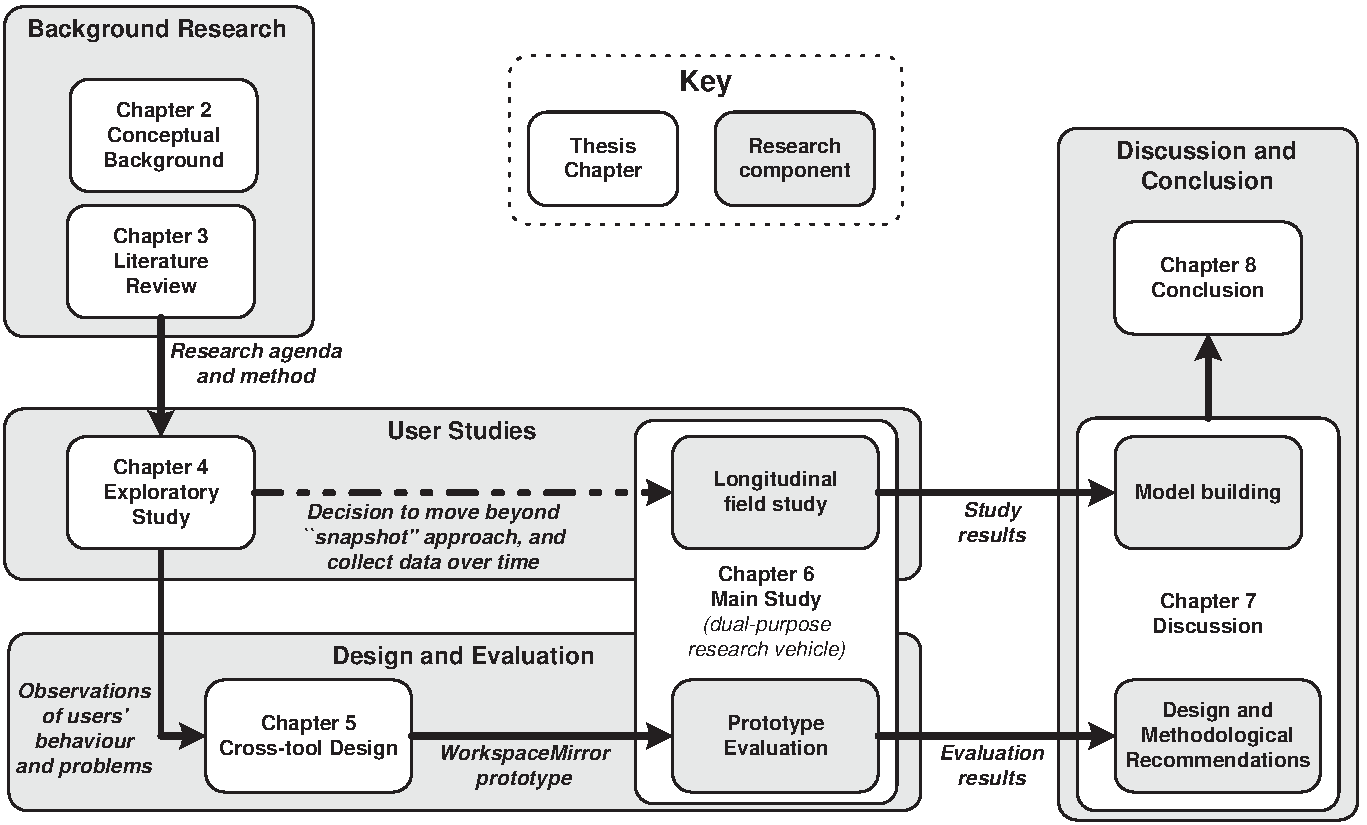
\includegraphics[width=1.0 \textwidth]{pictures/intro/Ch1-ThesisMap.pdf}
	\end{center}
	\caption{Overview of Thesis Structure} % \textit{Add contributions?}}
	\label{fig:intro:thesis_map}
\end{figure}

%%%%%%%%%%%%%%%
% Chapter 2: CF
%%%%%%%%%%%%%%%
% provides background for the thesis by reviewing related work within HCI and related disciplines. The chapter closes by discussing the initial aims which set the agenda for this research programme.
% details current support for PIM
% A conceptual framework relating to PIM. A descriptive vocabulary for discussing PIM as an activity, and the PIM-tools which enable it
% My Cross-tool Research Perspective/Analysis/Model of PIM. Provides theoretical framework for analysing user activity, user needs, discussing design, evaluation/study methodologies and results. Analysis of use of perspective.
% \item A high-level \textbf{conceptual framework} for PIM is proposed in \textbf{Chapter~\ref{chapter:bg}}. The framework defines terms used later in the thesis.  In particular a focus is taken on the integration of PIM-tools (\textit{substantive/minor}). 
% defines a number of concepts relevant to the thesis. 
% In this chapter, the author develops a \textit{conceptual framework} that 
\textbf{Chapter~\ref{chapter:bg}} provides an in-depth introduction to PIM.  Previous definitions of PIM are criticised, and a new view of PIM is developed in terms of four sub-activities performed with a collection of items: acquisition, organization, maintenance and retrieval.  Further conceptual background is provided relating to the current generation of commonly available PIM-tools. In particular, the concept of PIM-integration is defined and current integration mechanisms are surveyed.



%%%%%%%%%%%%%
% Chapter 3: REVIEW
%%%%%%%%%%%%%
% justification of techniques
% Critically assess
% \item A \textbf{critical review} of related research is presented in \textbf{Chapter~\ref{chapter:review}}. The review identifies a number of limitations of previous work, and motivates the research performed in the thesis (\textit{substantive/minor}).
\textbf{Chapter~\ref{chapter:review}} presents a \textit{critical analysis of previous research relevant to this thesis}.  Two main bodies of research are identified and surveyed: (1) empirical studies, and (2) prototype design.  Relevant theoretical work is also discussed. Limitations in prior research in the area of PIM-integration are used to motivate the thesis research agenda and methodology.  In particular, the limitations of previous technological research centred on radical invention are used to motivate the incremental design approach used in this thesis.

%%%%%%%%%%%%
% Chapter 4: EXP STUDY
%%%%%%%%%%%%
% \textit{Chapter 4 presents an exploratory study that compares how individuals manage their files, email and bookmarks. The potential for integrating these three tools is explored.}
% Add generation of scenarios?
% This chapter forms an empirical foundation for the rest of the thesis -- providing requirements and motivation for the design in \textbf{Chapter~\ref{chapter:design}}.  
\textbf{Chapter~\ref{chapter:exploratory_study}} reports an exploratory study aimed at comparing PIM behaviour across three collections of personal information -- document files, email and web bookmarks. The work can be contrasted with previous PIM studies which have focused on behaviour within one tool such as email. Key contributions include:
\begin{itemize}
%%%%%%%%%%%%%%%%%%%%%%%%
% EXP STUDY FINDINGS
%%%%%%%%%%%%%%%%%%%%%%%%
%  user requirements for improved integration between PIM tools
% Provide further understanding of PIM from a holistic "cross-tool" perspective. Use to differentiate.
% Probably want to break down in more detail!
% \item Further understanding of the nature of PIM in three specific tools (files, email and bookmarks), including new classifications of filing strategies in each tool, to reflect the observation of multiple strategies (\textit{substantive/minor}).
\item \textit{A comparison of PIM behaviour between files, email and bookmarks}  -- This analysis is centred on the four PIM sub-activities identified in \textbf{Chapter~\ref{chapter:bg}}.  % A particular focus is taken on the organizing sub-activity.

\item \textit{A new classification of organizing strategies in the file, email and bookmark contexts} -- Observations are made of \textit{multiple strategies} in each tool-specific context. Previous classifications of organizing strategies are criticized for not reflecting this  level of detail.  

% Third, a method for building a cross-tool profile of a user's management strategies.
% organizing strategies between tools for individual users.
\item \textit{A comparison of users' organizing strategies between files, email and bookmarks} -- Evidence is provided of variation in the extent of organizing performed by many participants across files, email and bookmarks.  A theoretical model is proposed to describe the multiple strategies observed both within and between collections.

% This major contribution encompasses three methodological contributions.
%%%%%%%%%%%%%%%%%%%%%
% ORG DIMENSION ANALYSIS
%%%%%%%%%%%%%%%%%%%%%
% First, a method for comparing folder structures in terms of their organizational dimensions on which folders are based.  
% analysing the organizational dimensions used to name folders in each tool context} --
\item \textit{A new technique for analysing the organizational dimensions used to name folders in each tool context} -- The most common types of folder are compared between the three tools.

%%%%%%%%%%%%%%%%%%%
% FOLDER OVERLAP ANALYSIS
%%%%%%%%%%%%%%%%%%%
% Second, a method for investigating the folder overlap between different PIM-tools for a particular user.  
\item \textit{A new technique for assessing the similarity of folder structures in two PIM-tools in terms of the number of folders they have in common} -- Significant folder overlap is highlighted for many participants, particularly between files and email.

%%%%%%%%%%%%%%%%%%%
% DESIGN RECOMMENDATIONS
%%%%%%%%%%%%%%%%%%%
\item \textit{A series of design implications for PIM-integration mechanisms} -- A number of PIM-related problems are identified which bridge multiple tool contexts, confirming the promise of improved integration between PIM-tools.  The above empirical findings suggest a number of potential routes for the design of such mechanisms.  In particular, the \textit{folder overlap} results provide the key empirical motivation for the design work in \textbf{Chapter~\ref{chapter:design}}.

\end{itemize}
% The study findings include the detailed analysis of similarities and differences between PIM practices across the three tools. 

%%%%%%%%%%%%%%%%%%%%%%%%%%%%%%%

%%%%%%%%%%%%%%%%%%%%%%%%%%%%%%%

%%%%%%%%%%%%%%%%%%%%%%%
% PART 2
% Chapter 5: DESIGN
%%%%%%%%%%%%%%%%%%%%%%%
% The second part of the thesis puts the developed cross-tool methodology into practice.
% \textit{Chapter 5 reports the design of WorkspaceMirror, motivated by the observation of folder overlap in Chapter 4.}
% The design is proposed as a research vehicle to: (1) explore the potential to improve integration between PIM tools, (2) develop appropriate methodology for evaluating PIM tools.  The chapter closes with an initial feasibility study to assess the potential of WorkspaceMirror.  Contributions from thesis are as follows:
% Cross-tool design of WorkspaceMirror and its implementation. Other designs? Why a useful contributions -- as design straw-man?
% \item The fourth main contribution, is the \textbf{design and implementation} of a prototype means of integration between PIM-tools, WorkspaceMirror, based on the folder-mirroring principle . The design is motivated by findings from the exploratory study (\textit{substantive/major}).  The notion of a cross-tool interactive artefact is also proposed (\textit{substantive/minor}).
\textbf{Chapter~\ref{chapter:design}} reports the cross-tool design and implementation work performed by the author.  In contrast to much previous design work in the area, the design approach is deliberately \textit{incremental} to facilitate user familiarity and systematic evaluation.  Contributions from the chapter are two-fold:
\begin{itemize}
% is informed by data from the exploratory study, WorkspaceMirror, a PIM-unification prototype designed and implemented by the candidate, is described.  
\item \textit{The design and implementation of WorkspaceMirror, a novel form of PIM-integration} -- The design is based on the principle of folder-mirroring, which allows the user to replicate the changes made in one folder structure to other PIM-tools.  A prototype is developed on the MS-Windows platform, offering folder-mirroring between the file, email and bookmark collections.  The design is motivated by the observations of \textit{folder overlap} in \textbf{Chapter~\ref{chapter:exploratory_study}}. 

\item \textit{Results from an initial evaluation of WorkspaceMirror} -- Positive feedback received from four of the five test users confirms the feasibility of the design.  The prototype is modified to accommodate participants' design suggestions.
\end{itemize}



%%%%%%%%%%%%%%%%%%%%%%%%
% Chapter 6: MAIN STUDY
%%%%%%%%%%%%%%%%%%%%%%%%
\textbf{Chapter~\ref{chapter:main-study}} reports a longitudinal field-study which acted as a dual-purpose research vehicle to: (1) evaluate the WorkspaceMirror prototype proposed in \textbf{Chapter~\ref{chapter:design}}, and (2) investigate PIM behaviour over time.  The investigation is differentiated from most previous studies in the area which have consisted of short-term ``snapshots'' of user behaviour.  A wide range of behaviour is reported through a series of case studies which highlight the idiosyncratic nature of PIM.  Two major sets of substantive contributions are offered: 
\begin{itemize}
%%%%%%%%%%%%%%%%%%%%%%%%%
% MAIN STUDY/EVALUATION
%%%%%%%%%%%%%%%%%%%%%%%%%
% Findings from combined Cross-tool Longitudinal Study/Formative Evaluation
%% A case-study evaluation (evaluation is hard to do
% Firstly, WorkspaceMirror is evaluated resulting in a number of proposed design improvements.
% aimed at investigating the impact of WorkspaceMirror on PIM practice. The evaluation involved eight users trialling WorkspaceMirror over a period of several months. The study also acted as a \textbf{longitudinal study} of PIM practice. In contrast most previous studies have consisted of ``snapshots'' of user behaviour.  
\item \textit{Results from the formative evaluation of WorkspaceMirror} -- The evaluation confirms the potential of mirroring top-level folders between PIM-tools, based on the positive feedback from many participants.  However, a trade-off is identified between the resulting consistency between folder structures, and users' needs for organizational flexibility in different tools.  A large number of design improvements are also suggested including the need for improved configurability.

%%%%%%%%%%%%%%%%%%%%%%%%%
% MAIN STUDY/STUDY
%%%%%%%%%%%%%%%%%%%%%%%%%
% \item Secondly, results from the longitudinal study of PIM over several months, including an analysis of changes in PIM strategy over time (\textit{substantive/major}). 
\item \textit{Insights into longitudinal PIM behaviour} -- Most study participants did not make major changes in organizing strategy.  Instead, \textit{incremental changes} were observed for two participants.  Balter's model of PIM strategies is criticised for not reflecting such subtle changes, and a new descriptive model is proposed.

The study findings also emphasise the background, supporting nature of PIM, and suggest that the participants devote little ongoing attention to PIM compared to their work tasks.  The study intervention causes increased reflection on PIM for many participants.  %  of findings are reported that suggest that participants rarely reflect on their PIM strategies. %, and instead are more focused on their work.

\end{itemize}
% \textit{Chapter 6 reports a field-study evaluation of WorkspaceMirror.}




%%%%%%%%%%%%%%
% Chapter 7: DISC
% WHERE IS THEPORY BUILDING?
%%%%%%%%%%%%%%
\textbf{Chapter~\ref{chapter:discussion}} discusses the substantive findings from the previous three chapters. The discussion offers four main contributions:
\begin{itemize}

% Extensions Barreau's PIM model~\citep{barreau:95} are proposed to encompass the supporting, ongoing, and cross-tool aspects of PIM, as identified in the empirical work in \textbf{Chapters~\ref{chapter:exploratory_study}}  and \textbf{~\ref{chapter:main-study}}. The chapter also considers implications for future work directed towards the design of more coherent, integrated PIM technologies.  The following contributions are offered:
% \item The main theoretical contribution is an extension of Barreau's PIM model~\citep{barreau:95} to encompass the ongoing, cross-tool supporting nature of PIM (\textit{substantive/major}). The model is based on empirical results from \textbf{Chapters~\ref{chapter:exploratory_study}} and\textbf{~\ref{chapter:main-study}}.
\item \textit{An extended conceptual framework of PIM} -- The view of PIM outlined in \textbf{Chapter~\ref{chapter:bg}} is extended to reflect the \textit{cross-tool}, \textit{supporting}, and \textit{ongoing} nature of PIM.  Each property is illustrated by reference to the empirical findings in earlier chapters.  The author offers the framework to outline potential routes for future theory development in the area.

%  The final substantive contribution is a set of recommendations for appropriate design routes for the design of mechanisms for improving integration between PIM-tools (\textit{substantive/major}).
\item \textit{A set of design implications for PIM-integration mechanisms} -- The evaluation results are discussed in the context of the extended framework.  Based on the experience of designing and evaluating WorkspaceMirror, the author argues that integration designs may offer strengths and weaknesses in different tool-specific and cross-tool contexts.  A number of design routes are highlighted for future integration work.

% Recommendations are made for appropriate methodology for evaluating PIM-tools based on experiences in evaluating WorkspaceMirror (\textit{methodological/minor}).
\item \textit{A set of methodological recommendations} -- The theoretical framework is used to structure a series of recommendations to guide the design and evaluation of PIM-integration mechanisms, derived from the experience of pursuing this research programme.  In particular, the dilemma of designing tools for supporting activities such as PIM is highlighted.

\item \textit{An exploration of potential evaluation metrics based on user experience} -- A number of participants in the main study reported in \textbf{Chapter~\ref{chapter:main-study}} were dissatisfied with their current organizing strategies and wanted to change them.  Such ``unsettledness'' is proposed as a indication of negative user experience in PIM.

\end{itemize}



%%%%%%%%%
% CONC
%%%%%%%%%
% before outlining potential future work. Chapter 8 presents overall conclusions, summarizes main contributions
% ties together
% bring together themes
% summarises
\textbf{Chapter~\ref{chapter:conclusion}} concludes the thesis by summarizing the main findings and contributions from the thesis.  Limitations of the research, and routes for further work are presented. % \footnote{\textit{This draft of Chapter 1 INTRODUCTION was printed \today}}.



%%%%%%%%%%%%%%%%%%%%%%%%%%%%%%%%%%%%
% Significance: major/minor (Weiss-Lijn)
% Audience: researchers/designers
% substantive and methodological
%%%%%%%%%%%%%%%%%%%%%%%%%%%%%%%%%%%%
% This thesis offers the following contributions. They are classified in terms of having a methodological or substantive nature, and their level of significance (major/minor):
% The section also considers their audience of interest (designers/researchers):%
% \begin{enumerate}

%%%%%%%%%%%%%%%%%%%%%%%%%%%%%%%%
% OTHER CONTRIBUTIONS TO CONSIDER
%%%%%%%%%%%%%%%%%%%%%%%%%%%%%%%%
% THINK: consideration of non-professional, social users?}
%%%%%%%%%%%%%%%%%%%%%%%%%%%%%%%%%%%%%%
% Methodological Contributions}
%%%%%%%%%%%%%%%%%%%%%%%%%%%%%%%%%%%%%% \textbf{M2: Methodological}. Operationalization as Cross-tool Methodology. Appraisal/analysis of use/validity of cross-tool method.

%%%%%%%%%%%%%%%%%%%%%%%%
% FIN: CONTRIBUTIONS
%%%%%%%%%%%%%%%%%%%%%%%%


%%%%%%%%%%%%%%%%%%%%%%%%%%%%%%
% Other possible challenges
%%%%%%%%%%%%%%%%%%%%%%%%%%%%%%
% Lots of commercial effort in terms of interface development.

%%%%%%%%%%%%%%%%%%%%%%%%%%%%%%%%%%%%%%%%%%%%%%%%%%%
\subsection{Publications relating to this Thesis}
%%%%%%%%%%%%%%%%%%%%%%%%%%%%%%%%%%%%%%%%%%%%%%%%%%%

The author has published a number of papers relating to this thesis work.  \citet{rpb:01b, rpb:01a} reports provisional results from the exploratory cross-tool study reported in \textbf{Chapter~\ref{chapter:exploratory_study}}. %, including the analysis of \textit{folder overlap}.

A subsequent series of papers report the design of WorkspaceMirror, along with the empirical results which motivated it~\citep{rpb:02b,rpb:02a,rpb:02c}. \citet{rpb:03a} adds preliminary results from the initial evaluation of WorkspaceMirror.

\citet{rpb:04a} presents a cross-section through the entire thesis, reporting aspects of the exploratory study, the design of WorkspaceMirror, and the longitudinal study. % presented in \textbf{Chapter~\ref{chapter:main-study}}.

Finally, \citet{rpb:04b}, outlines a Special Interest Group on PIM at the ACM CHI 2004 conference. The event has contributed to the establishment of a new PIM research community.  %  to 




% %%%%%%%%%%%%%%%%%%%%%%%%%%%%%

% chapter 2 - Background

% %%%%%%%%%%%%%%%%%%%%%%%%%%%%%

% \chapter{Background\label{chapter:review}}

\chapter{Conceptual Background}

\label{chapter:bg}

% \textit{CHAPTER 2 LEFT INTENTIONALLY BLANK AS A PLACEHOLDER}


%%%%%%%%%%%%%%%%%%%%%%%%%%%%%%%%%%%%%%%%%%%%%%%%%%%%%%%%%%%%%%%%%%%%%
% Richard Boardman rick@ic.ac.uk
% PhD Thesis - Department of Electrical and Electronic Engineering
% Imperial College London SW7 2BT UK
% %%%%%%%%%%%%%%%%%%%%%%%%%%%%%%%%%%%%%%%%%%%%%%%%%%%%%%%%%%%%%%%%%%%
% Improving Tool Support for Personal Information Management
% Chapter 2: Background
% Version 96, 22nd May 2004
%%%%%%%%%%%%%%%%%%%%%%%%%%%%%%%%%%%%%%%%%%%%%%%%%%%%%%%%%%%%%%%%%%%%%

%%%%%%%%%%%%%%%%%%%%%%%%%%%%%%%%
\section{Introduction}
\label{bg:intro}
%%%%%%%%%%%%%%%%%%%%%%%%%%%%%%%%

%%%%%%%%%%%%%%%%%%%%%%%%%%%%%%%%
% \section{Overview of the Chapter}
%%%%%%%%%%%%%%%%%%%%%%%%%%%%%%%
This chapter provides a conceptual grounding to the research in this thesis, and defines the key terminology used in subsequent chapters. %\footnote{This draft of ``Chapter 2 Background'' was printed \today}.

\textbf{Section~\ref{bg:pim}} provides an overview of Personal Information Management (PIM) as a fundamental aspect of computer-based activity.  \textbf{Section~\ref{bg:pim-defns}} discusses the limitations of previous definitions of PIM. Then, \textbf{Section~\ref{bg:pim-activity-cf}} outlines the view of PIM taken up in this thesis, building on the conceptual framework offered by~\citet{barreau:95}.  Lastly, \textbf{Section~\ref{bg:pim-relatedterms}} contrasts PIM with related terms such as information retrieval and information management.
% The conceptual framework builds on previous theory in the area~\cite{barreau:95}.

% provides background on software tools that support the activity of personal information management.
The second part of the chapter, \textbf{Section~\ref{bg:pim-tools}}, is concerned with the software tools that support PIM, termed \textit{PIM-tools} in this thesis. 
Firstly, \textbf{Section~\ref{bg:pimtool-defn}} defines the term PIM-tool, and describes an abstract model of a canonical PIM-tool. 
The next three sections consider the past, present, and future of PIM-tool technology.
\textbf{Section~\ref{bg:pim-history}} discusses the history of PIM-tools,  \textbf{Section~\ref{bg:current-survey}} surveys the current generation of PIM-tools, and \textbf{Section~\ref{bg:trends}} highlights a number of ongoing trends in PIM-tool design. 
Finally, \textbf{Section~\ref{bg:integration}} discusses the concept of \textit{integration between PIM-tools}, a central theme to this thesis.
% A second conceptual framework is developed in \textbf{Section~\ref{bg:pimtool-cf}} outlining a  personal information management tool
% from the first provisions of mainframe operating systems for personal storage space for users.  
% Finally \textbf{Section~\ref{bg:conclusion}} presents the chapter's conclusions and summarizes contributions towards the overall thesis.


%%%%%%%%%%%%%%%%%%%%%%%%%%%
%%%%%%%%%%%%%%%%%%%%%%%%%%%
%%%%%%%%%%%%%%%%%%%%%%%%%%%
%%%%%%%%%%%%%%%%%%%%%%%%%%%

\newpage
%%%%%%%%%%%%%%%%%%%%%%%%%%%%%%%%%%%%%%%%%%%%
\section{Personal Information Management}
\label{bg:pim}
%%%%%%%%%%%%%%%%%%%%%%%%%%%%%%%%%%%%%%%%%%%%
%% 	\item \textbf{Pervasive human activity} -- both digital and physical. 
%% define object
%% Somewhat of an overlap with the intro chapters
%% Expand on ongoing nature - use throughout the day. Small incremental changes
%% Need to talk about USER as well as TOOL and TASK

%%%%%%%%%%%%
% 2 domains
%%%%%%%%%%%%
A fundamental characteristic of human nature is to collect. In both the physical and digital domains, our personal environment (e.g. desk, wallet, computer desktop) becomes populated with the objects we accumulate as our lives unfold.

% VALUED MATERIAL
Some of these objects are acquired intentionally. We choose to keep a subset of the objects that we encounter -- those of some perceived value to us. The notion of value varies widely between the objects we keep. A brief perusal of the author's desk, the physical environment in which this thesis is being written, reveals a range of objects valued for varying reasons:  postcards kept for sentimental reasons, documents containing information required in the writing process, a cycle helmet. All these objects are valued in relation to some aspect of the author's ongoing roles and activities.
% STUFF THAT IS NOT VALUED
As well as valued material, our environments fill up with other less important objects.  This ``excess baggage'' may include objects that were once valued, but for reasons that have been long-forgotten. Other objects we do not even choose to acquire -- they just seem to appear as an implicit by-product of our lives -- for example receipts and junk mail.  Although we may wish to discard of such objects, the time and effort involved in dealing with them can be so high that we put off doing so, and they accumulate in our personal environment. % until we take the time to deal with them.
%% It may annoy us for reasons of untidiness

% Each of us makes a personal choice about how much time to devote to the management of our individual environment.
Our lives are filled with personal decisions relating to managing our possessions: what to acquire, whether and how to organize it, what to throw away, and how to go about finding things when we require them. Unless influenced by an external constraint such as a corporate clean-desk policy, this managing activity is inherently idiosyncratic.  % Two people doing the same job in the same organization are free to employ totally dissimilar management strategies.  % For example, in his study of office organization,~\citet{tm:83} noted two extremes, the \textit{messy} and the \textit{tidy}.
%% Thus it is a discretionary activity (CHECK Landauer).

Over the ages, many artefacts have been created to help people to manage the objects they collect in the physical domain.  Today, many of these are taken for granted.  For example, \citet{norman:93} discusses the invention in the late nineteenth century of the seemingly humble filing cabinet.   At the time, this device revolutionized the management of document archives.  Norman discusses the \textit{cognitive scaffolding} offered by such artefacts: they allow people to offload the overhead of organizing -- and remembering how things are organized when they need to find them -- onto the environment.
%% The humble filing cabinet is not often considered a revolutionary device in the way that Norman describes it.
%% \textit{Previous to this ...}

%% \textbf{Establish focus on digital-PIM via background in PIM-general}:
The dramatic boom in personal computing technology over the past two decades means that people now manage personal collections of \textit{digital} objects in addition to the physical objects they manage in the real-world.  Today millions of personal computer users collect and manage a wide range of digital objects such as email messages, music files, contacts, and web bookmarks.
% This digital collecting activity occurs in both home and work contexts.
%%  The term \textit{information} is used in this thesis as a general term for the various forms of digital object that people collect.
%%
%% Use of digital tools to make it easier for us
%%
%% add survey quote x% of people/households have personal computers
% Over the first quarter of 2003 an estimated 11.7 million households in the UK could access the Internet from home representing 47 per cent of all households. This is nearly twice the number three years earlier and is a continued increase from the 43 per cent reported in the first quarter of 2002.
% Retrieved from http://www.statistics.gov.uk/STATBASE/ssdataset.asp?vlnk=6935
% Expenditure and Food Survey, UK July 2003, Office National Statistics (retrieved 3 November 2003)
The term \textit{Personal Information Management}, often abbreviated to PIM, is used as an umbrella term to describe the everyday process performed by individuals as they collect, store, organize and access their collections of digital objects.  As in the physical world, a range of technologies have been developed to help people in this process, such as the folder hierarchy and search mechanisms.  This thesis aims to contribute to the HCI knowledge base to better guide the designers of such technology.
% The next section moves on to survey previous definitions of PIM from the literature.
% \textbf{Section~\ref{bg:pim-defns}} moves on to survey previous definitions of PIM. 
%% Personal Information Management (PIM) has been proposed as an umbrella term to describe the  of digital objects by an individual in their personal computing environment~\cite{lansdale:88, }. 
% In the physical world, the accumulation of information resources, typically in the form of various types of paper-based documents, is a familiar feature of our personal environments, both at work and at home.  Examples: wallet (Levy p120,~\cite{pearce:99,norman:93}). In fact physical-PIM has become driving force for much work in HCI through studies such as~\cite{tm:83}.




%%%%%%%%%%%%%%%%%%%%%%%%%%%
%%%%%%%%%%%%%%%%%%%%%%%%%%%
%%%%%%%%%%%%%%%%%%%%%%%%%%%
%%%%%%%%%%%%%%%%%%%%%%%%%%%

%%%%%%%%%%%%%%%%%%%%%%%%%%%%%%%%%%%%%%%%%%%%%%%%%%%%%%%%%%%%
\subsection{Previous Definitions}
\label{bg:pim-defns}
%%%%%%%%%%%%%%%%%%%%%%%%%%%%%%%%%%%%%%%%%%%%%%%%%%%%%%%%%%%%
%% Word: imprecise definition
%% The term personal information management has not been tightly defined in the literature.
%% Think about Barreau's framework as a basic task decomposition, although one that is ONGOING
% In this section previous definitions of personal information management are surveyed. These definitions focus on personal information management as an everyday activity carried out by computer users.
%% \textit{Is copying and pasting a paragraph of text between documents personal information management?}
%% ADD: why is a definition important?
%%%%%%%%%%%%%%%%%%%%%%
% SIMPLE definition
%%%%%%%%%%%%%%%%%%%%%%
% PIM is information management as performed by an individual user for their own needs. 
% PIM can be defined very simply as \textit{information management performed by an individual for their own needs}.  However, such a high-level definition does not define what the information is being managed, and what constitutes ``management''.

%%%%%%%%%%%%%%%%%%%%%%%%%%%%%%%%%%%%%%%
% Lack of consensus on a definition
%%%%%%%%%%%%%%%%%%%%%%%%%%%%%%%%%%%%%%%
% Terms used in different ways, e.g. ``archiving''
\citet{Whittaker-rta:00} observe the lack of systematic research within Human-Computer Interaction (HCI) on many everyday computing activities including PIM.  One problem they identify is the lack of consensus regarding the definition of key terms.  This means that researchers doing new work in the area add new definitions to the wide range of candidates already available.  This section surveys some previous definitions of PIM and argues the need for a more systematic definition.

%%%%%%%%%%%%%%%%%%%%%%%%%%%%
% PIM = store to retrieve?
%%%%%%%%%%%%%%%%%%%%%%%%%%%%
Many definitions of PIM draw from a traditional information management perspective -- that information is stored so that it can be retrieved at a later date.  For example,~\citet{Bellotti:02a} describe PIM as: \textit{``the ordering of information through categorization, placement, or embellishment in a manner that makes it easier to retrieve when it is needed''}.  Such definitions are founded on the assumption that information is stored to facilitate later retrieval.
%%  It may also involve a great deal of information related to coordination and collaboration (collaborative information management). It may involve resources such as piles, collections, file hierarchies, notes, to-do lists, calendars, contact managers and so on."'}.
% Thus there is more to personal information management than is reflected in the above definitions.
%% recall/recognition and classification


%%%%%%%%%%%%%%%%%%%%%%%%%%%%
% What about reminding?
%%%%%%%%%%%%%%%%%%%%%%%%%%%%
% %% We need to look beyond the traditional information management perspective that focuses on storing items for future retrieval.
% (i.e. to contextualize their work activity).
Similarly, \citet{ml:88} defines PIM as \textit{``the methods and procedures by which we handle, categorize, and retrieve information on a day-to-day basis''}.  However, Lansdale notes that enabling retrieval is only one reason for managing information, referring to the work of \citet{tm:83} who observed the \textit{reminding} affordance of paper documents.  Malone describes how people do not only manage documents to find them again, they also do so to remind themselves of tasks to perform.  Although Lansdale acknowledges the various ways in which information can be used, his definition can be criticized for not defining what is meant by ``handling''.

%%%%%%%%%%%%%
% BARREAU
%%%%%%%%%%%%
% She conceptualizes a PIM system as \textit{``an information system developed by, or created for, an individual in a work environment''}.  
\citet{barreau:95} conceptualizes  a PIM system as \textit{``an information system developed by, or created for, an individual in a work environment''}.  She considers how a PIM system enables the construction of a collection of items, which constitute a personal information space. Barreau describes five functions provided by a PIM system:
% Barreau's definition highlights the fact that personal information management is a high-level activity, one that consists of multiple sub-activities.

\begin{enumerate}

%%%%%%%%%%%%%%%%%
% ACQUISITION
%%%%%%%%%%%%%%%%
%% Barreau: the methods and rules by which information is added to the system.
% (e.g. the creation of information by the user, or the downloading of information from the internet).
\item The \textit{acquisition} of items into the PIM system, including the definition, grouping, and naming of new information (e.g. the saving of newly created or downloaded information).

%%%%%%%%%
% ORG
%%%%%%%%%
\item The \textit{organization} of items within the system (e.g. filing items into folders). 
%% Barreau notes the different classifying rules used based up on the level of granularity of the workload being supported

%%%%%%%%%%%%%%
% MAINTENANCE
%%%%%%%%%%%%%%
% (e.g. deleting items, backing up items, archiving items, and updating items). 
% Barreau: dictated by circumstance
% Barreau: update, delete, archive, backup
\item The \textit{maintenance} of the system in terms of updating, archiving and deleting items\footnote{Another source of terminological confusion in the area is the lack of definition for terms such as \textit{archiving}. Some researchers use archiving to refer to the filing of an item within a folder, e.g.~\citep{Whittaker-email:96}.  In this thesis, Barreau's interpretation of archiving is employed: the removal of an item from a collection for storage elsewhere.}.

%%%%%%%%%%%%%%
% RETRIEVAL
%%%%%%%%%%%%%%
\item The \textit{retrieval} of items via search or browsing, as driven by the user's information needs.
% Common retrieval mechanisms include the browsing of items arranged in semantic categories (e.g. folders) or spatially on the desktop, sorting items in order of metadata, or content/keyword-based searching.

\item The \textit{presentation} of retrieved information in an appropriate output format. % (\textit{``the procedures for producing the various outputs desired''})

\end{enumerate}

%%%%%%%%%%%%%%%%%%%%%%%%%%%%%%%
% TOWARDS A NEW DEFINTION
%%%%%%%%%%%%%%%%%%%%%%%%%%%%%%%
%Another limitation of previous definitions is that they do not specify what constitutes information, and what is special about personal information.
%However these definitions do not define personal information or what constitutes management.  Barreau comes the closest but has several limitations as follows:
%\begin{enumerate}
%\item She limits to work
%\item She includes ``editing'' -- surely then this involves everything performed on a computer
%\end{enumerate}
%\textbf{Section~\ref{bg:pim-activity-cf}} builds on these previous definitions by building up a conceptual framework relating to personal information management.
Although Barreau's definition conveys the multi-faceted nature of ``handling'' items, it can be criticized on several counts.  Primarily, she includes the \textit{updating} of items in her definition of the maintenance aspect of PIM.  In contrast, the author takes the view that updating items (e.g. editing a file or a diagram) is not part of PIM.
% In particular, PIM is explicitly distinguished from the modification of information. 
Rather than proposing a brand new definition, the next section modifies Barreau's framework to deal with this and a number of other limitations.  This new definition represents the view of PIM taken up in this thesis. %, and is later used to define the term PIM-tool.

% Firstly, definitions of \textit{information} and \textit{personal information} are offered.  It is argued that ``personal information'' in particular is an ambiguous term that requires careful specification.





%%%%%%%%%%%%%%%%%%%%%%%%%%%%%%%%%%%%%%%%%%%%%%%%%%%%%%%%%%%%%%%%%%%%%%%%%%
\subsection{Defining Personal Information Management Step by Step}
\label{bg:pim-activity-cf}
%%%%%%%%%%%%%%%%%%%%%%%%%%%%%%%%%%%%%%%%%%%%%%%%%%%%%%%%%%%%%%%%%%%%%%%%%%
%%
%%The following criticisms can be levelled at definitions to date:
%%\begin{enumerate}
%%	\item All three of these definitions is the assumption that the fundamental reason for managing information is to facilitate its retrieval at a later date.
%% \end{enumerate}

This section builds up a step-by-step definition of PIM in three stages:
%% The definition consists of the following three stages:
\begin{enumerate}

\item Firstly, a definition of \textit{information} is presented.
\item This is specialized to form a definition of \textit{personal information}.
\item The final step is to define the term \textit{PIM}.  This definition in turn used to define the functionality provided by a PIM-tool in \textbf{Section~\ref{bg:pim-tools}}.
\end{enumerate}

% The definition of personal information management is used in turn to define what it means for a software tool to support \textit{personal information management}, and to scope out the work carried out in the thesis.


%%%%%%%%%%%%%%%%%%%%%%%%%%%%%%%%%%%%%%%%%%%%%%%
\subsubsection{Defining ``Information''}
%%%%%%%%%%%%%%%%%%%%%%%%%%%%%%%%%%%%%%%%%%%%%%%
%% This is a very general definition and includes 
%% Need to cite definition of ``information''
%% bits/also known as content?
%% http://pespmc1.vub.ac.be/ASC/INFORMATION.html
%% that which reduces uncertainty. (Claude Shannon);
%% 2) that which changes us. (Gregory Bateson), Information is the meaning
% of the representation of a fact (or of a message) for the receiver.
%% Document -- Buckland
%% Bits -- Raskin
%% Angela -- data/information
%% Jens -- why not box in Excel?
%% Losee - Information may be defined as the characteristics of the output of a process, these being informative about the process and the input.  - http://www.ils.unc.edu/~losee/b5/book5.html
%% NB: this is personal information!! Are we jumping ahead?
%%%%%%%%%%%%%%%%%%%%%%%%%%%%%%%%%%%%%%%%%%%%%%%%%%
% http://www.aslib.co.uk/info/glossary.html
% Information: an assembly of data in a comprehensive form capable of communication and use 
% Knowledge: information evaluated and organised in the human mind so that it can be used purposefully
%%%%%%%%%%%%%%%%%%%%%%%%%%%%%%%%%%%%%%%%%%%%%%%%%%

% \textit{Information} is defined as any set of bits with carries meaning for an individual, such as text or a graphic image.
\textit{Information} has been defined as \textit{``an assembly of data in a comprehensive form capable of communication and use''}~\citep{IEILS:03}.  Here, information is defined more loosely as any assembly of data which carries some meaning for one or more people. % Indeed, it may not necessarily be useful or communicable. 
% What is crucial, is that it means something to one or more people.
This thesis focuses on information in the digital domain: arrangements of bits which carry meaning for one or more people, for example a paragraph of text or an image.  Henceforth, the term information is used to designate information in a digital context.  The next stage is to distinguish \textit{personal information} from information in general.




%%%%%%%%%%%%%%%%%%%%%%%%%%%%%%%%%%%%%%%%%%%%%%%
\subsubsection{Defining ``Personal Information''}
%%%%%%%%%%%%%%%%%%%%%%%%%%%%%%%%%%%%%%%%%%%%%%%
%%%%%%%%%%%%%%%%%%%%%%%%%%%%%%%%%%%%%%%%%%%%%%%
% \subsubsection{Alternatives interpretations of ``Personal Information''}
%%%%%%%%%%%%%%%%%%%%%%%%%%%%%%%%%%%%%%%%%%%%%%%
%%%%%%%%%%%%%%%%%%%%%%%%%%%%%%%%%%%%%%%%%%%%%%%%%%%%%%%
%% Add contrast with private information (see above)
%%%%%%%%%%%%%%%%%%%%%%%%%%%%%%%%%%%%%%%%%%%%%%%%%%%%%%%
%% Consider created/downloaded by user
%%%%%%%%%%%%%%%%%%%%%%%%%%%%%%%%%%%%%%%%%%%%%%%%%%%%%%%%%%%%%%%%%%
%% Need to define static/dynamic/executable/binary information
%%%%%%%%%%%%%%%%%%%%%%%%%%%%%%%%%%%%%%%%%%%%%%%%%%%%%%%%%%%%%%%%%%
\textit{Personal information} is an ambiguous term with a number of possible interpretations.
\begin{enumerate}

\item One interpretation is \textit{information about an individual} (i.e. where that individual is the subject matter of the information).  One common context for this usage is to describe the information stored by an institution about an individual  (e.g. date of birth, credit card number).  In this case, the information is not directly managed by the individual concerned.

\item A second interpretation is \textit{the information managed and stored within personal organizer software} ~\citep{web-rosenberg:99}.  In this sense digital personal information includes appointments, contacts, and to-do items -- but not information stored outside that specific tool, such as files stored in the file system. 
%%
%% Check Chandler

\end{enumerate}

%%%%%%%%%%%%%%
% DEFINITION
%%%%%%%%%%%%%%
% Notice that the definition of personal information used in the thesis is independent of technological format subsumes personal information stored in a personal organizer.	
% differentiates between personal information and private information. Personal information is that which is \textit{owned} by an individual, such as their files, diaries and books.  Private information is considered confidential by an individual, but is not necessarily owned by them.
% Note that Lansdale's definition does not specify what the subject matter of the information is -- what is crucial is that it is owned and actively managed by the individual.
% The individual is the subject of the information, but does not own the information: instead it is controlled and \textit{managed} by the . A common example is personal information recorded during the process of making a financial transaction on-line. Releasing such details to outside interests carries significant privacy implications and is the focus on significant development focus~\cite{p3p:03}.
%%%%%%%%%%%%%%%%%%%%%%%%%%%%%%%%%%%%%%%%%%%%%%%%%%%%%%%%%%%%
% NB: may not own in the legal sense
In the context of this thesis, personal information is defined as \textit{information owned by an individual, and under their direct control}.  In other words, the owning individual is able to alter or delete the information without going through an intermediary.  Note that this definition is independent of (1) the subject matter of the information, (2) the software application in which it is managed, and (3) the digital device on which it is stored.
%%%%%%%%%%%%%%%%%%%%%%
% UNITS OF ANALYSIS
%%%%%%%%%%%%%%%%%%%%%%
The units of analysis in this thesis are those of \textit{items} and \textit{collections} of personal information:
\begin{itemize}
%%%%%%%%%%%
% ITEM
%%%%%%%%%%%
% An \textit{item of information} is a self-contained unit of information (i.e. one that can exist in an independent form on a computer).
% In a personal computer, items of information are stored in a particular technological format such as file, email, bookmark, contact, calendar appointment and to-do item.  
% The term item is used to describe self-contained units of digital personal information such as 
\item An \textit{item} is a self-contained unit of information. In the digital domain, items of personal information exist in a range of \textit{technological formats} such as files, email, bookmarks, contacts, to-do item, and so on.  Note that in this thesis, a sentence or paragraph is not considered to be a unit of personal information, but rather a sub-unit.  Items may possess \textit{metadata attributes}, further information describing the content of the item.  Attributes may be system-defined (e.g. file size) or user-defined (e.g. title).  % Items may be classified within a semantic category (e.g. filed within the ``Chicago'' folder) or within a spatial category (e.g. placed in the top-left corner of the desktop).
%% Items contain \textit{information content} (the meaningful bits). 

%%%%%%%%%%%%%%%%%%%%%%%%%%%%%%%%%%%%
% A collection of information
%%%%%%%%%%%%%%%%%%%%%%%%%%%%%%%%%%%%
% A \textit{collection} of items of information is a stand-alone/self-contained set of items. 
\item A \textit{collection} of personal information is a self-contained set of items. Typically the members of a collection share a particular technological format and are accessed through a particular application\footnote{The main exception is the file system which can contain items (files) in a range of technological formats, e.g. spreadsheets, images and text documents.}.  Each collection can be considered as a \textit{personal information space} that is constructed by the user~\citep{da:98}. Example collections of personal information include electronic messages, managed with an email tool, and the set of contacts within an address book.

\end{itemize}
% In the context of a typical desktop computer, personal information includes all information stored in all applications, including personal organizers, files in the file system, contacts, calendar entries, email messages and so on.

% LINK FORWARD
% Note that digital personal information can exist on a range of devices -- for example computers, mobile phones and PDA devices. See next section.
% Based on this understanding of personal information, \textit{PIM} can now be defined.



%%%%%%%%%%%%%%%%%%%%%%%%%%%%%%%%%%%%%%%%%%%%%%%%%%%%%%%%%
\subsubsection{Defining ``Personal Information Management''}
%%%%%%%%%%%%%%%%%%%%%%%%%%%%%%%%%%%%%%%%%%%%%%%%%%%%%%%%%%
% \textbf{Classic HCI analysis}: the user, the tool, the task, context
%	\item Who is the user? -- everyone!
%	\item What is the tool? -- PIM tools
%	\item What is the activity? -- a long story!
%	\item And what about context of this activity?
% THINK: need to define each sub-activity in turn?
% Acquisition -a dding item to a collection and assigning metadata (explicit plus implicit)
%%%%%%%%%%%%%%%%%%%%%%%%%%
% DICTIONARY DEFINITION
%%%%%%%%%%%%%%%%%%%%%%%%%%
The Oxford English Dictionary defines ``management'' as \textit{``the process of dealing with or controlling things (noun), to be in charge of an undertaking, to administer, to regulate (verb)''}. 
%% amusingly also means to succeed (just) in achieving something difficult
%%%%%%%%%%%%%%%%%%%%%%
% PIM Definition
%%%%%%%%%%%%%%%%%%%%%%
%is here defined as the activity performed by an individual in
%the process an individual carried out in dealing with and controlling their collections of personal information.
Therefore, based on the above definition of personal information, PIM can be defined as \textit{the management of personal information as performed by the owning individual}.
% Furthermore that management activity is carried out for the individual's own needs.
%% an activity, carried out by an individual, of \textit{managing}, looking after, handling, their collections of personal information, their files, email and contacts. Thus the example is the management of an information by an individual for their own use.
%% The key is who is doing the management of the information by an individual for their own use. 
%% \textit{Construction of an information space. Customization of general-purpose workspace. Beyond storage and retrieval}
The conceptual framework offered by~\citet{barreau:95} is adopted in this thesis to denote the sub-activities that constitute ``management''.  However, a number of changes are made to Barreau's conceptualization as follows:
%		\item acquisition -- Archive as safekeeping (Levy).
%		\item storage/organization -- structure to handle complexity. Levy: anxiety of order, tidying
%		\item maintenance
%		\item retrieval.
% In this thesis, the following changes are applied to the framework:
\begin{enumerate}

%%%%%%%%%%%%%
% UPDATING
%%%%%%%%%%%%%
\item As noted above, Barreau included the \textit{updating} of information in her definition of the maintenance sub-activity.  Here the modification of items (e.g. editing of files) is considered outside the scope of PIM. Once an item of information is retrieved from a collection, it may be edited and re-saved (effectively re-acquired).  However what happens between the retrieval and re-saving is not considered part of PIM.
	
%%%%%%%%%%%%%%%%%%%%
% WORK OR LEISURE
%%%%%%%%%%%%%%%%%%%%
\item Barreau defines PIM as being carried out in a work context. Here it is defined as the managing of personal information in any context -- work or leisure.

%%%%%%%%%%%%%%%%%%%%%%%%%%%%%
%% FOUR PIM SUB-ACTIVITIES
%%%%%%%%%%%%%%%%%%%%%%%%%%%%%
%% Acquisition can be implicit or explicit. Two fundamental types: downloading, creation. Resaving
%%
%% Organization can also be implicit or explicit.
%% 
%% Finally retrieval can also be implicit or explicit -- search and browse.
%% 
%% \textbf{Different strategies for each sub-activity}  along with different motivations?
%% \textbf{Very complex/multifaceted activity} -- see section on nature of PIM below. e.g. ongoing, an activity in the large
%% 	\item Task granularity -- cue supporting/production discussion. NB even these sub-processes are complex!
\item Barreau defined PIM in terms of the functions provided by a PIM-system: \textit{acquisition}, \textit{organization}, \textit{maintenance}, \textit{retrieval} and \textit{output}.  In this thesis, PIM is conceptualized as a user activity.  
% \item Acquisition, organization, maintenance and retrieval of information can be \textit{explicit} (performed intentionally by the user) 
% In other words the other ``contextualizing'' functions such as reminding identified by~\cite{tm:83} are encompassed in the definition.
The first four of Barreau's functions equate to PIM sub-activities performed by a user: the \textit{acquisition} of items to form a collection of personal information, the \textit{organization} of items, the \textit{maintenance} of the collection, and the subsequent \textit{retrieval} of items. Barreau also highlights \textit{output} as a key PIM-system function.  Since this is performed automatically by the computer in current PIM tools, it is not included as a sub-activity.  Furthermore, reminding is not considered to be a PIM sub-activity.  Instead, the view is taken that items may be acquired and arranged (as part of PIM) to enable reminding.  \textbf{Figure~\ref{fig:chapter1_pim_model}} illustrates the view of PIM taken in this thesis.  

%Information is not only acquired and stored with the intent of retrieving it at a later date. As noted by Lansdale and Malone, an item information within a collection may simply act as a reminder. Indeed, information may not be retrieved at all.

\end{enumerate}



% %%%%%%%%%%%%%%%%%%%%%%%%%%%%%
% FIGURE - CONCEPTUALIZATION OF PIM
% %%%%%%%%%%%%%%%%%%%%%%%%%%%%%
\begin{figure}[hbtp]
	\begin{center}
		\leavevmode
		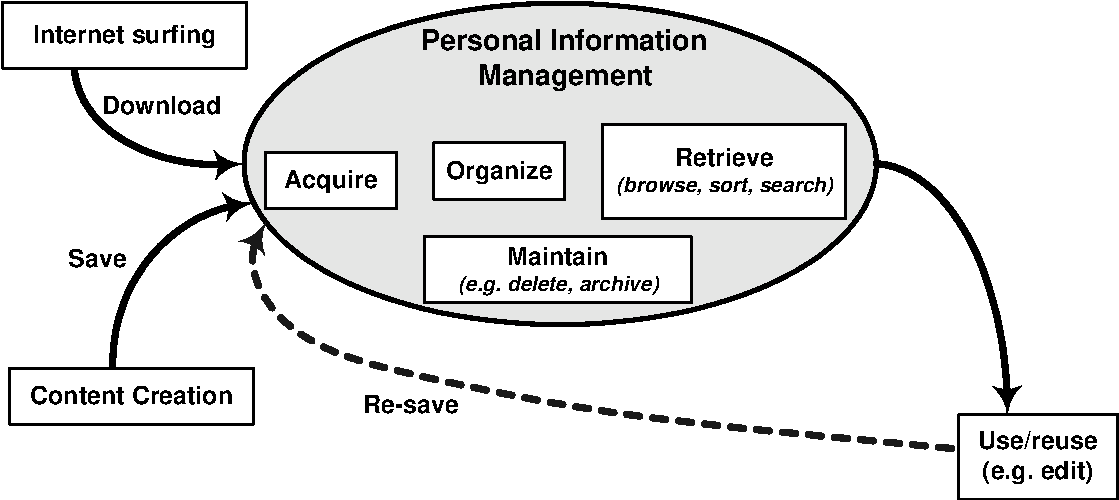
\includegraphics[height=4cm]{pictures/bg/BG-PimModel.pdf}
		\caption{Four PIM sub-activities: acquisition, organization, maintenance and retrieval}
		\label{fig:chapter1_pim_model}
	\end{center}
\end{figure}


%% Towards a distributed view
%% Cross-tool
%% Set of parallel/inter-related PIM systems
Barreau treats the computer as one monolithic PIM system, centred on the file system.  This thesis builds up the case that the computer is best conceptualized as a set of PIM systems, each denoted by the software application that allows a user to manage a collection of personal information in a particular technological format. Examples include the email collection, the bookmark collection, and the file collection.  For now this framework is offered as a description of the activities performed by an individual in each collection of personal information.
% This theme -- that the computer is best conceptualized as a set of parallel PIM systems -- is developed over the course of the thesis.




%%%%%%%%%%%%%%%%%%%%%%%%%%%%%%%%%%%%%%%%%%%%
\subsection{Comparison between PIM and Related Terms}
\label{bg:pim-relatedterms}
%%%%%%%%%%%%%%%%%%%%%%%%%%%%%%%%%%%%%%%%%%%%%%
 % Firstly, the term PIM is compared with related terms.
%c This section differentiates PIM from similar terms such as \textit{information management}, \textit{knowledge management}, and \textit{information retrieval}.

%% Relate to other "`applied"' areas \textit{(NB: generally these have been much more researched -- indeed IR has its own conferences)}:


%%%%%%%%%%%%%%%%%%%%%%%%%%%%%%%%%%%%%%%%%%%%%%%%%%%%%%%%%%%%%%%%%%%%%%%%
\subsubsection{Information Management}
%%%%%%%%%%%%%%%%%%%%%%%%%%%%%%%%%%%%%%%%%%%%%%%%%%%%%%%%%%%%%%%%%%%%%%%%
% http://www.aslib.co.uk/info/glossary.html
% Information: an assembly of data in a comprehensive form capable of communication and use 
% 
% Knowledge: information evaluated and organised in the human mind so that it can be used purposefully
% Information Management (IM): an imprecise term covering the various stages of information processing from production to storage and retrieval to dissemination towards the better working of an organisation; information can be from internal and external sources and in any format
% Knowledge Management (KM): again an imprecise term very similar to information management the main difference is the sharing (mapping) of information and experience of many individuals towards the betterment of an organisation, rather than information remaining with different individuals working separately towards the same goal
% The key difference between PIM and IM/KM is the entity which is carrying out the managing activity. 
\textit{Information Management} (IM) has been described as \textit{``the application of management principles to the acquisition, organization, control, dissemination and use of information relevant to the effective operation of organizations of all kinds''}~\citep{wilson:02a}.  In other words, the term IM typically relates to an organizational context\footnote{The term \textit{knowledge management} (KM) is sometimes used in a similar sense, somewhat controversially, to refer to IM as performed by a large institution such as a company~\citep{wilson:02b}.}. In contrast, with PIM, the scope of interest is limited to that of an individual user. % Indeed the PIM activities of all an organizations members can be seen to contribute to the overral 
%%  WILSON: Information here refers to all types of information of value, whether having their origin inside or outside the organization, including data resources, such as production data; records and files related, for example, to the personnel function; market research data; and competitive intelligence from a wide range of sources. Information management deals with the value, quality, ownership, use and security of information in the context of organizational performance}

%%%%%%%%%%%%%%%%%%%%%%%%%%%%%%%%%%%%%%%%%%%%%%%%%%%%%%%%%%%%%%%%%%%%%%%%
\subsubsection{General Information Management}
%%%%%%%%%%%%%%%%%%%%%%%%%%%%%%%%%%%%%%%%%%%%%%%%%%%%%%%%%%%%%%%%%%%%%%%%
\citet{Bergman:03} compare PIM with what they term \textit{General Information Management} in which a professional -- such as a librarian - manages information for other people.  PIM is differentiated by its focus on an individual managing information \textit{for his or her own use}.  Managing information for other users is outside the research scope of this thesis.
% An analogy in the physical world, would be that of a personal book collection compared with a library. 
%% information storage and retrieval
%% digital libraries (GIS)

%%%%%%%%%%%%%%%%%%%%%%%%%%%%%%%%%%%%%%%%%%%%%%%%%%%%%%
\subsubsection{Collaborative Information Management}
%%%%%%%%%%%%%%%%%%%%%%%%%%%%%%%%%%%%%%%%%%%%%%%%%%%%%%
%% \textit{Although may be side-effects through shared drives etc.  Contrast with shared systems where managing done by someone else~\cite{blomberg:96}. Of course there is an overlap but here, for the purpose of this thesis we ignore shared systems. Compare with shared systems. Discuss as difference between public library and personal collection. Some overlap with shared systems (e.g. shared group drives, but here focus on individual -- a pragmatic assumption)}
Another type of IM is \textit{Collaborative Information Management} (CIM) when a collection of information is managed by multiple users. For example, a team may share information via a communally managed network drive.  CIM raises numerous issues such as the need for a shared vocabulary for naming and categorizing items~\citep{berlin:93}.  This thesis focuses on PIM performed by an individual for their own dedicated use. Issues relating to CIM are outside the scope of this research\footnote{Note that a particular collection of information (e.g. a network drive) may be used for both PIM and CIM.  For instance, it is possible that team members may store personal information, not intended for others, on one area of a shared network drive.}.  

%%%%%%%%%%%%%%%%%%%%%%%%%%%%%%%%%%%%%%%%%
\subsubsection{Information Retrieval}
%%%%%%%%%%%%%%%%%%%%%%%%%%%%%%%%%%%%%%%%%

Information Retrieval (IR) has been defined as \textit{``the study of systems for indexing, searching, and recalling data, particularly text or other unstructured forms''}~\citep{Weiss:97}. IR is a discipline in its own right, served by a range of journals and conferences. %, as well as SIGIR, an ACM special interest group.

Here it is argued that PIM can be considered a high-level activity which involves IR in two of its sub-activities: \textit{acquisition} and \textit{retrieval}. \textbf{Figure~\ref{fig:chapter2_pim_and_ir}} illustrates the relationship between PIM and IR.  Firstly, the acquisition of an item may involve the retrieval of the item from a remote information system such as a website.  Secondly, the PIM sub-activity of retrieval is equivalent to IR within the context of an individual's personal collection. % The first case, the act of retrieving information from a remote information source is not considered part of PIM, whilst the second case, retrieving information form a personal collection, is.
%%  \textit{THINK: PIM long-term, IR short-term}
%% information foraging, information-seeking , knowledge acquisition

% %%%%%%%%%%%%%%%%%%%%%%%%%%%%%%%%%%%%%%%%%%%%%%%%%%%%%%%%%%%%%%%
% FIGURE - The Relationship between PIM and information-retrieval
%%%%%%%%%%%%%%%%%%%%%%%%%%%%%%%%%%%%%%%%%%%%%%%%%%%%%%%%%%%%%%%%%
\begin{figure}[hbtp]
	\begin{center}
		\leavevmode
		%% [height=2in, width=.9 \textwidth]
		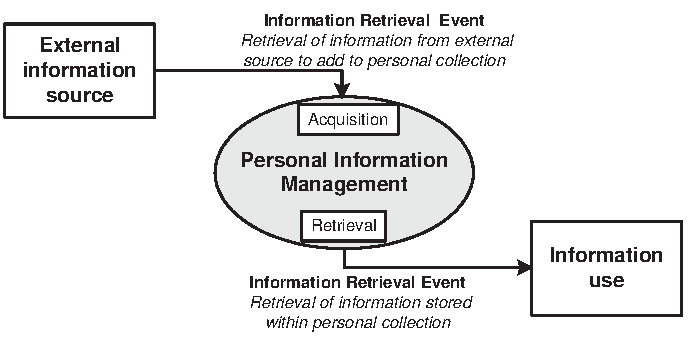
\includegraphics[height=4cm]{pictures/bg/BG-RshipPIMandIR.pdf}
	\end{center}
	\caption{The relationship between PIM and Information Retrieval}
	\label{fig:chapter2_pim_and_ir} 
\end{figure}

% LINK to \textbf{Section~\ref{bg:pim-tools}} 
% The next section moves on to consider the software tools which allow computer users to manage collections of personal information.

%%%%%%%%%%%%%%%%%%%%%%%%%%%
%%%%%%%%%%%%%%%%%%%%%%%%%%%
%%%%%%%%%%%%%%%%%%%%%%%%%%%
%%%%%%%%%%%%%%%%%%%%%%%%%%%

\newpage
%%%%%%%%%%%%%%%%%%%%%%%%%%%%%%%%%%%%%%%%%%%%%%%%%%%%%%%
\section{Personal Information Management Tools}
\label{bg:pim-tools}
%%%%%%%%%%%%%%%%%%%%%%%%%%%%%%%%%%%%%%%%%%%%%%%%%%%%%
%%%%%%%%%%%%%%%%%%%%%%%%%%%%%%%%%%%%%%%%%%%%%%%%%%%%%%
%% Consider PIM tools in terms of artifact theory
%%%%%%%%%%%%%%%%%%%%%%%%%%%%%%%%%%%%%%%%%%%%%%%%%%%%%%
%% Complex artifacts to reflect nature of PIM.  Myriad features and claims in Carroll's language. Think about the implicit theories that they manifest, although not explicitly expressed in these terms can be interpreted
%%%%%%%%%%%%%%%%%%%%%%%%%%%%%%%%%%%%%%%%%%%%%%%%%%%%%%
%% Dix: artefacts embody theories (Carroll), experiences, assumptions
%%%%%%%%%%%%%%%%%%%%%%%%%%%%%%%%%%%%%%%%%%%%%%%%%%%%%%
%% Can we consider as part of HCI knowledge
%%%%%%%%%%%%%%%%%%%%%%%%%%%%%%%%%%%%%%%%%%%%%%%%%%%%%%
%% Consider as environments rather than tools
%%%%%%%%%%%%%%%%%%%%%%%%%%%%%%%%%%%%%%%%%%%%%%%%%%%%%%

% IMPLICIT/EXPLICIT
% However they may also be performed automatically by the system. 
% Indeed, the four above sub-activities may also be \textit{implicit}, performed automatically by the system. Examples are provided in the context of the organizing sub-activity. An example of explicit organization would be the manual placement of a file within a folder. An example of implicit organization would be the default alphabetical ordering of items based on metadata that has been automatically assigned.  

% \textbf{Section~\ref{bg:pim}} discussed personal information management as an activity performed by individual computer users. This section moves on to consider the software tools that support this activity. 
%% NB: PIM-tool = complex artifact
%% PIM system = PIM-tool + managed collection
%% Defined by the primary technolgical format which it exists to manage

% The previous section presented the view of PIM taken up in this thesis, as a fundamental aspect of computer-based activity.
This section considers the software tools that allow users to manage personal information.  Firstly,
\textbf{Section~\ref{bg:pimtool-defn}} offers the term PIM-tool to designate such software.  Then, \textbf{Section~\ref{bg:pim-history}} discusses the origins of PIM-tool software.  \textbf{Section~\ref{bg:current-survey}} surveys current PIM-tool technology, and highlights the reliance on the folder hierarchy.
% It is observed that many tools such as the personal file system, email tool and web bookmark collection are based on the folder hierarchy. An abstract model of a hierarchy-based PIM-tool is presented.
\textbf{Section~\ref{bg:trends}} outlines ongoing trends in PIM-tool design. Finally, \textbf{Section~\ref{bg:integration}} considers the provision of integration between PIM-tools.




%%%%%%%%%%%%%%%%%%%%%%%%%%%
%%%%%%%%%%%%%%%%%%%%%%%%%%%
%%%%%%%%%%%%%%%%%%%%%%%%%%%
%%%%%%%%%%%%%%%%%%%%%%%%%%%

%%%%%%%%%%%%%%%%%%%%%%%%%%
\subsection{Definition}
\label{bg:pimtool-defn}
%%%%%%%%%%%%%%%%%%%%%%%%%%

A \textit{Personal Information Management tool} (abbreviated to \textit{PIM-tool} henceforth) is defined as a software tool that allows a user to manage a collection of personal information items.  The PIM-tool interface defines how a user views and interacts with the collection.  \textbf{Figure~\ref{fig:abstract_pim_tool}} illustrates the core functionality provided by a PIM-tool, consisting of support for the four PIM sub-activities outlined in \textbf{Section~\ref{bg:pim-activity-cf}}:
\begin{enumerate}
\item \textit{Support for acquisition} -- a mechanism to add items of information into a collection
\item \textit{Support for organization} -- a mechanism to arrange items within the collection. %, such as a folder hierahc % (optional) %% order, classify, structure
\item \textit{Support for maintenance} -- for example, a mechanism to remove items from a collection % (optional). % THIS IS NOT OPTIONAL
\item \textit{Support for retrieval} -- a mechanism to access items from the collection, via browsing, sorting or searching. %  (view collection, sort, browse, search, and view item)
% Two main types of explicit organization mechanism exist -- those based on browsing and those based on search
%% need examples on these!
\end{enumerate}	
%% Based on the definition of personal information management above, a PIM-tool therefore allows a user to acquire items of information, organize the collected items, maintain the collection (e.g. delete or archive items), and subsequently access items. 

% %%%%%%%%%%%%%%%%%%%%%%%%%%%%%
% FIGURE - An abstract PIM tool}
% %%%%%%%%%%%%%%%%%%%%%%%%%%%%%
\begin{figure}[hbtp]
	\begin{center}
		\leavevmode
		\includegraphics{pictures/bg/BG-AbstractPIMTool.pdf}
		\caption{An abstract PIM-tool}
		\label{fig:abstract_pim_tool}
	\end{center}
\end{figure}

PIM-tools typically support the management of personal information in a particular technological format.  Example PIM-tools in the context of a desktop computer include the file system, email reader and web browser, which are used to manage collections of files, email and web bookmarks respectively.  
% Typically the information created in such tools are stored in a collection of personal information managed within distinct tool. For example text documents produced in an editor are managed in the file system.
%%%%%%%%%%%%%%%%%%%%%%%%%%%%
% VARY IN ACTIVITY SUPPORT
%%%%%%%%%%%%%%%%%%%%%%%%%%%%
%% Question is all the above functionality compulsory?
% Note that PIM-tools differ in the extent to which they support these four sub-activities.  
PIM-tools vary significantly in the extent to which they support the four sub-activities, and how they provide that support.  Example PIM-tools are discussed in more detail in \textbf{Section~\ref{bg:current-survey}}.  As a minimum, a PIM-tool must provide mechanisms to both add items to a collection, and to retrieve them.

%%%%%%%%%%%%%%%
% NOT EDITING
%%%%%%%%%%%%%%%
The definition of PIM used in this thesis does not include the updating of items. Therefore, functionality for editing items is not considered essential for a PIM-tool. % tools used to create information such as editors are not considered as PIM-tools

%%%%%%%%%%%%%%%%%%%%%%%%%%%%%%%
% APPLICATION DOES NOT EQUAL PIM-TOOL  
%%%%%%%%%%%%%%%%%%%%%%%%%%%%%%%
There is not necessarily a one-to-one mapping from PIM-tool functionality to software applications. For example, simple email applications provide both PIM-tool functionality as defined above and also editing functionality. 
%%%%%%%%%%%%%%%%%%%%%%%
%% Application suites
%%%%%%%%%%%%%%%%%%%%%%%
In the extreme, some software applications may provide support for the management of multiple collections of personal information. For example MS-Outlook allows the user to manage no less than six types of information: email, tasks (to do-items), calendar entries, contacts, diary entries and notes. In this thesis the functionality dedicated to each type of personal information is considered a distinct PIM-tool. From this view applications such as MS-Outlook are best described as \textit{application suites} consisting of multiple PIM-tools


%%%%%%%%%%%%%%%%%%%%%%%%%%%%%%%%%%%%%
% PRIMARY/SECONDARY FUNCTION
%%%%%%%%%%%%%%%%%%%%%%%%%%%%%%%%%%%%%
% History Mechanism in Microsoft Word (example of PIM-tool functionality within the context of a larger application)
Two types of PIM-tool can be identified depending on whether PIM is a primary or secondary function:
\begin{enumerate}

\item \textit{Tools where PIM is their primary function} -- Examples of this type include the file system and contact managers.  Their main function is to facilitate the management of some collection of personal information.

\item \textit{Tools where PIM is a secondary function} -- Examples of this type include email tools which are primarily dedicated to providing a means of asynchronous communication between people.  However, they also allow the user to build a collection of electronic messages -- arguably, a secondary function.  Many modern productivity applications sometimes have secondary functionality which may be considered as a PIM-tool. For instance, the file-history mechanism in MS-Word can be considered to be a collection of items (each a reference to an edited document), which are acquired automatically based on application history.
% and the support they offer for each sub-activity are discussed.}.
Therefore, MS-Word as a whole is not a PIM-tool but it contains sub-functionality which may be considered as one.
%%%%%%%%%%%%%%%%%%%%%
% EXPLICIT/IMPLICIT
%%%%%%%%%%%%%%%%%%%%%
Note that this example also illustrates that the performance of each PIM sub-activity may be \textit{implicit} (performed automatically by the tool) or \textit{explicit} (performed by the user).
\end{enumerate}
In this thesis the term PIM-tool is used to refer to any software application that facilitates the management of personal information, regardless of whether that is its main function or not.



%%%%%%%%%%%
% Linkage
%%%%%%%%%%%
% \textbf{Section~\ref{bg:pim-history}} provides some historical context, before \textbf{Section~\ref{bg:current-survey}} surveys current PIM-tool technology.

%%%%%%%%%%%%%%%%%%%%%%%%%%%
%%%%%%%%%%%%%%%%%%%%%%%%%%%
%%%%%%%%%%%%%%%%%%%%%%%%%%%
%%%%%%%%%%%%%%%%%%%%%%%%%%%

%%%%%%%%%%%%%%%%%%%%%%%%%%%%%%%%%%%%%%%%%%%%%%%%%%%%%%%%%%%%%
\subsection{Historical Context}
\label{bg:pim-history}
%%%%%%%%%%%%%%%%%%%%%%%%%%%%%%%%%%%%%%%%%%%%%%%%%%%%%%%%%%%%%

% The roots of today's PIM-tools can be traced back to the earliest predictions of personal computing in the 1940s. 
%Bush's ideas had a huge influence on much of the subsequent development of personal computing.
%% However it was not until the 1960s that 
%%  \item \textbf{Early predictions} -- \textit{THINK: a shift from pure computation to an environment} �- Memex [Bush, 1991], Linklider
%% Man-Computer Symbiosis (1960) 
%% Multi-user systems
The evolution of today's PIM-tool technology can be traced back far beyond the first practical personal computers.  The \textit{Memex} system~\citep{bush:45} is often cited as a foresightful prediction of hypertext, envisioned using the technology of the 1940s.  Bush outlined a system where a user could archive vast amounts of microfiche material, annotate items, and create links between specific items.  The Memex system can thus be considered to encompass an early PIM-tool specification based on the acquisition of articles into a personal collection, demarcated by the links set up by the user.

In the 1960s and 70s two areas of work laid the groundwork for realizing today's PIM-tools: (1) mainframes that provided the first personal file storage, and (2) the first personal computers.

%%%%%%%%%%%%%%%%%%%%%%%%%%%%%%%%%%%%%%%%
\subsubsection{Personal space on multi-user systems}
%%%%%%%%%%%%%%%%%%%%%%%%%%%%%%%%%%%%%%%%

%%%%%%%%%%%%%%%%%%%%%%
% Early preduictions
% Time-sharing -> Multics -> UNIX
%%%%%%%%%%%%%%%%%%%%%%
%Early computers were complex monolithic machines that filled the basements of academic departments.
% far removed from today's desktop computers
% The earliest basement-filling mainframes seem a long way from today's PIM-tools.However
The first personal file storage was provided in early multi-user time-sharing computers.  The \textit{Compatible Time-sharing System (CTSS)}, developed in Project MAC at MIT, was the first mainframe to provide personal storage space to its users~\citep{ctss:62}. \textit{CTSS} users were each allocated a private tape on which to store the programs they were developing. Previous systems only provided storage for generic programs and data. 

% MULTICS
% \textit{Multics} was the first system to provide a hierarchical file system. Individual users were provided with a personal directory within which their personal files could be stored.
% offer users the facility to create a hierarchy of directories within which personal files could be stored.
The \textit{CTSS} project was the direct predecessor of the \textit{Multics} operating system, a collaboration between Bell Telephone Labs, MIT and General Electric~\citep{multics:65}.  \textit{Multics} was the first system to implement a hierarchical file system for storing data.  Users were each allocated a personal directory within the main file system.  The command-line programs that allowed users to navigate the file hierarchy will be familiar to users of DOS and other command-line shells. They included \textit{ls} to list the files in a directory, \textit{pwd} to print the current working directory, and \textit{cwd} to change the current directory.
% and UNIX
Due to development problems, Bell left the \textit{Multics} consortium and proceeded to develop an alternative operating system called \textit{UNIX}~\citep{ritchie:74}. \textit{UNIX} also offered its users a personal storage area called a \textit{home directory}, and a set of command-line utilities for accessing them.  Note that the early versions of UNIX were a long way in usability terms from today's systems.  For example the entire system had to be rebooted every time the user wanted to create a new directory!
%  Furthermore, UNIX also allowed users to create a personal hierarchy of directories to organize files
  % UNIX soon outstripped its rivals and was adopted by academic institutions around the world. 
 % Email was also pioneered on \textit{UNIX}, allowing users to store personal archives of email.
%% http://www.multicians.org/unix.html
%% 	\item Library systems allowing storing of personal bibliographies
%% the first personal computers and the desktop metaphor

The directory hierarchy\footnote{Nowadays, the directory hierarchy is also commonly referred to as the folder hierarchy, a term that was driven by the Desktop Metaphor introduced in the \textit{Xerox Star}.}, as first implemented in these multi-user systems, remains the standard mechanism for organizing items provided by PIM-tools today.

%%%%%%%%%%%%%%%%%%%%%%%%%%%%%%%%%%%%%%%%%%%
\subsubsection{The first personal computers}
%%%%%%%%%%%%%%%%%%%%%%%%%%%%%%%%%%%%%%%%%%%
% Engelbart
% Sutherland - Sketchpad
% Kay - Dynabook
% Xerox - Star
% Engelbart was driven to investigate the potential of desktop computers to augment other aspects of human activity such as managing archives of personal information.
%% What did Engelbart's system offer in terms of personal information management
A parallel thread of research lead to the first \textit{single-user personal computers}.  Early pioneers included Douglas Engelbart, who lead the research team that developed the mouse and many aspects of the graphical user interfaces (e.g.  multiple windows). Engelbart was heavily influenced by the ideas of Bush in envisioning the potential of computing technology to \textit{augment} personal activities, rather than simply to provide raw number-crunching power~\citep{engelbart:62}. 

%%%%%%%%%%
% ALTO
%%%%%%%%%%
% http://members.fortunecity.com/pcmuseum/alto.html
Further progress in hardware and graphics technology lead in 1973 to the first desktop-sized personal computer, the \textit{Xerox Alto}~\citep{wadlow:81}.  The \textit{Alto} provided the first graphical \textit{direct manipulation} alternative to the command line interfaces that had been previously used for managing files. The Alto's \textit{Neptune directory manager} provided a graphical representation of the file system, allowing files to be accessed, deleted and moved with the mouse.

%% check this is true -- re Engelbart's system
%% Check Alto re: the desktop metaphor
In 1981, the \textit{Xerox Star} was the first commercial implementation of the \textit{Desktop Metaphor}, in which the file system was mapped onto a five-level physical metaphor consisting of cabinet, drawer, hanging, manilla envelope folders, and documents~\citep{smith:82}. Cabinets, drawers, hangings and folders provided a hierarchical storage mechanism in which documents (files), created by applications such as word processors, could be filed. Users were also able to arrange document files \textit{spatially} as icons on the desktop.  Although unsuccessful commercially, the \textit{Star} was revolutionary in introducing the Desktop Metaphor, which was subsequently used in the more successful Apple II, and most subsequent personal operating systems.
% Although unsuccessful commercially, the Star development team introduced many 
% implementation of the desktop metaphor, although the first \textit{commercially successful} personal computer was the Apple II.
% Like the Alto, these desktop personal computers allowed a user to store information as files within the file system, represented graphically as folders (graphical equivalents to command-line directories), and also as icons on the desktop. 

The personal file system and desktop, as pioneered by these early personal computers, still provide the foundational PIM mechanism in today's computers.  Note that the Desktop Metaphor did not replace the command line interface, but instead augmented it.  The command line interface has been remarkably resilient, and still exists as an alternative to graphical interfaces in today's operating systems such as Windows, MacOS and Linux.  % The command-line and desktop/graphical interfaces provide alternative access mechanisms to the same underlying storage on disk.
%% The work on the Desktop Metaphor in the late 70s (see Smith et al. 1982) is attributed for the invention of the visual direct-manipulation folder hierarchy (based on the five-levels of cabinet-drawer-hanging-manila-document in the typical office file cabinet). However personal file systems based on directories accessed via the command-line a command-line were used as early as the influential 1960s Multics operating system (Multicians website, 2001). 


%%%%%%%%%%%%%%%%%%%%%%%%%%%
%%%%%%%%%%%%%%%%%%%%%%%%%%%
%%%%%%%%%%%%%%%%%%%%%%%%%%%
%%%%%%%%%%%%%%%%%%%%%%%%%%%

%%%%%%%%%%%%%%%%%%%%%%%%%%%%%%%%%%%%%%%%%%%%%%%%%%%%%%%%%%
\subsection{Contemporary PIM-tools}
\label{bg:current-survey}
%%%%%%%%%%%%%%%%%%%%%%%%%%%%%%%%%%%%%%%%%%%%%%%%%%%%%%%%%%
%% Review standard tools ONLY
%% OneNote
%% Web-based PIM-tools
%%%%%%%%%%%%%%%%%%%%%%%%%%%%%%%%%%%%%%%%%%%%%%%%%%%%%%%%%%
This section surveys contemporary PIM-tool technology.
% A model of a typical the personal information environment is proposed,
% along with a survey of common desktop PIM-tools.
Note that the focus here is on tools in use by the general public. Research prototypes that have yet to enter the public domain are considered in \textbf{Chapter~\ref{chapter:review}}.  % Ongoing trends in the design and functionality of PIM interfaces are identified in the next section, \textbf{Section~\ref{bg:trends}}.
This thesis focuses on the PIM-tools employed to manage personal information on a personal computer, as surveyed in the next section.

% The next section presents an overview of current support for personal information management that has evolved in this incremental manner.
%%%%%%%%%%%%%%%%%%%%%%%%%%%%%%%%%%%%%%%%%
%% End of history - cue current tools
%%%%%%%%%%%%%%%%%%%%%%%%%%%%%%%%%%%%%%%%%

%%%%%%%%%%%%%%%%%%%%%%%%%%%%%%%%%%%%%%%%%%%%%%%%%%%%%%
\subsubsection{Survey of desktop PIM-tools}
\label{bg:desktop-pim-tools}
%%%%%%%%%%%%%%%%%%%%%%%%%%%%%%%%%%%%%%%%%%%%%%%%%%%%%%
% Personal Information Management (PIM) is a key application domain of software technology.
%%  Need to substantiate this claim (evidence: widespread usage)
% Today's computing environments contain a wide range of PIM-tools that allow an individual to manage information in a range of technological formats such as email messages, web bookmarks, files, calendar entries, contacts.
%% THINK: add a complete survey


%%%%%%%%%%%%%%%%%%%%%%%%%%%%%%%%%%%%%%%%%%%%%%%%%%%%%%%%
% \subsubsection{Evolution of multiple PIM-tools}
%%%%%%%%%%%%%%%%%%%%%%%%%%%%%%%%%%%%%%%%%%%%%%%%%%%%%%%%
% Through the 80s and 90s, a number of PIM-tools have been developed that allow the users to manage other collections of personal information separately from the file system and desktop.
% Examples include the calendar, the address book, and with the availability of networking -- email, and the web browser.  Each of these applications has PIM-tool functionality that allows the user to manage a collection of personal information in a specialized technological format, separate to the file system.
Early personal computers were centred on managing information on the file system and on the desktop.  Since then, a number of software applications have been developed that enable users to manage distinct collections of personal information based on specialized technological formats.  Each new collection, although stored on the file system, was accessed via a dedicated PIM-tool interface.  Examples include email, originally invented on UNIX in the 1970s, and web bookmarks, introduced with the invention of the World Wide Web in the 1990s.

% 
Typical PIM-tools on a modern desktop computer include:

\begin{itemize}

%%%%%%%%%%%%%%%%%%%%%%%%%%%%%%%%%%%%%
% \subsubsection{Personal file system}
%%%%%%%%%%%%%%%%%%%%%%%%%%%%%%%%%%%%%
%% NB: this may be changing
% Acquisition is typically performed explicitly by the user as and when they save files within the hierarchy.
% Organization is both explicit and implicit. Explicit organization is based on metadata assigned to a file by the user such as name and the categorization of the file within a folder or the placement of an iconic-representation of the file at a location on the desktop.
% Maintenance support is typically explicit, it is up to the user to decide when to delete, move or archive files. Modern operating systems may also provide automatic means of performing aspects of maintenance such as synchronization or archiving. Alternatively such functionality may be provided by add-on applications.
% Retrieval from personal file systems is explicit, the user can browse for files, by navigating through the folder hierarchy, or search for files using a search tool. Some operating systems also provide implicit retrieval facilities such as history-based mechanisms.
\item \textit{Personal file system} --  The personal file system is defined as the portions of the file system used to store personal document files. Operating systems typically provide a default area for this purpose such as ``My Documents'' in Microsoft Windows, or the ``home directory'' in UNIX.
%% PIM-tool functionality within the operating system
Files can be created in a range of formats (e.g. text document, spreadsheet, presentation) depending on the application used to create and view the file. Since files of different formats are managed together in the personal file system, they are treated as members of the same collection of personal information.  %The current generation of personal file systems, such as those found in Microsoft Windows, MacOS and UNIX are based on a folder hierarchy.

% Key examples include the email tool for managing electronic messages, the calendar, the to-do list and the web bookmark tool within a web browser.  
Most other PIM-tools are limited to managing a collection of information in a particular technological format. Although such collections are stored on the file system, they are accessed using a different interface.

%%%%%%%%%%%%%%%%%%%%%%%%%%%%%%%%%%%%%
% \subsubsection{Email tool}
%%%%%%%%%%%%%%%%%%%%%%%%%%%%%%%%%%%%%
% Primary purpose = communication + secondary PIM	
% Email PIM-tool functionality is also based on the folder hierarchy.
% Acquisition is implicit. Email messages are acquired automatically into a folder called the Inbox. Both explicit and implicit organizational mechanisms are provided. Explicit organization is based on the categorization of emails within folders. Mechanisms may also exist to label emails with metadata such as an important flag. Such metadata is considered an organizational mechanism since it allows emails to be ordered based on that piece of metadata. Implicit organization performed by the system is based on the assignment of implicit metadata such as date received, author and size. Filters set up by the user can also be used to automatically organize emails as they arrive. Maintenance facilities are similar to those of the personal file system, although exact functionality varies between tools. As well as explicit maintenance performed by the user, email tools may provide automatic archiving mechanisms. Retrieval is explicit based on browsing or searching.
% Email tool facility for managing electronic messages (typical of PIM-tools based on hierarchical folder-based organization)
\item \textit{The email tool used to manage electronic messages} -- Note that email messages may contain attached files such as text documents, or embedded web addresses. Thus the email PIM-tool, although its primary technological format is the email message, is often used to manage information of other formats.

%%%%%%%%%%%%%%%%%%%%%%%%%%%%%%%%%%%%%%%%%%%%%%%%%%%%%%%%%%%%%%%
% \subsubsection{Web browser facility for managing bookmarks}
%%%%%%%%%%%%%%%%%%%%%%%%%%%%%%%%%%%%%%%%%%%%%%%%%%%%%%%%%%%%%%%
% Primary purpose = information retrieval + secondary PIM
\item \textit{The web bookmark management mechanism located within a web browser} -- The key difference between the bookmark PIM-tool and other tools such as email is the nature of the items managed within. Bookmarks do not contain user-defined content, they are instead \textit{references} to pages stored on remote websites.
%% AKA pointers or addresses

Both the web bookmark and email PIM-tools provide a hierarchical organizing mechanism dedicated to the respective technological format. 

%%%%%%%%%%%%%%%%%%%%%%%%%%%%%%%%%%%%%
% \subsubsection{Calendar}
%%%%%%%%%%%%%%%%%%%%%%%%%%%%%%%%%%%%%
% Calendar for managing appointments (example of an PIM-tool based on implicit organization)
\item \textit{Calendar} -- The calendar is representative of PIM-tools which are not based on a hierarchical organizing mechanism. Managed items are appointments which are ordered within the implicit chronological organizational scheme provided by the calendar software.

% \item \textit{Other PIM-tools} -- 
 
\end{itemize}

Other common PIM-tools include to-do lists, reference managers, image collections, music collections, and contact managers.
% In the following examples a focus is taken on graphical/direct-manipulation interfaces since these are more commonly used relative to command-line interfaces. In addition details relative to specific implementations on particular operating systems are abstracted, instead general PIM-tool functionality is considered.
%%
%% \textbf{Interface technology

% As well as an increase in the number of PIM-tools on personal computers, there has also been a trend towards the management of information on multiple computing devices such as websites on remote computers, mobile phones and PDA devices.  Although these two trends have resulted in a wide range of powerful functionality for users (more PIM-tools on more devices), they have also contributed to the problems of fragmentation in today's personal information environment.
%% \textit{Provide detail on:
%% \begin{itemize}
%% \item First email allowing user to store messages, 1970s -- early intranet (collection of email)
%% \item NCSA Mosaic by Marc Andreessen and Eric Bina allowing web bookmarking, 1993 %%(collection of web bookmarks)
%% \end{itemize}}
It can be observed that the fundamental design of PIM-tools has changed relatively little since the invention of the hierarchical file system, and the Desktop Metaphor.  Although users have been offered the ability to manage many new types of personal information (e.g. email), the interfaces are still based on the same underlying mechanisms~\citep{Cooper:03}.  % The next section considers the most common organizational mechanism, that of the folder or directory hierarchy.



%%%%%%%%%%%%%%%%%%%%%%%%%%%
%%%%%%%%%%%%%%%%%%%%%%%%%%%
%%%%%%%%%%%%%%%%%%%%%%%%%%%
%%%%%%%%%%%%%%%%%%%%%%%%%%%

%%%%%%%%%%%%%%%%%%%%%%%%%%%%%%%%%%%%%%%%%%%%%%%%%%%%%%%%%%%
\subsubsection{Hierarchy-based PIM-tools}
\label{bg:pimtool-cf}
%%%%%%%%%%%%%%%%%%%%%%%%%%%%%%%%%%%%%%%%%%%%%%%%%%%%%%%%%%%
% Users may create semantic or spatial categories

% \textbf{Section~\ref{bg:pimtool-cf}} presents a second conceptual framework, representing a canonical hierarchy-based PIM-tool. The framework defines concepts and terminology used throughout the remainder of the thesis. Section~\ref{bg:hierarchy-model} outlines an abstract model of the functionality afforded by a hierarchy-based PIM-tool.
% Although there is some variance in low-level features and interface design, the tools for organizing  document files, email, and web bookmarks are remarkably similar: they are all founded on the folder hierarchy.
The folder hierarchy is the standard mechanism for organizing collections of personal information~\citep{dourish:99a}.  It allows the user to create a personal classification scheme. The user may choose to create categories based on whichever organisational dimensions  that they see as relevant (e.g. role, project or time).  Studies of classificatory behaviour are reported in \textbf{Section~\ref{review:pim-empirical-review}}.

% The folder hierarchy is referred to as the directory tree in UNIX.

%%
%% Foundational PIM-organizing mechanism = hierarchy + metadata
%% \textbf{Hierarchy as uber-PIM organizing mechanism}
%% Theory underlying the design of PIM interfaces is discussed.

%%%%%%%%%%%%%%%%%%%%%%%%%%%%%%%%%%%%%%%%%%%%%%%%%%%%
% \subsubsection{Classification Schemes}
%%%%%%%%%%%%%%%%%%%%%%%%%%%%%%%%%%%%%%%%%%%%%%%%%%%%
%% Hierarchy as a cognitive artefact, classification scheme, concept map, scaffolding (cognitive economy and perceived world structure).
%% Personal CS cf. infrastructural. Cultural bias.

% The  a personal classification scheme allows the user to create an individualised organization, customized to their way of thinking and working.   % Categories can be represented in various ways, depending on the classificatory mechanism in use.  A typical desktop workspace might contain categories in the form of a cluster of icons at a spatial location, emails contained within a folder labelled semantically with a text string, or a set of hypertext links on a personal web page. 

% Our electronic workspaces contain a wide range of personal classification schemes. Common examples in desktop workspace include the folder hierarchies of the file system, mail tools and web browsers for organising documents, messages and web links respectively. Many software packages also contain their own specific hierarchies for organising specialized types of information such as source code, images and music files. Some operating systems contain their own idiosyncratic hierarchies, such as the Start Menu of Microsoft Windows that is used to organise software tools and access recently accessed documents. 

% SPATIAL ORGANZING TO PLACE Resources may also be organized spatially as an arrangement of icons on the desktop.  Workspace itself may be organized in terms of virtual windows assigned to a flat category space~\citep{rooms:86}.


%% CHECK SECTION NUMBER
%%%%%%%%%%%%%%%%%%%%%%%%%%%%%%%%%%%%%%%%%%%%%%%%%%%%%
%\subsubsection{Model of a hierarchy-based PIM tool}
% \label{bg:hierarchy-model}
%%%%%%%%%%%%%%%%%%%%%%%%%%%%%%%%%%%%%%%%%%%%%%%%%%%%%

\textbf{Figure~\ref{fig:abstract_pim_tool_with_hierarchy}} shows a simple model of a hierarchy-based PIM tool.  Hierarchy-based PIM tools support the four PIM sub-activities as follows:

% %%%%%%%%%%%%%%%%%%%%%%%%%%%%%
% FIGURE - The core PIM functionality present in
% document file managers, email managers, and web browsers}
% %%%%%%%%%%%%%%%%%%%%%%%%%%%%%
\begin{figure}[hbtp]
	\begin{center}
		\leavevmode
		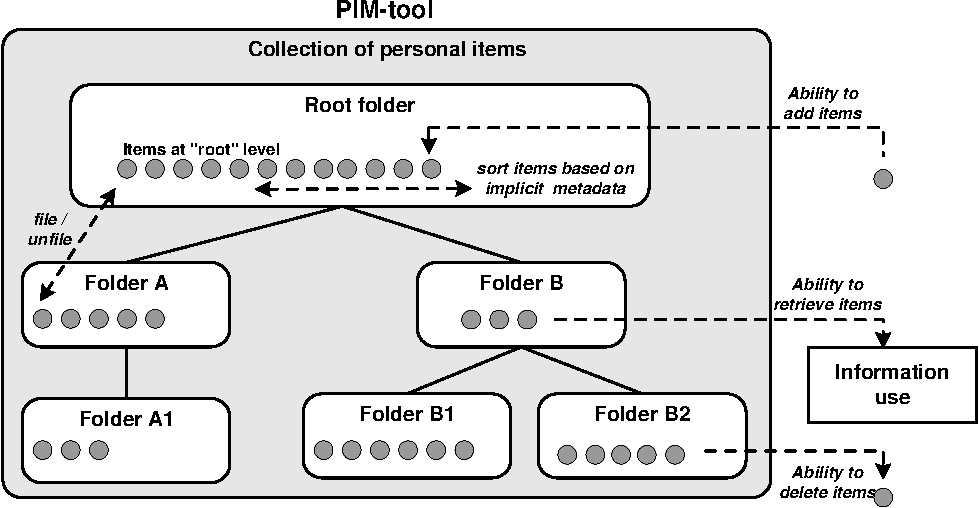
\includegraphics[height=6cm]{pictures/bg/BG-AbstractPimToolWithHierarchy.pdf}
		\caption{Model of a hierarchy-based PIM-tool}
		\label{fig:abstract_pim_tool_with_hierarchy}
	\end{center}
\end{figure}
%% Each item must also possess an index or label via which it can be accessed. Indices may be based on an explicit name (e.g. a filename) or implicit metadata (e.g. the subject line of an email).

\begin{itemize} % The user is enabled to manage items within an unfiled list at the ``top-level'', and within a hierarchy of folders.
\item \textit{Acquisition} -- items may be added as unfiled items in the top-level ``root'' folder, or placed directly into a low-level folder. 
%% ITEMS Can have implicit or explicit metadata. There may also be the potential to assign explicit metadata (e.g. name) to items.
%% items: minimum organizational unit

\item \textit{Organization} -- Explicit organization is enabled through the placement of items within folders. The user may change the folder structure by adding new folders, or renaming, deleting or moving existing folders.
% Implicit organization is carried out by the automatic assignment of implicit metadata such as size and date-created.
Typically, items are limited to placement in one folder location.  However, some folder hierarchy implementations allow the user to set-up \textit{links} or \textit{short-cuts} which can act as references from multiple locations to a particular item.

\item \textit{Maintenance} -- Typically, PIM-tools provide a mechanism to delete items. Implicit or explicit means of archiving may also be provided.

\item \textit{Retrieval} -- PIM-tools typically provide the ability to retrieve items from the collection through a combination of mechanisms. Firstly, users may browse through the hierarchy to retrieve items.  Two types of browsing can be highlighted: (1) browsing of folders, using user-defined explicit ``location'' metadata encoded in the folder structure; and (2) sorting/scanning of items within a folder, ordered by user-defined metadata (e.g. ``name'') or implicit metadata (e.g. ``date created''). The PIM-tool may also offer a search facility. Retrieved items may be re-saved within the hierarchy after editing.
% a sorting mechanism allows the user to order items in terms of their implicit metadata (e.g. date-created) or explicit metadata (e.g. name).  add types of browsing from CHI paper

\end{itemize}

Two types of interface are commonly employed to manage hierarchies: (1) a direct-manipulation file manager (pioneered in the Xerox Alto Neptune file manager~\citep{wadlow:81}), and (2) the command-line tools of UNIX or DOS. 

\textbf{Section~\ref{review:pim-theory-review}} surveys theory relating to PIM, including arguments in favour and against the use of hierarchical organization.



%%%%%%%%%%%%%%%%%%%%%%%%%%%
%%%%%%%%%%%%%%%%%%%%%%%%%%%
%%%%%%%%%%%%%%%%%%%%%%%%%%%
%%%%%%%%%%%%%%%%%%%%%%%%%%%

%%%%%%%%%%%%%%%%%%%%%%%%%%%%%%%%%%%%%%%%%%%%%%%%%%%%%%
\subsubsection{The Personal Information Environment}
\label{bg:pie}
%%%%%%%%%%%%%%%%%%%%%%%%%%%%%%%%%%%%%%%%%%%%%%%%%%%%%%
%% AKA workspace, activity space (Kirsh)

%%%%%%%%%%%%%%%%%%%%%%%%%%%
% PIE = physical + digital
%%%%%%%%%%%%%%%%%%%%%%%%%%%
The \textit{personal information environment} is defined as the aggregate of all collections of personal information. \textbf{Figure~\ref{fig:chapter2_pie}} offers a graphical summary of a personal information environment encompassing both the physical and digital domains.
%%%%%%%%%%%%%%%%%%%%%%%%
% FOCUS: digital PIE
%%%%%%%%%%%%%%%%%%%%%%%%
Note that the rest of this thesis focuses on the digital personal information environment which consists of:
% of all PIM-tools that allow an individual to manage personal information.  The personal information environment consists of the various interactive devices that allow an individual to manage personal information. These devices include:

\begin{enumerate}

\item \textit{Personal information collections stored on computers that the user has physical access to} -- Examples include desktop and laptop computers in work and home contexts.

\item \textit{Personal information collections stored on remote computers} -- As well as storing information on their local computer, the user may store information remotely on network drives.  Furthermore, many internet websites are now providing PIM-tool technology. Examples include web-based PIM-tools include email services (e.g. MS-Hotmail), on-line document management services, on-line calendars (e.g. Yahoo Calendar!), and shopping ``wish-lists'' stored on e-commerce sites such as amazon.com.

% In recent years, mobile devices such as cellular telephones and personal digital assistants have become commonplace. In addition it is common for people to own multiple computers at work and home. Due to this variety of digital devices people now manage personal information on multiple devices.
% A third trend is that of websites providing PIM-tool functionality. On one hand, many websites provide traditional PIM-tool-like functionality such management of email or to do-items. Also many e-commerce sites and on-line applications allow the user to manage collections of personal information relating to the site content. One example of this type is the amazon.com website which allows the user to manage a ``wish list'' of books they wish to purchase.

\item \textit{Personal information collections stored on mobile devices} -- Devices such as mobile phones and personal digital assistants (PDAs) are commonly used to manage contacts and notes.

% \item Personal information in the form of recorded messages stored in voice-mail systems

\end{enumerate}



% %%%%%%%%%%%%%%%%%%%%%%%%%%%%%%%%%%%%%%%%
% FIGURE - The Personal Information Environment
% %%%%%%%%%%%%%%%%%%%%%%%%%%%%%%%%%%%%%%%%
\begin{figure}[hbtp]
	\begin{center}
		\leavevmode
		%% [height=2in, width=.9\textwidth] 
		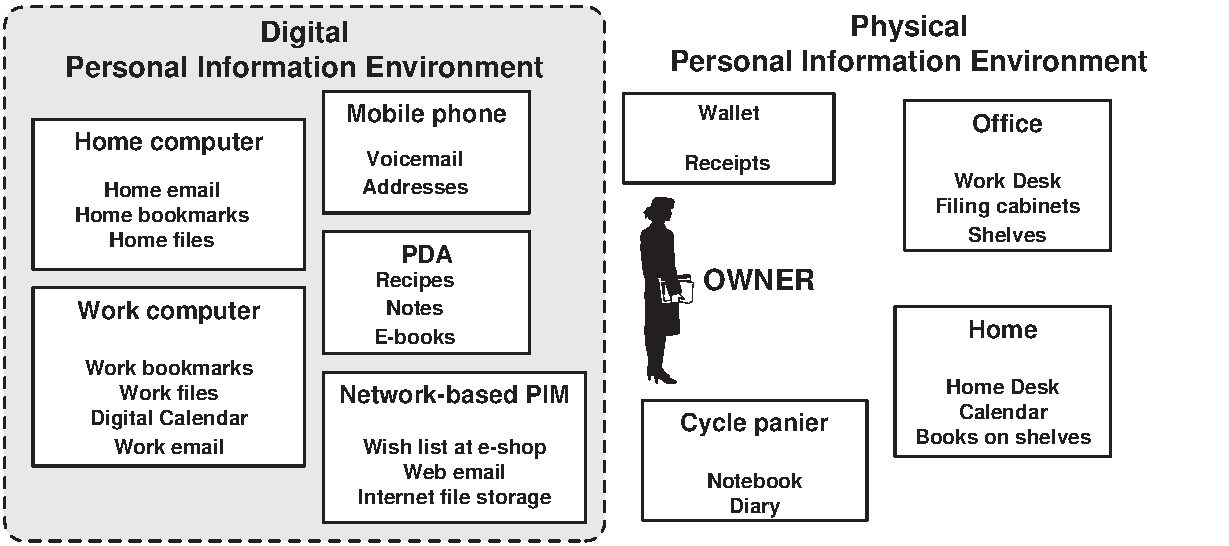
\includegraphics[width=.9\textwidth] {pictures/bg/BG-ExtendedPersonalWorkspace.pdf}
	\end{center}
	\caption{The personal information environment in both the physical and digital domains}
	\label{fig:chapter2_pie}
\end{figure}

%%%%%%%%%%%%%%%%%%%%%%%%%%%
%%%%%%%%%%%%%%%%%%%%%%%%%%%
%%%%%%%%%%%%%%%%%%%%%%%%%%%
%%%%%%%%%%%%%%%%%%%%%%%%%%%

\newpage
%%%%%%%%%%%%%%%%%%%%%%%%%%%%%%%%%%%%%%%%
\subsection{Trends in PIM-tool Design and Usage}
\label{bg:trends}
%%%%%%%%%%%%%%%%%%%%%%%%%%%%%%%%%%%%%%%%


Several ongoing trends can be identified in the design of PIM-tool technology:
\begin{enumerate}

% MORE USERS
\item \textit{Increasing numbers of users} -- With the boom in personal computing over the past decade,  millions of users now manage collections of email, files and bookmarks. Whereas in the past computer users were technically trained, today's PIM-tool users are from all walks of life and levels of technical expertise.  In other words, PIM tool technology is now a mass-market.

\item \textit{More collections of personal information} -- As noted in the previous section, today's personal information environment has evolved in a piecemeal incremental manner as new devices, PIM-tools, and technological formats have been invented.  This growth continues as more devices and websites offer PIM-tool functionality. 

%% trend/tension - bloating of tools (talk about in terms of task-artifact cycle)
%% ME: physical analogy - everyone has same desk and can paint/arrange different way. general-purpose, not designed with a specific user in mind
\item \textit{Increasing PIM-tool complexity} -- This increase in tool complexity is due to the addition of extra functionality and has been termed \textit{bloating}~\citep{mcgrenere:02}.  One reason for this phenomenon is that PIM-tools must cater for many possible approaches to managing personal information. PIM-tool developers must cater for all possible user groups -- from corporate users who depend on email during their working day, through to novice home users who may only check their email once a week. One example of the emerging complexity is that many email tools now provide integrated to-do item support. 
% A physical analogy might be millions of people sharing the same design of desk or diary. This genericity has contributed to the apparent trend towards increasing complexity in PIM-tools. 

\end{enumerate}

% These three trends -- increasing numbers of technically unsophisticated users, more collections of personal information, and   of more less technically sophisticated users, more collections and more complexity is problematic. % DISCUSS. 

%%%%%%%%%%%%%%%%%%%%%%%%%%%%%%%%%%%%%%
%% WHERE TO PLACE RESEARCH TRENDS??
%%%%%%%%%%%%%%%%%%%%%%%%%%%%%%%%%%%%%%
%% 2d/3d, speech-based systems
%% Such as 		\item Trend: increased intelligence/automation -- automation/overhead trade-off, limits of intelligent interfaces
%% 		\item Trend: Move away from the hierarchy? (see research prototypes below for more detail)
%% Move for/away from application.  No really a trend, more of a trade-off.  increasing specialization -- Tool-centric, embedding strategy/specialization strategy - Apple iApps

% \textbf{Section~\ref{bg:pie}} presents discusses the personal information environment, formed by the set of PIM-tools.
% discusses the trend towards the availability of more PIM-tools supporting the management of more types of personal information.
%% Then the trend towards increased integration is discussed in more detail in \textbf{Section~\ref{bg:integration}}.

%%%%%%%%%%%%%%%%%%%%%%%%%%%
%%%%%%%%%%%%%%%%%%%%%%%%%%%
%%%%%%%%%%%%%%%%%%%%%%%%%%%
%%%%%%%%%%%%%%%%%%%%%%%%%%%


%%%%%%%%%%%%%%%%%%%%%%%%%%%%%%%%%%%%%%%%%%%%%
\subsection{Integration between PIM-tools}
\label{bg:integration}
%%%%%%%%%%%%%%%%%%%%%%%%%%%%%%%%%%%%%%%%%%%%%
%% *********************
%% ADD: why integrate???
%% *********************
%% Application integration vs. data integration
%% hypertext-based integration
%% Mentions by Bellotti and Kaptelinin
%% Need to talk about the term `integration'?
%% Can we think about integration in terms of:
%		a) PIM tools / technological formats / collections
%		b) production activities
%		c) PIM sub-activities?
\textbf{Section~\ref{bg:pie}} described the historic trend towards multiple PIM-tools on multiple devices to form an extended personal information environment.  The provision of integration between PIM-tools is a key theme in this thesis.  This section offers a definition of integration, and surveys common integration mechanisms.
% This has lead to the need to provide integration between distinct PIM-tools.  

Although the term integration appears commonly in the marketing of PIM-tool software and other interfaces, there is no agreed definition in the research community.  The Oxford English Dictionary defines \textit{integration} as \textit{``the act or process of making whole or entire''}.  Here an integration mechanism is defined as a software component which provides user functionality that bridges two or more distinct PIM-tools.

\textbf{Figure~\ref{fig:chapter2_pim-tool_integration}} summarizes the integration mechanisms on a typical desktop computer running MS-Windows.  They are discussed as follows: % A survey of a typical Microsoft Windows machine reveals the following existing forms of integration between PIM-tools:
%% 
%% The terms integration and cross-tool defined, and current cross-tool mechanisms for integrating PIM tools are discussed.

\begin{enumerate}

\item \textit{Mechanisms that allows the user to initiate an operation in another PIM-tool} --  For example, right-clicking on an email address in an email message in MS-Outlook, allows the user to perform a search for that email address in the contact manager.
% to be taken to the address book (collection of contacts)
	
\item \textit{Mechanisms that allow information within one PIM-tool to be transferred to another PIM-tool} -- A simple example of this type is the ``cut-and-paste'' function provided by MS-Windows, e.g. copying some text from a file to an email.  Other ``higher-level'' operations combine the transfer of information with the initiation of an operation in the other PIM-tool., e.g. the ``Send-to'' mechanism allows a file to be attached within a newly created email message.
 %% send-to (example of add-on, bolt-on) (data transfer)

\item \textit{Mechanisms that allow items of various technological formats to be managed in a particular collection as ``primary-level items''} -- For example, MS-Windows allows the user to save email messages as a file within the file system. % An email saved in the file system is then equivalent to any other file.

\item \textit{Mechanisms that allow an items of various technological formats to be embedded within items of another format} -- Such embedded items are managed indirectly, via the item in which they are embedded.  An example of this type is email attachments: the ability to attach a file or bookmark within an email message. Typically, a reverse mechanism is also provided to allow the transfer of an attached item back to its native PIM-tool. % Clicking on an embedded item typically allows it to be opened within the foreign tool.

\item \textit{Retrieval mechanisms that bridge multiple tools} -- One example are cross-tool search mechanisms, e.g. SixDegrees~\citep{SixDegrees}, which allow the user to search multiple collections of information (e.g. files and email) in one operation. Some PIM-tools also permit cross-tool retrieval through browsing multiple collections. For instance MS-Windows Explorer allows the user to browse both the personal file system and the bookmark collection\footnote{The bookmark collection is stored within a special region of the MS-Windows file system in the ``Favorites'' folder.}.

\item \textit{Application suites that aggregate multiple PIM-tools} -- An example of this type is MS-Outlook which includes the PIM-tool functionality to manage five distinct collections of information: email, to-do items, notes, calendar and diary.

	% \item A final form of integration can be considered at the interface level in terms of consistency. Multiple PIM-tools often provide similar functionality such as search which are accessed via similar interfaces.
	
\end{enumerate}

% %%%%%%%%%%%%%%%%%%%%%%%%%%%%%%%%%%%%%%%%
% FIGURE - Integration between PIM-tools
% %%%%%%%%%%%%%%%%%%%%%%%%%%%%%%%%%%%%%%%%
\begin{figure}[hbtp]
	\begin{center}
		\leavevmode
		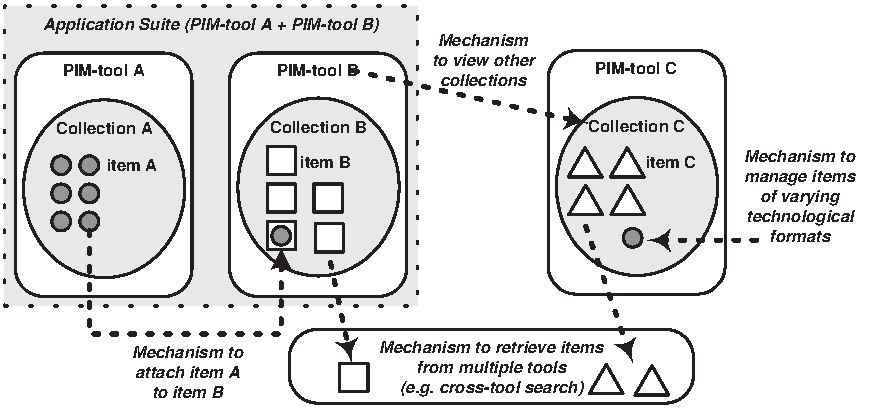
\includegraphics[height=6cm]{pictures/bg/BG-ToolIntegration.pdf}
	\end{center}
	\caption{PIM-tool integration mechanisms found in modern desktop operating systems}
	\label{fig:chapter2_pim-tool_integration}
\end{figure}

%% OTHER:
%% 
%% traversal between collections
%% All software applications are "integrated", can co-exist within the desktop graphical environment.

% It should be noted that all of these common integration approaches are effectively ``bolt-on'' mechanisms.
The range of integration mechanisms listed above is typical of most commonly available operating systems at the time of writing.  It should be noted that all of these common integration approaches are effectively ``bolt-on'' mechanisms.  Despite this wide range of integration mechanisms, information in different technological formats is managed in distinct collections within distinct PIM-tools.  

% CONTARST WITH SYNCHRONIZATION. \textit{Synchronization mechanisms that replicate items between collections of a particular technological format}. For example mirroring a work file system with one at home.  Not integration as the same technological format.

Note that this section has focused on integration available to ordinary users. Research aimed at improving integration is discussed in \textbf{Section 3.5}, including systems that unify the management of multiple types of information within a consolidated interface.
%% TODO: update section number!!
%% Simple context-aware: Nardi and co. - Data Detectors (example of research that became part of a commercial product)~\cite{bn:98}



%%%%%%%%%%%%%%%%%%%%%%%%%%%
%%%%%%%%%%%%%%%%%%%%%%%%%%%
%%%%%%%%%%%%%%%%%%%%%%%%%%%
%%%%%%%%%%%%%%%%%%%%%%%%%%%

%%%%%%%%%%%%%%%%%%%%%%%%%%%%%%%%%%
%\subsection{Summary}
%\label{bg:summary}
%%%%%%%%%%%%%%%%%%%%%%%%%%%%%%%%%%

% \textbf{Section~\ref{bg:pim-tools}} provided further conceptual background to the thesis by introducing PIM-tools. Personal computer users have access to a powerful existing set of PIM-tools allowing them to manage a range of types of information. Studies of tool usage are described in \textbf{Chapter~\ref{chapter:review}}.
%%
%% Relate to reported user problems: link towards HCI studies to follow.  Need for more design work? Users have powerful set of tools.  What is missing?

%%%%%%%%%%%%%%%%%%%%%%%%%%%
%%%%%%%%%%%%%%%%%%%%%%%%%%%
%%%%%%%%%%%%%%%%%%%%%%%%%%%
%%%%%%%%%%%%%%%%%%%%%%%%%%%

%% \newpage
%%%%%%%%%%%%%%%%%%%%%%%%%%%%%%%%%%
%%%%%%%%%%%%%%%%%%%%%%%%%%%%%%%%%%
\section{Summary}
\label{bg:conclusion}
%%%%%%%%%%%%%%%%%%%%%%%%%%%%%%%%%%
%%%%%%%%%%%%%%%%%%%%%%%%%%%%%%%%%%

% This section presents the main conclusions of \textbf{Chapter 2}.
\textbf{Section~\ref{bg:pim}} offered a conceptual framework detailing the view of PIM taken in this thesis, as  an activity consisting of four sub-activities: acquisition, organization, maintenance, and retrieval. \textbf{Section~\ref{bg:pim-tools}} defined a PIM-tool as a software component which enables the user to manage a collection of personal information. A survey of existing PIM-tool technology was also provided, along with a discussion of their evolution from early multi-user systems.
%%
%% that define key concepts and terms for discussing (1) PIM as an activity, and (2) the tools that facilitate PIM.

\textbf{Chapter~\ref{chapter:review}} moves on to review relevant research carried out within Human-Computer Interaction and other related disciplines, aimed at investigating user needs regarding PIM, and designing improved technology to support it.

%%%%%%%%%%%%%%%%%%%%%%%%%%%%%%%%%%%%%%%%%%
%% Mention relationship to other chapters:
%%%%%%%%%%%%%%%%%%%%%%%%%%%%%%%%%%%%%%%%%%
%% 
%% PIM conceptual framework developed in more depth in Chapter 4?
%% Reiterate PIM as an appication domain within HCI.
%% Now move onto next chapter: a review of previous research on PIM within HCI and related disciplines. 

%%%%%%%%%%%%%%%%%%%%%%%%%%%%%%%%%
% FIN THESIS CHAPTER 2: BACKGROUND
%%%%%%%%%%%%%%%%%%%%%%%%%%%%%%%%%
% \textit{This draft of ``Chapter 2 Background'' was printed \today}



% %%%%%%%%%%%%%%%%%%%%%%%%%%%%%

% chapter 3 - Literature Review

% %%%%%%%%%%%%%%%%%%%%%%%%%%%%%

\chapter{Literature Review}

\label{chapter:review}

% \textit{CHAPTER 3 LEFT INTENTIONALLY BLANK AS A PLACEHOLDER}


%%%%%%%%%%%%%%%%%%%%%%%%%%%%%%%%%%%%%%%%%%%%%%%%%%%%%%%%%%%%%%%%%%%%%
% Richard Boardman rick@ic.ac.uk
% PhD Thesis - Department of Electrical and Electronic Engineering
% Imperial College London SW7 2BT UK
% %%%%%%%%%%%%%%%%%%%%%%%%%%%%%%%%%%%%%%%%%%%%%%%%%%%%%%%%%%%%%%%%%%%
% Improving Tool Support for Personal Information Management
% CHAPTER 3 - LITERATURE REVIEW
% Version 25, 10th November 2003
%%%%%%%%%%%%%%%%%%%%%%%%%%%%%%%%%%%%%%%%%%%%%%%%%%%%%%%%%%%%%%%%%%%%%
%%%%%%%%%%%%
%% VOCAB
%%%%%%%%%%%%
%% Good words for review: appraise, examine, consider, assess previous work, scrutinise, acknowledge}
%% Good words for analysis: it has been argued/proposed, justify, suggest, compelling}
%% suggests that X leads to Y
%% implications for Y are discussed
%% phrase: used to argue the potential
%%%%%%%%%%%%%%%%%%%%%%%%%%%%%%%%%%%%%%%%%%%%%%%%%%%%%%%%%%%%%%%%%%%%%%%%%%%%%%%%%%%%%%
%% AIm: produce a well-thought out  criticism of:
%% a) why important
%% b) how it affected my work
%% c) present evolution of ideas in my field
%% d) how the problem addressed in this thesis relates to them
%%%%%%%%%%%%%%%%%%%%%%%%%%%%%%%%%%%%%%%%%%%%%%%%%%%%%%%%%%%%%%%%%%%%%%%%%%%%%%%%%%%%%%
%% Use CF to structure?
%% Relate sections to parts of thesis where used
%% Consider previous research in terms of quality and validity 
%%%%%%%%%%%%%%%%%%%%%%%%%%%%%%%%%%%%%%%%%%%%%%%%%%%%%%%%%%%%%%%%%%%%%%%%%%%%%%%%%%%%%%

%%%%%%%%%%%%%%%%%%%%%%%%
\section{Introduction}
\label{review-introduction}
%%%%%%%%%%%%%%%%%%%%%%%%
This chapter offers a critical review of prior research relevant to Personal Information Management (PIM). %\footnote{This draft of ``Chapter 3 Literature Review'' was printed \today}.
% Existing knowledge is surveyed from the field of Human Computer Interaction (HCI) and other related disciplines such as Information Science and Cognitive Psychology.  A particular focus is taken on Human-Computer Interaction, since this is the field to which the author seeks to contribute.
%%%%%%%%%%%%%%%%
%% ADD DISCLAIMER
%%%%%%%%%%%%%%%%
% It should be noted that the interdisciplinary nature of research, and the broad range of design in this area, plus lack of coherency means that any survey of work cannot hope to be complete. However it is hoped that a representative summary of important work is provided. 
%%%%%%%%
% AIMS
%%%%%%%%
%% link from research gap to the specific problem
%% identify areas in need of further research
%% present context of the work
%%
%% Identify research gaps which this thesis can address}
%% 
%% after stating how existing knowledge is lacking for solving this problem.
%% 
%% review concludes by attempting to provide justification/motivate/argue for my chosen methodology and contributions.
% field evidence to justify the design and methodological decisions made
%%%%%%%%%%%%%%%%%%%%%%%%%%%%%%
% Relate to overall PhD aims
%%%%%%%%%%%%%%%%%%%%%%%%%%%%%%
% The chapter offers three contributions towards the overall thesis. Firstly the chapter aims to review previous work in the field in terms of key contributions and limitations.
%%%%%%%%%%%%%%%%%%%%%%%%%%%%%%%%%%
% \subsection{Overview of Chapter}
%%%%%%%%%%%%%%%%%%%%%%%%%%%%%%%%%%
% The chapter is structured as follows.
Firstly, \textbf{Section~\ref{review:hci}} provides an overview of Human-Computer Interaction (HCI), the research field to which the thesis contributes.
% PIM is identified as an important application domain within HCI.
\textbf{Section~\ref{review:pim-research-overview}} identifies the three main types of HCI research related to PIM: empirical studies, technology prototypes, and theory development.  The next three sections deal with each area in turn.  \textbf{Section~\ref{review:pim-empirical-review}} reviews empirical work, \textbf{Section~\ref{review:pim-technological-review}} surveys PIM technology, focusing on design efforts to improve PIM-integration, and \textbf{Section~\ref{review:pim-theory-review}} reviews relevant theory.
% A second aim is to identify gaps in current knowledge where further work is required, and where this thesis can contribute.
% summarizes their main findings and discusses how they relate to one another.  The section also makes recommendations for more effective future research in the area.
% Based on this critical analysis of prior work, a research agenda will be laid out to address the identified research problem.
% A final aim is to justify the selection of methodology . This involves the surveying of methods and techniques applied to the area, as well as others that could be applied.
%  sets out a research agenda that defines the initial plan of work taken in this thesis.
% Finally \textbf{Section~\ref{review:conclusion}} summarizes the contributions of the chapter towards the overall thesis.
\textbf{Section~\ref{review:discussion}} draws together the three areas, and identifies a key research gap, the lack of empirical support for the design of PIM-integration mechanisms.  Based on this analysis, \textbf{Section~\ref{review:research-agenda}} sets out a research agenda for the thesis, and \textbf{Section~\ref{review:methodology}} justifies the selection of methodology employed in later chapters. % in the thesis.







%%%%%%%%%%%%%%%%%%%%%%%%%%%%%%%%%%%%%%%%%%%%%%%%%%%%
%%%%%%%%%%%%%%%%%%%%%%%%%%%%%%%%%%%%%%%%%%%%%%%%%%%%
\subsection{Human-Computer Interaction}
\label{review:hci}
%%%%%%%%%%%%%%%%%%%%%%%%%%%%%%%%%%%%%%%%%%%%%%%%%%%%
%%%%%%%%%%%%%%%%%%%%%%%%%%%%%%%%%%%%%%%%%%%%%%%%%%%%

%%%%%%%%%%%%%%%
% SIGNPOSTING
%%%%%%%%%%%%%%%
% This section provides an overview of Human-Computer Interaction (HCI), the research field to which the thesis contributes. The Task-Artefact cycle is presented as a framework in which HCI research and practice can be discussed. Personal information management is considered as a key application domain within HCI.

%%%%%%%%%%%%%%%%%%%
% Intro to HCI
%%%%%%%%%%%%%%%%%%%
%% Sutcliffe's framework of HCI application and technology domains is discussed. 
%% 
%% HCI is a young, interdisciplinary, applied research field containing many competing methods and research paradigms.  The chapter commences with a broad overview/sketch of the aims of HCI, its dominant research paradigms, and the various forms that HCI knowledge can take.  This overview is used to structure the remainder of the chapter focused on personal information management.
%%
%% The aim of HCI research is to provide a knowledge base to support  directed at the design of usable interactive systems~\citep{sutcliffe:00}.
%% Sutcliffe terms "`HCI-research"' as "`HCI theory"'
%% research theory versus craft-level experience/heuristics
%%  NB HCI-research can also  (those directed at research and those directed at design)
\citet{acm:96} define Human-Computer Interaction (HCI) as the \textit{``discipline concerned with the design, evaluation and implementation of interactive computing systems for human use and with the study of major phenomena surrounding them''}.
%% Two aspects of HCI exist: HCI research and HCI practice, differentiated by their end-product.
A key aim of HCI research is to provide a knowledge base to guide the design of interactive systems.  % Thus the end-product of HCI research is knowledge, whilst the end-product of HCI practice is the design of interactive systems. To confuse the picture, much HCI research is concerned with the design of interactive systems -- using the same design methods as HCI practice.
% \textbf{Figure~\ref{fig:chapter2_hci_overview}} provides a graphical summary of HCI.  HCI research draws on a range of ``foundational'' disciplines such as psychology and sociology, that provide theories and methods for the study and development of interactive systems.
%% THINK: science/discipline/field/area/issues}.
% %%%%%%%%%%%%%%%%%%%%%%%%%%%%%
% FIGURE - Overview of HCI
%%%%%%%%%%%%%%%%%%%%%%%%%%%%%%%
%\begin{figure}[hbtp]
%	\begin{center}
%		\leavevmode
%		\includegraphics[width=.9 \textwidth]
%		{pictures/research_review/Ch2-OverviewOfHCI.pdf}
%	\end{center}
%	\caption{Human Computer Interaction: an epistemological overview}
%	\label{fig:chapter2_hci_overview}
%\end{figure}
%%%%%%%%%%%%%%%%%%%%%%%%%%%%%%%%
% Products of HCI research
%%%%%%%%%%%%%%%%%%%%%%%%%%%%%%%%
%% CITE: methodological and substantive (REF).
%% Broadly speaking, methodological contributions to knowledge are concerned with \textit{how} to perform design and further research and consists of methods, heuristics and techniques.
%% Substantive contributions to knowledge consists of specific research findings such as designs, their evaluations, and study findings.
% -- all concerned with \textit{how} to design interactive systems and to pursue research into their usage
% Newman~\citep{newman:94} identifies a range of contributions from HCI research.
The output of HCI research includes two types of knowledge: (1) substantive, and (2) methodological.  Substantive knowledge documents the results of research and may include experimental accounts, the designs of interactive systems and techniques, and models and theories of user behaviour. Methodological contributions offer guidance for future research and design in terms of heuristics, tools and methods.

%%%%%%%%%%%%%%%%%%%%%%%%%%%%
% The task-artefact cycle
%%%%%%%%%%%%%%%%%%%%%%%%%%%%
%% \textit{The cycle can be se as framework for discussing practice and research: both HCI research and HCI practice can be mapped onto the cycle.} 
%%
%% Although the cycle does not directly encompass theory-building, the output of 
%%
%% within which to discuss the contributions to knowledge from previous research.
%%%%%%%%%%%%%%%%%%%%%%%%%%%%%%%%%
%% EXPAND ON ARTEFACT THEORY?
%%%%%%%%%%%%%%%%%%%%%%%%%%%%%%%%%
%%
%% Subscribe to artifact theory to encompass technologies as contributions to HCI knowledge
The \textit{task-artefact cycle}~\citep{Carroll-cycle:91} provides a conceptualization of the iterative process of technological development which HCI research seeks to influence (see \textbf{Figure ~\ref{fig:TaskArtefactCycle}}).
%% sutcliffe:00}.  
%%%%%%%%%%%%%%%%%%%%%%%%%%%%%%%%%
% TA/CYCLE AS DESIGN DESCRIPTION
%%%%%%%%%%%%%%%%%%%%%%%%%%%%%%%%%
% Artefacts are designed to meet those requirements, which are then used by people as they carry out new tasks, or the same task in new ways. % A particular artefact, an interactive system, provides new possibilities for the user tasks. -- therefore opening up new user tasks
% Firstly artefacts may be used in unforeseen ways . Alternatively the task may be carried out in a different way.
% In other words the design intervenes on the user task.
% \textbf{Figure ~\ref{fig:TaskArtefactCycle}} sets out this iterative process in diagrammatic form.
Design requirements are derived from a situation of concern within some task context.  For example, the tasks may involve the use of an interactive artefact which requires improvement in some way. Alternatively, problems in performing the task may suggest the design of a new artefact to support it.  Requirements guide the process of design, the product of which is a new artefact to better support the task.  However, this design intervention may change the nature of the original task.  For instance, the artefact may open up new task possibilities.  It is highly likely that the support offered by the artefact will be sub-optimal in some way -- thus leading to the need for further design, and an iterative cycle.
%%%%%%%%%%%%%%%%%%%%%%%%%%%%%%%%%
% TA/CYCLE AS RESEARCH DESCRIPTION
%%%%%%%%%%%%%%%%%%%%%%%%%%%%%%%%%%
% of tasks leading to further iterative design and theory-building.  This thesis employs the task-artefact cycle as a framework for describing the process of HCI research. % and practice.
% TA-CYCLE: The relationship between the three areas can be described at a high-level using the task-artefact cycle. Empirical work focuses on the gathering of understanding on personal information management with current tools, to provide requirements for more design work. Prototypes are the output of artefact design and are evaluated in more empirical study. Empirical findings may be expressed in terms of theory. Theoretical models may offer alternatives to empirical evaluation methods.
The cycle can be used to map out various kinds of HCI research.  User studies build understanding of behaviour in a task context, and generate requirements for the design of research prototypes.  Prototypes may then be evaluated in the task context to assess the value of new functionality.  Both user studies and design facilitate theory-building in terms of task models, and designers' claims, which may be validated in further studies and evaluation respectively.

% %%%%%%%%%%%%%%%%%%%%%%%%%%%%%
% FIGURE - The Task-Artifact Cycle
%%%%%%%%%%%%%%%%%%%%%%%%%%%%%%%
\begin{figure}[btp]
	\begin{center}
		\leavevmode
		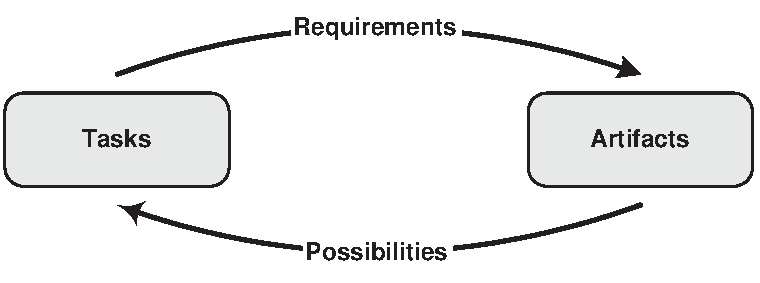
\includegraphics[height=4cm]
		{pictures/research_review/Ch2-TaskArtefactCycle.pdf}
	\end{center}
	\caption{The Task-artefact Cycle~\citep{Carroll-cycle:91}}
	\label{fig:TaskArtefactCycle}
\end{figure}
%% see~\citep{jc-cycle:91, jc-cycle:92}

%%%%%%%%%%%%%%%%%%%%%%%%%%%%%%%%%%%%%%%%%%%%%%%%%%%
%%%%%%%%%%%%%%%%%%%%%%%%%%%%%%%%%%%%%%%%%%%%%%%%%%
% \subsection{Technology and application domains within HCI}
%%%%%%%%%%%%%%%%%%%%%%%%%%%%%%%%%%%%%%%%%%%%%%%%%%
%%%%%%%%%%%%%%%%%%%%%%%%%%%%%%%%%%%%%%%%%%%%%%%%%%%
%% Firstly personal information management is identified as an important application domain within HCI.%%
%%  Huge Area. Need to focus within HCI: use of application domains?
%% Sutcliffe's taxonomy of interface technologies and application domains~\citep{sutcliffe:00}:
%% \textit{Applications} (CHECK) e.g. personal information management, design genres? (abstractions over artifacts)
% Interactive systems exist in many forms. 
\citet{Sutcliffe:00} sets out a framework which can be used to classify HCI knowledge in terms of the forms of interactive system to which that knowledge applies. Sutcliffe classifies interactive systems in terms of  \textit{architecture families} and \textit{application/functionality families}.
Architecture families represent different types of user interface components such as speech recognition and window management.
Application families represent the task domains to which interface components can be applied. Examples include finance and information retrieval.

% Specific architectural components can be applied to a range of application areas. For instance speech recognition functionality can be applied to financial or information retrieval interfaces.
\textbf{Section~\ref{bg:pim}} defined PIM in terms of four user activities, the \textit{acquisition} of items to form a collection of information, the \textit{organization} of those items, the \textit{maintenance} of the collection, and the subsequent \textit{retrieval} of items to satisfy the user's information needs.  Therefore, within Sutcliffe's framework, PIM is an application family, to which interface technology can be applied.








% \newpage
%%%%%%%%%%%%%%%%%%%%%%%%%%%%%%%%%%%%%%%%%%%%%%%%%%%%%%%%%%%%%%%%%%%%%%%
%%%%%%%%%%%%%%%%%%%%%%%%%%%%%%%%%%%%%%%%%%%%%%%%%%%%%%%%%%%%%%%%%%%%%%%
\subsection{Research on Personal Information Management}
\label{review:pim-research-overview}
%%%%%%%%%%%%%%%%%%%%%%%%%%%%%%%%%%%%%%%%%%%%%%%%%%%%%%%%%%%%%%%%%%%%%%%
%%%%%%%%%%%%%%%%%%%%%%%%%%%%%%%%%%%%%%%%%%%%%%%%%%%%%%%%%%%%%%%%%%%%%%%
%% \textit{THINK: Use of task-artifact cycle as a framework for describing the area and the theory-practice gap?}
% THINK: relate studies -> design -> theory (with T/A cycle?
%%%%%%%%%%%%%%%%%%%%%%%%%%%%%%%%%%%%%%%%%%%%%%%%%%%%%%%%%%%%%%%%%%%%%%%
% ALternate structure:
% Frame as intra-tool/cross-tool from the start
%In terms of improving support - three fundamental research/design approaches can be identified:
%1.	RESEARCH: model as separate PIM systems with own distinct issues, DESIGN: Improve the interface of specific tools (i.e. optimize separately)
%2.	RESEARCH: investigate how tools are inter-linked, DESIGN: Improve integration between PIM tools (i.e. optimize inter-working) - yet retain separation/specialization where it makes sense
%3.	RESEARCH: model as one PIM system encompassing multiple applications, DESIGN: Unify PIM support.
%Many examples of all three types. Do we focus on one type here in survey?
%%%%%%%%%%%%%%%%%%%%%%%%%%%%%%%%%%%%%%%%%%%%%%%%%%%%%%%%%%%%%%%%%%%%%%%
\citet{Whittaker-rta:00} note the importance of everyday computer-based activities such as PIM.  They highlight three criteria of task importance: (1) tasks that are carried out frequently, (2) tasks that are ``mission-critical'', and (3) real-world tasks that are rooted in studies of actual user practice.  The studies of PIM discussed in the next section show how 
PIM matches the first and third of these criteria, confirming the promise of research in this area.  Since PIM-tools are in continual use by many millions of users, even small improvements to tool design may have profound effects in terms of productivity savings and satisfaction improvements.
% They discuss how PIM matches the first and third of these criteria.  The promise of research in this area can be framed as follows.
% Therefore there is a high worth in improving interface support for them)
% Many studies have noted the fundamental nature of personal information management -- it is carried out by millions of computer users  many times a day.

%%%%%%%%%%%%%%%%%%%%%%%%%%%%%%%%%%%%%%%%%%%%
% WHY RESEARCH IS WORTHWHILE IN THIS AREA
%%%%%%%%%%%%%%%%%%%%%%%%%%%%%%%%%%%%%%%%%%%%
%% Effect of increased IT support on productivity~\citep{landauer:95,sellen:01}

%% Quick overview of the main types/areas/strands/threads of research to explain structure of literature review see \textbf{Figure ~\ref{fig:chapter2_substantive_summary}}:
In this chapter three main areas of research related to PIM are discussed.
%%: (1) empirical studies, and (2) prototype design. 
%%%%%%%%%%
% STUDIES
%%%%%%%%%%
\begin{itemize}

\item \textbf{Section~\ref{review:pim-empirical-review}} reviews \textit{empirical studies of PIM behaviour}. This body of work has been concerned with understanding the usage of existing PIM artefacts, observing users' needs and problems, and making recommendations for improving design.
%% Empirical studies (trying to understand the activity of PIM by analysing the usage of existing PIM artefacts, observing users' needs and problems, and making recommendations for improving design)
%%%%%%%%%%
% DESIGN
%%%%%%%%%%

\item  \textbf{Section~\ref{review:pim-technological-review}} reviews \textit{technological prototyping}, the second body of research.  The design of research prototypes (the design of new artefacts aimed at providing improved support for user needs). The contribution of technology design to HCI knowledge is also considered.
%% Designing research prototypes (the design of new artefacts aimed at providing improved support for user needs). The contribution of technology design to HCI knowledge is considered in terms of artefact theory

%%%%%%%%%%
% THEORY
%%%%%%%%%%
% \textbf{Section~\ref{review:pim-theory-review}} reviews relevant theory.
\item \textbf{Section~\ref{review:pim-theory-review}} then discusses \textit{theoretical work relevant to PIM}. The overall lack of theory in this area is highlighted. Relevant theory from related fields such as information retrieval is also identified.

\end{itemize}



%%%%%%%%%%%%%%%
% SIGNPOSTING
%%%%%%%%%%%%%%%
% In the next three sections each area of research is considered, including the main methods employed and key contributions  made.  


%%%%%%%%%%%%%%%%%%%%%%%%%%%%%%%%%%%
%%%%%%%%%%%%%%%%%%%%%%%%%%%%%%%%%%%
%%%%%%%%%%%%%%%%%%%%%%%%%%%%%%%%%%%
%%%%%%%%%%%%%%%%%%%%%%%%%%%%%%%%%%%


\newpage
%%%%%%%%%%%%%%%%%%%%%%%%%%%%%%%%%%%%%%%%%%%
%%%%%%%%%%%%%%%%%%%%%%%%%%%%%%%%%%%%%%%%%%%
\section{Review of Empirical Work}
\label{review:pim-empirical-review}
%%%%%%%%%%%%%%%%%%%%%%%%%%%%%%%%%%%%%%%%%%%
% Studies to add:
% Dix (HCI-International): when best to file?
%%%%%%%%%%%%%%%%%%%%%%%%%%%%%%%%%%%%%%%%%%%
%%%%%%%%%%%%%%%%%%%%%%%%%%%%%%%%%%%%%%%%%%%%%%%%%%%%%%%%%%%%%%%%%%%%%
% Wording:
% 	a number of studies have examined / provide evidence that
%%%%%%%%%%%%%%%%%%%%%%%%%%%%%%%%%%%%%%%%%%%%%%%%%%%%%%%%%%%%%%%%%%%%%
%%%%%%%%%%%%%%%%%%%%%%%%%%%%%%%%%%
% Where to place?
% QUESTION: do results hold across multiple tools?
%%%%%%%%%%%%%%%%%%%%%%%%%%%%%%%%%%
% Generic vs. Task-Specific~\citep{bn-slides:96}
%%%%%%%%%%%%%%%%%%%%%%%%%%%%%%%%%


%%%%%%%%%%%%%%%
% SIGNPOSTING
%%%%%%%%%%%%%%%
% \textbf{Section~\ref{review:pim-research-overview}} identified the main bodies of research that are concerned with personal information management.
%%%%%%%%%%%%%%%%%%%%%%%%%%%%%%%%%%%%%%%%%%%%%
%% 2 types: lab studies and field studies
%%%%%%%%%%%%%%%%%%%%%%%%%%%%%%%%%%%%%%%%%%%%%
%% Fieldwork: chance to view evolution of stratgies
%% Lab-studies: non-interactive pre-specified tasks, pre-specified tasks, easy-to-define objective metrics, efficiency bias
%% Relative predominance of fieldwork compared to lab studies.  Postulate reasons why in pros and cons.
%%
%% Also varying levels of abstraction across workspace -- PIM-related problems can be tackled at many different levels.
%% although still far from a systematic background of knowledge~\citep{Whittaker-rta:00}. 
% The aim of empirical work is to investigate a phenomena  with the intention of  providing increased understanding of that phenomena in the form of empirical data or theory development.
% The aim of such work is to examine how users employ current tools, identify the problems they encounter, and are useful in highlighting the aspects of current tool designs that are non-optimal. 
% Within HCI, empirical studies have constituted a large proportion of research into PIM.
This section reviews the first body of research related to PIM, \textit{empirical studies}. 
The aim of such work has been to investigate the use of current PIM-tools, and to improve understanding of user behaviour and needs. The output of such research thus provides requirements for the design of new PIM-tools.
%%%%%%%%%%%%%%%%%%
% FIELD STUDIES
%%%%%%%%%%%%%%%%%%
% The downside is that users select their own tasks to some extent, and it may hard to compare between users~\citep{newman:95}. % Whittaker \textit{et al}.~\citep{Whittaker-rta:00} note the need to employ both objective lab studies and field studies in the investigation of personal information management and evaluating tools.
Two types of empirical work can be identified: (1) field studies, and (2) controlled studies.
Field studies follow in the ethnomethodological research tradition of collecting data in real-world, naturalistic contexts. In contrast, controlled studies emphasise the collection of objective data in a lab context. They typically involve the user in carrying out a pre-specified task, thus enabling comparison across multiple participants, rather than necessarily reflecting real-world usage. 

%%%%%%%%%%%%%%%%%%%%%%%%%%%%%%%%%%%%%%%%%%%%%%
%% Aim of empirical work
%%%%%%%%%%%%%%%%%%%%%%%%%%%%%%%%%%%%%%%%%%%%%%%
%% should really cite this
%% \textit{THINK: What is the aim of such empirical findings -- motivate and direct design? What are their inherent limitations?}
%%
%% Aim: raise issues, build up rich picture of how users employ tools, problems they encounter, identify particular needs and scope for new design
The rest of this section is structured as follows.  Firstly, \textbf{Section~\ref{field-studies}} moves on to consider field studies of PIM in both the physical and digital domains. Then \textbf{Section~\ref{objective-studies}} considers objective studies of low-level cognitive phenomena associated with PIM. Finally, \textbf{Section~\ref{empirical-contribution-discussion}} discusses the overall contribution from research of this type.

%%%%%%%%%%%%%%%%%%%%%%%%%%%%%%%%%%%%%%%%%%%%%%%%%%%%%%%%%%
\subsection{Field Studies}
\label{field-studies}
%%%%%%%%%%%%%%%%%%%%%%%%%%%%%%%%%%%%%%%%%%%%%%%%%%%%%%%%%%
% think also include ContactMap study?
%% EXPAND THIS SECTION IN DETAIL? - is G and D a field study?
%%%%%%%%%%%%%%%%%%%%%%%%%%%%%%%%%%%%%%%%%%

% This section is divided into studies of PIM in the physical and digital domains.

%%%%%%%%%%%%%%%%%%%%%%%%%%%%%%%%%%%%%%%%%%%%%%
\subsubsection{Studies in the physical domain}
%%%%%%%%%%%%%%%%%%%%%%%%%%%%%%%%%%%%%%%%%%%%%%
%% EXPAND EXPAND EXPAND aka "`More detail to be included here."'
As noted in \textbf{Chapter~\ref{chapter:bg}}, physical metaphors such as the Desktop Metaphor and the folder hierarchy have greatly influenced the design of PIM-tools~\citep{smith:82}.  A number of researchers have studied information management practices in the physical domain with the aim of influencing the design of digital PIM-tools.

%%%%%%%%%%%
% MALONE
%%%%%%%%%%%
% information management in the real world has provided a strong influence on the design of PIM-tools.  In particular, a number of  including the  have the standard form of PIM-tools is based on the desktop metaphor representation of physical offices.
% soper:76,cole:82,
% An early and influential body of empirical studies focused on the management of documents in offices, e.g. ,kwas:91}.  
Tom Malone's work has been particularly influential in PIM research~\citep{tm:83}.  Malone highlighted the inherent difficulties that many users encounter in classifying and retrieving documents in the physical domain, and identified a number of routes which PIM-tools could follow to avoid such problems in the digital domains.  These included support for automatic classification.  Malone also observed the fundamental \textit{reminding} affordance of desks -- people do not only arrange documents to find them again, they also do so to remind themselves of things to do (i.e. to contextualize their work activity).  By doing so, Malone went beyond the traditional information management perspective that focuses on storing items for future retrieval.  Malone also identified two fundamental user strategies in managing paper documents: \textit{filing} and \textit{piling}.
%%%%%%%%%%%
% KWASNIK
%%%%%%%%%%%
%In her study of physical PIM, Kwasnik~\citep{kwas:91}
%identified a range of factors that influenced the
%classification included those based on attributes of the
%document content such as author and topic, and those based
%on document context such as importance and activity. A
%similar technique has been employed more recently in the
%electronic domain in studies of applied similar methods to
%the electronic domain, in their studies of
%files~\citep{barreau:95} and web bookmarks~\citep{gd:01}.
%In contrast to these previous studies, the analysis
%presented here is based on folder names (and the
%descriptions participants offered of those folder names
%offered during the guided tour), rather than on
%participants' descriptions of their classificatory
%behaviour.
% More detail to be included here.
\citet{kwas:91} reports an investigation of classification practices in a physical office. Her study identified a number of contextual factors that influence classification decisions.  She concluded that people do not make classificatory decisions based purely on document attributes, e.g. title and author.  More recently, similar studies have been performed of the classification of files~\citep{barreau:95} and web bookmarks~\citep{gd:01}.
% Both of these studies have had a substantial influence on many later studies in the digital domain.

%%%%%%%%%%%%%%%%%
% More recent
%%%%%%%%%%%%%%%%
There have also been a number of contemporary studies in this area.  \citet{Whittaker-paper:01} took advantage of an office relocation to observe physical information management strategies. They present three main findings. Firstly, they observed that many people are irrational in terms of the information they manage, for instance they keep many items available elsewhere.  Secondly, they noted that many people employ a mixture of the piling and filing strategies identified by~\citet{tm:83}, and observed that filers tended to amass more information than pilers.  They also noted the importance of older archived information for many people, adding to the debate in this area (see next section). % ~\citep{bn:95,kidd:94,Gelernter:96a}.
%% define filers and pilers
\citet{sellen:01} note the large amount of time wasted by office managers in managing information, leading to a distraction from their primary job roles.  They suggest that there is a significant impact on manager productivity from PIM in the physical and digital domains.
%  More detail to be included here.
%% EXPAND EXPAND EXPAND aka "`More detail to be included here."'


%%%%%%%%%%%%%%%%%%%%%%%%%%%%%%%%%%%%%%%%%%%%%%%%%%%%%%%%%%
\subsubsection{Studies in the digital domain}
\label{digital-studies}
%%%%%%%%%%%%%%%%%%%%%%%%%%%%%%%%%%%%%%%%%%%%%%%%%%%%%%%%%%

Most studies in the digital domain have focused on user behaviour within specific PIM-tools.  This section highlights a number of key findings of relevance to the work in later chapters.  \textbf{Table~\ref{table:empirical_studies_summary}} offers a summary of the studies that have been performed.
%% More recent studies in the digital domain have focused on the various applications that support PIM.
The main focus to date has been on \textit{email}, e.g.~\citep{Whittaker-email:96,Ducheneaut:01}, \textit{web bookmarks}, e.g.~\citep{da:98,gd:01,kftf:01} and \textit{files}, e.g.~\citep{barreau:95,bn:95}.  In addition, many other types of personal information have been studied including \textit{photos}~\citep{kr:03}, \textit{time and task management}~\citep{sp:93,bg:01,palen:98}, \textit{contacts}~\citep{Whittaker-contacts:02}, \textit{instant messaging}~\citep{Whittaker-im:02}, and \textit{voicemail}~\citep{Whittaker-jotmail:00}.  Since the first three -- files, email and bookmarks -- act as the main focus of the empirical and design work in \textbf{Chapters~\ref{chapter:exploratory_study}} to \textbf{\ref{chapter:main-study}} of this thesis, they are also the focus of this review.  
%% 
% In general there is too much to survey, but some findings can be extracted that have relevance across multiple technological formats.


%%%%%%%%%%%%%%%%%%%%%%%%%%%%%%%%%%%%%%%%%%%%%%%%%%%%%%%
% TABLE: SUMMARY OF EMPIRICAL STUDIES
% Table generated by Excel2LaTeX from sheet 'Sheet1'
% in tables/ch2/ch2-tables.xls
%%%%%%%%%%%%%%%%%%%%%%%%%%%%%%%%%%%%%%%%%%%%%%%%%%%%%%%
\begin{small}
\begin{table}[hbtp]
\begin{center}
\begin{footnotesize}
\setlength{\extrarowheight}{2pt}
\begin{tabular}{|p{4cm}|p{7cm}|}
\hline
{\bf Type of information} & {\bf Studies} \\
\hline
Physical documents & \citep{tm:83,kwas:91} \\
\hline
Files (including the file system and desktop icons) & \citep{jc:82,akin:87,barreau:95,bn:95,Kaptelinin:96} \\
\hline
     Email & \citep{wm:88,Whittaker-email:96,ob:97,Ducheneaut:01} \\
\hline
Web bookmarks & \citep{da:98,gd:01,kftf:01,dix:03a} \\
\hline
    Images & \citep{kr:03} \\
\hline
 Voicemail & \citep{Whittaker-jotmail:00} \\
\hline
  Contacts & \citep{Whittaker-contacts:02} \\
\hline
Calendar and to-do items & \citep{sp:93,bg:01,palen:98} \\
\hline
Instant messaging & \citep{Whittaker-im:02} \\
\hline
\end{tabular}  

\end{footnotesize}
\caption{Summary of empirical studies of different PIM-tools}
\label{table:empirical_studies_summary}
\end{center}
\end{table}
\end{small}

%%%%%%%%%%%%%%%%%%%
% EMAIL DISCUSSION
%%%%%%%%%%%%%%%%%%%
% Email: generally most popular - although many studies focus on its usage as a collaborative tool. Whittaker~\citep{Whittaker-email:96}, Balter~\citep{ob:97,ob:00}, Duchaneaut~\citep{Ducheneaut:01}, Mackay~\citep{wm:88}. Also CSCW2002 workshop.
%%%%%%%%%%%%%%%%%%%
% WEB BOOKMARKS
%%%%%%%%%%%%%%%%%%%
% Web bookmarks: Abrams~\citep{da:97,da:98}, KFTF~\citep{kftf:01}, G\&D~\citep{gd:01}, Dix~\citep{dix:03a}

%%%%%%%%%%%%%%%%%%%%%%%%%%%%
% BARREAU
%%%%%%%%%%%%%%%%%%%%%%%%%%%%
Based on her study of file management, Barreau presents a conceptual framework that conveys the complex, high-level nature of PIM~\citep{barreau:95}.  In summary, she identified five aspects of the functionality provided by PIM-systems: (1) \textit{acquisition} of items into a collection, (2) \textit{organization} of items, (3) \textit{maintenance} of the collection (e.g. archiving items into long-term storage), (4) \textit{retrieval} of items for reuse, and (5) \textit{output} of the information in an appropriate format  This framework is discussed in more detail in \textbf{Section~\ref{bg:pim}}.  Barreau highlights the idiosyncratic nature of PIM leading to a wide variety of strategies between individuals, and the consequent need for tool flexibility. Barreau also notes the \textit{satisficing} nature of PIM: the people in her study only tended to acquire information as it was required, and only maintained their information when they were forced to by circumstances such as running out of space.
% More detail to be included here.

%%%%%%%%%%%%%%%%%%%%%%%%%%%%
% PROBLEMS
%%%%%%%%%%%%%%%%%%%%%%%%%%%%
%% MOVE TO LIMITS OF HIERARCHY STUDY? limits of hierarchy
Many studies have highlighted the problems users encounter in PIM sub-activities such as organization and retrieval.   % Many studies have concluded by calling for improved ``intelligent'' support for classification but it is not clear whether this would benefit users. Indeed many users choose not to use personal classification schemes, and instead rely on implicit metadata and search mechanisms for finding information . When users do file, they typically exhibit satisficing behaviour and ``just do enough to get by~\cite{barreau:95}.  This leads to problems such as premature filing and failed folders.
% Many of the studies of real-world PIM have noted the large amount of effort that users often devote to filing information (e.g. Bellotti and Smith 2000). Several researchers identify a trade-off between the time investment of up-front organization, versus the costs of not being able to find items in subsequent retrieval (B�lter 2000, Whittaker and Hirschberg 2001).
Lansdale highlights the core psychological difficulties inherent in the low-level processes of organization and retrieval~\citep{ml:88}.  He observes that classification is a cognitively difficult task with users having to deal with problems of ambiguous and overlapping categories. Users often employ a satisficing strategy, resulting in problems such as misfiling, failed folders, and filing prematurely before the value of an item has been assessed~\citep{Whittaker-email:96}.  Alternatively, users may not file, and rely on retrieving information via sorting based on implicit metadata, and search.  Such loose classification facilitates additional retrieval cues such as location, time and appearance. However, such strategies are rarely scalable (ibid).  Lansdale identifies two psychological processes that are used when retrieving information: (1) \textit{recall-directed search} (to home in on a group of items), and (2) \textit{recognition-based scanning} (selecting a particular item). He notes that retrieval systems are not tuned to the abilities of the human memory, such as  the ability to remember general meanings better than specific details. Users are forced to remember specific filenames and locations, whilst human memory is better at handling contextual information such as time and colour.
% The following technological criticisms have also been levelled against the
% folder hierarchy. 

%%%%%%%%%%%%%%%%%%%%%%%%%%%%%%%%%%%
% Types of personal information
%%%%%%%%%%%%%%%%%%%%%%%%%%%%%%%%%%%
%Several other researchers have proposed a similar break-down.
%%%%%%%%%%%%%%
% Also Soper, Malone?
%%%%%%%%%%%%%%
Several studies have surveyed the types of information that are managed by users.
\citet{bn:95} identify three types of information in terms of their lifetime of use: \textit{ephemeral}, \textit{working}, and \textit{archived}.  Ephemeral information is valued in the short-term and includes to-do items and information for immediate use.  Working information is valued over a longer period and may be kept for the period of a particular project over several months.  Archived information is kept in the long-term but is not in day-to-day use. There has been some disagreement over which is the most important type of information to focus on with design work. \citet{bn:95} highlight the relative importance of ephemeral/working information (accessed via location-based finding) over archived material (and the use of search).  This view is echoed by \citet{kidd:94} who argues that too much design is focused on supporting the management of older archived information.  In contrast, other researchers have argued the importance of archived information~\citep{Gelernter:96b,Whittaker-paper:01}.

%%%%%%%%%%%%%%%%%%%%%%%%%%%%%%%%
% \subsubsection{PIM strategies}
%%%%%%%%%%%%%%%%%%%%%%%%%%%%%%%%

Influenced by Malone's work, several studies have attempted to classify management strategies in various PIM-tools, with a particular focus on how users organize items. \citet{Whittaker-email:96} observed 3 types of strategies for managing email: \textit{frequent filer}, \textit{spring cleaner} and \textit{no-filer}. \citet{ob:97} extends this classification by dividing the no-filer class into two further sub-classes: \textit{folderless cleaner} and \textit{folderless spring-cleaner} (depending on whether old items are deleted from the inbox on a daily basis). \citet{da:98} proposed a similar classification of bookmark management strategies: \textit{no-filer}, \textit{creation-time filer}, \textit{end-of-session filer}, and \textit{sporadic filer}. The author is not aware of any strategy classifications in files.
% Within Barreau's model these classifications correspond to the organizing sub-activity, but as many of the above researchers note, they have a strong influence on the type of retrieval strategies employed.
%% Although note link from org/maint to retrieval strategies (more folders -- more browsing)

%%%%%%%%%%%%%%%%%%%%%%%%%%
% BROWSE VERSUS SEARCH
%%%%%%%%%%%%%%%%%%%%%%%%%%
In terms of retrieval, \citet{bn:95} identify a strong preference for location-based finding over the use of search.  They define location-based finding as the browsing of information via the organizational structure developed by the user. Their results have been strongly criticised by \citet{Gelernter:96a} who note that infrequent use of search can be explained by the poor design of search functionality in most operating systems. \citet{Gelernter:96a} call for further study of the use of advanced search technology.  However, it can be observed that later studies, including the one reported in \textbf{Chapter~\ref{chapter:exploratory_study}}, reinforce Barreau and Nardi's observation of a preference for browsing over search\footnote{The \textit{Stuff I've Seen} system~\citep{Dumais:03a} offers a unified search interface across a range of PIM-tools. Dumais \textit{et al}'s evaluation results suggest that the improved search technology in their prototype lead participants to depend less on filing and browsing-based retrieval.}.


%%%%%%%%%%%%%%%%%%%%%%%%%%%%%%%%%%%%%%
% Cross-tool/issues of integration
%%%%%%%%%%%%%%%%%%%%%%%%%%%%%%%%%%%%%%
% although the empirical body of work has made many pertinent observations and recommendations, a key limitation can be observed findings have been fragmented along tool/application boundaries. Little guidance is provided for the developers of integration/unification technologies.
%% segmentation of research
%% Application-centricity of requirements (piecemeal) -- knock-on influence on later stages of design (and choice of embedding, unifying design strategies)
% However there has been little consideration of PIM as a cross-tool phenomenon (one that involves the use of multiple tools).  Do individuals employ similar strategies in email as they do in files? How are these tools used together? These questions need to be addressed to provide an empirical foundation for the many systems proposed to improve integration between PIM tools (see below).
%%%%%%%%%%%%%%%%%%%%%%%%%%%%%%%%%%%%%%%%%%%%%%%%%%%%%%%%%%%%%%%%%%%%%%%%%%%%
%% But rare. Later than mine~\citep{goncalves:03a}
% One of the few other observations is by~\citep{bn:98} who observe users in need for better data transfer/handling of structured information.
%%  CHECK, should this be moved up into the strategy section above???
% \textit{A range of studies have focused on the sub-activities that make up PIM. \citet{jc:82} carried out a detailed study of the strategies used to name files in an early version of DOS. A number of studies have focused on the organization sub-activity of PIM~\citep{kwas:91,barreau:95,gd:01}.}
% Self-focused field studies in which researchers everything have also been carried out ~\citep{bell:01,pwilson:01,dix:02}. Provide vision of the ultimate PIM-tool, but it is not clear whether these prophecies reflect actual user needs or just the researchers' ambitions.
%% darpa-lifelog:03}
%% Total Recall http://bourbon.usc.edu/iml/recall/
%%%%%%%%%%%%%%%%%%%%%%%%%%%%%%%%%%%%%%%%%%%%%%%%%%%%%%%%%%%%%%%%%%%%%%%%%%%%
The prime focus of this thesis is on improving \textit{integration} between PIM-tools. 
However, few studies have investigated user behaviour beyond a tool-specific context.  Exceptions are discussed as follows. \citet{Kaptelinin:96,Kaptelinin:03} observes that users often employ multiple PIM tools in support of their high-level activities, such as the Desktop, the file system, and email.  He notes the difficulties users encounter in performing key project tasks across tool boundaries, such as archiving.   He also observes the duplication of organizational schemes between digital and physical documents.
\citet{Bellotti:00} similarly note how the management of information related to a particular activity is distributed across a wide range of tools.  Furthermore, they note that information of a particular technological format is often compartmentalized between different PIM-tools, e.g. files or reminders.  Like Kaptelinin, Bellotti and Smith observe the duplication of filing systems between different PIM-tools. However, neither study reports a detailed investigation of the extent of such duplication.  Two other studies have noted how users perform task and time management across a wide range of PIM-tools and physical artefacts~\citep{bg:01,Bellotti:03}.  Similarly, \citet{kftf:01} note how users manage web references with a wide range of mechanisms including bookmarks, email, ad-hoc lists, and physical print-outs.  All these studies make calls for improved integration between different tools. 



%%%%%%%%%%%%%%%%%%%%%%%%%%%%%%%%%
\subsection{Controlled Studies}
\label{objective-studies}
%%%%%%%%%%%%%%%%%%%%%%%%%%%%%%%%%

% \textit{They have been used primarily with this area to investigate low-level aspects of PIM.}

%% ADD: Hierarchy stuff (e.g. Williges stuff)
%  Use of 3D -- Robertson, Cockburn. \textit{Move to evaluations?}
% The previous section discussed field studies of personal information management. Here lab studies are considered. Note that study-based evaluations of PIM-tools are discussed in \textbf{Section~\ref{review:pim-technological-review}}.
% % Since they are not directly relevant to the scope of the thesis, a brief summary is provided as follows.
As well as field studies of naturalistic PIM behaviour, a number of controlled studies have also been carried out in the area.  Since the research reported in this thesis employs a field-study methodology, only a brief overview of two controlled studies is provided.  A number of controlled studies have also been carried out to evaluate new PIM designs (see \textbf{Section~\ref{review:pim-technological-review}}).

%%%%%%%%%%%%%%%%%%%
% DUMAIS AND JONES
%%%%%%%%%%%%%%%%%%%
% A number of studies have focused on how users classify information. 
%$ report a comparison of spatial versus symbolic means of storage and retrieval. ADD.
\citet{Dumais:85} carried out a paper-based experiment designed to test the frequent assumption that spatial memory is more effective than symbolic memory.  Participants were asked to organize a series of items, using a combination of location-based (spatial) and name-based (symbolic) filing systems.  Over a series of retrieval tasks, spatial filing was seen to offer no benefit over symbolic filing.  Furthermore, retrieval speeds for location-only deteriorated significantly as more items were added.  Based on their findings, Dumais and Jones suggest that spatial management should not replace symbolic techniques, but instead act as an adjunct, much as in current desktop computers.

% \citet{ml:88} report comparisons of user performance in recall versus recognition tasks. ADD.
% how the time at which bookmarks are filed affects retrieval performance.  ADD.
\citet{dix:03a} report an investigation of how retrieval performance depends on the time at which bookmarks are organized.  Two conditions were compared: ``sorting during browsing'', and ``sorting after browsing''.  Based on performance in a series of questions that involved retrieval from the set of bookmarks, the ``sorting after browsing'' resulted in significantly faster recall.  However, the difference was not evident when users were tested a week later.  Dix and Marshall suggest that the initial result may be due to the close proximity of the sorting and post-test tasks.  

A key criticism that can be levelled at such controlled studies is that they lack ecological validity. Although a number of interesting results are presented, the relevance of the findings to real-world contexts can be questioned.  Dix and Marshall themselves highlight two limitations of the ecological validity of their experiments: (1) the bookmarks were pre-selected, and (2) in real-life users may use a combination of during and after-browsing sorting.  \citet{Whittaker-rta:00} call for the employment of both field and controlled studies in PIM research.


%%%%%%%%%%%%%%%%%%%%%%%%%%%%%%%%%%%%%%%%%%%%%%%%%%%%%%%%%%%%%%%%
\subsection{Discussion of Empirical Contributions}
\label{empirical-contribution-discussion}
%%%%%%%%%%%%%%%%%%%%%%%%%%%%%%%%%%%%%%%%%%%%%%%%%%%%%%%%%%%%%%%%
% The section has so far reported the main findings from empirical studies directed at understanding the activity of PIM by analysing the usage of existing PIM artefacts, observing users' needs and problems, and making recommendations for improving design. Here the contribution offered by empirical studies is discussed and recommendations are expressed regarding the direction of future empirical research.

%%%%%%%%%%%%%%%%%%%%%%%%%%%%%%%
% 1. OVERALL: UNDER-RESEARCHED
%%%%%%%%%%%%%%%%%%%%%%%%%%%%%%%
%% %The general limitations of studies thaht have been carried out include questions over their statistical significance. e.g. closed user groups Knowledge Workers~\citep{kidd:94}
%% We now  We need more powerful PIM interfaces. Research from 1995 *should* be ignored. Discuss (-;
%% THINK about use of empirical findings?
% Generally studies have been aimed at providing increased understanding, make design recommendations, offer requirements for design, build theory.
% In terms of future research, in general more empirical groundwork is required in terms of the conceptual groundwork required for research in this area such as defining a descriptive vocabulary~\citep{Whittaker-rta:00}.
Although many interesting findings have been presented, the author echoes the view of~\citet{Whittaker-rta:00}, that there is still a lack of systematic empirical investigation in this area.  They propose a simple criterion for this: \textit{are there at least two user studies in a given area?}  Although this can be considered to be a highly conservative requirement given the ubiquity and importance of PIM, they note that even this criterion is not met. They conclude that there is no accepted body of knowledge to build further research on, for example a consensus of people's tasks and problems, and appropriate metrics for evaluation. % The lack of understanding can also be illustrated by the general disagreement over key issues such as the importance of PIM-tool support for different types of information. % In summary, the field is in an immature state.  Another limitation identified by the author is that technology has moved on from some of the se
% Although one or two studies have explored the usage of most tools in common use, Whittaker \textit{et al}. note that there is still a core lack of understanding. 
% A key cause of this situation is the complexity and range of phenomena associated with PIM. 
Three further limitations are identified by the author as follows.

%%%%%%%%%%%%%%%%%%%
% 2 INTEGRATION
%%%%%%%%%%%%%%%%%%%
The expressed focus of this thesis is on PIM-integration, and as the next section discusses there has been much design interest in this area. % It has been shown that a user will often employ multiple PIM tools in support of their high-level activities~\citep{Kaptelinin:96}. 
% there has been little consideration of PIM as a cross-tool activity (one that involves the use of multiple tools). 
However, the majority of studies have been tool-specific and are concerned with the management of information of a particular technological format (e.g. files, email, bookmarks). In terms of the wider personal information environment this represents an inherently piecemeal approach. \textbf{Section~\ref{review:discussion}} discusses this limitation in more detail.

%%%%%%%%%%%%
% 3 LONGIT
%%%%%%%%%%%%
%% A second limitation is the lack of attention to how PIM strategies may change over time. 
Another issue that illustrates the need for more studies in this area is the lack of empirical  attention paid to longitudinal aspects of PIM, e.g. how PIM strategies may change over time~\citep{ml:92}.  Instead, most work to date has been based on short-term ``snapshots'' of user behaviour % Exceptions are discussed~\citep{ob:97}. More understanding of longitudinal issues relating to PIM is required. Do PIM strategies change over time, and if so how?


%%%%%%%%%%%%%%%%%%%%%%%
% 4. WRONG TYPE OF USER
%%%%%%%%%%%%%%%%%%%%%%%
Finally, it is observed that most studies have focused on small groups of technical users.  It can be argued that such samples are unrepresentative of the wider population of users, including non-technical ``home'' users.
%% can I think of any counter-examples?
% It is noted that many of these users in early studies did not have hard disks, let alone email.  
% Users are much much more sophisticated today and have lots more info in lots more forms.  
Furthermore, many of the most often cited studies were carried out almost a decade ago, e.g.~\citep{bn:95}. For example, Barreau~\citep{barreau:95} mentions a few users who stored information on floppies as they did not have hard drives. Although some results will be transferable to modern personal information environments, it is envisaged that user needs may have moved on from 1995. % In other words further investigation is required. At the very least research should be extended to cover other types of user. The lack of work directed at  is highly evident.


%%%%%%%%%%%%%%
% TRANSFER
%%%%%%%%%%%%%%
% Finally it is noted that empirical findings have not been effectively used by other areas of research. For example little theory has been built on empirical data~\citep{ob:97,ob:00}, and there are few examples of how empirical data has been effectively leveraged in design~\citep{Bellotti:00,Whittaker-contactmap:02b}. Overall there is a lack of systematic understanding of users activities, problems, and needs to guide design work.


%%%%%%%%%%%%%%%%%%%%%%%%%%%%%%%%%%%%%
% \subsubsection{Directions for future empirical research}
%%%%%%%%%%%%%%%%%%%%%%%%%%%%%%%%%%%%%%

%%%%%%%%%%%%%%%
% SIGNPOSTING
%%%%%%%%%%%%%%%
%This section reviewed the first research area identified in \textbf{Section~\ref{review:pim-research-overview}}: empirical studies of PIM.
The next section discusses the second area of research contributions: the design and prototyping of new PIM-tool software.

%%%%%%%%%%%%%%%%%%%%%%%%%%%%%%%%%%%
%%%%%%%%%%%%%%%%%%%%%%%%%%%%%%%%%%%
%%%%%%%%%%%%%%%%%%%%%%%%%%%%%%%%%%%
%%%%%%%%%%%%%%%%%%%%%%%%%%%%%%%%%%%

\newpage
%%%%%%%%%%%%%%%%%%%%%%%%%%%%%%%%%%
%%%%%%%%%%%%%%%%%%%%%%%%%%%%%%%%%%
\section{Review of Technological Prototypes}
\label{review:pim-technological-review}
%%%%%%%%%%%%%%%%%%%%%%%%%%%%%%%%%%
% Possible alternative structures for this section.
% A) Divide as intra-tool, integrating, cross-tool.
% B) Use \textbf{Chapter 2} conceptual framework to structure design work
%		 (in terms of aspects of PIM, or technological formats).
% C) Divide as commercial, research-oriented
%%%%%%%%%%%%%%%%%%%%%%%%%%%%%%%%%%
%%%%%%%%%%%%%%%%%
% WHERE TO PLACE:
%%%%%%%%%%%%%%%%%
% \begin{itemize}
%	\item \textit{PIM Managers~\citep{kaplan:90}}
% \end{itemize}

%%%%%%%%%%%%%%%
% SIGNPOSTING
%%%%%%%%%%%%%%%
% \textbf{Section~\ref{review:pim-research-overview}} identified three main areas of research that have been concerned with personal information management.
% For the purposes of this literature review they are bundled with research-derived design.  
% current tools in the public domain and surveyed in .
%% Provide sign posting to traditional tool analysis/survey earlier in \textbf{Chapter~\ref{chapter:bg}} for survey of current commercial tools (see above).
\textbf{Section~\ref{bg:pim-tools}} surveyed PIM-tools in common use.  This section reviews exploratory PIM prototypes that have been proposed in the research domain, as well as highly innovative commercial systems that are not in widespread use.
%%%%%%%%%%%
% CAVEAT
%%%%%%%%%%%
% Since a wide range of work falls under this category, and the main concern in this thesis is to survey work aimed at providing integration between PIM-tools, only a representative summary is provided. A focus is taken on systems which have provided improved support for organization.
%% Both in research and commercial sectors.
This is an active area of design, and many systems have been proposed, particularly in the commercial sector. Therefore, this section does not aim to be an exhaustive summary, but to instead provide a representative summary.

%%%%%%%%%%%%%
% STRUCTURE
%%%%%%%%%%%%%
% A focus is taken on systems that aim to improve integration between PIM-tools.Three main design genres can be identified in terms of : (1) intra-tool design, (2) inter-tool integration, and (3) unification.
The section is structured in terms of four design genres, defined in terms of the \textit{level of integration} they provide:

\begin{itemize}

%%%%%%%%%%%%%%%%%%%%%%%%
% Tool-specific design
%%%%%%%%%%%%%%%%%%%%%%%%
%% Refer to web survey online?
%% \textit{THINK: Inherently out-of-date after publication!}
% The first genre is design aimed at improving support for the management of a particular type of information within an existing PIM tool - i.e. the optimization of independent PIM systems -- integration is not a main design aim. See  for an overview , but note this is not the main focus of the thesis.
\item \textit{Tool-specific design} -- \textbf{Section~\ref{review:intra-tool}} provides an overview of new technology aimed to improve the design of specific PIM-tools such as email.  Integration is not a primary design aim of such work.

%%%%%%%%%%%%%%%%%%%%%%%%
% Integration increase
%%%%%%%%%%%%%%%%%%%%%%%%
 % The second design genre is aimed at  -  See 
%% (e.g. Apple Data Detectors, the Context toolkit)
\item \textit{Systems that provide increased integration between distinct PIM-tools} -- \textbf{Section~\ref{review:integration}} surveys this second genre, aimed at improving integration between distinct PIM tools. %, i.e. retaining distinct PIM systems but providing  bridge between them.

%%%%%%%%%%
% EMBEDDING
%%%%%%%%%%
\item \textit{Designs that embed additional support for the management of multiple types of information within one PIM-tool} -- \textbf{Section~\ref{review:embedding}} covers the embedding design genre. % , which has focused on 

%%%%%%%%%%
% UNIFYING
%%%%%%%%%%
\item \textit{Unifying designs that consolidate the management of multiple types of information within a single interface} -- \textbf{Section~\ref{review:unifying}} covers this final genre which represents the most ambitious design work in this area.  % Within this genre two sub-genres can be identified: (1) \textit{embedding} designs, and (2) \textit{unifying} designs. 

\end{itemize}

% %%%%%%%%%%%%%%%%%%%%%%%%%%%%%%%%%
% FIGURE - PIM-tool design space
%%%%%%%%%%%%%%%%%%%%%%%%%%%%%%%%%%%
% \begin{figure}
%	\begin{center}
%		\leavevmode
%		
\includegraphics[height=2in, width=.9 \textwidth]{pictures/research_review/Ch2-TechDesignSpace.pdf}
%	\end{center}
%	\caption{PIM-tool design space}
%	\label{fig:review:tech_design_space}
%\end{figure}


%%%%%%%%%%%%%%%%%%%%%%%%%%%%%%%%%%%%%%%%%%%%%%%%%%%%%%%%%%%
\subsection{Intra-tool Designs}
\label{review:intra-tool}
%% expand on piles
%%%%%%%%%%%%%%%%%%%%%%%%%%%%%%%%%%%%%%%%%%%%%%%%%%%%%%%%%%%

This section considers design work within \textit{tool-specific} contexts.  Since the focus of the thesis is on the provision of improved integration between PIM-tools, only a representative sample of tool-specific work is provided.
% aimed at improving support for the management of specific types of information. This design genre is not concerned with improving integration between different technological formats. Instead the work described here is aimed at optimizing distinct PIM systems dedicated to managing information in a particular technological format.  Three areas of design are discussed.
% The main concern of this thesis is providing integration between PIM-tools, only a representative summary is provided. A focus is taken on systems which have provided improved support for organization.
%% Both in research and commercial sectors.


%%%%%%%%%%%%%%%%%%%%%%%
% automatic filing
%%%%%%%%%%%%%%%%%%%%%%%
% However, questions remain after their evaluation, notably the potential loss of control by the user.  In addition, 
%% EXPAND EVALUATION
Many studies have observed the problems encountered by users in classifying items, e.g.~\citep{tm:83,Whittaker-email:96}.  Several prototypes have offered automatic filing of email messages based on user modelling techniques, e.g. the \textit{Mailcat} system~\citep{mailcat:99}.  The system automatically processes incoming mail through an adaptive classifier, and suggests the three most likely folders for the message to be filed in.  A long-term study in the context of the authors' own email usage revealed an accuracy rate of 85\%.  Although later systems have improved performance, such systems require some level of user monitoring which may be problematic.  Furthermore, \citet{Shneiderman:97} observe that such intelligent interfaces may result in a loss of control on the part of the user.


%%%%%%%%%%%%%%%%%%%%%%%%%%%%%
% multiple classification
%%%%%%%%%%%%%%%%%%%%%%%%%%%%%
% Aim here to deal with limitations of file+folder paradigm within the context of a specific type of information. 
% \textit{Haystack} system is set apart by the fact that a published evaluation has been performed. The evaluation was performed within the context of a controlled study.  Although the system was received positively, no objective improvements in retrieval time were observed. The need for a follow-up long-term evaluation is highlighted in the context of users's natural behaviour and information. %  Furthermore, the evaluation task was not a natural example of bookmark management which happens incrementally over time for many users~\citep{da:98}. 
Other prototypes have focused on a key limitation of the folder hierarchy, that of multiple classification not being supported, e.g.~\citep{haystack:03b}. Several commercial tools also provide multiple-classification support including \textit{BookKey} and \textit{GMail}.    Such systems allow a user to assign arbitrary user-defined attributes to an item, and then to retrieve them using any combination of those attributes.  Quan \textit{et al} report an evaluation of a multiple classification interface for managing bookmarks based on a flat set of attributes.  Users welcomed the multiple classification functionality, and there was some improvement in retrieval speed. However, the experiment can be criticized in terms of ecological validity, as a pre-selected data set was employed.  Furthermore, several limitations were observed including: (1) duplicated attributes, and (2) poor support for data that is naturally hierarchical.  The author urges further evaluation in a real-world setting.


%%%%%%%%%%%%%
% PILES
%%%%%%%%%%%%%
% At the small scale: piles~\citep{piles:92}. More detail to be included here.
%% think should piles be in spatial area?
%% EXPAND EXPAND EXPAND aka "`More detail to be included here."'


%%%%%%%%%%%%%%%%%%%%%%%%
% visualization schemes
%%%%%%%%%%%%%%%%%%%%%%%%%
% allowing the user to perform  by leaving items in piles
% A number of other prototypes have provided improved support for the visualization of hierarchical information (e.g. treemap, polyarchy work at Microsoft).
% On the desktop, the Piles system replicates piles of documents observed in the physical context~\citep{tm:83} in a digital context, and thus facilitates 
Other tool-specific work has offered new interactive techniques for representing collections of items.  The \textit{Piles} system~\citep{piles:92} allows the ``casual organization'' of items, a digital equivalent to the piling strategies observed by Malone in physical office environments~\citep{tm:83}. 
%%%%%%%%%%%%%%%%%%%%%%%%%%%%%%%%%%%%%%%%%%%%%%%%%%%%%%%
% \subsubsection{Spatial approaches to unification}
%%%%%%%%%%%%%%%%%%%%%%%%%%%%%%%%%%%%%%%%%%%%%%%%%%%%%%%
% RECONSIDER: is spatial really means of unification?
%%%%%%%%%%%%%%%%%%%%%%%%%%%%%%%%%%%%%%%%%%%%%%%%%%%%%%%
% A number of systems have been proposed that allow multiple types of personal information to be managed spatially. Three main types can be identified. The first type are spatial systems such as ROOMS~\citep{rooms:86} and Task Gallery~\citep{gr:00} which are more an integrative framework within which applications can exist. These can be considered alternatives or extensions of the desktop metaphor.
% More detail to be included here.
% Also consider Info Viz~\citep{card:91,card:96}
%% EXPAND EXPAND EXPAND aka "`More detail to be included here."'
% Second, there systems that provide spatial 
% More detail to be included here.
%% EXPAND EXPAND EXPAND aka "`More detail to be included here."'
%The final type are spatial hypertext systems~\citep{shipman:01}.
% More detail to be included here.
% Question: has this been evaluated? Is PIM a main design aim of this?
%% EXPAND EXPAND EXPAND aka "`More detail to be included here."'
Other prototyping has offered 3D spatial environments for managing information such as bookmarks, e.g. \textit{Data Mountain}~\citep{gr:98}.  However, the benefits of such a 3D approach have been questioned in follow-up work~\citep{ac:01}. Although users preferred the 3D interface, Cockburn and McKenzie observed slower retrieval times compared to a 2D system.

%% or email stuff from Lotus. TIDY

%%%%%%%%%%%%%%%%%%%%%%%%%%%%%%%%%%%%%%%%%%%%%%%%%%%%%%%%%%%%%%%%%%%%%%
% Other examples of intra-tool design that can be left out for now
%%%%%%%%%%%%%%%%%%%%%%%%%%%%%%%%%%%%%%%%%%%%%%%%%%%%%%%%%%%%%%%%%%%%%%
%Other prototypes have been poroposed to provide mproved support for specific technological formats including images~\citep{kuch:99,kr:03}, bookmarks (Saul stuff, Hunter-Gatherer, YelloPen) and voicemail~\citep{Whittaker-jotmail:00,Whittaker-scanmail:02}.

%%%%%%%%%%%%%%%%%%%%%%%%%
%%%%%%%%%%%%%%%%%%%%%%%%%
%%%%%%%%%%%%%%%%%%%%%%%%%
%%%%%%%%%%%%%%%%%%%%%%%%%


%%%%%%%%%%%%%%%%%%%%%%%%%%%%%%%%%%%%%%%%%%%%%%%%%%%%%%
\subsection{Improving Integration between Distinct PIM-tools}
\label{review:integration}
%%%%%%%%%%%%%%%%%%%%%%%%%%%%%%%%%%%%%%%%%%%%%%%%%%%%%%
% In this section designs are described which retain the separation between tools that manage different types of information, but attempt to improve integration between them. % Systems which go the whole way are discussed in the next section. 
%%
% Note that 
%% \textit{THINK: (OVERLAP ABOVE with current technology). 
%% Many areas, consider using a ``workspace diagram'' to frame all the different integration-related problems}
% A number of research systems have provided new forms of integration between current, distinct PIM-tools. 



%%%%%%%%%%%%%%%%%%%%%%%%%%%%
% STRUCTURED INFORMATION
%%%%%%%%%%%%%%%%%%%%%%%%%%%%
% Structured information, such as web addresses and email addresses appears in a wide range of personal information. Such structured information follows a standard format and can be easily identified by straight-forward pattern matching software.
% Current PIM-tools provide integration with other PIM-tools by allowing the user to select structured information embedded in an item, to enable access to, or storage of that information in another PIM-tool.  For example Microsoft Outlook allows the user to select a web/email address within an email message and open it within a web browser. % Other tools allow the user to go further and add the web address directly into their bookmark collection.
% Integration between PIM-tools is provided by allowing access to information in one technological format from within a collection dedicated to a different technological format.
% \textit{Also transfer between collections that support different technological formats}.
Current PIM-tools, such as MS-Outlook, offer limited integration based on some kinds of structured information, e.g allowing the user to access the contact manager by selecting an email address in a message (see \textbf{Section~\ref{bg:integration}}). Two research systems have proposed more powerful integration based on structured information. 
%%%%%%%%%%%%%%%%%%%%%%%%%%
%% Apple Data Detectors
%%%%%%%%%%%%%%%%%%%%%%%%%%
% A scripting language is provided to allow the construction of grammars to match other forms of structured information, and the specification of other actions to execute.
The \textit{Apple Data Detectors} system~\citep{bn:98} parses a selected region of text for a range of structured information including dates, postal addresses, meeting information and phone numbers. For example, the recognition of a date within the selected region allows it to be placed within a calendar as a meeting, along with the surrounding text.  This technology should also be highlighted for two reasons: (1) it is rooted in study data highlighting a user need for taking action on structured information~\citep{bn:95}; and (2) the system is one of the few examples of PIM-related design research that has found its way into a commercial product -- Apple MacOS.
%%%%%%%%%%%%%
% Cyberdesk
%%%%%%%%%%%%%
% possible for users to subsequently define further integration based on other forms of structured information.
% Therefore, selecting an email address in a message 
% extensible processing of structured information, for example chaining functions in multiple tools, e.g.  allowing a web search based on a name, or the look-up of an email address associated with a name.
\citet{dey:98} highlight a key limitation of standard integration based on structured information: such integration must be pre-defined by the software developer. %, it is not 
They propose a system called \textit{Cyberdesk} which allows the user to define how different types of structured information should be processed.  Furthermore, the system enables the \textit{chaining} of processing across multiple tools.  However, Cyberdesk can be criticised for a lack of evaluation, and it is not clear if users require such advanced functionality. % both these tools can be criticised in terms of ease-of-use as rogramming skills are required for generating new grammars and integrating new applications. Additionally, evaluations have not been published.


%%%%%%%%%%%%%%%%%%%%%%%%%%%%%%%%%%%%%%%%%%%%%%%%%%%%%%%%%%%%%%%%%%
% \subsubsection{Search-based unification}
%%%%%%%%%%%%%%%%%%%%%%%%%%%%%%%%%%%%%%%%%%%%%%%%%%%%%%%%%%%%%%%%%%
% Other systems have provided unified access to multiple technological formats of personal information via a \textit{consolidated search mechanism}. % The principles of such content-based search is discussed in~\citep{norman:93}. Examples include \textit{Stuff-I've-Seen}~\citep{Dumais:03a,Dumais:03b} and \textit{MyLifeBits}~\citep{bell:02}. % Both are Microsoft Research projects with much the same functionality -- the ability to search multiple types of personal information with one query.
% �	Dumais et al. (SIGIR 2003), Stuff I've Seen - cross-tool search -based. Focuses on search/retrieval. EXPAND.
%%%%%%%
% SIS
%%%%%%%
The \textit{Stuff-I've-Seen (SIS)} system~\citep{Dumais:03a} offers search-based unification, giving users the ability to search multiple PIM-tools with one query\footnote{A number of commercial systems have also been proposed which offer equivalent functionality, e.g. SixDegrees. This is an add-on layer on top of existing applications that performs semantic clustering of related files, email and bookmarks related to a selected item.}.   The system builds a unified index of all personal information.  Result sets are provided in time-ordered sequence, annotated with thumbnails and item previews.  Dumais \textit{et al.} report a field-study based evaluation which revealed significant system up-take, and less frequent use of tool-specific search mechanisms.  Additionally, feedback from users suggested that they would be less likely to organize items in distinct folder hierarchies, if operating systems provided \textit{SIS}-like functionality.

% It is set apart from most other PIM-unification approaches by its evaluation. 


%%%%%%%%%%%%%%%%%%%%%%%%%%%%%%%%%%%%%%%%%%%%%%%%%%%%%%%%%%%%
% \subsubsection{Other forms of inter-tool integration}
%%%%%%%%%%%%%%%%%%%%%%%%%%%%%%%%%%%%%%%%%%%%%%%%%%%%%%%%%%%%
% Alternative title: Syanchronization and data-access technology}
%%%%%%%%%%%%%%%%%%%%%%%%%%%%%%%%%%%%%%%%%%%%%%%%%%%%%%%%%%%%
%%%%%%%%%%%%%%%%%%%%%%%%%%%%%%%%%%%%%%%%%%%%%%%%%%%%%%%%%%
%% THINK carefully about the placement of all this stuff
%%%%%%%%%%%%%%%%%%%%%%%%%%%%%%%%%%%%%%%%%%%%%%%%%%%%%%%%%%
% Synchronization facilitates a form of integration between collections of a particular technological format, typically on distinct computers.  Prototypes have been developed to provide more advanced synchronization between computers (e.g. ~\citep{roma:00})
%% think: why is this so exiciting?
%%%%%%%%%%%%%%%%%%
% REMOTE ACCESS
%%%%%%%%%%%%%%%%%%
% Related to synchronization, are ``remote access'' systems. Such systems allow remote access to one centralized store of information from multiple devices/places. Many commercial systems exist to offer such functionality including so-called identity management systems that allow people to store personal details for e-commerce applications. Such systems also facilitate the management of personal information such as files and email that can then be accessed from miscellaneous devices.  
%%%%%%%%%%%%%%%%%%%%%%%%%%%%%%%%%%%%%%%%%%%%%%%%%%%
%% but why is this any different to Yahoo! mail?
%%%%%%%%%%%%%%%%%%%%%%%%%%%%%%%%%%%%%%%%%%%%%%%%%%%
%% Information/remote access (e.g. Pocketwatch) COMMERCIAL.
% Example functionality includes providing a 
% raise  including the trust required on the part of users to entrust all their personal information to a third-party.
So-called ``identity management systems'', such as Microsoft .NET Services, provide server-side integration by offering a central repository for personal information such as email, contacts and folders, which can then be accessed from different PIM-tools on different devices.
However, such centralized systems require users to entrust personal information to a third-party, resulting in numerous privacy issues.

%%%%%%%%%%%%%%%%%%%%
% DIGITAL PHSYICAL
%%%%%%%%%%%%%%%%%%%%
As well as providing integration between PIM-tools in the digital domain, research has also focused on enabling integration between the digital and physical domains. The \textit{Protofoil} system~\citep{rao:94} allows the management of paper documents as electronic images, including the retrieval of paper documents via keyword search.
%% 
%% CONSIDER: Hypertext-based application integration?


%%%%%%%%%%%%%%%%%%%%%%%%%
% LINK
%%%%%%%%%%%%%%%%%%%%%%%%%
% % Two approaches are considered: (1) , and (2) unifying interaction with multiple types of information (e.g. files, email and bookmarks) within a consolidated interface.These are discussed in  and  respectively.
The next two sections consider systems that provide support for managing multiple types of information within a single interface. Firstly, \textbf{Section~\ref{review:embedding}} considers the embedding of support for managing non-native information formats within a PIM-tool.



%%%%%%%%%%%%%%%%%%%%%%%%%%%%%%%%%%%%%%%%%%%%%%%%%%%%%%
\subsection{Embedding Designs}
\label{review:embedding}
%%%%%%%%%%%%%%%%%%%%%%%%%%%%%%%%%%%%%%%%%%%%%%%%%%%%%%

% Common to all these approaches is that they provide integrating mechanisms between distinct collections of information. PIM-tools are treated as distinct PIM-systems with their own support for PIM sub-activities such as organization and maintenance. However the segmented management of different types of personal information is retained.
% This section deals with technological design that attempts to \textit{embed} support for multiple types of personal information (technological formats) within one interface
Current PIM tools focus on the management of information in a specific technological format. The main exceptions are the file system in which many technological formats can be stored, and email which allows the user to manage non-native items, such as files, as message attachments.  

% Current email clients enable the management of documents as attachments to email. In other words email is the primary technological format.
% This is defined as the tool's primary technological format. Thus embedding is defined as adding support for additional technological formats into a tool dedicated to a different primary format.
%% exception: PIM managers a la Agenda
A number of research systems allow the user to manage multiple types of information with one PIM-tool, through the \textit{embedding} of extra functionality. 
% Embedding is to be contrasted with unifying systems which are not based on a primary technological format -- but enable management of multiple types.
There has been a particular focus in the literature on embedding support for non-native information within email clients~\citep{Bellotti:00,Bellotti:03,Gwizdka:02}.  The prototypes developed by Bellotti \textit{et al}. allow the management of email, documents, and to-do items as ``first class citizens'' which can co-exist in the tool's main ``inbox''.  The main design rationale for the embedding approach is the observation that email acts as a ``habitat'' for a wide range of user activities~\citep{Bellotti:00,Ducheneaut:01}. This causes users to develop ad-hoc means of managing information such as to-dos within email.


% Empirical observations of email tools acting as a habitat fpr  for user activity act as .
%% CHECK AND ALSO MENTION EVALUATIONS CARRIED OUT
% �	Bellotti et al. (CHI 2003), TaskMaster - embedding PIM support in email. Evaluation over a series of weeks. Increases complexity of email. No consideration of how PIM in other tools affected. 
\citet{Bellotti:03} report the field-study evaluation of their \textit{TaskMaster} email client which as well as supporting the management of multiple types of information, also provides a mechanism for labelling any item of information with to-do metadata.  Bellotti \textit{et al.} note the challenges inherent in providing a sufficiently robust prototype to withstand long-term usage.  Despite these methodological issues, both sets of extra functionality were received positively by test users.  However, it is noted that the test users were technically experienced.  A key criticism of the embedding approach is that it increases the complexity of already complex tools, and therefore may not be suitable for less technical users. For example, the \textit{Raton-Laveur} prototype~\citep{Bellotti:00} includes no less than three organizing mechanisms.

% It can also be noted that many designs have been highly complex and aimed at expert users.
% ADD EVALUATION: PROMISING.  However,  
% In effect the email tool becomes the main workspace. However outside the email tool the familiar range of compartmentalized applications still exists. 
%% ADD MAIN RESULTS OF EVALUATION

%%%%%%%%%%%%%%%%%%%%%%%%%
%%%%%%%%%%%%%%%%%%%%%%%%%
%%%%%%%%%%%%%%%%%%%%%%%%%
%%%%%%%%%%%%%%%%%%%%%%%%%

%%%%%%%%%%%%%%%%%%%%%%%%%%%%%%%%%%%%%%
\subsection{Unifying Designs}
\label{review:unifying}
%%%%%%%%%%%%%%%%%%%%%%%%%%%%%%%%%%%%%%

This section surveys systems that unify the management of multiple types of information within a new consolidated interface, rather than embedding it within an existing tool.  Two types of unifying system can be identified:
\begin{itemize}

% \item Is the system based on a dominant organizational dimension such as role, project, person or time? Organizational dimension is defined as the type of concept used to organize items. For instance, a folder ``Bill'' is based on the organizational dimension of person.
\item Systems that unify the management of multiple types of information within an interface based on a dominant \textit{organizational dimension} such as role, project, or time.

% Does the system offer an alternative organizational paradigms to the traditional hierarchy? Many of the systems described in this section do offer alternatives to the file+folder metaphor.
\item Systems which do not enforce a particular organizational dimension.  Approaches include search-based, attribute-based and hypertext-based unification.
\end{itemize}

% Firstly systems based on a dominant organizational dimension are discussed.  
Firstly, systems based on a dominant organizational dimension are surveyed.  \textbf{Table~\ref{table:unification_dominant_orgdim}} provides an overview of this body of design work.  The following sub-sections discuss each organizational dimension in turn.
%%
% These systems can be classified along the following dimensions:
% \begin{enumerate}
% \item Does the system completely replace other PIM-tools? If not the system is effectively another parallel management interface.



%%%%%%%%%%%%%%%%%%%%%%%%%%%%%%%%%%%%%%%%%%%%%%%%%%%%%%%
% TABLE: UNIFICATION BASED ON SINGLE ORG DIM
% Table generated by Excel2LaTeX from sheet 'Sheet2'
% in tables/research_review
%%%%%%%%%%%%%%%%%%%%%%%%%%%%%%%%%%%%%%%%%%%%%%%%%%%%%%%
\begin{small}
\begin{table}[hbtp]
\begin{center}
\begin{footnotesize}
\setlength{\extrarowheight}{2pt}
% Table generated by Excel2LaTeX from sheet 'Unification - 1o org dimension'
\begin{tabular}{|p{4cm}|p{6.5cm}|c|}
\hline
{\bf Organizational Dimension} & {\bf System} & {\bf Evaluation} \\
\hline
Time & \textit{MEMOIRS}~\citep{ml:92}, \textit{Lifestreams}~\citep{Gelernter:96a} &     no \\
\hline
Role & \textit{Role Manager}~\citep{Shneiderman:94} &         no \\
\hline
Project & \textit{UMEA}~\citep{Kaptelinin:96} &   informal \\
\hline
Contact & ContactMap~\citep{Whittaker-contactmap:02b} &         no \\
\hline
\end{tabular}  
\end{footnotesize}
\caption{Unification designs based on a dominant organizational dimension}
\label{table:unification_dominant_orgdim}
\end{center}
\end{table}
\end{small}


%%%%%%%%%%%%%%%%%%%%%%%%%%%%%%%%%%%%%%%%%%%%%%%%%%%%%%%%%%%%%%%%%%
\subsubsection{Time-based Unification}
%%%%%%%%%%%%%%%%%%%%%%%%%%%%%%%%%%%%%%%%%%%%%%%%%%%%%%%%%%%%%%%%%%

A number of PIM-unification prototypes have been based on chronological organization of personal information. Three examples are discussed here: \textit{MEMOIRS}~\citep{ml:92}, \textit{LifeStreams}~\citep{Gelernter:96a}, and \textit{Milestones} system~\citep{Dumais:03b}.

%%%%%%%%%%%%%
% MEMOIRS
%%%%%%%%%%%%%
The \textit{MEMOIRS} system~\citep{ml:92} is founded on the principle of organizing all information in terms of \textit{events}. \textit{MEMOIRS} is based on the integration of the diary and filing system, with files managed in the same chronological mechanism as events such as meetings.  Although the implemented prototype did not cater for other types of personal information such as email, this extension was envisaged.
%%
The system was proposed as a vehicle to explore the application to design of findings from cognitive psychology.  The primary design aim was to enable retrieval based on temporal context, thus exploiting autobiographical memory.  A second was to promote retrieval by recognition (based on visual appearance) rather than recall. This was enabled by allowing items to be colour coded.  % related to autobiographical memory. A range of empirical findings were used to direct design such as higher accuracy of recognition over recall.
% Not a product but a design hypothesis: \textit{``at experiment aimed at addressing the question -- how far can user's memory for documents be exploited in the design of a filing system?''}.
%%%%%%%%%%%%%%%%%
% EVALUATION
%%%%%%%%%%%%%%%%%
Lansdale and Edmonds stress the importance of long-term evaluation, particularly when using  ``fundamental research'' such as cognitive psychology to direct high-level design.  They note that many such findings, may not apply in a natural setting.  Despite their concerns, \textit{MEMOIRS} has not been evaluated.

%%%%%%%%%%%%%%%
% LIFESTREAMS
%%%%%%%%%%%%%%%
Another notable time-based PIM-unification prototype is \textit{Lifestreams}~\citep{Gelernter:96a,Gelernter:96b} which provides a time-ordered organization of all personal information. The Lifestreams system has now been realised as a commercial tool called \textit{Scopeware}. Although the tool appears to have been received well based on press reports, the contribution in terms of HCI research is limited as no evaluation has been published.  Both MEMOIRS and LifeStreams combine a primary chronological organizational mechanism with attributed-based organization of items.  The attributed-based approach is detailed on page~\pageref{review:pim-technological-review:attribute}. %, as an alternative to the hierarchical file/folder paradigm.

%%%%%%%%%%%%%%%%
% MILESTONES
%%%%%%%%%%%%%%%%
A final example is the \textit{Milestones} system~\citep{Dumais:03b} which organizes cross-tool search results in a time-line visualization annotated with ``landmarks'' corresponding to a user's personal information such as events and images.  The reported evaluation suggests benefits from the landmarks in terms of retrieval time over a plain time-ordered result set.

%%%%%%%%%%%%%%%%%%%%%%%%%%%%%%%%%%%%%%%%%%%%%
%% CONSIDER ADDING TIME_MACHINE COMPUTING
%%%%%%%%%%%%%%%%%%%%%%%%%%%%%%%%%%%%%%%%%%%%%
% The ``Time machine computing'' prototype~\citep{rekimoto:99} allows spatial arrangements of personal information to be ``fast-forwarded'' and ``rewound'' in time. CONSIDER INCLUDING
%% \textit{Also see spatial approach (CONSIDER MOVE?)}
%
% ADD: Milestones/Landmarks system~\citep{Dumais:03a,Dumais:03b}.

%%%%%%%%%%%%%%%%%%%%%%%%%%%%%%%%%%%%%%%%%%%%%%%%%%%%%%%%%%%%%%%%%%
\subsubsection{Contact-based Unification}
%%%%%%%%%%%%%%%%%%%%%%%%%%%%%%%%%%%%%%%%%%%%%%%%%%%%%%%%%%%%%%%%%%
% The system is based on the dominant organizational dimension of person.
% The user interface is centred on a visual representation of the social network .
The \textit{ContactMap} system~\citep{Whittaker-contactmap:02b} integrates the management of multiple types of personal information based on the representation of a user's social network, 
derived from the user's address book.  The interface offers a spatial map of the social network and enables access to files, email and bookmarks associated with contacts, as well as to communication functionality for contacting that person. Awareness information is also provided. Thus ContactMap integrates both information management and communication functionality.
% This system is one of the few examples of PIM-unification prototypes that is grounded in empirical requirements. Nardi \textit{et al}. note the large extent to which many people rely on social networking information in carrying out their work.  However such contact information is typically limited to the contact manager software and low-level metadata associated with specific items.  They identify a range of activities which users currently encounter such as tracking documents associated with a particular contact. ContactMap is proposed to explore the worth of using a social network in a much more prominent position with in the workspace, as the dominant organizational paradigm.
Although Nardi \textit{et al}. carry out an empirical investigation into the generation of social networks from users' contact data, no evaluations of system usage have been published. % For instance it is not clear whether ContactMap would be taken up in place of traditional PIM-tools or would be used as an extra tool.
However, communication with one of the authors indicates that an evaluation is soon to be published~\citep{Whittaker-personal:03}.



%%%%%%%%%%%%%%%%%%%%%%%%%%%%%%%%%%%%%%%%%%%%%%%%%%%%%%%%%%%%%%%%%%
\subsubsection{Activity-based Unification}
%%%%%%%%%%%%%%%%%%%%%%%%%%%%%%%%%%%%%%%%%%%%%%%%%%%%%%%%%%%%%%%%%%

Two PIM-unification prototypes focus on a user's \textit{activities} as the dominant organizational dimension: \textit{Personal Role Manager}~\citep{Shneiderman:94} and \textit{UMEA}~\citep{Kaptelinin:96}.

%%%%%%%%%%%%%%%%%%%%%%%%%%%%
% ROLES: The Role Manager
%%%%%%%%%%%%%%%%%%%%%%%%%%%%
The \textit{Personal Role Manager}~\citep{Shneiderman:94} allows the user to manage multiple technological formats under the dominant organizational dimension of \textit{roles}, a user's high-level activities. Roles can in turn be broken down into a task hierarchy represented as windows in which relevant files can be stored.  The role and task descriptions are also made available in the user's calendar.
% User roles are defined as long-term user activities.
% More detail to be included here.
However, like many other PIM-unification systems, no evaluation has been reported.
%% EXPAND EXPAND EXPAND aka "`More detail to be included here."'

%%%%%%%%%%%%%%%%%%%%%%%%%%%%%%%%%%%%%%%%%%%%%%%%%%%%%%%%%%%%%%%%%%
% PROJECTS: UMEA
%\subsubsection{Project-based unification}
%%%%%%%%%%%%%%%%%%%%%%%%%%%%%%%%%%%%%%%%%%%%%%%%%%%%%%%%%%%%%%%%%%
The \textit{UMEA} system~\citep{Kaptelinin:96,Kaptelinin:03} allows the user to organize multiple types of information in terms of their high-level projects.  The design rationale is based on the observation that a user's activities often involve multiple PIM-tools.  The system allows a user to specify the current project which is being worked on.  Thereafter, all information that the user interacts with, is automatically associated with that project.
An informal evaluation was carried out, resulting in positive feedback from several users regarding the principle of project-centric unification.  However one limitation was the need for the user to switch task manually.  This is especially problematic in tool contexts where high-level activities are likely to be interleaved, e.g. email.  Kaptelinin acknowledges the need for a follow-up, in-depth evaluation. % This is clearly not an in-depth evaluation which limits the contribution offered by this system.
% �	Kaptelinin (CHI 2003), UMEA system - share project-based metadata cross tools. My design has a similar aim - allowing cross-tool organization (in his case, based on projects), but his evaluation very very sketchy. Theoretical motivation, not empirical.




%%%%%%%%%%%%%%%%%%%%%%%%%
%%%%%%%%%%%%%%%%%%%%%%%%%
%%%%%%%%%%%%%%%%%%%%%%%%%
%%%%%%%%%%%%%%%%%%%%%%%%%




%%%%%%%%%%%%%%%%%%%%%%%%%%%%%%%%%%%%%%%%%%%%%%%%%%%
\subsubsection{Attribute-based Unification}
\label{review:pim-technological-review:attribute}
%%%%%%%%%%%%%%%%%%%%%%%%%%%%%%%%%%%%%%%%%%%%%%%%%%%
% % Many of these consolidated interfaces have been based on alternatives to the file+folder paradigm. MIXED AIMS: It should be noted that improving integration between PIM-tools is only one of the design aims of many of these tools. Another primary design aim, particularly in the third design genre is to develop an alternative to the traditional hierarchy file+folder paradigm -- and deal with its limitations such as those identified in~\citep{dourish:99a}.

% Such systems combine two design aims: (1) unifying the management of different types of information, and (2) providing an alternative organizing mechanism to the traditional folder hierarchy.
The rest of \textbf{Section~\ref{review:unifying}} considers PIM-unification prototypes which are not based on a single organizational dimension.  Here, attribute-based PIM-unification is considered.  These systems combine two ambitious aims: (1) the unification of different forms of information within a common interface, and (2) the provision of an alternative non-hierarchical organizing mechanism.  
Attribute-based PIM-unification systems in the research domain include the \textit{Semantic File System}~\citep{semanticfs:91}, \textit{Presto}~\citep{dourish:99a}, and \textit{Haystack}~\citep{haystack:99,haystack:03b}\footnote{Note that a number of the unification systems based on a single organizational dimension, combine this with attribute-based access to low-level information, e.g.~\citep{ml:92,Gelernter:96a}.}.
These systems also provide powerful keyword search as well as attribute-based management.
%  discussed tool-specific support for multiple classification via attribute-based organization.  \citet{haystack:03b
Although these systems are technologically innovative, in terms of making a contribution to HCI knowledge, they can be criticised for a lack of evaluation.  Although, attribute-based management has not been evaluated in a unifying context, it has been in a tool-specific context~\citet{haystack:03b}.  The issues raised in that study (see \textbf{Section~\ref{review:intra-tool}}) suggest the need for a more extensive, long-term evaluation.

% It should also be noted that the attribute-based unification approach attempts to tackle of the fundamental challenges of PIM: (1) unify the management of multiple types of personal information, and (2) develop a new organizational paradigm to the traditional hierarchy. The success of the proposed designs is uncertain of either count due to the lack of evaluation.
% The systems allow any item of information, in any technological format, to be labelled with multiple attributes. 
% This class of system offer PIM-unification based on an attribute-based alternate to the hierarchy. Individual items may be categorized in terms of attributes. Multiple classification is enabled. Note that some intra-tool designs have implemented a similar approach. These PIM-unification level systems are separated. Like most of the systems in the previous section they have not been evaluated.  Presto and Haystack are discussed in depth.
% (also Baeza Yates)
% Presto~\citep{dourish:99a}. No empirical grounding. Design rationale instead based on criticism of the limitations of the hierarchy and compartmentalization. Limited by no evaluation.
% Haystack~\citep{haystack:99,dertouzos:01}. No empirical grounding. Design rationale instead based on criticism of the limitations of the hierarchy and compartmentalization. Limited by no evaluation.
In parallel to the research work detailed above, attribute-based PIM-unification has been provided in a number of commercial systems,  notably \textit{BeOS}~\citep{Giampaolo:98}.  Also, \textit{Lotus Agenda}, an early PIM system supported basic attribute-based organization of information such as contacts, notes and appointments~\citep{kaplan:90}.  The \textit{Chandler} system~\citep{Chandler:03} is an open-source system that provides Agenda-like functionality through current technology.
Furthermore, there is currently significant interest in providing attribute-based PIM-unification in new versions of popular operating systems such as MS-Windows Longhorn~\citep{winfs:03}.  However, in lieu of published evaluations, it appears the first user feedback will be available when these products appear in the marketplace.
% will allow attribute-based management of multiple forms of personal information. Other example exist in the open-source/Linux domain such as RelationalFS and GNOME Storage. Note that commercial implementations are nothing new. The BeOS file system was based on the attribute-based approach. In addition 
%% investigate exact form of BeOS
%% add rumours about MacOS and that guy who Dimos mentioned.
% However it remains to be seen how these systems are finally manifested. For instance will each form of personal information still be managed within a distinct application? Will the unification mechanism simply be another layer on top of the distinct stores? Will the distinct store just be a ``view'' on the main consolidated store? The difference between the system view of the information and the user's view must be considered.
%% This can be used to motivate by "`minimal"' incremental approach based on sharing folders

%%%%%%%%%%%%%%%%%%%%%%%%%%%%%%%%%%%%%%%%%%%%%%%%%%%%%%%
% TABLE: ATTRIBUTE-BASED UNIFICATION
% Table generated by Excel2LaTeX from sheet 'Sheet3'
% in tables/research_review
%%%%%%%%%%%%%%%%%%%%%%%%%%%%%%%%%%%%%%%%%%%%%%%%%%%%%%%
%\begin{small}
%\begin{table}[hbtp]
%\begin{center}
%\begin{footnotesize}
%\setlength{\extrarowheight}{2pt}
% Table generated by Excel2LaTeX from sheet 'Unification - attribute based'
%\begin{tabular}{|r|r|r|}
%\hline
%{\bf System} & {\bf Design rationale} & {\bf Evaluation} \\
%\hline
%    Presto &            &         no \\
%\hline
%  Haystack &            &         no \\
%\hline
%Personal Web &            &         no \\
%\hline
%Humane Interface &            &         no \\
%\hline
%MyLifeBits &     search &         no \\
%\hline
%Stuff I've Seen &     search &       yes! \\
%\hline
%\end{tabular}  
%\end{footnotesize}
%\caption{Research systems that offer attribute-based unification}
%\label{table:unification_attributebased}
%\end{center}
%\end{table}
%\end{small}


%%%%%%%%%%%%%%%%%%%%%%%%%%%%%%%%%%%%%%%%%%%%
\subsubsection{Other Types of PIM-Unification}
%%%%%%%%%%%%%%%%%%%%%%%%%%%%%%%%%%%%%%%%%%%%
%% Need to define hypertext
%% THINK: include spatial hypertext stuff, relate to application integration based on "`open hypertext"'

This final section describes other forms of PIM-unification based on search, hypertext and spatial interfaces.
\textit{The Personal Web}~\citep{wolb:02} offers unification based on links between items in different collections.  The system treats all item inter-relationships as equivalent, e.g. URL hyper-links, folder inclusion, and semantic proximity. Like most attribute-based systems, this prototype is grounded in criticism of the traditional hierarchy.  Yet again the contribution of this highly interesting approach is limited by the lack of evaluation.   Open design issues include whether all types of item inter-relationship should carry the same weight.  % Suggest consideration of whether user-defined relationships receive more weight than automatically inferred links such as semantic proximity.
%% 
%% The Personal Web should probably be considered as a proof-of-concept rather than a polished tool ready for usage.

%%%%%%%%%%%%%%%%%%%%%%%%%%%%%%%%%
% \textit{The Humane Interface}~
%%%%%%%%%%%%%%%%%%%%%%%%%%%%%%%%%
\citet{jr:00} proposes two novel forms of PIM-unification.  The first employs a book metaphor and emphasises incremental search of information stored in textual form.  The second provides a spatial environment in which all a user's information is stored.  A graphical zooming user interface (ZUI) and keyword search provide access to data.  This second system is current under development as an open-source project called \textit{The Humane Environment}.
% http://humane.sourceforge.net/the/


%%%%%%%
% MyLifeBits
%%%%%%%
\textit{MyLifeBits}~\citep{bell:02} is highly ambitious in scale.  The design aim is to allow a user to collect all information they interact with during their entire life, including: TV watched, radio listened to, documents read, web pages visited and emails received.  Retrieval is provided via attribute-based management, and keyword search.  The system is at a technological proof-of-concept stage, although one of the researchers, Gordon Bell, is trying out the system.  No evaluation has yet been published, and as yet it is not clear that such power is required by users.  The potential for such a system to continuously archive personal information has also been discussed by~\citep{dix:02}.  

% Other proposals that are based on 
% Search-focused interfaces can also be criticised for the lack of persistence provided in query/search-centric architectures. More detail to be included here. 
% More detail to be included here.
%% EXPAND EXPAND EXPAND aka "`More detail to be included here."'


%% http://www2.creo.com/sixdegrees/

%%%%%%%%%%%%%%%%%%%%%%%%%
% \subsubsection{Discussion}
%%%%%%%%%%%%%%%%%%%%%%%%%
% Many of these "revolutionary" approaches can be criticised in terms of its contribution to HCI knowledge on grounds of lack of solid empirical motivation and evaluation. Several recent papers have carried out evaluations however (a sign that situation is improving?) 
% Although many innovative PIM-unification technologies have been proposed, most are not founded on detailed empirical user requirements. Exceptions include ContactMap. A few other systems have been grounded theoretically. However most have been motivated by designers' intuition based on critiques of the traditional hierarchy.
% again, must present these deficiencies matter-of-factly, not in a way that does previous work down - more like: all good and interesting insights, but to move forward, we now need .... I AGREE
%%%%%%%%%%%%%%%%%%%%%%%%%
%%%%%%%%%%%%%%%%%%%%%%%%%
%%%%%%%%%%%%%%%%%%%%%%%%%
%%%%%%%%%%%%%%%%%%%%%%%%%







%%%%%%%%%%%%%%%%%%%%%%%%%%%%%%%%%%%%%%%%%%%%%%%%%%%%%%%%%%%%%%%%
\subsection{Discussion of Technological Contributions}
\label{technological-contribution-discussion}
%%%%%%%%%%%%%%%%%%%%%%%%%%%%%%%%%%%%%%%%%%%%%%%%%%%%%%%%%%%%%%%%
%% THINK: do I need separate sections for PIM-general and PIM-integration??

%%%%%%%%%%%%%%%%%%%%%%%%%%%%%%%%%%%%%%%%%%%%%%%%%%%%
% \subsubsection{Design as a research contribution}
%%%%%%%%%%%%%%%%%%%%%%%%%%%%%%%%%%%%%%%%%%%%%%%%%%%%
% The validity of technology-based contributions to HCI research has proved to be controversial. In some quarters design contributions are considered unscientific and no better than craft. Other views, notably that of John Carroll and colleagues, is that design contributions can be made -- however they note the need for explicit design rationale and evaluation to do so~\citep{Carroll:00}.
%% Design and Technology (artifacts as theories). 
\textbf{Section~\ref{review:pim-technological-review}} presented research that has made technological contributions to the area.  Here the overall contribution of this body of work is considered, with a focus on that aimed at improving PIM integration.

Many interesting technologies have been described. However, interesting design in itself does not necessarily correspond to a solid contribution to the knowledge base of HCI research. Standard HCI practice consists of three steps: requirements gathering, design and evaluation~\citep{Whittaker-rta:00}. In this section, it is argued that much of the above design-based research fails to carry out the first and third of these steps, and therefore fails to make a substantial contribution to HCI knowledge.

%%%%%%%%%%%%%%%%%%%%%%%%%%%%%%
% A LACK OF EMPIRICAL SUPPORT
%%%%%%%%%%%%%%%%%%%%%%%%%%%%%%
% mismatch between the tool-specific empirical studies that have provided observations about user activities, problems, and needs, and the substantial design effort directed at cross-tool integration.  Here it is contended that there is a need for more cross-tool empirical data to provide a foundation for such cross-tool design. 





%%%%%%%%%%%%%%%%%%%%%%%%%%%%%%%%%%%%%%%%%%%
\subsubsection{The Need for Evaluation}
%%%%%%%%%%%%%%%%%%%%%%%%%%%%%%%%%%%%%%%%%%%

%%%%%%%%%%%%%%%%%%%%%%%%%%%%%%%%%%%%%%%%%%%%%%
%% Aim of technology
%%%%%%%%%%%%%%%%%%%%%%%%%%%%%%%%%%%%%%%%%%%%%%%
% WHY DESIGN? The aim of technological prototyping is to achieve a better solution to an existing or previously insoluble problem. In order to confirm this there is a need for systematic follow-up analysis (evaluation, to measure and explain how the situation of concern has been alleviated).
%% Newman's second/third contributions. Interaction techniques not of concern here. 
% Generally in order to make a contribution to HCI knowledge the evaluation of a design is required. In this section it is observed that many systems have not been evaluated. Many commercial systems have not been evaluated, possibly because they do not live up to the standards of HCI research. Also the results of evaluation may be considered confidential. More seriously many research systems proposed by HCI practitioners have not been evaluated. 
%%
% Despite this all are reported here and considered as contributions to the state of the art in terms of PIM design.
%% Can consider as contribution to HCI: consider technology in terms of artifart theory. ie. as research

%%%%%%%%%%%%%%%%%%%%%%%
% LACK OF EVALUATION
%%%%%%%%%%%%%%%%%%%%%%%
%% 2.	Systems have not been evaluated in most cases - Most proposed systems have not been evaluated. Evaluation by users is important for confirming the benefits claimed by designers. When evaluations have been carried out, they are often limited to unrealistic short-term lab studies. It is argued that long-term in-situ studies are important for evaluating the usability of PIM interfaces. One possible factor causing this is a lack of appropriate evaluation methodology.
% Many of these cross-tool systems are innovative and offer radical alternatives to existing tools. Therefore they raise numerous usability questions. However evaluations are particularly rare, possibly exacerbated by the fact that such revolutionary design offers many evaluation challenges.  It is argued that evaluations must be carried out over the long-term. The benefit offered by PIM-tools are not fully clear to user/observer until its been used for a while and interacted with a large amount of data under natural conditions (Lansdale 1992).
%%%%%%%%%%%%%%%%%%%%%%%
%% must stress evaluation is very hard to do
%%%%%%%%%%%%%%%%%%%%%%%%%%%%%%%%%%%%%%%%%%%%%%
%% Many systems are evaluated in the market place (e.g. Scopeware)
%%%%%%%%%%%%%%%%%%%%%%%%%%%%%%%%%%%%%%%%%%%%%%
% Those systems that focus on one primary organizational dimension can be questioned in terms of whether they constrain users. Do users need more organizational power than that of one dimension. The bottom line is that systems must be evaluated and this has not happened. Reasons for the lack of evaluation are explored in the next section.
% It is ironic that Lansdale who stresses the need for long-term evaluation~\citep{ml:92} does not deliver on his promise regarding the \textit{MEMOIRS} system. \citet{newman:95} notes that if no evaluation is performed, . The end result is a lack of systematic integration into HCI knowledge-base. % Evaluation by users is important for confirming the benefits claimed by designers. This is after all standard HCI practice.
The primary criticism that can be directed at much of this work concerns lack of evaluation. Evaluation of designs is crucial to validate designers' claims regarding the strengths and weaknesses of their work.  Otherwise the HCI community can not be sure if a designed artefact is ``better or just different''~\citep{newman:95}. 
However, most PIM interfaces have not been evaluated (exceptions include \textit{TaskMaster}~\citep{Bellotti:03} and \textit{Stuff I've Seen}~\citep{Dumais:03a}).  Many projects have failed to carry out planned future evaluations. % romised future evaluation but do not live up to that promise. 

%%%%%%%%%%%%%%%%%%%%%%%%%%%%%%%%%%%%%%%%%%%%%%%%%%%%%%
% \subsubsection{The dangers of radical invention}
%%%%%%%%%%%%%%%%%%%%%%%%%%%%%%%%%%%%%%%%%%%%%%%%%%%%%%
% Many of the PIM-integration systems discussed above are innovative and offer radical alternatives to existing tools.  Such ambitious design has been termed ``radical invention''~\citep{Whittaker-rta:00}). 
% RADICAL -> INCREMENTAL:

Many of the PIM-unification systems discussed above are innovative and offer novel alternatives to existing tools.  Such ambitious design has been termed ``radical invention''~\citep{Whittaker-rta:00}).  Many of the systems also raise numerous usability questions, e.g. those systems that offer alternatives to the traditional folder hierarchy. 
However evaluations are particularly rare, possibly exacerbated by the fact that such revolutionary design offers many evaluation challenges: it may be difficult to localize the effects of specific design changes in a completely new interface.  An alternative design approach, is that of incremental design, or ``hill-climbing''~\citep{Carroll:00}.  By making limited changes to an interface, the designer can both build on existing design expertise, and promote systematic evaluation~\citep{newman:95}.  % One exception is the piles system~\citep{piles:92}.



%%%%%%%%%%%%%%%%%%%%%%%%%%%%%%%%%%
% NEED TO EVAL OVER LONG-TERM
%%%%%%%%%%%%%%%%%%%%%%%%%%%%%%%%%%
% It is argued that evaluations must be carried out over the long-term. The benefit offered by PIM-tools are not fully clear to user/observer until its been used for a while and interacted with a large amount of data under natural conditions: ``evaluation is a long-term and difficult undertaking''~\citep{ml:92}.
% since these tools are intended to long-term use. In addition they contain many features and take some time for getting used to by users. 
Some of the evaluations which have been carried out, were limited to short-term lab studies, e.g.~\citep{haystack:03b}.  It has been argued that long-term, \textit{in-situ} studies are important for evaluating the usability of PIM interfaces~\citep{ml:92}. The implications from a new design may not be fully clear until it has been used over time, meaning that evaluation is a difficult, expensive undertaking.  % . Therefore evaluation is a long-term, difficult undertaking. 

%%%%%%%%%%%%%%%%%%%%%%%%%%%
% LACK OF METHODOLOGY
%%%%%%%%%%%%%%%%%%%%%%%%%%%
A key reason for the lack of evaluation may be the lack of accepted methodology~\citep{Whittaker-rta:00}. This also means that it is difficult to compare designs that have been evaluated in different ways.  \citet{ad:01} notes the inappropriateness of traditional performance-based evaluation metrics for high-level, ongoing tasks such as PIM.  This suggests that there may be a need to develop satisfaction-based evaluation metrics. Whittaker \textit{et al.} argue the need for the identification of standardized \textit{reference tasks} and the use of multiple metrics, encompassing both qualitative and quantitative techniques.



%%%%%%%%%%%%%%%%%%%%%%
% LACK OF METRICS
%%%%%%%%%%%%%%%%%%%%%%
% Without accepted success/evaluation metrics it is difficult to compare designs~\citep{Whittaker-rta:00}. 
% In general there is a lack of evaluation methodology appropriate for PIM tools~. PIM evaluation is difficult but this is no excuse for not carrying it out.  Such evaluation is time-consuming and difficult. Personal information management, an inherently idiosyncratic long-term is hard to operationalize. How to compare different designs? How to compare different users?
%% Expand on lack of evaluation and difficulty of evaluation.


%%%%%%%%%%%%%%%%%%%%%%%%%%%%%%%%%%%%%%%%%%%%%%%%%%%%%%%%%%%%%%%%%%%%
\subsubsection{The Need for Empirical or Theoretical Grounding}
%%%%%%%%%%%%%%%%%%%%%%%%%%%%%%%%%%%%%%%%%%%%%%%%%%%%%%%%%%%%%%%%%%%%
% 1.	There is a lack of empirical grounding in many cases - Carroll says empirical grounding is important for designs. Many systems, have been technologically innovative, and are not grounded in empirical studies of user requirements. It can be argued that their designs are not grounded in a firm understanding of user problems. Highly important that therefore evaluated (but see below...)

%%%%%%%%%%%%%%%%%%%%%%
% LACK OF GROUNDING
%%%%%%%%%%%%%%%%%%%%%%
Research prototypes aim to provide improved support for user needs. Thus they depend on a solid understanding of user needs to ensure that design is directed towards generating appropriate solutions to important problems.
% CHECK: Carroll says empirical grounding is important for designs (CHECK).
% \textit{Are real user problems being tackled? Are crucial problems being ignored?}
% technologically innovative, which in itself is not enough to make a contribution to knowledge without evaluation to see if they work, and if they do, further theory-building to explore why they do work. Examples which fall into this trap include \textit{Lifestreams}.  
%% To be fair: Presto designed as a technology prototype, designed with users in mind? Highly important that therefore evaluated (but see below...)
% Other systems such as \textit{Presto} have been proposed as technological prototypes to explore research issues, however it is not clear how this can be done without evaluation. A secondary aim of research prototypes is to act as a research vehicle to enable the testing of design hypotheses through evaluation.
However, many of the PIM prototypes covered in this section are not grounded in a firm understanding of user problems.  There are some exceptions including \textit{ContactMap}~\citep{Whittaker-contactmap:02b}, \textit{UMEA}~\citep{Kaptelinin:03}, and \textit{TaskMaster}~\citep{Bellotti:03}, whose designs are grounded in observations of user behaviour and problems.

In contrast, other systems have attempted empirical grounding by referring to results from cognitive psychology.  For example, several systems use the importance of autobiographical memory as rationale for systems based on chronological ordering~\citep{ml:92,Gelernter:96b}.  However,~\citet{ml:92} note that low-level results from controlled studies may not \textit{necessarily} apply in the real-world contexts in which the tools are to be used.  Other systems are rooted in theoretical critiques of the hierarchy such as its single inheritance limitation, e.g.~\citep{dourish:99a}.

In general, many systems have been technologically rather than empirically motivated.  It can be argued that much of the work has been based on designer intuition regarding appropriate technology to apply to the PIM application domain.  However, as noted above, it is particularly important in such cases for designs to be tested through user evaluation. The fact that it has not been performed is problematic.  

%%%%%%%%%%%%%%%%%%%%%
% ALT: PARTICIPATORY
%%%%%%%%%%%%%%%%%%%%%
% Another method of empirical grounding is to include users in the design process -- so-called collaborative design. However the author is not aware of any usage of these techniques in the area of personal information management.

%%%%%%%%%%%%%%%%%%%%%
% ALT: THEORY
%%%%%%%%%%%%%%%%%%%%%
%% An alternative form of grounding is in theoretical requirements. These must be stated explicitly. Examples of theoretically grounded prototypes include MEMOIRS and UMEA, which acknowledge the need for later evaluation.  However,  
% However the danger in doing this has been raised in~\citep{ml:92}: Not only is it unclear that results from lab studies hold in the real-world contexts in which the tools are to be used, it is also noted that findings from psychological experiments are highly specific effects. 
%% Rash claims, random cog psych result, superficial empirical analogy}.
% All in all it is important that such claims are evaluated -- that theoretically envisaged improvements over current tools are evaluated.
% Of course designs can be purely based on technological innovation. However it is crucial that designs are evaluated to confirm whether designers' aims are achieved. The section considers whether PIM prototypes are typically evaluated.
%% Instead emphasis on technological innovation based on designers' intuition. Examples: ?

%%%%%%%%%%%%%%%%%%%%%%%%%%%%%%%%%%%%%%%%%%
% LACK OF CROSS-TOOL EMPIRICAL SUPPORT}
%%%%%%%%%%%%%%%%%%%%%%%%%%%%%%%%%%%%%%%%%%
% For these design genres, the contribution to HCI knowledge is particularly weak. Firstly, the lack of empirical grounding is exacerbated by the lack of cross-tool empirical data. Secondly
% More understanding of PIM is required from a cross-tool perspective is required. How do PIM strategies vary across distinct collections such as files and email? Do individuals have highly different needs in each collection? 
A final comment can be made regarding the availability of empirical support for design work offering PIM-unification.  The term \textit{cross-tool} is proposed to describe such design work that bridges more than one PIM-tool.  However, \textbf{Section~\ref{empirical-contribution-discussion}} noted that most studies of PIM behaviour, have been tool-specific.  \textbf{Section~\ref{review:discussion}} identifies a key research gap in terms of the relative lack of cross-tool empirical support for cross-tool design. 






%%%%%%%%%%%%%%%%%%%%%%%%%%%%%%%%%%%%%%%%%%%%%%%%%%%%%
%\subsubsection{The importance of theory-building}
%%%%%%%%%%%%%%%%%%%%%%%%%%%%%%%%%%%%%%%%%%%%%%%%%%%%%
% 3.	There is a lack of theory-building - if they work, why do they work? If they don't work - why not? Why do the designs have the affect they do on people? Can the effect of the design be used to explain the underlying principles?
%%%%%%%%%%%%%%%%%%%%%%%%%%%%%%%%%%%%%%%%%%%%%%%%%%%%%
%Carroll~\citep{Carroll:00} notes the importance of theory-building to explain why designs are successful or are not. However, there is a lack of they-building in this area. If the designs work, why do they work? If they don't work - why not? Why do the designs have the affect they do on people? Can the effect of the design be used to explain the underlying principles?



%%%%%%%%%%%%%%%%%%%%%%%%%%%%%%%%%%%%%
% \subsubsection{Is HCI research being left behind?}
%%%%%%%%%%%%%%%%%%%%%%%%%%%%%%%%%%%%%
%% over-sophistication?
% Much design work in the are is done by companies. Evaluation results if performed are proprietary. The state of the art in PIM-tools is progressing, leaving HCI and me behind in a cloud of dust on the horizon.
% Indeed the low impact of HCI research on technology development in this area is highlighted by the lack of technology transfer~\citep{Whittaker-rta:00}. It can be observed that there is a temptation for HCI researchers to design prototypes without conforming to the rules of HCI research, rules which commercial practitioners do not have to adhere by.
% In terms of the task-artefact cycle, the lack of empirical grounding and evaluation can be considered as a break between the task and artefact portions of the cycle.
%% Consider contribution from perspective of artifact-task cycle. 


%%%%%%%%%%%%%%%%%%%%%%%%%%%%%%%%%%%
% \subsubsection{Evaluation of Technology (OVERLAP2)}
%%%%%%%%%%%%%%%%%%%%%%%%%%%%%%%%%%%%
%%%%%%%%%%%%%%%%%%%%%%%%%%%%%%%%%%
% \subsubsection{Design methods used}
%%%%%%%%%%%%%%%%%%%%%%%%%%%%%%%%%%
% PLACE Design Methods and Evaluation (move?). Consider use here as an approach for me
%%%%%%%%%%%%%%%%%%%%%%%%%%%%%%%%%%%%%
% \subsubsection{Directions for future design research}
%%%%%%%%%%%%%%%%%%%%%%%%%%%%%%%%%%%%%%
% Explore future direction in final discussion ...
%%%%%%%%%%%%%%%
% SIGNPOSTING
%%%%%%%%%%%%%%%

%This section reviewed the second research area identified in \textbf{Section~\ref{review:pim-research-overview}}: the design and prototyping of personal information management software. The next section discusses the third area: theory.

%%%%%%%%%%%%%%%%%%%%%%%%%%%%%%%%%%%
%%%%%%%%%%%%%%%%%%%%%%%%%%%%%%%%%%%
%%%%%%%%%%%%%%%%%%%%%%%%%%%%%%%%%%%
%%%%%%%%%%%%%%%%%%%%%%%%%%%%%%%%%%%










\newpage
%%%%%%%%%%%%%%%%%%%%%%%%%%%%%%%%%%%%%%%%%%%%%%%%%%%%%%%%%%
%%%%%%%%%%%%%%%%%%%%%%%%%%%%%%%%%%%%%%%%%%%%%%%%%%%%%%%%%%
\section{Review of Theory}
\label{review:pim-theory-review}
%%%%%%%%%%%%%%%%%%%%%%%%%%%%%%%%%%%%%%%%%%%%%%%%%%%%%%%%%%
%%%%%%%%%%%%%%%%%%%%%%%%%%%%%%%%%%%%%%%%%%%%%%%%%%%%%%%%%%
%%%%%%%%%%%%%%%
% SIGNPOSTING
%%%%%%%%%%%%%%%
% \textbf{Section~\ref{review:pim-research-overview}} identified two main areas of substantive research concerned with personal information management: empirical studies and technology design. This section reviews theoretical work in the area, identifies a lack of progress, and suggests approaches which might be applied in the future.
% What theory has been done?
% What theoretical methods could be applied?
%%%%%%%%%%%%%%%%%%%%%%%%%%%%%%%%%%%%%%%%%%%%%%
%% Why theory? -- HCI in general
%%%%%%%%%%%%%%%%%%%%%%%%%%%%%%%%%%%%%%%%%%%%%%%
%% focus on application of theory to design as the ideal. 
%% Newman: To explain what it is/How it works, allow prediction of design utility, to give principled advice to designers.
% Firstly the place of theory within HCI is discussed. Rogers~
% More specifically what can it offer to the study of PIM? How can theory help PIM designers? 
This section surveys theoretical work on PIM that is relevant to this thesis.  \citet{rogers:04} presents four aims of theory within HCI: to describe interactive phenomena, to explain interactive phenomena, to make predictions of the output of a design (e.g. in terms of user performance), and to generate new routes for design.

%%%%%%%%%%%%%%%%%%%%%%%%%%%%%%%%%%%%%%%%%%%%%%
%% Focus on integration
%%%%%%%%%%%%%%%%%%%%%%%%%%%%%%%%%%%%%%%%%%%%%%%
% The particular aim in this thesis to to systematically investigate the promise of improving integration between PIM-tools. This chapter surveys theory relevant to personal information management in general, but application to the exact research problem of PIM-integration is of prime consideration.
%%%%%%%%%%%%%%%%%%%%%%%%
% Overview of survey
%%%%%%%%%%%%%%%%%%%%%%%%
%%%%%%%%%%%%%%%%%%%%%%%%%%%%%%%%%%%%%%
%% THINK: structuring of survey
%%%%%%%%%%%%%%%%%%%%%%%%%%%%%%%%%%%%%%%%%%%%%%%%%%%%%%%%%%%%%%%%%%%%%%%%%%
%% * THINK: divide up by cognitive level/tool/aspect of PIM/type of user?
%% * Include empirically-driven theory and models here?.
%%%%%%%%%%%%%%%%%%%%%%%%%%%%%%%%%%%%%%%%%%%%%%%%%%%%%%%%%%%%%%%%%%%%%%%%%%
% The remainder of this section surveys relevant bodies of theory. 
% \textbf{Section~\ref{review:theory-foundations}} provides an overview of foundational theory from cognitive psychology and classification research. Then, 
% Later sections survey , and describe criticisms that have been levelled at hierarchical forms of organization. % , and also the potential of descriptive frameworks such as Activity Theory for use in this area.
The section is structured as follows. Firstly, \textbf{Section~\ref{review:theory-pimmodels}} considers descriptive and predictive models of PIM.  \textbf{Section~\ref{review:theory-pimmodels:ir}} then briefly discusses two models of information retrieval. \textbf{Section~\ref{review:theory-classificationschemes}} discusses the theory of personal classification, and critiques that have been levelled against the folder hierarchy.


%%%%%%%%%%%%%%%%%%%%%%%%%%%%%%%%%
% Refer to theory in Chapter 2
%%%%%%%%%%%%%%%%%%%%%%%%%%%%%%%%%
% The reader should refer to the high-level descriptive theory surveyed in Chapter 2, such as the high-level task decomposition of personal information management in
%% Basic PIM intro stuff in Chapter 2 (e.g. Break-down by Barreau~\citep{barreau:95}), criticism of the hierarchy}
% A number of definitions of PIM were discussed in \textbf{Chapter~\ref{chapter:bg}}, in particular Barreau's analysis of PIM into component sub-activities~\citep{barreau:95}.




%%%%%%%%%%%%%%%%%%%%%%%%%%%%%%%%%%%%%%%%%%%%%%%%%%%%%%%%%%%
\subsection{Models of Personal Information Management}
\label{review:theory-pimmodels}
%%%%%%%%%%%%%%%%%%%%%%%%%%%%%%%%%%%%%%%%%%%%%%%%%%%%%%%%%%%
%% THINK: relate to particular aspects of PIM?}
This section surveys two types of model that have been proposed: (1) descriptive models that do not attempt to make predictions of user behaviour, and (2) predictive models of user behaviour that can be used to issue prescriptive advice to direct design.

%%%%%%%%%%%%%%%%%%%%%%%%%%%%%%%%%%%%%
\subsubsection{Descriptive Models}
\label{review:theory-pimmodels:descriptive}
%%%%%%%%%%%%%%%%%%%%%%%%%%%%%%%%%%%%%

%%%%%%%%%%%%%%%%%%%%%%%
% DESCRIPTIVE MODELS
%%%%%%%%%%%%%%%%%%%%%%%
Earlier sections of this thesis have covered areas of descriptive theory.  These include Barreau's conceptual framework of PIM sub-activities~\citep{barreau:95}, and classifications of organizing strategies in PIM-tools such as email, e.g.~\citep{Whittaker-email:96}.  %  in which she identifies four sub-activities that make up personal information management. See \textbf{Chapter 2} for more discussion. % Closer to a task description?
%% need to expand here? Should I even mention descriptive models such as this?

As noted in \textbf{Section~\ref{review:pim-empirical-review}}, few empirical studies have captured data on PIM over time.  However, based on classifications of email management strategies, Balter proposes a model representing possible strategy changes over time~\citep{ob:97}.  The model is summarized in \textbf{Figure~\ref{fig:ch2_balter_model}}, and can be can be summarized in terms of two sets of strategy transitions.  These can be described as ``\textit{pro-organizing}'' transitions (solid lines), and ``\textit{anti-organizing}'' transitions (dashed lines).  Balter suggests that under the pressure of increasing information overload, many users may follow the ``anti-organizing'' transitions and become less reliant on filing over time. He proposes that folderless spring-cleaner may be an optimizing ``end-state'' for many users who receive large numbers of email. Other users may instead choose to devote increased effort towards management and move the other way (e.g. from spring-cleaner to frequent-filer). He observes that further longitudinal data is required to confirm his model. 

% %%%%%%%%%%%%%%%%%%%%%%%%%%%%%%%%%
% FIGURE - Balter's longitudinal model
%%%%%%%%%%%%%%%%%%%%%%%%%%%%%%%%%%%
\begin{figure}[hbtp]
	\begin{center}
		\leavevmode	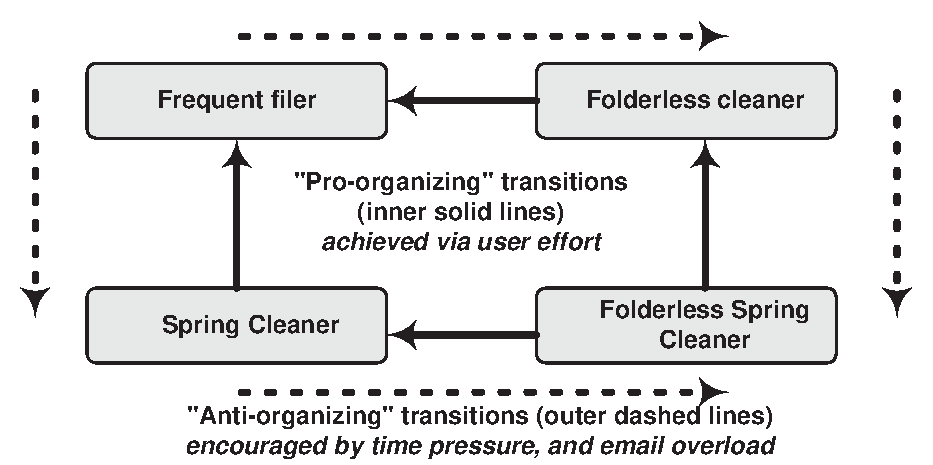
\includegraphics[width=.7\textwidth]{pictures/research_review/Ch2-BalterLongitudinalModel.pdf}
	\end{center}
	\caption{Model of changes in email management strategy over time~\citep{ob:97}}
	\label{fig:ch2_balter_model}
\end{figure}


%%%%%%%%%%%%%%%%%%%%%%%%%%%%%%%%%%%%%%
% \subsection{Descriptive Frameworks}
%%%%%%%%%%%%%%%%%%%%%%%%%%%%%%%%%%%%%%
%% Refer to as descriptive frameworks?
%% Highlight import of context, and information is used? 
% Trends in HCI theory have been described as a \textit{turn towards the social}~\citep{rogers:04}. Several theoretical methods, heavily influenced from sociology have been taken up by HCI researchers including Distributed Cognition and Activity Theory.
%%%%%%%%%%%%%%%%%%%%%%%%%%%
% DISTRIBUTED COGNITION
%%%%%%%%%%%%%%%%%%%%%%%%%%%
Distributed Cognition (DC) is a theoretical framework which has been used to model cognitive processes distributed across time, space and multiple actors, e.g. aircraft carrier control rooms~\citep{dc:00}.
%%%%%%%
% DIX
%%%%%%%
Two sets of descriptive terminology have been proposed to describe the functions provided by items and tools in the user's personal information environment.  \citet{dix:98} offers a conceptual framework describing the function of items in supporting user activities.  He identifies two key concepts: (1) \textit{triggers}, items such as reminders that can initiate action, and (2) \textit{placeholders} which are arrangements of items which can maintain task state allowing it to be restarted at a later time.  A second, more abstract set of terminology is offered by~\citet{dk:01}.  Kirsh reports a theoretical analysis of an information environment as an activity space within which the user carries out their tasks.  He proposes a number of theoretical constructs to describe the conceptual structures that users project onto the environment: (1) \textit{entry points} (cues to start tasks), (2) action landscapes (arrangements of items that support a particular activity), and (3) coordinating mechanisms (artefacts such as calendars that allow the user to perform multiple activities).  \citet{Whittaker-rta:00} note the need for the community to agree on standardized descriptive terminology as a stepping stone to developing predictive theories.  The above frameworks represent the first steps towards establishing agreed terminology in this area.  % although at an early stage of development, represent important progress in this direction.  

% However it is not clear how such descriptive frameworks would be applicable to design and would probably suffice as a stepping stone towards further research.
% offers a theoretical analysis of PIM, considering the PIM-system as distributed between an individual and their environment. Kirsh describes how user and their PIM environment co-evolve over time, and 
%%%%%%%%%%%%%%%%%%%%%%%%%%%%%%%%%%%%%%%%%%%%%%%%%%
% Existing theory is focused on storage+retrieval
%%%%%%%%%%%%%%%%%%%%%%%%%%%%%%%%%%%%%%%%%%%%%%%%%%
% Current task descriptions of PIM are focused on the traditional perspective of storage for future retrieval. There is also a need for theory to handle contextualizing functions of personal information management such as reminders, and task management.

%%%%%%%%%%%%%%%%
% KAPTELININ
%%%%%%%%%%%%%%%%
% Activity Theory -- A conceptual framework, not predictive or cookbook in terms of design. Basic principles: object relatedness, hierarchical structure of activity (activities (motives), actions (goals), operations (conditions)), internalization/externalization, mediation, development.
% \citep{Kaptelinin:03} applies an another theoretical framework to PIM: Activity Theory~\citep{bn-at:95}. He performs an analysis of a user's activities in which personal information is used. The theoretical analysis is used to provide design rationale for the \textit{UMEA} system.
% Distributed Cognition and Activity Theory may prove useful as conceptual frameworks to define a descriptive vocabulary for personal information management. 



%%%%%%%%%%%%%%%%%%%%%%%%%%%%%%%%%%%%%
\subsubsection{Predictive Models}
\label{review:theory-pimmodels-predictive}
%%%%%%%%%%%%%%%%%%%%%%%%%%%%%%%%%%%%%
% However, two models of email usage have been proposed. \citet{Whittaker-email:96} propose a simple \textit{one-touch} model of inbox processing: that items are opened, read and then immediately filed or deleted.  They acknowledge that this is inaccurate since studies, including their own observe users keeping many messages for later processing.
%%%%%%%%%%%%%%%%%%%%%%%
% PREDICTIVE MODELS
%%%%%%%%%%%%%%%%%%%%%%%
% However his findings have been countered by recent empirical findings that suggest that many experienced users develop , a strategy which Balter indicates is inefficient. % The model can be criticised for not encompassing filters and other realistic aspects of information management.
% Furthermore, the model relies of . Users will expend more time and effort storing information which is highly valued. It is therefore in their interest to structure the information environment so as to make frequently accessed information easy to find.  The question remains can purely economic considerations be used to predict user behaviour. All these models are founded on the premise that information is stored for later retrieval. Other aspects of information management such as reminding are not encompassed.
Few predictive models of PIM behaviour have been developed.  One exception is that of \citet{ob:00} who proposes a keystroke-level model of email archiving and retrieval.  Based on the model, Balter issues prescriptive advice to tool designers and to users with respect to optimizing their behaviour in terms of time efficiency.  Balter's model can be criticised for its reliance on economic costs of information access and storage.  For example, one of Balter's claims is that any strategy involving more than 30 folders is inefficient.  Studies of email usage have observed highly experienced email users with large numbers of folders~\citep{Ducheneaut:01}.  Such findings suggest that either Balter's model is inaccurate, or that there is more at stake than time efficiency in dictating choice of management strategy.  Factors such as the need for tidiness, or the placement of items as reminders are not captured within the model.  However, Balter's work should be acknowledged as a first step in generating prescriptive advice in this complex area.

%%%%%%%%%%
% PAYNE
%%%%%%%%%%
% Payne~\citep{sp:93} carried out a cognitive-artifact analysis on personal calendar usage. He observed how people employ multiple calendar artefacts but typically rely on paper calendars. Payne states that electronic calendars, even though often used for collaborative scheduling, should be treated by developers as personal artefacts.


%%%%%%%%%%%%%%%%%%%%%%%%%%%%%%%%%%%%%%%%%%%%%%%%%%%%%%%%%%%%%%%%%
%% Typical criticism:  use to illustrate research-practice gap}
%%%%%%%%%%%%%%%%%%%%%%%%%%%%%%%%%%%%%%%%%%%%%%%%%%%%%%%%%%%%%%%%%

%%%%%%%%%%%%%%%%%%%%%%%%%%%%%%%%%%%%%%%%%%%%%%%
\subsection{Models of Information Retrieval}
\label{review:theory-pimmodels:ir}
%%%%%%%%%%%%%%%%%%%%%%%%%%%%%%%%%%%%%%%%%%%%%%%
% Other references - see Weiss-Lijn thesis
%%%%%%%%%%%%%%%%%%%%%%%%%%%%%%%%%%%%%%%%%%%%%%%

%%%%%%%%%%%%%%%%%%%%%%%%%%%%%%%%%%%%%%%%%%
% general intro on information retrieval
%%%%%%%%%%%%%%%%%%%%%%%%%%%%%%%%%%%%%%%%%%
% (AKA information-seeking or information-foraging) 
\textbf{Section~\ref{bg:pim-relatedterms}} highlighted how information retrieval is a key aspect of PIM.  Theories from information retrieval may be useful to the developers of more general PIM-related theories.

% Firstly, it relates to the retrieval of items from a user's PIM system. Secondly it relates to the retrieval of information from remote information systems to include in a user's PIM system. An example of this would be downloading a document from the web and saving a local copy. \textbf{Section\ref{bg:pim-relatedterms}} discusses the relationship between information retrieval and personal information management.
%%
%% relate to earlier discussion on relationship between PIM and other areas}. Reference diagram. 
%%
% As such information retrieval should be considered as a lower-level process than personal information management, but one which is complex in itself. An information retrieval system has been defined as \textit{an information retrieval system does not inform (i.e. change the knowledge of) the user on the subject of his inquiry. It merely informs on the existence (or non-existence) and whereabouts of documents relating to his request}~\citep{Rijsbergen:79}. Information retrieval is guided by the notion of an information need. The ongoing process of PIM will encompass many distinct information retrieval events.
%% 
%% IR lower level than PIM -- one aspect of PIM, also focus has mainly been GIS rather than PIS. But NB: complex in itself.
%%%%%%%%%%%%%%%%%%%%
% USeful for PIM
%%%%%%%%%%%%%%%%%%%%
% Information retrieval is a field with its own conferences and journals and is generally much more mature than personal information management. Reasons for this are discussed below. Theories from information retrieval may be useful to the developers of PIM-systems. Examples are discussed below.


%%%%%%%%%%%%%%%%%%%%%%%%%%%%
% information foraging
%%%%%%%%%%%%%%%%%%%%%%%%%%%%

\textit{Information Foraging (IF)}~\citep{pirolli:99} is a theory that supports the construction of computational models of information-seeking behaviour.  The theory is based on evolutionary theories of survival, leading to the premise \textit{``that information systems evolve towards a stable state of maximising the transfer of valuable information per unit cost''}.  Users will seek to follow an optimal strategy so as to achieve this.  Three activities are considered: (1) enrichment, (2) scent following, and (3) exploitation.
% NB: users won't necessarily follow an optimal strategy though
The models encompasses a notion of information value in terms of information scent, and the cost of interaction (e.g. mouse clicks). % The ACT-IF model has been used to simulate behaviour in a scatter/gather prototype.
IF theory has been most recently applied to website design.


%%%%%%%%%%%%%%
% Sutcliffe
%%%%%%%%%%%%%%
% An alternative approach is employed by Ennis \& Sutcliffe~\citep{sutcliffe:98} who present a cognitive model of information retrieval



%%%%%%%%%%%%%%%%%%%%%%%%%%%%%%%%%%%%%%%%%%%%%%
% \subsection{Models of Information behaviour}
%%%%%%%%%%%%%%%%%%%%%%%%%%%%%%%%%%%%%%%%%%%%%%
% Generally information science has been more focused on information retrieval than other aspects of PIM.
% Wilson criticises this over-focus and presents a more encompassing theory of information behaviour. This is discussed in the next section.
% which is typically left unspecified in the information retrieval literature.
\citet{wilson:99} observes that many models of information retrieval do not encompass how that information is used, beyond the general notion of an \textit{information need}.  He proposes a general model of information behaviour that encompasses information retrieval and other aspects of information usage.  However, the model does not capture aspects of PIM such as how information may be stored and organized over time.








%%%%%%%%%%%%%%%%%%%%%%%%%%%%%%%%%%%%%%%%%%%%%%%%
\subsection{Personal Classification Schemes}
\label{review:theory-classificationschemes}
%%%%%%%%%%%%%%%%%%%%%%%%%%%%%%%%%%%%%%%%%%%%%%%%

%%%%%%%%%%%%%%%%%%%%%%%%%%%%%%%
% Studies of classification
%%%%%%%%%%%%%%%%%%%%%%%%%%%%%%%
%%%%%%%%%%%%%%%%%%%%%%%%%%%%%%%%%%%%%%%%%%%%%%
%% Other stuff from classification science
%%%%%%%%%%%%%%%%%%%%%%%%%%%%%%%%%%%%%%%%%%%%%%
%% Personal versus Shared ontologies~\citep{shapiro:99}. Messes~\citep{abrahamson:02}
%% Has it been applied? 
% , a cognitive process that is applied during the organizing material in semantic or spatial categories.
% Borges~\citep{borges:62} highlights the need for classification -- to deal with the complexity of the world (cognitive economy).  
% The second relevant body of basic science relates to the cognitive process of classification.. Cognitive psychology and classification science offer many findings on the workings of human classification processes.
\textbf{Chapter~\ref{chapter:bg}} noted that most current PIM-tools are centred on a hierarchical classification mechanism.  This section surveys some theory on classification, before describing criticisms that have been levelled at the folder hierarchy.

The folder hierarchy allows the user to specify a classification scheme within which items can be categorized. \citet{bs:99} define a classification scheme as \textit{``a spatial, temporal or spatio-temporal segmentation of the world''}. They propose three theoretical properties of a classification scheme: (1) a consistent, unique classificatory principle, such as temporal or alphabetical ordering, (2) mutually exclusive categories, and (3) completeness. However, as they note, no real-world classification is this ideal -- classificatory principles often contradict, categories overlap, and many items cannot be categorized (hence the use of catch-all categories such as ``stuff'').

Many theories of classification have been developed through the ages. The Classical Theory originated with Plato in Ancient Greece~\citep{ek:90}.  
%% summarised in Margolis and Laurence 1999.
The Classical Theory states that the cognitive concepts on which categories are based carry their own definitional structure. Categorizing an item is thus the process of matching its features against those of the concept. In recent years the Classical Theory has been subjected to intense criticism, and other views such as Prototype Theory~\citep{er:78} have come to the fore. Prototype Theory states that a category is a statistical representation of the
properties that its members tend to have, i.e. each category is represented by an exemplar. Under Prototype Theory, categorizing an item involves comparing it to each category's exemplar. Rosch identifies two basic principles that influence the formation of categories: (1) cognitive economy (classification is about providing maximum information about the world for the least cognitive effort), and (2) perceived world structure (categories are based on the high correlational structure possessed by the attributes of real-world objects).  These two principles have implications for the level of abstraction of categories formed in a category system (inclusiveness), and the internal structure of those categories once formed (prototypes).

Classification schemes can be considered as a means of cognitive scaffolding~\citep{jacob:01} -- they allow people to deal with the complexity of large systems. % Jacob identifies two types of classification scheme: personal and infrastructural. Infrastructural classification schemes are developed by an organization or society, whilst personal classification schemes are developed by an individual.
%% ADD EXAMPLE
%% YUCK - TIDY THIS
~\cite{ob:00} describes the retrieval-time benefits from organizing in terms of "reducing the search space". Instead of scanning a long list of unstructured items, users can home in on a particular subset directly.

% In contrast to pre-defined structures, a personal classification scheme allows the user to create an individualised organization, customized to their way of thinking and working. The user may choose to create categories based on whichever organisational dimensions  that they see as relevant (e.g. role, project or time). Categories can be represented in various ways, depending on the classificatory mechanism in use.  A typical desktop workspace might contain categories in the form of a cluster of icons at a spatial location, emails contained within a folder labelled semantically with a text string, or a set of hypertext links on a personal web page.

% Our electronic workspaces contain a wide range of personal classification schemes. Common examples in desktop workspace include the folder hierarchies of the file system, mail tools and web browsers for organising documents, messages and web links respectively. Resources may also be organized spatially as an arrangement of icons on the desktop. Many software packages also contain their own specific hierarchies for organising specialized types of informationsuch as source code, images and music files. Some operating systems contain their own idiosyncratic hierarchies, such as the Start Menu of Microsoft Windows that is used to organise software tools and access recently accessed documents. Workspace itself may be organized in terms of virtual windows assigned to a flat category space~\cite{rooms:86}.

%%%%%%%%%%%%%%%%%%%%%%%%%%%%%%%%%%%%%%%
% HOW TO APPLY TO REAL-WORLD DESIGN?
%%%%%%%%%%%%%%%%%%%%%%%%%%%%%%%%%%%%%%%
%%  not really theory of PIM but provide foundation for much of the design work.
%% How have findings been used? Have any been used beyond general ad-hoc scientific grounding
% The question remains over whether findings from objective lab studies relating to low-level cognitive processes involved in personal information management such as recall, recognition and classification can offer useful guidance for designers developing tools for use in the real world.  % Lansdale~\citep{ml:92} makes design suggestions drawn from the basic findings such as providing the user with multiple retrieval cues.
% However, it not clear how such low-level principles can be made relevant to designers.  The research has been useful however in terms of documenting the basic cognitive capabilities of users.    

			
%%%%%%%%%%%%%%%%%%%%%%%%%%%%%%%%%%%%%%%%%%%%%%%%%%%%
\subsubsection{Limitations of the Folder Hierarchy}
%%%%%%%%%%%%%%%%%%%%%%%%%%%%%%%%%%%%%%%%%%%%%%%%%%%%%
%%%%%%%%%%%%%%%%%%%%%%%%%%%%%%%%%%%%%%%
%% Rationalize with stuff in Chapter 2
%% Is this designer intuition or actual theory?
%%%%%%%%%%%%%%%%%%%%%%%%%%%%%%%%%%%%%%%
%% Also: Ad-hoc categories.
%% Limits of such anecdotal commenary. NB: usually accompanies non-evaluated revolutionary prototype.
% Many research prototypes have been motivated by intuitive technological arguments.
Hierarchies are the standard computational mechanism used to define personal classification schemes~\citep{dourish:99a}. They are both easy to program and familiar to most users. However, 
a number of criticisms have been levelled at the hierarchy, e.g. ~\citep{nielsen:96,bell:02,tn:99,Gelernter:96a,dourish:99a,jr:00}
\footnote{Similar arguments against hierarchical schemes have also been made in other domains such as architecture. \citet{alexander:65} argues that a hierarchical city layout is not a good match for the dynamic and interleaved nature of human activity.}.
One fundamental limitation is that of \textit{single-inheritance}~\citep{nielsen:96,dourish:99a}, i.e. an item may only be filed in one place. Most operating systems provide mechanisms to override single-inheritance in
the form of links (UNIX), aliases (MacOS) or short-cuts (Windows) but they often confuse users~\citep{dourish:99a}. Furthermore, hierarchies have also been criticized for their static nature, and for poor scalability to large information spaces.

%% ADD THE FOLLOWING BACK IN?
%% Structuring items into categories also impedes the use of implicit
%metadata. Chronological information is an example of a organizing principle
%often used by individuals to organize various types of personal information
%such as bookmarks and email. 


%%%%%%%%%%%%%%%%%%%%%
% DEFENSE OF TREE
%%%%%%%%%%%%%%%%%%%%%	
% Further discussion is provided in \textbf{Section~\ref{bg:pimtool-cf}}.
%% CHECK THIS 
%% Large amount of non-rigorous (mainly) insubstantiated postering. Attack and (little) defense of the hierarchy.	  Summarize main points
%% Interject with defense of the tree here? Why is the tree so dominant?
%% Andy Hertzfeld quote -- tree as totally fundamental
%% Add \textbf{Claims analysis} of the tree?
The question of why the traditional folder hierarchy continues to dominate PIM-systems is an interesting one.  Alternatives offering more flexibility have been available for over a decade, e.g.~\citep{semanticfs:91}.  The key technological advantage of the tree is that it is simple and easy to implement.  Although the above criticisms have had a profound influence in design, questions remain over whether they are confirmed by user data.  For instance, ~\citet{bn:95} report that the participants in their study were satisfied with their folder organizations and had little need for multiple classification. This suggests that the hierarchy, despite its limitations, has the benefits of being an organizational paradigm which users are broadly satisfied and familiar with. % Also it offers a positive constraint of knowledge domain and participant~\citep{jacob:01}, persistence, and the ability to assign multi-attributes in one go.






%%%%%%%%%%%%%%%%%%%%%%%%%%%%%%%%%%%%%%%%%%%%%%%%%%%%%%%%%%%%%%%%%%%%%%%
\subsection{Discussion of Theoretical Contributions}
\label{theoretical-contribution-discussion}
%%%%%%%%%%%%%%%%%%%%%%%%%%%%%%%%%%%%%%%%%%%%%%%%%%%%%%%%%%%%%%%%%%%%%%%
%%%%%%%%%%%%%%%%%%%%%%%%%%%%%%%%%%%%%%%%%
% WHY DO WE WANT THEORY ANYWAY?
%%%%%%%%%%%%%%%%%%%%%%%%%%%%%%%%%%%%%%%%%
% What would such theory be useful for? 
% Theoretical discussions and models (can they explain data?) -- types of theory: descriptive, explanatory, prescriptive, generative etc. Lack of encompassing theory and frameworks
% Newman:  Why not appropriate for PIM tools? 
%%%%%%%%%%%%%%%%%%%%%%%%%%%%%%%%%%%%%%%%
% Issue: how to be useful for design
%%%%%%%%%%%%%%%%%%%%%%%%%%%%%%%%%%%%%%%%
%% Key issues: applicability, scalability.
%% Retouch the Theory/Practice Gap
% Too low-level: other cognitive models. Why?~\citep{ml:92}
% Medium-level but not relevant: information-seeking, information-foraging
% Too high-level: descriptive frameworks. Consider use of AT as an approach.


%%%%%%%%%%%%%%%%%
% BOTTOM LINE
%%%%%%%%%%%%%%%%%
% Theory tends to work at the extremes: low-level cognitive phenomena, or high-level collaborative scale
% Bodies of theory are identified from other areas which may be applicable. 
% there is a lack of coherenmt theory of PIM.  Instead, 
% no coherent theory of PIM. In general theory tends to be very low-level (cognitive scale) or very high-level (descriptive theory).
This section confirms the observation of \citet{Whittaker-rta:00}, that there is a lack of theoretical foundation for PIM, despite its status as a fundamental computer-based activity.  % A range of theoretical work to PIM has been surveyed. 

\citet{Whittaker-rta:00} highlight the need for standardized descriptive vocabulary as a first step towards developing more powerful predictive theories that can provide principled advice to designers, and dictate design characteristics.  Conceptual frameworks such as those described in \textbf{Section~\ref{review:theory-pimmodels}}, have made some progress in this area, but there is clearly much more to be done.
% , there is 
% Theory from information retrieval could for example be applied to model retrieval from personal information management systems. However some higher-level framework is required to tie retrieval and storage together, along with acquisition and maintenance.

% \textit{A ``devils advocate'' argument is provided by advocates of the empiricist perspective on HCI  (Landauer etc.): that much HCI behaviour is too complex to predict/design from theory. Instead, they advocate  use alternative of iterative requirements-gathering, design and evaluation and treat designed artefacts as theory~\citep{Carroll-cycle:91}.} % This perspective on HCI theory is discussed in more detail in \textbf{Section~\ref{hci-state}}.

\citet{rogers:04} outlines a number of properties of effective HCI theories, that highlight the kind of theory needed in this area.   Firstly, the theory should \textit{scale} to an appropriate granularity of task.  However, much HCI theory is focused at a low-level on the cognitive, perceptual, and motor function systems~\citep{newman:95}.  In the context of PIM, cognitive theories of human memory and classification may not be applicable to  modelling natural real-world classification decisions in a hectic work environment~\citep{ml:92}. Other theory is very high-level, such as the conceptual frameworks offered by~\citet{dk:01}.  One route may be to combine theories which focus on different levels of analysis~\citep{barnard:00}.   Secondly, theory must be \textit{applicable}.   The challenge for theorists is to develop models that can be useful in a design context.  It is not clear how much of the existing body of theoretical work is of practical help to designers.
% A meta-theory could try and relate low-level cognitive processes involved in one-off storage and retrieval decisions (medium-level) to other high-level long-term user activities.


%%%%%%%%%%%%%%%%%%%%%%%%%%%%%%%%%%%%%%%%%%%%
% Relevance to integration in particular
%%%%%%%%%%%%%%%%%%%%%%%%%%%%%%%%%%%%%%%%%%%%
% Since there is no theory applicable to a single PIM-system, it follows that there is none relevant to inter-tool integration. A first step may be to develop appropriate descriptive vocabulary. Whittaker \textit{et al}.~\citep{Whittaker-rta:00} argue that for effective theory-building you first need more empirical groundwork to achieve consensus on task description, and descriptive vocabulary.

% Little theory exists that is directly applicable to PIM-integration/unification.
% No coverage in particular of issues relating to multiple tools and integration.


%%%%%%%%%%%%%%%%%%%%%%%%%%%%%%%%%%%
% Alternative approach to theory
%%%%%%%%%%%%%%%%%%%%%%%%%%%%%%%%%%%
% May be a better approach since so much design out there in the real world. Create theory to establish why these tools work as well as they do. And furthermore a theoretical baseline for dealing with observed problems.

% %%%%%%%%%%%%%%%%%%%%%%%%%%%%%%%%%
% FIGURE - Coverage of Theories
%%%%%%%%%%%%%%%%%%%%%%%%%%%%%%%%%%%
% \begin{figure}[t]
%	\begin{center}
%		\leavevmode
%		
\includegraphics[height=2in, width=.9 \textwidth]{pictures/research_review/Ch2-TheoryCoverage.pdf}
%	\end{center}
%	\caption{Coverage of theories}
%	\label{fig:chapter2_theory_coverage}
%\end{figure}

	
%%%%%%%%%%%%%%%%%%%%%%%%%%%%%%%%%%%%%
%% \subsubsection{Directions for future theoretical research}
%%%%%%%%%%%%%%%%%%%%%%%%%%%%%%%%%%%%%%

%%%%%%%%%%%%%%
% SIGNPOSTING
%%%%%%%%%%%%%%%
% This section reviewed the third research area identified in \textbf{Section~\ref{review:pim-research-overview}}: theory relevant to PIM software. It is concluded that little theory exists in the area for design guidance. Some basic theory can be built on in terms of developing a descriptive framework. The next section draws together work presented in this section and the two previous ones to present a view on the overall state of research concerned with personal information management.



%%%%%%%%%%%%%%%%%%%%%%%%%%%%%%%%%%%
%%%%%%%%%%%%%%%%%%%%%%%%%%%%%%%%%%%
%%%%%%%%%%%%%%%%%%%%%%%%%%%%%%%%%%%
%%%%%%%%%%%%%%%%%%%%%%%%%%%%%%%%%%%

\newpage
%%%%%%%%%%%%%%%%%%%%%%%%%%%%%%%%%%%%%%%%%%%%
%%%%%%%%%%%%%%%%%%%%%%%%%%%%%%%%%%%%%%%%%%
\section{Discussion} %  of Prior Research}
\label{review:discussion}
%%%%%%%%%%%%%%%%%%%%%%%%%%%%%%%%%%%%%%%%%%
%%%%%%%%%%%%%%%%%%%%%%%%%%%%%%%%%%%%%%%%%%%%
% phrase: used to argue the potential
% Emphasise theory/practice gap
% PIM has surged ahead of theory (i.e. its a successful application)
%% HCI left behind
% Tone down critcisms and frame as `open research questions'
%%%%%%%%%%%%%%%%%%%%%%%%%%%%%%%%%%%%%%%%%

%%%%%%%%%%%%%%%
% SIGNPOSTING
%%%%%%%%%%%%%%%
%summarizes key limitations of previous work, and motivates 
%, before a focus is taken on research concerned with integration.
%portrayed as a break in the Task-Artefact cycle. Recommendations for future research are proposed.
This section draws together the three areas of research -- empirical studies, design and theory -- discussed in \textbf{Sections~\ref{review:pim-empirical-review}}, \textbf{~\ref{review:pim-technological-review}}, and \textbf{~\ref{review:pim-theory-review}}.  The overall state of HCI knowledge concerned with the PIM application domain is summarized in \textbf{Section~\ref{review:discussion:critical-analysis}}.  Limitations in the area of PIM-integration are identified, and used to motivate the thesis research agenda in \textbf{Section~\ref{review:research-agenda}}.  Finally, \textbf{Section~\ref{review:methodology}} details the selection of methodology for the thesis.


%%%%%%%%%%%%%%%%%%%%%%%%%%%%%%%%%
\subsection{Critical Analysis of Previous Research}
\label{review:discussion:critical-analysis}
%%%%%%%%%%%%%%%%%%%%%%%%%%%%%%%%%
%% SUMMARY: frame situation within PIM-research (creation of a systematic knowledge base) as a break in the task-artefact cycle. Emphasis: reuse}.
% empirical-contribution-discussion
% Thus researchers starting work in the field need to start work from scratch. 
% Whittaker \textit{et al}. argue that this basic groundwork is essential for the development of theory in the area. 
In this chapter, two main engines of research progress have been identified: \textit{empirical studies} and \textit{technology design}. However, despite the body of previous work in each area, the author echoes the affirmation by~\citep{Whittaker-rta:00} that PIM has not received the attention it merits as a fundamental computer-based activity.  In terms of empirical studies, \textbf{Section~\ref{empirical-contribution-discussion}} highlighted a lack of attention to longitudinal aspects of PIM, and to the needs of non-technical users.  \citet{Whittaker-rta:00} argue that this insufficient empirical grounding has contributed to the lack of consensus on descriptive vocabulary, task decompositions, evaluation metrics, or the key problems that need to be solved.  

\textbf{Section~\ref{technological-contribution-discussion}} surveyed previous technological prototyping in the research domain, with a particular focusing on that offering increased PIM-integration.  Two key problems were highlighted.  Much of this body of work can be criticised in terms of making a strong contribution to the HCI knowledge base due to: (1) a lack of grounding in empirical requirements, and (2) a lack of evaluation. This situation can be portrayed as a \textit{break in the task/artefact cycle}~\citep{Carroll-cycle:91}. Studies of user practices are not providing firm grounding for design, which is in turn not being systematically evaluated.

% When evaluation and requirements exist they have been inconsistent and therefore it is hard to compare between designs. It is also observed that existing methods are very application-focused and enforce compartmentalization. %% tidy this waffle

%%%%%%%%%%%%%%%%%%%%%%%%%%%%%
% WHY POOR EPISTEMIC STATE
%%%%%%%%%%%%%%%%%%%%%%%%%%%%%
% Secondly PIM is a hard phenomenon to study. It is long-term and highly idiosyncratic meaning that traditional methods of cognitive-model based analysis such as GOMS are not applicable. Generally there is a lack of theory to build on, and a lack of appropriate evaluation methods. 
Several reasons can be suggested for this poor epistemic state. Firstly, PIM may be seen as ``an area of old technology''.  \citet{Carroll-review:97} discusses the strong research interest on collaborative technology, and the author speculates that PIM may seem a backward, unchallenging area to some researchers.  Secondly, there is a lack of theory and methodology concerning complex high-level activities such as PIM.  \citet{ad:01} and \citet{Whittaker-rta:00} note the lack of appropriate evaluation metrics for evaluating PIM designs. For instance, traditional measures of usability may be inappropriate for evaluating interfaces that support discretionary activities such as PIM.  Thirdly, PIM is a multi-faceted, ongoing, and highly idiosyncratic activity, and may be seen as too challenging an area.  Perhaps this explains the much larger amount of work carried out towards the lower-level area of information retrieval.   In the meantime, progress in developing PIM technology in the commercial arena, is out-stripping the level of knowledge in the research community.  This phenomenon is not specific to PIM and has been termed the \textit{research/practice gap}~\citep{Carroll:00,rogers:04}.  % in the software development arena far out-strips that in HCI, and the evaluation of innovative PIM-tools is left to the market-place (for example no published research on Windows Longhorn~\citep{winfs:03} has appeared).

% One suggested route forward has been proposed by~\citet{Whittaker-rta:00}.  They call for the refocusing of research around \textit{reference tasks}, core everyday tasks such as those involved in PIM.  They describe how such a research focus has proved useful in other research fields.  They call for the definition of tyasks, descriptive vocabulary, task decomposition into main components, metrics for evaluation. This would allow objective comparison of different interaction techniques and enable systematic theory development.

%% Summarise as broken task/artefact cycle Use Task/Artifact Cycle~\citep{Carroll-cycle:91,jc-cycle:92} as a perspective - cycle broken
%%%%%%%%%%%%%%%%%%%%%%%%%%%%%%
% OVERALL: LACK OF ATTENTION
%%%%%%%%%%%%%%%%%%%%%%%%%%%%%%

%%%%%%%%%%%%%%%%%%%%%%%%%%%%%%%%%%%%%%%%%%%%%%%
\subsection{Research Agenda}
\label{review:research-agenda}
%%%%%%%%%%%%%%%%%%%%%%%%%%%%%%%%%%%%%%%%%%%%%%%

% Much has been written on HCI's recent turn \textit{towards the social}, e.g.  \textit{``The portrait of a solitary user finding and creating information in a computer became background to the portrait of several people working together at a variety of times and places''}~\citep{Carroll-review:97}.  Although the recent trend \textit{towards the social} has opened up many interesting areas for research, it has also contributed towards many core everyday computer-based activities such as PIM being under-researched~\citep{Whittaker-rta:00}.  

Turning the pages of recent HCI conferences reveals a wealth of current research directed at collaborative and social interfaces, and other ``cutting edge'' areas such as virtual reality and intelligent agents, but very little on important everyday activities such as PIM.  This thesis seeks to help readdress this balance by taking a conscious turn back towards fundamental, everyday user problems.  After surveying the field, the author developed a particular interest in the problems caused by a user's information being fragmented across a set of distinct PIM-tools.  The PIM-integration genre has attempted to provide solutions to these problems by providing functionality which bridges multiple tools.  However, as noted above, much of this work can be criticised for: (1) a lack of evaluation, and (2) insufficient empirical grounding.

% One area of particular interest to the researcher is the PIM-integration design genre, which has attempted to deal with 

% in the other direction, away from collaborative activities back towards the individual user and a focus on the most personal of activities, PIM.  
% careful PIM: has collaborative aspects


%%%%%%%%%%%%%%%%%%%%%%%%
% ORIENTING INTERESTS
%%%%%%%%%%%%%%%%%%%%%%%%
% The author's initial interests which he brought to the research are described before the initial research objectives are presented.
%%%%%%%%%%%%%%%%%%%%%%%%
% Interest in DESIGN
%  As well as the general interest in integration, another key interest of the author was in design -- in actually implementing the fruits of his research in a concrete artefact which could then be evaluated. 
%% Need to pursue integration-design in an incremental manner, need for requirements, 
%% Balance what I want to do with what is pragmatically possible (what I'm best-equipped to do)

%%%%%%%%%%%%%%%%%%%%%%%%%%%%%%%%%%
% \subsection{Objectives}
%%%%%%%%%%%%%%%%%%%%%%%%%%%%%%%%%%

%%%%%%%%%%%%%%%%%%%%%%%%%%%%
% AIMS/GOALS/OBJECTIVES
%%%%%%%%%%%%%%%%%%%%%%%%%%%%
% Guided by the interests described above, and building on the limitations of previous work in the area of improving integration -- the research was inherently cross-tool: i.e. not focused on a specific application.
% The thesis objectives are defined as follows: (1) to build on current understanding, (2) to provide guidance for designers.
This high-level aim of this research programme was to provide guidance for the designers of PIM-integration mechanisms.  Three key research objectives were identified:
\begin{enumerate}

%%%%%%%%%%%%%%%%%%%%%%%%%%%%%%%%%%%%%%%%%%%%%%%%%%%%%%%%%%%%%%%%%%
% EMPIRICAL : Objective 1: To build on current understanding}
%%%%%%%%%%%%%%%%%%%%%%%%%%%%%%%%%%%%%%%%%%%%%%%%%%%%%%%%%%%%%%%%%%
% Requirements for design.
% provide evidence/description
% Under-researched. Accept observations of relative lack of attention that PIM has received to date within HCI and take steps towards alleviating it. Need for more understanding of core phenomena. Emphasise grounding in empirical data. Empirical stance adopted
% % There is a lack of understanding of fundamental everyday computer-based activities  such as PIM. Importance of grounding in user experiences with the current generation of PIM artefacts (concern for ecological validity).  Understand the world. Study real practice. Use to develop understanding of PIM. 
%%%%%%%%%%%%%%%%%%%%%%%%%%%%%%%%%%%%%%%%%%%%%%%%%%%%
% The first objective was to provide improved understanding of personal information management, with a particular focus on investigating user needs and issues relating to integration between PIM-tools.
%%%%%%%%%%%%%%%%%%%%%%%%%%%%%%%%%%%%%%%%%%%%%%%%%%%%
%%%%%%%%%%%%%%%%%%%%%%%%%%
% ENVISAGED CONTRIBUTION
% The planned method to achieve this objective was to carry out a cross-tool study. The study would provide increased cross-tool understanding of PIM, and so provide an empirical foundation for cross-tool design work aimed at improving PIM integration.
%%%%%%%%%%%%%%%%%%%%%%%%%%%%%%%%%%%%%%%%%%%%%%%%%%%%
\item \textit{To develop increased understanding of PIM behaviour and user needs} -- In order to provide a firm empirical foundation for PIM-integration design work, the author planned to investigate user behaviour and needs beyond the boundaries of specific tools.
%%%%%%%%%%%%%%%%%%%%%%
% LEAD -> THEORETICAL
%%%%%%%%%%%%%%%%%%%%%%%
A secondary aim was to develop theoretical models to describe and explain empirical observations.


%%%%%%%%%%%%%%%%%%%%%%%%%%%%%%%%%%%%%%%%%%%%%%%%%%%%%%%%%%%%%%%%%%%%%%%%%%
% DESIGN/EVALUATION : Objective 2: To provide guidance for designers}
%%%%%%%%%%%%%%%%%%%%%%%%%%%%%%%%%%%%%%%%%%%%%%%%%%%%%%%%%%%%%%%%%%%%%%%%%%%%%
% improved tool support for PIM.
% \textit{The author embarked on the work with a strong interest in design, and a background in engineering, which lead to the intention to create an interactive artefact. Commitment to simplifying?  Interest in non-professional/non-technical users?~\citep{web-good-easy:01}}
% Propose technology and evaluate, contrast with more ambitious programs to revolutionize the desktop.
% To design and evaluate new PIM technology in practice (real users, real data, real tools, real environment, over time). Artefact generation. Yet need to do so systematically and contribute to HCI knowledge-base.
%%%%%%%%%%%%%%%%%%%%%%%%%%%%%%%%%%%%%%%%%%%%%%%%%%%
% THE OBJECTIVE
% The second objective was to produce a set of design recommendations regarding the design of improved PIM tools, particularly design work aimed at improving PIM integration.
% This objective was to be achieved through design/evaluation experience.
% The intention was to use findings from the initial study to form grounded design rationale to direct the design.
%%%%%%%%%%%%%%%%%%%%%%%%%%%%%%%%%%%%%%%%%%%%%%%%%%%
% THE METHOD
%%%%%%%%%%%%%
% Due to the lack of appropriate methodology, a parallel aim was to explore issues related to the evaluation of PIM tools, particularly those aimed at improving PIM integration. 
%%%%%%%%%%%%%%%%%%%%%%%%%%%%%%%%%%%%%%%%%%%%%%%%%%%
\item \textit{To propose, implement and evaluate an empirically-grounded means of PIM-integration} -- The author embarked upon the research programme with a keen interest in developing a novel PIM-integration mechanism.  A key interest was to improve upon the limitations of previous design-centred research, by emphasising empirical grounding and evaluation, and thus making a more systematic contribution to HCI knowledge.
% However, in contrast to most previous design work in the area, the intention was t
 
 %%%%%%%%%%%%%%%%%
% METHODOLOGICAL
%%%%%%%%%%%%%%%%%
% Methodological: Explore potential of cross-tool approach for both researchers and designers of cross-tool approach. Evaluation: explore ways of doing effective evaluation.  To explore issues related to the evaluation of PIM designs, particularly those directed at improving PIM integration.
% regarding appropriate methodology
% devise appropriate methodology to support the above objectives of investigating PIM, and designing and evaluating PIM-integration mechanisms.  Furthermore, based on these experiences, to produce a set of recommendations regarding the design of PIM interfaces, particularly those aimed at improving PIM integration.
\item \textit{To devise methodological recommendations for future research and design work } -- The final objective was to provide methodological guidance for future work in the area of PIM-integration (and PIM more generally), based on the experience gained in pursuing this course of research.  \citet{Whittaker-rta:00} note the lack of appropriate methodology such as evaluation metrics.

\end{enumerate}

% The next section discusses the methodological approach employed in the thesis to achieve the above objectives.


%%%%%%%%%%%%%%%%%%%%%%%%%%%%%%%%%%%%%%%%
\subsection{Selection of Methodology}
\label{review:methodology}
%%%%%%%%%%%%%%%%%%%%%%%%%%%%%%%%%%%%%%%%
% This section collates a summary of the methods used in personal information management research. These findings are used to justify the selection of methods used in this thesis.
% Previous empirical work has mostly been based on an ethnomethodological approach, although objective studies have also been carried out -- mostly in terms of task-specific evaluations of new designs. There is no agreed understanding of core problems.
%% \item Requirements gathering: Studies -- ethnographic/fieldwork techniques. Main engine.
% Theory-building based on empirical data has been rare and there has is no agreed methodological approach. In some ways this is consistent with the state of affairs in HCI.
%% Theory-building: Cognitive modelling~\citep{ob:00}. Rare.
% There is no generally accepted design methodology, or approach for describing design rationale.
% Design methods remain controversial in terms of design rationale. 
%In general the design work has been radical/revolutionary, whilst incremental (evolutionary, cumulative) design work is seen as more scientific by many researchers such as Kuhn~\citep{newman:95,Carroll:00}. In some cases design has been based on specific empirical findings~\citep{Bellotti:00,Bellotti:03,bn:98}. The author is not aware of any collaborative design being carried out in the area. In other cases it has been based on specific theoretical principles~\citep{ml:92}. However the majority of design work has been based on designers' intuition and anecdotal reports of user problems. This is not a problem in itself, however the additional lack of evaluation is.
% There is clearly scope for theory to guide design work and further studies.However it has been noted that HCI is not well equipped with appropriate techniques for dealing with PIM.  For example, Dillon~\citep{ad:01} notes the lack of appropriate evaluation methodology for evaluating interfaces that support discretionary activities (activities with no immediate goal) such as PIM.  Suggested approaches include \textit{Reference Tasks} - limiting context to a specific user-group/tool/task such as information retrieval~\citep{Whittaker-rta:00}.  But there are inherent limitations in focusing on one sub-task in this way, when one considers the inter-relationship between the different aspects of PIM - e.g. retrieval and previous organization.  %% THIS NEEDS TIDYING
%%%%%%%%%%%%%%
% Evaluation
%%%%%%%%%%%%%% In addition, there is no consensus on evaluation metrics~\citep{Whittaker-rta:00}. This means that in those cases where evaluations have been carried out, it is hard to compare between designs. In many cases, evaluations have not been performed at all.
%% What other methodological lessons have been learned? e.g. Import of individual differences

Methodology has been defined as \textit{``something that avoids you having to think too hard about how to do something''}~(anon.). % However the lack of methodological consensus in the area means that the author had to think very hard about how to do everything!
%%%%%%%%%%%%%%%%%%%%%%%%%
% Classic HCI dilemma
%%%%%%%%%%%%%%%%%%%%%%%%%
However, the selection of appropriate research methodology is a classic HCI dilemma.  As an interdisciplinary research field, HCI offers many research approaches and methodologies~\citep{Sasse:97}.
%%%%%%%%%%%%%%%%%%%%%%%%%%%%%%%%%%%%%%%%%%%%%%%%%%
% Selection of design-centered methodology
%%%%%%%%%%%%%%%%%%%%%%%%%%%%%%%%%%%%%%%%%%%%%%%%%%
% , chosen as it matches the two \textbf{orienting commitments} of this research:
% Blomberg et al.~\citep{blomberg:96} similarly advocate a design-centred approach through two complementary commitments design and research to support each other and improve~\citep{blomberg:96}.
% Design-based research is selected as an appropriate methodology to enable the candidate to experience design issues at first hand. Turn towards design science route. Promise of design-based research methodology. Subscribe to design-based research methodology. Outline how to do research by this approach. Outline how to add to HCI KB according to~\citep{jc:00}. Recap pros and cons and how I will account for them.
%% A view that my research takes up with gusto.  Need to get hands dirty
The methodology employed in this thesis is heavily influenced by the \textit{design-based} research paradigm, as advocated in~\citet{Carroll:00}.  Carroll describes how design can be employed as a research method to achieve two complementary goals: (1) to \textit{understand the world} through the process of gathering design requirements, and (2) to \textit{improve the world} by creating a new artefact.  He contrasts this applied research paradigm (literally ``research through design'') with traditional perspectives on design as a \textit{craft}, or design as \textit{the object of research}.  Carroll argues how the designed artefact can be interpreted as a theory, a set of claims regarding how a particular situation of concern can be improved.  Theory development, the validation of the designers' claims, is enabled through the subsequent evaluation of the design, a crucial stage of the research process.  This assessment of the strengths and weaknesses of a specific design may then be generalizable to a wider design genre. The task-artefact cycle~\citep{Carroll-cycle:91} forms a backdrop to the research approach: the study of a task context provides the requirements for the design of an artefact, which is then in turn evaluated in the context of the original task.  Evaluation also provides an opportunity for further empirical discovery (understanding of the world).


% The evaluation of the tool then enables further investigation of the nature of the activity.
% The end-product of the research is the designed artefact itself, grounded in its empirical and theoretical motivation, and post-design evaluation.

%%%%%%%%%%%%%%%%%%%%%%%%%%%%%%%
% APPROPRIATENESS OF APPROACH
%%%%%%%%%%%%%%%%%%%%%%%%%%%%%%%
% A key concern in HCI is the so-called \textit{theory/practice gap} (or research/practice gap)~\citep{Sutcliffe:00,rogers:04}.  There is concern that the products of much HCI research may be irrelevant to HCI practitioners who pursue their craft without need for theory or strict methods. 
% The traditional view of research is that theory leads practice, 
% in reality often not the case. In many cases design leads whilst theory catches up over time.
The approach was seen to be highly compatible with the author's desire to produce a novel PIM-integration mechanism, whilst also supporting the exploration of user behaviour, and theoretical development.  Also, it was envisaged that by experiencing design issues at first hand, the author was more likely to produce findings in a form of relevance to practitioners. % . A key concern in HCI is the so-called \textit{theory/practice gap} (or research/practice gap)~\citep{Sutcliffe:00,rogers:04}, whereby the products of much HCI research can be irrelevant to designers' needs in the real-world.


% Therefore In this paradigm, research is performed through a standard iterative-design process: the investigation of user needs to establish design requirements, the design of interactive artefacts to meet those needs, and the evaluation of the design in real-world use. 



%%%%%%%%%%%%%%%%%%%%%%%%%%%%%%%%%%%%%%%%%%%%%%%%%%%%%%%%%%%%
%% NB: need to make case for the selected research method
%%%%%%%%%%%%%%%%%%%%%%%%%%%%%%%%%%%%%%%%%%%%%%%%%%%%%%%%%%%%
%% Make the case for my chosen methods. The choice of methods to be employed in the research are outlined. The main approaches to HCI research in general are discusseda above. Prior HCI research methods employed in the PIM application domain are surveyed. 
%%%%%%%%%%%%%%%%%%%%%%%%%%%%%%%
% \subsubsection{Research Methodology}
%%%%%%%%%%%%%%%%%%%%%%%%%%%%%%%
%%%%%%%%%%%%%%%%%%%%%%%%%%%%%%%%%%%%%%%%%%%%%%
% Walkthrough the stages of the methodology
%%%%%%%%%%%%%%%%%%%%%%%%%%%%%%%%%%%%%%%%%%%%%%
% employs a 3-stage , centered on a process of user-centred design~\citep{} consisting of three stages: (a) an exploratory study, (b) design work, (c) follow-up evaluation and further study.
% The selected method is a design-based research methodology and can be considered as an instance of standard HCI practice~\citep{Whittaker-rta:00}: (1) interviews users to understand needs, (2) develop system to meet needs, and (3) evaluate it to see if it meets those needs.
\newpage
Specifically, the research reported in subsequent chapters is centred on a 3-stage \textit{user-centred design} methodology:

\begin{enumerate}

%%%%%%%%%%%%%%
% FIRST STAGE
%%%%%%%%%%%%%%
%, managed within the file system, email tool, and web browser respectively.
% DIANE: not too much detail here
% Tio provide evidence/description
% Requirements will be gathered through a cross-tool study to build cross-tool understanding of PIM, and so provide an empirical foundation for cross-tool design work aimed at improving PIM integration. The study methodology will consist of semi-structured interviews as used in previous empirical work in this area. The aim is to compare how individuals manage a range of types of personal information, to investigate the effectiveness of current forms of integration, and so as support the generation of empirically-grounded ideas of how further integration can be provided.
\item \textit{Requirements gathering} -- The research is empirically grounded in an exploratory study, reported in \textbf{Chapter~\ref{chapter:exploratory_study}}.  The study was aimed at both developing more understanding of PIM, and establishing requirements for subsequent design.  % \textbf{Chapter~\ref{chapter:exploratory_study}} details the study which compares PIM practices across 3 collections of personal information: personal files, email, and web bookmarks. 

%%%%%%%%%%%%%%%%%%
% SECOND STAGE
%%%%%%%%%%%%%%%%%%
\item \textit{Design and prototyping} -- Findings from the exploratory study are used to motivate the design and implementation of a prototype PIM-integration mechanism in \textbf{Chapter~\ref{chapter:design}}. In order to facilitate systematic evaluation, and cause minimum disruption to users, the design route is \textit{incremental} rather than revolutionary~\citep{newman:95}. % The prototype was proposed as a research vehicle to enable the investigation of general issues relating to PIM integration during a field study.
% The design was prototyped so as to embody specific design hypotheses that express intended improvements.
% The findings from the exploratory study will provide the grounding for the design of an interface providing enhanced PIM integration. 
% the design may be a new form of integration or modify an existing form
%% contrast with unification systems that unify and propose a new organizational paradigm. I just do one

%%%%%%%%%%%%%%%%%%
% THIRD STAGE
%%%%%%%%%%%%%%%%%%
\item \textit{Evaluation} -- \textbf{Chapter~\ref{chapter:main-study}} reports the field-study based evaluation of the prototype. \citet{ml:92} notes the importance of evaluating PIM technology over time. As well as evaluating the proposed design, the field study also enabled the investigation of long-term user behaviour such as changes in strategy over time. 
% Note that the field study also facilitates the investigation of long-term aspects of PIM such as changes in strategy over time. Such longitudinal aspects of PIM have received little attention to date.
% Since no evaluations of this type have been carried out, an important part of this work is the development of appropriate methodology, both for evaluating PIM-tools in general, but also for evaluating means of integration.
% Finally the main study also allowed the investigation of appropriate methodology for evaluating PIM tools.
% Do these really go together? Maybe bring out in the discussion - rather than as an up-front aim!
% Finally the effectiveness of the design will be investigated through a field study-based evaluation.
%% to assess impact of the design intervention

% \item The iterative process of study, design and evaluation provided a platform for theory-building.

\end{enumerate}

% This three-step research agenda will be portrayed as an excursion around the task-artefact cycle. \textbf{Section~\ref{review:discussion}} discusses how much previous PIM research breaks this cycle.
% The next section summarizes the work presented over subsequent chapters, and details the research contributions offered.





%%%%%%%%%%%%%%%%%%%%%%%%%%%%%%%%%%%%%%%%
%\subsection{Justification of Methodology}
%\label{review:methodology}
%%%%%%%%%%%%%%%%%%%%%%%%%%%%%%%%%%%%%%%%
%In this section, recommendations are made for future direction in research into personal information management.
% Personal information management is considered in general, before the section focuses on research into improving integration between PIM-tools.
%%%%%%%%%%%%%%%%%%%%%%%
% Interest in INTEGRATION
%%%%%%%%%%%%%%%%%%%%%%%
%At an early stage, the author expressed an interest in design efforts aimed at improving integration between PIM-tools. A lack of integrated, applicable body of knowledge on integration was identified in much of this chapter. There is a lack of descriptive vocabulary for discussing such technology, and its usage has not been researched. An initial conceptual framework was presented in \textbf{Chapter~\ref{chapter:bg}} but this is clearly just a first step.
% be more specific
%The majority of \textbf{Section~\ref{review:pim-technological-review}} was devoted to a survey of this work, much of which can be criticized for a lack of empirical/theoretical foundation and a lack of evaluation.  Several steps were identified in \textbf{Section\ref{review:research-recommendations}} for making progress in this area.
%The promise of new technology in this area from the commercial sector means that artefacts in use will continue to move beyond continued research understanding. This is an important area of user activity that needs increased and more systematic research understanding to guide future design work.
%In conclusion, four recommendations are made by the author to enable HCI research to provide more effective knowledge to designers seeking to improve \textit{integration} between PIM tools in a more scientific way: 
%\begin{enumerate}
%\item A descriptive vocabulary must be defined so that different forms of integration can be described using consistent terminology. This goes hand in hand with the theoretical groundwork talked about by Whittaker \textit{et al}. and discussed above.
%\end{enumerate}
%%%%%%%%%%%%%%%
% SIGNPOSTING
%%%%%%%%%%%%%%%
% This section summarized the current state of research and outlined areas for improvement. \textbf{Section~\ref{intro:aims}} sets out a research agenda for this thesis within this context. % Here, \textbf{Section~\ref{review:conclusion}} concludes the chapter and states the contributions towards the overall thesis.
%% Moving on towards how I can take a step towards this in my PhD ...

%%%%%%%%%%%%%%%%%%%%%%%%%%%%%%%%%%%
% \newpage
%%%%%%%%%%%%%%%%%%%%%%%%%%%%%%%%%%%%%%%%%%%%%%%%%%%%%%%
%%%%%%%%%%%%%%%%%%%%%%%%%%%%%%%%%%%%%%%%%%%%%%%%%%%%%%
% MOVED-TO/MERGED-WITH CHAPTER 1
%\section{A Research Agenda for this Thesis}
%\label{review:research-agenda}
%%%%%%%%%%%%%%%%%%%%%%%%%%%%%%%%%%%%%%%%%%%%%%%%%%%%%%
%%%%%%%%%%%%%%%%%%%%%%%%%%%%%%%%%%%%%%%%%%%%%%%%%%%%%%%
%% MOVING ON: emphasise huge area, need to focus}


%%%%%%%%%%%%%%%%%%%%%%%%%%%%%%%%%%%
%%%%%%%%%%%%%%%%%%%%%%%%%%%%%%%%%%%
%%%%%%%%%%%%%%%%%%%%%%%%%%%%%%%%%%%
%%%%%%%%%%%%%%%%%%%%%%%%%%%%%%%%%%%
% \newpage
%%%%%%%%%%%%%%%%%%%%%%%%%%%%%%%%%%%
%\section{Conclusion}
%\label{review:conclusion}
%%%%%%%%%%%%%%%%%%%%%%%%%%%%%%%%%%%
%In this section conclusions from \textbf{Chapter~\ref{chapter:review}} are presented. 
% Contributions include a critical review of the literature and the analysis of key limitations, a taxonomy of PIM technology design research relating to integration, and the presentation of recommendations for future research in the area. Analysis of limitations of previous research lead to the development of the initial thesis objectives presented in \textbf{Section~\ref{intro:aims}}.
% \textbf{Chapter~\ref{chapter:exploratory_study}} presents an exploratory study of personal information management, the first step on that research agenda.

\textbf{Chapter~\ref{chapter:exploratory_study}} now moves on to report the first stage of the design-centred methodology employed in this thesis, an exploratory study that compares how people manage three types of personal information: files, email and bookmarks.

%%%%%%%%%%%%%%%%%%%%%%%%%%%%%%%%%
% FIN THESIS CHAPTER 3: LITREVIEW
%%%%%%%%%%%%%%%%%%%%%%%%%%%%%%%%%
% \textit{This draft of Chapter 3 LITREVIEW was printed \today}


% %%%%%%%%%%%%%%%%%%%%%%%%%%%%%

% chapter 4 - Exploratory Study

% %%%%%%%%%%%%%%%%%%%%%%%%%%%%%

\chapter{Exploratory Cross-tool Study}

\label{chapter:exploratory_study}

% \textit{CHAPTER 4 LEFT INTENTIONALLY BLANK AS A PLACEHOLDER}


%%%%%%%%%%%%%%%%%%%%%%%%%%%%%%%
% CHAPTER 4: EXPLORATORY STUDY
%%%%%%%%%%%%%%%%%%%%%%%%%%%%%%%
%% INTRODUCTION
%%%%%%%%%%%%%%%%%%%%%%%%%%%%%%%%%%%%%%%%%%%%%%%
%%%%%%%%%%%%%%%%%%%%%%%%%%%%%%%%%%%%%%%%%%%%%%%%
\section{Introduction}
\label{exp-study:introduction}
%%%%%%%%%%%%%%%%%%%%%%%%%%%%%%%%%%%%%%%%%%%%%%%%
%%%%%%%%%%%%%%%%%%%%%%%%%%%%%%%%%%%%%%%%%%%%%%%%

%%%%%%%%%%%%%%%%%%%%%%%%%%%%%%%%%%%%%%%%%%%%%
% ABBREVIATIONS
% SP SIGNPOSTING
%%%%%%%%%%%%%%%%%%%%%%%%%%%%%%%%%%%%%%%%%%%%%
% SECTION TODOs
% * Fix section references to earlier chapters
% * THINK: can I structure relative to CF?
%%%%%%%%%%%%%%%%%%%%%%%%%%%%%%%%%%%%%%%%%%%%%
% CONTENT
% Add as driver QUESTION: do results hold across multiple tools?
% Tone down critcisms and frame as `open research questions'
%%%%%%%%%%%%%%%%%%%%%%%%%%%%%%%%%%%%%%%%%%%%%

%%%%%%%%%%%%%%%%%%%%%%%%%%%%%%%%%%%%%%%%%%%%%%%%%%
% CHAPTER INTRO
% * bang bang bang intro, straight into aims - MUST BE PERSUASIVE
% * Need to relate Chapter aims to Thesis aims
%%%%%%%%%%%%%%%%%%%%%%%%%%%%%%%%%%%%%%%%%%%%%%%%%%
% \footnote{This draft of Chapter 4 Exploratory cross-tool study was printed \today}
% Twenty-five participants were interviewed over the period from from Autumn 2000 to Summer 2002.
% This \textit{cross-tool} perspective goes beyond previous work by allowing the construction of a cross-tool profile of user behaviour.  
% \textbf{Chapter~\ref{chapter:exploratory_study}}
% It was envisaged that such cross-tool data would provide guidance for the design of PIM-tool integration mechanisms.
This chapter reports an exploratory study of everyday Personal Information Management (PIM) practices.  A key objective of this study was to develop a holistic understanding of participants' PIM behaviour by collecting data across three PIM-tools: files, email and bookmarks. The study's cross-tool scope differentiates it from most previous studies in the area which have focused on specific PIM-tools (see \textbf{Section~\ref{review:pim-empirical-review}}).
% In contrast, previous studies have focused on \textit{specific} PIM-tools such as email (e.g.~\citep{Whittaker-email:96}, 
\textbf{Figure~\ref{fig:exp-study:intra_versus_cross_tool}} compares previous \textit{tool-specific} studies, with the the \textit{cross-tool} approach employed here.
% These two perspectives, tool-specific and cross-tool, are compared in  The tool-specific approach as employed in previous studies allows the \textit{within-tool/between-users} characterization of PIM practices within particular tool.  In contrast the cross-tool approach employed here enabled the comparison of practices between tools.    % This cross-tool nature of the study reported here allowed the comparison of behaviour between different PIM-tools. 
%%%%%%%%%%%%%%%%%%%%%%%%%%%%%%%%%%%%%%%%%%%%%%%%%%%%%%%%%%%%%%%%%%%%%%%%%%
% Describe the two cross-tool analysis approaches
% (1) comparison of generalized/aggregate data AND (2) within-user profile
%%%%%%%%%%%%%%%%%%%%%%%%%%%%%%%%%%%%%%%%%%%%%%%%%%%%%%%%%%%%%%%%%%%%%%%%%%
% In this study, cross-tool analysis was carried out from two perspectives: (1) comparing generalized behaviour, aggregated across all participants, and (2) comparing practices between tools for specific users. More detail is provided on each perspective below.
% The first perspective involved the comparison of \textit{generalized} behaviour between the three PIM-tools. To cover all aspects of PIM, interviews were structured to cover Barreau's four PIM sub-activities in each collection.  This analytical perspective is equivalent to carrying out three tool-specific studies in parallel. In the chapter, a novel technique is proposed to compare the tools in terms of the \textit{organizational dimensions} used to name folders in each PIM-tool.
%%%%%%%%%%%%%%%%%%%%%%%%%%%%%%%
% between-tools/within-user
%%%%%%%%%%%%%%%%%%%%%%%%%%%%%%%
% The second perspective involved \textit{between-tools/within-user} analysis to compare PIM practices across all three tools for each participant. A novel technique is presented to construct a \textit{cross-tool profile} for each participant in terms of the extent to which they organized multiple types of information.  This contrasts with previous strategy profiling which has only been carried out in the context of specific tools.
% A second technique is proposed to assess the similarity of folder structures in different PIM-tools based on the level of \textit{folder overlap}.
% Finally the cross-tool profiles were categorized to develop a classification of cross-tool PIM practices across all participants.
% Three new analytical techniques were employed in the study: analysis of \textit{organizational dimensions}, \textit{cross-tool profiling} and analysis of \textit{folder overlap}.

% %%%%%%%%%%%%%%%%%%%%%%%%%%%%%
% FIGURE - Intra-tool/Cross-tool Comparison
% %%%%%%%%%%%%%%%%%%%%%%%%%%%%%
\begin{figure}[hbtp]
	\begin{center}
		\leavevmode
		% height=2in, width=.9 \textwidth
		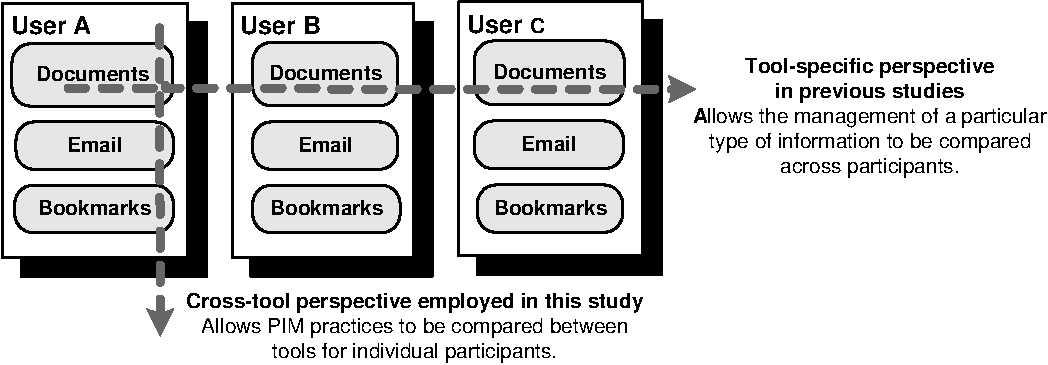
\includegraphics[height=4cm]{pictures/exp-study/exp-study-intracrosscomparison.pdf}
		\caption{Comparing the cross-tool and tool-specific study perspectives.} 	% The two analytical perspectives used in PIM studies: (1) tool-specific (within-tool/between-users); and (2) cross-tool (between-tools/within-user).}
		\label{fig:exp-study:intra_versus_cross_tool}
	\end{center}
\end{figure}

%%%%%%%%%%%%%%%%%%
% LINK FORWARDS
%%%%%%%%%%%%%%%%%%
% This section details the chapter's contributions towards the overall thesis.
% This chapter acts as an empirical foundation for the rest of the thesis.
The findings in this chapter, combined with the insights reported in \textbf{Chapter~\ref{chapter:review}}, provide an empirical grounding for the design work in \textbf{Chapter~\ref{chapter:design}}.
% Lessons learned in carrying out the exploratory study also help shape the methodology employed in the subsequent empirical work reported in \textbf{Chapters~\ref{chapter:design}} and \textbf{\ref{chapter:main-study}}.
% The study also contributed to the development of the cross-tool analytical framework outlined in \textbf{Chapter~\ref{chapter:discussion}}.
The work presented in this chapter has been reported in a number of publications ~\citep{rpb:01b,rpb:02c,rpb:03a,rpb:04a}.


%%%%%%%%%%%%%%%%%%%%%%%%%%%%%
% LINK TO REST OF SECTION
%%%%%%%%%%%%%%%%%%%%%%%%%%%%%
% The rest of this section is structured as follows. Firstly \textbf{Section~\ref{exp-study:objectives}} presents the study's objectives. Then \textbf{Section~\ref{exp-study:study-scope}} reports decisions made to limit the study's scope of inquiry. \textbf{Section~\ref{exp-study:contributions}} discusses the chapter's contributions towards the overall thesis.  

%%%%%%%%%%%%%%%%%
%%%%%%%%%%%%%%%%%
%%%%%%%%%%%%%%%%%
%%%%%%%%%%%%%%%%%

%%%%%%%%%%%%%%%%%%%%%%%%
\subsection{Objectives}
\label{exp-study:objectives}
%%%%%%%%%%%%%%%%%%%%%%%%

The study objectives were as follows:
\begin{enumerate}

%%%%%%%%%%%%%%%%%%%%%%%%%%%%%%%%%%%%
% OBJECTIVE 1: Cross-tool Knowledge
%%%%%%%%%%%%%%%%%%%%%%%%%%%%%%%%%%%%%%%%%%%%%%%%%%%%%%%%%%%%%%%%%%%%%%%%%%%%%%%%%%%%%%%%%%%%%%%%%%%%%%%%%%%%
% FROM CHI04: Although many innovative designs have been proposed, WE see a mismatch between the tool-specific studies that have provided observations about users� activities and problems � and the substantial design effort directed at cross-tool integration. There is a need for cross-tool empirical data to provide a foundation for such cross-tool design.
% FROM CHI04: Our study aimed to build on previous research in two ways: 1.	
%%%%%%%%%%%%%%%%%%%%%%%%%%%%%%%%%%%%%%%%%%%%%%%%%%%%%%%%%%%%%%%%%%%%%%%%%%%%%%%%%%%%%%%%%%%%%%%%%%%%%%%%%%%%
% NB: consider exceptions, eg CM, TKM
%%%%%%%%%%%%%%%%%%%%%%%%%%%%%%%%%%%%%%%%%%%%%%%%%%%%%%%%%%%%%%%%%%%%%%%%%%%%%%%%%%%%%%%%%%%%%%%%%%%%%%%%%%%%
%% To provide a cross-tool empirical foundation for the thesis by investigating participants' PIM practices across three collections of information: files, email, and bookmarks. 
% and to develop a rich picture of PIM behaviour across a range of tools.
% To provide a more effective foundation for cross-tool design, WE profiled participants' practices in  It was envisaged that cross-tool data would be useful in establishing an empirically-grounded foundation 
%% In particular a key motivation behind this research programme was an interest in exploring the potential to improve integration between PIM tools. \textit{Thus the above high-level objectives should be considered in the context of this interest.} 
%%%%%%%%%%%%%%%%%%%%%%%%%%%%%%%%%%%%%%%%%%%%%%%%%%%%%%%%%%%%%%%%%%%%%%%%%%%%%%%%%%%%%%%%%%%%%%%%%%%%%%%%%%%%
\item	\textit{To compare how users manage different types of personal information} -- \textbf{Section~\ref{review:pim-technological-review}} identified a mismatch between the \textit{tool-specific} empirical studies that have provided observations about PIM behaviour and problems, and the substantial \textit{cross-tool} design effort directed at improving integration between PIM tools.  Furthermore, it was argued that much of this design work has been based on designer intuition rather than empirical data.  A case was made for more cross-tool empirical data to provide an effective empirical foundation for the design of integration mechanisms. % surveyed the substantial design effort that has been directed at improving integration between PIM tools. 

The primary aim of this study was to take steps towards addressing this research gap.  To achieve this, participants' PIM practices were profiled across three commonly managed collections of personal information: (1) document files, (2) email messages and (3) web bookmarks -- managed within the file system, email tool and web browser respectively. 

%%%%%%%%%%%%%%%%%%%%%
% OBJECTIVE 2: Design foundation
%%%%%%%%%%%%%%%%%%%%%
%   By developing understanding of PIM from a cross-tool perspective, it was envisaged that the study would provide requirements and ideas for subsequent design work.
\item \textit{To provide motivation and requirements for subsequent design} -- An orienting commitment in this research was to design and evaluate a novel PIM-integration mechanism.  It was hoped that the study findings would guide subsequent design work. % within this programme of research.

%%%%%%%%%%%%%%%%%%%%%%%%%%%%%%%%%%%%
% OBJECTIVE 2: General knowledge including tool-specific knowledge
%%%%%%%%%%%%%%%%%%%%%%%%%%%%%%%%%%%%
%%%%%%%%%%
% NOTES
% * need base understanding in specific tools to build up cross-tool understanding
% * change to familiarise himself?
% * Mention fact that do not discuss individual PIM-tools in depth, for this see previous studies.
%%%%%%%%%%%%
\item	\textit{To provide background on PIM} -- \textbf{Chapter~\ref{chapter:review}} highlights the lack of a systematic knowledge base of empirical data relating to PIM.   In addition to building up a \textit{cross-tool} understanding of PIM, the study was seen as an opportunity for the author to ``get his hands dirty'' and familiarise himself with a range of PIM-related issues, e.g. those relating to specific PIM-tools.
% develop a first-hand appreciation of user needs.
% author hoped to ,   In general, the study was seen as an opportunity for the author 

%%%%%%%%%%%%%%%%%
% OBJECTIVE 3: Research focus
%%%%%%%%%%%%%%%%%
\item \textit{To confirm a research focus} -- Since PIM is a complex activity and offers a wide range of compelling research problems (see~\textbf{Chapter~\ref{chapter:introduction}}), the author perceived a strong need to focus his research efforts.  % NB: fix section reference
The exploratory study was intended to help identify an interesting, worthwhile and achievable research problem. % i.e. justify research focus

\end{enumerate}

%%%%%%%%%%%%%%%%%
%%%%%%%%%%%%%%%%%
%%%%%%%%%%%%%%%%%
%%%%%%%%%%%%%%%%%

%%%%%%%%%%%%%%%%%%%%%%%%%%%%%%%
\subsection{Study scope}
\label{exp-study:study-scope}
% \textbf{Section~\ref{exp-study:studyscope}} 
%%%%%%%%%%%%%%%%%%%%%%%%%%%%%%%
% This section details the decisions taken by the author to limit the study scope.
% \textbf{Chapter~\ref{chapter:bg}} outlines the complex nature of PIM as an idiosyncratic, ongoing activity made up of four key sub-activities (acquisition, organization, maintenance and retrieval). The challenges inherent in investigating such a long-term, multifaceted activity, were compounded by the intention to investigate PIM across a range of tools. 
% One consequence of widening the scope of enquiry to encompass multiple tools is that the complexity of the HCI phenomena being investigated is increased. 
% Faced with the potential of such analytical complexity, the following constraints were applied to limit the study's scope:
%%
%% \footnote{\textit{NOTE TO READERS OF DRAFT: \textbf{Figure~\ref{fig:chapter1_pim_model}} is included at the end of this section to illustrate the analytical framework that I use for talking about PIM (based on that of~\citep{barreau:95}). Note that in the final version this conceptual grounding will be located in the introductory chapter}}.
The primary aim of the study, to investigate a complex activity such as PIM from a holistic, \textit{cross-tool} perspective, was clearly an ambitious one.  In order to offset the potential analytical complexity, the scope of the study was constrained in the following ways:

\begin{enumerate}

%%%%%%%%%%%%%%%%	
% SCOPE LIMIT 1
%%%%%%%%%%%%%%%%
% : the primary desktop workspace
\item \textit{Focus on PIM practice within the context of a single personal computer} -- The domain of interest was limited to the computer where each participant performed the majority of their computer-based activity at their place of work. Thus the extra complexity of considering PIM on multiple computers and mobile devices was avoided.

%%%%%%%%%%%%%%%%
% SCOPE LIMIT 2
%%%%%%%%%%%%%%%%
% digital and physical tools to manage personal information 
% Fix figure reference ~\ref{fig:chapter1_workspace}}). 
\item \textit{Focus on three PIM-tools} -- Even within the context of one computer, users often employ a wide and varying range of PIM-tools (see \textbf{Figure~\ref{fig:chapter2_pie}}). 
Due to time constraints, it was decided to focus the study on three commonly-used PIM-tools: files, email and web bookmarks.  A further focus was taken on the management of \textit{personal document files} within the file system, as described in \textbf{Section~\ref{exp-study:interview-process}}.
% Although the core of the study focused on these three collections, enquiries were made regarding other PIM tools (e.g. address books and calendars) if time allowed.

%%%%%%%%%%%%%%%%
% SCOPE LIMIT 3
%%%%%%%%%%%%%%%%
\item \textit{Non-longitudinal study} -- As noted in \textbf{Chapter~\ref{chapter:review}}, PIM is an ongoing activity, and user behaviour may evolve over time~\citep{ob:97}.  However, due to time constraints, and likemost previous studies, this investigation was based on a one-off ``snapshot'' of behaviour\footnote{In the exploratory study, it was still possible to collect data relating to longitudinal issues (e.g. changes in strategy) in the form of historical reports offered by participants.  \textbf{Chapter~\ref{chapter:main-study}} reports a follow-up longitudinal study carried out by the author that captured data over time.}.

%%%%%%%%%%%%%%%%
% SCOPE LIMIT 4
%%%%%%%%%%%%%%%%
 % For example the members of a team may each store personal information in a shared email account or within a sub-folder on a network drive.
%% THINK: this small print can be encapsulated in definition in Background chapter
%% Such as: what are the extra issues concerned with collaborative information management
% cite Collaborative Information Management issues (e.g. Berlin et al. 1993)
\item \textit{Focus on personal rather than shared information} -- As noted in \textbf{Chapter~\ref{chapter:bg}}, a user may store personal information within a group information space, such as a network drive shared with colleagues. To avoid taking into account the issues related to collaboration, this study focused on information that was not shared with other users.

\end{enumerate}

%%%%%%%%%%%%%%%%%
%%%%%%%%%%%%%%%%%
%%%%%%%%%%%%%%%%%
%%%%%%%%%%%%%%%%%


	





%%%%%%%%%%%%%%%%%%%%%%%%%%%%%%%%%%%%%%%%%%%%%%
\subsection{Contributions}
\label{exp-study:contributions}
% \textbf{Section~\ref{exp-study:contributions}}
%%%%%%%%%%%%%%%%%%%%%%%%%%%%%%%%%%%%%%%%%%%%%%

The following methodological and substantive contributions are offered in the chapter:
%% NB: for all of these, must relate to SO WHAT?
% The first set of substantive contributions resulted from the \textit{within-tool/between-users} analysis. ALSO CONSIDER: SO WHAT!!
% (perspective 1 in~\textbf{Figure~\ref{fig:chapter3_intra_versus_cross_tool}}):
\begin{enumerate}

%%%%%%%%%%%%%%%%%%%%%%%%%%%%%%%%%%%%%%%%%%%%%%%
% CONTRIB B: COMPARISON OF STRATS IN TOOLS
%%%%%%%%%%%%%%%%%%%%%%%%%%%%%%%%%%%%%%%%%%%%%%%
% by capturing data across multiple tools for each participant
% The second set of substantive contributions result from the \textit{between-tools/within-user} analysis:
% ADD: SO WHAT: Implications are discussed in XYZ
% The study's primary contribution is in terms of \textit{improved cross-tool understanding of PIM}. A high-level comparison of management strategies is presented in \textbf{Section~\ref{exp-study:Results-comparison}} to contrast behaviour between the file, email, and bookmark collections across all the participants.
% This initial cross-tool comparison is based on the generalized views of user behaviour developed in the \textit{within-tool/between-user} analysis.
% The cross-tool analysis is used to derive a set of design implications for improving tool integration.
\item \textit{A comparison of PIM behaviour between the three PIM-tools} -- \textbf{Section~\ref{exp-study:Results-comparison}} presents a high-level comparison between files, email and bookmarks in terms of four PIM sub-activities (acquisition, organization, maintenance and retrieval).  This data emphasises how the nature of PIM varies between different PIM-tools.


%%%%%%%%%%%%%%%%%%%%%%%%%%%%%%%%%%%%%%%%%%%%%%%%%%%%%%%%%%%%%%
% CONTRIB E: NEW METHOD OF C/T PROFILING AND APPLICATION
%%%%%%%%%%%%%%%%%%%%%%%%%%%%%%%%%%%%%%%%%%%%%%%%%%%%%%%%%%%%%%
% A method of performing the cross-tool profiling of users. The method is applied here to illustrate the variation in terms of extent of filing across tools for many participants. Evidence of multiple strategies at a cross-tool level for many people.
\item \textit{A comparison of organizing strategies between the three PIM tools} -- A focus is taken on the organizing sub-activity in \textbf{Section~\ref{exp-study:Results-org-strategies}}, where it is observed that many individuals employ a rich variety of organizing strategies \textit{both within and across PIM tools}.  Previous classifications of organizing behaviour are criticised for not reflecting this behaviour, and new classifications are offered for tool-specific and cross-tool contexts.  
% \textbf{Section~\ref{exp-study:discussion:multiple-strategies}} presents a model to describe the observations of multiple strategies in tool-specific and cross-tool contexts.
% The second methodological contribution is that of \textit{cross-tool profiling}. 
% A classification of PIM behaviour is presented to indicate the extent of user's organizing across multiple tools.

%%%%%%%%%%%%%%%%%%%%%%%%%%%%%%%%%%%%%%%%%%%%%%%%%%%%%%%%%%%%%%
% CONTRIB C: NEW METHOD OF ORG DIM ANALYSIS AND APPLICATION
%%%%%%%%%%%%%%%%%%%%%%%%%%%%%%%%%%%%%%%%%%%%%%%%%%%%%%%%%%%%%%
% \item An new method and application of analysis of the organizational dimensions used to name folders in each tool. This is used to criticise PIM-integration based on one organizational dimension.
% (the types of concept, e.g. people, projects, places on which folder names are
\item \textit{The development and application of a novel technique for comparing the organizational dimensions on which folders are based in each PIM-tool} -- Organizational dimensions are defined as the types of concept on which folder names are based (e.g. project or interest).  The method employed is described in \textbf{Section~\ref{exp-study:folder-analysis-orgdim}}.  The results in \textbf{Section~\ref{exp-study:Results-org-dims}} highlight the range of dimensions employed by users to name folders in the three PIM-tools. A number of previous PIM-integration systems are criticised for focusing on one type of organizational dimension.

%%%%%%%%%%%%%%%%%%%%%%%%%%%%%%%%%%%%%%%%%%%%%%%%%%%%%%%%%%%%%%
% CONTRIB D: NEW METHOD OF F/O ANALYSIS AND APPLICATION
%%%%%%%%%%%%%%%%%%%%%%%%%%%%%%%%%%%%%%%%%%%%%%%%%%%%%%%%%%%%%%
\item \textit{The development and application of a novel technique for assessing the similarity of a user's file, email and bookmark folder structures in terms of overlapping folders} -- The method is documented in \textbf{Section~\ref{exp-study:analysis-folder-overlap}}, and results are presented in \textbf{Section~\ref{exp-study:Results-folder-overlap}}. Significant folder overlap is observed for most study participants, particularly between their file and email collections.  These results provide a key design motivation for the WorkspaceMirror tool presented in \textbf{Chapter~\ref{chapter:design}}.
% Folder overlap is proposed as a means of assessing the similarity of two structured collections of personal information.
% A new method and application of analysis of the extent of folder overlap between the tools

%%%%%%%%%%%%%%%%%%%%%%%%%%%%%%%%%%
%  SUBSTANTIVE 6: General implications for design
%%%%%%%%%%%%%%%%%%%%%%%%%%%%%%%%%%
\item \textit{Implications for the design of PIM-integration mechanisms} -- \textbf{Section~\ref{exp-study:comparison-problems}} highlights a range of cross-tool problems highlighting the potential of improving integration between PIM-tools.  \textbf{Section~\ref{exp-study:conclusion}} presents a number of design implications for improving tool integration, based on the findings in the chapter. 
% The cross-tool findings are used to argue for possible routes for integrating between tools, see \textbf{Section~\ref{exp-study:conclusion}}.  Synergies and differences between tools that may be useful in guiding the design of tool integration. % The cross-tool findings are used to argue for possible routes for integrating between tools, see \textbf{Section~\ref{exp-study:conclusion}}.  Synergies and differences between tools that may be useful in guiding the design of tool integration. 
% It is argued that such cross-tool understanding may identify synergies and dissimilarities between tools that can indicate appropriate routes for integrating them.

%%%%%%%%%%%%%%%%%%%%%%%%%%%%%%%%%%%%%%%%%%%%%%%%%%
% SUBSTANTIVE 1: Increased understanding in specific tools: WTBU
% CONTRIB A: T/S -> NEW T/S STRATS
%%%%%%%%%%%%%%%%%%%%%%%%%%%%%%%%%%%%%%%%%%%%%%%%%%
% \item Enhanced understanding of PIM within the tool-specific contexts of files, email and bookmarks.
%  New classifications of organizing strategies were offered in each context.  Evidence of multiple strategies in tool-specific contexts.
% Previous classifications of email and bookmark management strategies are criticised for not reflecting this behaviour. A new classification of file management behaviour is proposed. 
% MOVE TO CONTRIBUTIONS This analytical perspective is equivalent to the approach pursued in previous tool-specific studies, and was intended to confirm and build on previous findings.
% ADD: SO WHAT: Implications are discussed in XYZ
\item \textit{Improved understanding of PIM behaviour in specific tools} -- Although not the primary aim of the study, several incremental tool-specific contributions are provided. In particular, \textbf{Section~\ref{exp-study:Results-org-strategies}} offers new classifications of organizing behaviour in files, email and bookmarks.  \textbf{Section~\ref{exp-study:Results-org-dims}} characterizes the types of folders developed in each tool.

\end{enumerate}
%The three methodological contributions consisted of the three analytical techniques developed by the author:


%%%%%%%%%%%%%%%%%
%%%%%%%%%%%%%%%%%
%%%%%%%%%%%%%%%%%
%%%%%%%%%%%%%%%%%


%%%%%%%%%%%%%%%%%%%%%%%%%%%%%%%
\subsection{Structure of the Chapter}
\label{exp-study:structure}
% \textbf{Section~\ref{exp-study:studyscope}} 
%%%%%%%%%%%%%%%%%%%%%%%%%%%%%%%

%%%%%%%%%%%%%%%%%
% SIGNPOSTING
%%%%%%%%%%%%%%%%%
The rest of \textbf{Chapter~\ref{chapter:exploratory_study}} is structured as follows.
\textbf{Section~\ref{exp-study:method}} reports the study method, including choice of participants, data collection, and data analysis.  \textbf{Section~\ref{exp-study:results-overview}} provides an overview of the study results which are presented over \textbf{Sections~\ref{exp-study:Results-comparison}} to \textbf{\ref{exp-study:comparison-problems}}.
% , their limitations, and contributions towards the overall thesis.
% explores the implications following from the results of the study.
Finally, \textbf{Section~\ref{exp-study:conclusion}} discusses the main findings from the chapter.

%%%%%%%%%%%%%
% END INTRO
%%%%%%%%%%%%%

%

%%%%%%%%%%%%%%%%%%%%%%%%%%%%%%%
% CHAPTER 4: EXPLORATORY STUDY
%%%%%%%%%%%%%%%%%%%%%%%%%%%%%%%
% METHOD
%%%%%%%%%%%%%%%%%%%%%%%%%%%%%%%%%%%%%%%%%%%%%%%%
%%%%%%%%%%%%%%%%%%%%%%%%%%%%%%%%%%%%%%%%%%%%%%%%
\newpage
\section{Method}
\label{exp-study:method}
% \textbf{Section~\ref{exp-study:method}}
%%%%%%%%%%%%%%%%%%%%%%%%%%%%%%%%%%%%%%%%%%%%%%%%
%%%%%%%%%%%%%%%%%%%%%%%%%%%%%%%%%%%%%%%%%%%%%%%%
% TOPLACE
% EXPAND: a simple criteria, definition of ``active''}. 
% METH Note quick and dirty, subjective analysis limitations.  Should be interpreted as indicative rather than conclusive.}
%%%%%%%%%%%%%%%%%%%%%%%%%%%%%%%%%%%%%%%%%%%%%%%%%%%%%%%%%%%%%%%%%%%%%%%%%%%%%%%%%%%%%%%%%%%%%%%%

%%%%%%%%%%%%%%%%%%%%%%%
% intro and structure
%%%%%%%%%%%%%%%%%%%%%%%
This section describes the methodology employed in the study.  \textbf{Section~\ref{exp-study:method-choice}} justifies the employment of semi-structured interviews, and \textbf{Section~\ref{exp-study:user-selection}} discusses the selection of participants.
\textbf{Section~\ref{exp-study:interview-process}} then outlines the interview structure and details the privacy-related precautions that were taken whilst working with personal data.  
%%%%%%%%%%%%%%%%%%%%%%%%%%%
% AND onto data analysis
%%%%%%%%%%%%%%%%%%%%%%%%%%%
% \textbf{Section~\ref{exp-study:ethics}} 
%Three novel analytical techniques are proposed by the author in the chapter, and are discussed in the final three sections. 
\textbf{Section~\ref{exp-study:data-analysis}} details data collection and provides an overview of data analysis, including the content analysis of the interview data.  This analysis focused on comparing the nature of PIM between the three tools in terms of the four sub-activities identified in \textbf{Chapter~\ref{chapter:bg}}.

The next three sections focus on the analysis of organizing behaviour.
% The next three sections detail the three novel techniques proposed by the author.
% ORG STRATGY COMPARISON
Firstly, \textbf{Section~\ref{exp-study:cross-tool-profiling}} discusses the comparison of organizing strategies between the three tools.
% ORG DIM COMPARISON
\textbf{Section~\ref{exp-study:folder-analysis-orgdim}} describes the analysis of folder structures in terms of \textit{organizational dimensions}, the types of concept on which folder names were based. % Firstly, \textbf{Section~\ref{exp-study:folder-analysis-orgdim}} details the analysis of folder structures in terms of \textit{organizational dimensions}. 
% FOLDER OVERLAP INVESTIGATION
Lastly, \textbf{Section~\ref{exp-study:analysis-folder-overlap}} reports the investigation of folder overlap, the extent to which folders relating to the same activity appear in multiple PIM-tools. % Then \textbf{Section~\ref{exp-study:analysis-folder-overlap}} then details the analysis of \textit{folder overlap} between pairs of folder structures. 

\textbf{Figure~\ref{fig:exp-study:analysis-structure}} provides a diagrammatic summary of data analysis.

% %%%%%%%%%%%%%%%%%%%%%%%%%%%%%%%%%%%%%%%%%%%%
% FIGURE - STAGES OF DATA ANALYSIS
% %%%%%%%%%%%%%%%%%%%%%%%%%%%%%%%%%%%%%%%%%%%%
\begin{figure}[hbtp]
	\begin{center}
		\leavevmode
			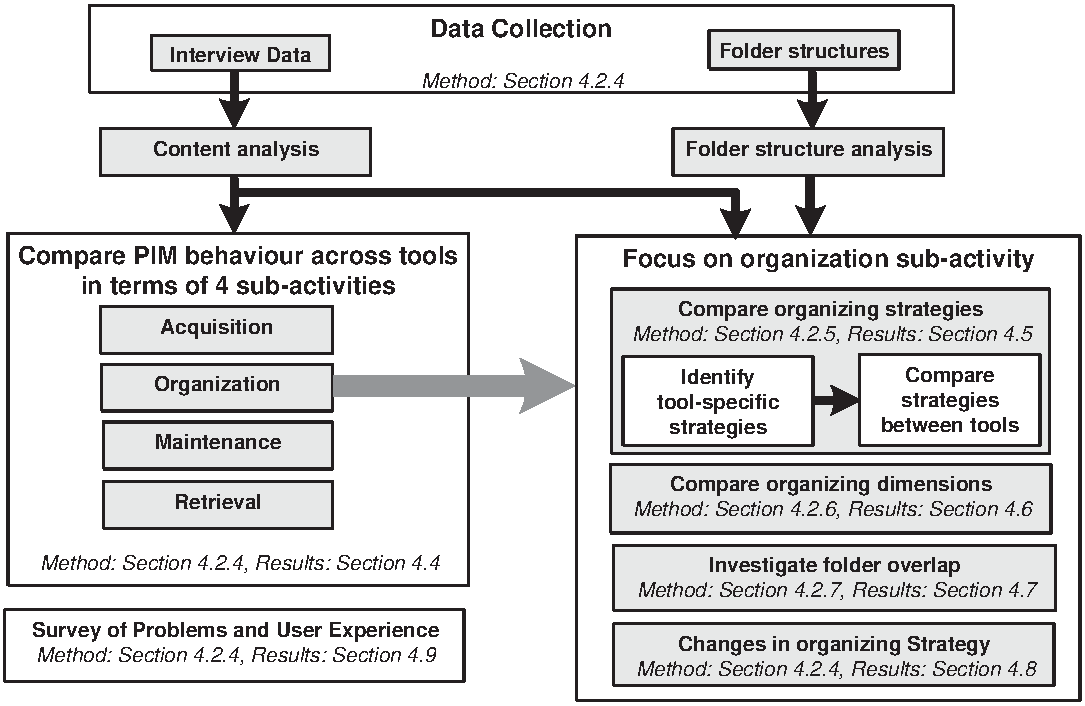
\includegraphics[height=10cm]{pictures/exp-study/analysis-structure.pdf}
		% \includegraphics[height=2in, width=.9 \textwidth]{pictures/exp-study-Overlaps.pdf}
	\end{center}
	\caption{Stages of data analysis}
	\label{fig:exp-study:analysis-structure}
\end{figure}



%%%%%%%%%%%%%%%%%%%%%%%%%%%%%%%%%%%%%%%%%%%%%%%%%%%%%%%%%%%%%%%%%%%%%%%%%%%%%%%%%%%%%%%%%%%%%%%%
%%%%%%%%%%%%%%%%%%%%%%%%%%%%%%%%%%%%%%%%%%%%%%%%%%%%%%%%%%%%%%%%%%%%%%%%%%%%%%%%%%%%%%%%%%%%%%%%
%%%%%%%%%%%%%%%%%%%%%%%%%%%%%%%%%%%%%%%%%%%%%%%%%%%%%%%%%%%%%%%%%%%%%%%%%%%%%%%%%%%%%%%%%%%%%%%%
%%%%%%%%%%%%%%%%%%%%%%%%%%%%%%%%%%%%%%%%%%%%%%%%%%%%%%%%%%%%%%%%%%%%%%%%%%%%%%%%%%%%%%%%%%%%%%%%

%%%%%%%%%%%%%%%%%%%%%%%%%%%%%
\subsection{Choice of Methodology}
\label{exp-study:method-choice}
% SECTION NOTES
% Inspired by the ethnographic method
% Interest: natural setting, investigate/explain phenomena in situ
% Can this be made more convincing?
% Wording: supporters of X claim
%%%%%%%%%%%%%%%%%%%%%%%%%%%%%%
A semi-structured interview methodology was selected, in which a core framework of questions forms the basis for the interviews. In addition, when time permits, the researcher can pursue diversions to related topics as they arise, giving the flexibility to elicit feedback on unexpected, yet relevant issues. This choice is justified for the following reasons. A key aim of the study was to investigate real-world PIM behaviour in a natural setting.  Semi-structured interviews are a standard HCI research methodology for investigating complex computer-based activities~\citep{Robson:01}.  Additionally, semi-structured interviews have been successfully employed in a number of previous studies of PIM, e.g. ~\citep{Whittaker-email:96}.  
 % The interview framework employed in this study is presented in \textbf{Section~\ref{exp-study:interview-process}}.
% Interview flexibility in this manner has proved to be successful in eliciting feedback on unexpected, yet relevant issues in HCI.

%%%%%%%%%%%%%%%%%%%%%%%%%%%%%%%%%%%%%%%%%%%%%%%%%%%%%%%%%%%%%%%%%%%%%%%%%%%%%%%%%%%%%%%%%%%%%%%%
%%%%%%%%%%%%%%%%%%%%%%%%%%%%%%%%%%%%%%%%%%%%%%%%%%%%%%%%%%%%%%%%%%%%%%%%%%%%%%%%%%%%%%%%%%%%%%%%
%%%%%%%%%%%%%%%%%%%%%%%%%%%%%%%%%%%%%%%%%%%%%%%%%%%%%%%%%%%%%%%%%%%%%%%%%%%%%%%%%%%%%%%%%%%%%%%%
%%%%%%%%%%%%%%%%%%%%%%%%%%%%%%%%%%%%%%%%%%%%%%%%%%%%%%%%%%%%%%%%%%%%%%%%%%%%%%%%%%%%%%%%%%%%%%%%

%%%%%%%%%%%%%%%%%%%%%%%%%%%%%%%%
\subsection{Participants}
\label{exp-study:user-selection}
%%%%%%%%%%%%%%%%%%%%%%%%%%%%%%%%
Twenty-five participants took part in the study.  An overview of their details is presented in \textbf{Table~\ref{table:exp-study:user_summary}}.  All participants had at least 5 years of general computing experience, and had used their current operating system for at least one year (19 used MS-Windows, 4 used MacOS, and 2 used Linux).  Of the 25 participants, 7 were female, and 18 were male.  The average age was 37 (ranging from 21 to 60).  The majority (23) were recruited from the academic establishments where the author was pursuing his research programme.
% from the universities where the author carried out his research or visited during his research (Imperial College London, University College London, Waikato University in New Zealand, and the University of Colorado at Boulder, USA).
Roles included researchers (12), students (10), and support staff (1). The final 2 were non-academic: one was a manager for a telecommunications company, and one was unemployed. Participants did not receive any incentive to take part, financial or otherwise. 

%%%%%%%%%%%%%%%%%%%%%%%%%%%%%%%%%%%%%%%%%%%%%%%%%%%%%%%
% TABLE: exploratory study participants
%%%%%%%%%%%%%%%%%%%%%%%%%%%%%%%%%%%%%%%%%%%%%%%%%%%%%%%
\begin{table}[hbt]
\begin{center}
\begin{footnotesize}
\setlength{\extrarowheight}{2pt}
%\begin{tabular}{|p{2.5cm}|p{3.5cm}|p{3.5cm}|p{3.5cm}|}
%	& {\bf Document File} & {\bf Email} &  {\bf Web} \\
% Table generated by Excel2LaTeX from sheet 'EXPLORATORY STUDY PARTICIPANTS'
\begin{tabular}{|c|c|c|c|c|c|}
\hline
    {\bf Participant} &  {\bf Age} &  {\bf Sex} & {\bf Job Role} & {\bf Location} & {\bf Operating System} \\
\hline
         P1 &      35-40 &          M &   Academic &         UK & Windows 2000 \\
\hline
         P2 &      20-25 &          M &    Student &         UK & Windows 2000 \\
\hline
         P3 &      25-30 &          M &    Student &         UK & Windows 2000 \\
\hline
         P4 &      20-25 &          F &    Student &         UK & Windows 2000 \\
\hline
         P5 &      25-30 &          M &    Student &         UK & Windows 98 \\
\hline
         P6 &        60+ &          M &   Academic &         UK &    MacOS 8 \\
\hline
         P7 &      25-30 &          M &    Student &         UK & Windows NT4 \\
\hline
         P8 &      25-30 &          M &    Student &         UK & Windows NT4 \\
\hline
         P9 &      45-50 &          F &   Academic &         NZ &     Macos8 \\
\hline
        P10 &      45-50 &          M &   Academic &         NZ & Windows NT4 \\
\hline
        P11 &      30-35 &          F &   Academic &         NZ & Windows NT4 \\
\hline
        P12 &      25-30 &          M &   Academic &         NZ &      Linux \\
\hline
        P13 &      50-55 &          M &   Academic &         NZ &    MacOS 9 \\
\hline
        P14 &      35-40 &          M &   Academic &         NZ & Windows 2000 \\
\hline
        P15 &      35-40 &          M &   Academic &         NZ & Windows NT4 \\
\hline
        P16 &      40-45 &          M & Technical Support &         NZ &    MacOS X \\
\hline
        P17 &      30-35 &          F &    Student &         NZ & Windows NT4 \\
\hline
        P18 &      25-30 &          M &    Student &         NZ &      Linux \\
\hline
        P19 &      35-40 &          M &   Academic &         NZ & Windows 2000 \\
\hline
        P20 &      30-35 &          M &    Student &        USA & Windows 2000 \\
\hline
        P21 &      30-35 &          F &    Student &        USA & Windows 98 \\
\hline
        P22 &      40-45 &          F &   Academic &         UK & Windows 98 \\
\hline
        P23 &      30-35 &          M &   Academic &         UK & Windows XP \\
\hline
        P24 &        60+ &          M & Unemployed &         UK & Windows 98 \\
\hline
        P25 &      40-45 &          F & Manager &         UK & Windows 2000 \\
\hline
\end{tabular}  
\end{footnotesize}
\caption{Participants in the Exploratory Study}
\label{table:exp-study:user_summary}
\end{center}
\end{table}
\normalsize

%%%%%%%%%%%%%%%%%%%%%%%%%%%%%%%%%%%%%%%%%%%%%%%%%%%%%%%%%%%%%%%%%%%
%\subsection{Working with personal information: ethics and privacy}
%\label{exp-study:ethics}
%%%%%%%%%%%%%%%%%%%%%%%%%%%%%%%%%%%%%%%%%%%%%%%%%%%%%%%%%%%%%%%%%%%
People known to the author were intentionally invited to participate due to concerns regarding the privacy issues associated with the researcher invading strangers' personal space. % check this!
It was envisaged that such familiarity would establish a trust basis, leading to the ability to raise concerns that may arise at any time.  Participants' comments (see \textbf{Section~\ref{exp-study:results-overview}}) suggest this was a valid consideration. 

%%%%%%%%%%%%%%%%%%%%%%%%%%%%%%%%%%%%%%%%%%%%%%%%%%%
% Limitations in terms of statistical significance
%%%%%%%%%%%%%%%%%%%%%%%%%%%%%%%%%%%%%%%%%%%%%%%%%%%
It is acknowledged that the study participants are not a representative sample of the general population of users, and are thus not statistically significant.  However, it is argued that the set of participants matches the purposes of the study well: to establish a comprehensive picture of users' PIM practices.   The results should be interpreted as suggestive (i.e. directed at forming the basis for future research) rather than as providing conclusive findings.
% Note that all the participants were known to the researcher before their participation in the study.  This user sample raises a key methodological point: it may be argued that the selection of participants who were familiar with the researcher may cause experimental bias.
% The selection of users is defended as follows.

%%%%%%%%%%%%%%%%%%%%%%%%%%%%%%%%%%%%%%%%%%%%%%%%%%%%%%%%%%%%%%%%%%%%%%%%%%%%%%%%%%%%%%%%%%%%%%%%
%%%%%%%%%%%%%%%%%%%%%%%%%%%%%%%%%%%%%%%%%%%%%%%%%%%%%%%%%%%%%%%%%%%%%%%%%%%%%%%%%%%%%%%%%%%%%%%%
%%%%%%%%%%%%%%%%%%%%%%%%%%%%%%%%%%%%%%%%%%%%%%%%%%%%%%%%%%%%%%%%%%%%%%%%%%%%%%%%%%%%%%%%%%%%%%%%
%%%%%%%%%%%%%%%%%%%%%%%%%%%%%%%%%%%%%%%%%%%%%%%%%%%%%%%%%%%%%%%%%%%%%%%%%%%%%%%%%%%%%%%%%%%%%%%%

% \newpage
%%%%%%%%%%%%%%%%%%%%%%%%%%%%%%%%
\subsection{Interview Process}
\label{exp-study:interview-process}
%%%%%%%%%%%%%%%%%%%%%%%%%%%%%%%%
% The core framework of each semi-structured interview was as follows.
% Wording: structured field notes sheet
%%%%%%%%%%%%%%%%%%%%%%%%%%%%%%%%
This section provides an overview of the interview format. Complete experimental materials are included in \textbf{Appendix~\ref{chap:appendices-exploratory-study-material}}.

Each interview lasted about 90 minutes, and was carried out in the usual workplace of the interviewee where it was possible to view the participant's activity in context.

%%%%%%%%%%%%%%%%%%%%%%%%%%%%%%%%%
% PRIVACY - BEFORE
%%%%%%%%%%%%%%%%%%%%%%%%%%%%%%%%%
Due to the highly personal nature of PIM, a number of privacy-related precautions were employed.  People frequently feel a sense of guilt towards a messy workspace, whether physical~\citep{tm:83} or electronic~\citep{Bellotti:00}.  % A view held by many people is that a ``tidy'' workspace, where all items are filed away, is superior to a ``messy'' workspace (CITE). However this popular belief has been debated in the literature~\citep{Whittaker-paper:01}.}.
Therefore a primary concern in the study was to not cause the participants to feel uncomfortable. 
The participants were made aware of the nature of the study in advance so that they could take steps to hide anything that they did not want the researcher to see (e.g. confidential information, medical reports, love letters!). However, the participants were asked not to change their collections in any other way before the interview (e.g. tidying their inbox).  This proved to be judicious, e.g. P25: \textit{``So you know what I do now - I would have tidied it up if you'd let me''}. 

%%%%%%%%%%%%%%%%%%%%%%%%%%%%%%%%%
% PRIVACY - START
%%%%%%%%%%%%%%%%%%%%%%%%%%%%%%%%%
Before each interview, the researcher stated that the user's personal approach to managing information was not being evaluated in any way, and all participants signed a release form acknowledging that the data would be anonymised before analysis and publication.  % Participants were reminded that the study was not intended to be a critique of how they organized their workspace.  
Next, basic demographic information was collected (summarized in \textbf{Table~\ref{table:exp-study:user_summary}}), and participants were asked about the main production activities which drove their computer usage. A screenshot of each participant's desktop was also captured.


%%%%%%%%%%%%%%%%%%%%%%%%%%%%%%%%%%%%%%%%%%%%%%%%%%%%%%%%%%%%%%%%%%%%%%%%%%%%%%%%%%%%%%%
% \subsubsection{Guided tour of the document file, email and web bookmarks collections}
%%%%%%%%%%%%%%%%%%%%%%%%%%%%%%%%%%%%%%%%%%%%%%%%%%%%%%%%%%%%%%%%%%%%%%%%%%%%%%%%%%%%%%%

Interviews were centred on guided tours of the files, email and bookmarks that they collected on their main work computer.

The three collections were defined as follows:

\begin{itemize}

%%%%%%%%%%%%%%%%%%%%%%%%%%%%%%%%%%%%%%%%%%
% Definition of file collection
%%%%%%%%%%%%%%%%%%%%%%%%%%%%%%%%%%%%%%%%%%
\item The \textit{document file collection} was defined as the principal area of the file system used by an individual to manage their personal document files. For the purposes of the study, document files were defined as those files containing content such as text, image and music files -- as opposed to executable applications. Since files are often distributed across multiple locations in the file system, participants were asked to identify their primary collection of personal files. Operating systems typically provide a default area for this purpose, such as ``My Documents'' under MS-Windows, or the ``home directory'' under UNIX.  Areas of the file collection that contained source code, simulation data, saved web pages, temporary files and internet downloads were omitted from the interview to save time.  In these cases, only the root folder of each sub-structure was surveyed.  So for example, if a file folder, \texttt{Downloads}, contained a set of sub-folders for downloaded programs, only the top folder was considered in the study.  % Hierarchies often contained extensive sub-structures for source code, simulation data, backups and temporary files. Only the root folder of such sub-structures was included. So for example, if a file folder sub-tree, \texttt{simproj/set3/monday/run2}, contained simulation data, only the top folder \texttt{simproj} was included.


%%%%%%%%%%%%%%%%%%%%%%%%%%%%%%%%%%%%%%%%%%
% Definition of email collection
%%%%%%%%%%%%%%%%%%%%%%%%%%%%%%%%%%%%%%%%%%
\item The \textit{email collection} was defined as the collection of electronic messages stored in the participant's main email tool.  If the participant employed multiple email tools (e.g. MS-Outlook on the desktop, and web-based email such as Hotmail), they were asked to nominate their primary collection.

%%%%%%%%%%%%%%%%%%%%%%%%%%%%%%%%%%%%%%%%%%
% Definition of bookmarks collection
%%%%%%%%%%%%%%%%%%%%%%%%%%%%%%%%%%%%%%%%%%
\item The \textit{web bookmark collection} was defined as the set of ``links'' or ``Favorites'' stored by a participant in their main web browser.
% SEE BELOW: why certain areas of the hierarchy omitted from the interview

\end{itemize}

The use of desktop icons to manage files, email, or bookmarks was also covered.  Icons were considered to be an adjunct to the respective collection.  

At the start of each guided tour, a snapshot was recorded of any folders developed by the participant.  Participants were asked to go through the folders one by one, and talk about their usage. Notes were made of folders that were mentioned as being no longer in use (e.g. failed or duplicate folders).  Participants were also asked about the function of any items that were not filed in folders (i.e. those items at the root-level of the collection, or those managed on the desktop). 

%%%%%%%%%%%%%%%%%%%%%%%%%%%%%%%%%
% PRIVACY - DURING
%%%%%%%%%%%%%%%%%%%%%%%%%%%%%%%%%
Wherever possible during the study, additional procedural steps were taken to avoid privacy infringements. For instance the exposure of the content of specific items of information was avoided wherever possible. One simple yet effective technique was to maximize the folder-view window, thus obscuring the content of specific items.
% Participants were able to do this either before or during the guided tours of their files, email and bookmarks.

During the guided tour participants were asked about their PIM practices within each collection. In order to cover the various aspects of PIM, the interview structure was based on the four point conceptual framework outlined in \textbf{Chapter~\ref{chapter:bg}}: \textit{acquisition} of items, \textit{organization} of those items, \textit{maintenance} of the collection, and \textit{retrieval} of items from the collection.  Participants were also asked about any problems they encountered in each PIM-tool.  Note that due to time limitations, interviews sometimes failed to cover all the above aspects. % EXPAND ME
% Note: that guided tours were not always complete due to lack of time on the part of the interviewer


%%%%%%%%%%%%%%%%%%%%%%%%%%%%%%%%%%%%%%%%%%%%%%%%%%%%%%%%
% Need to add? consideration of each tool separately
%%%%%%%%%%%%%%%%%%%%%%%%%%%%%%%%%%%%%%%%%%%%%%%%%%%%%%%%
% Note that each collection was covered separately. Any references made by the participant in the context of one collection to the other collections were noted (for instance the mention of files managed as attachments within email messages). Participants were asked to comment about the presence of similar folders in the different collections}.

%%%%%%%%%%%%%%%%%%%%%%%%%%%%%%%%%%%%%%%%%%%%%%%%%%%%%%%%%		
% \item \textbf{Overview of the rest of the workspace}
%%%%%%%%%%%%%%%%%%%%%%%%%%%%%%%%%%%%%%%%%%%%%%%%%%%%%%%%%
If time allowed, other collections of personal information were surveyed including those managed in the primary digital workspace (e.g. contacts), on mobile devices (e.g. PDA devices), and in the physical workspace (e.g. piles of documents).
% Although this framework defined the core of each interview, when time allowed diversions to related topics were permitted (e.g. other PIM tools and digital devices).







%%%%%%%%%%%%%%%%%%%%%%%%%%%%%%%%%%%%%%%%%%%%%%%%%%%%%%%%%%%%%%%%%%%%%%%%%%%%%%%%%%%%%%%%%%%%%%%%
%%%%%%%%%%%%%%%%%%%%%%%%%%%%%%%%%%%%%%%%%%%%%%%%%%%%%%%%%%%%%%%%%%%%%%%%%%%%%%%%%%%%%%%%%%%%%%%%
%%%%%%%%%%%%%%%%%%%%%%%%%%%%%%%%%%%%%%%%%%%%%%%%%%%%%%%%%%%%%%%%%%%%%%%%%%%%%%%%%%%%%%%%%%%%%%%%
%%%%%%%%%%%%%%%%%%%%%%%%%%%%%%%%%%%%%%%%%%%%%%%%%%%%%%%%%%%%%%%%%%%%%%%%%%%%%%%%%%%%%%%%%%%%%%%%

%%%%%%%%%%%%%%%%%%%%%%%%%%%%%%%%%%%%%%%%%
% METHOD 1
\subsection{Data Collection and Analysis}
\label{exp-study:data-analysis}
%%%%%%%%%%%%%%%%%%%%%%%%%%%%%%%%%%%%%%%%%

In order to build up a rich picture of participants' PIM practices, both subjective and objective data were collected .  User comments were captured as notes taken during the interview, and annotated with observations made by the researcher. A sample of the collected data is shown in \textbf{Appendix~\ref{chap:appendices--study-data}} on page~\pageref{chap:appendices--study-data:exp-study}.
% i.e. no transcriptions
Objective data was captured in the form of graphical snapshots of the desktop, and of any folder structures developed in each collection.  The author also recorded the number of unfiled items in each collection (items located in the root folder or on the desktop).

% The rest of this section surveys the data analysis that was performed: (1) content analysis of the interview notes, and (2) analysis of the folder structures.

%%%%%%%%%%%%%%%%%%%%%%%%%%%%%%%%%%%%%%%%%%%%%%%%%%%
\subsubsection{Content Analysis of Interview Notes}
%%%%%%%%%%%%%%%%%%%%%%%%%%%%%%%%%%%%%%%%%%%%%%%%%%%
% If required, follow-up meetings were arranged to clarify particular points that were not clear from the data.
% Also nature of items, of the collection in general.}
% changes in PIM strategy.
% integration between the three collections.
%%%%%%%%%%%%%%%%%%%%
% Old Stuff on WTBU
%%%%%%%%%%%%%%%%%%%%
% This qualitative data was used to characterise how participants managed each type of particular information and is reported in \textbf{Section~\ref{exp-study:Results1-WTBU}}.
% \item Content analysis of interview notes in terms of Barreau's conceptual framework.
Content analysis was performed on the interview data to extract key themes relating to PIM.
The content analysis consisted of several passes through the interview notes. A first pass lead to the development of a coding scheme listing key themes such as strategies, problems, design suggestions, and changes in strategy over time. Comments were also extracted relating to integration between PIM-tools. % both existing integration and needs for improved integration
During subsequent passes, the coding scheme was used to mark up the data, and extended with any further issues that emerged.  Finally, the themes were clustered using the four PIM sub-activities from
\textbf{Chapter~\ref{chapter:bg}} (acquisition, organization, maintenance, and retrieval), and arranged in terms of frequency and importance. % Relevant quotes were extracted to illustrate user behaviour.

The comparison of typical behaviour between the tools in terms of the four PIM sub-activities is reported in \textbf{Section~\ref{exp-study:Results-comparison}}\footnote{Note that the objective data (in the form of the folder hierarchies) was focused on one PIM sub-activity: organizing.  The non-longitudinal nature of the study meant that information regarding the other PIM sub-activities (acquisition, maintenance and retrieval) was as reported by each user and subjective in nature.}.  Changes in organizing strategy, and findings related to PIM problems are reported in \textbf{Sections~\ref{exp-study:comparison-changes}} and \textbf{\ref{exp-study:comparison-problems}} respectively.

\textbf{Section~\ref{exp-study:cross-tool-profiling}} describes how the qualitative data also contributed towards the classification of participants' organizing strategies with respect to files, email and bookmarks.

%%%%%%%%%%%%%%%%%%%%%%%%%%%%%%%%%%%%%%%%%%%%%%%%%%%
\subsubsection{Analysis of Folder Hierarchies}
%%%%%%%%%%%%%%%%%%%%%%%%%%%%%%%%%%%%%%%%%%%%%%%%%%%
% The analysis of folder structures consisted of three steps.

The folder hierarchies were transcribed, and marked up with participant's comments as to the function and usage of specific folders. % NB: this is a great argument for longitudinal studies
% Data analysis consisted of the following stages, including two novel techniques developed by the author to analyse and compare the folder hierarchies:
%%%%%%%%%%%%%%%%%%%%%%%%%%
% ANALYSIS1: BASIC STATS
%%%%%%%%%%%%%%%%%%%%%%%%%%
% NOT CAPTURED CONSISTENTLY: number of failed/active folders,
% THINK: need to explain hierarchy depth? (e.g. in email)
Then, basic statistics were extracted from each hierarchy including number of folders, number of unfiled items, and hierarchy depth. These are reported under the organizing PIM sub-activity in \textbf{Section~\ref{exp-study:comparison-organization}}.  As noted above, any file folder sub-structures containing source code, simulation data, or downloaded programs were omitted.

The folder structures were then analysed using two novel techniques, developed by the author.
%%%%%%%%%%%%%%%%%%%%%%%%%%%%%%%%%%%%%%%%
% ANALYSIS 2: ORGANISATIONAL DIMENSIONS
%%%%%%%%%%%%%%%%%%%%%%%%%%%%%%%%%%%%%%%%
\textbf{Section~\ref{exp-study:folder-analysis-orgdim}} reports the analysis of the \textit{organizational dimensions} used to name folders (e.g. \textit{project}, \textit{contact}, \textit{place}). 
%%%%%%%%%%%%%%%%%%%%%%%%%%%%%%%
% ANALYSIS 3: FOLDER OVERLAP
%%%%%%%%%%%%%%%%%%%%%%%%%%%%%%%
\textbf{Section~\ref{exp-study:analysis-folder-overlap}} reports the investigation of \textit{folder overlap}.

%%%%%%%%%%%%%%%%%%%%%%%%%%%%%%%%%%%%%%%%%%%%%%%%%%%%%%%%%%%%%%%%%%%%%%%%%%%%%%%%%%%%%%%%%%%%%%%%
%%%%%%%%%%%%%%%%%%%%%%%%%%%%%%%%%%%%%%%%%%%%%%%%%%%%%%%%%%%%%%%%%%%%%%%%%%%%%%%%%%%%%%%%%%%%%%%%
%%%%%%%%%%%%%%%%%%%%%%%%%%%%%%%%%%%%%%%%%%%%%%%%%%%%%%%%%%%%%%%%%%%%%%%%%%%%%%%%%%%%%%%%%%%%%%%%
%%%%%%%%%%%%%%%%%%%%%%%%%%%%%%%%%%%%%%%%%%%%%%%%%%%%%%%%%%%%%%%%%%%%%%%%%%%%%%%%%%%%%%%%%%%%%%%%


%%%%%%%%%%%%%%%%%%%%%%%%%%%%%%%%%
% METHOD 2
%\subsection{Method: Comparing PIM Behaviour}
%\label{exp-study:behaviour-comparison}
%%%%%%%%%%%%%%%%%%%%%%%%%%%%%%%%%
%%%%%%%%%%%%%%%%%%%%%%%%%%%%%%%%%
%%%%%%%%%%%%%%%%%%%%%%%%%%%%%%%%%
% CONTENT1: Comparing the nature of PIM
%%%%%%%%%%%%%%%%%%%%%%%%%%%%%%%%%
% For each PIM sub-activity, typical behaviour was compared between the three PIM-tools, to investigate whether similar strategies were used to manage different types of information. Based on these tool-specific characterizations, the management of each type of information was compared at an abstract \textit{cross-user} level (generalized across all participants) to answer the question: \textit{Across participants in general, how does the management of the three types of information compare?}. These results are reported in \textbf{Section~\ref{exp-study:Results-comparison}}.


%%%%%%%%%%%%%%%%%%%%%%%%%%%%%%%%%%%%%%%%%%%%%%%%%%%%%%%%%%%%%%%%%%%%%%%%%%%%%%%%%%%%%%%%%%%%%%%%
%%%%%%%%%%%%%%%%%%%%%%%%%%%%%%%%%%%%%%%%%%%%%%%%%%%%%%%%%%%%%%%%%%%%%%%%%%%%%%%%%%%%%%%%%%%%%%%%
%%%%%%%%%%%%%%%%%%%%%%%%%%%%%%%%%%%%%%%%%%%%%%%%%%%%%%%%%%%%%%%%%%%%%%%%%%%%%%%%%%%%%%%%%%%%%%%%
%%%%%%%%%%%%%%%%%%%%%%%%%%%%%%%%%%%%%%%%%%%%%%%%%%%%%%%%%%%%%%%%%%%%%%%%%%%%%%%%%%%%%%%%%%%%%%%%

% \newpage
%%%%%%%%%%%%%%%%%%%%%%%%%%%%%%%%%
%%%%%%%%%%%%%%%%%%%%%%%%%%%%%%%%%
% METHOD 4
\newpage
\subsection{Method: Comparing Organizing Strategies}
\label{exp-study:cross-tool-profiling}
%%%%%%%%%%%%%%%%%%%%%%%%%%%%%%%%%
%%%%%%%%%%%%%%%%%%%%%%%%%%%%%%%%%
% \textbf{Section~\ref{exp-study:cross-tool-profiling}} details the cross-tool profiling of individuals' filing behaviour.

The analysis of organizing strategies consisted of two stages:
\begin{enumerate}
	\item Classifying each participants' strategies in each collection in turn.
	\item Comparing each participants' strategies between their three collections.
\end{enumerate}

%%%%%%%%%%%%%%%%%%%%%%%%%%%%%
% TOOL-SPECIFIC PROFILING
%%%%%%%%%%%%%%%%%%%%%%%%%%%%%
Firstly, organizing strategies were characterised for each participant in the 3 PIM-tools.
% \textbf{Section~\ref{exp-study:data-analysis}} describes the content analysis performed to identify the management strategies employed by participants in each of the three tools.
In each tool a classification scheme was devised by the author to categorize the participants based on their reported management strategies.  Previous classifications of organizing strategies that have been proposed in email~\citep{Whittaker-email:96} and for bookmarks~\citep{da:98} were used as a starting point in those two contexts.  Classifications were based on a combination of objective data (e.g. folder counts) and participants' comments.  Qualitative data was employed as it was not always straightforward to distinguish current strategies based on objective data alone.  For instance, a large folder count may suggest a user who files most information.  However, in many cases folders were abandoned.  Qualitative data was useful in indicating whther this was the case.
The three tool-specific classification schemes (for files, email, and bookmarks) are reported in \textbf{Sections~\ref{exp-study:Results-org-strategies-files}}, \textbf{\ref{exp-study:Results-org-strategies-email}}, and \textbf{\ref{exp-study:Results-org-strategies-bookmarks}}.

%%%%%%%%%%%%%%%%%%%%%%%%%%%%%%%%%
% CROSS-TOOL PROFILING
%%%%%%%%%%%%%%%%%%%%%%%%%%%%%%%%%
% Based on this within-tool analysis, the nature of PIM is compared between the three tools.
% The data relating to each PIM-tool was collated together across all participants. Then for each PIM-tool, the most common PIM strategies were identified, and a classification of user behaviour proposed.
% This analysis was aimed at characterizing the most common PIM practices -- observed across all participants -- regarding each type of information (technological format) in turn: files, email, and bookmarks. 
% WT/BU PERSPECTIVE: This analytical perspective is equivalent to that employed in previous tool-specific studies (see \textit{\textbf{Chapter~\ref{chapter:review}}}), and can be considered as an attempt to answer the question: \textit{Can PIM practices within particular collections be characterized across all study participants?} 
% By comparing the management of a particular type of information across multiple users, it is possible to classify the users in terms of the strategies used to manage files, email and bookmarks in turn.
% A particular focus was taken on the sub-activity of organization, and for each tool a classification of participants' reported filing behaviour is presented. 
The comparison stage was carried out to investigate whether individual participants employed consistent organizing strategies across their collections. The driving interest was to investigate whether participants who were relatively organized in files were also relatively organized in the other tools, and vice versa.  For each participant, a cross-tool profile was produced by collating the three tool-specific strategies from the previous stage.  Since the cross-tool profiling employed the tool-specific classifications, the method is discussed in detail in \textbf{Section~\ref{exp-study:Results-cross-tool-profiling}}, along with the results.
% This was performed to investigate whether individual participants employed consistent strategies across their collections (in terms of whether they reported devoting significant effort to organizing multiple types of information). 

%WE compared each participant's organizing strategies between the three collections to investigate the consistency of their organizing/filing behaviour.
% This approach goes beyond previous work by attempting to build up a \textit{cross-tool} profile of user behaviour.
Previous empirical studies have focused on individual usage of specific tools such as email. In contrast, this analysis attempts to go beyond previous work by constructing a cross-tool profile of behaviour to investigate how organizing practices vary between the collections for individual users.  % The \textit{cross-tool profiling} technique is described in more detail in \textbf{Section~\ref{exp-study:cross-tool-profiling}}.
% The previous analysis compared generalized behaviour between the tools.
% Rather than generalizing across all participants as in the previous stage, the aim was to focus on individuals. This analysis was directed at exploring similarities and differences between the three collections to investigate potential compatibility for integration and/or unification.





%%%%%%%%%%%%%%%%%%%%%%%%%%%%%%%%%%%%%%%%%%%%%%%%%%%%%%%%%%%%%%%%%%%%%%%%%%%%%%%%%%%%%%%%%%%%%%%%
%%%%%%%%%%%%%%%%%%%%%%%%%%%%%%%%%%%%%%%%%%%%%%%%%%%%%%%%%%%%%%%%%%%%%%%%%%%%%%%%%%%%%%%%%%%%%%%%
%%%%%%%%%%%%%%%%%%%%%%%%%%%%%%%%%%%%%%%%%%%%%%%%%%%%%%%%%%%%%%%%%%%%%%%%%%%%%%%%%%%%%%%%%%%%%%%%
%%%%%%%%%%%%%%%%%%%%%%%%%%%%%%%%%%%%%%%%%%%%%%%%%%%%%%%%%%%%%%%%%%%%%%%%%%%%%%%%%%%%%%%%%%%%%%%%

%%%%%%%%%%%%%%%%%%%%%%%%%%%%%%%%%
%%%%%%%%%%%%%%%%%%%%%%%%%%%%%%%%%
% METHOD 2
\subsection{Method: Analysis of Organizational Dimensions}
\label{exp-study:folder-analysis-orgdim}
%%%%%%%%%%%%%%%%%%%%%%%%%%%%%%%%%
%%%%%%%%%%%%%%%%%%%%%%%%%%%%%%%%%
% employed in the \textit{within-tool/between-users analysis} detailed below
% These results are reported along with the qualitative findings relating to folder organization in
% %  For example the email folder ``Eric'' is based on \textit{contact}.  This technique was used to compare the types of folders created in the three collections of personal information. The motivation and execution of this technique is discussed in more detail in .  % Results are reported in \textbf{Section~\ref{exp-study:Results-org-dims}}.
% including the most common organizational dimensions used to classify each type of information. 
%%%%%%%%
% INTRO
%%%%%%%%
% The technique was used to characterize the types of folders developed within each collection of personal information. 
% The term \textit{organizational dimension} is used in this thesis to mean type of concept on which a folder name is based.  
This section presents a technique developed by the author to analyse the \textit{organizational dimensions} present in a folder structure -- \textit{the types of concept on which folder names are based (e.g. project, place, contact)}.


% Firstly, the rationale behind the technique is discussed, followed by detail of its execution.
%%%%%%%%%%%%%%%%%%%%%%%%%%%%%%%%%%%%
\subsubsection{Motivation and Aim}
%%%%%%%%%%%%%%%%%%%%%%%%%%%%%%%%%%%%
%% ADD other terms for organizational dimension in the literature.
%% Common examples noted in the literature include events (e.g. ``Jill's wedding''), roles (e.g. ``Teaching'') and people (e.g. ``Brian'') (\textit{CITE}). 
The development of the technique was motivated on two counts.
Firstly, previous studies have noted the existence of particular types of folders. For instance, \citet{Ducheneaut:01} observed that most email folders were based on \textit{sender}, \textit{organization}, \textit{project}, or \textit{interest}.  They also observed that the relative proportions of folder types varied significantly between users.  Similar \textit{ad hoc} observations of common folder types have been used by designers as the design rationale for PIM-unification systems based on a dominant organizational dimension such as \textit{role}~\citep{Shneiderman:94} or \textit{project}~\citep{Kaptelinin:03}.  However, no systematic analysis of folder types has been performed to date.

Secondly, during the guided tours in this study, many participants referred to various organizational dimensions. % Commonly mentioned folder types included \textit{projects}, \textit{roles} and \textit{interests}.
For example, P22 summarized her file folders as follows: \textit{``They are organized by projects, activities and roles such as `PhD tutor'. Oh, and this is bad, I also have a `Papers' folder where I keep all the papers that I've written, authored or co-authored. And they're broken down by co-author, cos I'm usually a co-writer''}.  In this statement four organizational dimensions are cited: \textit{projects}, \textit{activities}, \textit{roles} and \textit{people}. % Such dimensions can be considered as a description of the types of concept on which folder names are based.

%%%%%%%
% Aims
%%%%%%%
%%%%%%%%%%%%%%%
% Implications
%%%%%%%%%%%%%%%

% As a first step WE were interested in generalizing our analysis of organizational dimensions across users: \textit{Are personal information collections of a particular technological format dominated by particular organizational dimensions? Are different types of information dominated by different sets of organizational dimensions?}
% My \textit{a priori} hypothesis, based on what WE had seen in the data was that users employ a wide variety of organisational dimensions to structure their collections of document files, email and web bookmarks.
The objective of this analysis was two-fold.
\begin{enumerate}
% (1) explore what types of organizational dimension appeared in each tool (\textit{Research question: what types of organizational dimension are meaningful for users when organizing a particular type of information?}), 
\item To characterise the most common organizational dimensions within each PIM-tool. 
% and then (2) (\textit{Research question: How do organizational dimensions vary between tools?}.
% this would indicate that the users require a high level of organisational flexibility. T  
\item To compare PIM-tools in terms of their most common organizational dimensions.
\end{enumerate}

%%%%%%%%%%%%%%%%%%%%%%%%%%%%%%%
% Relate to previous studies
%%%%%%%%%%%%%%%%%%%%%%%%%%%%%%%
%% Avoid repeating the literature review!
%%
%% Points to get in comparing my approach to Barreau etc.'s: In the style of Kwasnik and Barreau, this study is based on the subjects' own resources (\textit{ADD: unlike GD}). 
%
% \textit{Focus on folders-only (plus user description) versus general description of classification behaviour -- talking generally about handling items (not quite true, WE annotated folder lists with user comments). In contrast to all three previous studies, dimensional analysis is based directly on folder names (and the descriptions participants offered of those folder names offered during the guided tour. In the previous studies analysis was based on general descriptions of classificatory behaviour. The more direct approach was chosen because of the larger amount of material to be analysed (in terms of number of users and number of classification schemes compared to the above studies). }
The existence of a dominant dimension across all tools for a particular user may indicate an optimum subordinate dimension for unification.  In contrast, if a user employs a variety of dimensions across different collections, this would represent a possible barrier against unification, and suggest that basing organizational support on a single subordinate dimension such as \textit{role}~\citep{Shneiderman:94} would overly constrain that user.

This approach can be contrasted with earlier investigations of classification behaviour in physical document~\citep{kwas:91}, digital file~\citep{barreau:95}, and web bookmark collections~\citep{gd:01}. In this body of previous work, analysis was centred on participants' descriptions of their classificatory behaviour.  Here, analysis focused on folder names and the descriptions of those folder names offered by participants during the guided tour.  In addition, this study compares between three different PIM-tools.
% In her study of physical PIM, Kwasnik~\citep{kwas:91} identified a range of factors that influenced the classification included those based on attributes of the document content such as author and topic, and those based on document context such as importance and activity. A similar technique has been employed more recently in the electronic domain in studies of applied similar methods to the electronic domain, in their studies of files~\citep{barreau:95} and web bookmarks~\citep{gd:01}. 



%%%%%%%%%%%%%%%%%%%%%%
\subsubsection{Method}
%%%%%%%%%%%%%%%%%%%%%%

A coding scheme was developed representing the various organizational dimensions manifested in folder names.  The scheme was initially seeded based on proposed PIM-unification technologies that have been based on a subordinate organizational dimension: \textit{role} (defined as long-term user activity)~\citep{Shneiderman:94}, \textit{project} (defined as short-term user activity)~\citep{Kaptelinin:03}, \textit{time}~\citep{Gelernter:96a} and \textit{contact}~\citep{Whittaker-contactmap:02b}.
An iterative coding process was then applied to the folder structures. Each file, email and bookmark folder was coded with the most relevant organizational dimension. At the same time, the coding scheme was extended to include organizational dimensions that were not represented.  Eventually a list of seventeen organizational dimensions was finalized that classified all the folders generated by the participants. 
% CHECK NUMBER fourteen fourteen
% CHECK NUMBER fourteen fourteen
% CHECK NUMBER fourteen fourteen
% CHECK NUMBER fourteen fourteen% CHECK NUMBER fourteen fourteen% CHECK NUMBER fourteen fourteen
% CHECK NUMBER fourteen fourteen
% CHECK NUMBER fourteen fourteen% CHECK NUMBER fourteen fourteen
% CHECK NUMBER fourteen fourteen
The final coding scheme is shown in \textbf{Table~\ref{table:exp-study:dimensions}}, along with some example folders of each type. % Folders were also coded with the secondary dimensions based on comments made during the interviews: coding-related folder (\#), shared folder (+), failed (empty) folder (-), and duplicate folder (\%).

% %%%%%%%%%%%%%%%%%%%%%%%%%%%%%
% TABLE - CODING SCHEME FOR ORGDIMS
% %%%%%%%%%%%%%%%%%%%%%%%%%%%%%
\begin{table}[hbt]
\begin{center}
\begin{footnotesize}
\setlength{\extrarowheight}{2pt}
\begin{tabular}{|c|c|p{3cm}|p{3cm}|}
\hline
{\bf Organisational dimension} & {\bf Code} & {\bf Description} & {\bf Examples} \\
\hline
Project &          P & Short-term production activity & ``Experiment'', ``Agent code'' \\
\hline
Role &          R & Long-term production activity & ``Teaching'', ``Personal'' \\
\hline
Topic / Interest &          I & Subject matter of item & ``Banking'', ``Science Fiction'' \\
\hline
Contact &          C & individual or organisation & ``Rick'', ``ACM'' \\
\hline
Time &          T &  & ``February'', ``tomorrow'' \\
\hline
General &          G &  & ``Stuff'', ``misc'' \\
\hline
Format &          F & Technological format of item & ``Excel sheets'', ``Word document'' \\
\hline
Class of document &          d & Type/class of item & ``Letters'', ``References'' \\
\hline
Workflow &          W &            &  ``Pending'' \\
\hline
Event &          E & Related to a particular occasion such as a meeting or conference &  ``CHI2000'' \\
\hline
Mailing list &          L &            & ``linux-users'' \\
\hline
Version control &          V &            & ``version1'', ``old'' \\
\hline
 Temporary &          t &            & ``temp'', ``tmp'' \\
\hline
Application &          A & Generated automatically by software & ``From ICQ'' \\
\hline
Backup &          B  &            & ``backup'', ``archive'' \\
\hline
Use &          U  &            & ``important'' \\
\hline
Geographic location &          G  &            & ``peckham'' \\
\hline
\end{tabular}  
\end{footnotesize}
\caption{Coding scheme of organizational dimensions}
\label{table:exp-study:dimensions}
\end{center}
\end{table}

Each folder was mapped to one dimension only.  \citet{jc:82} observed complex conventions for naming files.  Similarly complex folder-naming schemes were observed here, and in some cases folder labels were made up of several dimensions. For instance, \texttt{Personal-May} is made up of a combination of the \textit{role} and \textit{time} dimensions.  In such cases, only the first dimension was coded against the folder. %% CHECK

Hierarchies often contained extensive sub-structures for source code, simulation data, backups and temporary files. Only the root folder of such sub-structures was included. So for example, consider a file folder sub-structure, \texttt{simproj/set3/monday/run2}, containing simulation data. In this case, only the top folder \texttt{simproj} was included as a \textit{project} folder.

%%%%%%%%%%%%%%%%%%%%%%%%%%%%%%%%%%%%%%%%%%%
% DIFFICULTIES IN ASSIGNING FOLDER CODES
%%%%%%%%%%%%%%%%%%%%%%%%%%%%%%%%%%%%%%%%%%%
% \textit{Explain why this was not a problem!}.
Folder labels that were ambiguous in some way were confirmed with the subject when possible. Where this was not possible, a subjective coding decision was made by the researcher.  Assigning dimensions involved several challenges:

% However, in some cases, the meaning of particular folders was difficult to interpret. 
\begin{enumerate}

\item \textit{Deciphering abbreviated folder names} -- Some short-hand folder names were difficult to interpret, e.g. participant P24 had many minimal folder names such as \texttt{a2} and \texttt{fjk}.

\item \textit{Non-English folder names} -- Most participants used English to label folders.  However, since participants were drawn from a wide range of nationalities, several other languages were occasionally used to name folders, including Swedish, German, and Portuguese.  In such cases participants were asked for a translation.  % All were asked for translations during interviews where possible. 

\item \textit{Ambiguous folder-to-code mapping} -- In some cases, it was possible to map folder names to multiple codes.  For example, the folder \texttt{jobs} may be interpreted in three ways: (1) as a \textit{document class} (i.e. job adverts), (2) as a \textit{topic}, or (3) as a surname (\textit{contact}).  In the absence of a description from the participant, an estimation was made by the researcher.

% The author attempted to map folders to codes based on the participant's description.

% \item \textit{Multiple folder-to-code mappings} --  % \textbf{CHECK THIS}.

% \textbf{Add examples}.
\end{enumerate}		

%%%%%%%%%%%%%%%%%%%%%%%%%%%%%%
% Collate across all users
%%%%%%%%%%%%%%%%%%%%%%%%%%%%%%
For each PIM-tool, the most common organizational dimensions were identified by collating the coded data across all users.  The results of this analysis are reported in \textbf{Section~\ref{exp-study:Results-org-dims}}. This technique was also used in the subsequent investigation of folder overlap (see \textbf{Section~\ref{exp-study:analysis-folder-overlap}}). % The results of this analysis are reported in \textbf{Section~\ref{exp-study:Results-folder-overlap}}.


%%%%%%%%%%%%%%%%%%%%%%%%%%%%%%%%%%%%%%%%%%%%%%%%%%%%%%%%%%%%%%
% Limitations: only concerned with organizational metadata.
%%%%%%%%%%%%%%%%%%%%%%%%%%%%%%%%%%%%%%%%%%%%%%%%%%%%%%%%%%%%%%
% (\textit{ADD DEFINITION IN PIM-CF}).
%  No attention was paid to any implicit metadata that the users relied on when sorting information (e.g. \textit{subject} or \textit{date received} in email).
Several limitations to this analysis are acknowledged.  Firstly, the analysis is based on explicit structural metadata only -- other forms of organization was not encompassed (e.g. spatial grouping of icons on the desktop).  Secondly, some areas of the folder structures were omitted (e.g. temporary data). Finally, in the cases outlined above, coding may have been non-optimal.  Therefore the results should be taken as indicative only. However, it is argued that these limitations are acceptable considering the exploratory nature of the study.
% this maps well to the aim of the study: to get an overview comparison of how different types of information are managed.



%%%%%%%%%%%%%%%%%%%%%%%%%%%%%%%%%%%%%%%%%%%%%%%%%%%%%%%%%%%%%%%%%%%%%%%%%%%%%%%%%%%%%%%%%%%%%%%%
%%%%%%%%%%%%%%%%%%%%%%%%%%%%%%%%%%%%%%%%%%%%%%%%%%%%%%%%%%%%%%%%%%%%%%%%%%%%%%%%%%%%%%%%%%%%%%%%
%%%%%%%%%%%%%%%%%%%%%%%%%%%%%%%%%%%%%%%%%%%%%%%%%%%%%%%%%%%%%%%%%%%%%%%%%%%%%%%%%%%%%%%%%%%%%%%%
%%%%%%%%%%%%%%%%%%%%%%%%%%%%%%%%%%%%%%%%%%%%%%%%%%%%%%%%%%%%%%%%%%%%%%%%%%%%%%%%%%%%%%%%%%%%%%%%

% \newpage
%%%%%%%%%%%%%%%%%%%%%%%%%%%%%%%%%
%%%%%%%%%%%%%%%%%%%%%%%%%%%%%%%%%
% METHOD 3
\subsection{Method: Analysis of Folder overlap}
\label{exp-study:analysis-folder-overlap}
%%%%%%%%%%%%%%%%%%%%%%%%%%%%%%%%%
%%%%%%%%%%%%%%%%%%%%%%%%%%%%%%%%%

This section describes the second novel technique developed by the author to analyse personal folder structures. The technique is used for assessing the similarity of two collections of personal information in terms of \textit{folder overlap}: the extent to which folders referring to the same activity appear in multiple collections. % CHANGE

%%%%%%%%%%%%%%%%%%%%%%%%%%%%%%%%%%%%
\subsubsection{Motivation and Aim}
%%%%%%%%%%%%%%%%%%%%%%%%%%%%%%%%%%%%
The technique was motivated as follows. Firstly, previous studies have observed overlapping folders.  For example, \citet{Kaptelinin:03} notes that a user may manage and organize multiple types of information when working on a particular project.  He notes that a user working on a software project may author source code documents, receive emails and browse useful websites whilst carrying out the work -- and file them within identical folders in each tool. However, no systematic investigation of folder overlap across a set of users has been carried out.

Additionally, during the guided tours in this study, several participants commented on folders that had appeared in other collections. For a few participants, some folders overlapped between all three collections. For example, P14 had \texttt{Teaching}, \texttt{Research} and \texttt{Personal} folders in his file, email \textit{and} web bookmark hierarchies.  More commonly, there was a partial overlap which varied between the different pairs of collections, e.g. P13: \textit{``The email folders are fairly close to the file system, but with some differences. For example this folder contains correspondence-based information which does not make sense in the file system''}.  



The aim here was to go beyond previous work, and investigate the extent of folder overlap for each participant.  The author was interested in how folder overlap might be used as a measure of the compatibility of different personal classification schemes to be unified.  % Folder overlap may relate to activities that involve the organization of multiple types of information, and thus have the most to gain from increased integration.

%%%%%%%%%%%%%%%%%%%%%%
% MOVE TO RESULTS?
%%%%%%%%%%%%%%%%%%%%%%
% Such activities may have most to benefit from increased integration between PIM tools.  
% It was hypothesised that folder overlap may indicate that the different personal classification schemes tend to converge even when managed separately. 
% In contrast, a low level of folder overlap may indicate a barrier to integration -- that different organizational structures are being used for each type of information.  In addition, some activities may be specific to one collection only (e.g. checking the weather on-line may only involve the management of web bookmarks).  

%%%%%%%%%%%%%%%%%%%%%%%%%
\subsubsection{Method}
%%%%%%%%%%%%%%%%%%%%%%%%%

% This analysis was only carried out for those participants who had developed folders in multiple collections.
 % For users with folders in all three collections, the number of folders that appeared in all three collections was also calculated.
% Each of these participants possessed up to three folder structures: files, email and bookmarks.
For each pair of PIM-tools in which folder structures had been developed, the number of overlapping folders was calculated (see \textbf{Figure~\ref{fig:exp-study:overlaps}}).  For a user with folders in the file, email and bookmark collections, overlaps were calculated for all three hierarchy pairs: \textit{file/email}, \textit{file/web} and \textit{email/web} .

% %%%%%%%%%%%%%%%%%%%%%%%%%%%%%%%%%%%%%%%%%%%%
% FIGURE - THE THREE OVERLAPS
% %%%%%%%%%%%%%%%%%%%%%%%%%%%%%%%%%%%%%%%%%%%%
\begin{figure}[hbtp]
	\begin{center}
		\leavevmode
			\includegraphics{pictures/exp-study/exp-study-Overlaps.pdf}
		% \includegraphics[height=2in, width=.9 \textwidth]{pictures/exp-study-Overlaps.pdf}
	\end{center}
	\caption{Three folder overlaps: file/email, file/bookmark, and email/bookmark}
	\label{fig:exp-study:overlaps}
\end{figure}

A folder was considered to overlap if one of the following three conditions held:

\begin{enumerate}

%%%%%%%%%%%%%%%%%%%%%
% CASE 1: identical
%%%%%%%%%%%%%%%%%%%%%
\item \textit{Identically-named folders in both collections} -- This was the simplest case, e.g. a folder in both the file and email collections called \texttt{Beagle}.

%%%%%%%%%%%%%%%%%%%%%%%%%%%%%%%%%%%%%%%%%
% CASE 2: minor differences were ignored
%%%%%%%%%%%%%%%%%%%%%%%%%%%%%%%%%%%%%%%%%
\item \textit{Folder names that differed slightly} -- In many cases, folder names differ slightly between collections due to spelling mistakes, or variations in \textit{specific phraseology}~\citep{gd:01}.  For example, participant P24 had a \texttt{compiler-course} file folder, and a \texttt{compilers} email folder.  Her comments in the guided tours confirmed that both folders related to the same course that she was teaching.	 % Such minor differences were ignored.
% Minor differences were ignored (e.g. folder names \texttt{CHI2004} and \texttt{chi04} considered identical).

%%%%%%%%%%%%%%%%%%%%%%%%%%%%%%%%%%%%%%%%%%%%%%%%%%%%%%%%%%%%%%%%%%%%%%%%%%%%%%%%%%%%
% CASE 3: different labels relating to the same activity were considered to overlap
%%%%%%%%%%%%%%%%%%%%%%%%%%%%%%%%%%%%%%%%%%%%%%%%%%%%%%%%%%%%%%%%%%%%%%%%%%%%%%%%%%%%
% THINK: how do I map this to organizational dimension?
\item \textit{The use of different folder names to refer to the same activity} -- Occasionally participant's commentaries highlighted cases whereby different folder names related to the same activity.  One example, which applied to three participants, again related to the teaching of a course.  In one tool the respective folder was named after the \textit{course name}, but after the \textit{course codes} in another (e.g. \texttt{compilers} and \texttt{w345}).  User descriptions were taken into account to confirm whether such folders related to the same activity.

\end{enumerate}

%%%%%%%%%%%%%%%%%%%%%%%%%%
% NB: WE ignored depth
%%%%%%%%%%%%%%%%%%%%%%%%%%
Note that folder overlap was calculated based on a flat list of folders. Differences in terms of depth and location were not taken into account.  For example, one participant had a root-level \texttt{Student-projects} folder in email, and a \texttt{Teaching/student-projects} second-level folder in the file collection, which were classed as overlapping.
% Change this example
% Cases such as this were classed as overlapping. 

%%%%%%%%%%%%
% Reporting
%%%%%%%%%%%%
Folder overlap between a pair of collections was presented as a count of overlapping folders, along with the relative percentage of the folders in each collection.  Overlapping folders were then coded in terms of \textit{organizational dimensions} (see \textbf{Section~\ref{exp-study:folder-analysis-orgdim}}). This was carried out to investigate whether overlapping folders tended to be based on a particular organisational dimension.  
%%%%%%%%%%%%%%%%%%%%
% Refer to results
%%%%%%%%%%%%%%%%%%%%
The results from the analysis of folder overlap are presented in \textbf{Section~\ref{exp-study:Results-folder-overlap}}.

%%%%%%%%%%%%
% Problems
%%%%%%%%%%%%
The analysis of folder overlap was time-consuming due to the need to cater for all the above possibilities, particularly when participants had created large numbers of folders.  In a number of cases, participants did not complete the guided tour of all their folders, and the author was required to make some subjective estimations of overlap.  Where possible, these were confirmed with the participant.  However, it is acknowledged that certain false-positives and false-negatives may have crept in.  Despite this limitation, the analysis is offered as a technique to estimate the extent of folder overlap, and thus assess the extent to which user activities involve the organization of multiple types of personal information.

% One example may be folders with the same name referring to different concepts in each tool (e.g. file-folder: ``chess'' referring to the musical, and email-folder: ``chess'' referring to the leisure activity).

%%%%%%%%%%%%%%%%%%%%%%%%%%%%%%%%%%%%%%%%%%%%%%%%%%
% FOR METHOD DETAIL see Results section.
%%%%%%%%%%%%%%%%%%%%%%%%%%%%%%%%%%%%%%%%%%%%%%%%%%



%%%%%%%%%%%%%%%%%%%%%%%%%%%%%%%
% CHAPTER 4: EXPLORATORY STUDY
%%%%%%%%%%%%%%%%%%%%%%%%%%%%%%%
% Overview of results
%%%%%%%%%%%%%%%%%%%%%%%%%%%%%%%%%%%%%%%%%%%%%%%%
%%%%%%%%%%%%%%%%%%%%%%%%%%%%%%%%%%%%%%%%%%%%%%%%
\newpage
%%%%%%%%%%%%%%%%%%%%%%%%%%%%%%%%%%
\section{Initial Observations and Results Overview}
\label{exp-study:results-overview}
% CHECK ORDERING
% SIGNPOSTING
%%%%%%%%%%%%%%%%%%%%%%%%%%%%%%%%%%

All 25 participants actively collected both files and email. 24 of the 25 also collected bookmarks to some extent, but this collection was consistently considered to be much less important. The PIM-tools used varied between participants. For managing files, most participants used the graphical file manager provided by their operating system.  \textbf{Table~\ref{table:exp-study:user_summary}} shows the operating systems employed by participants to manage their files.  Both linux users and two of the Windows 2000 users also made extensive use of command-line shells.  Many participants also used the desktop to store work in progress or temporary files. \textbf{Table~\ref{table:chapter3_email_and_browser_tools}} summarizes the email tools and web browsers that were encountered.
%%%%%%%%%%%%%%%%%%%%%%%%%%%%%%%%%%%%%%%%%%%%%%%%%%%%%%%%%%%%%%
% files - consider use of graphical explorer/desktop/cmd-line
%%%%%%%%%%%%%%%%%%%%%%%%%%%%%%%%%%%%%%%%%%%%%%%%%%%%%%%%%%%%%%

%%%%%%%%%%%%%%%%%%%%%%%%%%%%%%%%%%%%%%%%%%%%%%%%%%%%%%%%%%
% TABLE: Email tools and Web browsers used by the study participants}
%%%%%%%%%%%%%%%%%%%%%%%%%%%%%%%%%%%%%%%%%%%%%%%%%%%%%%%%%%
\begin{table}[hbtp]
\begin{minipage}{3.0 in}
\begin{footnotesize}
\setlength{\extrarowheight}{2pt}
\begin{tabular}{|c|c|}
\hline
{\bf Email Tool} & {\bf Number of users} \\
\hline
    eudora &          9 \\
\hline
   outlook &          5 \\
\hline
  netscape &          4 \\
\hline
outlook express &          3 \\
\hline
    xfmail &          1 \\
\hline
      pine &          1 \\
\hline
        mh &          1 \\
\hline
   pegasus &          1 \\
\hline
\end{tabular}  
\end{footnotesize}
\end{minipage}
\begin{minipage}{3.0 in}
\begin{footnotesize}
\begin{tabular}{|c|c|}
\hline
{\bf Web browser} & {\bf Number of users} \\
\hline
  netscape &         11 \\
\hline
internet explorer &         14 \\
\hline
\end{tabular}  
\end{footnotesize}
\end{minipage}
\begin{center}
\caption{Email tools and web browsers used by participants}
\label{table:chapter3_email_and_browser_tools}
\end{center}
\end{table}



% One user succinctly summed up the challenge of PIM (P24: "stuff goes into the computer and doesn't come out - it just builds up!").
Participants were highly motivated to talk about PIM - it was an area that was important to them, and a source of problems and frustration.  One participant (P24) succinctly summed up the ongoing challenge of PIM, and the need to organize: \textit{``stuff goes into the computer and doesn't come out - it just builds up''}.  Hearing about these problems at first-hand reinforced the author's belief that this was a compelling real-world problem space that merited more research.
%%%%%%%%%%%%%%%%%%%%%%%%%%%%%%%%%%%%%%%%%%%%%%%
% NB: take care not to exaggerate problems
%%%%%%%%%%%%%%%%%%%%%%%%%%%%%%%%%%%%%%%%%%%%%%%

Despite the researcher's concerns about privacy, all participants were very open, although one joked: \textit{``this is a high-trust exercise!''}. In fact several participants seemed to enjoy ``opening up'', e.g. P25: \textit{``Its like a confessional getting all my computer problems off my chest''}. Only two excluded areas of their workspace for reasons of personal and/or professional confidentiality.  P8 permitted access to his work-related document files only.  Access to his email and web bookmarks was unaffected.  P13 restricted access to portions of his document file and email collections because they contained confidential information relating to personnel management. It is acknowledged that due to these two cases, some of the quantitative results presented in this chapter may be slightly conservative (e.g. average numbers of folders per collection). Aside from these exceptions, the guided tours were unrestricted.  It is envisioned that the high level of openness was due to participants' prior familiarity and trust in the researchers. % This level of openness compares positively with the experiences of other researchers who in similar studies encountered users who restricted access to their personal information for reasons of privacy and/or commercial confidentiality~\citep{Whittaker-email:96,Bellotti:03} % (\textit{ADD GONCALVES STUDY?}).
% It is envisaged that their openness was due to a number of factors, primarily the participants' prior familiarity with the researcher, but also the relative lack of confidentiality in academia compared to the commercial arena. A final factor encouraging openness may be that the study was not concerned with the content of specific items of information. Instead the study focused on high-level strategies and the folder hierarchies.  Users seemed content to have their folder hierarchies recorded. This may indicate that folder names carry less confidential meaning than the content of particular items. 

The study findings are presented over the next six sections, as follows: % PLUS PROBLEMS!

\begin{itemize}

%%%%%%%%%%%%%%%%%%%%%%%%%%%%%%%%%%%
% 1. Comparison BEHAVIOUR between the tools
%%%%%%%%%%%%%%%%%%%%%%%%%%%%%%%%%%%
% \textbf{Section~\ref{exp-study:Results-comparison}} compares PIM practices between the three tools.
\item Firstly, \textbf{Section~\ref{exp-study:Results-comparison}} presents a high-level comparison of user behaviour between the three PIM-tools in terms of four PIM sub-activities: acquisition, organization, maintenance and retrieval.

The next four sections focus on the organizing sub-activity.

%%%%%%%%%%%%%%%%%%%%%%%%%%%
% 2. COMPARE ORG STRATS
%%%%%%%%%%%%%%%%%%%%%%%%%%%
% Finally \textbf{Section~\ref{exp-study:qual_classification}} offers a user classification of the study participants in terms of the extent to which they organize information from a cross-tool perspective.}
 % presents findings from the \textit{between-tools/within-user} analysis (perspective 2 in \textbf{Figure~\ref{fig:exp-study:intra_versus_cross_tool}}).  A \textit{cross-tool profile} of participants' PIM practices is developed in terms of their tendency to organize multiple types of information.  
% focuses on the organizing sub-activity.  Key findings include the characterisation of the strategies used to manage each type of personal information. The combination-strategies employed by many participants are noted, and the limitations of previous classifications of PIM strategies are highlighted. Then \textbf{Section~\ref{exp-study:Results-cross-tool-profiling}} reports the results of the \textit{Between-Tools/Within-User Analysis} which attempted to construct a cross-tool profile on a user-by-user basis. % his section includes a classification of participants' reported filing behaviour in each PIM-tool.
\item \textbf{Section~\ref{exp-study:Results-org-strategies}} reports the classification of organizing strategies in each tool context.  It then moves on to present the findings from the cross-tool profiling, in which strategies were compared between tools for each participant.

%%%%%%%%%%%%%%%%%%%%%%%%%%%%%%%%%%%
% 3. ORG DIMS
%%%%%%%%%%%%%%%%%%%%%%%%%%%%%%%%%%%
\item \textbf{Section~\ref{exp-study:Results-org-dims}} reports the analysis of the organizational dimension make-up of the three PIM-tools. % \textbf{Section~\ref{exp-study:Results-org-dims}} reports the analysis of the folder structures in terms of organizational dimensions.

%%%%%%%%%%%%%%%%%%%%%
% 4. FOLDER OVERLAP
%%%%%%%%%%%%%%%%%%%%%
\item \textbf{Section~\ref{exp-study:Results-folder-overlap}} reports findings from the analysis of folder overlap for those participants who organized multiple types of information.

%%%%%%%%%%%%%%%
% OTHER: CHANGES
%%%%%%%%%%%%%%%
\item \textbf{Section~\ref{exp-study:comparison-changes}} surveys participants' reports of historical and planned changes in their organizing strategy.
% Findings related to problems, changes in strategy and cross-tool integration are also presented.

%%%%%%%%%%%%%%%
% OTHER: UXP
%%%%%%%%%%%%%%%
\item \textbf{Section~\ref{exp-study:comparison-problems}} surveys reported problems relating to PIM.  Both tool-specific and cross-tool problems are discussed.

\end{itemize}

\textbf{Figure~\ref{fig:exp-study:analysis-structure}} on page~\pageref{fig:exp-study:analysis-structure} provides an overview of the different sets of findings and the respective methodology.
A sample of the qualitative data collected for each participant is shown in \textbf{Appendix~\ref{chap:appendices--study-data}} on page~\pageref{chap:appendices--study-data:exp-study}.
 
%%%%%%%%%%%%%%%%%%%%%%%%%%%%%%%%%%%%%%%%%
% Other aspects of PIM covered as well:
% * changes
% * problems/UE
% * integration. Participant comments relating to integration between the three collections are reported 
%%%%%%%%%%%%%%%%%%%%%%%%%%%%%%%%%%%%%%%%%
% Moving on, \textbf{Section~\ref{exp-study:comparison-problems}} surveys reported problems, \textbf{Section~\ref{exp-study:comparison-cross-tool}} presents cross-tool findings, and \textbf{Section~\ref{exp-study:comparison-changes}} surveys reported changes in PIM strategy.

%%%%%%%%%%%%%%%%%%%%%%%%%%%%%%%%%%%%%%%%%%%%%%%%
%\subsection{Initial Observations}
%\label{exp-study:comparison-initial-observations}
%%%%%%%%%%%%%%%%%%%%%%%%%%%%%%%%%%%%%%%%%%%%%%%%
% First, \textbf{Section~\ref{exp-study:comparison-initial-observations}} makes initial observations about the quality of data obtained.
% In the next section, the nature of acquisition is compared between files, email and bookmarks.

%%%%%%%%%%%%%%%%%%%%%%%%%%%%
% END OF RESULTS OVERVIEW
%%%%%%%%%%%%%%%%%%%%%%%%%%%%

%%%%%%%%%%%%%%%%%%%%%%%%%%%%%%%
% CHAPTER 4: EXPLORATORY STUDY
% 	RESULTS 1 - COMPARISON
% File: tex/expstudy-chapter/expstudy-results1-comparison.tex
%%%%%%%%%%%%%%%%%%%%%%%%%%%%%%%%%%%%%%%%%%%%%%%%
%%%%%%%%%%%%%%%%%%%%%%%%%%%%%%%%%%%%%%%%%%%%%%%%
\newpage
\section{Results: Comparing PIM Behaviour}
\label{exp-study:Results-comparison}
%%%%%%%%%%%%%%%%%%%%%%%%%%%%%%%%%%%%%%%%%%%%%%%%
%%%%%%%%%%%%%%%%%%%%%%%%%%%%%%%%%%%%%%%%%%%%%%%%
%During analysis of the data a number of patterns and common themes began to emerge despite the wide range of strategies, concerns, and dispositions regarding PIM practice.  
%The following sections attempt to highlight general tendencies from the data that held across the majority of users. However at the same time important exceptions are highlighted.
%Due to the wide variance in user behaviour, it is emphasised that the results are suggestive/indicative only.

%%%%%%%%%%%%%%%%%%%%%%%%%%%%%%%%%%%%%%%%%%%%%%%%%%%%%%%%%%%%
% TO ADD: WHY WAS THIS DONE? WHAT IS THE MAIN CONCLUSION?
%%%%%%%%%%%%%%%%%%%%%%%%%%%%%%%%%%%%%%%%%%%%%%%%%%%%%%%%%%%%

%%%%%%%%%%%%%%%%%%%%%%%%%%%%%%%%%%%
% Summary and structure overview
%%%%%%%%%%%%%%%%%%%%%%%%%%%%%%%%%%%
% State: generalized/aggregate across all participants
% Relate to method? Content analysis in Section X
% The nature of Barreau's sub-activities (acquisition, organization, maintenance and retrieval)~\citep{barreau:95} between the file, email and bookmark collections.
% The bulk of the section is structured in terms of the conceptual framework outlined in \textbf{Chapter~\ref{chapter:bg}}.
% \textbf{Sections~\ref{exp-study:comparison-acquisition}}, \textbf{~\ref{exp-study:comparison-organization}}, \textbf{~\ref{exp-study:comparison-maintenance}}, and \textbf{~\ref{exp-study:comparison-retrieval}} deal with the .  
% PIM BEHAVIOUR COMPARISON
% \textbf{Section~\ref{exp-study:behaviour-comparison}} discusses the high-level comparison of PIM behaviour between the 3 tools in terms of the four sub-activities outlined in \textbf{Chapter~\ref{chapter:bg}}: acquisition, organization, maintenance, and retrieval.
The next four sections compare typical PIM behaviour between files, email and bookmarks in terms of the 4 PIM sub-activities outlined in \textbf{Chapter~\ref{chapter:bg}}: acquisition, organization, maintenance, and retrieval. Finally, \textbf{Section~\ref{exp-study:Results-comparison-summary}} summarises the key observations.

%%%%%%%%%%%%%%%%%%%%%%%%%%%%%%%%%%%%%%%%%%%%%%%%
\subsection{Acquisition and Collection Characteristics}
\label{exp-study:comparison-acquisition}
%%%%%%%%%%%%%%%%%%%%%%%%%%%%%%%%%%%%%%%%%%%%%%%%

Barreau defined acquisition as \textit{``the methods and rules by which information becomes part of the PIM system''}~\citep{barreau:95}. \textbf{Table~\ref{table:chapter3_acquisition_strategy}} compares the main characteristics of acquisition behaviour between the PIM tools.

%%%%%%%%%%%%%%%%%%%%%%%%%%%%%%%%%%%%%%%%%%%%%%%%%%%%%%%%%%
% TABLE: Comparing acquisition practices regarding file, email and bookmarks}
%%%%%%%%%%%%%%%%%%%%%%%%%%%%%%%%%%%%%%%%%%%%%%%%%%%%%%%%%%
\begin{table}[hbtp]
\begin{center}
\begin{footnotesize}
\setlength{\extrarowheight}{2pt}
\begin{tabular}{|p{2.5cm}|p{3.5cm}|p{3.5cm}|p{3.5cm}|}
% Table generated by Excel2LaTeX from sheet 'ACQUISITION'
\hline
    {\bf } & {\bf Document File} & {\bf Email} & {\bf Web Bookmark} \\
\hline
{\bf Item acquisition} & Manual creation. User decides what to add. & Automatic creation on download. User decides what to keep. & Manual creation. User decides what to add. \\
\hline
{\bf Creation rate of items} & Low. Most common participant estimate: 1-5 per day. & High (up to many 100s per day) & Low. Most common participant estimate: 1-5 per week. \\
\hline
{\bf Naming of items} & Each file must have a unique name. & Default "name" is defined by subject as specified by sender. Hard to change. & Default name is title of the page to which bookmark refers. \\
\hline
{\bf Standard implicit metadata } & Date created, date modified, size, author. & Date received, from, to, message thread, size. & Date created, date modified, size, author. \\
\hline
{\bf Problems reported} & Naming of files. & Ascertaining value of new email. Changing message subject. & Default name often unsatisfactory and hard to change. \\
\hline
\end{tabular}    
\end{footnotesize}
\caption{Comparison of acquisition behaviour between files, email and bookmarks}
\label{table:chapter3_acquisition_strategy}
\end{center}
\end{table}


% In our study WE noted substantial differences regarding the acquisition of document files and web bookmarks on one hand, and email on the other.
% The acquisition of document files and web bookmarks is under the user's explicit control. Items are added to the collection manually as driven by their needs and interests. In contrast email acquisition is effectively uncontrolled.
% Any items sent to the user concerned appears in their collection be it important work mail or distracting spam.
Two very different modes of acquisition were observed. In the document file and web bookmark collections, acquisition is \textit{explicit}: the user decides what items to add. In email, acquisition is \textit{implicit}.  The onus is on the user to assess the value of items and decide what to delete, P11: \textit{``everything just gets stuffed into the inbox -- basically the whole world has write access''}.   % Participant descriptions highlighted how the \textit{nature of acquisition} varies between the tools - from manual in files and bookmarks, to uncontrolled in email.  
Several participants had developed elaborate schemes for managing newly arrived messages, e.g. P21: \textit{``I try to keep it [the inbox] as small as possible, so it acts as a to-do list. I have another folder called `Diverse' which is stuff to deal with that's been tidied from inbox''}.  A number of participants also used filters to organize mailing list messages and delete spam.
% The user has little control over what items are added beyond specifying when new messages are downloaded, using mail filters to delete spam, and unsubscribing from mailing lists.  

% For some users the presence of unwanted messages was not a problem. Others noted the significant amount of effort involved in processing new email:

\textbf{Table~\ref{table:chapter3_item_characteristics}} compares the underlying characteristics of the items stored in each collection, and the nature of each collection as a whole. 
% This section also summarises the general characteristics of the collections of document files, email and web bookmarks. 
% These characteristics are referred to later in the chapter as factors contributing to the choice of particular PIM strategies (\textit{CHECK}).
Emails are clearly differentiated in terms of \textit{authorship} -- the majority of email messages are authored by users other than the owner of the email collection.
For this reason there is a need for users to ascertain the value of email messages after they have been acquired.  In contrast, files and web bookmarks are created by the owner of the collection.  
A second key difference is in terms of item \textit{form}. Email messages and most files contain some form of information, much of which has been authored or edited by the managing user. In contrast, web bookmarks are \textit{references} to content stored remotely on websites \footnote{Document file collections also facilitate the creation of references that point to other files. These are known as \textit{short-cuts} under MS Windows or \textit{links} under UNIX. However in this study only one participant mentioned the regular use of links within their file collection (in their case a link to a network drive from their UNIX home directory). File links were observed more frequently for managing applications on the desktop.}.

% As noted above all participants actively collected both files and email. 
The three collections also differed in terms of their \textit{value} to their owner.  File collections were highly prized, and many participants expressed the pride they felt towards the contents, much of which they had kept over a number of years, P9: \textit{``Some of them I'll need again, some of the things I'm quite proud of ... why should I throw it away? It doesn't cost me anything''}. Email collections were valued less than files, but most participants noted the sentimental or professional value of a subset of their messages, \textit{P24: ``I keep them to make sure I've got one thing from them to reply to. Also it's nice that the person has written''}. Bookmarks were of low importance for most participants, supporting findings in~\citep{kftf:01}. However, all but one collected them to some extent. Bookmarks were valued less due to: (1) the existence of other ways of re-accessing websites, e.g. search engines, and (2) websites' ephemeral nature, P1: \textit{``It's often not worth the overhead of adding links, I only use the pages once or twice. And then there's the overhead of managing the organization''}.  Bookmark collections were very small (tens of items), compared to file and email (thousands of items). 


%%%%%%%%%%%%%%%%%%%%%%%%%%%%%%%%%%%%%%%%%%%%%%%%%%%%%%%%%%
% TABLE: Comparing characteristics of file, email and bookmarks}
%%%%%%%%%%%%%%%%%%%%%%%%%%%%%%%%%%%%%%%%%%%%%%%%%%%%%%%%%%
\begin{table}[hbtp]
\begin{center}
\begin{footnotesize}
\setlength{\extrarowheight}{2pt}
\begin{tabular}{|p{2.5cm}|p{3.5cm}|p{3.5cm}|p{3.5cm}|}
% Table generated by Excel2LaTeX from sheet 'CHARACTERISTICS'
\hline
{\bf Characteristics} & {\bf Document File} & {\bf Email} & {\bf Web Bookmark} \\
\hline
{\bf Management interface} & Graphical file manager, icons on desktop, command-line. & Email application. & Web browser application. \\
\hline
{\bf Size of collection} & Large (many hundreds). & Very large (thousands). & Small (tens). \\
\hline
{\bf Authorship of item content} & Many files authored by owner.  Some authored by other users (e.g. downloads).  & Majority of emails authored by other users. Some may be self-addressed or copies of sent messages. & Bookmarks do not contain content. \\
\hline
{\bf Form of items} & Most contain content (e.g. text).  May contain embedded bookmarks or files. Also, possible to create links (short-cuts).  & Contain content. May contain "attached" files or bookmarks. & References to remote web pages on the internet. \\
\hline
{\bf Homogeneity of items} & Many different technological formats for files (e.g. text, image). & Common technological format & Common technological format \\
\hline
{\bf Age of collection} & Many years. Many files are kept over the long-term (e.g. over job changes) & A few years. Relatively more ephemeral then files (e.g. collection  restarted after job-change). & Most bookmarks tend to be ephemeral. Collection often abandoned and restarted. \\
\hline
{\bf Importance/value of collection} & Very important. Many files are highly valued. & Subset of messages highly-valued (typically recent messages in inbox).  & Only small subset valued. \\
\hline
{\bf Context of collection} & Personal document file collection co-exists with system files in file system. & Stand-alone collection, although stored on file system. & Stand-alone collection, although stored on file system. \\
\hline
\end{tabular}  
\end{footnotesize}
\caption{Comparing the characteristics of files, email and web bookmarks}
\label{table:chapter3_item_characteristics}
\end{center}
\end{table}
\normalsize


%%%%%%%%%%%%%%%%%%%%%%%%%%
% \subsubsection{Summary}
%%%%%%%%%%%%%%%%%%%%%%%%%%
%%%%%%%%%%%%%%%%%%%%%%%%%%%%%%%%%%%%%%%%%%%%%%%%%%%%%%%%%%%%
% TO ADD: WHY WAS THIS DONE? WHAT IS THE MAIN CONCLUSION?
%%%%%%%%%%%%%%%%%%%%%%%%%%%%%%%%%%%%%%%%%%%%%%%%%%%%%%%%%%%%
% \textit{TODO: summarize key findings from the acquisition section. The next section moves on to comparing organization practices between the three tools.}





%%%%%%%%%%%%%%%%%%%%%%%%%%%%%%%%%%%%%%%%%%%%%%%%
\subsection{Organization}
\label{exp-study:comparison-organization}
%%%%%%%%%%%%%%%%%%%%%%%%%%%%%%%%%%%%%%%%%%%%%%%%
%	IN DISCUSSION: Carefully differentiate organization (incremental ongoing filing/tidying) and maintenance (occasional spring-cleaning).
%	ADD/DEVELOP STATS: median, p-values for comparison?}
%	ADD: hierarchy fan-out (interpret as use of small/large categories?
%%%%%%%%%%%%%%%%%%%%%%%%%%%%%%%%%%%%%%%%%%%%%%%%%%%%%%%%%%%%
% \textit{TODO. Highlight key findings: variety, classification. \textbf{Figure~\ref{fig:chapter1_collection_forms}} illustrates the typical forms of the document file, email and web bookmark collections that WE encountered.}  
% %%%%%%%%%%%%%%%%%%%%%%%%%%%%%
% FIGURE - FOLDER SHAPES
%\begin{figure}[hbtp]
%	\begin{center}
%		\leavevmode
%		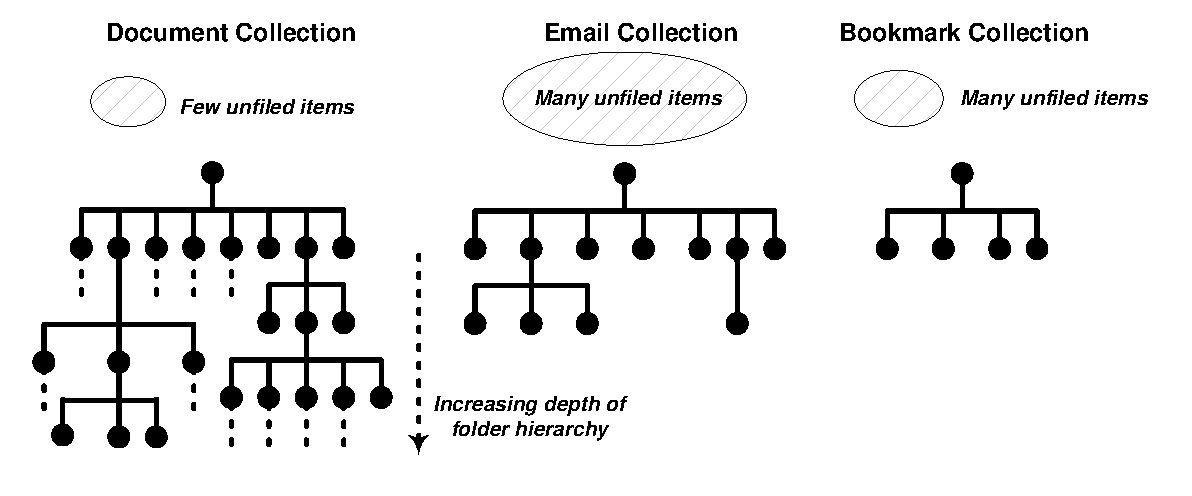
\includegraphics[width= \textwidth]{pictures/exp-study/exp-study-OrgComparison.pdf}
%		\caption{Comparison of the typical form of folder hierarchies developed in each PIM collection}
%		\label{fig:chapter1_collection_forms}
%	\end{center}
%\end{figure}
%%%%%%%%%%%%%%%%%%%%%%%%%%%%%%%%%%%%%%%%%%%%%%%%%%%%%%%%%%%%
% In the conceptual overview of PIM presented in \textbf{Chapter~\ref{chapter:introduction}}, two forms of organization were considered: (1) \textit{implicit} organization based on system-assigned metadata, (2) \textit{explicit} organization performed by the user (e.g. classifying items within folders or spatially grouping items on the desktop).
% The study focused on participants' explicit folder-based organizing behaviour, rather than reliance on implicit metadata or the use of the desktop to spatially organize items.
% Overall the document file collection tended to be structured much more extensively with the vast majority of items filed within folders for most users. 
% On average the file folder hierarchies were almost twice as deep as the email and web bookmark hierarchies (see \textbf{Table~\ref{table:chapter3_organization_strategy}}). 
\textbf{Table~\ref{table:chapter3_organization_strategy}} shows an overview comparison of organizing behaviour across the 3 PIM-tools. This analysis is based on the qualitative data and initial analysis of the folder structures.

%%%%%%%%%%%%%%%%%%%%%%%%%%%%%%%%%%%%%%%%%%%%%%%%%%%%%%%%%%
% TABLE: Comparing organizing characteristics of file, email and bookmarks}
%%%%%%%%%%%%%%%%%%%%%%%%%%%%%%%%%%%%%%%%%%%%%%%%%%%%%%%%%%
% CONSIDER ADDING: Consider use of large/small categories, default folders
% Barreau: different classifying rules based upon level of granularity to support in workload
\begin{table}[hbtp]
\begin{center}
\begin{footnotesize}
\setlength{\extrarowheight}{2pt}
\begin{tabular}{|p{2.5cm}|p{3.5cm}|p{3.5cm}|p{3.5cm}|}
% Table generated by Excel2LaTeX from sheet 'ORGANIZATION'
\hline
    {\bf } & {\bf Document File} & {\bf Email} & {\bf Web Bookmark} \\
\hline
{\bf Participants with active folders} &   {\it 25} &   {\it 23} &   {\it 16} \\
\hline
{\bf Average number of folders} & {\it 49 (SD: 30, min: 5, max: 122)} & {\it 37 (SD: 41, min: 0, max: 181)} & {\it 12 (SD: 15, min: 0, max: 55)} \\
\hline
{\bf Average maximum depth of folders} & {\it 3.0 (SD: 1.6, min: 1, max: 7)} & {\it 1.7 (SD: 1.2, min: 0, max: 4)} & {\it 1.1 (SD: 0.9, min: 0, max: 3)} \\
\hline
{\bf Average number of unfiled items} & {\it 65 (SD: 104, min: 0, max: 340)} & {\it 777 (SD: 1235, min: 7, max: 5577)} & {\it 43 (SD: 47, min: 0, max: 200)} \\
\hline
{\bf Most common organizing behaviour} & "One touch" file-on-creation. Occasional spring-cleaning..  & Some incremental filing but many left in inbox.  Use of filters to file mailing lists. Occasional spring-cleaning..  & Mostly left in default chronological order. Occasional spring-cleaning. Folder structures often abandoned. \\
\hline
{\bf Extent of filing} & High: most files organized in folders. & Variable. Large number of unfiled items in "inbox". & Majority in chronologically ordered list. \\
\hline
{\bf Location of "active" items} & Most active files located in folders. Some participants had unfiled "work-in-progress" area. & Inbox. Occasional project folders. & Most likely to be recently added unfiled items. \\
\hline
{\bf Other  organizing mechanisms (non-folder based) } & Spatial placement on desktop. Use of different  drives and partitions. & Occasional separation of roles between different email accounts. & Occasional spatial placement on desktop. Use of ``links bar''. \\
\hline
{\bf Key  problems} & Anxiety of order. Keeping collection tidy (unfiled items, pruning folders).  & Anxiety of order (focused on size of inbox). & Anxiety of order. Time to organize outweighs value of doing so (items rarely used again). Poor interface. \\
\hline
\end{tabular}  
\end{footnotesize}
\caption{Comparing organizing behaviour between files, email and bookmarks}
\label{table:chapter3_organization_strategy}
\end{center}
\end{table}

% Also consider use of command-line
% Note that other collections of personal information such as contacts and to-do items were rarely organized explicitly.
% Since organizing strategies varied significantly between the collections, WE present each in turn, starting with files.
%%%%%%%%%%%%%%%%%%%%%
% FOCUS ON FOLDERS
%%%%%%%%%%%%%%%%%%%%%
By far the dominant organizational mechanism employed was the folder hierarchy which acts as the focus of this section.  However, desktop icons were also used by many users to manage document files or web bookmarks on a temporary ``work in progress'' basis.  Although organizing behaviour varied between participants, common approaches stood out for each type of information.

%%%%%%%%%%%
% FILES
%%%%%%%%%%
As shown in \textbf{Table~\ref{table:chapter3_organization_strategy}}, most participants organized files most extensively, with deeper folder hierarchies, and fewer unfiled items compared to the other collections\footnote{An item was considered to be \textit{unfiled} if it was located on the desktop or in the root folder.}.  On average, participants had 49 file folders, as opposed to 37 in email, and 12 in bookmarks.

%%%%%%%%%%%%%%%%%%%%%%%%%%%%%%%%%%%
% COMPARE IN TERMS OF ACTIVE USE
%%%%%%%%%%%%%%%%%%%%%%%%%%%%%%%%%%%
% During the study, the number of folders in active use was estimated based on participant comments. 
Furthermore, a greater proportion of file folders were estimated to be in active use.  Although no detailed measures were taken, this appeared true for most participants, based on their comments.  An active folder was defined as one in which an item had been filed into, or retrieved from over the past week.  In particular, many participants mentioned that their web bookmark folders were old and/or redundant. An interesting further experiment would be to harvest detailed folder currency information.
% Overall more of the document file and email folders tended to be in active use compared to the web bookmark folders.

%%%%%%%%%%%
% EMAIL
%%%%%%%%%%%
% Participants were generally less reliant on folders in their email collection, and only twenty of the participants had folders that were in active use.  % The average number of folders was lower than in the document collection (34.1 compared to 42.6).
During the guided tours of email, participants talked about organization in terms of keeping their inbox tidy.  This \textit{inbox-focused} organizing tended to be as much about deleting items as filing them away.  The participants indicated that their inboxes often got ``out of control'' so incremental organizing was backed-up with occasional spring-cleans, e.g. P13: \textit{``I try and file systematically but right now my inbox is pretty big because I had no time over Christmas''}.
% The most common user strategy was a combination of incremental deletion and filing of messages when they were ``dealt with'' (e.g. read or replied to).
% Several participants (\textit{COUNT}) also used filters to automatically delete or file certain messages
% Five participants did not file email. Instead they relied on implicit metadata-based organization to help them locate items.




%%%%%%%%%%%%%%%%%%%%%
% SPRING-CLEANING
%%%%%%%%%%%%%%%%%%%%
% However most participants carried out occasional tidying on their collections of personal information.  Tidying was either carried out at the file-level (filing, deleting files), at the folder-level (reorganizing folders), or globally (``spring-cleaning'' the entire collection). 
% Most participants carried out some form of spring-cleaning on an occasional basis.
% TIDYING FROM OLD MAINT:   Incremental: a) folder containing too many items - therefore split into sub-categories, b) folder containing too few items (failed folder) -- remove, c)  duplicate folders - merge, d) lose something - improve filing system. 
Spring-cleaning was most commonly referred to in the context of email and was typically focused at filing and/or deleting items in the inbox once it had reached a certain size.  Spring-cleaning appeared to be less common in the document file context where items were typically organized incrementally. For those participants for whom tidiness was important, spring-cleaning was typically initiated when a collection reached a certain level of messiness.  Others were more pragmatic and spring-cleaned when they failed to find an item, e.g. P18: \textit{``If I lose something, then I make the hierarchy richer''}.

%%%%%%%%%%%%%
% BOOKMARKS
%%%%%%%%%%%%%
Bookmark collections were of little value to many participants, P2: \textit{``I have lots of unfiled bookmarks as they're hard to file. I could go through and delete them but not high-priority.''}. Four participants reported completely restarting bookmark collections rather than devote time to organizing them. However,  interestingly, they would then proceed to start the collection again using similar folders as before. % LINK TO IRRATIONAL

%%%%%%%%%%%%%%%%%%%%%%%%%%%%%%
% Location of active items
%%%%%%%%%%%%%%%%%%%%%%%%%%%%%%
Organizing strategies influenced how active items were distributed in each collection.  Active document files tended to be scattered around a set of active folders.  Some participants also stored active document files on the desktop on a temporary basis however in many cases these were never cleared away. Active email messages tended to be heavily concentrated in the inbox.  Thus messages related to different roles and projects were interleaved in the same list, along with newly arrived messages yet to be processed. % Cue overheads of inbox management.
Active bookmarks tended to be those added to the root level most recently. % But accessed relatively rarely



%%%%%%%%%%%%%%%%%%%%%%%%%%%%%%%%%%%%%%%%%%%%%%%%%
% User disposition towards filing
%%%%%%%%%%%%%%%%%%%%%%%%%%%%%%%%%%%%%%%%%%%%%%%%%
Two high-level attitudes could be identified towards organizing:
\begin{itemize}

\item \textit{Pro-organizing attitude} -- Several participants perceived distinct benefits in being tidy, P11: \textit{``These are ongoing projects which I like to keep tidy as they could be of future importance. Having an organized computer has clear benefits for future research by making it easy to find and read stuff when you need it again''}.  

\item \textit{Organizing-neutral attitude} -- Other participants were less driven to organize, e.g. P6: \textit{``I'd characterise myself as being (1) busy and (2) lazy. I need to carefully prioritize my time with a bias towards (1) fun, and (2) must-do/sense of duty.  Since PIM isn't either of these I don't do it''}. Several participants indicated that organizing was a complete waste of time, P19: \textit{``I've just happened to start filing as an experiment.  But I worry that its just like filing trash -- like having a tidy waste paper basket''}.
% In terms of tidying, some participants were proud of the fact that they had not tidied their files since they had started collecting them!

\end{itemize}

%%%%%%%%%%%%%%%%%%%%%%%%%%%%%
% Relate to rest of chapter
%%%%%%%%%%%%%%%%%%%%%%%%%%%%%
Participants tended to be more pro-organizing in files, and more organizing-neutral in email and bookmarks.

Several other sets of findings later in this chapter focus on organizing behaviour.   \textbf{Section~\ref{exp-study:Results-org-strategies}} presents a systematic investigation of the consistency of participants's organizing behaviour across the three PIM-tools.  New tool-specific and cross-tool classifications of participants' organizing strategies are offered. 
% \textbf{Section~\ref{exp-study:Results-org-strategies}} develops detailed classifications of participants' organizing strategies.
% focuses on organizing, and profiles participants in terms of which PIM-tools they were pro-organizing or organizing-neutral in.
Then, \textbf{Section~\ref{exp-study:Results-org-dims}} compares the folder structures in terms of their \textit{organizational dimensions}, and \textbf{Section~\ref{exp-study:Results-folder-overlap}} reports the amount of folder overlap between different tools. 



%%%%%%%%%%%%%%%%%%%%%%%%%%
% OTHER STUFF - REMOVED
%%%%%%%%%%%%%%%%%%%%%%%%%%

%%%%%%%%%%%%%%%%%%%%%%%%%%%%%%%%%%%%%
% Comparison with previous studies
%%%%%%%%%%%%%%%%%%%%%%%%%%%%%%%%%%%%%
% The results can be compared with those from previous studies, and were broadly in line (for example the average number of email folders in Duchaneaut \& Bellotti's study was 400 with a median result of 27~\citep{Ducheneaut:01}.  The need for more empirical work is expressed due to the variability of results: PIM is highly idiosyncratic.
% Duchaneaut and Bellotti also observe a correlation between email experience and number of folders. Although this relationship was not rigorously analysed here, several experienced participants had very few folders - possibly questioning the generality of Duchaneaut and Bellotti's result. \textit{THINK: WHY LOWER HERE ?}
% DEPTH FILES: This did not tie in with results from other user studies including (Barreau and Nardi 1995). 
% Barreau: different classifying rules based upon level of granularity to support in workload

%%%%%%%%%%%%%%%%%%
% USES OF FOLDERS
%%%%%%%%%%%%%%%%%%
% Filing tended to be seen as something that aided in retrieval.  Tendency to file if greater perceived value of information (e.g. important information, if easier to file, or if higher perceived chance of retrieving it again). However, there were other uses for folders beyond facilitating later retrieval. These ``contextualizing'' uses of folders include acting as reminders, or packaging up items for knowledge transfer. % Observed contextualizing uses of personal information are listed in \textbf{Table~\ref{table:contextualising_uses}}.

%%%%%%%%%%%%%%%%%%%%%%%%%%%%%%%%%%%%%%%%%%%%%%%%%%%%%%%%%%%%%%%%
% Contextualizing uses (e.g. use as reminders)}
%%%%%%%%%%%%%%%%%%%%%%%%%%%%%%%%%%%%%%%%%%%%%%%%%%%%%%%%%%%%%%%%
%\begin{table}[hbtp]
%\begin{center}
%\begin{footnotesize}
%\setlength{\extrarowheight}{2pt}
%\begin{tabular}{|p{2.5cm}|p{3.5cm}|p{3.5cm}|p{3.5cm}|}
%\hline
%    {\bf } & {\bf Document File} & {\bf Email} & {\bf Web Bookmark} \\
%\hline
%{\bf Contextualizing uses (beyond storage and retrieval)} & Reminders (desktop icons) & Reminders (inbox), Document transfer, scheduling/time management &     Little \\
%\hline
%{\bf Reminders/task/time-management} & Implicit reminders of things to do and work in progress. Often located in particular "work in progress" folder or as desktop icons. & Reminders typically listed in inbox. Occasional use of explicit to-do marking facility & Reminders of sites to check out, but typically user never does \\
%\hline
%{\bf Auditing, record of work done} &        yes &        yes &            \\
%\hline
%{\bf Knowledge transfer} & packaging up  (grouping files for transfer) & Transferring documents to others &            \\
%\hline
%{\bf Ideas, brainstorming} &            &   yes (sj) &            \\
%\hline
%{\bf Ad-hoc lists} & cf. within item in content, and in terms of separate items &            &            \\
%\hline
%{\bf Version control, archiving of old data} & file and folder level & threading-based &            \\
%\hline
%\end{tabular}  
%\end{footnotesize}
%\caption{Contextualizing uses of the document file, email and web bookmark collections beyond storage and retrieval}
%\label{table:contextualising_uses}
%\end{center}
%\end{table}


% The \textit{tool-specific} strategy classifications proposed in this section are employed in the \textit{cross-tool profiling} analysis in \textbf{Section~\ref{exp-study:Results-cross-tool-profiling}}.










%%%%%%%%%%%%%%%%%%%%%%%%%%%%%%%%%%%%%%%%%%%%%%%%
\subsection{Maintenance}
\label{exp-study:comparison-maintenance}
%%%%%%%%%%%%%%%%%%%%%%%%%%%%%%%%%%%%%%%%%%%%%%%%
% ADD TO DISCUSSION?
% Consider relationship between maintenance and organization
% ADD: Knock-on problem of archiving: means that its harder to find.
%% Could add much more detail, here or in discussion: TODO: contrast Barreau (95) and Whittaker (96) usage of the word "archive". WE use Barreau's interpretation - archiving as removing an item from a collection and placing it in separate storage, i.e. more than just placing it an easily accessible folder. Propose tighter definition of archive - for some people file = archive, but Barreau's interpretation was removing items from the collection and archiving remotely.
%% Also remember that Barreau included updating of items in maintenance
%% Note that the specific uses to which information is applied (e.g. editing a report) is outside the bounds of PIM).
%% Relate PIM and IR.
%%%%%%%%%%%%%%%%%%%%%%%%%%%%%%%%%%%%%%%%%%%%%%%%%%%%%%%%%%%%%%%%%%%%%%%%%%%%%%%%%%%%%%%%%%%%%
% In this section WE compare maintenance practices between the three collections. 
%%%%%%%%%%%%%%%%%%%%%%%%%%%%%%%%%%%%%%%%%%%%%%%%%%%%%%%%%%%%%%%%%%%%%%%%%%%%%%%%%%%%%%%%%%%%%%
% TIDYING STUFF FOR ORG
% 	\item \textbf{tidying} -- at the file-level, at the folder-level, or global ``spring-cleaning'' of the entire collection
% These findings add to previous evidence that maintenance is of low priority~\citep{barreau:95}. 
%%%%%%%%%%%%%%%%%%%%%%%%%%%%%%%%%%%%%%%%%%%%%%%%%%%%%%%%%%%%%%%%%%%%%%%%%%%%%%%%%%%%%%%%%%%%%%%%
Although most participants acknowledged the worth of maintenance, they did not devote much time towards it in any of the three three collections.  \textbf{Table~\ref{table:chapter3_maintenance_strategy}} compares observed maintenance practices between the collections.  %The following types of maintenance activity were encountered during the study:
%\begin{enumerate}
%\item \textit{Deletion} -- 
%\item \textit{Archiving} -- removing a portion of the collection and placing it in separate storage.
%\item \textit{Making back-ups} -- making a copy of the collection.
%\item \textit{synchronization} -- mirroring the collection to another computer.
%\end{enumerate}

\begin{table}[hbtp]
\begin{center}
\begin{footnotesize}
\setlength{\extrarowheight}{2pt}
\begin{tabular}{|p{2.5cm}|p{3.5cm}|p{3.5cm}|p{3.5cm}|}
\hline
    {\bf } & {\bf Document File} & {\bf Email} & {\bf Web Bookmark} \\
\hline
{\bf Deletion} & Occasional. & Incremental deletion of messages from inbox. Also occasional spring-cleaning. & Rare. More likely to abandon entire collection \\
\hline
{\bf Archiving} & Much of collection is effectively archived in situ. Users archive additional files into collection. & For some participants: occasional in-situ archiving of inbox or sent messages. & Not encountered. \\
\hline
{\bf Backing-up} & Manual backing-up for important files. Use of automatic mechanisms rare. & Rare. Some participants left a copy of all messages on server. & Not encountered. \\
\hline
{\bf Synchronization} & Occasionally performed manually between computers. & Some participants downloaded in parallel on multiple machines. & Not encountered. \\
\hline
\end{tabular}  
\end{footnotesize}
\caption{Comparing maintenance behaviour between files, email and bookmarks}
\label{table:chapter3_maintenance_strategy}
\end{center}
\end{table}


% ARCHIVING Most items in the collections were effectively archived in situ, lots of space, no need to archive them. There was some concern at the poor accessibility of archived material. Again archiving was most common for those participants for whom tidiness was important, i.e. those who were \textit{organizing-positive}, e.g. P1: \textit{``After the project finished it was 99\% useless stuff. I just wanted to get it out of the way''}.
Old items were rarely archived out of the collections. It was more common for archiving to be \textit{in situ}.  For example several participants occasionally purged old emails from the inbox to a local ``old-inbox'' folder.  Thus collections tended to include a mix of ephemeral, working and archived information.  One reason for this was the perceived difficulty in retrieving archived items. Most participants reported that extensive archiving only occurred during major life change stages such as starting a new job, or changing computer.  Due to the availability of cheap storage, space appeared to be less of an issue than in previous studies~\citep{barreau:95}.  Only 4 participants reported archiving portions of the file or email collections when they ran out of space, e.g. P21: \textit{``There's a lot of stuff that shouldn't have been there ... I need to tidy up, I'm always out of memory''}.

%%%%%%%%%%%%%%%%%%%%
% BACKING-UP/SYNCH
%%%%%%%%%%%%%%%%%%%%
% most commonly observed when it was automatic, for instance the automatic backing-up of a network drive.   However this meant that certain participants had lost data (e.g. P7). A number of participants expressed the wish for improved synchronization support. Currently carried out in an ad-hoc manner (e.g. by email). Most common for document files. Although participants mentioned that they would also like it for email and bookmarks.
Backing-up and synchronization were rarely observed.  Occasionally, highly important work was backed up manually.  In several cases this was in response to a previous loss of data.  Many participants expressed a desire for automatic mechanisms.

%%%%%%%%%%%%%%%%%
% SATISFICING
%%%%%%%%%%%%%%%%%
% Instead, it was performed in a satisficing manner. 
In general, these findings confirmed previous observations that maintenance is performed regularly but is instead carried out in reaction to events such as data loss, lack of space, and life changes~\citep{barreau:95}.




%%%%%%%%%%%%%%%%%%%%%%%%%%%%%%%%%%%%%%%%%%%%%%%%%%%%%
\subsection{Retrieval}
\label{exp-study:comparison-retrieval}
%%%%%%%%%%%%%%%%%%%%%%%%%%%%%%%%%%%%%%%%%%%%%%%%%%%%%
% DISCUSSION: Postulate other reasons why users preferred browsing.  Serendipity. Visual. Incremental feedback. Familiarity

\textbf{Table~\ref{table:chapter3_retrieval_strategy}} summarizes the observations regarding retrieval behaviour.
%%%%%%%%%%%%%%%%%%%%%%%
% Browsing over search
%%%%%%%%%%%%%%%%%%%%%%%
Unlike acquisition and organization where greatly differing behaviour was observed across PIM-tools, some consistency was seen in retrieval practices. 
Participants reported a strong preference for \textit{browsing} over \textit{search} in all three tools. This cross-tool consistency supports and extends tool-specific findings in files~\citep{bn:95}\footnote{\citet{Gelernter:96b} suggested that a factor contributing to the rare usage of search may be poor implementation.  Participants' comments confirm this, suggesting that there has been little improvement in search implementation.}.  However, there was variation between the collections in terms of the type of browsing employed. Two types of browsing were encountered: (1) \textit{location-based browsing} of folders/desktop icons~\citep{bn:95}, and (2) the \textit{sorting/scanning} of items, ordered by user-defined metadata (e.g. \texttt{name}) or system-defined metadata (e.g. \texttt{size}).
%%%%%%%%%%%
% FILES
%%%%%%%%%%%
When retrieving files, participants employed a combination of both -- browsing to a folder, and then sorting items within it, e.g. P2: \textit{`` If I'm looking for something, I'll firstly browse about.  I only search as a last resort''}. Additionally, many participants employed application-history when working in tools such as MS-Word -- thus avoiding the need to browse or search.


\begin{table}[hbtp]
\begin{center}
\begin{footnotesize}
\setlength{\extrarowheight}{2pt}
\begin{tabular}{|p{2.5cm}|p{3.5cm}|p{3.5cm}|p{3.5cm}|}
% Table generated by Excel2LaTeX from sheet 'RETRIEVAL'
\hline
    {\bf } & {\bf Document File} & {\bf Email} & {\bf Web Bookmark} \\
\hline
{\bf Most common behaviour} & Browse (supported by sort). Search as last resort. & Sorting of items in inbox. Search as last resort. & Browse or frequent use of an alternate  mechanism  (e.g. search engine). \\
\hline
{\bf Likelihood of retrieval} & High. Biased towards  ``work in progress''. Occasional for older items. & High for recently added items in inbox. Low for older items. & Low. Bias towards recently added items. \\
\hline
{\bf Use of sorting} & Sorting: alphabetical, creation-date, format. & Sorting: date received, author. & No sorting mechanisms provided. Left in default chronological ordering.  \\
\hline
{\bf Alternate retrieval mechanism} & Use of application history  (e.g. MS-Office). & Use of on-line mailing list archives. Asking sender to resend as last resort. & Frequently use of: web search engine, browser history, URL `auto-completion. \\
\hline
{\bf Key retrieval problems} & Failure to find highly frustrating but rare. Slow integrated search & Failure to find an item highly frustrating but rare. Slow integrated search & Poor browsing interface. Lack of search.  \\
\hline
\end{tabular}  
\end{footnotesize}
\caption{Comparing retrieval behaviour between files, email and bookmarks}
\label{table:chapter3_retrieval_strategy}
\end{center}
\end{table}





%%%%%%%%%%%%%%
% EMAIL
%%%%%%%%%%%%%%
For email, retrieval was focused on sorting/scanning the inbox - location-based browsing of folders was less common. Search was used more in email than in files, but was still seen as a last resort by most participants in both collections: P25: \textit{``I usually know exactly where I'm going and what I'm looking for. If I search I wouldn't necessarily know the exact keyword. If you know where you're going, browsing is a lot quicker''}.
% Rather than searching items by metadata or content, users expressed a strong preference for browsing which was seen as the faster alternative.

%\begin{quote}
%P2 (EMAIL): \textit{``I try to minimise structure as I find by sorting on date and sender metadata to get a flexible view.  Then I search if I can't find it.''}
%\end{quote}

%\begin{quote}
%P21 (EMAIL): \textit{``When I'm findings things [messages] first I'll browse for a minute or so. If that doesn't work then I'll search, but that's so slow.''}
%\end{quote}

%%%%%%%%%%%%%%
% BOOKMARKS
%%%%%%%%%%%%%%
Bookmark retrieval was focused on scanning recently added, or frequently accessed items. However, several participants stated that they preferred to search the web again rather than find a bookmark: P18: \textit{``If something is really exciting then I bookmark it ... when I come back to it, I just use Google''}. Nevertheless, participants continued to save bookmarks, even though many were never used. Similar behaviour was observed in email, in particular collecting/filing messages from mailing lists, which were never read: P16: \textit{``Of the emails you do save, 90\% you never read again''}. Similar ``irrational'' behaviour, pointing to an innate need to acquire, has been observed in paper archives, e.g. keeping personal copies of items that are publicly available~\citep{Whittaker-paper:01}.
% SCRATCH: None of the bookmark interfaces encountered provided a search mechanism, and in fact most users indicated that they did not often retrieve the bookmarks they stored. If bookmarks were retrieved they were typically those added most recently or one or two frequently-used links. Instead users were more likely to use an alternate mechanism for accessing web pages such as a search engine.  Despite the lack of preference for search in document files and email, interestingly several participants complained about the lack of a search facility in their bookmark tool.

%%%%%%%%%%%%%%%%%%%%%%%%%%%%%
% People retrieve old stuff
%%%%%%%%%%%%%%%%%%%%%%%%%%%%%
In all three collections, retrieval was biased towards active and/or recently added items. However, many participants mentioned tasks that required access to older information, archived in situ, e.g. P22: \textit{``You look at what exam questions you had for the previous years and you decide to recycle a question or two''}. This finding is not consistent with previous claims that archived information is not useful to people\citep{bn:95}. This suggests that although older items were only accessed erratically, they can be highly valued by people, supporting findings in~\citep{Whittaker-paper:01}.

Interestingly, in all three collections failure to find items appeared to happen only occasionally: P18: \textit{``If it exists then I'll find it. The only cases I don't is when I deleted it because I thought I didn't need it again''}. Participants expressed confidence that in general they ``just knew'' where to find items. However, those rare occasions when they could not find items were highly frustrating. Three main reasons were cited for failure: (1) deleting/archiving items, (2) clutter, and (3) misfiling.
% Interestingly findings items did not appear to be as much of a problem as the issue of ``anxiety of order'' reported in \textbf{Section~\ref{exp-study:qual_organization}}. Users reported that they were able to find items when they needed them on most occasions. However those times when they failed to locate items were quite rare, they were very frustrating.
Several participants reported looking for items for up to ten minutes before resorting to an alternative method (e.g. asking a correspondent to resend an email).
%\begin{quote}
%	\textit{INSERT participant 22's comment of not being able to find item of email and the consequence of that!}
%\end{quote}


%%%%%%%%%%%%%%%%%%%%%%%%%%%%%%%%%%%%%%
% \subsubsection{Summary comparison}
%%%%%%%%%%%%%%%%%%%%%%%%%%%%%%%%%%%%%%
%%%%%%%%%%%%%%%%%%%%%%%%%%%%%%%%%%%%%%%%%%%%%%%%%%%%%%%%%%%%
% TO ADD: WHY WAS THIS DONE? WHAT IS THE MAIN CONCLUSION?
%%%%%%%%%%%%%%%%%%%%%%%%%%%%%%%%%%%%%%%%%%%%%%%%%%%%%%%%%%%%




%%%%%%%%%%%%%%%%%%%%
\subsection{Discussion}
\label{exp-study:Results-comparison-summary}
%%%%%%%%%%%%%%%%%%%%
%	\item Reinforce key findings
%	\item Link to next section
%	\item THINK: avoid overlap with discussion at end
%%%%%%%%%%%%%%%%%%%%%%%%%%%%%%%%%%%%%%%%%%%%%%%%%%%%%%%%%%%%
% TO ADD: WHY WAS THIS DONE? WHAT IS THE MAIN CONCLUSION?
%%%%%%%%%%%%%%%%%%%%%%%%%%%%%%%%%%%%%%%%%%%%%%%%%%%%%%%%%%%%

The previous four sections have contrasted acquisition, organizing, maintenance and retrieval behaviour across files, email and bookmarks.  \textbf{Table~\ref{table:chapter3_overview_strategy}} provides a summary of the most commonly observed strategies. % The classifications of tool-specific strategies are used in the cross-tool profiling analysis in \textbf{Section~\ref{exp-study:Results-cross-tool-profiling}}.

\begin{table}[hbtp]
\begin{center}
\begin{footnotesize}
\begin{tabular}{|p{2.5cm}|p{3.5cm}|p{3.5cm}|p{3.5cm}|}
% Table generated by Excel2LaTeX from sheet 'HIGH_LEVEL STRATEGY OVERVIEW'
\hline
    {\bf } & {\bf Document File} & {\bf Email} & {\bf Web Bookmark} \\
\hline
{\bf Acquisition} & Manual. User decides what to add. & Automatic. User must decide what to keep. & Manual. User decides what to add. \\
\hline
{\bf Organization} & File-on-creation. Some working or temporary files managed on the desktop. Occasional spring-cleaning. & Focused on inbox. Incremental filing and spring-cleaning. & Occasional filing. Many items left in default chronological list. \\
\hline
{\bf Maintenance} & Occasional. & Incremental deleting of old items in inbox. & Rare. Many users abandon collection and start over. \\
\hline
{\bf Retrieval} & Preference for browse/sort over search. & Inbox-focused. Preference for sorting over search. & Focused on recently added items. Use of alternate mechanisms. \\
\hline
\end{tabular}  
\end{footnotesize}
\caption{Summary Comparison of PIM Strategies in the three collections}
\label{table:chapter3_overview_strategy}
\end{center}
\end{table}

Although in many ways, the interface functionality provided in each PIM-tool is similar, the results point to many differences between typical user behaviour across the three PIM-tools.  A number of similarities were also highlighted, such as the preference for browsing over search in multiple tool contexts, and the satisficing nature of maintenance.

The findings reported in this section provided the author with an empirical foundation for the rest of the thesis work.  \textbf{Chapter~\ref{chapter:discussion}} argues that Barreau's conceptualization of the computer as a ``monolithic'' PIM system~\citep{barreau:95} should be extended to reflect the similarities and differences between behaviour in the different PIM-tools. Subsequently, a new perspective is proposed which conceptualizes the computer as a set of distinct PIM sub-systems.
% The  are used to argue for a 

%%%%%%%%%%%%
% LINK ON
%%%%%%%%%%%%
% The next three sections take a focus on organizing behaviour.  
% \textbf{Section~\ref{exp-study:Results-org-dims}} reports the analysis of organizational dimensions. \textbf{Section~\ref{exp-study:Results-folder-overlap}} reports the analysis of folder overlap.

%%%%%%%%%%%%%%%%%%%%%%%%%%%%%%%%%%%%%%%%%%%
%% END RESULTS1-COMPARISON/CHAPTER 4 EXP STUDY
%%%%%%%%%%%%%%%%%%%%%%%%%%%%%%%%%%%%%%%%%%%










%%%%%%%%%%%%%%%%%%%%%%%%%%%%%%%
% CHAPTER 4: EXPLORATORY STUDY
% 	RESULTS 2 - Organizational Dimensions
% File: tex/expstudy-chapter/expstudy-results1a-strategies.tex
%%%%%%%%%%%%%%%%%%%%%%%%%%%%%%%%%%%%%%%%%%%%%%%%
%%%%%%%%%%%%%%%%%%%%%%%%%%%%%%%%%%%%%%%%%%%%%%%%
%%%%%%%%%%%%%%%%%%%%%%%%%%%%%%%%%%%%%%%%%%%%%%%%

%%%%%%%%%%%%%%%%%%%%%%%%%%%%%%%
% CHAPTER 4: EXPLORATORY STUDY
% 	RESULTS 2 - Cross-tool profiling
% File: tex/expstudy-chapter/expstudy-results2-cross-tool-profiling.tex
%%%%%%%%%%%%%%%%%%%%%%%%%%%%%%%%%%%%%%%%%%%%%%%%
%%%%%%%%%%%%%%%%%%%%%%%%%%%%%%%%%%%%%%%%%%%%%%%%
%%%%%%%%%%%%%%%%%%%%%%%%%%%%%%%%%%%%%%%%%%%%%%%%
\newpage
\section{Results: Comparing Organizing Strategies}
\label{exp-study:Results-org-strategies}
%%%%%%%%%%%%%%%%%%%%%%%%%%%%%%%%%%%%%%%%%%%%%%%%
%%%%%%%%%%%%%%%%%%%%%%%%%%%%%%%%%%%%%%%%%%%%%%%%

The previous section provided a high-level comparison of PIM behaviour between files, email and bookmarks.  This section presents a more detailed comparison of organizing strategies.  \textbf{Section~\ref{exp-study:cross-tool-profiling}} describes the approach that was employed.
\textbf{Sections~\ref{exp-study:Results-org-strategies-files}}, \textbf{\ref{exp-study:Results-org-strategies-email}} and \textbf{\ref{exp-study:Results-org-strategies-bookmarks}} classify participants' behaviour in each PIM-tool in turn.  Then \textbf{Section~\ref{exp-study:Results-cross-tool-profiling}} reports the cross-tool profiling in which strategies were compared across tools.

% \textbf{Section~\ref{exp-study:Results-org-strategies}} reports the comparison of  on a user-by-user basis. % Key findings include the observation of the multiple PIM strategies employed by many participants in the 3 tools.  New classifications of behaviour are offered in each tool based on participants' reported filing strategies.
%Method described in . Two stages:
%\begin{enumerate}
%\item Characterize organizing behaviour in each PIM-tool in turn
%\item Compare organizing behaviour between the PIM-tool for each participant to investigate consistency 
%\end{enumerate}

% %%%%%%%%%%%%%%%%%%%%%%%%%%%%%%%%
% TOOL-SPECIFIC FINDINGS
%%%%%%%%%%%%%%%%%%%%%%%%%%%%%%%%
% Although not the main aim of the study, several incremental tool-specific contributions are offered including the new classifications of filing strategies reflecting the multiple strategies observed in each tool. 

%%%%%%%%%%%%%%%%%%%%%%%%%%%%%%%%%%%%%%%%%%%%%
\subsection{File Organizing Strategies}
\label{exp-study:Results-org-strategies-files}
%%%%%%%%%%%%%%%%%%%%%%%%%%%%%%%%%%%%%%%%%%%%%
% SCRATCH: Twenty-three of the twenty-five participants had document file folders in active use~\footnote{An active folder was defined as one containing items that were used in the last week/on a regular basis.}. Most of these participants pursued a \textit{file-on-creation} strategy with their document files: as items were created, users habitually filed them away (either using the file manager or the file dialog within editors such as MS Word).
% The most common profile was to organize most files as they were created, but to leave a small portion unfiled on the desktop or at the root level.

Since no classifications of file management strategies had been proposed in previous work, the author developed one from scratch based on participants' strategy descriptions. Three strategies were identified and are reported in \textbf{Table~\ref{table:exp-study:file_classification}}.

%%%%%%%%%%%%%%%%%%%%%%%%%%%%%%%%%%%%%%%%%%%%%%%%%%%%%%%%%%
% TABLE: A classification of file management strategies}
%%%%%%%%%%%%%%%%%%%%%%%%%%%%%%%%%%%%%%%%%%%%%%%%%%%%%%%%%%
% THINK: add overall average?
\begin{table}[hbtp]
\begin{center}
\begin{footnotesize}
\setlength{\extrarowheight}{2pt}
\begin{tabular}{|p{4cm}|c|c|c|}
% Table generated by Excel2LaTeX from sheet 'FS STRATS'
\hline
{\bf Strategy} & {\bf \# Users} & {\bf Average \# Folders} & {\bf Average \# unfiled items} \\
\hline
F1 total filers: file majority of items on creation. &         16 & 50 (SD: 29, min: 12, max: 122)  & 14 (SD: 9, min: 0, max: 30) \\
\hline
F2 extensive filers: file extensively, but leave many items unfiled. &          7 & 58 (SD:29, min: 5, max: 108) & 132 (SD: 137, min:  31, max: 340) \\
\hline
F3 occasional filers: file occasionally, leave most items unfiled, have few folders. &          2 & 5 (SD: 0, min: 5, max: 5) & 240 (SD: 127, min: 150, max: 330) \\
\hline
\end{tabular}  
\end{footnotesize}
\caption{Classification of observed file management strategies [n=25]}
\label{table:exp-study:file_classification}
\end{center}
\end{table}
\normalsize

23 of the 25 participants were \textit{pro-organizing}, and had extensive folder structures.  They could be divided into two groups (F1 and F2) based on the extent to which they employed a \textit{file-on-creation} strategy (filing new items immediately). F1 participants employed a predominantly file-on-creation strategy, and tended only to leave items unfiled by accident, except for a few temporarily placed work-in-progress files. F2 participants filed the majority of items on creation, but also managed a large unfiled subset of working/ephemeral items. F2 participants filed these items on completion of the relevant task, or during a spring-clean. Thus the location of ephemeral/working files varied between the two groups. F1 participants distributed them around active folders, whilst F2 participants left many unfiled. However, even for the F2 participants, unfiled items were a small proportion of their total collection.

The remaining two participants (group F3) were \textit{organizing-neutral}.  They filed less extensively, and stated that filing was not a priority.  In contrast most F1/F2 participants said that being organized was an important (though not always achievable) goal. 

%%%%%%%%%%%%%%%%%%%%%%%%
% MULTIPLE STRATEGIES
%%%%%%%%%%%%%%%%%%%%%%%
In addition. most participants occasionally performed spring-cleaning of their file collections. Note that most of the participants could not be described as filers or non-filers.  Instead, they employed \textit{multiple-strategies} -- filing some items on creation, leaving some unfiled, and carrying out occasional spring-cleaned. Multiple strategies were similarly observed in the other collections. % The next two sections also identify multiple strategies in the context of email and bookmarks respectively.






%%%%%%%%%%%%%%%%%%%%%%%%%%%%%%%%%%%%%%%%%%%%%%
\subsection{Email Organizing Strategies}
\label{exp-study:Results-org-strategies-email}
%%%%%%%%%%%%%%%%%%%%%%%%%%%%%%%%%%%%%%%%%%%%%%
% The author proposes a new classification of email management strategies based on the four observed strategies. The classification is summarized in Table~\ref{table:exp-study:email_classification} along with the characteristics of each class. 
% THINK: add overall average?

The author attempted to categorize participants' behaviour using previous classifications of email organizing behaviour~\citep{Whittaker-email:96,ob:97}. However, this was only a partial success. The sample included 2 \textit{no-filers} (folderless spring-cleaners), and 7 \textit{frequent filers} - but no \textit{spring-cleaners} (participants who only clean their inbox periodically).  The remaining 16 participants had large inboxes (>75 items, average 1137), like the no-filers and spring-cleaners in~\citep{Whittaker-email:96}, however their reported strategies did not match these classifications. They filed some new emails immediately (typically those of perceived long-term value such as e-commerce receipts), and deleted low-value spam. Other messages were left in the inbox, which was occasionally spring-cleaned.  In other words, as in files, they employed \textit{multiple strategies} - a combination of frequent filer, spring cleaner, and no-filer, e.g. P25: \textit{``I'd like to manage as and when I receive them but I don't. I do it periodically - 10 minutes a day just to categorize the things that are important. 10 or 15 I'll categorize ... the rest of them I think oh I'll get round to doing that at some stage - but I don't normally. However I did spend an hour on a train last week tidying my emails because I was bored. I reduced my inbox by about 1500''}.

A new classification was developed based on participants' strategy descriptions (see  \textbf{Table~\ref{table:exp-study:email_classification}}). The 16 \textit{multiple-strategy} participants could be divided into two sub-groups, E2 and E3, based on the extent to which they reported manually filing new messages on a daily basis. E2 participants filed many emails everyday, whilst E3 participants only filed a few (<5) messages of particular long-term value, P31: \textit{``I have a folder for registrations. I've got other [unused] folders - I don't even know what they are. The vast majority [of email] is a big long list''}. E1/E2 participants were pro-organizing, whilst E3/E4 participants considered it to be less important.



%%%%%%%%%%%%%%%%%%%%%%%%%%%%%%%%%%%%%%%%%%%%%%%%%%%%%%%%%%
% TABLE: A classification of email management strategies}
%%%%%%%%%%%%%%%%%%%%%%%%%%%%%%%%%%%%%%%%%%%%%%%%%%%%%%%%%%
\begin{table}[hbtp]
\begin{center}
\begin{footnotesize}
\setlength{\extrarowheight}{2pt}
\begin{tabular}{|p{4cm}|c|c|c|}
% Table generated by Excel2LaTeX from sheet 'EM STRATS'
\hline
{\bf Strategy} & {\bf \# Users} & {\bf Average \# Folders} & {\bf Average \# unfiled items} \\
\hline
E1 frequent filers: file or delete most incoming messages everyday. &          7 & 56 (SD: 62, min: 3, max: 181)  & 26 (SD: 15, min: 7, max: 50) \\
\hline
E2 extensive filers: try to file many messages everyday.  &         12 & 42 (SD: 24, min: 8, max: 91) & 1002 (SD: 1497, min: 87, max: 5577) \\
\hline
E3 partial filers: file only a few (<5) messages everyday.  &          4 & 4 (SD: 3, min: 0, max: 6) & 1251 (SD: 1254, min: 205, max: 3000) \\
\hline
E4 no-filers: do not file any messages. &          2 & 0 (SD: 0, min: 0, max: 0) & 1106 (SD: 1265, min: 211, max: 2000) \\
\hline
\end{tabular}  

\end{footnotesize}
\caption{Classification of observed email management strategies [n=25]}
\label{table:exp-study:email_classification}
\end{center}
\end{table}
\normalsize



 





%%%%%%%%%%%%%%%%%%%%%%%%%%%%%%%%%%%%%%%%%%%%%%
\subsection{Bookmark Organizing Strategies}
\label{exp-study:Results-org-strategies-bookmarks}
%%%%%%%%%%%%%%%%%%%%%%%%%%%%%%%%%%%%%%%%%%%%%%
%Bookmarks tended to be less structured than the other two collections with most items being left in a chronologically ordered list.  Less than half the participants had web bookmark folders in active use. 
% Several participants indicated that both web bookmarks and email had less value than document files and so were less worth organizing.

The author attempted to map participants' behaviour onto an existing classification~\citep{da:98}. However, as with email, the previous classification did not reflect the observed behaviour, and another new classification was developed (see \textbf{Table~\ref{table:exp-study:bookmark_classification}}).  Only 8 participants matched a previous classification, that of ``no filer''. 

%%%%%%%%%%%%%%%%%%%%%%%%%%%%%%%%%%%%%%%%%%%%%%%%%%%%%%%%%%
% TABLE: A classification of bookmark management strategies}
%%%%%%%%%%%%%%%%%%%%%%%%%%%%%%%%%%%%%%%%%%%%%%%%%%%%%%%%%%
% THINK: add overall average?
\begin{table}[hbtp]
\begin{center}
\begin{footnotesize}
\setlength{\extrarowheight}{2pt}
\begin{tabular}{|p{4cm}|c|c|c|} % total 13
\hline
{\bf Strategy} & {\bf \# Users} & {\bf Average \# Folders} & {\bf Average \# unfiled items} \\
\hline
B1 extensive filing: file many bookmarks as they are created or at the end of browsing session &          6 & 31 (SD: 16, min: 13, max: 55)  & 24 (SD: 19, min: 10, max: 40) \\
\hline
B2 partial filing: file bookmarks sporadically  &         10 & 10 (SD: 7, min: 3, max: 24) & 35 (SD: 32, min: 7, max: 120) \\
\hline
B3 no-filers: never file, all folders abandoned. &          8 & 1 (SD: 2, min: 0, max: 5) & 71 (SD: 67, min: 4, max: 200) \\
\hline
B4: non-collector &          1 &    {\bf -} &    {\bf -} \\
\hline
\end{tabular}  
\end{footnotesize}
\caption{Classification of observed bookmark management strategies [n=25]}
\label{table:exp-study:bookmark_classification}
\end{center}
\end{table}
\normalsize

The remaining 16 active collectors of bookmarks instead employed \textit{multiple strategies}. They filed a subset of bookmarks on creation, leaving others unfiled, often as reminders, until they were spring-cleaned or simply abandoned, \textit{P12: ``The main thing is a mess and completely littered with things. The only exception is when I mirrored web pages for experiments. Also I keep a folder with homepages''}. The multiple-strategy participants were divided into two groups, B1 and B2, based on the extent to which they reported filing new bookmarks on creation. Organization was of lower priority for the B2 participants who had fewer folders and more unfiled bookmarks.

% Note that in all three tools, most participants employed \textit{multiple-strategies}.


%%%%%%%%%%%%%%%%%%%%%%%%%%%%%%%%%%%%%%%%%%%%%%%%%%%%%%%%%%%%%%%%%%%%%%%%%%%%%%%%%%%%%%%%%%%%%%%%
%%%%%%%%%%%%%%%%%%%%%%%%%%%%%%%%%%%%%%%%%%%%%%%%%%%%%%%%%%%%%%%%%%%%%%%%%%%%%%%%%%%%%%%%%%%%%%%%
%%%%%%%%%%%%%%%%%%%%%%%%%%%%%%%%%%%%%%%%%%%%%%%%%%%%%%%%%%%%%%%%%%%%%%%%%%%%%%%%%%%%%%%%%%%%%%%%
%%%%%%%%%%%%%%%%%%%%%%%%%%%%%%%%%%%%%%%%%%%%%%%%%%%%%%%%%%%%%%%%%%%%%%%%%%%%%%%%%%%%%%%%%%%%%%%%


%%%%%%%%%%%%%%%%%%%%%%%%%%%%%%%%%%%%%%%%%%%%%%%%
%%%%%%%%%%%%%%%%%%%%%%%%%%%%%%%%%%%%%%%%%%%%%%%%
\subsection{Cross-tool Profiling}
\label{exp-study:Results-cross-tool-profiling}
%%%%%%%%%%%%%%%%%%%%%%%%%%%%%%%%%%%%%%%%%%%%%%%%
%%%%%%%%%%%%%%%%%%%%%%%%%%%%%%%%%%%%%%%%%%%%%%%%

%%%%%%%%%%%%%%%%%%%%%%%%%
% intro and structure
%%%%%%%%%%%%%%%%%%%%%%%%%
% *** Earlier section: compared PIM strategies (acquisition, organization, maintenance and retrieval) across tools.  high-level similarities and differences
% *** Previous studies have attempted to classify users based on their PIM strategies within particular tools, particularly with respect to filing strategies~\citep{da:98,Whittaker-email:96}. Why did they do this?
% *** Rationale: complex set of strategies and data. Attempt to summarize
%	*** The intention here was to investigate dependency on filing from a workspace-wide/cross-tool perspective
% Participants were profiled in terms of which tools they reported making significant filing effort in.
% based on the extent to which users devote effort to organizing the three types of information. The specific measure employed was how consistent   participants were in terms of reported filing behaviour. % The method used is discussed in \textbf{Section~\ref{exp-study:cross-tool-profiling}}. 
% *** Here WE attempt to classify users in terms of their \textit{cross-tool} approach to filing.  WE propose a new user classification based on the extent to which they organized multiple types of information within folders.  
This section presents the results from the cross-tool profiling analysis.  The aim of this analysis was to investigate the consistency of each participant's approach to organizing files, email and bookmarks. % This section goes beyond the analysis in \textbf{Section~\ref{exp-study:Results-comparison}} by attempting to build up a \textit{cross-tool} profile on a user-by-user basis, rather than generalizing across participants. 

%%%%%%%%%%%%%%%%%%%%%%%%%%%%%%%%%%%%%%%%%%%%%%%%%%%%%%%
% TABLE: table of tool-specific strategies
%%%%%%%%%%%%%%%%%%%%%%%%%%%%%%%%%%%%%%%%%%%%%%%%%%%%%%%
\begin{table}[btp]
\begin{center}
\begin{footnotesize}
\setlength{\extrarowheight}{2pt}
\begin{tabular}{|c|c|c|c|c|}
\hline
        \textbf{Participant} &       \textbf{File strategy} &         \textbf{Email strategy} &         \textbf{Bookmark strategy} & \textbf{Cross-tool profile} \\
\hline
         P1 &         F1 &         E2 &         B2 &        CT2 \\
\hline
         P2 &         F1 &         E2 &         B1 &        CT1 \\
\hline
         P3 &         F2 &         E2 &         B3 &        CT2 \\
\hline
         P4 &         F1 &         E3 &         B3 &        CT3 \\
\hline
         P5 &         F2 &         E2 &         B2 &        CT2 \\
\hline
         P6 &         F3 &         E3 &         B3 &        CT4 \\
\hline
         P7 &         F3 &         E4 &         B3 &        CT4 \\
\hline
         P8 &         F1 &         E3 &         B2 &        CT3 \\
\hline
         P9 &         F2 &         E2 &         B3 &        CT2 \\
\hline
        P10 &         F1 &         E4 &         B3 &        CT3 \\
\hline
        P11 &         F1 &         E1 &         B1 &        CT1 \\
\hline
        P12 &         F1 &         E1 &         B3 &        CT2 \\
\hline
        P13 &         F1 &         E2 &         B2 &        CT2 \\
\hline
        P14 &         F1 &         E1 &         B1 &        CT1 \\
\hline
        P15 &         F2 &         E2 &         B1 &        CT1 \\
\hline
        P16 &         F1 &         E2 &         B2 &        CT2 \\
\hline
        P17 &         F1 &         E1 &         B1 &        CT1 \\
\hline
        P18 &         F1 &         E2 &         B1 &        CT1 \\
\hline
        P19 &         F1 &         E2 &         B2 &        CT2 \\
\hline
        P20 &         F1 &         E2 &         B2 &        CT2 \\
\hline
        P21 &         F1 &         E1 &         B2 &        CT2 \\
\hline
        P22 &         F1 &         E1 &         B3 &        CT2 \\
\hline
        P23 &         F2 &         E1 &         B2 &        CT2 \\
\hline
        P24 &         F2 &         E3 &         B2 &        CT3 \\
\hline
        P25 &         F2 &         E2 &         B3 &        CT2 \\
\hline
\end{tabular}  
\end{footnotesize}
\caption{Table of participants' tool-specific strategies, and cross-tool profile}
\label{table:exp-study:tool-specific-classifications}
\end{center}
\end{table}
\normalsize

%%%%%%%%%%%%%%%%%%%%%%%%%%%%%%%%%%%%%%%
% \subsubsection{Method}
%%%%%%%%%%%%%%%%%%%%%%%%%%%%%%%%%%%%%%%
%%%%%%%%%%%%%%%%%%%%%%%%%%%%%%%%%%%%%%%%%%%
% 1. Table of the tool-specific strategies
%%%%%%%%%%%%%%%%%%%%%%%%%%%%%%%%%%%%%%%%%%%
%%%%%%%%%%%%%%%%%%%%%%%%%%%%%%%%%%%%%%%%%%%
% 2. Identification of cross-tool profile
%%%%%%%%%%%%%%%%%%%%%%%%%%%%%%%%%%%%%%%%%%%
The middle three columns of \textbf{Table~\ref{table:exp-study:tool-specific-classifications}} list the three \textit{tool-specific} strategies for each participant.  A cross-tool profile was then identified for each participant by collating the three strategies as a \textit{3-tuple}, e.g. \texttt{F1/E2/B2} for Participant P1. Across the twenty-five participants, fourteen unique tuples were identified.
%%%%%%%%%%%%%%%%%%%%%%%%%%%%%%%%%%%%%%%%%%%%%%%%%%%%%%%%%%%%%%%%%%%%%%%%%%%%%%%%%%%%%%%%%%%%
% 3. Classification of each set of tool-specific strategies based on extent of organizing
%%%%%%%%%%%%%%%%%%%%%%%%%%%%%%%%%%%%%%%%%%%%%%%%%%%%%%%%%%%%%%%%%%%%%%%%%%%%%%%%%%%%%%%%%%%%
The \textit{cross-tool profiles} were then clustered based on the following criterion:
\begin{quote}
\textit{In which of the three collections were the participants pro-organizing? (i.e. in which collections did they report making significant organizing effort?)}
\end{quote}

The first step of clustering the cross-tool profiles was to classify each set of tool-specific strategies as either \textit{pro-organizing} (involving high organizing effort) or \textit{organizing-neutral} (involving low organizing effort). This process was necessarily subjective since the nature of PIM in each tool varies, along with the objective criteria used to define the tool-specific strategy classifications.   Several classifications were attempted, from which the one shown in \textbf{Table~\ref{table:exp-study:strategy-classification}} emerged as the best match for the data. % THIS IS GOING TO NEED SOME ATTENTION! (-;

%%%%%%%%%%%%%%%%%%%%%%%%%%%%%%%%%%%%%%%%%%%%%%%%%%%%%%%
% TABLE: classifying the tool-specific strategies
%%%%%%%%%%%%%%%%%%%%%%%%%%%%%%%%%%%%%%%%%%%%%%%%%%%%%%%
%\begin{tabular}{|c|c|}
%\hline
%{\bf Tool-specific strategies} & {\bf Level of organizing effort} \\
%\hline
%F1/F2, E1/E2, B1 & ``Pro-organizing'', strategies that involve high organizing effort \\
%\hline
%F3, E3/E4, B2/B3 & ``Organizing-neutral'', strategies that involve low organizing effort \\
%\hline
%\end{tabular}  
\begin{table}[btp]
\begin{center}
\begin{footnotesize}
\setlength{\extrarowheight}{8pt}
\begin{tabular}{|c|c|c|c|}
\hline
{\bf Level of organizing effort} & {\bf Files} & {\bf Email} & {\bf Bookmarks} \\
\hline
\multicolumn{ 1}{|l|}{``Pro-organizing'', strategies that involve high organizing effort} &         F1 &         E1 &            \\
\hline
\multicolumn{ 1}{|l|}{"} &         F2 &         E2 &         B1 \\
\hline
\hline
\multicolumn{ 1}{|l|}{``Organizing-neutral'', strategies that involve low organizing effort} &         F3 &         E3 &         B2 \\
\hline
\multicolumn{ 1}{|l|}{"} &            &         E4 &         B3 \\
\hline
\end{tabular}  
\end{footnotesize}
\caption{Cross-tool profiling schema}
\label{table:exp-study:strategy-classification}
\end{center}
\end{table}
\normalsize

%%%%%%%%%%%%%%%%%%%%%%%%%%%%%%%%%%%%%%%
% Clustering Results
%%%%%%%%%%%%%%%%%%%%%%%%%%%%%%%%%%%%%%%
Based on this classification of the tool-specific strategies, four clusters of cross-tool profiles were identified, CT1-CT4 (see \textbf{Table~\ref{table:exp-study:file-cross-tool-profiles}}).

%%%%%%%%%%%%%%%%%%%%%%%%%%%%%%%%%%%%%%%%%%%%%%%%%%%%%%%
% TABLE: Cross-tool profiles
% check '#' and '&'
%%%%%%%%%%%%%%%%%%%%%%%%%%%%%%%%%%%%%%%%%%%%%%%%%%%%%%%
\begin{table}[btp]
\begin{center}
\begin{footnotesize}
\setlength{\extrarowheight}{8pt}
% Table generated by Excel2LaTeX from sheet 'CROSS-TOOL PROFILING'
\begin{tabular}{|l|c|c|}
\hline
{\bf Cross-tool profile} & {\bf \# Users} & {\bf \% Users} \\
\hline
  CT1: pro-organizing in all 3 tools (e.g. F1/E1/B1) &          6 &       24\% \\
\hline
  CT2: pro-organizing in files \& email only &         13 &       52\% \\
\hline
  CT3: pro-organizing in files only (e.g. F2/E3/B3) &          4 &       16\% \\
\hline
  CT4: organizing-neutral in all tools &          2 &        8\% \\
\hline
\end{tabular}  
\end{footnotesize}
\caption{Four user groups identified from the clustering of the cross-tool profiles [n=25]}
\label{table:exp-study:file-cross-tool-profiles}
\end{center}
\end{table}

Six participants were \textit{pro-organizing} in all three tools (profile CT1), meaning that they reported making significant organizing effort consistently across all three collections. The most common CT1 profile was F1/E1/B1 (three participants).  Thirteen participants were \textit{pro-organizing} in files and email only (profile CT2), with F1/E2/B2 being the most common CT2 profile (five participants).  Many of the CT1 and CT2 users had a significant level of folder overlap where similar folder labels were used in different collections (see \textbf{Section~\ref{exp-study:Results-folder-overlap}}).
% \textit{There was a tendency for some of the users to focus on one hierarchy to a greater extent (``I'm primarily email driven'').

Four were \textit{pro-organizing} in files only (profile CT3).
% F2/E3/B3 and F1/E3/B2 were the most common CT3 profiles (two participants each).
Two described the file system as being the most important part of their workspace, compared to email and web bookmarks which were not seen as worth organizing.  Several cited lack of time, and the perceived effort involved in developing folder structures, as the reason for not structuring the other collections. Some went to elaborate lengths to avoid having to organize multiple types of information. For instance, P4 organized email messages in her file collection as Word documents, and organized them within file folders rather than developing another set of email folders.
% Subject 4: \textit{``I save everything in my file system (EXPAND)''} 

Two participants were \textit{organizing-neutral} in all tools (profile CT4). They made use of no folders beyond those provided by default in the email tool (e.g. \texttt{Inbox}). Both had created folders in the past (P6: 4 file folders, 4 email folders; and P7: 4 file folders) but these were no longer in use. Their files, emails and web bookmarks were all managed as unstructured lists. Both users relied on sorting mechanisms based on implicit metadata and the occasional use of search. In addition one of the users made extensive use of spatial arrangements of icons on the desktop to manage documents, which had become very cluttered. Both users mentioned that they occasionally misplaced items but this inconvenience outweighed the perceived overhead of organizing items into folders, e.g. P6: \textit{``I've got better things to do than organise my stuff.''}

%%%%%%%%%%%%%%%%%%%%%%%%%%%%%%%%%%%%%%%%%%%%%%%%%%%%%%%%%%%%
% TO ADD: WHY WAS THIS DONE? WHAT IS THE MAIN CONCLUSION?
%%%%%%%%%%%%%%%%%%%%%%%%%%%%%%%%%%%%%%%%%%%%%%%%%%%%%%%%%%%%
It is acknowledged that this comparison of organizing strategies is at a high-level, based on overall organizing tendency. However it makes an important point: that most participants (17 participants, cross-tool profiles CT2 and CT3) reported employing different levels of organizing in different tools. Note that there was a strong tendency for participants to organize files more extensively than emails or bookmarks.

%%%%%%%%%%%%%%%%%%%%
\subsection{Discussion}
\label{exp-study:Results-cross-tool-profiling-discussion}
%%%%%%%%%%%%%%%%%%%%

The results presented over the previous four sections illustrate the multiple strategies employed by users when they organize information.  \textbf{Sections~\ref{exp-study:Results-org-strategies-files}}, \textbf{\ref{exp-study:Results-org-strategies-email}} and \textbf{\ref{exp-study:Results-org-strategies-bookmarks}} highlighted that many users employ multiple strategies in different \textit{tool-specific} contexts.  Furthermore, the cross-tool analysis in \textbf{Section~\ref{exp-study:Results-cross-tool-profiling}} indicates that PIM strategies also vary significantly \textit{between} tools for many individuals.  In other words, multiple strategies can be identified at both tool-specific and cross-tool levels of analysis for many participants.  \textbf{Section~\ref{exp-study:discussion:multiple-strategies}} develops a model of organizing strategies to describe these observations.

% Previous work has not taken such cross-tool variation into account.  The results presented in this paper focus on variations in organizing strategy, e.g. 





%%%%%%%%%%%%%%%%%%%%%%%%%
% Lower-level analysis - link to other related parts of the chapter!
%%%%%%%%%%%%%%%%%%%%%%%%%
% This section has classified PIM strategies in terms of extent/style of filing, and allow the high-level comparison of behaviour between the three tools.  Lower-level strategy variation was also observed between tools in terms of the types of folders created, and how folders were arranged. For example, P17 classified both the email and files related to one of her main projects extensively. However, whilst she kept all the project email in one top-level folder, she had a hierarchy of project file folders for different versions of a report, and other types of file. As a first step towards exploring low-level variation in filing behaviour between the tools, \textbf{Section~\ref{exp-study:Results-org-dims}} compares the tools in terms of the types of folders that are developed in each.
% WE analysed participants' folder structures to investigate the concepts employed to name folders. % Aggregate results are presented in \textbf{Section~\ref{exp-study:Results-org-dims}}. 
% Different types of information -- different organizational strategies (e.g. MP3s cf. source code)

% In the next section, the results of the folder overlap analysis are presented.

%%%%%%%%%%%%%%%%%%%%%%%%%%%%%%%%%%%%%%%%%%%
%% END RESULTS2-CROSS-TOOL-PROFILING/CHAPTER 4 EXP STUDY
%%%%%%%%%%%%%%%%%%%%%%%%%%%%%%%%%%%%%%%%%%%







\input{tex/expstudy-chapter/expstudy-results3-cross-tool-profiling.tex} 

%%%%%%%%%%%%%%%%%%%%%%%%%%%%%%%
% CHAPTER 4: EXPLORATORY STUDY
% 	RESULTS 2 - Organizational Dimensions
% File: tex/expstudy-chapter/expstudy-results2-cross-tool-profiling.tex
%%%%%%%%%%%%%%%%%%%%%%%%%%%%%%%%%%%%%%%%%%%%%%%%
%%%%%%%%%%%%%%%%%%%%%%%%%%%%%%%%%%%%%%%%%%%%%%%%
%%%%%%%%%%%%%%%%%%%%%%%%%%%%%%%%%%%%%%%%%%%%%%%%
\newpage
\section{Results: Analysis of Organizational Dimensions}
\label{exp-study:Results-org-dims}
%%%%%%%%%%%%%%%%%%%%%%%%%%%%%%%%%%%%%%%%%%%%%%%%
% INCLUDE PIE CHART FIGURE? 
% Check tables and the numbers in text match up
% Explain 'others' in tables
% Provide examples in each table
%	Does not take into account different numbers of active folders in different tools
%%%%%%%%%%%%%%%%%%%%%%%%%%%%%%%%%%%%%%%%%%%%%%%%

This section reports findings from the analysis of the file, email and bookmark folder structures in terms of organizational dimensions. \textbf{Section~\ref{exp-study:Results-org-strategies}} presented classifications of organizing strategies for files, email and bookmarks in terms of extent/style of filing. % This \textit{between-user/within-tool} analysis allows the high-level comparison of behaviour between the three tools.
However, lower-level variation was also observed between tools in terms of the \textit{types of folders created}, and \textit{how folders were arranged}.  For example, P17 organized \textit{both} the email and files related to one of her main projects extensively.  However, although she organized both types of information extensively, she organized them in different ways.  Whilst she kept all the email in one top-level folder, she had a hierarchy of project folders for different types of files (e.g. those relating to different versions of a report).  As a first step towards exploring low-level variation in filing behaviour between the tools, participants' folder structures were analysed to investigate the \textit{organizational dimensions} used to manage information (the concepts employed to name folders). The method used is detailed in \textbf{Section~\ref{exp-study:folder-analysis-orgdim}}, and the coding scheme that was used to label folders is shown in \textbf{Figure~\ref{table:exp-study:dimensions}}.

Most participants employed a wide range of organizational dimensions in each collection.  Therefore, due to space limitations, results are presented in aggregate form as follows.  

%%%%%%%%%%%%%%%%%%%%%%%%%%%%%%%%%%%%%%%%%%%%%%
\subsection{Files}
%%%%%%%%%%%%%%%%%%%%%%%%%%%%%%%%%%%%%%%%%%%%%%

The identified organizational dimensions for \textit{file} folders are listed in \textbf{Table~\ref{table:exp-study:file-org-dims}}. 
The three most common dimensions for document file folders were \textit{Project} (e.g. \texttt{Term-paper}), \textit{Role} (e.g. \texttt{Teaching}) and \textit{Document Class} (e.g. \texttt{reports}), representing folder percentages of 29\%, 17\% and 14\% respectively.  The wide range of organizational dimensions indicate that participants employed many types of folders when managing information.


%%%%%%%%%%%%%%%%%%%%%%%%%%%%%%%%%%%%%%%%%%%%%%%%%%%%%%%
% TABLE: SUMMARY OF ORG-DIMS FOR FILES
% in tables/ch2/exp-study-tables.xls
%%%%%%%%%%%%%%%%%%%%%%%%%%%%%%%%%%%%%%%%%%%%%%%%%%%%%%%
\begin{table}[btp]
\begin{center}
\begin{footnotesize}
\setlength{\extrarowheight}{2pt}
\begin{tabular}{|c|c|c|c|}
% Table generated by Excel2LaTeX from sheet 'FS Dims'
\hline
{\bf Rank} & {\bf Dimension} & {\bf Count (aggregated across all participants)} &   {\bf \%} \\
\hline
         1 &    Project &        317 &       29\% \\
\hline
         2 & Class of document &        185 &       17\% \\
\hline
         3 &       Role &        148 &       14\% \\
\hline
         4 &    Contact &         84 &        8\% \\
\hline
         5 & Topic / Interest &         72 &        7\% \\
\hline
         6 &     Format &         58 &        5\% \\
\hline
         7 &      Event &         47 &        4\% \\
\hline
         8 &  Temporary &         45 &        4\% \\
\hline
         9 & Version control &         38 &        4\% \\
\hline
        10 & Geographic location &         26 &        2\% \\
\hline
        11 &    General &         22 &        2\% \\
\hline
        12 &       Time &         18 &        2\% \\
\hline
        13 &     Backup &         17 &        2\% \\
\hline
        14 & Others (<1\%) &          8 &        1\% \\
\hline
           &      Total &       1085 &      100\% \\
\hline
\end{tabular}  
\end{footnotesize}
\caption{Organizational dimensions in files (aggregated across participants [n=25])}
\label{table:exp-study:file-org-dims}
\end{center}
\end{table}

%%%%%%%%%%%%%%%%%%%%%%%%%%%%%%%%%%%%%%%%%%%%%%
\subsection{Email}
%%%%%%%%%%%%%%%%%%%%%%%%%%%%%%%%%%%%%%%%%%%%%%

% As for files, participants' email hierarchies were analysed in terms of their organizational dimensions (see \textbf{Section \ref{exp-study:folder-analysis-orgdim}} for an overview of the technique used). 

The most common organizational dimensions for \textit{email} folders are listed in \textbf{Table~\ref{table:exp-study:email-org-dims}}.
The most commonly observed dimensions were \textit{Role} (e.g. \texttt{Personal}), \textit{Contact} (e.g. \texttt{Alexis}), \textit{Project} (e.g. \texttt{term-paper}), \textit{Topic/Interest} (e.g. \texttt{Java}), and \textit{Mailing List} (e.g. \texttt{linux-users}), representing percentages of 25, 19, 17, 12 and 11\% respectively. This indicates that the participants rely on a wide range of organizational dimensions when naming email folders. This in turn suggests that  users would be constrained by an organizational mechanism that constrained them to organizing email along one dominant dimension such as role.

Interestingly, the \textit{contact} dimension appears relatively low in the list. This may be explained by the fact that users could rely on implicit \texttt{Sender} metadata, rather than having to organize messages explicitly based on contact.


%%%%%%%%%%%%%%%%%%%%%%%%%%%%%%%%%%%%%%%%%%%%%%%%%%%%%%%
% TABLE: SUMMARY OF ORG-DIMS FOR EMAIL
% in tables/ch2/exp-study-tables.xls
%%%%%%%%%%%%%%%%%%%%%%%%%%%%%%%%%%%%%%%%%%%%%%%%%%%%%%%
\begin{table}[btp]
\begin{center}
\begin{footnotesize}
\setlength{\extrarowheight}{2pt}
% Table generated by Excel2LaTeX from sheet 'Email Dims'
\begin{tabular}{|c|c|c|c|}
\hline
{\bf Rank} & {\bf Dimension} & {\bf Count (aggregated across all participants)} &   {\bf \%} \\
\hline
         1 &       Role &        192 &       25\% \\
\hline
         2 &    Contact &        150 &       19\% \\
\hline
         3 &    Project &        133 &       17\% \\
\hline
         4 & Topic / Interest &         90 &       12\% \\
\hline
         5 & Mailing list &         89 &       11\% \\
\hline
         6 & Class of document &         51 &        7\% \\
\hline
         7 &    General &         27 &        4\% \\
\hline
         8 &      Event &         22 &        3\% \\
\hline
         9 &  Temporary &         13 &        2\% \\
\hline
        10 & Others (<1\%) &         16 &        2\% \\
\hline
           &      Total &        783 &      100\% \\
\hline
\end{tabular}  
\end{footnotesize}
\caption{Organizational dimensions in email (aggregated across participants, [n=25])}
\label{table:exp-study:email-org-dims}
\end{center}
\end{table}

%%%%%%%%%%%%%%%%%%%%%%%%%%%%%%%%%%%%%%%%%%%%%%
\subsection{Bookmarks}
%%%%%%%%%%%%%%%%%%%%%%%%%%%%%%%%%%%%%%%%%%%%%%

The most common organizational dimensions for \textit{bookmark} folders are listed in \textbf{Table~\ref{table:exp-study:bookmark-org-dims}}.
In contrast to the document file and email collections, web bookmark collections were dominated by one dimension, that of \textit{Topic}. Example topic-based folders that were encountered included \texttt{Star Trek}, \texttt{Cooking} and \texttt{Java}.
The \textit{Topic} dimension accounted for 55\% of folders. This ties in with the findings of \citet{gd:01} who noted that a majority of classificatory decisions in bookmarks were dependant on topic-related factors.

Note the special meaning of \textit{Document class} in the web bookmark context. The document in question related to that of the referenced website, rather than the bookmark itself. In other words, \textit{document class} was equivalent to that of website function, e.g. ``search engines''.

%%%%%%%%%%%%%%%%%%%%%%%%%%%%%%%%%%%%%%%%%%%%%%%%%%%%%%%
% TABLE: SUMMARY OF ORG-DIMS FOR BOOKMARKS
% in tables/ch2/exp-study-tables.xls
%%%%%%%%%%%%%%%%%%%%%%%%%%%%%%%%%%%%%%%%%%%%%%%%%%%%%%%
\begin{table}[btp]
\begin{center}
\begin{footnotesize}
\setlength{\extrarowheight}{2pt}
\begin{tabular}{|c|c|c|c|}
\hline
{\bf Rank} & {\bf Dimension} & {\bf Count (aggregated [n=25])} &   {\bf \%} \\
\hline
         1 & Topic / Interest &        135 &       55\% \\
\hline
         2 & Class of document &         32 &       13\% \\
\hline
         3 &    Project &         18 &        7\% \\
\hline
         4 &       Role &         17 &        7\% \\
\hline
         5 &    Contact &         15 &        6\% \\
\hline
         6 &    General &         14 &        6\% \\
\hline
         7 &      Event &          5 &        2\% \\
\hline
         8 & Others (<1\%) &          6 &        2\% \\
\hline
         9 &     Format &          3 &        1\% \\
\hline
           &      Total &        245 &      100\% \\
\hline
\end{tabular}  
\end{footnotesize}
\caption{Organizational dimensions in bookmarks (aggregated across participants, [n=25])}
\label{table:exp-study:bookmark-org-dims}
\end{center}
\end{table}

%%%%%%%%%%%%%%%%%%%%%%%%%%%%%%%%%%%%%%%%%%%%%%
\subsection{Discussion}
%%%%%%%%%%%%%%%%%%%%%%%%%%%%%%%%%%%%%%%%%%%%%%
%%%%%%%%%%%%%%%%%%%%%%%%%%%%%%%%%%%%%%%%%%%%%%%%%%%%%%%%%%%%
% TO ADD: WHY WAS THIS DONE? WHAT IS THE MAIN CONCLUSION?
%%%%%%%%%%%%%%%%%%%%%%%%%%%%%%%%%%%%%%%%%%%%%%%%%%%%%%%%%%%%
% METHOD did figures hold up for specific users as well?}

The data indicates that participants employed a wide variety of organizational dimensions both within a particular collection, and across different collections.  Note that being aggregated results, the results tend to reflect the organizational dimensions manifested by those participants who tended to create more folders in a particular tool.  However, it is argued that they are adequate to illustrate broad trends across the tools.

%%%%%%%%%%%%%%%%%%%%%%%%%%%%%%%%%%%
% Summary of tool-specific data
%%%%%%%%%%%%%%%%%%%%%%%%%%%%%%%%%%%
The most common types of file folder were \textit{project} (short-term activities, e.g. \texttt{ucl presentation}) 34\%, \textit{document class} (e.g. \texttt{letters}) 17\%, and \textit{role} (long-term activities, e.g. \texttt{teaching}) 9\%. The most common types for email folders were \textit{role} 22\%, project 20\%, \textit{contact} (e.g. \texttt{bill}) 18\%, \textit{topic/interest} (e.g. \texttt{linux}) 11\%, and \textit{mailing list} 11\%. For bookmarks, the most common types were \textit{topic/interest} 61\%, \textit{document class} 10\%, \textit{project} 6\%, and \textit{contact} 6\%. 

% Note that being aggregated results, the results tend to reflect the organizational dimensions manifested by those participants who tended to create more folders in a particular tool.  However, it is argued that they are adequate to illustrate broad trends across the tools.

%%%%%%%%%%%%%%%%%%%%%%%%%%%%%%%%%%%%%%%%%%%%%%%%%%%%%%%%%%%
% Similarities and differences in tool-specific make-up
%%%%%%%%%%%%%%%%%%%%%%%%%%%%%%%%%%%%%%%%%%%%%%%%%%%%%%%%%%%
The file and email folder structures had broadly similar dimensional make-ups. Both are dominated by \textit{project} and \textit{role}, which account for 49\% of file folders, and 42\% of email folders respectively. This similarity in terms of organisational dimensions suggests that the file and email classification schemes are potentially more suited to unification. In contrast only 15\% of web bookmarks are made up of \textit{role} and \textit{project}. The similar nature of files and emails, relative to web bookmarks may be a contributory factor here - they both represent actual documents, in contrast to web bookmarks that are references or pointers. In addition files and emails are both owned by the individual concerned, whilst bookmarks refer to remotely managed websites outside their control. Certain dimensions only appeared in certain tool contexts: for instance \textit{Mailing List} was email-specific. % One exception.

%%%%%%%%%%%%%%%%%%%%%%%%%%%
% Aggregated dimensions
%%%%%%%%%%%%%%%%%%%%%%%%%%%
% Org Dims overall biased by FILES and email (more folders)
\textbf{Table~\ref{table:exp-study:overall-org-dims}} show the organisational dimensions aggregated across all three collections, and across all participants. Three dimensions dominate: \textit{project}, \textit{role} and \textit{topic} at 22, 17 and 14\% respectively. The roughly even split between these three types suggests that users may be constrained by unification based on a particular organizational dimension, such as \textit{roles}~\citep{Shneiderman:94}, \textit{activities}~\citep{Kaptelinin:03} and \textit{contacts}~\citep{Whittaker-contactmap:02b}.  These approaches can be criticised for focusing on one organisational dimension, whilst the results in this section suggest that users employ a range of dimensions. % They would at least cause the users to have to organize their personal information in a different way.
% One limitation of the data presented here (as well as being aggregated across all users) it that it is dominated by file folders, and also email folders to a lesser extent. % Why was analysis not performed on a user-by-user basis?}
%%%%%%%%%%%%%%%%%%%%%%%%%%%%%%%%%%%%%%%%%%%%%%%%%%%%%%%
% TABLE: SUMMARY OF ORG-DIMS WORKSPACE-WIDE
% in tables/ch2/exp-study-tables.xls
%%%%%%%%%%%%%%%%%%%%%%%%%%%%%%%%%%%%%%%%%%%%%%%%%%%%%%%
\begin{table}[btp]
\begin{center}
\begin{footnotesize}
\setlength{\extrarowheight}{2pt}
\begin{tabular}{|c|c|p{4cm}|c|}
% Table generated by Excel2LaTeX from sheet 'Overall Dims'
\hline
{\bf Rank} & {\bf Dimension} & {\bf Count (aggregated [n=25])} &   {\bf \%} \\
\hline
         1 & {\bf Project} &        468 &     22\% \\
\hline
         2 &       Role &        357 &     17\% \\
\hline
         3 & Topic / interest &        297 &     14\% \\
\hline
         4 & Document class &        268 &     13\% \\
\hline
         5 &    Contact &        249 &     12\% \\
\hline
         6 & Mailing list &         90 &      4\% \\
\hline
         7 &      Event &         74 &      4\% \\
\hline
         8 &     Format &         64 &      3\% \\
\hline
         8 &    General &         63 &      3\% \\
\hline
         9 &  Temporary &         58 &      3\% \\
\hline
        10 &   Version  &         43 &      2\% \\
\hline
        11 & Other (<1\%) &         32 &      2\% \\
\hline
        12 & Geographic location &         29 &      1\% \\
\hline
        13 &     Backup &         21 &      1\% \\
\hline
    {\bf } & {\bf Total} & {\bf 2113} & {\bf 100.0\%} \\
\hline
\end{tabular}  
\end{footnotesize}
\caption{Total dimensions (aggregated across all three tools, and all participants, [n=25])}
\label{table:exp-study:overall-org-dims}
\end{center}
\end{table}


% \textbf{Section~\ref{exp-study:discussion:integration}} considers design implications based on these results.
% In the next section, \textit{cross-tool profiling} results are presented.







 

%%%%%%%%%%%%%%%%%%%%%%%%%%%%%%%
% CHAPTER 4: EXPLORATORY STUDY
% 	RESULTS 3 - Results: Analysis of folder overlap
% File: tex/expstudy-chapter/expstudy-results3-folder-overlap.tex
%%%%%%%%%%%%%%%%%%%%%%%%%%%%%%%%%%%%%%%%%%%%%%%%
%%%%%%%%%%%%%%%%%%%%%%%%%%%%%%%%%%%%%%%%%%%%%%%%
%%%%%%%%%%%%%%%%%%%%%%%%%%%%%%%%%%%%%%%%%%%%%%%%
%%%%%%%%%%%%%%%%%%%%%%%%%%%%%%%%%%%%%%%%%%%%%%%%%%%%
%%%%%%%%%%%%%%%%%%%%%%%%%%%%%%%%%%%%%%%%%%%%%%%%%%%%
\newpage
\section{Results: Analysis of Folder Overlap}
\label{exp-study:Results-folder-overlap}
%%%%%%%%%%%%%%%%%%%%%%%%%%%%%%%%%%%%%%%%%%%%%%%%%%%%
%%%%%%%%%%%%%%%%%%%%%%%%%%%%%%%%%%%%%%%%%%%%%%%%%%%%
% the extent of \textit{folder overlap} between collections (folders common to multiple collections) was investigated to explore the similarity of pairs of hierarchies for a particular user. The motivation and execution of this novel technique is discussed in detail in . % Results are reported in \textbf{Section~\ref{exp-study:Results-folder-overlap}}.
% An important objective at this stage was to develop appropriate methods for comparing the folder hierarchies to contrast how participants organized the three types of information. 
% Overlapping folders are defined as those that appear in more than one hierarchy.
% Overlapping folders are in turn analysed in terms of organizational dimensions.
% This novel technique was employed in the \textit{between-tools/within-user} analysis (see below).
%	\item Analysis of folder overlap (folders common to multiple collections).
This section describes the investigation of the extent of \textit{folder overlap} between collections to explore whether participants tended to create similar folders in different tool contexts. The motivation and method used in this analysis is discussed in \textbf{Section~\ref{exp-study:analysis-folder-overlap}}.

%%%%%%%%%%%%%%%%%%%%%%%%%%%%%%%%%%%%%%%%%%%%%%%%%%%%%%%%%%%%%%%%%%%%%%%
% EXPAND WITH EXAMPLES OF PEOPLE WITH HIGH AND LOW OVERLAPS
%%%%%%%%%%%%%%%%%%%%%%%%%%%%%%%%%%%%%%%%%%%%%%%%%%%%%%%%%%%%%%%%%%%%%%%
The amount of overlap varied significantly between participants, and between collection pairs:
\begin{itemize}
\item Of all the participants, the highest overlap was observed for P13 who had 21 overlapping folders between his file and email collections, which had 60 and 85 folders respectively.  This was equivalent to 35\% of his file folders and 25\% of his email folders (he was one of the few participants with more file folders than email folders).  His file/email overlap mainly related to \textit{roles} (e.g. \texttt{General dept}, \texttt{Admin}, \texttt{Admin resp}, \texttt{Grading working-group}, \texttt{Course-planning}), and \textit{projects} (e.g. \texttt{Digital-library}, \texttt{LIDS}, and  \texttt{Niupapa}). However, since he had only 6 bookmark folders, the other overlaps were relatively smaller.  The \textit{file/bookmark} overlap was 1 folder (\texttt{Digital-library}), and the \textit{email/bookmark} overlap was 2 folders (\texttt{Digital-library} and \texttt{Conferences}).

\item In contrast, Participant P19 had much smaller overlaps between each pair of collections. Three folders overlapped between files and email (\texttt{Personal}, \texttt{Research}, \texttt{VB}), 2 between files and bookmarks (\texttt{Personal}, \texttt{414}), and 1 between email and bookmarks (\texttt{Personal}).
\end{itemize}

% \textit{Provide some examples of participants with high overlap and participants with low overlap.}
Rather than go through participants individually, aggregate results are presented as follows to provide an overview of the data (see \textbf{Table~\ref{table:category-overlaps}})\footnote{Note that Participant P5 who saved email messages as Word documents within the file structure was not included.}.
%%%%%%%%%%%%%%%%%%%%%%%
% INCLUDE DIAGRAM?
%%%%%%%%%%%%%%%%%%%%%%%
% \textbf{Figure~\ref{fig:exp-study:overlaps-per-user}} reports the overlap across all participants.
%\textit{Explain diagram. Note that the extent of category overlap varied enormously between users and between pairs of hierarchies. Explain reasons why. 
% %%%%%%%%%%%%%%%%%%%%%%%%%%%%%%%%%%%%%%%%%%%%
% FIGURE - OVERLAPS PER USER (FROM CORELDRAW?)
% %%%%%%%%%%%%%%%%%%%%%%%%%%%%%%%%%%%%%%%%%%%%
%\begin{figure}[t]
%	\begin{center}
%		\leavevmode
%		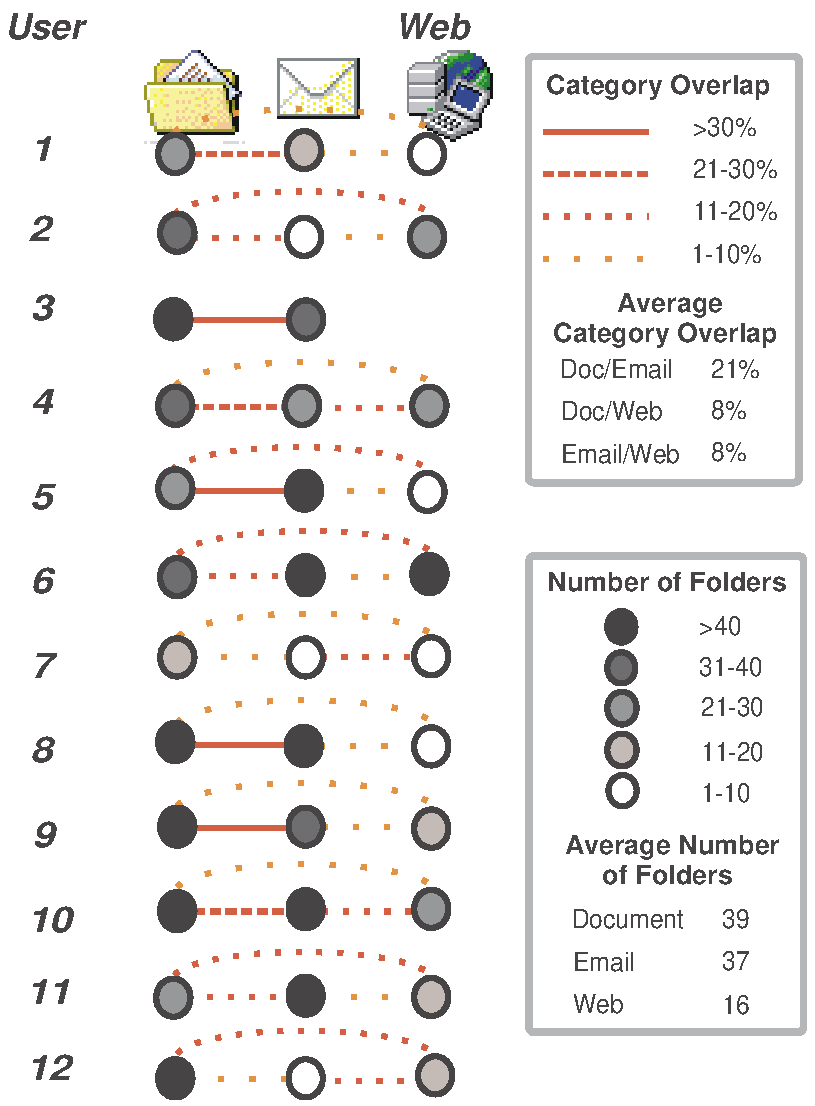
\includegraphics{pictures/exp-study/exp-study-OverlapResults.pdf}
%	\end{center}
%	\caption{Folder Overlaps for individual users [n=12]}
%	\label{fig:exp-study:overlaps-per-user}
%\end{figure}
Significant overlap was observed for many participants, particularly between files and email.   
For the twenty-two participants who had both file and email folders, the average \textit{file/email} overlap was 7.4 folders (SD: 4.6, min: 0, max: 21).
The other overlaps were consistently smaller.  For the eighteen participants with file and bookmark folders, the average \textit{file/bookmark} overlap was 2.6 folders (SD: 1.94, min: 0, max: 8).  Eighteen participants had created email and bookmark folders. The average \textit{email/bookmark} overlap was 2.0 folders (SD: 1.5, min: 0, max: 5).
% The file/web and email/web overlaps were on average almost three times smaller.
In other words, folder overlap was not distributed evenly between the hierarchy pairs\footnote{Overlaps were lower than previously estimated in~\citep{rpb:01a}. This is due to the earlier results being skewed upwards by the smaller number of subjects at that stage in the study.}.

%%%%%%%%%%%%%%%%%%%%%%%%%%%%%%%%%%%%%%%%%%%%%%%%%%%%%%
% TABLE: FOLDER OVERLAPS
% in tables/ch2/exp-study-tables.xls
%%%%%%%%%%%%%%%%%%%%%%%%%%%%%%%%%%%%%%%%%%%%%%%%%%%%%%
\begin{table}[hbp]
\begin{center}
\begin{footnotesize}
\setlength{\extrarowheight}{2pt}
\begin{tabular}{|p{4cm}|p{3cm}|p{3cm}|p{3cm}|}
% Table generated by Excel2LaTeX from sheet 'Folder Overlaps'
\hline
    {\bf } & {\bf File/email} & {\bf File/web} & {\bf Email/web} \\
\hline
{\bf \# participants with folders in corresponding tools} &         22 &         18 &         18 \\
\hline
{\bf Average overlap (\# of folders)} & 7.4 (SD: 4.6, min: 0, max: 21) & 2.6 (SD: 1.94, min: 0, max: 8) & 2.0 (SD: 1.5, min: 0, max: 5) \\
\hline
{\bf Average overlap as \% of file folders} & 16.3\% (SD:12.2\%, min: 0\%, max: 46.4\%) & 6.6\% (SD:5.4\%, min:0\%, max: 22.2\%) &        n/a \\
\hline
{\bf Average overlap as \% of email folders} & 21.6\% (SD:11.8\%, min:0\%, max: 40\%) &        n/a & 9.6\% (SD:10\%, min:0\%, max: 33\%) \\
\hline
{\bf Average overlap as \% of bookmark folders} &        n/a & 24.7\% (SD:17.2\%, min:0\%, max: 66.7\%) & 17.3\% (SD:12.4\%, min:0\%, max: 40\%) \\
\hline
\end{tabular}  
\end{footnotesize}
\caption{Folder overlaps between the three pairs of PIM-tools}
\label{table:category-overlaps}
\end{center}
\end{table}


Interestingly, as in the case of P19 above, the \textit{file/bookmark} and \textit{email/bookmark} overlaps tended to be a subset of the larger \textit{file/email} overlap. For the majority of subjects, the two smaller overlaps were almost identical. In other words, the subset they represented was common to all three tools.
%%%%%%%%%%%%%%%%%%%%%%%%%%%%%%%%%%%%%%%%%%%%
% EMPHASISE OVERLAP BETWEEN ALL 3 TOOLS
%%%%%%%%%%%%%%%%%%%%%%%%%%%%%%%%%%%%%%%%%%%%


%%%%%%%%%%%%%%%%%%%%%%%%%%%%%%%%%%%%%%%%%%%%%%
% Dimensional make-up of overlapping folders
%%%%%%%%%%%%%%%%%%%%%%%%%%%%%%%%%%%%%%%%%%%%%%
% Most overlapping folders were based on users' projects (40\%) or roles (27\%).
% RATIONALE: The purpose of this analysis was to see if overlapping folders tended to be based on a particular organizational dimensions . 
\textbf{Tables~\ref{table:file-email-overlap}}, \textbf{\ref{table:file-bookmark-overlap}}, and \textbf{\ref{table:email-bookmark-overlap}} show the organisational dimensions for the overlapping folders in each collection pair.  Interestingly, all three overlaps were predominantly based on the users' \textit{roles} and \textit{projects} (file/email: 75\%, file/bookmark: 79\%, email/bookmark: 79\%). This suggests that the dimensions of \textit{role} and \textit{project} are more likely to carry meaningful context across an entire workspace than other types of label. % Such overlap suggests that multiple types of information are involved in high-level user roles and activities.

%%%%%%%%%%%%%%%%%%%%%%%%%%%%%%%%%%%%%%%%%%%%%%%%%%%%%%
% TABLE: DIMENSIONS IN FILE/EMAIL OVERLAP (GROUP C USERS)
% in tables/ch2/exp-study-tables.xls
%%%%%%%%%%%%%%%%%%%%%%%%%%%%%%%%%%%%%%%%%%%%%%%%%%%%%%
\begin{table}[hbt]
\begin{center}
\begin{footnotesize}
\setlength{\extrarowheight}{2pt}
% Table generated by Excel2LaTeX from sheet 'File-EM O-Dims'
\begin{tabular}{|c|c|c|c|}
\hline
{\bf Rank} & {\bf Dimension in file/email folder overlap} & {\bf Count} &   {\bf \%} \\
\hline
   {\bf 1} &    Project &         60 &       36\% \\
\hline
   {\bf 2} &       Role &         59 &       36\% \\
\hline
   {\bf 3} &    Contact &         14 &        8\% \\
\hline
   {\bf 4} & Topic / interest &         13 &        8\% \\
\hline
   {\bf 5} & Document class &          5 &        3\% \\
\hline
   {\bf 6} &     Format &          5 &        3\% \\
\hline
   {\bf 7} &      Event &          4 &        2\% \\
\hline
   {\bf 8} &    General &          3 &        2\% \\
\hline
   {\bf 9} & Other (<3 folders) &          3 &        2\% \\
\hline
           & {\bf Total} &  {\bf 166} & {\bf 100\%} \\
\hline
\end{tabular}  
\end{footnotesize}
\caption{Organisational dimensions in file/email folder overlap [n=22]}
\label{table:file-email-overlap}
\end{center}
\end{table}

%%%%%%%%%%%%%%%%%%%%%%%%%%%%%%%%%%%%%%%%%%%%%%%%%%%%%%%
% TABLE: DIMENSIONS IN FILE/BOOKMARK OVERLAP (GROUP C USERS)
% in tables/ch2/exp-study-tables.xls
%%%%%%%%%%%%%%%%%%%%%%%%%%%%%%%%%%%%%%%%%%%%%%%%%%%%%%%
\begin{table}[hbt]
\begin{center}
\begin{footnotesize}
\setlength{\extrarowheight}{2pt}
% Table generated by Excel2LaTeX from sheet 'File-BM O-Dims'
\begin{tabular}{|c|c|c|c|}
\hline
{\bf Rank} & {\bf Dimension in file/bookmark folder overlap} & {\bf Count} &   {\bf \%} \\
\hline
   {\bf 1} &    Project &         17 &       41\% \\
\hline
   {\bf 2} &       Role &         11 &       27\% \\
\hline
   {\bf 3} & Topic / interest &          9 &       22\% \\
\hline
   {\bf 4} &    Contact &          2 &        5\% \\
\hline
   {\bf 5} & Other (<2 folders) &          2 &        5\% \\
\hline
    {\bf } &     {\bf Total} &   {\bf 41} & {\bf 100\%} \\
\hline
\end{tabular}  
\end{footnotesize}
\caption{Organisational dimensions in file/bookmark folder overlap [n=18]}
\label{table:file-bookmark-overlap}
\end{center}
\end{table}

%%%%%%%%%%%%%%%%%%%%%%%%%%%%%%%%%%%%%%%%%%%%%%%%%%%%%%%
% TABLE: DIMENSIONS IN EMAIL/BOOKMARK OVERLAP (GROUP C USERS)
% in tables/ch2/exp-study-tables.xls
%%%%%%%%%%%%%%%%%%%%%%%%%%%%%%%%%%%%%%%%%%%%%%%%%%%%%%%
\begin{table}[hbt]
\begin{center}
\begin{footnotesize}
% Table generated by Excel2LaTeX from sheet 'EM-BM O-Dims'
\begin{tabular}{|c|c|c|c|}
\hline
{\bf Rank} & {\bf Dimension in email/bookmark folder overlap} & {\bf Count} &   {\bf \%} \\
\hline
  {\bf 1=} &    Project &         11 &       35\% \\
\hline
  {\bf 1=} &       Role &         11 &       35\% \\
\hline
   {\bf 2} & Topic/interest &          5 &       16\% \\
\hline
   {\bf 3} & Document class &          2 &        6\% \\
\hline
   {\bf 4} & Other (<2 folders) &          2 &        6\% \\
\hline
    {\bf } & {\bf Total} &   {\bf 31} & {\bf 100\%} \\
\hline
\end{tabular}  

\end{footnotesize}
\caption{Organisational dimensions in email/bookmark folder overlap [n=18]}
\label{table:email-bookmark-overlap}
\end{center}
\end{table}


%%%%%%%%%%%%%%%%%%%%
\subsection{Discussion}
\label{exp-study:Results-folder-overlap-discussion}
%%%%%%%%%%%%%%%%%%%%
%%%%%%%%%%%%%%%%%%%%%%%%%%%%%%%%%%%%%%%%%%%%%%%%%%%%%%%%%%%%
% TO ADD: WHY WAS THIS DONE? WHAT IS THE MAIN CONCLUSION?
%%%%%%%%%%%%%%%%%%%%%%%%%%%%%%%%%%%%%%%%%%%%%%%%%%%%%%%%%%%%

%%%%%%%%%%%%%%%%%%%%%%%%%%%%%%%%%%%
% Highest between files and email
%%%%%%%%%%%%%%%%%%%%%%%%%%%%%%%%%%%

%%%%%%%%%%%%%%%%%%%%%%%%%%%%%%%%%%%%%%%%%%%%%%%%%%%%%%%%%%%%%%%%
% Provide examples of overlap
% Provide examples of non-overlap (tool-specific activities)
%%%%%%%%%%%%%%%%%%%%%%%%%%%%%%%%%%%%%%%%%%%%%%%%%%%%%%%%%%%%%%%%
% \textit{Provide examples of overlapping folders (cross-tool activity) and tool-specific activities. }
The observation of a significant partial folder overlap for most participants points to a subset of user activities that involve the management of multiple types of information.  Folder overlap indicates that the study participants were devoting effort towards organizing resources relating to the same production activity in multiple tools.  In other words, there are \textit{redundant} aspects to user's information management activity when viewed from a cross-tool perspective.  Most overlapping folders corresponded to \textit{roles} and \textit{projects}, suggesting that these concepts may be usefully shared between collections, as in~\citep{Kaptelinin:03}.

However, it should be emphasized that folder overlap was only partial: all collections contained many unique folders.  This suggests that: (1) some production tasks are supported by single PIM tools and may not necessarily benefit from increased integration; and (2) users may have different organizational needs in different tools. 
% what does it mean in the grand scale of things? Provide balanced view a la Andrew Monk}.
% PIM-support for particular production activities is distributed across multiple PIM-related tools
% Distributed in time? Inter-tool consistency
%%%%%%%%%%%%%%%%%%%%%%%%%%%
% Reasons for overlap
% Reasons for no overlap
%%%%%%%%%%%%%%%%%%%%%%%%%%%
Several factors may contribute towards the disparity in overlap between different pairs of tools.

\begin{itemize}

\item Firstly, the number of folders differed greatly between the tools.  Typically bookmark collections contained fewer folders, resulting in smaller overlaps. In general bookmark organisation was not seen as being of as high a priority as file and email organisation, with subjects often preferring to use search engines in preference to recording bookmarks.

\item The previous section outlined the organisational make-up of each hierarchy and it was noted that the file and email hierarchies were relatively similar, both being dominated by \textit{projects} and \textit{roles}. This may account for their higher overlap. In contrast, the majority of bookmark labels were based on  \textit{interests} that had little relevance outside the information-seeking context of the web.

\item Document and email folders also tended to be managed more consistently in an ongoing manner -- thus the folders might be expected to match to a greater extent.

\item The information stored in each hierarchy may also be a factor. The file system was used to manage the user's own documents, or those authored by colleagues or friends. Likewise the email folders were often used to store threads of communication in which the user had actively participated (the storing of mailing lists is an exception). Both the document and email folders convey ownership over the static resources archived within. On the other hand, bookmark folders are used to store references to remotely authored websites. 

\end{itemize}

%%%%%%%%%%%%%%%%%%%%%%%%
% Awareness of overlap
%%%%%%%%%%%%%%%%%%%%%%%%
Most participants were not aware of the often significantly high level of overlap between their hierarchies.  Some participants seemed surprised when their high level of folder overlap was pointed out, suggesting that they had not reflected on how they organized different types of information.  A few were more aware and actually performed ad-hoc synchronisation of organisational structure. One participant (P11) had spent a large amount of time synchronising her email and web hierarchies. However the amount of effort involved meant the structures had not been kept in full synchronization.
% ADD: sample of anecdotal observations   regarding folder overlap and what it might mean(pos: dmw, neg: mar)

%%%%%%%%%%%%%%%%%%%%%%%%%
% DESIGN IMPLICATIONS
%%%%%%%%%%%%%%%%%%%%%%%%%
Folder overlap was greatest between the file and email collections. This highlights the potential compatibility for integration of files and \textit{filed} email. Also both types of information are either self-created or assessed as having long-term value.  However complete unification between files and \textit{all} email (as pointed to by designs such as~\citep{Bellotti:03}) may lead to the disruption of more controlled items (e.g. files, tasks) by unprocessed email. In some cases it may be appropriate not to integrate, but to instead retain tool separation.  Further design implications are presented in \textbf{Section~\ref{exp-study:discussion:integration}}.

%%%%%%%%%%%%%%%%%%%%%%%%%%%%%%
% hint at WorkspaceMirror?
%%%%%%%%%%%%%%%%%%%%%%%%%%%%%%
The observation of folder overlap contributes to the design rationale for the development of the WorkspaceMirror prototype in \textbf{Chapter~\ref{chapter:design}}. % Evidence is also provided of the cross-tool nature of information management: as an activity that supports a user's production activities.

%%%%%%%%%%%%%%%%%%%%%%%%%%%%%%%%%%%%%%%%%%%
%% END RESULTS2-FOLDER-OVERLAP/CHAPTER 4 EXP STUDY
%%%%%%%%%%%%%%%%%%%%%%%%%%%%%%%%%%%%%%%%%%%


 

%%%%%%%%%%%%%%%%%%%%%%%%%%%%%%%%%%%%%%%%%%%%%%%%%%%
\newpage
\section{Results: Changes in Organizing Strategy}
\label{exp-study:comparison-changes}
%%%%%%%%%%%%%%%%%%%%%%%%%%%%%%%%%%%%%%%%%%%%%%%%%%%
% Immediate, Planned, Historical


%%%%%%%%%%%%%%%%%%%%%
% IMMEDIATE
%%%%%%%%%%%%%%%%%%%%%
The study had an immediate ``self-auditing'' influence on the behaviour of most participants.
Many participants rediscovered items they had lost, and twelve performed ad-hoc tidying during the interviews, e.g. filing or deleting files they had forgotten about.
% Self-audit: rediscover info, duplicated, failed, misfiled, tofile, old, todelete, useful 

% Changes included ones made during the studies, planned

%%%%%%%%%%%%%%%%%%%%%
% FILES
%%%%%%%%%%%%%%%%%%%%%
Fourteen participants reported historical strategy changes from before the study. Five reported historical changes in file strategy, all of which involved increases in organization, e.g. P5: \textit{``Now I've got a set of folders and create a new one if I've got too many unfiled.  Historically I use to be less organized and everything was unfiled.  I still have to search for this using type or date metadata''}.

%%%%%%%%%%%%%%%%%%%%%
% EMAIL
%%%%%%%%%%%%%%%%%%%%%
In email, seven participants reported historical changes in organizing strategy  -- three increases and four decreases in filing tendency.  Several participants also reported major incidents, such as a hard disk failure which lead to the loss of an email collection.  One example decrease in organizing tendency was as follows, e.g. P12: \textit{``I used to have lots of folders for each sub-project [of a main research area] but there just wasn't enough time to manage them. In an ideal world there'd be a rich structure ... and the hierarchy is now flattened and simplified''}.

%%%%%%%%%%%%%%%%%%%%%
% BM
%%%%%%%%%%%%%%%%%%%%%
In the case of bookmarks, six historical changes were reported: one increase, and five decreases in organization (e.g. abandoning all folders).

%%%%%%%%%%%%%%%%%%%%%%%%%%
\subsection{Discussion}
%%%%%%%%%%%%%%%%%%%%%%%%%%

%%%%%%%%%%%%%%%%%%%%%
% BOTH INC AND DEC
%%%%%%%%%%%%%%%%%%%%%
Note that both increases and decreases in organizing tendency were observed. This stands in contrast to previous work which has emphasized decreases in organizing tendency, e.g. the abandoning of folder structures~\citep{ob:97}. 

%%%%%%%%%%%%%%%%%%%%
% MAJOR INCIDENTS
%%%%%%%%%%%%%%%%%%%%
% However participants were typically settled in their choice of management strategy	

Additionally, many indicated that taking part in the study had caused them to think about PIM more than normal, causing them to plan future changes.  However, the snapshot nature of the nature meant that it was not possible to track these changes over time.
%%%%%%%%%%%%%%%%%%%%%%%%%%%%%%%%%%%%%%%%%%%%%%%%%%%%%%%%%%%%
% LINK TO CAHPTER 6
%%%%%%%%%%%%%%%%%%%%%%%%%%%%%%%%%%%%%%%%%%%%%%%%%%%%%%%%%%%%
\textbf{Chapter~\ref{chapter:main-study}} presents a longitudinal study of PIM behaviour, a key objective of which was to track strategy changes. 

% This exploratory study provided the incentive to investigate such issues in more depth. 

%%%%%%%%%%%%%%%%%%%%%%%%%%%%%%%
% CHAPTER 4: EXPLORATORY STUDY
% RESULTS 5 - Results: Problems and User Experience
% File: tex/expstudy-chapter/expstudy-results7-problems.tex
%%%%%%%%%%%%%%%%%%%%%%%%%%%%%%%%%%%%%%%%%%%%%%%%
%%%%%%%%%%%%%%%%%%%%%%%%%%%%%%%%%%%%%%%%%%%%%%%%
%%%%%%%%%%%%%%%%%%%%%%%%%%%%%%%%%%%%%%%%%%%%%%%%
%%%%%%%%%%%%%%%%%%%%%%%%%%%%%%%%%%%%%%%%%%%%%%%%%%%%
\newpage
%%%%%%%%%%%%%%%%%%%%%%%%%%%%%%%%%%%%%%%%%%%%%%%%%%%
\section{Results: Problems and User Experience}
\label{exp-study:comparison-problems}
%%%%%%%%%%%%%%%%%%%%%%%%%%%%%%%%%%%%%%%%%%%%%%%%%%%
% NOTES
% * take care not to exaggerate problems
%	* Integrate discussion points (nature of PIM, e.g. reflection/distribution) into here??
%%%%%%%%%%%%%%%%%%%%%%%%%%%%%%%%%%%%%%%%%%%%%%
% ALT STRUCTURE: Key problems in different aspects of PIM
%%%%%%%%%%%%%%%%%%%%%%%%%%%%%%%%%%%%%%%%%%%%%%
% grievances
% the most fundamental/common points raised.  However note that problems varied across participants. %% EXPAND THIS - say everyone mentioned a different problem (for some version control was the bugbear, for others it was naming files
The study provided much evidence of dissatisfaction regarding current PIM interfaces.  
The author was often surprised at the vehemence expressed regarding PIM-related problems, and applied the term ``bugbear'' for recurring problems that frequently affected users.  Since PIM is an ongoing and often repetitive everyday activity, it appeared that even relatively minor short-term grumbles (e.g. inconvenient interface support for naming files) can build up and have a negative impact on ongoing user experience (e.g. perceived level of control).  
% \textit{Aim of design: to improve user experience.  FOCUS: INTEGRATION.  Argue need for more cross-tool design of integration-mechanisms.}

%%%%%%%%%%%%%%%%%%%%%%%%%%%
% Lead onto Cross-tool problems
%%%%%%%%%%%%%%%%%%%%%%%%%%%
%any problems are cross-tool, or at least compounded. \textit{THINK: Mention bugbears?}
% Potential of mismapping betwen activities and tools
% Problems at various contexts: (1) within specific tools (intra-tool problems), (2) the same problem in multiple tools, and (3) problems that bridged multiple tools. This third time of problem is discussed in \textbf{Section~\ref{exp-study:comparison-cross-tool}}.
% The discussion up until now has focused on user problems within particular PIM tools. WE also observed a range of \textit{cross-tool} problems, problems that bridged multiple collections 
A wide range of problems and concerns were raised by participants relating to all PIM sub-activities in all three PIM-tools.  Furthermore, issues varied significantly between participants.  This section highlights some of the issues that are relevant to subsequent work in this thesis.  Three types of problem were identified:
\begin{enumerate}
\item Tool-specific issues that were limited to single tool contexts.
% Tool-specific problems that occurred in multiple tool contexts 
\item Tool-specific issues that occurred repeatedly in multiple distinct tool contexts.
\item Cross-tool issues that bridged multiple tool contexts. 
\end{enumerate}

%%%%%%%%%%%%%%%%%%%%%%%%%%%%%%%%%%%%%%%
\subsection{Tool-specific Issues}
\label{exp-study:tool-specific}
%%%%%%%%%%%%%%%%%%%%%%%%%%%%%%%%%%%%%%%
% Problems that were limited to single tools (tool-specific issues)
%	\item Mention a few of the extreme/far-out examples/outliers of problems (e.g. version control esp docs/email)
%	Acquisition-related problems were focused on inbox management in email. Many participants complained of the time they spent processing messages and deciding which to keep.  
Numerous PIM-problems were reported within each tool collection.  File-related problems included difficulties managing multiple versions of files, and slow search mechanisms.  A key email-related problem was that of ascertaining the value of large numbers of newly-arrived messages.  Common issues in the bookmark context included lack of sorting and search functionality, and the ephemeral nature of websites.

% This section, and subsequent chapters of the thesis focus on problems that 
Since the thesis takes a focus on problems that bridge multiple tools, tool-specific problems are not discussed in more detail.

%%%%%%%%%%%%%%%%%%%%%%%%%%%%%%%%%%%%%%%%%%%%%%%%%%%%%%%%%%%%%%%%%%%%%%%%%%%%%%%%%%%%%%%%%%%%%%%%
%%%%%%%%%%%%%%%%%%%%%%%%%%%%%%%%%%%%%%%%%%%%%%%%%%%%%%%%%%%%%%%%%%%%%%%%%%%%%%%%%%%%%%%%%%%%%%%%
%%%%%%%%%%%%%%%%%%%%%%%%%%%%%%%%%%%%%%%%%%%%%%%%%%%%%%%%%%%%%%%%%%%%%%%%%%%%%%%%%%%%%%%%%%%%%%%%
%%%%%%%%%%%%%%%%%%%%%%%%%%%%%%%%%%%%%%%%%%%%%%%%%%%%%%%%%%%%%%%%%%%%%%%%%%%%%%%%%%%%%%%%%%%%%%%%

%%%%%%%%%%%%%%%%%%%%%%%%%%%%%%%%%%%%%%%%%%%%%%%%%%%%%%%%%%%%%%%%%%%%%%%%%%%%%%
\subsection{Tool-specific Issues that Occurred in Multiple Tools}
\label{exp-study:issues-repeated}
%%%%%%%%%%%%%%%%%%%%%%%%%%%%%%%%%%%%%%%%%%%%%%%%%%%%%%%%%%%%%%%%%%%%%%%%%%%%%%

Other problems were of a tool-specific nature, and were manifested in multiple contexts for many participants.  Examples included difficulties in naming items, and ``anxiety of order''.

%%%%%%%%%%%%%%%%%%%%%%%%%%%%%%%%%%%%%%%%%%%%%
% MULTI-CONTEXT PROBS: ACQUISITION/NAMING
%%%%%%%%%%%%%%%%%%%%%%%%%%%%%%%%%%%%%%%%%%%%%
% ACQUISITION/NAMING: Other acquisition-related problems included being forced to name items in the file system, and poor default naming for bookmarks. Also hard to rename emails.
One common problem that appeared in multiple tool contexts related to the naming of items.  Participants complained of the difficulty of selecting appropriate, meaningful names in their file collections.  One particular bugbear resulted from the attempts of software to offer default names based on a file's initial content (e.g. a report title).  In email, many participants complained of the difficulty in changing message subjects.  Those created by other users were often considered inadequate.  Likewise, in bookmarks participants complained of the poor interface provision for changing the names of newly-created bookmarks.  This was often necessary as by default bookmark names are set to the title of a web page to which they refer.  Several participants observed that web page names were often general to entire web-sites.

%%%%%%%%%%%%%%%%%%%%%%%%%%%%%%%%%%%%%%%%%%%%%
% MULTI-CONTEXT PROBS: ANXIETY OF ORDER
%%%%%%%%%%%%%%%%%%%%%%%%%%%%%%%%%%%%%%%%%%%%%
% ANXIETY OF ORDER: The most common observed organization-related problem was \textit{anxiety of order} e.g. old/failed/duplicate folders, unfiled items
% Many \textit{pro-organizing} participants suffered from an ``anxiety of order''~\citep{levy:01}.
% Classic tree problems (multiple classification, static hierarchy) rarely mentioned (COUNT USERS). Some (failed folders, duplicate folders) mentioned in context of staying tidy 
% What can WE conclude from this.  Users satisfice -- therefore no need for multiple attributes?  
% Postulate: some people have a disposition to keep things tidy.  
Another problem that appeared in multiple tool contexts was that of ``anxiety of order''~\citep{levy:01}.  This describes the tendency for many users to ``feel bad'' for ``being untidy''.  In other words, a perceived failure to manage personal information may seriously dent user's self-image.

Anxiety of order was widespread in the study reported in this chapter.  Many participants felt it necessary to excuse themselves for perceived mess, e.g. Participant P21: \textit{``I'm sorry, those files must have gone there accidently''}.  Anxiety was most extreme in the context of email, where participants emphasized the overheads of managing email, due to the higher (and uncontrolled) creation rate of messages compared to manually created files and bookmarks. % laso exacerbated by spam!).
However, participants also tended to be dissatisfied with the organizational state of document files and bookmarks, especially in terms of old or unfiled items, and failed folders. Dissatisfaction was expressed in terms of guilt, shame, stress, and lack of control, P11: \textit{``I'm really ashamed ... Its such a mess! I have stuff in there that needed organizing ages ago''}.

% Most participants said that they did not have enough time to organize the collections, resulting in a lack of satisfaction regarding their tidiness.  
A particular source of exasperation was the existence of old unfiled items, such as emails in the inbox, and icons on the desktop. Most participants wanted to devote more time to managing their personal information but could not do so due to lack of time or were unwilling to do so because of perceived overheads.

The level of anxiety was influenced by user disposition towards tidiness, with organizing-neutral participants being less affected.  Interestingly, some of the most pro-organizing participants, those who invested a lot of time in filing, remained dissatisfied with the tidiness of their collections. 

Anxiety of order was possibly exacerbated by other ``classic'' classification problems which were reported in all tool contexts by many participants.  These included difficulties classifying items, lack of multiple classification support, failed folders, duplicate folders, and the static nature of the folder hierarchy.  The increasing amount of storage in modern computing devices may be a contributory factor in user dissatisfaction: since (1) they are able to collect more stuff, and (2) there is less pressure to delete information in an ongoing manner.

Only a few participants complained of the impact on their productivity due to time spent organizing, and time spent retrieving items.  However this is subjective and hard to confirm objectively.  Impact of messiness is not clear on retrieval since participants indicated that they could generally find required items. 

% Maintenance problems were rarely mentioned by participants except for the fact that they had little time for archiving etc. Another maintenance-related problem was expressed in terms of not maintaining, e.g. when participants had failed to back-up.

%%%%%%%%%%%%%%%%%%%%%%%%%%%%%%%%%%%%%%%%%%%%%%%%%%%%%%%%%%%%%%%%%%%%%%%%%%%%%%%%%%%%%%%%%%%%%%%%
%%%%%%%%%%%%%%%%%%%%%%%%%%%%%%%%%%%%%%%%%%%%%%%%%%%%%%%%%%%%%%%%%%%%%%%%%%%%%%%%%%%%%%%%%%%%%%%%
%%%%%%%%%%%%%%%%%%%%%%%%%%%%%%%%%%%%%%%%%%%%%%%%%%%%%%%%%%%%%%%%%%%%%%%%%%%%%%%%%%%%%%%%%%%%%%%%
%%%%%%%%%%%%%%%%%%%%%%%%%%%%%%%%%%%%%%%%%%%%%%%%%%%%%%%%%%%%%%%%%%%%%%%%%%%%%%%%%%%%%%%%%%%%%%%%



%%%%%%%%%%%%%%%%%%%%%%%%%%%%%%%%%%%%%%%%%%%%%%%%
\subsection{Issues that Bridged Multiple Tools}
\label{exp-study:issues-cross-tool}
%%%%%%%%%%%%%%%%%%%%%%%%%%%%%%%%%%%%%%%%%%%%%%%%
% Include stuff from CSCW2002 paper
% * Need to relate to conceptual framework of tools and activities in Chapter 1
%	* make sure production/supporting activity are defined
%	* Cross-tool problems as basis for scenarios in next chapter
%%%%%%%%%%%%%%%%%%%%%%%%%%%%%%%%%%%%%%%%%%%%%%%%

A number of problems were observed that bridged multiple tool contexts:
\begin{enumerate}
\item Design inconsistencies between different PIM-tools.
\item The inability to share folder structures between PIM-tools.
\item The fragmentation across PIM-tools of information in a particular technological format.
\item The fragmentation of information related to a particular activity across PIM-tools.
\end{enumerate}

%%%%%%%%%%%%%%%%%%%%%%%%
% INCONSISTENCIES
%%%%%%%%%%%%%%%%%%%%%%%%
% Example functionality which was implemented differently included ``create new folder'' or ``mark this item as important''
% Inconsistencies, interface inconsistency. % Reference to previous work on consistency (\textit{standard result in HCI?})
Annoyance was caused by inconsistencies between different PIM-tools in terms of how they provided equivalent functionality.  One example was the interface used to manipulate the folder structure by changing folder names, or reorganizing the folder structure.  Participants found this particularly irritating between tools from the same vendor.  In other cases, a function was available in one tool, but not in others.  One example was the ability to highlight an item as ``important''.  Email clients such as MS-Outlook provide the ability to ``flag'' an item, whereas file and web bookmark management software typically does not.

%%%%%%%%%%%%%%%%%%%%%%%%%%%
% COMPOUNDED OVERHEADS
%%%%%%%%%%%%%%%%%%%%%%%%%%%
% Evidence that magnify and compound above basic PIM problems. Overhead. Overload. Talk about in terms of forced-split attention, parallel working. Extent to which some users avoid separate management. % \textit{QUOTE: gil?} 
Several participants complained of the need to manage different collections of information separately, noting that it was not possible to share organizational structure between tools.  One went to the lengths of saving email messages as files to avoid having to manage two distinct collections.  When viewed from a cross-tool perspective it is clear that the management overheads that have been reported in specific tools are compounded when multiple PIM tools are considered.

%%%%%%%%%%%%%%%%%%%%%%%%%%%%%%%%%%%%%%%%%%%%%%%%%%%%%%%%%%%%%%%%%%%%%%%%%%
% FRAGMENTATION: OF SPECIFIC TECH FORMATS
% The fragmentation of information of a particular technological format.
%%%%%%%%%%%%%%%%%%%%%%%%%%%%%%%%%%%%%%%%%%%%%%%%%%%%%%%%%%%%%%%%%%%%%%%%%%
% Despite the presence of compartmentalization, users tended to focus their PIM efforts on a \textit{primary collection} (MOVE TO LATER)
Participants also complained that information in some technological formats was fragmented across multiple distinct collections.  For instance, many participants managed files using several parallel mechanisms: (1) within the file system, (2) spatially as desktop icons, and (3) as email attachments. Each mechanism requires separate organization.  This distribution of the management of a particular type of information between distinct PIM-tools has been referred to as \textit{compartmentalization}~\citep{Bellotti:00}.  \textbf{Table~\ref{table:compartmentalization}} summarizes the observations of the compartmentalization of document files, email, and web bookmarks -- both within a single computer, and across the extended personal information environment\footnote{Compartmentalization was also observed for other types of personal information such as contacts and to-do items.  For example, contacts were frequently scattered between email, personal diaries, notebooks, and mobile phones.}.
%%%%%%%%%%%%%%
% RETRIEVAL
%%%%%%%%%%%%%%
Several participants reported that the compartmentalization of files lead to problems of retrieval, especially in the case that they were looking for a particular file and had to search both the file and email collections.% Issues and problems relating to the compartmentalization of document files, email and web bookmarks is discussed in more detail in \textbf{Section~\ref{exp-study:ct}}
% Consequences for version control
%%%%%%%%%%%%%%%%%%%%%%%%%%%%%%%%%%%%%%%%%%%%%
% MULTI-CONTEXT PROBS: RETRIEVAL
%%%%%%%%%%%%%%%%%%%%%%%%%%%%%%%%%%%%%%%%%%%%%
% RETRIEVAL: participants mentioned encountering only occasional problems, although these were highly frustrating. In contrast failure to find things was mentioned less often. % See \textbf{Section~\ref{exp-study:comparison-retrieval}}.

\begin{table}[hbtp]
\begin{center}
\begin{footnotesize}
\setlength{\extrarowheight}{2pt}
\begin{tabular}{|p{2.5cm}|p{3.5cm}|p{3.5cm}|p{3.5cm}|}
\hline
 & {\bf Document File} & {\bf Email} & {\bf Web Bookmark} \\
\hline
{\bf On primary computer} & Document files can also be managed as desktop icons or as email attachments.  & Email typically managed only within email tool. & Web bookmarks often managed as desktop icons or as embedded links within emails.  \\
\hline
{\bf Outside primary desktop computer} & Network drives. Personal document files stored on other computers or devices. & Email stored on other computers or devices. Web-email collections (such as Yahoo! or Hotmail) & Web bookmarks stored on other computers or devices.  \\
\hline
\end{tabular}  
\end{footnotesize}
\caption{Compartmentalization of different types of information}
\label{table:compartmentalization}
\end{center}
\end{table}
\normalsize

%%%%%%%%%%%%%%%%%%%%%%%%%%%%%%%%%%%%%%%%%%%%%%%%%%%%%%%%%%%%%%%%%%%%%%%%%%
% FRAGMENTATION: INFO RELATED TO ONE ACTIVITY
%%%%%%%%%%%%%%%%%%%%%%%%%%%%%%%%%%%%%%%%%%%%%%%%%%%%%%%%%%%%%%%%%%%%%%%%%%
% The fragmentation of information relating to a particular activity.	
% Users complained about the need to coordinate production activities across multiple tools. 
% Several participants mentioned activities which involved PIM-tools.  
Another aspect of fragmentation concerned information relating to a particular user activity such as a project.  A number of participants highlighted difficulties in coordinating multiple PIM-tools in carrying out a particular project.
%  such as starting a project, or finishing a project
One difficulty was encountered in \textit{project management}-related tasks such as starting a new production activity (setting up folders in distinct tools), and finishing a production activity (archiving items in distinct tools).  One participant talked of the difficulties involved in archiving two types of information, P1: \textit{``After the project finished it was all 99\% useless stuff [files and email]. I just wanted to get it out of the way''}. In such cases, it was necessary to perform these actions repeatedly in multiple tools.  This type of fragmentation also impacted retrieval, when a user is not sure if the information related to an activity is stored in an email or a file.

%%%%%%%%%%%%%%%%%%%
% BRAINSTROMING
%%%%%%%%%%%%%%%%%%%
% Add collating examples: idea brainstorming, gathering ideas. % Ad-hoc categories (SJ)
Some participants wanted a facility to gather different types of information within a single interface. One example was \textit{brainstorming} which involved collating information from multiple PIM-tools into her email, P9: \textit{``I like to pull things together here, URLs, notes ... and jumble them up in broad categories. My categories tend to be fairly wide and get quite big.  It's great for brainstorming and ideas. However the cost is that sometimes you can't find things''}.

%%%%%%%%%%%%%%%%%%%%%%%%
% REMINDERS
%%%%%%%%%%%%%%%%%%%%%%%%
% The author speculates that the users have problems staying on top of all these reminders.
% Cross-tool aspects of PIM, Aspects of PIM such as information management and task management can be considered as cross-tool: they cut across a wide range of tools. 
Most participants employed a range of PIM-tools in performing task and time management, e.g. setting reminders in multiple tool contexts such as icons on the desktop, emails in the inbox, and links to websites to visit. Most also made extensive use of physical artefacts such as diaries.  Two participants complained that there was no easy way to collate such reminders together.

%%%%%%%%%%%%%%%%%%%%%%%%%%%%%%%%%%%%%%%%
% Usage of existing forms of integration
%%%%%%%%%%%%%%%%%%%%%%%%%%%%%%%%%%%%%%%%
Participants varied in the extent to which they reported using existing integration mechanisms.  The most commonly mentioned was attaching files to an message from within an email tool.  Several also mentioned using the ``Send-to'' mechanism in MS-Windows for attaching files to an email message.  % However note that current forms of integration fall short of solving the above problems and currently users have to coordinate manually across tools (e.g. gathering information of a particular technological format).

%%%%%%%%%%%%%%%%%%%%%%%%%%
\subsection{Discussion}
%%%%%%%%%%%%%%%%%%%%%%%%%%
%%%%%%%%%%%%%%%%%%%%%%%%%%%
% DISCUSSION AT THE END
%%%%%%%%%%%%%%%%%%%%%%%%%%%
% In this thesis, the author argues that PIM is a cross-tool activity, and should be designed for as such. This section discusses a number of findings that provided evidence to support the cross-tool perspective that is developed over the thesis: (1) the usage of existing forms of integration, and (2) problems that involved multiple tools. Such problems may indicate needs for improved integration. % Note that problems specific to particular tools are discussed in \textbf{Section~\ref{exp-study:comparison-problems}}.
The previous two sections illustrate a number of user problems that involve multiple PIM-tools. Firstly, \textbf{Section~\ref{exp-study:issues-repeated}} highlights \textit{tool-specific} problems which appeared in multiple tools.  Secondly, \textbf{\ref{exp-study:issues-cross-tool}} highlights a number of \textit{cross-tool} issues.  Such problems suggest that there is a need for improved integration between PIM-tools. \textbf{Chapter~\ref{chapter:design}} discusses prospective cross-tool design solutions to some of the problems discussed in this section.

% This thesis investigates how a cross-tool design perspective can be applied to solving such problems.  A number of potential solutions are outlined in \textbf{Chapter~\ref{chapter:design}}. 












	


 

%%%%%%%%%%%%%%%%%%%%%%%%%%%%%%%%%%%%%%%%%%%%%%%%%%%%%
% CHAPTER 4: EXPLORATORY STUDY
%%%%%%%%%%%%%%%%%%%%%%%%%%%%%%%%%%%%%%%%%%%%%%%%%%%%%
%% CONCLUSION
%%%%%%%%%%%%%%%%%%%%%%%%%%%%%%%%%%%%%%%%%%%%%%%%%%%%%
\newpage
\section{Discussion and Conclusion}
\label{exp-study:conclusion}
%%%%%%%%%%%%%%%%%%%%%%%%%%%%%%%%%%%%%%%%%%%%%%%%%%%%%
% EXTRAS FOR CONSIDERATION:
% EXTRA: nature of PIM - see towards a new conceptualization
%%%%%%%%%%%%%%%%%%%%%%%%%%%%%%%%%%%%%%%%%%%%%%%%%%%%%
% * 3 tools/3 ways of working
% * Contrasting user experience
%%%%%%%%%%%%%%%%%%%%%%%%%%%%%%%%%%%%%%%%%%%%%%%%%%%%%
% How to improving PIM experience
% * Most users get by ... are they really that bad?
% * change designs vs. change behaviour
% * Pros and cons of hierarchy. Relate to design rationale in \textbf{Chapter~\ref{chapter:design}}}
%%%%%%%%%%%%%%%%%%%%%%%%%%%%%%%%%%%%%%%%%%%%%%%%%%%%%
% Convergence of PIM tools and other trends
%	* email/bloggers being used to create documents
%	* same interface for multiple types of information (e.g. Windows explorer for docs and bm)
%	* but still sense of distinct collections
%	* Type of integration
%%%%%%%%%%%%%%%%%%%%%%%%%%%%%%%%%%%%%%%%%%%%%%%%%%%%%

%%%%%%%%%%%%%%%%%%%%%%%%
% Recap main findings
%%%%%%%%%%%%%%%%%%%%%%%%
% Recap and discuss substantive findings
% 1.Tool-specific and cross-tool insights
%		e.g. Problems
% 2.Individual differences
% 3.Comparison - Multiple PIM strategies
%		Intra-tool
%		Cross-tool profiling
% 4.Factors affecting PIM strategies
% 5.Conceptual basis
%		Change / time
%		Cross-tool (see below)
% 6.Cross-tool perspective
%		problems
%		activities
% 7.Implications for integration
%		Organizational dimensions
%		Folder Overlap (towards WM)
% 8.Methodological limitations
%	9.Conclusion
%		Moving on

%%%%%%%%%%%%%%%%%%%%%%%%%
% intro & structure
%%%%%%%%%%%%%%%%%%%%%%%%%
% Issues relating to the study methodology are also explored.
This section discusses the chapter's main findings, and relates them to the work presented in subsequent chapters.  Firstly, \textbf{Section~\ref{exp-study:discussion:indiv-diffs}} highlights methodological issues which should be taken into consideration when interpreting the study results. \textbf{Section~\ref{exp-study:discussion:multiple-strategies}} moves on to discuss the observation of multiple organizing strategies, within and across PIM-tools for many participants.  A model is presented to illustrate this new conceptualization of organizing strategies.
% Design implications following from the study findings are discussed. 
\textbf{Section~\ref{exp-study:discussion:integration}} considers implications for the design of PIM-integration technology based on the study findings.
% \textbf{Section~\ref{exp-study:discussion:conceptual-basis}} discusses three properties of PIM as an activity that is: (1) cross-tool, (2) supporting, and (3) ongoing/long-term.
Finally, \textbf{Section~\ref{exp-study:discussion:conclusion}} considers whether the study achieved the objectives in \textbf{Section~\ref{exp-study:introduction}}.



%%%%%%%%%%%%%%%%%%%%%%%%%%%%
% \subsection{Methodological limitations}
%%%%%%%%%%%%%%%%%%%%%%%%%%%%
%%%%%%%%%%%%%%%%%%%%%%%%%%%%%%%%%%%%%%%%%%%%%%%%%%%%%%%%%%%%%%%%%
\subsection{Methodological Limitations}
\label{exp-study:discussion:indiv-diffs}
%%%%%%%%%%%%%%%%%%%%%%%%%%%%%%%%%%%%%%%%%%%%%%%%%%%%%%%%%%%%%%%%%
% Idiosyncratic, individual differences
%%%%%%%%%%%%%%%%%%%%%%%%%%%%%%%%%%%%%
%	\item And also schizophrenic -- The study highlighted the fact that individual users employ a variety/selection of PIM strategies in different parts of the workspace to manage different types of information with varying degrees of success. Most users could not be described as being globally "messy" or "tidy"
%	\item Importance of flexibility. Types of flexibility. Possible concerns for previous technologies - emphasises need for evaluation
%	\item Many key factors affecting choice of PIM strategy (SEE BELOW)
%\end{itemize}
%%%%%%%%%%%%%%%%%%%%%%%%%%%%%%%%%%%%%%%%%%%%%%%%%%%%%%%%%%%%%%%%%
% General METHODOLOGICAL
%%%%%%%%%%%%%%%%%%%%%%%%%%%%%%%%
%The following points are acknowledged regarding validity of results,
%	\item \textit{THINK RELATE TO: methodological discussion in qualitative and quantitative analyses}
%	\item Small sample size. Generally results intended to be indicative, not absolute. 
%	\item Subjectivity of much of the data, tried to balance with objective data
%	\item Limitations of objective data (CAN COVER ABOVE):
%		\item Limitations in collected metadata
%		\item Variations in tools and data collected across individuals
%	\item Limitations of Data Analysis methods (CAN COVER ABOVE)
%		\item Coding scheme, folder overlap (need for IRR?)
%%%%%%%%%%%%%%%%%%%%%%%%%%%%%%%%%%%%%%%%%%%%%%%%%%%%%%%%%%%%%%%%%

The wide range of PIM-related behaviour observed emphasizes the highly individual nature of PIM.  Note that this was the case despite the relatively narrow subject group of technically-experienced, mostly academic participants. It is envisaged that an even wider variety of strategies would be expected in the wider population of computer users. Due to the limited sample size it should be emphasised that the results presented here are intended to be indicative rather than statistically significant across the general user population.
% In fact the one thing that all the participants had in common (and that might generalize universally!) was a general dissatisfaction regarding their PIM tools and the state of their personal information environment (\textit{Subject XYZ: ``there must be a better way of doing it [document management]''}).

%%%%%%%%%%%%%%%%%%%%%%%%%%%%%
% OS AND TOOLS
%%%%%%%%%%%%%%%%%%%%%%%%%%%%%
% Several operating systems were encountered (MacOS, Linux and MS Windows), as well as a wide range of PIM-tools.  
% Variation in practice between operating systems was not considered in the study, due to the small number of participants involved. However it should be noted that all the operating systems were reasonably equivalent in terms of PIM support offered, i.e. hierarchical file system, ability to place of icons on desktop, basic form of email and web browser tools % Relate to BN:95 who tried to compare Win and MacOS operating systems
% Please refer to  \textbf{Table~\ref{table:chapter3_user_summary}} for more detail.
% Secondly, participants also varied in terms of the PIM tools used to manage 
% The tool used to manage document files was typically the graphical file manager provided by default in each operating system (see  \textbf{Table~\ref{table:exp-study:user_summary}}).  \textbf{Table~\ref{table:chapter3_email_and_browser_tools}} shows the range of email tools and web browsers encountered.
It is acknowledged that the study did not control for a number of factors which may influence PIM. Subjects differed both in terms of the operating system used, as well as the specific applications used to manage document files, email and web bookmarks.  Previous studies have noted the variety of tools encountered in studies of email and task management~\citep{Bellotti:00}, and similarly a wide range of PIM tools was observed here.  However, it is argued that most tools were equivalent in terms of functionality offered (hierarchical folder structure, search mechanism etc.). Furthermore, choice of PIM tool did not appear to be a major determinant of PIM strategy, as behaviour varied greatly between  participants using the same tool.  

%%%%%%%%%%%%%%%%%%%%%%%%%%%%%
% FEATURES
%%%%%%%%%%%%%%%%%%%%%%%%%%%%%
% \textit{CITE}), that is containing a wide range of features that can be used in varying ways, or not at all, to the users discretion. \textit{EXPAND}.
Participants also varied in terms of the features used in each tool, and how they used those features. This should not be surprising: PIM tools are complex tools, suffering from ``software bloat''~\citep{mcgrenere:02}.  There is clearly scope for more systematic studies focusing on different aspects of PIM interfaces in specific implementations.  % However, the aim of this study was to gain a broad picture of participants' PIM practices.



%%%%%%%%%%%%%%%%%%%%%%%%%%%%%%%%%%%%%%%%%%%%%%%%%%%%%%%%%%%%%%%%%%%%%%%%%%%%%%%%%%%%%%%%%%%%%%%%%%%%%%%%%%%%%%%%%
%%%%%%%%%%%%%%%%%%%%%%%%%%%%%%%%%%%%%%%%%%%%%%%%%%%%%%%%%%%%%%%%%%%%%%%%%%%%%%%%%%%%%%%%%%%%%%%%%%%%%%%%%%%%%%%%%
%%%%%%%%%%%%%%%%%%%%%%%%%%%%%%%%%%%%%%%%%%%%%%%%%%%%%%%%%%%%%%%%%%%%%%%%%%%%%%%%%%%%%%%%%%%%%%%%%%%%%%%%%%%%%%%%%
%%%%%%%%%%%%%%%%%%%%%%%%%%%%%%%%%%%%%%%%%%%%%%%%%%%%%%%%%%%%%%%%%%%%%%%%%%%%%%%%%%%%%%%%%%%%%%%%%%%%%%%%%%%%%%%%%

%%%%%%%%%%%%%%%%%%%%%%%%%%%%%%%%%%%%%%
\subsection{Multiple Organizing Strategies}
\label{exp-study:discussion:multiple-strategies}
%%%%%%%%%%%%%%%%%%%%%%%%%%%%%%%%%%%%%%
%\textit {Relate to Barreau: indicated that ``users employed different classifying rules based upon level of granularity required to support the workload''}. MOVE TO ORG?
%%%%%%%%%%%%%%%%%%%%%%%%%%%%%%%%%%%%%%%%%%%%%%%%%%%%%%%%%%%%%%%%%%%%%%%%%%%%%%%%%%
%	\item employ different strategies within a particular PIM tool
%	\item across different PIM tools for managing the same type of information
%	\item across different PIM tools for managing different types of information
%	\item and that's before WE then consider extended personal workspace.
%%%%%%%%%%%%%%%%%%%%%%%%%%%%%%%%%%%%%%%%%%%%%%%%%%%%%%%%%%%%%%%%%%%%%%%%%%%%%%%%%%

%%%%%%%%%%%%%%%%%%%%%%%%%%%%%%%%%%
% MOVE THE FOLLOWING TO CHAPTER 4
% DISCUSS RESULT
%%%%%%%%%%%%%%%%%%%%%%%%%%%%%%%%%%
%Users are not ``messies'' OR ``tidies'' -- they tend to be a bit of both, depends on where you're looking.  Previous classifications have represented users as extreme charactitures.
% {DISCUSS: Develop messy/tidy theme - is messy good?  What is messy? Drag in Mr. Men and that Economist article}
% Key factors contributing to variation are identified
% A number of factors contributing to the variation in strategy across different types of personal information were identified in \textbf{Section~\ref{exp-study:conclusion}}.

%%%%%%%%%%%%%%%%%%%%%%%%%%%%%%%%%%%%%%%%%%%%%%%%
% Use of ``multi strats'' findings in rest of chapter/ thesis
%%%%%%%%%%%%%%%%%%%%%%%%%%%%%%%%%%%%%%%%%%%%%%%%
%The findings regarding multiple strategies are used in a number of ways in this chapter:
%\begin{enumerate}
%\item To explain the change behaviour observed  below -- and to motivate theory of changes in \textbf{Section~\ref{disc:theory-discussion}}.
%\item Use to explain WM evaluation results in terms of partial WM uptake \textbf{Section~\ref{disc:evaluation-discussion}}.
%\item Used to make design recommendations in \textbf{Section~\ref{disc:design-guidelines-discussion}}.
%\end{enumerate}

\textbf{Section~\ref{exp-study:Results-org-strategies}} highlighted that not only are organizing strategies highly idiosyncratic (varying between users), but they also vary \textit{within and between tools for specific user}. As far as the author is aware, this is the first study to systematically investigate the variety of PIM strategies employed by an individual across a range of tools.  

% it also observed a wide variety of strategies employed in different tools  % These two degrees of variance in terms of PIM strategy are referred to here as (1) \textit{idiosyncratic} (variance between users) and (2) \textit{schizophrenic} (variance between tools for the same user).

Previous studies have noted variation in organizing strategies between users for a specific tool.  However, the findings presented in \textbf{Section~\ref{exp-study:Results-org-strategies}} suggest that much user behaviour does not map onto strategy classifications that have been offered in email and bookmarks~\citep{da:98,ob:97,Whittaker-email:96}. Although such classifications offer useful abstractions of PIM practice, the author contends that they exaggerate the extremes -- portraying users as either \textit{messy} or \textit{tidy}, \textit{filers} or \textit{no-filers}. \textbf{Section~\ref{exp-study:Results-org-strategies}} attempts to classify behaviour in more detail to take account of multiple strategies.  Previous work has also noted multiple strategies in the context of paper archives, where people tend to combine filing and piling strategies~\citep{Whittaker-paper:01}. 

% Many participants employed multiple PIM strategies within specific collections.
The cross-tool data indicates that PIM strategies also vary significantly \textit{between} tools for many individuals. Previous work has not taken such cross-tool variation into account.  The results presented in \textbf{Section~\ref{exp-study:Results-org-strategies}} focus on variations in organizing strategy, e.g. participants tended to organize files more extensively than emails or bookmarks.  In other words, one can not assume that a frequent filer in email is necessarily tidy everywhere.
The following factors may contribute towards variation in organizing strategy:
\begin{itemize}
%* Value of information, relative to perceived overheads
\item \textit{The perceived value of information} -- Users feel a strong sense of ownership over files, which they have often invested significant time in authoring, and are therefore willing to take the time to organize. In contrast they feel less ownership over email and the websites referred to by bookmarks, which are typically authored by other users.

%* Other PIM strategies/retrieval factors
\item \textit{Likelihood and style of retrieval} -- The study data suggests that users are more likely to re-use files than emails or bookmarks, particularly over the long-term. Users perceive that file organization is more worthwhile since the cost of filing is offset by predicted benefits at retrieval time. Also, users tend to retrieve email by sorting on metadata, such as "sender" and "date received". Therefore there is less need to organize to facilitate folder-based browsing.

%* Other PIM strategies/acquisition factors
\item \textit{Acquisition-related factors} -- Files and bookmarks are created incrementally, making them easier to organize than email, which is acquired in an uncontrolled way. Many users who would like to organize their email do not have time to do so due to the high number of messages~\citep{Whittaker-email:96}.

\item \textit{Attitude towards organizing} -- As well as the nature of information managed in each tool, the data suggests that a user's tendency to organize may be influenced by personality factors. Participants who stated that being tidy was important tended to be consistently pro-organizing in multiple tools.

%%%%%%%%%%%%%%%%%%%%%%%%%%
% Environmental factors
%%%%%%%%%%%%%%%%%%%%%%%%%%
% Social context - (e.g. social exposure, office procedures). Trying to impress people (ref; Gosling))
% Technological context - (e.g. space)
% Work context - Demands of production task

\end{itemize}

%%%%%%%%%%%%%%%%%%%%%%%%%%%%%%%%%%%%%%
\subsubsection{Model of Multiple Organizing Strategies}
\label{exp-study:multiple-strategies-model}
%%%%%%%%%%%%%%%%%%%%%%%%%%%%%%%%%%%%%%
%%%%%%%%%%%%%%%%%%%%%%%%%%%%%%%%%
% Activities vary across tools
%%%%%%%%%%%%%%%%%%%%%%%%%%%%%%%%%
% Building on the model presented in \textbf{Section~\ref{discussion:cross-tool:activity-model}}, a model of PIM strategies is proposed to reflect the empirical findings reported in \textbf{Chapters~\ref{chapter:exploratory_study}} and \textbf{\ref{chapter:main-study}}.  Finally, implications for design and methodology are discussed.
% One user -- different strategies in each tool. The study highlighted the fact that individual users employ a variety/selection of PIM strategies in different parts of the workspace to manage different types of information with varying degrees of success. Tool form very similar but contexts of use very different
%%%%%%%%%%%%%%%%%%%%%%%%%%%%%%%%%%%%%%%%%%%%%%
% \subsection{A cross-tool strategy view}
% \label{discussion:strategies-cross-tool}
%%%%%%%%%%%%%%%%%%%%%%%%%%%%%%%%%%%%%%%%%%%%%%
% This section offers a new conceptualization of PIM strategies.  Firstly, a descriptive model of PIM strategy is developed, encompassing the observations of multiple strategies in both tool-specific and cross-tool contexts.
% A framework for conceptualizing PIM strategies is proposed as follows.
A new conceptualization of organizing strategies is suggested by the findings in \textbf{Section~\ref{exp-study:Results-org-strategies}}. 
% Following from the cross-tool perspective, a cross-tool conceptualization of PIM strategies can be outlined. The model is illustrated diagrammatically in  and described as follows: 
\textbf{Figure ~\ref{fig:discussion:PIM-cross-tool-strategies}} illustrates three levels at which strategies can be described:
\begin{enumerate}

%%%%%%%%%%%%%%%%%%%%%%%%%
% Information-level
%%%%%%%%%%%%%%%%%%%%%%%%%
\item \textit{Item-level} -- Within the boundaries of a particular PIM-tool, a user may employ various organizing strategies for different items.  For example, within an email collection, those messages relating to a particular project may be carefully filed in a dedicated folder, whilst other messages may be left in the inbox.

%%%%%%%%%%%%%%%%%%%%%%%%%
% Tool-level
%%%%%%%%%%%%%%%%%%%%%%%%%
\item \textit{Tool-level} -- Within a single tool context containing many types of items, a user may employ \textit{multiple organizing strategies}, e.g. 20\% frequent filer, and 80\% spring-cleaner.  \textbf{Chapter~\ref{chapter:main-study}} builds on this conceptualization of multiple strategies to model the incremental nature of changes in organizing strategy.

These multiple strategies may be combined as a reflection of the user's overall ``trait'', such as the proposed \textit{pro-organizing} and \textit{organizing-neutral}.  An outside observer glancing at a user's PIM-tool would build up an impression of their PIM strategies at this level, for example as ``messy'' (organizing-neutral), or ``tidy'' (pro-organizing).  % These two extremes correspond to the no-filer and frequent-filer profiles from~\citet{Whittaker-email:96}
% \textbf{Chapter~\ref{chapter:exploratory_study}} noted the \textit{multiple-strategies} employed by users within specific collections of personal information, and also across different collections.  Previous strategy classifications were criticised for not reflecting this low-level detail.
However, such traits abstract much low-level detail.  For example an apparently ``messy'' email user may be highly organized with respect to certain types of email.  Previous classifications of organizing behaviour have been shown to be limited in this way.  % 

%%%%%%%%%%%%%%%%%%%%%%%%%
% CROSS-Tool-level
%%%%%%%%%%%%%%%%%%%%%%%%%
% \item Cross-tool: tool-specific traits, contributing to overall trait
% % Likewise the tool-specific traits can combine to give an overall trait, as in the cross-tool profile presented.
\item \textit{Cross-tool level} -- At the level of the entire computer, tool-specific strategies can be aggregated to form a ``cross-tool trait'', as with the cross-tool profile in \textbf{Section~\ref{exp-study:Results-cross-tool-profiling}}.  Again, it is noted that a focus at this high a level again abstracts much lower-level behaviour.
\end{enumerate}

% %%%%%%%%%%%%%%%%%%%%%%%%%%%%%
% FIGURE - Cross-tool strategy model
% %%%%%%%%%%%%%%%%%%%%%%%%%%%%%
%%%%%%%%%%%%%%%%%%%%%%%%%%%%%%
\begin{figure}[hbtp]
	\begin{center}
		\leavevmode
		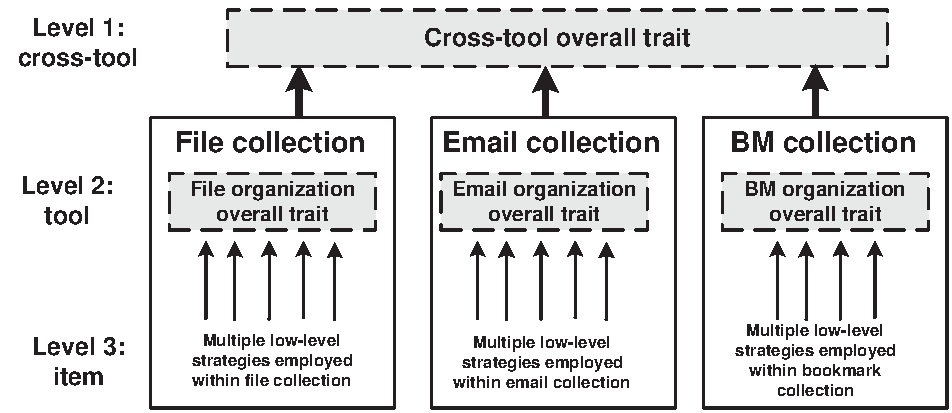
\includegraphics[height=5cm]{pictures/exp-study/PIM-cross-tool-strategies.pdf}
		% fs-fm-comparison.pdf}
	\end{center}
	\caption{Three-level model of an individual's organizing strategies}
	\label{fig:discussion:PIM-cross-tool-strategies}
\end{figure}

% The findings from this study show that you cannot generalize from one level to another. 
This conceptualization emphasises the importance of specifying the level of analysis when talking about phenomena such as organizing strategies.



%%%%%%%%%%%%%%%%%%%%%%%%%%%%%%%%%%%%%%%%%%%%%%%%%%%%%%%%%%%%
% \textit{Include stuff regarding how to talk about strategies}
%%%%%%%%%%%%%%%%%%%%%%%%%%%%%%%%%%%%%%%%%%%%%%%%%%%%%%%%%%%%

%%%%%%%%%%%%%%%%%%%%%%%%%%%%%%%%%%%%%%%%%%%%%%%%%%%%%%%%%%%%%%%%%%%%%%%%%%%%%%%%%%%%%%%%%%%%%%%%%%%%%%%%%%%%%%%%%
%%%%%%%%%%%%%%%%%%%%%%%%%%%%%%%%%%%%%%%%%%%%%%%%%%%%%%%%%%%%%%%%%%%%%%%%%%%%%%%%%%%%%%%%%%%%%%%%%%%%%%%%%%%%%%%%%
%%%%%%%%%%%%%%%%%%%%%%%%%%%%%%%%%%%%%%%%%%%%%%%%%%%%%%%%%%%%%%%%%%%%%%%%%%%%%%%%%%%%%%%%%%%%%%%%%%%%%%%%%%%%%%%%%
%%%%%%%%%%%%%%%%%%%%%%%%%%%%%%%%%%%%%%%%%%%%%%%%%%%%%%%%%%%%%%%%%%%%%%%%%%%%%%%%%%%%%%%%%%%%%%%%%%%%%%%%%%%%%%%%%

%%%%%%%%%%%%%%%%%%%%%%%%%%%%%%%%%%%%%%%%%%
\subsection{Implications for Design}
\label{exp-study:discussion:integration}
%%%%%%%%%%%%%%%%%%%%%%%%%%%%%%%%%%%%%%%%%%

Integration between PIM-tools has been repeatedly put forward as a worthy design aim~\citep{Bellotti:03,Bergman:03,rpb:01a,Dumais:03a,Kaptelinin:03}, but with little empirical support.  It is argued that cross-tool studies such as this one can provide an empirical foundation for such design by highlighting: (1) synergies between tools that can be exploited to improve integration, and (2) differences between tool usage that may indicate barriers to integration.
%%%%%%%%%%%%%%
% PROBLEMS
%%%%%%%%%%%%%%
% In particular, our research is concerned with the problems users encounter across multiple tools whilst performing two PIM-related activities: 1.	Folder organization - the management of items within a folder hierarchy made up of user-defined categories 2.	Reminder Management - the use of items as implicit reminders (or "to-do" items)}
%		Provision of insights into possible upsides and downsides of integration/unification. ID of key issues. See below
\textbf{Section~\ref{exp-study:comparison-problems}} highlighted a number of problems that either, (a) occur in multiple tool contexts, or (b) bridge multiple tools.  The first type of problem can potentially be solved by a cross-tool design strategy, where the same improvement is made to multiple tools.  The second type of problem confirms the potential of improving integration between PIM-tools. Other findings from the study indicate possible routes for integration. % may suggest appropriate routes for cross-tool integration (see \textbf{Section~\ref{exp-study:discussion:integration}}).  % \textbf{Chapter~\ref{chapter:design}} reports the design of a cross-tool integration mechanism. 

%%%%%%%%%%%%%%%%%%%%%%%%%%%%%%%%%%%%%%%
% Link from folder overlap towards WorkspaceMirror}
%%%%%%%%%%%%%%%%%%%%%%%%%%%%%%%%%%%%%%%
% Ideas generated for cross-tool design work later in thesis are summarized.
% \textit{Folder overlap} suggests a mismatch between the production activities (involving multiple PIM tools) and tool-centric PIM support. 
The observation of \textit{folder overlap} in \textbf{Section~\ref{exp-study:Results-folder-overlap}} points to a subset of user activities that involve the management of multiple types of information.  Most overlapping folders corresponded to \textit{roles} and \textit{projects}, suggesting that these concepts may be usefully shared between collections, as in UMEA~\citep{Kaptelinin:03}. However, it should be emphasized that most folders did not overlap. This suggests that: (1) some production tasks are supported by single PIM tools and may not necessarily benefit from increased integration; and (2) users may have different organizational needs in different tools.  Folder overlap forms the empirical basis for the integration technology developed in \textbf{Chapter~\ref{chapter:design}}.

The author notes the potential compatibility for integration of files and \textit{filed} email. Both types of information are either self-created or assessed as having long-term value.  Also, folder overlap was greatest between these collections.  However, complete unification between files and all email (as pointed to by designs such as TaskMaster~\citep{Bellotti:03}) may lead to the disruption of more controlled items (e.g. files, tasks) by unprocessed email. In some cases it may be appropriate not to integrate - but to instead retain separation between tools.  This measured view of the pros and cons of integration is developed further in \textbf{Chapter~\ref{chapter:discussion}}.

The investigation of \textit{organizational dimensions} in \textbf{Section~\ref{exp-study:Results-org-dims}} points to users having different organizational needs in different tool contexts.  It indicates that email contains more \textit{contact}-based folders, whilst bookmark folders are mainly \textit{interest}-based.  This variety suggests users may be constrained by any PIM-tools that are based on specific types of concept. An example in the PIM-integration genre is UMEA~\citep{Kaptelinin:03}, which focuses on \textit{projects}. 

Finally, the discussion in \textbf{Section~\ref{exp-study:discussion:multiple-strategies}} underlines the challenge of PIM design.  Designers must not only cater for individual differences between users, but also for an individual user's \textit{multiple strategies}.  Future design must take account of strategy variation by providing the flexibility to manage different types of information in distinct ways -- both within a single collection, and across collections. For instance, tools should allow users to different items as required, whilst not penalizing those users who do not want to organize. 


% In our future work WE plan to consider integration with other PIM tools (e.g. calendars), and devices involved in PIM (e.g. PDA devices).

%%%%%%%%%%%%%%%%%%%%%%%%%%
% CUE NEED TO EVALUATE
%%%%%%%%%%%%%%%%%%%%%%%%%%


%%%%%%%%%%%%%%%%%%%%%%%%%%%%%%%%%%%%%%%%%%%%%%%%%%%%%%%%%%%%%%%%%%%%%%%%%%%%%%%%%%%%%%%%%%%%%%%%%%%%%%%%%%%%%%%%%
%%%%%%%%%%%%%%%%%%%%%%%%%%%%%%%%%%%%%%%%%%%%%%%%%%%%%%%%%%%%%%%%%%%%%%%%%%%%%%%%%%%%%%%%%%%%%%%%%%%%%%%%%%%%%%%%%
%%%%%%%%%%%%%%%%%%%%%%%%%%%%%%%%%%%%%%%%%%%%%%%%%%%%%%%%%%%%%%%%%%%%%%%%%%%%%%%%%%%%%%%%%%%%%%%%%%%%%%%%%%%%%%%%%
%%%%%%%%%%%%%%%%%%%%%%%%%%%%%%%%%%%%%%%%%%%%%%%%%%%%%%%%%%%%%%%%%%%%%%%%%%%%%%%%%%%%%%%%%%%%%%%%%%%%%%%%%%%%%%%%%

%%%%%%%%%%%%%%%%%%%%%%%%%%%%%%%%%%%%%%%%%%%%%%%%%%%%
%\subsection{Refining the conceptual basis of PIM}
%\label{exp-study:discussion:conceptual-basis}
%%%%%%%%%%%%%%%%%%%%%%%%%%%%%%%%%%%%%%%%%%%%%%%%%%%%
% Other aspects of pim to consider as follows
%%%%%%%%%%%%%%%%%%%%%%%%%%%%%%%%%%%%%%%%%%%%%%%%%%%%
% COMPLEX/DIFFICULT
%%%%%%%%%%%%%%%%%%%%%%%%%%%
%	\item TO PLACE: ANXIETY OF ORDER: even relatively organised users considered themselves messy (i.e. not dictated by number of folders present, as can be failed folders)
%%%%%%%%%%%%%%%%%%%%%%%%%%%%%%%%%%%%%%%%%%%%%%%%%%%%
% Satisficing nature}
%%%%%%%%%%%%%%%%%%%%%%%%%%%
%	\item Organization, maintenance \textit{QUOTE: "`better things to do"'}
%	\item Idiosyncratic cost/benefit trade-off's
%%%%%%%%%%%%%%%%%%%%%%%%%%%%%%%%%%%%%%%%%%%%%%%%%%%%

%The study findings highlight several properties of PIM to be developed in subsequent chapters:
% Insights provided by the study indicate several directions for improving the current conceptual basis for PIM.  
%\begin{itemize}

%%%%%%%%%%%%%%%%%%%%%%%%%%%%%%%%%%%%%%%%%%%%%%%
% CROSS-TOOL NATURE - discussed in more detail below
%		\textbf{Towards a Cross-tool Perspective} -- a different way of looking at the problem.
%		Move from typical tool-centric towards cross-tool view.
%		Inter-relationship between tools is key.
%%%%%%%%%%%%%%%%%%%%%%%%%%%%%%%%%%%%%%%%%%%%%%%
% \subsubsection{PIM as a cross-tool activity}
%%%%%%%%%%%%%%%%%%%%%%%%%%%%%%%%%%%%%%%%%%%%%%%
% \item \textit{PIM as a cross-tool activity} --  Firstly, the study highlighted the cross-tool nature of PIM. Barreau conceptualized the computer as a single abstract PIM system, whereas from a cross-tool perspective it is clear that current PIM-tools constitute a set of parallel yet inter-related systems, in which different types of information are managed in different ways.   This is despite the fact that the different tools are similar in form (e.g. folder-based organizing mechanism).

%%%%%%%%%%%%%%%%%%%%%%%%%%%%%%
% Activities are cross-tool
%%%%%%%%%%%%%%%%%%%%%%%%%%%%%%
% Introduce link to cross-tool abstractions of PIM, e.g. IM and TM. LINK to discussion. \textit{Relate to similar design/theoretical perspectives, e.g. Raskin, Kirsh, Kaptelinin}
% \textbf{Section~\ref{exp-study:comparison-problems}} provided a range of evidence that many PIM-related problems are cross-tool. Aspects of PIM such as information management and task management can be considered as cross-tool: they cut across a wide range of tools.

% OTHER DEVICES
% Note that the study only considered the desktop workspace. One can of course consider PIM across the various computers and mobile devices used by an individual
%	DISCUSS: Relate to beyond the scope of this study (i.e. beyond desktop) as well. Also consider physical comparison, and different physical locations (\textit{QUOTES: bob, sil})


%%%%%%%%%%%%%%%%%%%%%%%%%%%%%%%%%%%%%%%%%%%%%%%%%%%%%
% PIM as a SUPPORTING activity
%%%%%%%%%%%%%%%%%%%%%%%%%%%%%%%%%%%%%%%%%%%%%%%
% \textbf{Section~\ref{exp-study:Results-folder-overlap}} discussed the observation of folder overlap -- folders which existed in multiple PIM-tool contexts. Overlapping folders are interpreted as an indication of production activities that involve the management of multiple types of personal information.
% \item \textit{PIM as a supporting activity} -- \textbf{Chapter~\ref{chapter:discussion}} discusses the view that PIM is a supporting activity.  Some key evidence for this view was uncovered in this study.  Firstly, \textbf{Section~\ref{exp-study:comparison-changes}} observed that the study had a strong ``auditing'' effect on user behaviour, making them think more about PIM than they normally would. %textbf{Section~\ref{exp-study:Results-folder-overlap}} discussed the concept of folder overlap -- folders which existed in multiple PIM-tool contexts.  Overlapping folders are interpreted as an indication of production activities that involve the management of multiple types of personal information.




%%%%%%%%%%%%%%%%%%%%%%%%%%%%%%%%%%%%%%%%%%%%%%%%%%%%%
% PIM as an ONGOING background activity
%%%%%%%%%%%%%%%%%%%%%%%%%%%%%%%%%%%%%%%%%%%%%%%
%\textbf{NEW: pressure/complexity/stress/never-ending}
%\item \textit{PIM as an ongoing activity} -- Although the study was non-longitudinal, some insights into the evolving nature of PIM behaviour were revealed.  In particular, \textbf{Section~\ref{exp-study:comparison-changes}} described participants reports of `historical changes in organizing strategy, including both increases and decreases in filing tendency. These observations partially motivated the longitudinal PIM study reported in \textbf{Chapter~\ref{chapter:main-study}}.

%\end{itemize}

%%%%%%%%%%%%%%%%%%%%%%%%%%%%%%%
% THEORY-BUILDING; CHAPTER 7
%%%%%%%%%%%%%%%%%%%%%%%%%%%%%%%
% WE are continuing our data analysis and are looking to build on current theory in two ways.
% Finally, the study also laid the groundwork for revising the current conceptualization of PIM, in particular regarding its ongoing nature and cross-tool nature.  These are other aspects are considered in more depth in \textbf{Chapter~\ref{chapter:discussion}}. \textit{THINK: need this now, or does it just confuse matters ...IDEA: move all theory-generating stuff to the final discussion}
%%%%%%%%%%%%%%%%%%%%%%%%%%%%%%%%%%%%%%%%%%%
% LINK to later chapter and follow-up work
%%%%%%%%%%%%%%%%%%%%%%%%%%%%%%%%%%%%%%%%%%%
% A portrait of PIM as an ongoing, supporting, cross-tool activity is presented. In the next chapter an extended conceptual framework/model of PIM is presented to incorporate this view.
% This theoretical perspective is developed further in \textbf{Chapter~\ref{chapter:discussion}}.
% The cross-tool nature of PIM is discussed in more depth in the theoretical discussion in \textbf{Chapter~\ref{chapter:discussion}}.
% In \textbf{Chapter~\ref{chapter:discussion}} the conceptual framework outlined in \textbf{Chapter~\ref{chapter:bg}} is extended to reflect the cross-tool, supporting, and ongoing nature of PIM. 

%%%%%%%%%%%%%%%%%%%%%%%%%%%%%%%
% Talking about INFORMATION
% \subsubsection{Descriptive Vocabulary for Personal Information}
% MOVED TO DISCUSSION CHAPTER 15/Apr/04
%%%%%%%%%%%%%%%%%%%%%%%%%%%%%%%

%%%%%%%%%%%%%%%%%%%%%%%%%%%%%%%
% OTHER
%	\item TO PLACE: ANXIETY OF ORDER: even relatively organised users considered themselves messy (i.e. not dictated by number of folders present, as can be failed folders)
%	\item Complex activity -- and many problems.  Highly personal -- can't go to the help desk for support!!  Its your own responsibility
%%%%%%%%%%%%%%%%%%%%%%%%%%%%%


%%%%%%%%%%%%%%%%%%%%%%%%%%%%%%%%%%%%%%%%%%%%%%%%%%%%%%%%%%%%%%%%%%%%%%%%%%
% ALSO: add - what are the methodological implications of the above?
%%%%%%%%%%%%%%%%%%%%%%%%%%%%%%%%%%%%%%%%%%%%%%%%%%%%%%%%%%%%%%%%%%%%%%%%%%
%\textbf{Methodological implications of the above points}
%\begin{itemize}
%	\item Can HCI deal with PIM?
%	\item NB: want to do more than just describe! (MOVE TO METHODOLOGICAL SECTION ABOVE?)
%\end{itemize}

%%%%%%%%%%%%%%%%%%%%%%%%%%%%%%%%%%%%%%%%%%%%%%%%%%%%%%%%%%%%%%%%%%%%%%%%%%%%%%%%%%%%%%%%%%%%%%%%%%%%%%%%%%%%%%%%%
%%%%%%%%%%%%%%%%%%%%%%%%%%%%%%%%%%%%%%%%%%%%%%%%%%%%%%%%%%%%%%%%%%%%%%%%%%%%%%%%%%%%%%%%%%%%%%%%%%%%%%%%%%%%%%%%%
%%%%%%%%%%%%%%%%%%%%%%%%%%%%%%%%%%%%%%%%%%%%%%%%%%%%%%%%%%%%%%%%%%%%%%%%%%%%%%%%%%%%%%%%%%%%%%%%%%%%%%%%%%%%%%%%%
%%%%%%%%%%%%%%%%%%%%%%%%%%%%%%%%%%%%%%%%%%%%%%%%%%%%%%%%%%%%%%%%%%%%%%%%%%%%%%%%%%%%%%%%%%%%%%%%%%%%%%%%%%%%%%%%%



%%%%%%%%%%%%%%%%%%%%%%%%%%%%
\subsection{Conclusion}
\label{exp-study:discussion:conclusion}
%%%%%%%%%%%%%%%%%%%%%%%%%%%%
% * Relate carefully to aims of chapter
% * Discuss relative to overall thesis
%%%%%%%%%%%%%%%%%%%%%%%%%%%%
% Overall: success of study, what it contributed to the thesis} 
% Helped me understand domain. The study identified/highlighted, provided background into the area. Insights into PIM. ID of key issues. Rich picture - raised many interesting points
% Evidence for user problems and dissatisfaction with current tool sets, struggle, confirmed that worthwhile area for research!
% Consider as requirements gathering section. Interesting design ideas and suggestions from users 

It is argued that the study reported in this chapter was successful in meeting its objectives.  A wide range of findings have been presented. In addition to helping the author gain a foundational understanding of the research domain, a number of novel contributions were also made.  Key contributions include improved understanding of the nature of organizing strategies within and across PIM-tools, and the design implications presented above.  % However, it is re-emphasised that the exploratory nature of the techniques used, the complex nature of the phenomena investigated, and the relatively small number of participants involved, mean that the results should be considered indicative only.
% he main contribution from the study was the investigation into the cross-tool nature of PIM.  Secondary contributions include the nature of PIM within the tool-specific contexts of files, email and bookmarks.
% The results should be treated as exploratory and indicative due to the small sample size involved.

%%%%%%%%%%%%%%%%%%%%%%%%%%%%%%%%%%%%%%%%%%
% Provide linkage to remaining chapters
%%%%%%%%%%%%%%%%%%%%%%%%%%%%%%%%%%%%%%%%%%
This study provides an empirical foundation for later chapters. Firstly, it provides empirical motivation for the design work in \textbf{Chapter~\ref{chapter:design}}.  In particular, the observation of folder overlap lead to the invention of the folder-mirroring principle. % , instantiated as the WorkspaceMirror prototype.
% Findings acted as requirements (core empirical grounding)for main design-based research process.
The observation of changes in organizing strategy, motivated the need for the longitudinal study reported in \textbf{Chapter~\ref{chapter:main-study}}. % Finally, \textbf{Section~\ref{exp-study:discussion:conceptual-basis}} laid the groundwork for the theoretical discussion of PIM offered in \textbf{Chapter~\ref{chapter:discussion}}.
% lead to the development of the cross-tool perspective employed in the thesis.









% \textit{This draft of Chapter 4 EXPLORATORY STUDY was printed \today}
%%%%%%%%%%%%%%%%%%%%%%%%%%%%%%%%%%%%%%%%%%%
%% END CONCLUSION/CHAPTER 4 EXP STUDY
%%%%%%%%%%%%%%%%%%%%%%%%%%%%%%%%%%%%%%%%%%%

%%%%%%%%%%%%%%%%%%%%%%%%%%

% CHECK ALL SECTIONS!

%%%%%%%%%%%%%%%%%%%%%%%%%%


% %%%%%%%%%%%%%%%%%%%%%%%%%%%%%%

% chapter 5 - Cross-tool Design

% %%%%%%%%%%%%%%%%%%%%%%%%%%%%%%

\chapter{Cross-tool Design}

\label{chapter:design}

%%%%%%%%%%%%%%%%%%%%%%%%%%%%%%%%%%%%%%%%%%%%%%%%%%%%%%%%%%%%%%%%%%%%%%%%%%%%%%%%%%%%%%%%%
% CHAPTER 5 - DESIGN
%%%%%%%%%%%%%%%%%%%%%%%%%%%%%%%%%%%%%%%%%%%%%%%%%%%%%%%%%%%%%%%%%%%%%%%%%%%%%%%%%%%%%%%%%
% Richard Boardman PhD Thesis
% Improving Tool Support for Personal Information Management
%%%%%%%%%%%%%%%%%%%%%%%%%%%%%%%%%%%%%%%%%%%%%%%%%%%%%%%%%%%%%%%%%%%%%%%%%%%%%%%%%%%%%%%%%
% Method notes
%%%%%%%%%%%%%%%%%%
%	How strictly to follow Carroll's methodology in terms of strict design rationale
% and claims analysis? Root in strong psyhological findings?
%		Or do I have a weasel? Claims inherent in bog-standard hierarchy?}
% Form of needs/requirements - relate this to evaluation criteria?
%%%%%%%%%%%%%%%%%%%%%%%%%%%%%%%%%%%%%%%%%%%%%%%%%%%%%%%%%%%%%%%%%%%%%%%%%%%%%%%%%%%%%%%%%
% DESIGN THEORY: need to take care!
% 	TOPLACE: \section{Design as Research} \label{design:design-as-research}
% 	Consider placement of role of design in HCI research here}
%	Relate to nature of design -- purposeful/creative, ITERATIVE, unbounded/never-ending}
%%%%%%%%%%%%%%%%%%%%%%%%%%%%%%%%%%%%%%%%%%%%%%%%%%%%%%%%%%%%%%%%%%%%%%%%%%%%%%%%%%%%%%%%%
%	REMEMBER ANGELA'S CLIFF!
%%%%%%%%%%%%%%%%%%%%%%%%%%%%%%%%%%%%%%%%%%%%%%%%%%%%%%%%%%%%%%%%%%%%%%%%%%%%%%%%%%%%%%%%%
% Need for definitions: PIM tool/software/application
% vs. cross-tool/means of integration/integrating mechanism 
%%%%%%%%%%%%%%%%%%%%%%%%%%%%%%%%%%%%%%%%%%%%%%%%%%%%%%%%%%%%%%%%%%%%%%%%%%%%%%%%%%%%%%%%%
% WORDS
% design rationale/justification/defense
% leverage, motivate, exploit
% strawman/test-bed/research-vehicle
%%%%%%%%%%%%%%%%%%%%%%%%%%%%%%%%%%%%%%%%%%%%%%%%%%%%%%%%%%%%%%%%%%%%%%%%%%%%%%%%%%%%%%%%%
% Key aspects of chapter:
% Following design-science paradigm
% Exploration in cross-tool design space
% Decision to focus on one design
% Communicate how the design came into being
%%%%%%%%%%%%%%%%%%%%%%%%%%%%%%%%%%%%%%%%%%%%%%%%%%%%%%%%%%%%%%%%%%%%%%%%%%%%%%%%%%%%%%%%%
%	Ways of improving support for PIM:
% 	(1) improve support
%		(2) change user practice
% 	(3) dovetailing of the two}
%%%%%%%%%%%%%%%%%%%%%%%%%%%%%%%%%%%%%%%%%%%%%%%%%%%%%%%%%%%%%%%%%%%%%%%%%%%%%%%%%%%%%%%%%


%%%%%%%%%%%%%%%%%%%%%%%%%%%%%%%%%%
\section{Introduction}
\label{design:introduction}
%%%%%%%%%%%%%%%%%%%%%%%%%%%%%%%%%%

%%%%%%%%%%%%%%%%%%%%%%%%%%%%%%%%%%%%%%%%%%%
% General intro
%		Relate to overall PhD aims
% Perspective to mention: Continued operationalization of cross-tool
% research methodology outlined in \textbf{Chapter~\ref{chapter:research_agenda}}, 
%%%%%%%%%%%%%%%%%%%%%%%%%%%%%%%%%%%%%%%%%%%
This chapter reports the design, implementation, and initial evaluation of the \textit{WorkspaceMirror} prototype, abbreviated to WM henceforth.  WM provides a novel integration mechanism between three collections of personal information (files, email and bookmarks) based on the principle of \textit{folder mirroring} -- the sharing of organizational structure across PIM-tools.


%%%%%%%%%%%%%%
% DESIGN AIMS
%%%%%%%%%%%%%%
%%%%%%%%%%%%%%%%%%%%%%%
% METHOD/CROSS-TOOL
%%%%%%%%%%%%%%%%%%%%%%%
% Explore how to design along cross-tool dimension. Driving concern: operationalize  cross-tool principles in terms of design recommendations -- making cross-tool perspective ``operationalizable''
% \item \textit{Focus on one novel \textit{cross-tool} support for PIM -- i.e. creation of an artefact that embodies implicit psychological claims.}
%%%%%%%%%%%%%%%%%%%%%%%%%
% Method: Form of design objectives
%%%%%%%%%%%%%%%%%%%%%%%%%%%%%%%%%%%%%%%%%
%%%%%%%%%%%%%%%%%%%%%%%%%%%%%%%%%%
% Design philosophy/perspective
% * must use these to drive aims or vice versa
% motivating factors
% specify Design Theory and Approaches influencing my work?
%%%%%%%%%%%%%%%%%%%%%%%%%%%%%%%%%%
% Design perspective (driven by critique of previous design/technology and my own cross-tool perspective:):
%%%%%%%%%%%%%%%%%%%%%%%%
% Previous work:
% %%%%%%%%%%%%%%%
% lack of empirical motivation
% complex. Aimed at techies?
% revolutionary.  Therefore hard to learn, implement, evaluate.
% Lack of evaluation.  Therefore bottom line: little contribution to knowledge
%%%%%%%%%%%%%%%%%%%%%%%%%%%%%%%%%%%%%%
% ADD: Discuss in terms of T/A cycle
%%%%%%%%%%%%%%%%%%%%%%%%%%%%%%%%%%%%%%
% Desire to complete the cycle THINK: MOVE EARLIER Base on Carroll and Rosson's Task-Artefact Theory - artefact as theory. Task provides requirements for artefact, AND artefact redefines/provides new possibilities for the task.
%%%%%%%%%%%%%%%%%%%%%%%%%%%%%%%%%%%%%%%%%%%%%%%%%%%%%%%%%%%%%%%%%%%%%%%%%%%%%%%%
% ADD: Cross-tool perspective
% Each objective entails building on the limitations of previous design work in this area
% As well as these overall objectives, a key consideration was to improve upon the limitations of previous PIM prototypes as highlighted in the literature review (\textbf{Chapter~\ref{chapter:review}}).
% These are discussed as follows. % UPDATE SECTION NUMBER
%%%%%%%%%%%%%%%%%%%%%%%%%%%%%%%%%%%%%%%%%%%%%%%%%%%%%%%%%%%%%%%%%%%%%%%%%%%%%%%%
%Rooted in cross-tool perspective (i.e. principled)
%\begin{itemize}
%		\item Perspective as design principled approach
%		\item Focus here: improve integration/consistency/unification between PIM tools that make up the personal digital workspace. Focus: storage/organization.
%		\item Cross-tool solutions to cross-tool problems
%		\item \textit{THINK: integration between tools or between activities}
%%%%%%%%%%%%%%%%%%%%%%%%%%%%%%%%%%%%%%%%%%%%%%%%%%%%%%%%%%%%%%%%%%%%%%%%%%%%%%%%
\subsection{Aims}
\label{design:aims}
%%%%%%%%%%%%%%%%%%%%%%%%%%%%%%%%%%%%%%%%%
% This section presents the objectives of the design work, and the design approach that was taken.
The design component of this thesis had three high-level objectives, each relating to a limitation of previous design work in this area:
\begin{enumerate}

%%%%%%%%%%%%%%%%%%%%%%%%%%%%%%%%%%%%%%%%%
% DESIGN TOOL WITH Empirical grounding
%%%%%%%%%%%%%%%%%%%%%%%%%%%%%%%%%%%%%%%%%
% Basis in problems observed in exploratory study. Grounded in empirical evidence. lack of empirical motivation
% The design rationale must be grounded in empirical data
% A second key criticism that can be levelled at many previous prototypes is that they have not been grounded in empirical data, but rather founded on  (see ).  \citet{Carroll:00} discusses the importance of empirical grounding.  
% The design should be grounded in findings from the exploratory study.
%  --  (i.e. answer the design question: how can integration between existing PIM tools be enhanced to better support user needs?) 
\item \textit{To propose a design that offers a new form PIM integration to better meet user needs} -- \textbf{Chapter~\ref{chapter:review}} criticises a number of previous research prototypes in this area for a lack of empirical grounding.  Instead, many have been founded on designer intuition.  To avoid similar criticism, the author set out to ground his design efforts in findings from \textbf{Chapter~\ref{chapter:exploratory_study}}.

\item \textit{To implement the design with an aim of performing a long-term evaluation} -- This was to counter a second limitation of previous prototypes: that in most cases they have not been evaluated to test designers' claims.  Therefore, any implementation had to be sufficiently robust to sustain long-term usage in real-world conditions.  
%  to:  (1) explore issues related to improving integration between PIM tools; and (2) develop appropriate methodology for evaluating PIM tools.

\end{enumerate}

%%%%%%%%%%%%%%%%%%%%%%%%%%%%%%%
\subsection{Design Approach}
%%%%%%%%%%%%%%%%%%%%%%%%%%%%%%%
%%%%%%%%%%%%%%%%%%%%%%%%%%
% incremental approach
%%%%%%%%%%%%%%%%%%%%%%%%%%
% Move away from radical invention towards evolutionary, incremental design, measured step.
% This stance is contrasted with that taken by more ambitious ``PIM-unifying'' systems that have been proposed in the past.
% Best chance to complete the cycle
% Don't cross the streams!
% summarized in \textbf{Chapter~\ref{chapter:review}} has produced inventive \textit{revolutionary} designs which offer an alternative to current tools. Although innovative, such designs may offer a barrier to successful uptake and evaluation.
%%%%%%%%%%%%%%%%%%%%%%%%%
% Extra Carroll depth
%%%%%%%%%%%%%%%%%%%%%%%%%
% Have to correctly relate incremental, hill-climbing and cumulative
% Carroll proposes three modes of design reasoning that enable cumulative design, along with their positive and negative aspects: (1) \textit{hill-climbing}, (2) \textit{principled emulation}, and (3) \textit{activity modelling}.
% The second paradigm, principled emulation involves applying designs from other domains. The third paradigm, activity modelling is based on the study of user practices. % TODO: expand on this
% Furthermore, revolutionary design is hard to build on, and \textbf{Chapter~\ref{chapter:review}} observes how the products of such design tend to complex and hard to evaluate.
In contrast to most previous work in this area, the design reported here was deliberately \textit{incremental} -- aimed at extending, rather than replacing existing technology.  This relates to a third criticism of previous work made in \textbf{Chapter~\ref{chapter:review}}: that there has been an over-focus on \textit{revolutionary design}, the innovation of radical alternatives to current tools.  Although many interesting designs have been proposed, such \textit{radical invention} does not necessarily entail a strong contribution in terms of HCI knowledge, especially if no evaluation has been performed.  
In response, a number of researchers have emphasized the need for an iterative, incremental process of design~\citep{ml:88,newman:95,Whittaker-rta:00,Carroll:00}.  This approach has been termed cumulative design, or ``hill climbing''~\citep{Carroll:00}.  In the context of this thesis, an incremental approach was chosen for the following reasons:
\begin{enumerate}

%%%%%%%%%%%%%%%%%%%%%%%%%%%
% Import of evaluation.
%%%%%%%%%%%%%%%%%%%%%%%%%%%
% Facilitate thorough evaluation
% Thus although a range of exciting techniques have been proposed it is difficult 
% third benefit of incremental design is that it facilitates systematic evaluation~.  By making limited changes to the existing personal information environment, it was envisaged that it would be easier to associate specific changes with the design intervention. 
\item \textit{To enable effective evaluation} -- As noted above, a key aim of the work reported in this chapter was to enable effective evaluation.  One downside of radical invention is that it is difficult to measure specific improvements as so many interface aspects may change~\citep{Carroll:00}.  \citet{newman:95} argue that incremental, localized changes that are well-understood and result in subtle improvements, are to be preferred over more ambitious changes which may result in complex side effects.  

%%%%%%%%%%%%%%%%%%%%%%%%%%%%%%%%%%%%%%%%%%%%
% Familiar concepts - promote learnability
%%%%%%%%%%%%%%%%%%%%%%%%%%%%%%%%%%%%%%%%%%%%
%  it was hoped that ease of use would be promoted.
% To promote learnability/user familiarity. 
% incremental changes to retain familiarity - not asking users to start from fresh)
\item \textit{To promote user familiarity} --  By basing design on existing technology, it was envisaged that the likelihood of system uptake would be increased.  Employing familiar concepts and tools will mean that users have less to learn~\citep{Carroll:00}.

%%%%%%%%%%%%%%%%%%%%%%%%%%%%%%%%%%%%%%%%%%%%%%%%%%%%%%%%%%%%%%%%%
% easier bootstrapping - Supports aim for long-term evaluation. 
%%%%%%%%%%%%%%%%%%%%%%%%%%%%%%%%%%%%%%%%%%%%%%%%%%%%%%%%%%%%%%%%%
% prime aim was to ensure compatibility with the existing personal information environment.  
% bootstrapping and minimize disruption to the user
\item \textit{To promote system up-take} -- Building on current tools implicitly encourages compatibility with previous data formats.  It was envisaged that this would make long-term evaluation more straightforward, since a tool that can be easily integrated into a user's existing tool-set is more likely to be used.  % In addition, at the end of the evaluation, it was intended that the prototype could be easily removed with minimal impact.
A major concern was to avoid prospective users having to go through complex data-import processes, or abandon carefully nurtured collections of personal information in favour of an unproven technology.  

%%%%%%%%%%%%%%%%
% Achievable
%%%%%%%%%%%%%%%
% influence of external constraints/pragmatics on choice of method}
\item \textit{To encourage an achievable design goal} -- Another key concern was that the design and implementation needed to be achievable in the context of the limited time and man-power resources available. An incremental approach allowed the author to build on previous design expertise manifested in already available tools.

\end{enumerate}

%%%%%%%%%%%%
% DOWNSIDE
%%%%%%%%%%%%
% also argues in favour of incremental design (also known as cumulative design or ``hill climbing''). He discusses how this approach offers familiarity for users, and the benefits of grounding in previous design expertise.  However, he also observes potential downsides including the possibility of inheriting from poor previous designs, and the limitations to local optimization. 
\citet{Carroll:00} observes a fundamental limitation of incremental design.  Along with the benefits of building on previous design expertise comes the risk of inheriting previous design limitations.  Therefore, the designer may be constrained to making little more than local optimizations.
%%%%%%%%%%%%%%%%%%%%%%%%%%%%%%
% Can change later anyway
%%%%%%%%%%%%%%%%%%%%%%%%%%%%%%
% Additional functionality can be added based on initial evaluation results.
However, it is observed that an incremental design approach facilitates subsequent iterative refinement once initial changes have been evaluated.  In other words, following an incremental strategy does not mean that further more ambitious changes cannot be made. 

%%%%%%%%
% UCD
%%%%%%%%
%%%%%%%%%%%%%%%%%%%%%%%%%%%%%%%%%%%%%%%%%%%%%%%%%%%%%%%%%%%%%%%%%%%%%%%%%%%%
\subsection{Structure of the Chapter}
%%%%%%%%%%%%%%%%%%%%%%%%%%%%%%%%%%%%%%%%%%%%%%%%%%%%%%%%%%%%%%%%%%%%%%%%%%%%
% Adopt \textbf{standard usability engineering-style loop} (Dix, Preece, Whiteside, Nielsen) -- \textit{iterative prototyping and evaluation of usability is key}, (cf. User-centred Design (Norman and Draper), Scenario-based Design~\citep{Carroll:00}, yeartest~\citen{Carroll:00}.
%%%%%%%%%%%%%%%%%%%%%%%%%%%%%%%%%%%%%%%%%%%%%%%%%%%%%%%%%%%%%%%%%%%%%%%%%%%%
% Method: Description of design method (can I claim participatory design?)
% This is a mismatch of method, design rationale, and desired characteristics of target design
%%%%%%%%%%%%%%%%%%%%%%%%%%%%%%%%%%%%%%%%%%%%%%%%%%%%%%%%%%%%%%%%%%%%%%%%%%%%
% The design methodology followed by the candidate is summarized:
% Design work was carried out as follows.
%%%%%%%%%%%%%%%%%%%%%%%%%%
% Analysis of problems -> initial design space
%%%%%%%%%%%%%%%%%%%%%%%%%%
% Analysis of key problems highlighted in exploratory study (workspace-wide problems)
% Staking out Cross-tool Requirements.
% Initially outline potential design space opened up by findings from the exploratory study. Not Small tool-centric problem in many places/Larger problem that bridges tool. 
% BRAINSTORMING
This chapter reports how an incremental perspective was employed within a user-centred design process.
The first step of the design work was to brainstorm improvements to address user problems identified in the exploratory study reported in \textbf{Chapter~\ref{chapter:exploratory_study}}.  Since a key aim was to investigate routes for improving integration between PIM-tools,  a focus was taken on the problems in \textbf{Section~\ref{exp-study:comparison-problems}} that bridged multiple PIM-tool contexts. 
% INITIAL DESIGN SPACE
% , and associated empirical and theoretical design rationale.
% A range of paper and working prototypes were developed, and assessed by the author.
% Several users asked for feedback
% \textbf{Section~\ref{design:initial-forays}} describes this initial cross-tool design space of problems, and potential solutions.
\textbf{Section~\ref{design:initial-forays}} presents two design avenues which emerged from the exploratory study findings.
% DESIGN FOCUS
% Focus on design ideas that offer increased integration between PIM tools
% One particular idea/design idea to be focused on.
% Consider design trade-off's and consequences
% Making design rationale explicit. \textbf{Design Rationale} techniques to record decisions made in design process and context of those decisions (design space, process-oriented, psychological claims)
Due to time constraints, the thesis focused on one of the candidate design routes, that of \textit{folder-mirroring}. The rationale behind this design focus is presented in \textbf{Section~\ref{design:sharing-mirroring}}, along with a description of the design. %, along with a description of how the design evolved over time. The design rationale behind key decisions is also described, along with open issues that remained before implementation.
% IMPLEMENTATION
\textbf{Section~\ref{design:wm-prototyping}} reports the development of a folder-mirroring prototype, called \textit{WorkspaceMirror} (WM).
% initial evaluation
\textbf{Section~\ref{design:feasibility-study}} then presents an initial evaluation that was carried out to assess the viability of the folder-mirroring principle.  
% COMPARISON compares the principle of folder-mirroring with other approaches to PIM-integration.
Finally, \textbf{Section~\ref{design:discussion}} contrasts WM with other research prototypes.
% \textbf{Section~\ref{design:design-extensions}} details possible design extensions to the core functionality. 

%%%%%%%%%%%%%%%%%%
\subsection{Contributions}
%%%%%%%%%%%%%%%%%%
% Focus on novel cross-tool design of WorkspaceMirror as a major deliverable. As a straw-man to investigate potential to unify PIM support. Incremental design.
% This chapter's main contribution is the design and implementation of WM.
% As well as being an instance of one possible form of PIM-integration, WM is proposed as a research vehicle to enable the investigation of issues relating to PIM-integration.
This chapter makes two main contributions to the thesis:
\begin{enumerate}
\item \textit{The design and implementation of the WM prototype} --  As well as being a novel PIM-integration mechanism, WM acted as a research vehicle to enable the investigation of general issues relating to PIM-integration.
\item \textit{The results from the initial formative evaluation of WM} -- These results confirmed the worth of pursuing a more in-depth evaluation. \textbf{Chapter~\ref{chapter:main-study}} reports a follow-up longitudinal evaluation of a modified version of WM which incorporated suggestions from the initial evaluation.
\end{enumerate}

%%%%%%%%%%%%%%%%%%%%%%%%%%%%%%%%%%%%%%%%%%%%%
% relate to other chapters: past and future
%%%%%%%%%%%%%%%%%%%%%%%%%%%%%%%%%%%%%%%%%%%%%
% The design was motivated by conclusions from the literature review in \textbf{Chapter~\ref{chapter:review}}, along with findings from the exploratory study in \textbf{Chapter~\ref{chapter:exploratory_study}}. % The next chapter, \textbf{Chapter~\ref{chapter:main-study}} describes the longitudinal formative evaluation of WM.


%%%%%%%%%%%%%%%%%%%%%%%%%%%%%%%%%%%%%%%%%%%
% \subsection{Structure of the Chapter}
%%%%%%%%%%%%%%%%%%%%%%%%%%%%%%%%%%%%%%%%%%%
%%%%%%%%%%%%%%%%
% Structure
%%%%%%%%%%%%%%%%
% The chapter is structured as follows.
% Firstly, \textbf{Section~\ref{design:aims}} discusses design aims and approach. 
% \textbf{Section~\ref{design:sharing-mirroring}} discusses the focus that was taken on one of these: \textit{folder-mirroring}. \textbf{Section~\ref{design:comparison}} compares folder-mirroring with related prototypes to date.
%  \textit{folder-sharing}, and details a particular approach to folder-sharing, . % specialization?
% Next, \textbf{Section~\ref{design:wm-prototyping}} describes the implementation of WM based on the folder-mirroring principle. \textbf{Section~\ref{design:feasibility-study}} reports an initial field trial of WM to assess its viability.  Finally, \textbf{Section~\ref{design:summary}} summarises the work presented in the chapter and discusses the contributions made.  This section also proposes the theoretical concept of a cross-tool artefact, and discusses consequent methodological considerations for the evaluation of such an artefact.
%  that lead from the cross-tool design work presented in this chapter.
% which were taken into account during the evaluation work reported in \textbf{Chapter~\ref{chapter:main_study}}.

%%%%%%%%%%%%%%%%%%%%%%%%%%%%%%%%%%%%%%%%%%%%%%%%%%%%%%%%%%%%%%%%%%%%%%%%%%%%%%%%%%
%%%%%%%%%%%%%%%%%%%%%%%%%%%%%%%%%%%%%%%%%%%%%%%%%%%%%%%%%%%%%%%%%%%%%%%%%%%%%%%%%%
%%%%%%%%%%%%%%%%%%%%%%%%%%%%%%%%%%%%%%%%%%%%%%%%%%%%%%%%%%%%%%%%%%%%%%%%%%%%%%%%%%
%%%%%%%%%%%%%%%%%%%%%%%%%%%%%%%%%%%%%%%%%%%%%%%%%%%%%%%%%%%%%%%%%%%%%%%%%%%%%%%%%%

%%%%%%%%%%%%%%%%%%%%%%%%%%%%%%%%%%%%%%%%%%%%%%%%
%%%%%%%%%%%%%%%%%%%%%%%%%%%%%%%%%%%%%%%%%%%%%%%%
\newpage
\section{Initial Forays in a Cross-tool Design Space}
% \section{Staking out the cross-tool design space}
\label{design:initial-forays}
%%%%%%%%%%%%%%%%%%%%%%%%%%%%%%%%%%%%%%%%%%%%%%%%
% THINK: Present design rationale in the form of claims? (upsides/downsides)}
% Can I avoid "creative leap" syndrome?
% Method: Form of design rationale in describing design
% Cover all envisaged designs, or just WorkspaceMirror?
% Wording: Potential designs. candidate designs
%%%%%%%%%%%%%%%%%%%%%%%%%%%%%%%%%%%%%%%%%%%%%%%%

%%%%%%%%%%%%%%%%%%%%%%%%%%%%%%%%%%
% 2 types of cross-tool problem
% 1. within-tool -- intra tool, consistent
% 2. cross-tool -- need for coordination
%%%%%%%%%%%%%%%%%%%%%%%%%%%%%%%%%%
% Informed by data from the exploratory study, an initial design space was developed by the author. Potential routes for design work are identified, motivated by specific findings from the exploratory study, and discussed in terms of the conceptual framework outlined in Chapter 5. The considered design routes are discussed (see \textbf{Figure~\ref{fig:design:initial_designs}}):
% Initial prototyping carried out to explore the viability of each design is described.
%Discuss the following for each:
%\begin{itemize}	
%		\item Motivating results from exploratory study.
%			\item their design rationale, synthesis of ideas and theories influencing design. 
%			\item support for design decisions made (TA, LR, CTF, ES)
%			\item inherent trade-off's, balance arguments for and against
%			\item What aspects of PIM are they supporting?
%			\item How they fit into cross-tool analytical framework
%			\item Comment on generality across users, severity of problem they're solving
%			\item i.e. generally add more detail with DIAGRAMS for each
%\end{itemize}
% ADD: provide scenarios for each?
% ADD compare to related research?

%%%%%%%%%%%%%%%%%%%%%%%%%%%%%%%%%%%%%%%%%%%%%%%
% The following designs emerged from the data
%%%%%%%%%%%%%%%%%%%%%%%%%%%%%%%%%%%%%%%%%%%%%%%
% \textit{Two types of cross-tool problem were identified in \textbf{Chapter~\ref{chapter:exploratory_study}}: (1) within-tool problems that occur in multiple tool contexts (e.g. ADD EXAMPLE), and (2) cross-tool problems that bridge multiple tools (e.g. ADD EXAMPLE).}
% This section surveys the initial design space that emerged from the exploratory study findings.  The findings reported in \textbf{Chapter~\ref{chapter:exploratory_study}} included several sets of user needs which corresponded with potential routes for improved design integration.  In this section, two sets of cross-tool problems are described, along with the initial design prototyping carried out by the author. Each problem involves multiple PIM-tools.
This section reports initial incremental design and prototyping directed at solving two of the \textit{cross-tool} problems identified in \textbf{Section~\ref{exp-study:comparison-problems}}.  Note that both are incremental adjustments to commonly available PIM-tools.

% The first concerns the use of different types of information as reminders.  The second relates to the need to organize different types of information in separate folder structures.

%%%%%%%%%%%%
% Naming
%%%%%%%%%%%%
% provide an enhanced naming mechanism, consistent across all PIM tools. Motivation by user problems relating to naming items.
% QUESTION: are there any quotes I can add? \textbf{QUOTES}
%%%%%%%%%%%%%%%%%%%%%%%%%%%
% \subsection{Naming items}
%%%%%%%%%%%%%%%%%%%%%%%%%%%
% Several participants complained of difficulties naming items of information in various tools.  In particular, the naming of bookmarks was seen as unsatisfactory by several participants.  They complained that the default name assigned to new bookmarks (that of the title meta-data from the page they pointed to) were often inappropriate.  Furthermore, changing the name from the default setting was seen as clumsy. For instance, using some content from within the page to name the newly created bookmark involved a laborious process of selecting the bookmark, and then copying and pasting the text.  One participant complained that it was not easily possible to rename email subjects.  The naming problem space can be considered cross-tool in the sense that participants encountered difficulties within multiple PIM-tools. Participants complained of the lack of consistency between PIM-tools regarding functionality such as naming items. 
% A new mechanism was developed by the author to make it easier to name bookmarks with arbitrary content from the referenced web page, termed \textit{in-line naming}.  Instead of creating the bookmark and then renaming it, the user can first select some text on a web-page, and then via a context-menu, specify that text as the name of a new bookmark referencing that page.  A working prototype was developed by the author in the context of MS-Internet Explorer.  Furthermore, the lack of consistency between tools in terms of naming functionality could be addressed by offering in-line naming and renaming of items across all PIM-tools.
% based on the \textit{Consistent Naming Principle}: users should have a consistent mechanism for naming an item in all PIM-tools, be it a file, email or bookmark.  The envisaged design allowed the user to select any arbitrary text in an item, and via .  


%%%%%%%%%%%%%%%%%%%%%%%%%%%%%%%%%%
% Todo highlighting + groupable
%%%%%%%%%%%%%%%%%%%%%%%%%%%%%%%%%%%%%%%%%%%%%%%%%%%%%
\subsection{Highlighting and Gathering To-do Items}
%%%%%%%%%%%%%%%%%%%%%%%%%%%%%%%%%%%%%%%%%%%%%%%%%%%%%

Several participants in the exploratory study mentioned problems relating to the use of information as reminders.  These included a lack of consistency between different tools regarding support offered for highlighting an item as a \textit{to-do item}. A second problem was that it was hard to gather together to-do items from different tools.
% For instance, MS-Outlook allows the ``flagging'' of messages within the email view. However, the Windows file manager and MS-Internet Explorer do not offer any similar functionality.  A second problem reported by a number of participants was that it was hard to gather together related items, such as to-do items. % Note that no participants made use of dedicated to-do managers, such as the ``Tasks view'' in MS-Outlook 

% MOVE TO CHAPTER 4?
The author's proposed solution allowed any item of information to be highlighted and marked as a to-do.  To-do items are highlighted in a consistent manner across all tools via a standardized context-menu mechanism.  At the same time, a reference to each new to-do item is added to a unified list.  An initial proof-of-concept was developed on MS-Windows using MS-Visual Basic 6.0, allowing any desktop icon, file, or bookmark, to be selected and highlighted as a to-do.  This resulted in the icon background changing to red. A short-cut to the item was also added to the MS-Outlook ``tasks view''.  However, it was not possible to provide the same mechanism for highlighting emails due to imitations on the MS-Outlook object model.  This design can be related to the functionality present in attribute-based systems that allow users to label arbitrary pieces of personal information with an attribute such as ``to-do'' or ``important'', e.g.\citep{dourish:99a}.  The author's work can be differentiated due to the incremental design stance of providing functionality on top of standard PIM-tools.
% Several participants observed the lack of consistency between PIM-tools regarding support offered for highlighting an item as a \textit{to-do}.  For instance, MS-Outlook allows the ``flagging'' of messages within the email view, or the management of a separate list of to-do items in the ``Tasks view''.  Emails or files can be dragged into the separate to-do list. However, the to-do item is not highlighted in its original context and is treated as a separate entity, \textit{P22: ``You sit and look at your inbox - and you have to type or write the to-do item separately, and you can't very easily make an email a to-do item. It involves something that I regard ... a redundant transformation. You know basically converting one form of data into another which doesn't add anything. You know there's no added value there - you don't have any easy way of pushing data from one tool to another, copying it from one space to another''}. % and are embedded within new to-do items.



%%%%%%%%%%%%%%%%%%%%%%%%%%%%%%%%
% Add initial user feedback?
%%%%%%%%%%%%%%%%%%%%%%%%%%%%%%%%

%%%%%%%%%%%%%%%%%%%%
% ADD MORE DETAIL HERE?
% REASONS FOR FOCUS
% \textit{The rationale for focusing on the folder-mirroring is discussed.  }
%%%%%%%%%%%%%%%%%%%%%%%%%%%%%%%%%%%
\subsection{Managing Multiple Types of Information in Parallel}
%%%%%%%%%%%%%%%%%%%%%%%%%%%%%%%%%%%

A second area of difficulty reported by users related to the need to manage distinct collections of personal information across a range of PIM-tools, each with a distinct organizational structure.
%%%%%%%%%%%%%%%%%%%%%%%%%%%%%%
% Various options available
%%%%%%%%%%%%%%%%%%%%%%%%%%%%%%
% The design-space relating to different ways of sharing folder structure is outlined. 
After initial brainstorming, two possible approaches were identified to make it easier for users organize information in multiple PIM-tools:
\begin{enumerate}

%%%%%%%%%%%%%%%%%%%%%%%%%%%%%%%%%%%%%
% More ambitious: folder sharing
%%%%%%%%%%%%%%%%%%%%%%%%%%%%%%%%%%%%%
% cite Presto?
% think generalize `folder' to `container'
% The more ambitious approach to folder-sharing involves \textit{unified storage}. 
\item \textit{Folder sharing} -- This would allow the storage of multiple types of information (e.g. files and email) within a consolidated folder structure.  Two key problems were identified with this route. First, it was not clear how such a scheme would co-exist with current tools, and whether users would employ it in preference to those tools.  Secondly, an initial investigation of the technical feasibility of folder-sharing on MS-Windows, concluded that it was beyond the time and manpower resources of a single PhD researcher.
% In other words the same physical storage would be accessed via multiple PIM-tools.  Two key problems were identified with this route: (1) barriers to usage, and (2) ease of implementation.  First, it was not clear how such a scheme would co-exist with current tools. A prime aim was to carry out the long-term evaluation of a designed artefact.  For this to happen it was seen to be essential that the tool integrated smoothly with existing tools, and did not necessitate the user having to abandon previous collections.  Secondly, an initial investigation of the technical feasibility of folder-sharing on MS-Windows, concluded that it was non-trivial, and would necessitate the building of a substantial new technology.

%%%%%%%%%%%%%%%%%%%%%%%%%%%%%%%%%%%%%%%%%%%%%
% More ambitious: folder mirroring
%%%%%%%%%%%%%%%%%%%%%%%%%%%%%%%%%%%%%%%%%%%%%
\item \textit{Folder-mirroring} --  Rather than storing multiple types of information within the same unified storage, this alternative design allows folder names and their structure to be shared between PIM tools.  However, distinct folder structures are retained in different PIM-tools such as files and email.
% folder-mirroring retains distinct folder structures in different PIM-tools such as files and email.  Only the folder names and folder structure is shared between PIM-tools. 
% allows the user to store each type of information within distinct folders within each collection, sharing the same name. 

\end{enumerate}

% These design options are now discussed, and contrasted in terms of various perspectives including ease of implementation:
% for sharing folders between PIM-tools (see ). 
\textbf{Figure~\ref{fig:design:fs-fm-comparison}} compares these two approaches.
%%%%%%%%%%%%%%%%%%%%%%%%%%%%%%%%%%%%%%%%%%%%%%%%%%%%%%%%%%%%%%%%%%%%%%
% Selection of folder-mirroring based on ease of implementation
% Carefully differentiate f-m from f-s
% state that less ambiitous?
%%%%%%%%%%%%%%%%%%%%%%%%%%%%%%%%%%%%%%%%%%%%%%%%%%%%%%%%%%%%%%%%%%%%%%
% and is discussed in more detail in the next section.  
% Folder-mirroring was selected due to concern over whether users needed some flexibility to manage different types of information in different ways.  In addition, it was seen to be more achievable technically.
% The second potential design, folder-mirroring, addressed issues regarding the compartmentalization of personal information across multiple PIM-tools, each with a distinct organizational structure.  The envisaged design allowed a user to share organizational structure across PIM tools.
% Folder-mirroring was selected as the focus for the thesis for two reasons: (1) stronger empirical grounding, and (2) more progress with initial prototyping.  
The second approach, \textit{folder-mirroring}, was selected as the focus for the thesis, for two reasons: (1) stronger empirical grounding, and (2) more straightforward implementation.  The rest of \textbf{Chapter~\ref{chapter:design}} details the empirical and technological design rationale, implementation, and initial evaluation of a folder-mirroring prototype.
% are discussed in more detail in the next section.

% %%%%%%%%%%%%%%%%%%%%%%%%%%%%%
% FIGURE - Comparison of folder-sharing and folder-mirroring
% %%%%%%%%%%%%%%%%%%%%%%%%%%%%%
%%%%%%%%%%%%%%%%%%%%%%%%%%%%%%
\begin{figure}[htbp]
	\begin{center}
		\leavevmode
		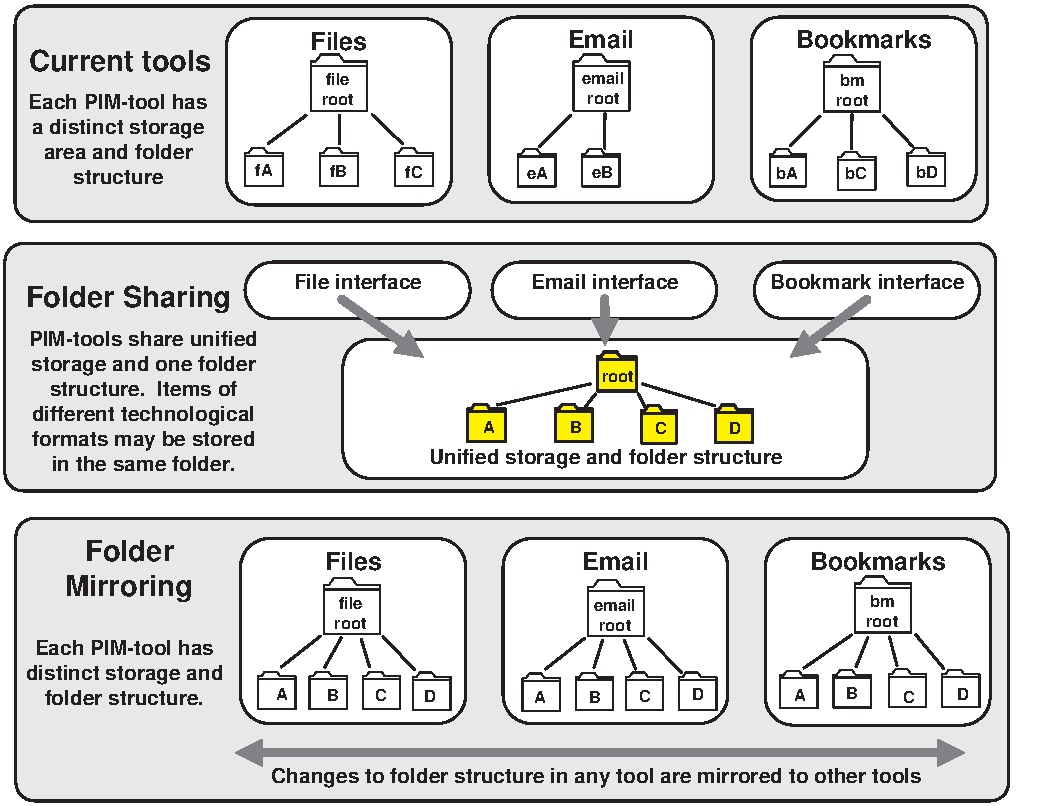
\includegraphics[height=9cm]{pictures/design/Design-fs-fm-comparison.pdf}
		% fs-fm-comparison.pdf}
	\end{center}
	\caption{Comparison of folder-sharing and folder-mirroring}
	\label{fig:design:fs-fm-comparison}
\end{figure}






%%%%%%%%%%%%%%%%%%%%%%%%%%%%%%%%%%%%%%%%%%%%%%%%%%%%%%%%%%%%%%%%%%%%%%%%%%%%%%%%%%
%%%%%%%%%%%%%%%%%%%%%%%%%%%%%%%%%%%%%%%%%%%%%%%%%%%%%%%%%%%%%%%%%%%%%%%%%%%%%%%%%%
%%%%%%%%%%%%%%%%%%%%%%%%%%%%%%%%%%%%%%%%%%%%%%%%%%%%%%%%%%%%%%%%%%%%%%%%%%%%%%%%%%
%%%%%%%%%%%%%%%%%%%%%%%%%%%%%%%%%%%%%%%%%%%%%%%%%%%%%%%%%%%%%%%%%%%%%%%%%%%%%%%%%%






%%%%%%%%%%%%%%%%%%%%%%%%%%%%%%%%%%%%%%%%%%%%%%%%%%%%%%%%%%%%%
\newpage
\section{Design Focus: Folder mirroring}
\label{design:sharing-mirroring}
%%%%%%%%%%%%%%%%%%%%%%%%%%%%%%%%%%%%%%%%%%%%%%%%%%%%%%%%%%%%%
% Can I explain in terms of psychological claims, grounded in basic-science theories, common sense argumentation 
%%%%%%%%%%%%%%%%%%%%%%%%%%%%%%%%%%%%%%%%%%%%%%%%%%%%%%%%%%%%%
% Motivation: consider different types of user?
%%%%%%%%%%%%%%%%%%%%%%%%%%%%%%%%%%%%%%%%%%%%%%%%%%%%%%%%%%%%%
This section describes the design focus in the thesis, the principle of \textit{folder-mirroring} -- allowing the user to replicate changes made to the folder structure in one tool to the folder structures in other tools. \textbf{Section~\ref{design:mirroring:evidence}} presents the empirical and methodological design rationale behind this focus.
% \textbf{Section~\ref{design:mirroring:options}} presents the initial design options that were considered.
\textbf{Section~\ref{design:core-functionality}} describes the core functionality of folder-mirroring in terms of changes to the interaction model of the standard folder hierarchy.
% Then \textbf{Section~\ref{design:rationale}} summarises the key methodological rationale behind this design focus. 

%%%%%%%%%%%%%%%%%%%
% KEY DECISION
%%%%%%%%%%%%%%%%%%%
% This decision is considered as a first focus within the initial design space.  Then a specialization of folder sharing, folder mirroring is presented.
% Folder-sharing is contrasted with related prototypes to date.

%%%%%%%%%%%%%%%
% CORE IDEA
% Present as a cross-tool design -- trying to improve cross-tool support for PIM. Theoretical interest.
%%%%%%%%%%%%%%%

%%%%%%%%%%%%%%%%%%%%%%%%%%%%%%%%%%%%%%%%%%%%%%%%%%%%%%%%%%
\subsection{Design Rationale}
\label{design:mirroring:evidence}
%%%%%%%%%%%%%%%%%%%%%%%%%%%%%%%%%%%%%%%%%%%%%%%%%%%%%%%%%%

%%%%%%%%%%%%%%%%%%
% FROM WM REPORT
%%%%%%%%%%%%%%%%%%
%The qualitative analysis of results revealed a wide range of findings related to the management of multiple hierarchies and the generation of user-defined categories (e.g. folder labels). These can be summarised as follows:
%
% The observation that users generate similar organizational categories in the form of folder labels in different tools within their workspace was a significant step in my thesis work. In other words certain folder names carry meaning across different parts of their workspace. In other words, for some users the outcome of ad-hoc parallel management of personal information is a significant amount of category overlap. In fact some users exerted significant effort towards manually synchronizing the hierarchies.
%
% It confirms that high-level user activities often involve the use of multiple tools, and suggests that many users would welcome the ability to share categories between tools.
%
% The development of WorkspaceMirror was driven by these observations and is intended to act as an evaluation platform for the hypothesis that a significant number of users would benefit from the sharing of hierarchical structure between PIM tools, and the resulting simplification of their workspace.

The next two sections present the empirical and methodological rationale behind the design focus.

%%%%%%%%%%%%%%%%%%%%%%%%%%%%%%%%%%%%%%%%%%%%%%
\subsubsection{Empirical Design Rationale}
%%%%%%%%%%%%%%%%%%%%%%%%%%%%%%%%%%%%%%%%%%%%%%

A number of findings from the exploratory study in \textbf{Chapter~\ref{chapter:exploratory_study}} lead the author to consider the potential benefits for users if they were able to share organizational structure between PIM tools.  Key findings offering evidence in favour of this design route are listed as follows:

%%%%%%%%%%%%%%%%%%%%%%%%
% Motivating factors: Empirical evidence
%%%%%%%%%%%%%%%%%%%%%%%
% laying the groundwork
% Empirical evidence that folder-mirroring may be useful is discussed. 
%%%%%%%%%%%%%%%%%%%%%%%%%%%%%%%%%%%%%%%%%%%%
% BUT: must consider ANGELA'S CLIFF!!!
% why WorkspaceMirror? Why the leap towards integrating the hierarchies?}}
%%%%%%%%%%%%%%%%%%%%%%%%%%%%%%%%%%%%%%%%%%%%
% ALSO: relate to aims (see below)
% %%%%%%%%%%%%%%%
% incremental
% pragmatic
% grounded
% simplifying
%%%%%%%%%%%%%%%%%%%%%%%%%%%%%%%%%%%%%%%%%%%
\begin{enumerate}
%%%%%%%%%%%%%%%%%%%%%%%%%%%%%%%%%%%%%%%%%%%%%%%%%%%%%%%%%%%%%
% Objective evidence: folder overlap (defendable basis?)
%%%%%%%%%%%%%%%%%%%%%%%%%%%%%%%%%%%%%%%%%%%%%%%%%%%%%%%%%%%%%
% Self-obs of overlap
%%%%%%%%%%%%%%%%%%%%%%%%%%%%
% The most common similarity was between files and email (seven participants), e.g. \textit{P1: ``Some structure is overlapping between files and email, my main activities like research and lecturing''}.  However, typically they noted that overlap was partial, often relating to primary roles.  Sometimes folders were sometimes tool-specific, e.g. \textit{P13: `` They [the email folders] are fairly close to the file system, but with some differences. For example this folder contains correspondence-based information which does not make sense in the file system''}.  Overall, many users indicated that PIM-tools shared many folders in common.  This was despite that the fact that each set of user-defined categories was developed separately as a result of compartmentalisation. 
%%%%%%%%%%%%%%%%%%%%%%%%%%%%%%%%%%%%%%%%%%%%%%%%%%%%%%%%%%%%%
%�	For those users who chose to manage more than one folder hierarchy (19 out of 21 of the participants), a significant level of overlap was noted in terms of the categories used to label folders (Boardman 2001a, 2001c.) For some users, the overlap between their file and email hierarchies was as high as 36%. 
%�	Overlapping folders tended to be based on roles, projects and interests (2001b.)
%%%%%%%%%%%%%%%%%%%%%%%%%%%%%%%%%%%%%%%%%%%%%%%%%%%%%%%%%%%%%
\item \textit{Observations of existing folder overlap between different PIM-tools} -- Firstly, the observation of substantial \textit{folder overlap} for many participants, indicated that many users who perform filing in multiple PIM-tools, create similar folders in different tool contexts (see \textbf{Section~\ref{exp-study:Results-folder-overlap}}). Furthermore, during the guided tours, eleven participants highlighted similarities between their folder structures in different tools. Folder overlap suggests that certain user activities are cross-tool and involve the organization of multiple types of information. However, with current tools, each type of information must be organized separately.  Such cross-tool activities therefore involve organizing effort that is distributed: (1) across tools, and (2) over time.

%%%%%%%%%%%%%%%%%%%%%%%%%%%%%%%%%%%%%%%%%%%%%%%%%%%%%%%%%%%%%%%%
% User comments: desire for cross-tool organization support
%%%%%%%%%%%%%%%%%%%%%%%%%%%%%%%%%%%%%%%%%%%%%%%%%%%%%%%%%%%%%%%%
% �	All the subjects emphasised the effort involved in managing multiple types of information in parallel. Note that although the study participants were technically experienced, it can be assumed that these overheads are relevant to all types of user.
% such functionality (e.g. the ability to manage files and email together) was not already provided. 
% Comments: Why do I have to manage files/email etc. separately? Empirical evidence. Quotes.
% participants encountered difficulties whilst managing multiple distinct folder hierarchies. 
% \item As well as folder overlap, other findings suggested that many users may benefit from folder-mirroring.  
\item \textit{Users expressing the wish to share folder structures between tools} -- Several participants complained about the effort of managing multiple collections of personal information separately, and expressed annoyance that it was not possible to manage their files and email together in the same set of folders, e.g.  \textit{P25: ``I suppose not as they've got very distinct usages and purposes but to me it would be easy if I could have everything in one location. But at the moment I have the sense that things are managed in two quite separate ways''}.  % \textit{Although folder-mirroring does not offer such advanced functionality, it does take steps towards this level of integration.}

%%%%%%%%%%%%%%%%%%%%%%%%%%%%%%%%%%%%%%%%%%%%%%%
% Observations of behaviour: manual mirroring
%%%%%%%%%%%%%%%%%%%%%%%%%%%%%%%%%%%%%%%%%%%%%%%
\item \textit{Manual mirroring behaviour} -- Some participants had attempted to manually mirror folders between tools.  These participants reported that it was hard to keep folder structures synchronized, and they tended to diverge over time, \textit{P13: ``All of them [my folder structures] started off with an identical folder structure, but over time they've diverged somewhat''}.  Therefore most had abandoned manual folder-mirroring because of the amount of effort involved, e.g. \textit{P11: ``I maintained my usability knowledge base for 6 months but it was too much hassle and I got out of practice. I want to get restarted in email, file system and web''}.
% They also stated that they tried to keep them in sync, or that they started off in sync, but that it was too much hassle to do manually over time. 
%One participant saved multiple types of information within one folder structure.  She saved email messages as word documents within her file system rather than have to manage another set of folders.
These observations suggested that some users may welcome folder-mirroring. 

%%%%%%%%%%%%%%%%%%%%%%
% Easier retrieval
%%%%%%%%%%%%%%%%%%%%%%
% It was envisaged that consistent organization may also help the user retrieve more effectively.
\item \textit{Difficulties in retrieving information} -- Some participants mentioned problems when retrieving information caused by them not being sure if it was stored in the file collection or the email collection. In particular, retrieval problems were caused by the ability to manage files as attachments within the email collection, e.g. \textit{P22: ``If it wasn't there [in the file folder] I would think damn I forgot to file it in the folder where it belongs and go straight to email''}.  Retrieval problems may be exacerbated by the existence of different organizational structures in each tool. This means that as well as looking in two tools, users may have to look in different locations in each tool. 
% POSSIBLE EXAMPLES files in X, email in Y

\end{enumerate}

%%%%%%%%%%%%%%%%%%%%
% FROM WM REPORT
%%%%%%%%%%%%%%%%%%%%
% The observation that users generate similar organizational categories in the form of folder labels in different tools within their workspace was a significant step in my thesis work. In other words certain folder names carry meaning across different parts of their workspace. In other words, for some users the outcome of ad-hoc parallel management of personal information is a significant amount of folder overlap. 
%
% It confirms that high-level user activities often involve the use of multiple tools, and suggests that many users would welcome the ability to share categories between tools.
%
% The development of WorkspaceMirror was driven by these observations and is intended to act as an evaluation platform for the hypothesis that a significant number of users would benefit from the sharing of hierarchical structure between PIM tools, and the resulting simplification of their workspace.

%%%%%%%%%%%%%%%%%%%%%%%%%%%%%%%%%%%%%%%
% Also consider CONTRASTING counter-arguments
%%%%%%%%%%%%%%%%%%%%%%%%%%%%%%%%%%%%%%%
% Although there was a large amount of evidence in favour of folder-sharing, the author was also aware that there were also counter-arguments.  
The exploratory study also provided evidence that folder-mirroring may \textit{not} be useful.  Folder overlap was in many cases partial, and often limited to certain types of folders such as roles and projects.  In other words, there was some variation in organizational behaviour across the three tools for many participants.
% ADD INTO CHAPTER 4).
Furthermore, some users did not rely on folders and instead relied on sort and search mechanisms.  Therefore would stand to gain little benefit from folder-mirroring.
% Firstly, as noted above, some users stated that they required the flexibility to organize different types of information in different ways -- something which would be inhibited if one set of folders were shared across collections. 

%%%%%%%%%%%%%%%%%%%%%%%%%%%%%%%%%%%%%%%%%%%%%%%%
% Bottom line: interesting area to look at
%%%%%%%%%%%%%%%%%%%%%%%%%%%%%%%%%%%%%%%%%%%%%%%%
%%%%%%%%%%%%%%%%%%%%%%%%%%%%%%
% Empirical investigation
% Interest: do (which?) users do not need different classification schemes for different types of information.
% A key trade-off is identified between PIM overheads and flexibility. % Can this trade-off be expressed in terms of psychological claims along the lines of Carroll? A key sub-issue is identified: how does this trade-off vary between users? 
% Possible Design trade-offs, e.g. overheads versus flexibility. Types of flexibility.
% Real aim: design as test-bed/straw-man -- to explore potential to unify/integrate.
% Explore trade-off's inherent in design (REF: Carroll)
%%%%%%%%%%%%%%%%%%%%%%%%%%%%%%
% Test case/test-bed for/develop methodology, research vehicle to investigate potential to improve integration
% how would users receive the ability to share organizational structure between tools? 
The two sides of this argument indicated that this was be an interesting area to investigate further.  
An implementation of folder-mirroring was envisaged as a research vehicle to investigate the potential of increased integration. The following issues were identified for exploration: how would users respond to the ability to share folders between tools?  Do folder labels carry meaning beyond the boundaries of particular tools?  Do users really need the flexibility to develop distinct classification schemes for different types of personal information? 

%%%%%%%%%%%%%%%%%%%%%%%%%%
% Design hypothesis
%%%%%%%%%%%%%%%%%%%%%%%%%%
% some kind of automatic mechanism could help fulfil this need.  Intuitive need (users need it?), not done manually (too much hassle).  Add similarity of strategies.
The subsequent implementation and evaluation of a folder-mirroring prototype was directed at investigating whether the folder-mirroring mechanism would help users manage the multiple types of information relating to certain activities more effectively.
%%%%%%%%%%%%%%%%%%%%%%%%%
% Speculation: predicted behaviour: Converge over time

%%%%%%%%%%%%%%%%%%%%%%%%%
%%%%%%%%%%%%%%%%%%%%%%%%%%%%%%%%%%%%%%%%%%%%%%%%%%%%%%
% CURRENT: different PIM-tools, manage separately
%%%%%%%%%%%%%%%%%%%%%%%%%%%%%%%%%%%%%%%%%%%%%%%%%%%%%%
% a user can make adjustments to the folder structures in different PIM-tools as required.
In the personal information environment offered by current desktop computers, users must make adjustments separately to the folder structures in different PIM-tools.  Since the folder structures are managed separately, even if users try to keep them synchronized, they tend to diverge over time.  % THINK: would they do this anyway?
With folder-mirroring, it was envisaged that the folder-structures in different collections of personal information may converge.


%%%%%%%%%%%%%%%%%%%%%%%%%%%%%%%%%%%%%%%%%%%%%%%%%%%%%%%%%%
% PERSONAL: Most promising of the prototypes?
% Based on initial feedback from prospective users?
%%%%%%%%%%%%%%%%%%%%%%%%%%%%%%%%%%%%%%%%%%%%%%%%%%%%%%%%%%
% \item As well as relating to an interesting area to study, the author considered this the most promising of the potential designs outlined in \textbf{Section~\ref{design:initial-forays}}.



%%%%%%%%%%%%%%%%%%%%%%%%%%%%%%%%%%%%%%%%%%%%%%%%%%%%%%%%%%
% \subsection{Design rationale}
% \label{design:rationale}
%%%%%%%%%%%%%%%%%%%%%%%%%%%%%%%%%%%%%%%%%%%%%%%%%%%%%%%%%%
% Discuss benefits OVER and BEYOND folder-sharing
% Folder-mirroring retains many of potential benefits of folder-sharing whilst also providing flexibility.
%%%%%%%%%%%%%%%%%%%%%%%%%%%%%%%%%%%%%%%%%%%%%%%%%%%%%%%%%%




%%%%%%%%%%%%%%%%%%%%%%%%%%%%%%%%%%%%%%%%%%%%%%
\subsubsection{Methodological Design Rationale}
%%%%%%%%%%%%%%%%%%%%%%%%%%%%%%%%%%%%%%%%%%%%%%

%%%%%%%%%%%%%%%%%%%%%%%%%%%%%%%%%%%%%%%%%%%%%%%%%%%%%%%%%%
% KEY DESIGN AIM: Incremental
% facilitate up-take of system and effective evaluation
%%%%%%%%%%%%%%%%%%%%%%%%%%%%%%%%%%%%%%%%%%%%%%%%%%%%%%%%%%
% In this section the methodological rationale for this design focus are discussed.
% The focus on folder-mirroring was made for the following reasons:
% Folder-mirroring offers an incremental change relative to current systems. Therefore the design route offers the potential benefits of evolutionary ``hill-climbing'' outlined in \textbf{Section~\ref{design:aims}}.
Folder-mirroring was also seen to be highly compatible with an evolutionary, incremental design route:

\begin{enumerate}

%%%%%%%%%%%%%%%%%%%%%%%%%%%%%%%%%%%%%%%%%%%%%%%%%%%%%%%%%%
% Incremental consequence 2: Few usage barriers
%%%%%%%%%%%%%%%%%%%%%%%%%%%%%%%%%%%%%%%%%%%%%%%%%%%%%%%%%%
\item It was envisaged that folder-mirroring functionality could be applied to existing folder structures, which would be extended incrementally with mirrored folders.  Therefore there are few barriers to initial usage since the user does not have to adjust existing collections in any way. Furthermore, folder-mirroring could be made optional, allowing users to retain the flexibility to organize different types of information in different ways. % i.e.take step towards unification but flexibility is retained.

%%%%%%%%%%%%%%%%%%%%%%%%%%%%%%%%%%%%%%%%%%%%%%%%%%%%%%%%%%
% Incremental consequence 1: Practical/pragmatic route
%%%%%%%%%%%%%%%%%%%%%%%%%%%%%%%%%%%%%%%%%%%%%%%%%%%%%%%%%%
% Step towards PIM-unification in more ambitious schemes - therefore achievable?
% , external constraints -- therefore choice of incremental step, \textit{do-able
%  potential to complete the cycle}
%%%%%%%%%%%%%%%%%%%%%%%%%%%%%%%%%%%%%%
\item Folder-mirroring can be considered a step towards the PIM-integration offered in systems such as MS-WinFS~\citep{winfs:03}.  It was envisaged that this design route represented a practical/pragmatic choice, achievable within the limited time and manpower constraints available, that would provide insight for the developers of more advanced PIM-integration technology.  Based on the author's previous technical experience, it was estimated that the folder-mirroring principle would be possible to implement in a robust way with the limited available time and manpower resources.

%%%%%%%%%%%%%%%%%%%%%%%%%%%%%%%%%%%%%%%%%%%%%%%%%%%%%%%%%%
% KEY DESIGN AIM: EXTENSIBLE
% Lays foundation for more powerful functionality
%%%%%%%%%%%%%%%%%%%%%%%%%%%%%%%%%%%%%%%%%%%%%%%%%%%%%%%%%%
% Longer-term design argument: facilitate project management/knowledge transfer functions
% Folder-mirroring is extendible - it can be built on to provide further PIM integration.
\item Sharing one set of folders across PIM-tools would act as a foundation for more powerful PIM functionality. For example, organizational consistency in this way facilitates the straightforward grouping of related information in different technological formats. Envisaged uses for such cross-tool grouping include collating information for knowledge transfer, starting a new project, or project archiving.
% (``Bill needs to pass on project X to Jane'')
% (``Bill wants to start a new project and wants to create a folder in all his PIM-tools associated with that project'')
% (``Bill is finishing Project X, and wants to archive all related information'')
% A number of design suggestions were received from users in the evaluations reported in \textbf{Section~\ref{design:feasibility-study}} and \textbf{Chapter~\ref{chapter:main-study}}. However in the bulk of the thesis, only the core folder-mirroring functionality is considered.
% Example design steps are outlined (discussed in \textbf{Section~\ref{design:design-extensions}} below, and also under further work in \textbf{Chapter~\ref{chapter:conclusion}}). 

\end{enumerate}









%%%%%%%%%%%%%%%%%%%%%%%%%%%%%%%%%%
\subsection{Core Functionality}
\label{design:core-functionality}
%%%%%%%%%%%%%%%%%%%%%%%%%%%%%%%%%%

%%%%%%%%%%%%%%%%%%%%
% FROM WM REPORT
%%%%%%%%%%%%%%%%%%%%
% The software synchronizes three folder hierarchies: the user's "home directory" where personal documents are stored; (2) web bookmarks stored in the "Favorites" folder; and (3) email messages stored in Microsoft Outlook. WE expect that the software will reduce management overheads, and improve integration for many users - although at the expense of the flexibility to organize different types of information in different ways.

%%%%%%%%%%%%%%%%%%%%%%
% DESCRIBE DESIGN
%%%%%%%%%%%%%%%%%%%%%%
% Discuss as reducing organizational redundancy. Attempt to leverage investment that user is willing to make in structuring their workspace beyond particular tools (promotion of consistency, coherency, positive constraint on user).
% Leverage investment -- support of satisficing. Help users stay organized with less effort (if they want to) and manage the different types of information that they collect in various tools around their workspace. Promote consistency/coherency
%%%%%%%%%%%%%%%%%%%%%%%%%%%%%%%%%%%%%%%%%%%%%%%%%%%%%%%%%%%%%%%%%%%%%%
%	system model to (formally?) describe system}
%	Scenarios are presented to illustrate example situations in which folder-sharing could be used (i.e. confirm the concern/requirement/user need that is the object of design). 
%%%%%%%%%%%%%%%%%%%%%%%%%%%%%%%%%%%%%%%%%%%%%%%%%%%%%%%%%%%%%%%%%%%%%%
% Interface dialogue-level description -- user interaction model
%		\item Relate to the different aspects of PIM
%		\item Scenarios, screen-shots and storyboards
%		\item NB: Not trying to deal with inherent limitations of the hierarchy
%%%%%%%%%%%%%%%%%%%%%%%%%%%%%%%%%%%%%%%%%%%%%%%%%%%%%%%%%%%%%%%%%%%%%%
In this section, the folder-mirroring design is outlined in detail. Firstly,the interactions afforded by the  traditional folder hierarchy are described in terms of three fundamental operations:
%%%%%%%%%%%%%%%%%%%%%%%%%%%%%%%%%%%%%%%%%%%%%%%%
% Functionality of existing folder structures
%%%%%%%%%%%%%%%%%%%%%%%%%%%%%%%%%%%%%%%%%%%%%%%%
% Add a folder
% Delete a folder
% Rename a folder
% THINK: move to folder mirroring?
% The traditional folder hierarchy allows 
\begin{enumerate}
\item \textit{Creating a new folder} -- The folder's location within the folder structure, is defined by the folder's path relative to the root folder. % (e.g. creating folder \texttt{Marylebone} at location \texttt{Root/Train-stations}.
\item \textit{Deleting a folder} -- Items and sub-folders contained within the folder are also deleted.
\item \textit{Renaming a folder} -- In the simplest case, a folder's name is changed, but the folder remains at the same location.  \textit{Moving} a folder can be considered a special case of renaming where the folder's path is changed but the name remains the same.
\end{enumerate}



%%%%%%%%%%%%%%%%%%%%%%%%%%%
% Desired CORE functionality
% Outline interaction model and options thereof. 
% When the user does X, WM offers Y. Scenarios through the functionality.
% Retain 3 different folder structures, but mirror changes between them
% Improve reference to diagram
%%%%%%%%%%%%%%%%%%%%%%%%%%%
The folder-mirroring principle allows the user to replicate the three above operations across multiple folder structures as shown in \textbf{Figure~\ref{fig:design:mirroring}}.  In other words, if a change is made made to the folder structure in one collection, it is replicated to the folder structures in the other collections. % supported by the mechanism.

The core functionality of folder-mirroring, can be defined as follows, in terms of the three above operations: % NB: this is automatic mirroring
\begin{enumerate}

\item \textit{Mirroring the creation of a folder} -- If the user adds a new folder ``C'' in one collection, an equivalent folder ``C'' should be created in the same location in the other collections.  If a folder with that name already exists in that location in one of the other collections, no action should be taken there.

It may be necessary to mirror an entire set of parent folders as follows. Consider the scenario of a folder being mirrored from the file system to email. The file folder in question is \texttt{File-root/A/B}. In email, the intermediate folder, \texttt{Email-root/A} does not exist.  Therefore, the parent folder, \texttt{Email-root/A} must be created before \texttt{B} is created.

\item \textit{Mirroring the deletion of a folder} -- When the user deletes a folder ``C'' in one collection, the equivalent folder (if one exists) should be deleted in the other collections.  If that folder does not exist in one of the other collections, no action should be taken there.

\item \textit{Mirroring the renaming of a folder} -- A scenario is considered when the user renames a folder ``B'' (termed the \textit{source folder}) as folder ``C'' (termed the \textit{destination folder}).  If the source folder exists in one of the other collections at that same location, \textit{and} if the destination folder does not exist, then renaming should be mirrored.  If the source folder does not exist, or the destination already exists in a particular collection, then no action should be taken there\footnote{An alternate design was also considered for renaming, in the case when the source \textit{and} destination folders do not exist in another PIM-tool.  Instead of the action detailed above, the destination folder could be created in the other PIM-tool, and so make the folder structures more consistent.  This alternate design was not implemented in the course of the thesis but remains a possibility for future work.}.
\end{enumerate}

% Examples of the three mirroring operations are shown in \textbf{Figure~\ref{fig:design:mirroring}}.
% %%%%%%%%%%%%%%%%%%%%%%%%%%%%%
% FIGURE - Principles of Mirroring
% %%%%%%%%%%%%%%%%%%%%%%%%%%%%%
%%%%%%%%%%%%%%%%%%%%%%%%%%%%%%%
\begin{figure}[htb]
	\begin{center}
		\leavevmode
		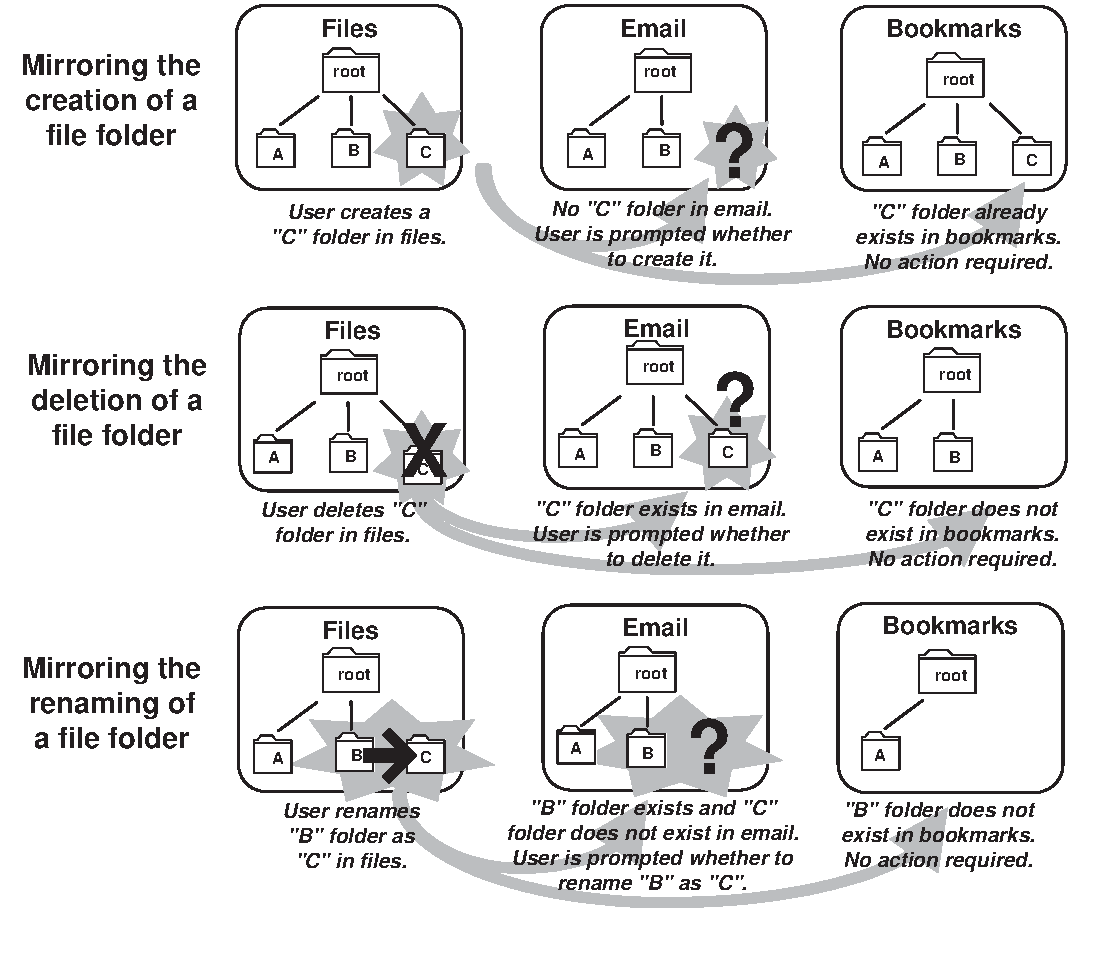
\includegraphics[width=.9 \textwidth]{pictures/design/Design-mirroring.pdf}
	\end{center}
	\caption{Principles of mirroring}
	\label{fig:design:mirroring}
\end{figure}


%%%%%%%%%%%%%%%%%%
% Suitable tools
%%%%%%%%%%%%%%%%%%
The file, email and bookmark collections were deemed suitable for folder-mirroring since they all employ hierarchy-based organizations to arrange items.  Other PIM-tools such as the calendar and contact manager are not suitable because in most cases they do not rely on hierarchical organization\footnote{One can envisage the sharing of folder labels between hierarchy-based tools such as email, and non-hierarchy-based tools such as calendars.  However, this functionality was beyond the scope of the work in this thesis.}.
%%%%%%%%%%%%%
% 2 modes
%%%%%%%%%%%%%
Two modes of operation were envisaged: \textit{automatic} and \textit{manual}. In the automatic mode, folder actions are mirrored automatically. In the manual mode, the user is prompted with a dialogue box as to whether mirroring should be performed.

%%%%%%%%%%%%%%%%%%
% Discussion: NOT ABOUT AN ALTERNATIVE TO THE FOLDER
% Assumption: keep folders.
%%%%%%%%%%%%%%%%%%
% The specific problem being investigated is the current fragmentation between different tools. 
Note that folder-mirroring should not be considered as an attempt to develop an alternative to hierarchical organization.   Limitations of the hierarchy such as single-inheritance~\citep{dourish:99a} are beyond the scope of the thesis.
% The fact is outlined that folder-mirroring is not targeted at providing alternative to the hierarchy.
% Encourage good habits? (risky)
%%%%%%%%%%%%%%%%%%%%%%%%%%%%%%%%%%%%%%%%%%%%%%%%%%%%%%%%%%%%%%%%%%%%%%%%%
% Also, not concerned with providing alternative interaction techniques
%%%%%%%%%%%%%%%%%%%%%%%%%%%%%%%%%%%%%%%%%%%%%%%%%%%%%%%%%%%%%%%%%%%%%%%%%
Also, it should also be noted that folder-mirroring does not provide an alternative means for interacting with folder structures. The user interacts with the three PIM-tools as before (e.g. via direct manipulation, or the command-line).

%%%%%%%%%%%%%%%%%%%%%%%%%%%%%%%%%
\subsubsection{Usage Scenarios}
\label{design:mirroring:scenarios}
%%%%%%%%%%%%%%%%%%%%%%%%%%%%%%%%%

%%%%%%%%%%%%%%
% Scenarios
%  (i.e. confirm the concern/requirement/user need that is the object of design):
%%%%%%%%%%%%%%
Two scenarios were developed, based on comments from the exploratory study, to illustrate how folder-mirroring could be used:
\begin{itemize}

%%%%%%%%%%%%%%%%%%%%%%%
% Creation example
%%%%%%%%%%%%%%%%%%%%%%%
\item \textit{Starting a project} -- Bill is about to embark on a new coding project.  The project involves creating source code and documentation, coordinating with colleagues, and researching information on the internet.  Therefore he predicts that the project will involve the management of associated files, email and bookmarks.
%\begin{enumerate}
%	\item \textit{Create file folder} -- Bill selects his file management tool, navigates to the desired location in the file system, creates the folder, and names it
%	\item \textit{ Create email folder} -- repeat actions as for file folder
%	\item \textit{Create web bookmark folder} -- repeat actions as for file folder
%\end{enumerate}

% Note that in many cases, these actions would not happen sequentially.  PIM is interleaved with the other activities involved in Bill's work, many of which take precedence over PIM.  In fact most users do not have time to manually organize multiple hierarchies, even if they want to. Note also that the sets of actions, if they happen, could happen in any order. Note also that each folder may be located in a different location in the relevant hierarchy.
Using current tools, Bill must create folders separately in each tool in turn.  However, with folder-mirroring, Bill can create a project folder in one location and is then immediately prompted as to whether he wants the folder also created in the other locations. He decides to mirror and the folder is created in the three tool contexts.

%%%%%%%%%%%%%%%%%%%%%%
% Deletion example
%%%%%%%%%%%%%%%%%%%%%%
% Jenny finishes working on "Project Y", after six months working on it flat-out and it being a bane on her life, she doesn't want anything else to do with it. And as one small step towards that she would like it to delete it from her workspace.
% Currently - yet again, three separate sets of actions must be carried out:
%1.	Delete folder in document context
%a.	execute corresponding sub-activities ...
%2.	Delete folder in email context
%a.	execute corresponding sub-activities ...
%3.	Delete folder in web bookmark context.
%a.	execute corresponding sub-activities ...
%
%With WorkspaceMirror Mary would navigate to any PIM tool and delete the folder, after which it would be automatically deleted in the other tools:
%a)	Select a PIM tool (unless user is already there)
%b)	Navigate to desired location in folder hierarchy
%c)	Select "Project Y" and delete it  
%d)	A dialog window appears, asking the user if they also want to delete the folder in the other PIM contexts .
%e)	Transparently the equivalent folders are deleted in the other PIM tools, making use of Recycle Bin facilities where appropriate.
\item \textit{Finishing a project} --  Gemma has just completed a term report on the mating habits of hamsters.  Whilst carrying out this activity, she has managed a large amount of associated files, email and bookmarks within a \texttt{hamster} folder in the respective PIM-tools.  Having backed up the term report itself, Gemma wants to delete all the information relating to the report which are cluttering up her workspace.

Using current tools, she must go to each tool in turn and delete the respective folders and the items they contain.  With folder-mirroring, she is prompted to delete the folder in all three tools, thus saving mouse-clicks and time.  The scenarios assumes that she had previously created the folder in each tool\footnote{Note that an equivalent cross-tool archiving function can also be imagined as an alternative to the cross-tool deletion portrayed in this scenario.}.


%%%%%%%%%%%%%%%%%%%%%
% renaming example
%%%%%%%%%%%%%%%%%%%%%
%Currently Mary also manages each type of personal information separately in distinct tools. Any reorganization must be done performed manually in each tool. Mary currently organizes her work based on project: "Project A", "Project B", "Project C" and so on. Each project is represented by a top-level folder in each of her PIM tools. However on realizing that "Project Z" and "Project A" are both related to one customer "FGH Ltd.", she decides to make this explicit in her workspace. " FGH Ltd." is also represented by a top-level folder in each PIM tool.
%
%Mary must perform three separate sets of actions in three separate tools:
%1.	Move Document folders
%a.	Select document management tool (unless user is already there)
%b.	Navigate to top level in document hierarchy (the file system)
%c.	Select "Project A" and move it into "FGH Ltd.".  
%d.	Repeat for "Project Z"
%2.	Move Email folders
%a.	Select email management tool
%b.	Navigate to top level in email folder hierarchy
%c.	Select "Project A" and move it into "FGH Ltd.".  
%d.	Repeat for "Project Z"
%3.	Move Web Bookmark folders
%a.	Select web bookmark management tool
%b.	Navigate to top level in web bookmark hierarchy
%c.	Select "Project A" and move it into "FGH Ltd.".  
%d.	Repeat for "Project Z"
%
%As before, the interleaved, ad-hoc nature of PIM means that these actions could happen in any order, and few users could be bothered to be so organized.
%
%With WorkspaceMirror Mary would navigate to any PIM tool and carry out her reorganization, after which it would be mirrored in the other tools:
%1.	Move folders in any PIM context
%a)	Select a PIM tool (unless user is already there)
%b)	Navigate to desired location in folder hierarchy
%c)	Select "Project A" and move it into "FGH Ltd.".  
%d)	A dialog window appears, asking the user if they also want to move the folder in the other PIM contexts .
%e)	Transparently the equivalent folders are moved in the other PIM tools.
%f)	Repeat for "Project Z"

\end{itemize}


%%%%%%%%%%%%%%%%%%%%%%%%%%%%%%%%%%%%%%%%%%%%%%%%%%%%%%%%%%%%%%%%%%%%%%%%%%%%%%%%%%
%%%%%%%%%%%%%%%%%%%%%%%%%%%%%%%%%%%%%%%%%%%%%%%%%%%%%%%%%%%%%%%%%%%%%%%%%%%%%%%%%%
%%%%%%%%%%%%%%%%%%%%%%%%%%%%%%%%%%%%%%%%%%%%%%%%%%%%%%%%%%%%%%%%%%%%%%%%%%%%%%%%%%
%%%%%%%%%%%%%%%%%%%%%%%%%%%%%%%%%%%%%%%%%%%%%%%%%%%%%%%%%%%%%%%%%%%%%%%%%%%%%%%%%%




%%%%%%%%%%%%%%%%%%%%%%%%%%%%%%%%%%%%%%%%%%%%%%%%%%%%%%%%%%
%%%%%%%%%%%%%%%%%%%%%%%%%%%%%%%%%%%%%%%%%%%%%%%%%%%%%%%%%%
\newpage
\section{Prototype Implementation}
\label{design:wm-prototyping}
%%%%%%%%%%%%%%%%%%%%%%%%%%%%%%%%%%%%%%%%%%%%%%%%%%%%%%%%%%
%%%%%%%%%%%%%%%%%%%%%%%%%%%%%%%%%%%%%%%%%%%%%%%%%%%%%%%%%%
% WorkspaceMirror: a PIM-unification prototype % based on folder mirroring}
% Add to discussion:

%%%%%%%%%%%%%%%%%%%%%%%%%%%%%%%%%%%%%%%%%%%%%%%%%%
%Design constraints (from core functionality):
%%%%%%%%%%%%%%%%%%%%%%%%%%%%%%%%%%%%%%%%%%%%%%%%%%
%	\item Initial design constraints: desktop workspace
%	\item The decision was taken to mirror folders between three tools - the file system, email and web bookmarks.
%	\item Extension of standard tools -- for familiarity

%%%%%%%%%%%%%%%%%%%%%%%%%%%
% Introduce section
%%%%%%%%%%%%%%%%%%%%%%%%%%%
% Firm belief in firmware.
% Therefore next step was to prototype the design in order to explore pros versus cons.
% Focus on subset of core issues
% Key aims: robustness and long-term usability
This section describes the implementation of a folder-mirroring prototype, \textit{WorkspaceMirror} (abbreviated in this thesis as WM).
%%%%%%%%%%%%%%%%%%%%%%%%
% Choice of platform
%%%%%%%%%%%%%%%%%%%%%%%%
Development was carried out on the MS-Windows desktop operating system, using the languages MS-Visual Basic 6.0 and MS-Visual Basic.NET.  The popular MS-Windows operating system was selected so as to provide access to the largest possible number of potential users.  %Visual Basic was selected due to its status as a development tool suitable for rapid interface prototyping.  % add ~\citep{}.
% See below for reasons for 2 different versions
Rather than recounting the rounds of iterative development and testing performed by the author, a focus is taken on the final architecture of WM.  % However, key design decisions are detailed.


%%%%%%%%%%%%%%%%%%%%%%%%%%%%%%
% Implementation outline
%%%%%%%%%%%%%%%%%%%%%%%%%%%%%%
% WorkspaceMirror has been implemented under MS Windows and synchronizes changes made to the folder hierarchies in three tools: (1) email folders in MS Outlook, (2) the user's document area in the file system, and (3) bookmark folders stored under Favorites. 
WM runs as a background application, monitoring for the creation, deletion, or renaming of folders in three PIM-tools:
\begin{enumerate}

\item \textit{One user-selected area of the file collection} --  The exploratory study highlighted that users often store personal files in multiple locations such as the desktop, the local hard disk, and drives on remote servers.  It was decided to focus on one area of the file system (e.g. ``My Documents'') for two reasons: (1) to enable straightforward mirroring with the email and bookmark collections which are each centred on one primary folder structure, and (2) to enable fast implementation.

\item \textit{MS-Outlook (email collection)} -- A wide range of email clients are in common usage including MS-Outlook, Eudora, Netscape and MS-Outlook Express.  Initial investigation revealed that each client employs incompatible storage formats meaning that it was not possible to support all the clients within the limited time available.  MS-Outlook was chosen as the supported  client because: (1) it possessed a well-defined API accessible from Visual Basic, and (2) it was the most common client encountered in the exploratory study. % chosen as a common email reader with an API that was easily accessible from Visual Basic

\item \textit{MS-Internet Explorer (bookmark collection, also known as ``Favorites'')} -- MS-Internet Explorer was selected as the most common web browser on the MS-Windows platform.

\end{enumerate}

%%%%%%%%%%%%%%%%%%%%%%%%%%%%%%%%%%
% Runs in background - 2 modes
%%%%%%%%%%%%%%%%%%%%%%%%%%%%%%%%%%
WM operates in one of two modes: \textit{automatic} or \textit{prompted}. A configuration setting allows switching between the two modes. In automatic mode, events are mirrored without user intervention.  In prompted mode, WM runs in the background except for prompting the user when the user performs a folder-related operation.  The creation, deletion or renaming of any folder causes a dialogue box to be displayed asking the user if they want to replicate the operation in the other two tools.  An example dialogue box is shown in \textbf{Figure~\ref{fig:design:wm-dialogue}}.  Each of the three PIM-tools are represented by a check box, which can be selected to request mirroring to be performed in that tool. The check box corresponding to the PIM-tool which has sourced the event is hashed out.  A configuration setting allows the user to specify whether the check boxes are enabled or disabled by default. If the check boxes are enabled by default, simply pressing the 'OK' button on the dialogue box causes mirroring to proceed. 


% \textbf{Figure~\ref{fig:design:wm-dialogue}} shows a sample dialogue.
% %%%%%%%%%%%%%%%%%%%%%%%%%%%%%
% FIGURE - example dialogue
% %%%%%%%%%%%%%%%%%%%%%%%%%%%%%
%%%%%%%%%%%%%%%%%%%%%%%%%%%%%%%
\begin{figure}[htbp]
	\begin{center}
		\leavevmode
		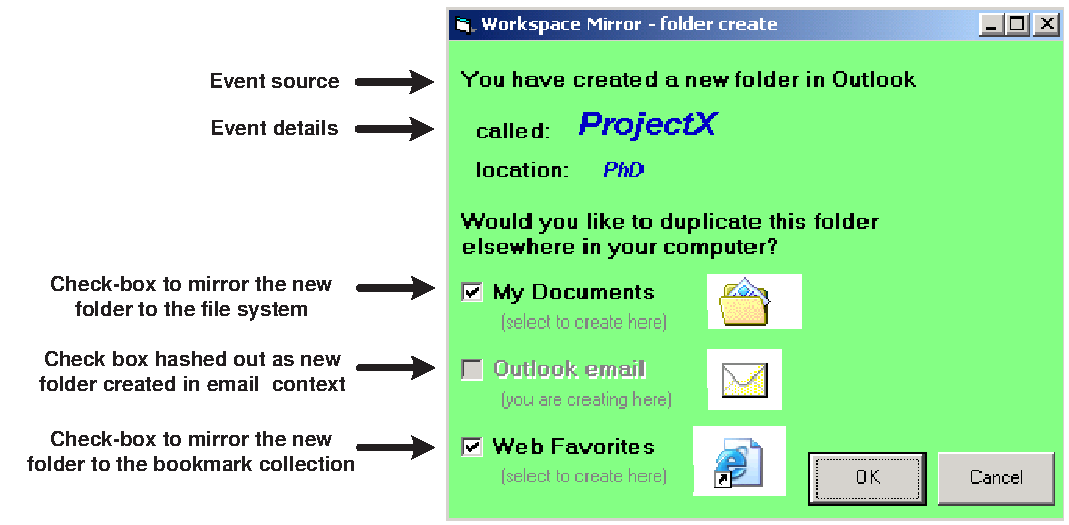
\includegraphics[width=.8 \textwidth]{pictures/design/Design-dialogue.pdf} % Design-dialogue.pdf}
	\end{center}
	\caption{Example WM dialogue: the folder \texttt{PhD/ProjectX} has been created in email.}
	\label{fig:design:wm-dialogue}
\end{figure}

% %%%%%%%%%%%%%%%%%%%%%%%
% Architecture
% %%%%%%%%%%%%%%%%%%%%%%%
\textbf{Figure~\ref{fig:design:architecture}} describes the architecture of the WM prototype, which consists of four main components: (1) \texttt{dotNetWatcher}, (2), \texttt{OutlookWatcher}, (3) \texttt{EventProcessor}, and (4) \texttt{Mirrorer}\footnote{Most of the application coding was performed in MS-Visual Basic 6.0. The only exception was the \texttt{dotNetWatcher} component which was coded in MS-Visual Basic.NET. This version was selected since it offered significantly enhanced support for file system monitoring through the \texttt{FileSystemWatcherClass} class. The \texttt{dotNetWatcher} component communicates with the other components via the ``COM/.Net interop'' mechanism. Since MS-Visual Basic.NET was a beta product at the time of development (Summer/Autumn 2002),  integration between the COM and .NET components was coded manually and was non-trivial.}.  
% \texttt{dotNetWatcher} was implemented in Visual Basic .NET, whilst Visual Basic 6.0 was used for the other three components. 

% The prototype architecture is described in \textbf{Figure~\ref{fig:design:wm-architecture}}.
% %%%%%%%%%%%%%%%%%%%%%%%%%%%%%
% FIGURE - basic architecture and event model
% %%%%%%%%%%%%%%%%%%%%%%%%%%%%%
%%%%%%%%%%%%%%%%%%%%%%%%%%%%%%%
\begin{figure}[htbp]
	\begin{center}
		\leavevmode
		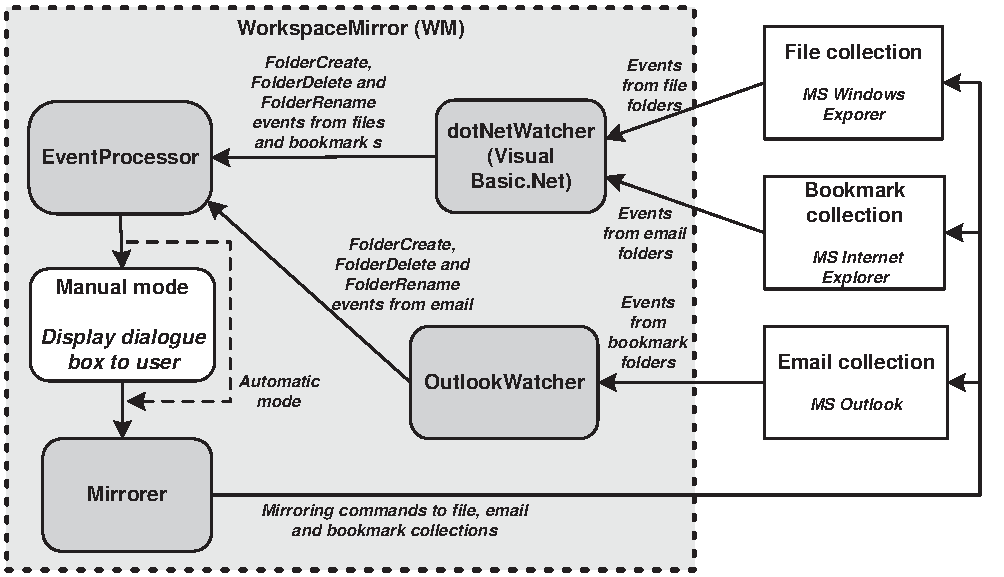
\includegraphics[width=.8 \textwidth]{pictures/design/Design-architecture.pdf}
	\end{center}
	\caption{WorkspaceMirror: overview of technical architecture}
	\label{fig:design:architecture}
\end{figure}

%%%%%%%%%%%%%%%%%%%%%%%%%%%%%%%%%%%%%%%
% dotNetWatcher and OutlookWatcher
%%%%%%%%%%%%%%%%%%%%%%%%%%%%%%%%%%%%%%%
The first two components, \texttt{dotNetWatcher} and \texttt{OutlookWatcher} monitor the three PIM-tools for folder-related events. \texttt{dotNetWatcher} monitors the portions of the file system corresponding to the user's personal files (e.g. ``My Documents''), and bookmarks (termed ``Favorites'' in MS-Windows). \texttt{OutlookWatcher} monitored the folder structure in MS-Outlook. These two components instantiate a \texttt{FolderCreate}, \texttt{FolderDelete} or \texttt{FolderRename} object containing the details of any detected creation, deletion or renaming event. For example the \texttt{FolderCreate} object contains details on the folder name, folder path, and the PIM-tool which generated the event.  All events are then relayed to the 
\texttt{EventProcessor} component.

%%%%%%%%%%%%%%%%%%%%%%
% EventProcessor
%%%%%%%%%%%%%%%%%%%%%%
% Handling recursion
% \item Deletion: avoid cascade of child folder echoes	
The \texttt{EventProcessor} component contains the main application logic for WM. 
Firstly, \texttt{EventProcessor} filters two types of spurious events which are not appropriate for mirroring.
The first type of event are those that relate to default folders (e.g. the creation of a new folder under ``Deleted items'' in email).  \texttt{EventProcessor} maintains a cache of default folders from commonly encountered applications for this purpose.  The \texttt{EventProcessor} component also handles the possibility of event recursion due to folder mirroring.  For example, consider the mirroring of a newly created folder from the file system to email.  The newly mirrored email folder causes a second \texttt{FolderCreate} event to be created, this time by the \texttt{OutlookWatcher} component. \texttt{EventProcessor} avoids event recursion by filtering new events based on a cache of previously mirrored events.   Non-filtered events are processed as follows:
\begin{itemize}

%%%%%%%%%%%%%%%%%%%%%%%%%%%%%%%%%%%%%%%%%%
% Folder creation (name X, location Y)
%%%%%%%%%%%%%%%%%%%%%%%%%%%%%%%%%%%%%%%%%%
\item \textit{FolderCreate event} -- The existence of the folder is checked in the same location in the other PIM-tools.  If there is at least one PIM-tool where there is no corresponding folder, \texttt{EventProcessor} proceeds to mirror the event.  In manual mode, a dialogue box is displayed asking the user if they want to create the folder in those PIM-tools where that folder does not already exist (see \textbf{Figure~\ref{fig:design:wm-dialogue}}).  A configuration setting specifies whether the check boxes are selected by default. Those check-boxes corresponding to the source PIM-tool, and any PIM-tools where the new folder already exists are disabled.  In automatic mode, folders are mirrored automatically as appropriate.
% \item Rebuilding parent chain for creation

%%%%%%%%%%%%%%%%%%%%%%%%%%%%%%%%%%%%%%%%%%%
% Folder deletion: name X, location Y
%%%%%%%%%%%%%%%%%%%%%%%%%%%%%%%%%%%%%%%%%%%
% this is what Cooper might call dangerous functionality.   
\item \textit{FolderDelete event} -- The existence of the folder is verified in the other PIM-tools.  If there is at least one other PIM-tool where the folder exists, \texttt{EventProcessor} proceeds to mirror the event.  In automatic mode, any equivalent folders are deleted automatically\footnote{It may be argued that such ``automatic deletion'' functionality is dangerous as it makes it too easy for the user to remove information without thinking.  Consequently, WM took full advantage of any ``Recycle Bin'' functionality so as to allow the user to restore deleted folders later.}.  In manual mode, a dialogue box is displayed asking the user if they want to mirror the deletion.  As with creation, a configuration setting specifies whether the check boxes are checked by default.  If so, simply clicking OK causes the folder to be deleted in all PIM-tools as appropriate. The check-boxes corresponding to the source PIM-tool, and any PIM-tools where the folder \textit{does not} exist are disabled.


%%%%%%%%%%%%%%%%%%%%%%
% Folder renaming
%%%%%%%%%%%%%%%%%%%%%%
\item \textit{FolderRename event} -- Handling the \texttt{FolderRename} event (from a \textit{source} folder to a \textit{destination} folder) was more complicated.  Mirroring proceeded if in at least one other PIM-tool, the source folder existed and the destination folder did not.  In automatic mode, mirroring proceeds automatically.  In manual mode, a dialogue box is displayed asking the user whether the event should be mirrored to appropriate PIM-tools (i.e. those where the source folder to be renamed exists, and the destination folder does not).  There were implementation difficulties with the handling of \texttt{FolderRename} events. These are discussed in \textbf{Section~\ref{design:implementation-challenges}} below.

\end{itemize}

%%%%%%%%%%%%%%%%%%%
% Final mirroring
%%%%%%%%%%%%%%%%%%%
The \texttt{Mirrorer} component provided the low-level mirroring functionality. Firstly, it repeated the safety checks made by the \texttt{EventProcessor} (e.g. that a folder to be created does not already exist).  \texttt{Mirrorer} also handled various exceptional cases. For example, consider the mirroring of a newly-created \texttt{Email-root/Projects/MondayDemo} folder from email to the file system.  If the parent folder \texttt{File-root/Projects} does not exist in the file system, it must be created before the \texttt{MondayDemo} folder is created.
% Rebuilding parent chain for creation: need to add above?



%%%%%%%%%%%%%%%%%%%%%%%%%%%%%%%%%%%%%%%%%%%%
\subsection{Implementation Challenges}
\label{design:implementation-challenges}
%%%%%%%%%%%%%%%%%%%%%%%%%%%%%%%%%%%%%%%%%%%%

%%%%%%%%%%%%%
% Challenges
% Key challenges which had an impact on user experience are listed below:
%%%%%%%%%%%%%
The development process posed a number of significant technical challenges.  These are briefly surveyed, along with consequent design decisions, as follows:  % described in this section along with consequent design decisions made in the WM prototype that was evaluated in the studies described in \textbf{Section~\ref{design:feasibility-study}} and \textbf{Chapter~\ref{chapter:main-study}}:
\begin{itemize}


%%%%%%%%%%%%%%%%%%%%%%%%%%%%%%%%%%%%%%
% temporary spoof MS-Windows folders
%%%%%%%%%%%%%%%%%%%%%%%%%%%%%%%%%%%%%%
\item MS-Windows creates temporary ``\texttt{New folder}'' and ``\texttt{Copy of X}'' folders when the user creates or copies a file folder.  They must then be renamed by the user as required.  Application logic was added to the \texttt{EventProcessor} module to filter these events to prevent mirroring before they were renamed.  Events corresponding to the renaming of ``\texttt{New Folder}'' or ``\texttt{Copy of X}'' folders are mapped to a \texttt{FolderCreate} event.

%%%%%%%%%%%%%%%%%%%%%%%%%%%%%%%%%%
% Inbox pseudo-root in Outlook
%%%%%%%%%%%%%%%%%%%%%%%%%%%%%%%%%%
% CONSIDER: adding a new DIAGRAM showing email double-root issue
% different hierarchy forms in each tool)
% Outlook but not legal in a folder name in Windows Explorer or Internet Explorer. Casing issues unresolved
\item Differences between the PIM-tools in terms of their folder hierarchy implementation raised a number of challenges.
%%%%%%%%%%%%%%%%%%%%%%%%%%%%%%%%%%%%%%%%%%%%%%
% Where is the root? There can only be 1!
%%%%%%%%%%%%%%%%%%%%%%%%%%%%%%%%%%%%%%%%%%%%%%
First, within MS-Outlook, a user may create folders beneath the default \texttt{Inbox} folder, or at the root ``\texttt{Personal folders}'' level. This is problematic when mirroring to the file and bookmark collections where it does not make sense to have an \texttt{Inbox} folder.  In the WM prototype described here, it was decided to ignore folders beneath the \texttt{Inbox}. % (see \textbf{Figure~\ref{fig:design:inbox-headache}}). 
Second, MS-Outlook allows ``shell'' characters such as  '\&' and '/' to appear legally in folder names. This is not the case in the MS-Windows file system where such characters are not permitted in folder names. For this reason, events relating to folders containing shell characters in their names were removed by the \texttt{EventProcessor} component, and the user notified that mirroring would not be performed. % Consider future version mod

%%%%%%%%%%%%%%%%%%%%%%%%%%%%%%%%%%%%%%%%
% Limitations in Outlook event model
%%%%%%%%%%%%%%%%%%%%%%%%%%%%%%%%%%%%%%%%
% Only get `change' event on rename or delete of folder. Hard to tell between them
\item MS-Outlook provides a COM interface that generates events when folders are created, deleted and changed. However, some major limitations were encountered.  In particular, the \texttt{delete} and \texttt{rename} events do not convey information about which folder has been deleted or changed. Therefore, \texttt{dotNetWatcher} stores a cache of the email folder hierarchy that can be interrogated to provide this information.

However, significant difficulties in handling the mirroring of rename events in MS-Outlook which involved the movement of a folder between different parent folders (e.g. moving folder \texttt{B} from \texttt{Email-root/A/B} to \texttt{Email-root/C/B}).  The limitations in the MS-Outlook object model, combined with the limited development time available, meant that it was not possible to implement this email event in the evaluated version of the WM prototype.  % A planned extension to WM was intended to provide this functionality by maintaining a cache of the email folder structure.
% A single event, FolderChange, is generated corresponding to the parent folder to which a folder is moved to.
% The initial implementation of WM maintained a cache of email folders and their children, but not one of the entire tree -- thus it was not possible to differentiate delete and renaming events in Outlook. WRONG
% corresponding to a folder X, if X is renamed or a child-folder of X is moved elsewhere. 

%%%%%%%%%%%%%%%%%%%%%%%%%%%%%%%%%%
% Mentioned above in main speel
%%%%%%%%%%%%%%%%%%%%%%%%%%%%%%%%%%
% \item Avoiding recursion (and meta-post-cancel recursion)
%%%%%%%%%%%%%%%%%%%%%%%%%%%%%%%%%%%%%%%%%%%%%%%
% Limited to one folder root in each tool
% OK for proof of concept - POSSIBLE REPEAT WITH ABOVE
%%%%%%%%%%%%%%%%%%%%%%%%%%%%%%%%%%%%%%%%%%%%%%%
% Likewise, in MS-Outlook users may store messages under Inbox or under the ro
\item One acknowledged limitation of WM is that it only monitors the folder structure beneath one root folder in each PIM-tool.  However, in the file system, users may distribute their personal files in multiple locations (e.g. ``My Documents'' and the ``Desktop'').  It was envisaged that a facility for multiple roots within one PIM-tool context could be added in later versions. 


%%%%%%%%%%%%%%%%%%%%%%%%%
% Others to mention?
%%%%%%%%%%%%%%%%%%%%%%%%%
% Varying default folders

\end{itemize}


%%%%%%%%%%%%%%%%%%%%%%%%%%%%%%%
% Consider: Link to appendix
%%%%%%%%%%%%%%%%%%%%%%%%%%%%%%%
% More technical detail is provided in an appendix.


%%%%%%%%%%%%%%%%%%%%%%%%%%%%%%%%%%%%%%%%%%%%%%%%%%%%%%%%%%%%%%%%%%%%%%%%%%%%%%%%%%
%%%%%%%%%%%%%%%%%%%%%%%%%%%%%%%%%%%%%%%%%%%%%%%%%%%%%%%%%%%%%%%%%%%%%%%%%%%%%%%%%%
%%%%%%%%%%%%%%%%%%%%%%%%%%%%%%%%%%%%%%%%%%%%%%%%%%%%%%%%%%%%%%%%%%%%%%%%%%%%%%%%%%
%%%%%%%%%%%%%%%%%%%%%%%%%%%%%%%%%%%%%%%%%%%%%%%%%%%%%%%%%%%%%%%%%%%%%%%%%%%%%%%%%%

% An initial pre-implementation exploration of these usage issues is presented in \textbf{Section~\ref{design:feasibility-study}}. 

%%%%%%%%%%%%%%%%%%%%%%%%%%%%%%%%%%%%%%%%%%%%%%%%%%
%%%%%%%%%%%%%%%%%%%%%%%%%%%%%%%%%%%%%%%%%%%%%%%%%%
\newpage
\section{Initial Evaluation} % Feasibility study}
\label{design:feasibility-study}
%%%%%%%%%%%%%%%%%%%%%%%%%%%%%%%%%%%%%%%%%%%%%%%%%%
% \textit{THINK: location of feasibility study (here - or next chapter?)}
% Give users chance to mirror, do they take it?
%%%%%%%%%%%%%%%%%%%%%%%%%%%%%%%%%%%%%%%%%%%%%%%%%%
%%%%%%%%%%%%%%%%%%%
% Link to next section
%%%%%%%%%%%%%%%%%%%
% does WM meet needs better? Does it open up new possibilities? Cue the need for evaluation.
%\textbf{Section~\ref{design:feasibility-study}} moves on to describe the initial evaluation of WM to establish the viability of the folder-mirroring principle.

% This section describes the feasibility study carried out to assess the viability of folder-mirroring.
The aim of this initial evaluation was to assess the workability of the design, and identify bugs before deploying the tool to users over the long-term.  
%%%%%%%%%%%%%%%%%%%%%%%%%%%%%%%%%%%%%%%
%\subsubsection{Open design issues}
%\label{design:mirroring:open-issues}
% Design issues - to be investigated in the first evaluation
%%%%%%%%%%%%%%%%%%%%%%%%%%%%%%%%%%%%%%%
In particular, feedback was sought regarding several unresolved design questions:
\begin{itemize}

%%%%%%%%%%%%%%%%%%%%%%%%%
% Runs in background
%%%%%%%%%%%%%%%%%%%%%%%%%
% Most of the time, the user is not aware of the folder-mirroring functionality which runs in the background, seemingly as part of the operating system.  
\item What feedback should be provided to indicate that WM is running and folder-mirroring is operational?

%%%%%%%%%%%%%%%%%%%%%%%%%
% Modes of operation
%%%%%%%%%%%%%%%%%%%%%%%%%
\item Do users prefer WM to operate in automatic or manual modes?

%%%%%%%%%%%%%%%%%%%%%%%%%
% Mirror by default?
% Possible Design trade-offs, e.g. overheads versus flexibility. Types of flexibility.
%%%%%%%%%%%%%%%%%%%%%%%%%
% consistency of organizational structures across tools
\item Should mirroring be enabled or disabled by default in the dialogue box? % Such a decision impacts the design of the dialogue box (whether the tick boxes for different tools are enabled or not). % Turning mirroring on by default, would improve the ease of mirroring, but potentially impact flexibility.  

\end{itemize}




%%%%%%%%%%%%%%%%%%%%%
\subsection{Method}
%%%%%%%%%%%%%%%%%%%%%

Five colleagues of the author took part in the initial evaluation (see \textbf{Table~\ref{table:design:user_summary}}.)  Three (F1, F2 and F4) had previously taken part in the exploratory study described in \textbf{Chapter~\ref{chapter:exploratory_study}}.  Four (F1, F2, F3, F5) also agreed to subsequently take part in the long-term study described in \textbf{Chapter~\ref{chapter:main-study}}.  Previous to the evaluation described here, all five participants relied on folders for organizing their file, email and bookmark collections. % (ADD CROSS-TOOL PROFILE). 

Participants were interviewed as follows.  Firstly, WM was installed on the participant's main work computer.  The author then introduced WM, and provided a walk-through of folder mirroring.  WM was deployed in prompted mode, so as to give more control over the mirroring process.  Participant were then asked to try out the tool and provide feedback on any aspect of the design.  Data was collected in the form of notes taken by the author.
% add details on time?
 
% During the study, participants were asked whether they preferred the prompted or automatic modes of operation.
% and allow them to retain the flexibility to organize each collection differently.

%%%%%%%%%%%%%%%%%%%%%%%%%%%%%%%%%%%%%%%%%%%%%%%%%%%%%%%
% TABLE: initial evaluation participants
%%%%%%%%%%%%%%%%%%%%%%%%%%%%%%%%%%%%%%%%%%%%%%%%%%%%%%%
\begin{table}[hbtp]
\begin{center}
\begin{footnotesize}
\setlength{\extrarowheight}{2pt}
% Table generated by Excel2LaTeX from sheet 'FEASABILITY EVAL'
\begin{tabular}{|c|p{2.5cm}|p{2.5cm}|c|c|c|c|c|p{2.5cm}|}
\hline
  {\bf ID} & {\bf ID in Exploratory Study (Chapter~\ref{chapter:exploratory_study})} & {\bf ID in Main Study (Chapter~\ref{chapter:main-study})} &  {\bf Age} &  {\bf Sex} & {\bf Job role} & {\bf OS} & {\bf Cross-tool profile} \\
\hline
        F1 &         P1 &        M1 &      35-40 &          M &   Academic & Win2000 & CT2 (F1, E2, B2) \\
\hline
        F2 &         P2 &        M2 &      20-25 &          M &    Student & Win2000 & CT1 (F1, E2, B1) \\
\hline
        F3 &          - &        M3 &      20-25 &          M &    Student & Win2000 & CT3 (F1, E3, B2) \\
\hline
        F4 &        P23 &          - &      30-35 &          M &    Student & WinXP & CT2 (F2, E1, B2) \\
\hline
        F5 &          - &        M4 &      30-35 &          F &    Student & WinXP & CT1 (F2, E2, B1) \\
\hline
\end{tabular}  
\end{footnotesize}
\caption{Participants in initial evaluation of WM}
\label{table:design:user_summary}
\end{center}
\end{table}
\normalsize


%%%%%%%%%%%%%%%%%%%%%%%
\subsection{Results}
%%%%%%%%%%%%%%%%%%%%%%%
% MOVE TO MAIN STUDY: Although there was not always a direct one-to-one mapping between their folder requirements in each tool, they welcomed the chance to reflect on the relevance of the organizational decisions made in one tool, to other contexts.   Occasionally mirrored folders were not always used for the storage of items in all tools, but the testers indicated that the improved consistency outweighed the side effect of increased clutter.  
% The users also reported lower management overheads and easier retrieval of filed items, however WE have not yet attempted to confirm these results objectively.  
% Two users mirrored mostly between the document and email collections, whilst the third mirrored between all three tools. In general mirroring was seen to be most useful for high-level folders, which tended to be based on cross-tool projects and roles.

Four of the participants provided positive feedback. They found the idea of mirroring folders between tools both intuitive and compelling, and welcomed the increased consistency between the three folder structures that they predicted would result from extended use of WM.  For instance, participant F1 stated, \textit{``You only have to create a folder once ...  you create a [file] folder, you create a word document in that folder -- and the next thing you think oh I have to do a web search on the topic.  So you do a web search and you find some interesting websites, but you don't really have to think about where you're going to store those websites''}.  Participant F2 foresaw one situation where he would find folder-mirroring particularly useful: \textit{``One scenario where I would currently use it would be when I'm browsing the web for software ... I always create a new web bookmark and document folder manually with the same names''}.

However, the feedback from these four users was not entirely positive.  Two of the four also observed that there was not always a one-to-one mapping between the folder structures in different PIM-tools. They stated that not all folder operations should be mirrored between tools due to differing organizational requirements, e.g. F1: \textit{``In the web bookmarks, you might have sub-folders which are slightly different than the ones you want in the file system. So in my web bookmarks I might want to say I've got projects called `semantic web' and `XML' ... But you don't really want to do that in the file system because whatever report you're going to write one report about the semantic web and one about XML''}. % , but then you would then have the sub-folders - but they might be different between the two''}. 
% [DF/PROB/MAPPING]  BUT at the top level I think its very useful. Just from my experience, from the way I do things - somebody else may totally disagree. 
% Two participants suggested that mirroring may be most appropriate for top-level folders relating to \textit{``high-level activities such as my thesis, the papers I'm working on, personal stuff, and big projects'' (F2)}.
%%%%%%%%%%%%%%%%%%%%%%%%%%%%%%%%%%%%%%%%%%%%%%%%%%%%%
% Bootstrapping: consider moving to next chapter
%%%%%%%%%%%%%%%%%%%%%%%%%%%%%%%%%%%%%%%%%%%%%%%%%%%%%
Two participants also expressed concern regarding the bootstrapping of the system, i.e. its incorporation within an existing working habits, e.g. F5: \textit{``It's all a matter of getting into the habit.  It's difficult when you start but you get used to it''}. Longer-term evaluation was deemed necessary to explore issues relating to the adoption of the mechanism within a well-developed personal information environment.

The final participant (F3) was much less positive and provided a useful counter-example.  He did not see any point in mirroring folders between the three tools.  He was the most \textit{organizing-neutral} of the five participants.  Although he performed some organizing in files, he filed very few emails or bookmarks.  He also found the idea of prompting intrusive.  % However, towards the end of the interview he indicated that he may find the tool more useful when setting up a new project for the first time. He also suggested that users setting up a computer for the first time may find it useful.
Despite his reservations he agreed to leave the software running to test its robustness.

%%%%%%%%%%%%%%%%%%%%%%
% BUGS IDENTIFIED
%%%%%%%%%%%%%%%%%%%%%%
% Various bugs were identified during the feasibility study.
A number of design recommendations were made by the participants and incorporated in WM before the main evaluation reported in \textbf{Chapter~\ref{chapter:main-study}}:
\begin{itemize}

\item All participants wanted to be made aware that WM was running in the background.  Resulting from this feedback, an animated icon was added to the task bar.

% As noted above, they reported that there was not always a direct one-to-one mapping between their folder requirements in each tool. Therefore they expressed a need to keep close 
\item Participants wanted to have close control over mirroring and so preferred the prompted mode of operation.  Most participants were not concerned about the intrusion of the dialogue, e.g. F1: \textit{``its not that often that you create new folders anyway''}.   However, one suggested the dialogue box should carry a ``do not ask me about mirroring again'' check-box.  Three participants wanted the mirroring check-boxes selected by default. 

\end{itemize}

%%%%%%%%%%%%%%%%%%%%%%%%%%%%
% SUGGESTIONS FOR FEEDBACK
%%%%%%%%%%%%%%%%%%%%%%%%%%%%
Feedback also included a number of suggestions for extensions to the core functionality.  The main evaluation was based on the core functionality as described in this chapter. Longer-term design suggestions are discussed along with those from the main evaluation in \textbf{Section~\ref{main-study:results:themes-design-recs}}.

%%%%%%%%%%%%%%%%%%%%%%%%%%
% Windows .NET limitations
% Mapping of charecters Casing limitations of event model in Windows.Net package.
% Windows.Net does not work with samba-mounted drives
% ADD? Finally, Need keep-alive's for Windows.Net object
%%%%%%%%%%%%%%%%%%%%%%%%%%%
% relating to the \texttt{dotNetWatcher} component were uncovered.
During the interviews, several implementation-related issues were also uncovered:
\begin{itemize}
\item The \texttt{FileSystemWatcher} .NET class  was found to be incompatible with UNIX-based network drives (e.g. those mounted via \texttt{Samba}).  In addition, due to a bug in the ``COM/.NET interop'' mechanism, casing information was lost from all folder and path information.  Fixes for these issues were not implemented before evaluation. % CHECK.

%%%%%%%%%%%%%%%%%%%%%%%%%
% Clunky, hard install
%%%%%%%%%%%%%%%%%%%%%%%%%
\item Installation was found to be a time-consuming and intricate process as a .NET library developed by the author had to be installed.  This learning experience proved invaluable for rolling out WM to more users in the main study.  Also, MS-Visual Basic.NET was incompatible with older versions of MS-Windows, meaning that several prospective trial users were ruled out.
% \textit{F3: dialog should carry a checkbox, "display this dialog for next folder creation"}
\end{itemize}

%%%%%%%%%%%%%%%%%%%%%%%%%
\subsubsection{Summary}
%%%%%%%%%%%%%%%%%%%%%%%%%
%%%%%%%%%%%%%%%%%%%%%%%%%%%%%%%%%%%
% Motivate need for main study.
%%%%%%%%%%%%%%%%%%%%%%%%%%%%%%%%%%%
% Wanted to continue in the longer term! The need for long-term field study indicated.
%%%%%%%%%%%%%%%%%%%%%%%%%
% SUMMARY of Results -- three say ``yes'', one say ``no''.  
%%%%%%%%%%%%%%%%%%%%%%%%%
% Confirmed promising direction for further work. Expand. Problems and fixes to design
% % Evaluation was deemed necessary to investigate this trade-off.
In summary, the initial evaluation indicated the potential benefits of folder-mirroring, but also highlighted the need for investigation of the trade-off between the potential benefits of WM such as improved consistency, and downsides such as interruptions caused by the dialogue boxes.  Overall it was decided that a longitudinal study would be worthwhile.



% \item Since WM runs in the background, participants requested a  icon to indicate its operation.  An .  Right-clicking on the icon provided access to WM's configuration panel.


%%%%%%%%%%%%%%%%%%%%%%%%%%%%%%%%%%%%%%%%%%%%%%
% Differentiate core and design extensions
%%%%%%%%%%%%%%%%%%%%%%%%%%%%%%%%%%%%%%%%%%%%%%
%However, in the context of this thesis, the decision was made to focus on the core functionality: folder-mirroring between the local file, email and bookmark collections as described in \textbf{Section~\ref{design:sharing-mirroring}}.
% The subsequent longitudinal study is described in \textbf{Chapter~\ref{chapter:main-study}}.


%%%%%%%%%%%%%%%%%%%%%%%%%%%%%%%%%%%%%%%%%%%%%%%%%%%%%%%%%%%%%%%%%%%%%%%%%%%%%%%%%%
%%%%%%%%%%%%%%%%%%%%%%%%%%%%%%%%%%%%%%%%%%%%%%%%%%%%%%%%%%%%%%%%%%%%%%%%%%%%%%%%%%
%%%%%%%%%%%%%%%%%%%%%%%%%%%%%%%%%%%%%%%%%%%%%%%%%%%%%%%%%%%%%%%%%%%%%%%%%%%%%%%%%%
%%%%%%%%%%%%%%%%%%%%%%%%%%%%%%%%%%%%%%%%%%%%%%%%%%%%%%%%%%%%%%%%%%%%%%%%%%%%%%%%%%


%%%%%%%%%%%%%%%%%%%%%%%%%%%%%%%%%%%%%%%%%%%%%%%%%%%%%%%%%%%%%%%%%%%%%%%%%
%%%%%%%%%%%%%%%%%%%%%%%%%%%%%%%%%%%%%%%%%%%%%%%%%%%%%%%%%%%%%%%%%%%%%%%%%
\newpage
\section{Discussion}
\label{design:discussion}
%%%%%%%%%%%%%%%%%%%%%%%%%%%%%%%%%%%%%%%%%%%%%%%%%%%%%%%%%%%%%%%%%%%%%%%%%
%%%%%%%%%%%%%%%%%%%%%%%%%%%%%%%%%%%%%%%%%%%%%%%%%%%%%%%%%%%%%%%%%%%%%%%%%

%%%%%%%%%%%%%%%%%%%%%%%%%%%%%%%%%%%%%%%%%%%%%%%%%%%%%
This section compares the WM prototype with other related PIM technology.
%%%%%%%%%%%%%%%%%%%%%%%%%%%%%%%%%%%%%%%%%%%%%%%%%%%%%
% Apple Mail.app - stores attachments in mirrored hierarchy of attachment folders (mirrored on email folders)
%%%%%%%%%%%%%%%%%%%%%%%%%%%%%%%%%%%%%%%%%%%%%%%%%%%%%
% Other research, including our own, is aimed at providing more effective support for PIM-related activities such as task management. 
% Consider the design-space of related PIM unifying systems. (many more ambitious), consider number/type of organizational dimensions
%%%%%%%%%%%%%%%%%%%%%%%%%%%%%%%%%%%%%%%%%%%%%%%%%%%%%
% In this section, folder-mirroring is compared with existing PIM tools and prototypes.
% Re-frame integration from being an ``add-on'' to being ``designed-in'' 
% Implicit (designed-in) integration. 
%%%%%%%%%%%%%%%%%%%%%%%%%%%%%%%%%%%%%%%%%%%%%%%%%%%%%

%%%%%%%%%%%%%%%%%%%%%%%%%
% CURRENT INTEGRATION
%%%%%%%%%%%%%%%%%%%%%%%%%
Firstly, WM can be compared with standard PIM-integration mechanisms.  These are typically aimed at the transfer of information between different tools, e.g. the ``send-to'' facility in MS-Windows.  The author is not aware of any commonly available integration mechanisms that provide the ability to share organizational structure across different PIM-tools.
% WM can also be distinguished from cross-tool search facilities as it is focused on the organization sub-activity.

%%%%%%%%%%%%%%%%%%%%%%%%%
% MS ``My Categories
%%%%%%%%%%%%%%%%%%%%%%%%%
One similar commercial prototype was \textit{``My Categories''}, part of Microsoft's now defunct .NET Services architecture~\citep{myservices:01}. This allowed an individual to store a set of organizational categories on a central server, which could then be imported into different applications.  The system was abandoned by Microsoft over concerns regarding entrusting all personal information to one entity. Furthermore, no evaluations were reported.
% (note that the system also proposed storing email, contacts, tasks and so on).  In addition, no evaluation was published.

%%%%%%%%%%%%%%%%%%%%%%%%%%%%%%%%%%%%%%%
% Similar systems: sharing folders
%%%%%%%%%%%%%%%%%%%%%%%%%%%%%%%%%%%%%%%
Within the research domain, several proposals have been made for the sharing hierarchical folder structure across multiple PIM-tools -- the \textit{subjective classification principle}~\citep{Bergman:03}, and the \textit{Personal Unifying Taxonomy}~\citep{Jones:04}.  Note that both these proposals were published subsequently to the work reported in the thesis.  In addition, unlike WM, neither approach has been prototyped or evaluated.



%%%%%%%%%%%%%%%%%%%%%%%%%%%%%%%%%%%%%%%%%%%%%%
% NOT ALT TO HIERARCHY
%%%%%%%%%%%%%%%%%%%%%%%%%%%%%%%%%%%%%%%%%%%%%%
 % Consider merger with above

%%%%%%%%%%%%%%%%%%%%%%%%%%%%%%%%%%%%%%%%%%%%%%%%%%%%%%%%
% Compare with ambitious PIM-integration prototypes
%%%%%%%%%%%%%%%%%%%%%%%%%%%%%%%%%%%%%%%%%%%%%%%%%%%%%%%%
WM can be considered to be an evolutionary step towards more ambitious research systems that have proposed to unify PIM within a consolidated interface, e.g. \textit{LifeStreams}~\citep{Gelernter:96a}, \textit{Haystack}~\citep{haystack:99}, and \textit{Presto}~\citep{dourish:99a}.
Such revolutionary systems, although exciting in technological terms, were criticised in \textbf{Chapter~\ref{chapter:review}} for a lack of evaluation. In contrast, a prime aim in this work was to facilitate evaluation by pursuing an incremental design based on relatively modest changes to standard software.
This has the added advantage of enabling in situ evaluation with minimal disruption to the users concerned.  These systems also combine multiple design aims, such as developing an alternative to traditional hierarchical organizing mechanisms, as well as unifying the storage of items based in different technological formats. Instead, WM is not concerned with providing an alternative to the folder hierarchy, and it is acknowledged that the limitations of this organizational mechanism are inherited in this incremental design.  WM instead has one design aim -- to allow users to mirror one hierarchical folder structures between different PIM-tools.


%%%%%%%%%%%%%%%%%%%%%%%%%%%%%%%%%%%%%%%%%%%
% Compare with primary org-dim systems
%%%%%%%%%%%%%%%%%%%%%%%%%%%%%%%%%%%%%%%%%%%
Other PIM-integration prototypes have offered users a unified organizational hierarchy based on a particular organizational dimension, e.g. \textit{RoleManager}~\citep{Shneiderman:94} and \textit{UMEA}~\citep{Kaptelinin:03}. In contrast, WM allows the user to develop folders based on arbitrary organizational dimensions.  The results in \textbf{Section~\ref{exp-study:Results-org-dims}} illustrated that this was important for many of the study participants.

%%%%%%%%%%%%%%%%%%%%%%%%%%%%
% Compare with embedding
%%%%%%%%%%%%%%%%%%%%%%%%%%%%
%%%%%%%%%%%%%%%%%%%%%%%%%%%%%%%%%%%%%%%%%%%%%%%%%%%%%%%%%%
% KEY DESIGN AIM: SIMPLIFICATION
%%%%%%%%%%%%%%%%%%%%%%%%%%%%%%%%%%%%%%%%%%%%%%%%%%%%%%%%%%
% Move towards Universal Usability~\citep{Shneiderman:00}}
% Attempt to simplify workspace~\citep{web-good-easy:01}
% Notion of constraints.  Relationship of power/flexibility with overheads/complexity.  Traditional constraints and inverse paradox of power constraints.
%%%%%%%%%%%%%%%%%%%%%%%%%%%%%%%%%%%%%%%%%%%%%%%%%%%%%%%%%%
% Not aim for a particular type of user
% This design work set out to be more universal and aimed for a simple approach to PIM integration.  
% Aimed at range of users (not specifically techies)
% Avoid increase in complexity of individual tools (compare with embedding strategy).
% Take deliberate steps towards reducing complexity? User dislike for advanced features, avoid bloating
%%%%%%%%%%%%%%%%%%%%%%%%%%%%%%%%%%%%%%%%%%%%%%%%%%%%%%%%%%
It is the view of the author that many previous PIM-integration mechanisms have been highly complex, and thus add to the complexity of already complex tools. Indeed most of the design work has implicitly acknowledged this point by aiming prototypes at technically experienced users.  A key concern in this work was to avoid increasing the existing complexity of current interfaces~\citep{mcgrenere:02}, and if possible, to reduce complexity.  The need to simplify PIM-tools has been previously called for by~\citet{web-good-easy:01}.  The design of WM is based on the sharing of PIM functionality \textit{between} PIM-tools, namely the folder structure in which items are organized.  Rather than having to manage different organizational schemes for different types of personal information (e.g. files, email and bookmarks), folder-mirroring makes it possible to share one organizational structure across all. In this way, folder-mirroring can be considered to be a ``simplifying'' PIM design that provides benefits to the user through improved consistency.   This stands in contrast with the recent design trend for \textit{embedding} support for managing non-native types of information such as to-dos within email~\citep{Bellotti:03,Gwizdka:02}. Such embedding approaches run the risk of adding to the complexity of already complex tools.


%%%%%%%%%%%%%%%%%%%%%%%%%%%%%%%%%%%%%%%%%%%%%%%%%%%
% Speculation: usage by different types of user
%%%%%%%%%%%%%%%%%%%%%%%%%%%%%%%%%%%%%%%%%%%%%%%%%%%
% The author was also interested in how a folder-sharing mechanism would be received by different classes of user. For example, some knowledge workers may welcome the increased consistency since it fits in with their PIM ideals, whilst others may find the mechanism constraining. In contrast, non-technical users at home may instead welcome folder-mirroring as a simplification of the computer meaning that there is only one set of folders to keep organized across multiple PIM-tools. }
%  \textit{Not seen as for all users, since some  Envisaged as an option. Training-wheels style. Positive constraint.  Therefore an issues for evaluation.}


%%%%%%%%%%%%%%%%%%%%%%%%%%%%%%
% Synchronization systems
%%%%%%%%%%%%%%%%%%%%%%%%%%%%%%
% Looser: Synchronization systems, Inter-workspace access (a la Pocketwatch)
Finally, folder-mirroring can be considered to be a type of synchronization system, e.g.~\citep{roma:00}.  However, most synchronization systems mirror entire collections based on specific technological formats between devices (e.g. the file collection from a laptop to a desktop computer).  WM instead synchronizes changes to the organizational structure between collections containing \textit{different} types of information (e.g. file to email collection).  Note that although the WM implementation described in this chapter is limited in scope to one computer, the folder-mirroring principle can be extended to multiple devices.


% In order to explore this idea WE have designed a software prototype, WorkspaceMirror, which allows users to replicate changes to folder structures between their PIM tools.

%%%%%%%%%%%%%%%%%%%%%%%%
% \subsection{Conclusion}
%%%%%%%%%%%%%%%%%%%%%%%%
% Conclusions from the design work presented in this chapter are presented.
% This chapter reported the design and implementation of the WorkspaceMirror (WM) prototype, based on the principle of folder-mirroring. The design was driven by conclusions from the literature review in \textbf{Chapter~\ref{chapter:review}}, and findings from \textbf{Chapter~\ref{chapter:exploratory_study}}.
%%%%%%%%%%%%%%%%%%%%%%%%%%%%%%%%%%%%%%%%%%%%%%%%%%%%%%%%
% SP. Set the scene for the study/evaluation chapter,
%%%%%%%%%%%%%%%%%%%%%%%%%%%%%%%%%%%%%%%%%%%%%%%%%%%%%%%%
\textbf{Chapter~\ref{chapter:main-study}} moves on to present the main longitudinal evaluation of WM.
% Contributions made towards the overall thesis include: The design of WorkspaceMirror as a straw-man prototype for exploring issues relevant to PIM integration



% \textit{This draft of Chapter 5 DESIGN was printed \today}
%%%%%%%%%%%%%%%%%%%%%%%%%%%%%%%%%
% FIN THESIS CHAPTER 5: DESIGN
%%%%%%%%%%%%%%%%%%%%%%%%%%%%%%%%%






% %%%%%%%%%%%%%%%%%%%%%%%%%%%%%%%%%%%%%%%%%%%%%%%%%%%%%%

% chapter 6 - Main Study: Evaluation of WorkspaceMirror

% %%%%%%%%%%%%%%%%%%%%%%%%%%%%%%%%%%%%%%%%%%%%%%%%%%%%%%

\chapter{Main Study}

\label{chapter:main-study}

%%%%%%%%%%%%%%%%%%%%%%%%%%%%%%%%%%%%%%%%%%%%%%%%
% CHAPTER 6 -- MAIN STUDY
% Introduction
% File: tex/main-study-chapter/chapter6-main-study-INTRO.tex
%%%%%%%%%%%%%%%%%%%%%%%%%%%%%%%%%%%%%%%%%%%%%%%%
%%%%%%%%%%%%%%%%%%%%%%%%%%%%%%%%%%%%%%%%%%%%%%%%%%%%%%%%%%%%%%%%%%%%%%%%%%%%%%%%%%%%%%%%%%
% Richard Boardman PhD Thesis: Improving Tool Support for Personal Information Management
%%%%%%%%%%%%%%%%%%%%%%%%%%%%%%%%%%%%%%%%%%%%%%%%%%%%%%%%%%%%%%%%%%%%%%%%%%%%%%%%%%%%%%%%%%
%%%%%%%%%%%%%%%%%%%%%%%%%%%%%%%%%%%%%%%%%%%%%%%%%%%%%%%%%%%%%%%%%%%%%%%%%%%%%%%%%%%%%%%%%%
% NATBIB NOTES
%%%%%%%%%%%%%%%%%%%
%\citet{jon90}                ->    Jones et al. (1990) 
%   \citet[chap.~2]{jon90}       ->    Jones et al. (1990, chap. 2)
%   \citep{jon90}                ->    (Jones et al., 1990) 
%   \citep[chap.~2]{jon90}       ->    (Jones et al., 1990, chap. 2) 
%%%%%%%%%%%%%%%%%%%%%%%%%%%%%%%%%%%%%%%%%%%%%%%%%%%%%%%%%%%%%%%%%%%%%%%%%%%%%%%%%%%%%%%%%%
%%%%%%%%%%%%%%%%%%%%%%%
% Chapter notes}:
%%%%%%%%%%%%%%%%%%%%%%%
% THINK: consider alternative title
%%%%%%%%%%%%%%%%%%%%%%%%%%%%%%%%%%%%%%%%%%%%%%%%%%%%%%

%%%%%%%%%%%%%%%%%%%%%%%%%%%%%%%%%%%%%%%%
%%%%%%%%%%%%%%%%%%%%%%%%%%%%%%%%%%%%%%%%
\section{Introduction}
\label{main-study:introduction}
%%%%%%%%%%%%%%%%%%%%%%%%%%%%%%%%%%%%%%%%
%%%%%%%%%%%%%%%%%%%%%%%%%%%%%%%%%%%%%%%%

%%%%%%%%%%%%%%%%%%%%%%%%%
% LEAD-IN INTRO and AIMS
%%%%%%%%%%%%%%%%%%%%%%%%%
% ADD OVERVIEW OF STUDY?
% Relate to overall thesis methodology (DIAGRAM to illustrate?}
%%%%%%%%%%%%%%%
This chapter reports a field-study in which eight participants' management of files, email and bookmarks was tracked for an average of 286 days.  The field-study acted as a dual-purpose research vehicle to satisfy two high-level objectives:
\begin{enumerate}

%%%%%%%%%%%%%%%%%%%%%%%%%%
% AIM 1: EVALUATION
%%%%%%%%%%%%%%%%%%%%%%%%%%
% expand with develop metrics and methods for tool evaluation
\item To evaluate the WorkspaceMirror prototype presented in \textbf{Chapter~\ref{chapter:design}}. 

%%%%%%%%%%%%%%%%%%%%%%%%%%
% AIM 2: FURTHER STUDY
%%%%%%%%%%%%%%%%%%%%%%%%%%
% Further study, investigate further in follow-up to previous study
% Follows on from the initial feasibility study outlined in \textbf{Chapter~\ref{chapter:design}}.
\item To build on the ``snapshot'' findings reported in \textbf{Chapter~\ref{chapter:exploratory_study}}, by investigating PIM behaviour over a period of time.

\end{enumerate}

%%%%%%%%%%%%%%%%%%%%%%%%%%%%%%
% Emphasise contribution
%%%%%%%%%%%%%%%%%%%%%%%%%%%%%%
In terms of both objectives, the study makes important progress over previous work.  Firstly, few PIM designs have been effectively evaluated. In particular, this work represents the first \textit{in situ} evaluation of a PIM-integration mechanism.  Secondly, as well as being one of the few longitudinal studies of PIM practice, this work is the first \textit{cross-tool}, longitudinal study.   The next two sections discuss each objective in turn, and detail the progress made over previous work.







%%%%%%%%%%%%%%%%%%%%%%%%%
% AIM1: Evaluate WM tool
%%%%%%%%%%%%%%%%%%%%%%%%%
%%%%%%%%%%%%%%%%%%%%%%%%%%%%%%%%%%%%%%%%%%%%%%%%
\subsection{Objective 1: Evaluation of WorkspaceMirror}
%%%%%%%%%%%%%%%%%%%%%%%%%%%%%%%%%%%%%%%%%%%%%%%%


%%%%%%%%%%%%%%%%%
% NEED FOR EVAL
%%%%%%%%%%%%%%%%%
% Need for further evaluation
% The need for evaluation
%	\item Need for effective evaluation (reference classic HCI methodology)
% What is evaluation? Robson: attempt to assess worth of some innovation or intervention.
%%%%%%%%%%%%%%%%%%%%%%%%%%%%%%
\citet{Robson:01} defines evaluation as an attempt to assess the worth of some innovation or intervention.  The evaluation of interactive designs is an essential component of HCI research, since an interactive artefact, however innovative, does not on its own constitute a substantial contribution to HCI knowledge without some assessment of its worth~\citep{dix-hci:97,Carroll:00}.
%%%%%%%%%%%%%%%%%%%%%%%%%%%%%%%%%%
% LACK OF EVALS IN PIM DESIGN
%%%%%%%%%%%%%%%%%%%%%%%%%%%%%%%%%%
%%%%%%%%%%%%%%%%%%%%%%%%%%%%%%
% Survey of previous tool evaluations (when they have been carried out). Note that MOST previous evaluations of PIM prototypes (on the rare occasions that they have been carried out! SIS, TMN, ContactMap, UMEA) have been short-term, task-based lab studies and/or focused on one aspect of PIM (e.g. information retrieval).
However, much of the body of PIM-related design-based research is limited in this regard.   \textbf{Chapter~\ref{chapter:review}} highlights the lack of evaluation of proposed PIM designs.

%%%%%%%%%%%%%%%%
% RECAP DESIGN
%%%%%%%%%%%%%%%%
% WM allows the user to mirror structural changes (i.e. the creation, deletion, renaming or moving of folders) between the file, email and bookmark folder hierarchies.  For example, if the user creates a new file folder, he/she is asked whether equivalent email and bookmark folders should also be created.
% The design was motivated by observations of folder overlap in \textbf{Chapter~\ref{chapter:exploratory_study}}.
% WM was deployed as a research vehicle to explore the potential to share folder structures between PIM tools, as well as general issues related to improving integration.
%  reported the design and implementation of a PIM-integration mechanism, WorkspaceMirror (abbreviated as WM henceforth).  
A starting aim of this thesis was to avoid such a limitation by evaluating any design resulting from the research.  Therefore the evaluation of the WorkspaceMirror (WM) design proposed in \textbf{Chapter~\ref{chapter:design}} was considered essential.  WM is a PIM-integration mechanism, which allows a user to mirror adjustments to the folder structures in three collections of personal information: files, email, and bookmarks.  An incremental design approach was taken to enable the straightforward incorporation of WM within a user's existing set of PIM-tools.
% reported the design and implementation of a PIM-integration mechanism

%%%%%%%%%%%%%%%%%%%%%%%%%%%%%%%%%%%%%
% First step: feasibility study
%%%%%%%%%%%%%%%%%%%%%%%%%%%%%%%%%%%%%
\textbf{Chapter~\ref{chapter:design}} concluded with an initial assessment of the workability of WM based on the subjective first impressions of five users\footnote{Note that the tool had also been tested in extensive ongoing usage by the author/developer.}.  Based on the positive feedback of four of the five users, it was decided that the design was feasible, and that a more in-depth evaluation should be pursued. 
%%%%%%%%%%%%%%%%%%%%%%%%%%%%
% OUTPUTS of evaluation
% local evaluation + generalize design + methodological exploration)
%%%%%%%%%%%%%%%%%%%%%%%%%%%%
The longer-term evaluation had three sub-objectives:
\begin{enumerate}
\item To facilitate the formative redesign of WM, as a specific instance of PIM-integration.
\item To derive general recommendations for design aimed at PIM-integration.
\item To explore appropriate methods and metrics for evaluating PIM-tools.
\end{enumerate}

%%%%%%%%%%%%%%%%%%%%%%%%%%%%%%%%%%%%%%%%%%%%
% \subsubsection{Formative redesign of WM}
%%%%%%%%%%%%%%%%%%%%%%%%%%%%%%%%%%%%%%%%%%%%

%%%%%%%%%%%%%%%%%
% 1. SPECIFIC
%%%%%%%%%%%%%%%%%
% One focus equals (Formative) evaluation of WorkspaceMirror
% THINK: talk about design intervention, and iteration}
% ADD: Evaluation as theory-building
% allowing the candidate to complete an excursion around the Task-Artefact cycle during the thesis.
%%%%%%%%%%%%%%%%%%%%%%%%%%%%%%%%%%%%%%%
% It was hoped that the evaluation data would in turn enable the formative refinement of WM.
%%%%%%%%%%%%%%%%%%%%%%%%%%%%%%%%%%%%%%%
The first sub-objective was to assess the value of WM as a specific instance of PIM-integration, and identify routes for its improvement.
%%%%%%%%%%%%%%%%%%%%%%%%%%%%%%%%%%
% Specific aspects to evaluate
% THINK:
% present as
% 1. "`areas to explore"' or
% 2. "`design hypotheses"'
%%%%%%%%%%%%%%%%%%%%%%%%%%%%%%%%%%
% As well as the need to assess the usability and usefulness of the WM tool
The specific areas to be investigated included the following:
\begin{itemize}

%%%%%%%%%%%%%%%%%%%%%%
% Usefulness and use
% the impact of WM on the various aspects of PIM across all three tools.
%%%%%%%%%%%%%%%%%%%%%%
\item \textit{Usefulness} -- Do users value the ability to mirror folders between PIM-tools?  How do users mirror folders across files, email and bookmarks?  % Is there a trade-off between the improved organizational consistency offered by WM, and the flexibility to organize different types of information in different ways?

%%%%%%%%%%%%%%%%%%%%%%
% usability
%%%%%%%%%%%%%%%%%%%%%%
\item \textit{Usability} -- How can the usability of the design be improved?  Do users prefer the prompted or automatic modes of operation?  Does extended use of WM improve users' satisfaction regarding their level of organization? % in their personal information environment?

%%%%%%%%%%%%%%%%%%%%%%%%%%%%%%%%%%%%%%%%%%%%%%%
% Learnabaility
% barriers to use?
% Refer to Bellotti's concerns ...
%%%%%%%%%%%%%%%%%%%%%%%%%%%%%%%%%%%%%%%%%%%%%%%
\item \textit{Learnability and bootstrapping issues} -- How easy is it for users to understand folder-mirroring?  Is it easy for users to accommodate WM within an existing workspace? %What barriers to uptake exist for such PIM designs?

%%%%%%%%%%%%%%%%%%%%%%%%%%%%%%%%%%%%%%%%%%%%%%%
% Suitability for different types of user
%To investigate how different users will respond to the tool:
%\begin{itemize}
%	\item Users with extensive folders in multiple tools - and extensive folder overlap between those tools
%	\item Users with extensive folders in multiple tools - but no folder overlap
%	\item Users with extensive folders in one tool only
%	\item Users with few folders
%\end{itemize}
%%%%%%%%%%%%%%%%%%%%%%%%%%%%%%%%%%%%%%%%%%%%%%%
\item \textit{How do different types of user respond to WM?}  -- The exploratory study in \textbf{Chapter~\ref{chapter:exploratory_study}} identified a wide range of user profiles.  A key interest was to investigate how different types of user respond to WM (e.g. \textit{pro-organizing} versus \textit{organizing-neutral} individuals).
\end{itemize}

%%%%%%%%%%%%%%%%%
% 2. GENERALIZE
%%%%%%%%%%%%%%%%%
%%%%%%%%%%%%%%%%%%%%%%%%%%%%%%%%%%%%%%%%%%%%
% \subsubsection{Formative redesign of WM}
%%%%%%%%%%%%%%%%%%%%%%%%%%%%%%%%%%%%%%%%%%%%
% Use this evaluation as basis to explore potential for unification (pros and cons)
% \item Proof of practice/straw-man/test-case
% Design Science perspective, Artifact as theory-nexus. Evaluation as theory-building/validation.
%%%%%%%%%%%%%%%%%%%%%%%%%%%%%%%%%%%%%%%%%%%%%%%%%%%%%%%%%%%%%%%%%%%%%%%%%%%%%%%%%%%%%%%%%%%%
%%%%%%%%%%%%%%%%%%%%%%%%%%%%%%%%%%%%%%%%%%%%%%%%%%%%%%%
% Evaluate WorkspaceMirror as a straw-man design
% (instance of the PIM-integration design genre)
%%%%%%%%%%%%%%%%%%%%%%%%%%%%%%%%%%%%%%%%%%%%%%%%%%%%%%%
Secondly, as well as assessing the WM design specifically, it was also hoped that the evaluation would allow the derivation of general design recommendations for systems aimed at improving integration between PIM tools.


%%%%%%%%%%%%
% 3. Methodological insights to how to evaluate
%%%%%%%%%%%%
% Operationalization/continued evelopment of Cross-tool Study/Evaluation Methodology
%%%%%%%%%%%%%%%%%%%%%%%%%%%%%%%%%%%%%%%%%%%%%%%%%%%%%%%%%%%%%%%%%%%%%%%%%%%%%%%%%%%%%%%%%%%%
Finally, it was envisaged that lessons learned during the study would provide insights regarding appropriate metrics and methods for the evaluation of PIM-integration mechanisms.  \textbf{Chapter~\ref{chapter:review}} highlights the lack of such methodological guidance.


%%%%%%%%%%%%%%%%%%%%%%%%%%%%%%%%%%%%%%%%%%%%%%%%%%%%%%%%%%%%%%%%%%%%%%%%%%%%%%%%%%%%%%%%%%%%
% AIM 2: Study
% Eval provides context for further study into PIM behaviour
% provide insights into PIM (analyze practice). Or vice versa?
%%%%%%%%%%%%%%%%%%%%%%%%%%%%%%%%%%%%%%%%%%%%%%%%%%%%%%%%%%%%%%%%%%%%%%%%%%%%%%%%%%%%%%%%%%%%
%%%%%%%%%%%%%%%%%%%%%%%%%%%%%%%%%%%
\subsection{Objective 2: Longitudinal Study}
%%%%%%%%%%%%%%%%%%%%%%%%%%%%%%%%%%%

%%%%%%%%%%%%%%%%%%%%%%%%%%%
% Dual purpose
% Ethnographic perspective: chance for more study.  
%%%%%%%%%%%%%%%%%%%%%%%%%%%
% Relate to ideas from design-based research Base methodology -- combining study of work practice and design intervention-- but not cooperative prototyping.
As well as evaluating WM, the study also offered the opportunity for further empirical investigation of PIM.  Other researchers have successfully combined design interventions with studies of work practice, e.g.~\citep{blomberg:96}. % also Carroll, Hoadley



%%%%%%%%%%%%%%%%%%%%%%%%%%%%%%
% Why need for more studies?
%%%%%%%%%%%%%%%%%%%%%%%%%%%%%%
A long-term study offered a chance to improve on the shortcomings of previous PIM-related empirical work.  
% 1. lack of previous long-term studies
% The model can be summarized in terms of two sets of strategy transitions: (1) "pro-organizing" transitions involving increases in filing tendency (solid arrows), and (2) "anti-organizing" transitions (dashed arrows). B�lter suggested that users who receive many messages might change their strategies along an "anti-organizing" path, leading to an end-state of folderless spring-cleaner as they file less over time. Alternatively, users might devote increased effort towards managing email and move the other way (e.g. spring-cleaner to frequent-filer).
\textbf{Chapter~\ref{chapter:review}} reviewed previous empirical studies of PIM, and observed how most have been based on short-term ``snapshots'' of behaviour.  One exception was~\citet{ob:97} who proposed a model of strategy changes in email, but noted a need for further longitudinal data to confirm his model.  % However, .
%%%%%%%%%%%%%%%%%%%%%%%%%%%%%%%%%%%%%%%%
% Build on limitations of first study
% Limitations of first phase: \textit{discuss limitations of first study based on snapshot. Limited to subjective feedback + folder hierarchies, i.e. insights limited by the data.
%%%%%%%%%%%%%%%%%%%%%%%%%%%%%%%%%%%%%%%%
In the context of the thesis, a field study also provided an opportunity to build on the ``snapshot'' exploratory study reported in \textbf{Chapter~\ref{chapter:exploratory_study}}.
%%%%%%%%%%%%%%%%%%%%%%%%%%%
% Therefore aims here
%%%%%%%%%%%%%%%%%%%%%%%%%%%
It was envisaged that collecting longitudinal data would provide insight into the following issues:
% lead to increased understanding of longitudinal issues related to PIM such as the following:
\begin{itemize}

% %%%%%%%%%%%%%%%%%%%%%%%%%%%%%%%%%%%%%%%%%%%%
% unfolding
% %%%%%%%%%%%%%%%%%%%%%%%%%%%%%%%%%%%%%%%%%%%%
% In addition, how do they relate to a participants' production activities?  
% For example, how do management strategies change over time?  
\item \textit{How do PIM practices change over time?} -- Historical strategy changes were reported by many participants in \textbf{Chapter~\ref{chapter:exploratory_study}}.  It was envisioned that longitudinal data relating to strategy changes may provide evidence for or against the model presented in~\citet{ob:97}.  The cross-tool nature of the study also enabled the comparison of long-term findings between the file, email and bookmark contexts. 

% %%%%%%%%%%%%%%%%%%%%%%%%%%%%%%%%%%%%%%%%%%%%
% Investigate longtitudinal aspects of PIM
% %%%%%%%%%%%%%%%%%%%%%%%%%%%%%%%%%%%%%%%%%%%%
% Questions we wanted to ask: how often do users really fail to find?
% How often do they really do maintenance, e.g. reorganize?
% reveal little objective data concerning aspects of PIM which are only apparent over time, relying on subjective reports from participants over such ``bursty'' behaviour.
\item \textit{How are ongoing activities such as archiving, deletion and retrieval performed?} -- During ``snapshot'' studies, participants provide subjective reports of how they perform such sporadic tasks.  It was hoped that the field trial would enable the collection of more objective data on these aspects of PIM.

%%%%%%%%%%%%%%%%%%%%%%%
% Changes over time
%%%%%%%%%%%%%%%%%%%%%%%
% Also consider; Affect of study on users? Did this result in any changes in PIM strategies?
\end{itemize}




%%%%%%%%%%%%%%%%%%%%%%%%%%%%%%%%%
% Relate to overall PhD aims
% Set out contributions of this chapter towards overall thesis
% Add key insights!
% talk about lessons learned
%%%%%%%%%%%%%%%%%%%%%%%%%%%%%%%%%
\subsection{Contributions}
%%%%%%%%%%%%%%%%%%%%%%%%%%%%%%%%%
The contribution of this chapter towards the thesis is two-fold, based on the dual-purpose nature of the study:

\begin{itemize}

% it offers the evaluation of WorkspaceMirror -- in terms of the evaluation of a specific form of PIM integration
% and as an example of the PIM-integration design genre.  
\item Firstly, the chapter offers the results from the formative evaluation of WM, and suggestions for its redesign.  As well as evaluating the specific WM design, the chapter provides empirical groundwork for deriving general guidelines for the design of PIM-integration. These are discussed in \textbf{Chapter~\ref{chapter:discussion}}, along with methodological recommendations for evaluating PIM tools based on the experience gained in evaluating WM.


\item Secondly, the chapter offers insights into the nature of PIM from a longitudinal perspective.  These include the analysis of observed changes in PIM strategy.  Based on these results, \textbf{Section~\ref{main-study:discussion}} criticises the model of changes in email management strategies from~\citet{ob:97}, and offers a new model.

\end{itemize}



 

%%%%%%%%%%%%%%%%%%%%%%%%%%%%%%%%%
\subsection{Structure of the Chapter}
%%%%%%%%%%%%%%%%%%%%%%%%%%%%%%%%%
Firstly, \textbf{Section~\ref{main-study:method}} describes the study methodology.
Then, \textbf{Section~\ref{main-study:results:overview}} provides a high-level overview of the results which are presented in detail over the subsequent three sections.
\textbf{Section~\ref{main-study:case-studies}} presents a case study of each participant, summarizing their PIM practices and usage of WM.  Then, \textbf{Section~\ref{main-study:wm-analysis}} focuses in detail on the evaluation results, and  \textbf{Section~\ref{main-study:longitudinal}} reports findings relating to longitudinal issues.
Finally, \textbf{Section~\ref{main-study:discussion}} offers a discussion of the results.


%%%%%%%%%%%%%%%%%%%%%%%%%%%%%%%%%
% FIN THESIS Chapter 6 MAIN STUDY Introduction and Aims
%%%%%%%%%%%%%%%%%%%%%%%%%%%%%%%%%


 




%%%%%%%%%%%%%%%%%%%%%%%%%%%%%%%%%%%%%%%%%%%%%%%%
% CHAPTER 6 -- MAIN STUDY
% METHOD
% File: tex/main-study-chapter/chapter6-main-study-METHOD.tex
%%%%%%%%%%%%%%%%%%%%%%%%%%%%%%%%%%%%%%%%%%%%%%%%
%%%%%%%%%%%%%%%%%%%%%%%%%%%%%%%%%%%%%%%%%%%%%%%%%%%%%%%%%%%%%%%%%%%%%%%%%%%%%%%%%%%%%%%%%%
% Richard Boardman PhD Thesis: Improving Tool Support for Personal Information Management
%%%%%%%%%%%%%%%%%%%%%%%%%%%%%%%%%%%%%%%%%%%%%%%%%%%%%%%%%%%%%%%%%%%%%%%%%%%%%%%%%%%%%%%%%%
%%%%%%%%%%%%%%%%%%%%%%%%%%%%%%%%%%%%%%%%%%%%%%%%%%%%%%%%%%%%%%%%%%%%%%%%%%%%%%%%%%%%%%%%%%
% NATBIB NOTES
%%%%%%%%%%%%%%%%%%%
%\citet{jon90}                ->    Jones et al. (1990) 
%   \citet[chap.~2]{jon90}       ->    Jones et al. (1990, chap. 2)
%   \citep{jon90}                ->    (Jones et al., 1990) 
%   \citep[chap.~2]{jon90}       ->    (Jones et al., 1990, chap. 2) 
%%%%%%%%%%%%%%%%%%%%%%%%%%%%%%%%%%%%%%%%%%%%%%%%%%%%%%%%%%%%%%%%%%%%%%%%%%%%%%%%%%%%%%%%%%


%%%%%%%%%%%%%%%%%%%%
%%%%%%%%%%%%%%%%%%%%
\newpage
\section{Method}
\label{main-study:method}
%%%%%%%%%%%%%%%%%%%%
%%%%%%%%%%%%%%%%%%%%%%%%%%%%%%%%%%%%%%%%%%%%%%%%%%%%%%%%%%%

%%%%%%%%%%%%%%%%%%%%%%%%%%%%%%%%%%%%%%%%%%%%%%%%%%%%%%%%%%%

%%%%%%%%%%%%%%%%%%%%
% This section describes the methodology employed in the main study as follows.
% ADD A SUMMARY. TODO TODO TODO
%%%%%%%%%%%%%%%%%%%%%%%
% Section structure
%%%%%%%%%%%%%%%%%%%%%%%
% \textbf{Section~\ref{main-study:method-choice}} discusses the challenges inherent in evaluating a PIM tool. \textbf{Section~\ref{main-study:method}} discusses the rationale behind the selection of a field study approach, and details the specific methodology employed.  Beforehand, the second objective of the main study is discussed.
\textbf{Section~\ref{main-study:method-choice}} justifies the use of a field study approach. Then \textbf{Section~\ref{main-study:method-scope}} describes the decisions made to limit the study scope. \textbf{Section~\ref{main-study:method-users}} details the study participants, and \textbf{Section~\ref{main-study:overview}} describes the 6 stages of the study.  Finally, \textbf{Section~\ref{main-study:method:data-analysis}} covers data analysis.
% The rest of \textbf{Section~\ref{main-study:method}} report the different steps of the method.

%%%%%%%%%%%%%%%%%%%%%%%%%%%%%%%%%%%%%%%%%
\subsection{Choice of Methodology}
\label{main-study:method-choice}
%%%%%%%%%%%%C%%%%%%%%%%%%%%%%%%%%%%%%%%%%
% G: This section warrants the selection of methodology for the main study.
% USE AIMS TO DRIVE THE METHOD SELECTION and JUSTIFICATION

%%%%%%%%%%%%%%%%%%%%%%%%%%%%%%%%%%%%%%%%%%%%%%%%%
% 2 types of eval: lab study and field study
%%%%%%%%%%%%%%%%%%%%%%%%%%%%%%%%%%%%%%%%%%%%%%%%%
%	\item Objective lab studies: compare between users, Objective task-centered/task-based evaluations
%	\item Field study: deep insights, Field-trial based evaluations
%%%%%%%%%%%%%%%%%%%%%%%%%%%%%%%%%%%%%%%
%%%%%%%%%%%%%%%%%%%%%%%%%%%%%%%%%%%%%%%%%%%%%%%%%%
% Consider table: lab study versus field study
%%%%%%%%%%%%%%%%%%%%%%%%%%%%%%%%%%%%%%%%%%%%%%%%%%
% However, it was also decided to be most appropriate method for evaluating WM for the following reasons:
%%%%%%%%%%%%%%%%%%%%%%%%%%%%%%%
% Selection here: Field-trial
%%%%%%%%%%%%%%%%%%%%%%%%%%%%%%%
% Choice: contextualized/fieldwork/in-situ field study
%	\item OPTIONS: choice of evaluation metrics -- Critical events/impact on "bugbears"/other problems
% Long-term data is also useful for addressing the study's second objective.
This section describes the rationale behind the selection of a field study approach.  Such an approach was clearly in line with the second objective outlined above, that of investigating user behaviour over time.  In terms of the evaluation objective, two fundamental methods were considered: (1) controlled study, or (2) field study. % Here it is argued that PIM-tools should be evaluated over the long-term within the context of real-life production activities as follows:
The author ruled in favour of a field study for the following reasons: 
% : (1) controlled studies, and (2) field studies~\cite{Dix:97}.   It was decided that a controlled study would be 




\begin{itemize}
%%%%%%%%%%%%%%%%%%%%%%%%%%%%%
% REASON 1: LONG-TERM DATA
%%%%%%%%%%%%%%%%%%%%%%%%%%%%%
% It is argued that to evaluate PIM designs properly long-term data is required. 
% Long-term data is also useful for investigating long-term issues relating to PIM.
%	\item PROS: consequences apparent only through the course of extended use, more realistic
\item Primarily, a need was ascertained to investigate the usage of WM \textit{over the long-term}.  \citet{ml:92} argue the need for a long-term perspective in the evaluation of PIM software.  They stress that the experimenter must give the participant time to get to know the features of the tool, and observe that important behaviour may take time to emerge.  They also note that a long-term study may facilitate the observation of both routine and exceptional behaviour. 

%%%%%%%%%%%%%%%%%%%%%
% REASON 2: REALISM
%%%%%%%%%%%%%%%%%%%%%
% {Situated} (own data, naturalistic, contextualized, ecological validity, insights over and beyond numbers) -- must be evaluated in work context (a la Suchman and co?). 
%	\item OPTIONS: own material/other peoples' material
\item A second concern was to carry out the investigation \textit{under realistic conditions} to maximise ecological validity.  Controlled studies have significant benefits in terms of controlling unforeseen variables, and ensuring that all participants carry out the same task, thus enabling effective comparison between them.  However in this case, the author decided that the benefits of evaluating WM \textit{in-situ}, in the context of realistic day-to-day behaviour, would be more valuable.  % In addition, the phenomena of interest -- the creation and subsequent use of folders -- would be difficult to simulate in 

\end{itemize}



%%%%%%%%%%%%%%%%%%%%%%%%%
% LINK TO CHALLENGES
%%%%%%%%%%%%%%%%%%%%%%%%%
%%%%%%%%%%%%%%%%%%%%%%%%%%%%%%%%%%%%%%%%%%%%%%%%%%%%%%
% Difficulty of evaluation
%%%%%%%%%%%%%%%%%%%%%%%%%%%%%%%%%%%%%%%%%%%%%%%%%%%%%%%%%%%%%%%%%%%%%%%%%%%%%%%%%%%%%%%
% The challenges inherent in evaluation, compounded with PIM tools.
% Compounded challenges with complex activity. Reasons why so rarely evaluated?
% Evaluation is difficult within the context of complex tasks such as PIM
% ADD: Compare with other complex activities, e.g. CSCL, user modelling (REFS)
% PIM is possibly an extreme.  Numerous methodological implications.
% Hinted at by my experiences so far -- exploratory and feasibility studies. Relate lessons from earlier chapters.
%	\item Need for appropriate evaluation criteria
%%%%%%%%%%%%%%%%%%%%%%%%%%%%%%%%%%%%%%%%%%%%%%%%%%%%%%%%%%%%%%%%%%%%%%%%%%%%%%%%%%%%%%%%%%%%%%%%%%%%%%%%%%%%%
%	lack of evaluations in PIM work, and reasons why 
%	\item Examples that have been done:
%		\item Field-work: Rodden
%		\item Laboratory: DataMountain etc., TopicShop~\cite{amento:99,amento:00}
%		\item Consider commercial practice (long-term beta trials). Although typically unpublished.
%		\item Bellotti:03, SIS:03, COntactMap?
%%%%%%%%%%%%%%%%%%%%%%%%%%%%%%%%%%%%%%%%%%%%%%%%%%%%%%%%%%%%%%%%%%%%%%%%%%%%%%%%%%%%%%
%%%%%%%%%%%%%%%%%%%%%%%%%%%%%%%%%%%%%%%%%%%%%%%%%%%%%
% \subsection{General challenges of fieldwork approach}
%%%%%%%%%%%%%%%%%%%%%%%%%%%%%%%%%%%%%%%%%%%%%%%%%%%%%
% However there are challenges associated with the field study based approach.
The author was aware of a number of challenges from the field study approach, and its application to PIM.
%%%%%%%%%%%%%%%%%
% LOGISTICS
%%%%%%%%%%%%%%%%%
% (logistics: roll-out, install, support.)
Firstly, there are \textit{logistical challenges} in installing and supporting software on peoples' desktops, and collecting feedback. 
%%%%%%%%%%%%%%%%%
% USER BUY-IN: PRIVACY
Secondly, participants may be put off by \textit{privacy concerns}. Appropriate precautions must therefore be taken by the researcher to alleviate such concerns, e.g. anonymizing all data collected. 
% ASSUMING PRIVACY NOT AN ISSUE
% This in turn raises the danger of a buggy prototype interfering with production activities and important data.   As PIM is an everyday activity, . Potential . Need for trust from users. Need for robust design that won't delete data.
Furthermore,  there may be \textit{reticence to switch from a familiar tool} to evaluate a new, un-trusted design, which may interfere with mission-critical work~\citep{Bellotti:03}. PIM plays an important part in supporting user's day-to-day roles, so any prototype being evaluated must be fully tested and robust.
%%%%%%%%%%%%%%%%%%
% INDIV DIFFS
%%%%%%%%%%%%%%%%%%
% Studies have noted how PIM behaviour and attitudes to PIM-tools varies significantly across the user population. Such individual differences must therefore be taken into account. % \textit{(also applies to studies in general)}
Another challenge results from the \textit{highly idiosyncratic} nature of PIM.  Participants may select their own tasks, or use different tool features, and it may therefore be difficult to compare between them.  The author therefore envisaged observing a wide range of behaviour.


% NO EFFECTIVE MEASURES
%%%%%%%%%%%%%%%%%%%%%%%%%%%%%
%		\item How to conceive of/define usability for tasks such as PIM?
%		\item Is usbaility an appropriate measure?
%		\item efficiency -- moving towards process (strategies and habits)
%		\item effectiveness -- moving towards outcome (achivement, result)
%		\item satisfaction -- changing towards affect ("`how does it make you feel?"').
% It is difficult to define objective usability measures for tasks such as PIM.  
% Can they be measured in terms of effectiveness and efficiency? \citet{ad:01} notes the difficulty in evaluating interactive artefacts that support complex, high-level tasks such as PIM. Particular challenges of evaluating PIM-tools include the following\footnote{NB: many of these challenges apply to studies of PIM, as well as evaluations}:
% Therefore a task-based experiment was seen as inappropriate.
% The limitations of traditional performance-based measures of usability for complex, ongoing, interleaved activities such as PIM~\citep{ad:01}, lead us to steer away from a  
% The lack of prior evaluations to follow on from meant that the work had a strong exploratory nature, and is intended as the basis for future research in this area.  A key objective of the work was to 
Further challenges resulted from the lack of accepted methodology or set of metrics for evaluating PIM tools~\citep{Whittaker-rta:00}.  This is a general problem relating to the evaluation of tools that support complex, high-level, discretionary, interleaved, activities such as PIM, where many traditional measures of usability, especially those based on efficiency and effectiveness may be inappropriate~\citep{ad:01}.  For example, in \textbf{Chapter~\ref{chapter:exploratory_study}}, several examples of ``irrational'' collecting behaviour were observed, when users collected items that they knew would never be needed again.  It is not clear how efficiency based measures can ever fully reflect the sheer range of needs that people encounter in PIM.   The difficulty in defining evaluation metrics may be a reason why few evaluations have been carried out in this area.
%%%%%%%%%%%%%%%%%%%%%%%%%%%%%%
% Exploratory approach
%%%%%%%%%%%%%%%%%%%%%%%%%%%%%%
% However Exploratory -- due to lack of previous work to build on.
% Exploratory nature due to lack of any evaluation approach, need to develop evaluation criteria
% therefore basis for further research. 
Consequently, this work had a strong exploratory nature.  \textbf{Section~\ref{main-study:overview}} reports the wide range of data collection techniques employed in this work, a key aim of which was to make recommendations regarding appropriate methodology and metrics for the evaluation of PIM software. 


%%%%%%%%%%%%%%%%%%%%%%%%%%%%%%%%%%%%%%%%%%%%%%%%%%%%%%%%%%%%%%%%%%%%%%%%%%%%%%%%%%%%%%%%%%%%%%%%%%%%%%%%%%
%%%%%%%%%%%%%%%%%%%%%%%%%%%%%%%%%%%%%%%%%%%%%%%%%%%%%%%%%%%%%%%%%%%%%%%%%%%%%%%%%%%%%%%%%%%%%%%%%%%%%%%%%%
%%%%%%%%%%%%%%%%%%%%%%%%%%%%%%%%%%%%%%%%%%%%%%%%%%%%%%%%%%%%%%%%%%%%%%%%%%%%%%%%%%%%%%%%%%%%%%%%%%%%%%%%%%
%%%%%%%%%%%%%%%%%%%%%%%%%%%%%%%%%%%%%%%%%%%%%%%%%%%%%%%%%%%%%%%%%%%%%%%%%%%%%%%%%%%%%%%%%%%%%%%%%%%%%%%%%%

%%%%%%%%%%%%%%%%%%%%%%%%%%%
% Cross-tool challenges
%%%%%%%%%%%%%%%%%%%%%%%%%%%
%%%%%%%%%%%%%%%%%%%%%%%%%%%%%%%%%%%%%%%%%%%%%%%%%%%%%
% \subsubsection{Evaluating a cross-tool design}
%%%%%%%%%%%%%%%%%%%%%%%%%%%%%%%%%%%%%%%%%%%%%%%%%%%%%
% \item Implications of cross-tool work -- further complexity and challenges.	
% Compounded again here as: 1 cross-tool feature leads to effects on multiple tools
% We are making a design intervention in 3 different tool contexts
Additional challenges resulted from evaluating a \textit{cross-tool} design such as WM.  
Typically evaluations assess the impact of a new tool design in the context of user tasks centred on that specific tool.  However, as a PIM-integration mechanism, WM affects the operation of three distinct PIM-tools: files, email, and bookmarks.  Therefore, the installation of WM, although one piece of software, causes a design intervention in three different tool contexts.  All three interventions must therefore be taken into consideration during evaluation.  % There may also be inter-dependencies between the tools to be taken into consideration.
% THINK: extract key points to expand here}. Impact on choice of method

%%%%%%%%%%%%%%%%%%%%%%%%%%%%%%%%%%%%%%%%%%%%%%%%%%%%%%%%%%%%%%%%%%%%%%%%%%%%%%%%%%%%%%%%%%%%%%%%%%%%%%%%%%
%%%%%%%%%%%%%%%%%%%%%%%%%%%%%%%%%%%%%%%%%%%%%%%%%%%%%%%%%%%%%%%%%%%%%%%%%%%%%%%%%%%%%%%%%%%%%%%%%%%%%%%%%%
%%%%%%%%%%%%%%%%%%%%%%%%%%%%%%%%%%%%%%%%%%%%%%%%%%%%%%%%%%%%%%%%%%%%%%%%%%%%%%%%%%%%%%%%%%%%%%%%%%%%%%%%%%
%%%%%%%%%%%%%%%%%%%%%%%%%%%%%%%%%%%%%%%%%%%%%%%%%%%%%%%%%%%%%%%%%%%%%%%%%%%%%%%%%%%%%%%%%%%%%%%%%%%%%%%%%%


	
%%%%%%%%%%%%%%%%%%%%%%%%%%%%%%%%%%%%%%%
\subsection{Study Scope}
\label{main-study:method-scope}
%%%%%%%%%%%%%%%%%%%%%%%%%%%%%%%%%%%%%%%
% THINK: here or method?
% still somewhat unrealistic but still more realistic than most. 
% They were similar to those applied to the exploratory study in \textbf{Chapter~\ref{chapter:exploratory_study}}:
Several constraints were applied to the study to compensate for its ambitious scope (both cross-tool and longitudinal), and the limited manpower resources available:
\begin{itemize}

% i.e. the study did not consider the extended personal information environment beyond one single computer.
\item \textit{One computer per participant } -- As in the exploratory study, a focus was taken on PIM performed in each participant's self-nominated primary work computer.


%%%%%%%%%%%%%%%%%%%%
% 3 collections
%%%%%%%%%%%%%%%%%%%%
\item \textit{Three collections of personal information: files, email and bookmarks} -- The study focused on the three PIM-tools influenced by WM.  

% extent of the file system which was included.
% One scoping extension was made in the file system relative to the exploratory study where several participants mentioned using   In this study, multiple areas were tracked if they were used to manage personal files by the participant concerned.
\item \textit{One area of the personal file system} -- WM was limited on monitoring one area of the file system, nominated by the participant as their primary location for storing personal documents, e.g. ``My Documents''.  Likewise, a decision was taken to focus the study on the same area of the file system.  However, 
two participants (F3 and M7) actively managed files in two locations.  In their cases, both areas were covered by the study.

Furthermore, as in the exploratory study, areas of the monitored portion of the file system which contained source code, temporary files, and program executables were omitted from the data analysis.  

\end{itemize}


%%%%%%%%%%%%%%%%%%%%%%%%%%%%%%%%%%%%%%%%%%%%%%%%%%%%%%%%%%%%%%%%%%%%%%%%%%%%%%%%%%%%%%%%%%%%%%%%%%%%%%%%%%
%%%%%%%%%%%%%%%%%%%%%%%%%%%%%%%%%%%%%%%%%%%%%%%%%%%%%%%%%%%%%%%%%%%%%%%%%%%%%%%%%%%%%%%%%%%%%%%%%%%%%%%%%%
%%%%%%%%%%%%%%%%%%%%%%%%%%%%%%%%%%%%%%%%%%%%%%%%%%%%%%%%%%%%%%%%%%%%%%%%%%%%%%%%%%%%%%%%%%%%%%%%%%%%%%%%%%
%%%%%%%%%%%%%%%%%%%%%%%%%%%%%%%%%%%%%%%%%%%%%%%%%%%%%%%%%%%%%%%%%%%%%%%%%%%%%%%%%%%%%%%%%%%%%%%%%%%%%%%%%%


%%%%%%%%%%%%%%%%%%%%%%%%%%%%%%%
\subsection{Participants}
\label{main-study:method-users}
%%%%%%%%%%%%%%%%%%%%%%%%%%%%%%%
% OPTION: frame user selection as intentional?


%%%%%%%%%%%%%%%%%%%%%%%%%%%%%%%%%%%%%%%%
% CHOICE OF COLLAGUES
% Reasons for selecting colleagues
%%%%%%%%%%%%%%%%%%%%%%%%%%%%%%%%%%%%%%%%
% ADD: selection absed on PIM-tools?
% Reasons for choosing colleagues: upsides and downsides. 
% Consideration of other options.  
% Compare with experiences of other researchers: Bellotti's difficulties, Whittaker.
Eight colleagues of the author were selected to take part in the study.  \textbf{Table~\ref{table:main-study:participants}} summarizes their details.
The use of colleagues as participants is justified as follows.
Firstly, it was hoped that the study could leverage the existing trust basis between the researcher and his colleagues -- avoiding possible privacy problems of working with strangers' personal data.
Secondly, they were all technologically aware and ready to work with beta software.
% Participants gave themselves an average technical expertise self-rating of  6 out of 7 in the profiling interview questionnaire.
A third reason was pragmatic: it was easy to meet with them to carry out interviews, and install software.

%%%%%%%%%%%%%%%%%%%%%
% REASONS AGAINST
%%%%%%%%%%%%%%%%%%%%%
% ADD: how was these obviated.  
Two methodological problems result from this set of participants.  Firstly, since they already knew the researcher, there is the possibility of potential bias in favour of WM.  To try and counter this, participants were asked to be unbiased and honest in their feedback. The wide range of feedback received on WM -- both positive and negative -- suggests that this was achieved.  Additionally, the small number of participants meant that the results are unlikely to be applicable to the wider population of computer users.  However, the intention was to produce interesting, indicative results, and to highlight routes for follow-up research. Overall, it is argued that the above benefits outweigh these downsides.   %, and that the study is a worthwhile piece of work 

%%%%%%%%%%%%%%
% 2 TRACKS
%%%%%%%%%%%%%%
The eight participants were grouped into two groups as follows:
\begin{itemize}
% Participants F1 through F4 moved onto the main study after taking part in the initial evaluation of WM as reported in \textbf{Chapter~\ref{chapter:design}}. 
\item \textit{Track 1} -- The first four participants (identified as F1--F4) had previously taken part in the 
initial evaluation reported in \textbf{Chapter~\ref{chapter:design}}.  In addition, participants F1 and F2 had also taken part in the exploratory study in \textbf{Chapter~\ref{chapter:exploratory_study}} as participants P1 and P2 respectively.
  
\item \textit{Track 2}: the second four participants (identified as M5--M8) had not participated in any earlier investigations by the author.
\end{itemize}




%%%%%%%%%%%%%%%%%%%%%%%%%%%%%%%%%%%%%%%%%%%%%
% ADD?: link to installation problems stuff
%%%%%%%%%%%%%%%%%%%%%%%%%%%%%%%%%%%%%%%%%%%%%

%%%%%%%%%%%%%%%%%%%%%%%%%%%%%%%%%%%%%%%%%%
% ADD: siogn-posting to next section?
%%%%%%%%%%%%%%%%%%%%%%%%%%%%%%%%%%%%%%%%%%
% The field-study methodology is described in detail in the next section.

%%%%%%%%%%%%%%%%%%%%%%%%%%%%%%%%%%%%%%%%%
% TABLE OF PARTICIPANTS IN MAIN STUDY
%%%%%%%%%%%%%%%%%%%%%%%%%%%%%%%%%%%%%%%%%
\begin{sidewaystable}
\begin{center}
\begin{footnotesize}
\setlength{\extrarowheight}{2pt}
% Table generated by Excel2LaTeX from sheet 'MAIN STUDY PHASE 2'
\begin{tabular}{|p{1.6cm}|p{1.7cm}|p{1.7cm}|c|c|c|p{1.4cm}|p{1cm}|p{1cm}|p{1cm}|c|}
\hline
{\bf Main Study  ID} & {\bf ID in Exp. Study (see Ch.~\ref{chapter:exploratory_study})} & {\bf ID in Initial eval. (see Ch.~\ref{chapter:design})} &  {\bf Age} &  {\bf Sex} & {\bf Job Role} & {\bf Operating System} & {\bf \# file folders} & {\bf \# email folders } & {\bf \# BM folders } & {\bf Cross-tool profile} \\
\hline
        F1 &         P1 &         F1 &      35-40 &          M & Researcher &    Win2000 &         33 &         50 &          3 & CT2 (F1, E2, B2) \\
\hline
        F2 &         P2 &         F2 &      20-25 &          M &    Student &    Win2000 &        128 &         41 &         55 & CT1 (F1, E2, B1) \\
\hline
        F3 &          - &         F3 &      30-35 &          F &    Student &      WinXP &        139 &         10 &          7 & CT3 (F1, E3, B2) \\
\hline
        F4 &          - &         F4 &      20-25 &          M &    Student &      WinXP &         31 &         33 &        196 & CT1 (F2, E2, B1) \\
\hline
        M5 &          - &    {\bf -} &      25-30 &          M &    Student &    Win2000 &         59 &         20 &         11 & CT2 (F2, E2, B2) \\
\hline
        M6 &          - &          - &      20-25 &          M &    Student &    Win2000 &        235 &         10 &          6 & CT1 (F1, E1, B1) \\
\hline
        M7 &          - &          - &      25-30 &          M &    Student &    Win2000 &         28 &          6 &          0 & CT3 (F2, E3, B3) \\
\hline
        M8 &          - &          - &      30-35 &          M & Researcher &    Win2000 &         69 &         10 &         26 & CT3 (F2, E3, B3) \\
\hline
   Average &            &            &            &            &            &            &       90.3 &       22.5 &       38.0 &            \\
\hline
\end{tabular}  
\end{footnotesize}
\caption{Participants in the main study}
\label{table:main-study:participants}
\end{center}
\end{sidewaystable}
\normalsize



%%%%%%%%%%%%%%%%%%%%%%%%%%%%%%%%%%%%%%%%%%%%%%%%%%%%%%%%%%%%%%%%%%%%%%%%%%%%%%%%%%%%%%%%%%%%%%%%%%%%%%%%%%
%%%%%%%%%%%%%%%%%%%%%%%%%%%%%%%%%%%%%%%%%%%%%%%%%%%%%%%%%%%%%%%%%%%%%%%%%%%%%%%%%%%%%%%%%%%%%%%%%%%%%%%%%%
%%%%%%%%%%%%%%%%%%%%%%%%%%%%%%%%%%%%%%%%%%%%%%%%%%%%%%%%%%%%%%%%%%%%%%%%%%%%%%%%%%%%%%%%%%%%%%%%%%%%%%%%%%
%%%%%%%%%%%%%%%%%%%%%%%%%%%%%%%%%%%%%%%%%%%%%%%%%%%%%%%%%%%%%%%%%%%%%%%%%%%%%%%%%%%%%%%%%%%%%%%%%%%%%%%%%%


	

%%%%%%%%%%%%%%%%%%%%%%%%%%%%%%%%%%%%%%%%%%%%%%
\subsection{Study Process}
\label{main-study:overview}
%%%%%%%%%%%%%%%%%%%%%%%%%%%%%%%%%%%%%%%%%%%%%%

%%%%%%%%%%%%%%%%%%%%%%%%%%
% OVERVIEW OF METHOD
% participants proceeded onto Phase 2 of the study in which we tracked the evolution of the three collections over time.  The average participation was 286 days (CHECK).
%%%%%%%%%%%%%%%%%%%%%%%%%%
The study process consisted of six stages, as illustrated in \textbf{Figure~\ref{fig:main-study:method-overview}}:
\begin{enumerate}
% STAGE 1
\item Initial profile interview \textit{(all participants)}.
% STAGE 2
\item \textit{Pre-WM} tracking \textit{(track 2 participants only)}.
% STAGE 3
\item Interim interview and installation of WM \textit{(all participants)}
% STAGE 4
\item \textit{With-WM} tracking, with WM installed \textit{(all participants)}.
% STAGE 5
\item Closing interview and uninstall of WM \textit{(all participants)}.
%%%%%%%%%%%%%%%%%%%
% T+6 tracking
%%%%%%%%%%%%%%%%%%%
% STAGE 6
\item \textit{Post-WM} tracking \textit{(all participants)}.
\end{enumerate}

%%%%%%%%%%%%%%%%%%%%%%%%%%%%%%%%%%%%%%
% %%%%%%%%%%%%%%%%%%%%%%%%%%%%%%%%%%%%
% FIGURE - Main Study Process Overview
% %%%%%%%%%%%%%%%%%%%%%%%%%%%%%%%%%%%%
%%%%%%%%%%%%%%%%%%%%%%%%%%%%%%%%%%%%%%
\begin{figure}[t]
	\begin{center}
		\leavevmode
		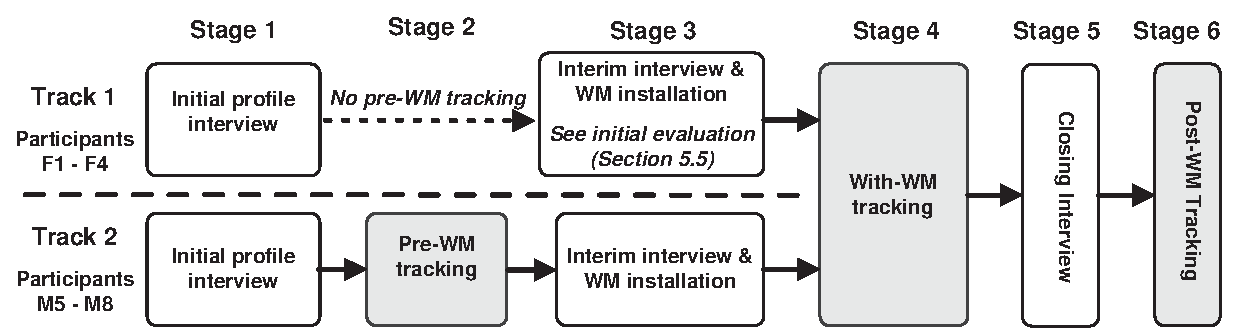
\includegraphics[width=\textwidth]{pictures/main-study/main-study-method.pdf}
	\end{center}
	\caption{Main Study: overview of method}
	\label{fig:main-study:method-overview}
\end{figure}

%%%%%%%%%%%%%%%%%%%%%%%%%%%%%%%%%%%%%
% MUST EXPLAIN TWO TRACKS CLEARLY
% Or consider merging!
%%%%%%%%%%%%%%%%%%%%%%%%%%%%%%%%%%%%%
% Eight participants took part in the study, during which WE tracked the evolution of the three collections and the strategies used to manage them. Participation was divided across two different tracks:
\textbf{Figure~\ref{fig:main-study:method-overview}} shows how the two tracks differed in terms of their participation in the various stages of the study.  In summary, the track 1 participants did not take part in stage 2 (pre-WM tracking), as stages 1 and 3 (the initial and interim interviews) were combined in the initial evaluation reported in \textbf{Chapter~\ref{chapter:design}}.  Therefore they proceeded straight on to stage 4.  \textbf{Table~\ref{table:main-study:participation}} provides a detailed breakdown of participation on an individual basis.

%%%%%%%%%%%%%%%%%%%%%%%%%%%%%%%%%%%%%%%%%
% Multiple methods of data collection
%%%%%%%%%%%%%%%%%%%%%%%%%%%%%%%%%%%%%%%%%
% to reduce inappropriate certainty, and enhance interpretability. 
% TODO: emphasise exploratory nature more?
% Report difficulty in diaries
Throughout the study, data was collected through a range of methods including interviews, diary and logging.  A range of methods were employed for two reasons.  Firstly, it was envisaged that their triangulation would help build a rich picture of participants' behaviour. 
%For instance, it was hoped that the log data would act as a reference during the interviews.
Secondly, the author also had an interest in exploring the worth of each method.
% triangulation
% The multiple data sources were triangulated as described in \textbf{Section~\ref{main-study:method:triangulation}}. 

The following sections discuss each stage of the study in more detail.
% Refer to experimental material in appendix (eg. q'aire). 
Copies of the experimental materials are included in \textbf{Appendix~\ref{chap:appendices-main-study-material}}. % \textit{NB: need to mention that F1--F4 had a different profiling questionnaire?}




%%%%%%%%%%%%%%%%%%%%%%%%
% STAGE 1: PROFILING
%%%%%%%%%%%%%%%%%%%%%%%%
%%%%%%%%%%%%%%%%%%%%%%%%%%%%%%%%
\subsubsection{Stage 1: Initial Interview (all participants)}
%%%%%%%%%%%%%%%%%%%%%%%%%%%%%%%%
% Much as per Chapter 4, avoid big repeat. 
% Need to repeat: Prelims (e.g. disclosure agreement)
% Need detail on interview structure: background expertise, general survey of computer usage, how organized do you consider yourself?, guided tour (practices, satisfaction, integration with other tools), todo items, change anything. Also asked about requirements for integration.
% Questionnaire design?  See appendix.
The initial interview followed a similar format to that employed in the exploratory study in \textbf{Chapter~\ref{chapter:exploratory_study}}\footnote{Profiling interviews were not carried out for participants F1 and F2 since they had already taken part in the exploratory study.}.  Participants were asked about their PIM practices regarding files, email and bookmarks in turn.   An additional question was added regarding views on existing levels of integration between the three PIM-tools.  Note that the privacy precautions outlined in \textbf{Chapter~\ref{chapter:exploratory_study}} were also followed here.
% Regarding WorkspaceMirror, not told (too much) about nature of tool in advance
Studies were carried out in the work environment of the participant and took about one hour.  All interviews were recorded on mini-disc and fully transcribed.

In the exploratory study, folder structures had been recorded via a screenshot and transcribed by hand.  To automate this process in the main study, a tool called \textit{WorkspaceSnapper} (WS) was developed by the author.  WS recorded the file, email and bookmark folder structures as a text file, along with counts of items within folders.  To limit intrusion, details of specific items -- such as filenames -- were not recorded.  During the interview, WS was installed and used to obtain snapshots of the initial folder structures.  Participants were shown the resulting text file to alleviate any privacy concerns. After the profiling interview,  WS was left installed.

%Analysis: organizational dimensions, cross-tool profiling as in \textbf{Chapter~\ref{chapter:exploratory_study}}.  
%Starting point for workspace evaluation transcript.
% Data analysis is described in \textbf{Section~\ref{main-study:method:triangulation}}




%%%%%%%%%%%%%%%%%%%%%%%%
% STAGE 2: PHASE 1
%%%%%%%%%%%%%%%%%%%%%%%%
%%%%%%%%%%%%%%%%%%%%%%%%%%%%%%%%%%%%%%%
\subsubsection{Stage 2: Pre-WM Tracking (track 2 participants only)}
%%%%%%%%%%%%%%%%%%%%%%%%%%%%%%%%%%%%%%%
% Refer to experimental material in appendix (eg. q'aire)
The PIM practices of the four \textit{track 2} participants (M5--M8) were observed over several weeks \textit{before} WM was installed\footnote{The track 1 participants were directly exposed to WM during the initial evaluation reported in \textbf{Chapter~\ref{chapter:design}}, and therefore did not take part in stage 2.}.  This was done to characterise their ``normal'' PIM behaviour, and so better ascertain the effect of the design intervention. Average participation in stage 2 was 57 days (min: 32, max: 75, SD: 21.6).  Multiple methods of data collection were employed to help build up a rich picture of participants' behaviour:

\begin{itemize}
%%%%%%%%%%%%%
% Snapshots
%%%%%%%%%%%%%
\item \textit{Snapshots of the three folder structures} -- Participants were asked to manually initiate snapshots using WorkspaceSnapper to lessen the infringement of their privacy.  Snapshots were requested via email at two-week intervals. % returned as zipped email

%%%%%%%%%%%
% DIARY
%%%%%%%%%%%
\item \textit{Diary} -- Participants were also asked to keep a diary of significant incidents relating to the management of the three collections. Two incidents were provided as examples: (1) creating a new folder, and (2) failing to locate an item.  % The diary template is shown in \textbf{Appendix~\ref{chap:appendices-main-study-material}}.

\end{itemize}


%%%%%%%%%%%%%%%%%%%%%%%%%%
% AVERAGE PARTICIPATION
%%%%%%%%%%%%%%%%%%%%%%%%%%














%%%%%%%%%%%%%%%%%%%%%%%%
% STAGE 3: DESIGN INTERVENTION
%%%%%%%%%%%%%%%%%%%%%%%%
%%%%%%%%%%%%%%%%%%%%%%%%%%%%%%%%%%%%%%%%%%%%%%%%%%%%%%%%%%%
\subsubsection{Stage 3: Interim Interview (all participants)}
%%%%%%%%%%%%%%%%%%%%%%%%%%%%%%%%%%%%%%%%%%%%%%%%%%%%%%%%%%
% Design as an intervention in the study process.  
% interim interview + installation
%%%%%%%%%%%%%%%%%%%%%%%%%%%%%%%%%%%%%%

The \textit{track 2} participants then took part in a 30 minute interim interview\footnote{For the \textit{track 1 participants}, this stage was reported in the initial evaluation in \textbf{Chapter~\ref{chapter:design}}.}. Firstly, they were questioned regarding major events in the three collections of personal information over stage 2.  A transcript of folder changes and diary events was used as a shared resource in the interview (see \textbf{Section~\ref{main-study:method:data-analysis}}).
% showed how to create and delete a folder
Then, WM was installed on their machines, folder-mirroring was demonstrated by the author, and the participants were asked for their first impressions.

% \textit{Consider moving to next section}.
It was difficult to find users with a set of PIM-tools that were fully compatible with WM, and many potential participants had to be ruled out. \textbf{Table~\ref{table:main-study:participants-problems}} summarizes the incompatibilities encountered for the final participants which limited the extent of mirroring. In each case, they were asked to consider whether they would have mirrored events, and if so, to perform mirroring manually.
% These were primarily due to two reasons: (1) the wide range of PIM-tools in use, and (2) the relative immaturity of the prototype.
Participant M5 stored his personal files on a UNIX-based network drive which was incompatible with the file-monitoring capabilities of WM.  % of the \texttt{dotNetWatcher} component of 
Participants M3 and M7 managed files in two areas of the file system, whilst WM was limited to monitoring one area.  M4 and M5 used MS Outlook Express to manage email, rather than MS Outlook as required by WM.  M5 switched to MS-Outlook before installing WM, as he reported planning to do for some time.
%%%%%%%%%%%%%%%%%%%%%%%%%%%
% Installation problems
%%%%%%%%%%%%%%%%%%%%%%%%%%%
% As mentioned above, installation problems were encountered  (see \textbf{Table~\ref{table:main-study:participants-problems}}). 

%%%%%%%%%%%%%%%%%%%%%%%%%%%%%%%%%%%%%%%%%
% TABLE OF INSTALLATION PROBLEMS
%%%%%%%%%%%%%%%%%%%%%%%%%%%%%%%%%%%%%%%%%
\begin{table}[hbtp]
\begin{center}
\begin{footnotesize}
\setlength{\extrarowheight}{2pt}
\begin{tabular}{|c|p{4cm}|p{5cm}|p{2.4cm}|}
% Table generated by Excel2LaTeX from sheet '3 Installation problems'
\hline
  {\bf Participant} & {\bf File-related problems} & {\bf Email-related problems} & {\bf Bookmark-related problems} \\
\hline
        F1 &          - &          - &          - \\
\hline
        F2 &          - &          - &          - \\
\hline
        F3 & Personal files split over two areas of the file system (Desktop and My Documents) &          - &          - \\
\hline
        F4 &          - & Use of MS-Outlook Express (incompatible with WM) &          - \\
\hline
        M5 & Use of  network drive (incompatible with WM) & Use of MS-Outlook Express (incompatible with WM). User agreed to switch to MS-Outlook. &          - \\
\hline
        M6 &          - &          - &          - \\
\hline
        M7 & Personal files split over two areas of the file system (My Documents and `D' drive) &          - &          - \\
\hline
        M8 &          - &          - &          - \\
\hline
\end{tabular}  
\end{footnotesize}
\caption{WM installation problems: incompatibilities with PIM-tools}
\label{table:main-study:participants-problems}
\end{center}
\end{table}
\normalsize








%%%%%%%%%%%%%%%%%%%%%%%%
% STAGE 4: PHASE 2
%%%%%%%%%%%%%%%%%%%%%%%%
%%%%%%%%%%%%%%%%%%%%%%%%%%%%%%%%%%%%%%%%%%%%%%%%%%%%
\subsubsection{Stage 4: With-WM Tracking (all participants)}
%%%%%%%%%%%%%%%%%%%%%%%%%%%%%%%%%%%%%%%%%%%%%%%%%%%

The next stage involved the tracking of participants' PIM practices with WM installed. Average usage of WM was 44 days (min: 16, max: 93, SD: 50.4, see \textbf{Table~\ref{table:main-study:participation}} for more detail).

%%%%%%%%%%%%%%%%%%%%%%%%%%%%%%%%%%%%%%%%%%%%%%%%%%%%%%%%%
% Data collection: diary and log/snapshots as before
%%%%%%%%%%%%%%%%%%%%%%%%%%%%%%%%%%%%%%%%%%%%%%%%%%%%%%%%%
% Refer to experimental material in appendix (eg. q'aire)
Both methods of data collection from stage 2 were employed: (1) bi-weekly snapshots of the three folder structures captured with WS, and (2) a diary of significant events.  Additionally, two other forms of data collection were used.  Firstly, occasional interviews were carried out to check WM was working satisfactorily, and to get feedback. Secondly, WM maintained a log of mirroring events.  % During data analysis, data was triangulated into the workspace evolution transcript (see \textbf{Section~\ref{main-study:method:triangulation}}).
Apart from the early version used in the feasibility study, WM was robust and did not crash.  By default, WM was started automatically at start-up, and most participants left it running continuously whilst their computer was switched on.  % The next section focuses on the feedback obtained regarding the design of WM, rather than implementation details.


% as in Stage 2

%%%%%%%%%%%%%%%%%%%%%%%%
% STAGE 5: CLOSING INTERVIEW
%%%%%%%%%%%%%%%%%%%%%%%%
%%%%%%%%%%%%%%%%%%%%%%%%%%%%%%%%%%%%%%%%%%%%%%%%%%%
\subsubsection{Stage 5: Closing Interview (all participants)}
%%%%%%%%%%%%%%%%%%%%%%%%%%%%%%%%%%%%%%%%%%%%%%%%%%%

In the closing interview, participants were asked for feedback on the WM prototype via a series of questions addressing impact on file, email and bookmark management in turn.  % Participants were able to comment on any aspect of the design.
Secondly, participants were asked about changes to their PIM strategies over the course of the study to date, and what factors had influenced those changes.  Finally, WM was uninstalled from their computer\footnote{Participant F2 requested to keep WM, and continued to use it for 80 days after the study had finished}.  % A full copy of the closing interview can be seen in \textbf{Appendix~\ref{chap:appendices-main-study-material}}. % textit{NB: need to mention that different participants had different forms of the questionnaire?}


% appendix


%%%%%%%%%%%%%%%%%%%%%%%%%%%%%%%%%%%%%
% Refer to materials in appendix?
%%%%%%%%%%%%%%%%%%%%%%%%%%%%%%%%%%%%%

%%%%%%%%%%%%%%%%%%%%%%%%
% STAGE 6: CLOSING INTERVIEW
%%%%%%%%%%%%%%%%%%%%%%%%
%%%%%%%%%%%%%%%%%%%%%%%%%%%%%%%%%%%%%%%%%%%%%%%%%%%
\subsubsection{Stage 6: Post-WM Tracking (all participants)}
%%%%%%%%%%%%%%%%%%%%%%%%%%%%%%%%%%%%%%%%%%%%%%%%%%%

Approximately six months after the closing interview, participants were requested for a final snapshot using WS, after which it was uninstalled.

%%%%%%%%%%%%%%%%%%%%%%%%%%%%%%
% TABLE OF PARTICIPATION
%%%%%%%%%%%%%%%%%%%%%%%%%%%%%%
%%%%%%%%%%%%%%%
% TO PLACE
%%%%%%%%%%%%%%%
% MOVE TO METHOD/RESULTS
% All eight participants in the field study reported in this chapter installed and used WM within their day-to-day workspace for an average of 69 days (range: 16 to 143). 
Average total participation was 286 days (min 218, max 309, SD: 32.2). Participation in the different stages of the study varied between participants and is summarized in \textbf{Table~\ref{table:main-study:participation}}.

% \textbf{Table~\ref{table:main-study:participation}} provides more detail on participation in the six stages.

% The following sections discuss each stage of the study in more detail.


%%%%%%%%%%%%%%%%%%%%%%%%%%%%%%%%%%%%%%%%%%%%%%%%%%%
% TABLE X: STUDY PARTICIPATION PER PARTICIPANT
%%%%%%%%%%%%%%%%%%%%%%%%%%%%%%%%%%%%%%%%%%%%%%%%%%%
% Also consider table in Bellotti et al 2003
% Participation in the various stages of the study varied between participants as described in \textbf{Table~\ref{table:main-study:participation}}.
\begin{sidewaystable}% [hbtp]
\begin{center}
\begin{footnotesize}
\setlength{\extrarowheight}{2pt}
% Table generated by Excel2LaTeX from sheet 'Participation'
\begin{tabular}{|c|p{2cm}|p{2cm}|p{2cm}|p{2cm}|p{2cm}|p{2cm}|p{2.5cm}|}
\hline
{\bf Participant} & {\bf Stage 1: Initial interview} & {\bf Stage 2: Pre-WM tracking (\# days)} & {\bf Stage 3: Interim interview and WM installation} & {\bf Stage 4: With-WM tracking (\# days)} & {\bf Stage 5: Closing interview} & {\bf Stage 6: Post-WM tracking} & {\bf Total participation (\# days) } \\
\hline
F1 (track 1) & \checked (see exploratory study, \textbf{Chapter~\ref{chapter:exploratory_study}}) &          - & \checked (see initial evaluation in \textbf{Chapter~\ref{chapter:design}}) &         57 &   \checked &   \checked &        260 \\
\hline
F2 (track 1) & \checked (see exploratory study, \textbf{Chapter~\ref{chapter:exploratory_study}}) &          - & \checked (see initial evaluation in \textbf{Chapter~\ref{chapter:design}}) &        120 &   \checked &   \checked &        309 \\
\hline
F3 (track 1) &   \checked &          - & \checked (see initial evaluation in \textbf{Chapter~\ref{chapter:design}}) &        143 &   \checked &   \checked &        309 \\
\hline
F4 (track 1) &   \checked &          - & \checked (see initial evaluation in \textbf{Chapter~\ref{chapter:design}}) &        111 &   \checked &   \checked &        305 \\
\hline
M5 (track 2) &   \checked &         32 &   \checked &         65 &   \checked &   \checked &        219 \\
\hline
M6 (track 2) &   \checked &         75 &   \checked &         18 &   \checked &   \checked &        302 \\
\hline
M7 (track 2) &   \checked &         75 &   \checked &         16 &   \checked &   \checked &        306 \\
\hline
M8 (track 2) &   \checked &         46 &   \checked &         20 &   \checked &   \checked &        281 \\
\hline
{\bf Average (\#days)} &          - &         57 &          - &      68.75 &          - &          - &        286 \\
\hline
\end{tabular}  
\end{footnotesize}
\caption{Summary of participation in each stage of the main study}
\label{table:main-study:participation}
\end{center}
\end{sidewaystable}
\normalsize

%%%%%%%%%%%%%%%%%%%%%%%%%%%%%%%%%%%%%%%%%%%%%%%%%%%%%%%%%%%%%%%%%%%%%%%%%%%%%%%%%%%%%%%%%%%%%%%%%%%%%%%%%%
%%%%%%%%%%%%%%%%%%%%%%%%%%%%%%%%%%%%%%%%%%%%%%%%%%%%%%%%%%%%%%%%%%%%%%%%%%%%%%%%%%%%%%%%%%%%%%%%%%%%%%%%%%
%%%%%%%%%%%%%%%%%%%%%%%%%%%%%%%%%%%%%%%%%%%%%%%%%%%%%%%%%%%%%%%%%%%%%%%%%%%%%%%%%%%%%%%%%%%%%%%%%%%%%%%%%%
%%%%%%%%%%%%%%%%%%%%%%%%%%%%%%%%%%%%%%%%%%%%%%%%%%%%%%%%%%%%%%%%%%%%%%%%%%%%%%%%%%%%%%%%%%%%%%%%%%%%%%%%%%

%%%%%%%%%%%%%%%%%%%%%%%%
% DATA ANALYSIS
%%%%%%%%%%%%%%%%%%%%%%%%
%%%%%%%%%%%%%%%%%%%%%%%%%%%%%%%%%%%%%%%%%%%%%%%%%%%
\subsection{Data Analysis}
\label{main-study:method:data-analysis}
%%%%%%%%%%%%%%%%%%%%%%%%%%%%%%%%%%%%%%%%%%%%%%%%%%%
% Include: Learning from lessons of previous studies?

% % Four of our colleagues have been using WorkspaceMirror in their primary desktop workspaces over four months, and are providing feedback via diaries and weekly interviews.  WE have also correlated this qualitative data with fortnightly logs of their evolving folder hierarchies to track their usage of any mirrored folders.  WE triangulated the data to build up a rich picture of the user's attitude to WorkspaceMirror, and investigate whether it influenced their PIM practices.  
% Mass of data collected via the range of methods. Data overload!
% Data includes interviews, logs, and diaries from both before and after installation of WM.
% The preceding section describes how data was collected via a range of techniques to build up a rich picture of participants' PIM practices.
% This section discusses how the different forms of study data were processed and collated.

%%%%%%%%%%%%%%%%%%%%%%%%%%%%%%%%%%%%%%%%%
% ADD: whatabout questionnaire data?
%%%%%%%%%%%%%%%%%%%%%%%%%%%%%%%%%%%%%%%%%

%%%%%%%%%%%%%%%%%%%%%%%%%%%%%%%%%%%%%%%%
% content analsysi of interview data
% Extraction of critical incidents, most frequent and important issues and problems
% Quote extraction to illustrate main themes.
% to give idea of PIM behaviour (pre and post design intervention, and also usage of WM tool). 
%%%%%%%%%%%%%%%%%%%%%%%%%%%%%%%%%%%%%%%% 
% Content analysis was performed through a process of affinity clustering (CLARIFY).  Key themes were extracted and used to produce a coding scheme.  This was then applied across all participants.  Particular attention was paid to issues relating to WM, and to longitudinal PIM issues.
% Need to report to where it is reported?
All interview and diary data was transcribed into one text file for each participant.  An initial coding scheme was developed relating to areas of key interest: (1) feedback on WM, and (2) comments relating to changes in strategy.  The coding scheme was iteratively applied to the data, and extended with additional interesting themes that came to light.  A sample of the qualitative data collected is shown in \textbf{Appendix~\ref{chap:appendices--study-data}} on page~\pageref{chap:appendices--study-data:main-study}.

%%%%%%%%%%%%%%%%%%%%%%%%%%%%%%%%%%%%%%%%%%%%%%
% Analysis of folder structure snapshots
% Repeat of analyses from exploratory study, including folder overlap?
%%%%%%%%%%%%%%%%%%%%%%%%%%%%%%%%%%%%%%%%%%%%%%
The folder snapshots recorded in stage 1 were analysed in terms of \textit{organizational dimensions}, and \textit{folder overlap}.  Participants' organizing strategies were also characterized, and a cross-tool profile produced.  Please see \textbf{Chapter~\ref{chapter:exploratory_study}} for detail on these three techniques.
% Each participant's cross-tool profile was also collated based on their three tool-specific organizing strategies (see \textbf{Table~\ref{table:main-study:participants}}).

%%%%%%%%%%%%%%%%%%%%%%%
% Compilation of Workspace Evolution Transcript WET
%%%%%%%%%%%%%%%%%%%%%%%
% Triangulation of longitudinal data -- within Workspace Evolution Transcript, the collation of data from multiple methods between different data sources (objective and subjective). 
% Focus on monitored areas, but where users files split between multiple areas, took those into account.
All longitudinal data was collated into a \textit{workspace evolution transcript} (WET) for each participant. The WET included the following pieces of information:
\begin{itemize}
% evolution of folder structures and number of items. 

\item \textit{Incremental changes to the folder structures} -- These were identified manually for each of the three PIM-tools. Changes in the overall number of folders and unfiled items were also calculated to ascertain the growth of the collections.

\item \textit{Folder-related events} -- Events such as folder creation were identified and annotated with any relevant diary or interview comments.

\item \textit{Other events} -- Events that may have had an impact on PIM behaviour were also included, e.g. holidays, starting or finishing a project, or technical problems.

% \item Interview feedback relating to particular time periods was also used to annotate the WET.

\end{itemize}

%%%%%%%%%%%%%%%%%%%%%%%%%%%%%%%%%%%%%%%%%%%%%%%%%%%%%
% Analsysi of folder-re;lated events from Stage 4
%%%%%%%%%%%%%%%%%%%%%%%%%%%%%%%%%%%%%%%%%%%%%%%%%%%%%

Folder-related events in stage 4 were coded as follows:
\begin{itemize}
\item \textit{Type of folder event} -- Did the event relate to a creation, deletion, or renaming?
\item \textit{Source and trajectory of event} -- What was the source PIM-tool for the event: files, email or bookmarks?  What destination PIM-tools was the event mirrored to? (see \textbf{Figure~\ref{fig:main-study:trajectory}}).
\item \textit{Folder details} -- including name, organizational dimension, and depth
\item \textit{Was the event mirrored?}  -- Was WM used to mirror the folder event?  If so, which PIM-tools was it mirrored to?
\item \textit{Were the mirrored folders subsequently used?}  -- This was based on a simple criterion: did the folder contain any items at the end of stage 4?
\end{itemize}

Events were also annotated with relevant comments from the diaries and interviews. This highlighted examples of \textit{mistaken mirrorings} (when the participant did not intend to mirror an event, but did so accidently), \textit{missed mirrorings} (when a participant did not mirror, but subsequently indicated that it would have been useful to do so), and \textit{manual mirrorings} (when mirroring was performed by the participant, e.g. due to an incompatibility between WM and a PIM-tool).

\textbf{Table~\ref{table:main-study:wet-example}} shows a portion of the WET for participant F2 from during stage 4.  Each line in the table corresponds to one folder creation event.  The table shows seven mirrorings of creation events, six of which relate to a particular project, ``BOD'' (project name changed).   Each event is emboldened and underlined in the column corresponding to the source PIM-tool.  Mirrored folders are underlined and italicised.  For example, the first event shows a \texttt{Meetings} sub-folder being created under the \texttt{BOD} folder in the file collection, and mirrored to email only.   The final column indicates whether newly created folders were put to use by the end of stage 4.

% \textbf{Section~\ref{main-study:results:overview}} moves on by providing an overview of the results.

%%%%%%%%%%%%%%%%%%%%%%%%%%%%%%%%%%%%%%
% %%%%%%%%%%%%%%%%%%%%%%%%%%%%%%%%%%%%
% FIGURE - TRAJECTORY
% %%%%%%%%%%%%%%%%%%%%%%%%%%%%%%%%%%%%
%%%%%%%%%%%%%%%%%%%%%%%%%%%%%%%%%%%%%%
\begin{figure}[t]
	\begin{center}
		\leavevmode
		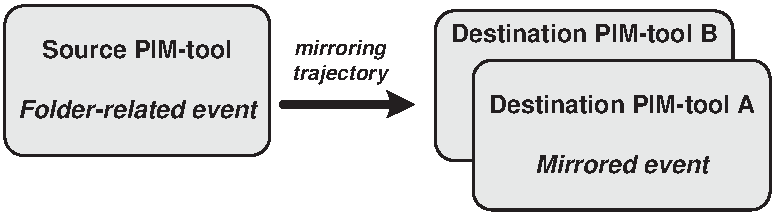
\includegraphics[height=2cm]{pictures/main-study/trajectory.pdf}
	\end{center}
	\caption{The trajectory of a mirroring event}
	\label{fig:main-study:trajectory}
\end{figure}

%%%%%%%%%%%%%%%%%%%%%%%%%%%%%%%%%%%%%%
% %%%%%%%%%%%%%%%%%%%%%%%%%%%%%%%%%%%%
% FIGURE - Sample from WET % Or a table?
% %%%%%%%%%%%%%%%%%%%%%%%%%%%%%%%%%%%%
%%%%%%%%%%%%%%%%%%%%%%%%%%%%%%%%%%%%%%
%%%%%%%%%%%%%%%%%%%%%%%%%%%%%%%%%%%%%%%%%
% TABLE OF PARTICIPANTS IN MAIN STUDY
%%%%%%%%%%%%%%%%%%%%%%%%%%%%%%%%%%%%%%%%%
\begin{table}[hbtp]
\begin{center}
\begin{footnotesize}
\setlength{\extrarowheight}{2pt}
% REMEMBER: replace _ WITH \_
% Table generated by Excel2LaTeX from sheet '5 WET sample'
\begin{tabular}{|c|p{2.5cm}|p{2cm}|p{2cm}|p{2cm}|p{2.5cm}|}
\hline
{\bf Date} & {\bf Folder event description (all are creation events)} & {\bf File system} & {\bf Email} & {\bf Bookmark} & {\bf Was folder used to store items by the end of stage 4?} \\
\hline
 12-Nov-02 & Mirror: from files to email & {\bf BOD/\underline{Meetings}} & {\it BOD/\underline{Meetings}} &    {\bf -} & Used in files (many subfolders), email (many subfolders) \\
\hline
 12-Nov-02 & Mirror: from files to email & {\bf BOD/Meetings/ \underline{TMT}} & {\it BOD/Meetings/ \underline{TMT}} &    {\bf -} & Used in files (2 subfolders), email (2 subfolders) \\
\hline
 12-Nov-02 & Mirror: from files to email & {\bf BOD/Meetings/ TMT/\underline{2002\_1113}} & {\it BOD/Meetings/ TMT/\underline{2002\_1113}} &    {\bf -} & Used in files (1 item), email (4 items) \\
\hline
 12-Nov-02 & Mirror: from files to email & {\bf BOD/Meetings/ \underline{PMC}} & {\it BOD/Meetings/ \underline{PMC}} &    {\bf -} & Used in email (1 subfolder) \\
\hline
 12-Nov-02 & Mirror: from files to email & {\bf BOD/\underline{papers}} & {\it BOD/\underline{papers}} &    {\bf -} & Used in files (6 items), email (1 item) \\
\hline
 21-Nov-02 & Not mirrored from files & {\bf BOD/WP4/ \underline{htmldocs}} &          - &    {\bf -} & Used in files (>10 items) \\
\hline
 28-Nov-02 & Mirror: from email to files and BM & {\it \underline{Context-Aware}} & {\bf \underline{Context-Aware}} & {\it \underline{Context-Aware}} & Used in files (12 items) \\
\hline
 02-Dec-02 & Mirror: from files to email & {\bf BOD/\underline{audit}} & {\it BOD/\underline{audit}} &          - & Used in files (9 items), email (12 items) \\
\hline
 02-Dec-02 & Not mirrored from files & {\bf BOD/WP4/ \underline{Mpeg7Schema}} &            - &          - & Used in files (>10 items) \\
\hline
 03-Dec-02 & Not mirrored from files & {\bf BOD/audit/ \underline{graf}} &          - &          - & Used in files (3 items) \\
\hline
 03-Dec-02 & Not mirrored from files & {\bf BOD/audit/ \underline{hutter}} &          - &          - & Used in files (3 items) \\
\hline
 04-Dec-02 & Mirror: from files to email and BM & {\bf BOD/WP4/ \underline{MPEGDocs}} & {\it BOD/WP4/ \underline{MPEGDocs}} & {\it BOD/\underline{WP4}/ \underline{MPEGDocs}} & Used in files (2 items), email (1 item) \\
\hline
 06-Dec-02 & Mirror: from email to files and BM & {\it BOD/\underline{FP6}} & {\bf BOD/\underline{FP6}} & {\it BOD/\underline{FP6}} & Used in files (3 items), email (13 items) \\
\hline
\end{tabular}  
\end{footnotesize}
\caption{Extract of the workspace evolution transcript from stage 4 for participant F2.}
\label{table:main-study:wet-example}
\end{center}
\end{table}
\normalsize



%%%%%%%%%%%%%%%%%%%%%%%%%%%%%%%%%
% FIN THESIS Chapter 6 MAIN STUDY METHOD
%%%%%%%%%%%%%%%%%%%%%%%%%%%%%%%%%

%%%%%%%%%%%%%%%%%%%%%%%%%%%%%%%%%%%%%%%%%%%%%%%%
% CHAPTER 6 -- MAIN STUDY
% RESULTS FROM WM EVAL
% File: tex/main-study-chapter/chapter6-main-study-RESULTS-WM.tex
%%%%%%%%%%%%%%%%%%%%%%%%%%%%%%%%%%%%%%%%%%%%%%%%%%%%%%%%%%%%%%%%%%%
%%%%%%%%%%%%%%%%%%%%%%%%%%%%%%%%%%%%%%%%%%%%%%%%%%%%%%%%%%%%%%%%%%%%%%%%%%%%%%%%%%%%%%%%%%
% Richard Boardman PhD Thesis: Improving Tool Support for Personal Information Management
%%%%%%%%%%%%%%%%%%%%%%%%%%%%%%%%%%%%%%%%%%%%%%%%%%%%%%%%%%%%%%%%%%%%%%%%%%%%%%%%%%%%%%%%%%
%%%%%%%%%%%%%%%%%%%%%%%%%%%%%%%%%%%%%%%%%%%%%%%%%%%%%%%%%%%%%%%%%%%%%%%%%%%%%%%%%%%%%%%%%%
% NATBIB NOTES
%%%%%%%%%%%%%%%%%%%
%\citet{jon90}                ->    Jones et al. (1990) 
%   \citet[chap.~2]{jon90}       ->    Jones et al. (1990, chap. 2)
%   \citep{jon90}                ->    (Jones et al., 1990) 
%   \citep[chap.~2]{jon90}       ->    (Jones et al., 1990, chap. 2) 
%%%%%%%%%%%%%%%%%%%%%%%%%%%%%%%%%%%%%%%%%%%%%%%%%%%%%%%%%%%%%%%%%%%%%%%%%%%%%%%%%%%%%%%%%%
%%%%%%%%%%%%%%%%%%%%%%%%%%%%%%%%%%%%%%%%%%%%%%%%%%%%%%%%%%%%%%%%%%%%%
% THINK
% Where are "`Other qualitative insights"' into PIM are reported.
% WHERE: lack of reflection with respect to PIM
%%%%%%%%%%%%%%%%%%%%%%%%%%%%%%%%%%%%%%%%%%%%%%%%%%%%%%%%%%%%%%%%%%%%%
%%%%%%%%%%%%%%%%%%%%%
% RESULTS ISSUES
%%%%%%%%%%%%%%%%%%%%%
% An illuminating set of results:
% THINK: some "study" results bridge the two Phases 1 and 2 (how to indicate?)
% how best to present results? - as case studies?}, , life events
% Highlight results that are new and those that merely confirm previous results, do they confirm/backup/agree/echo/support or contradict/clash/differ}
% THINK: note objective measures/subjective feedback below}
%	\item \textbf{A - Slice results by users}
%	%%%%%%%%%%%%%%%%%%%%%%%%%%%%%%%%%%%%%%%%%%%%
%	\begin{itemize}
%		\item A Cross-tool profiling of users - slice by user type
%		\item Extent of organization (as previous study)
%	\end{itemize}
%	\item \textbf{B - Slice results by information type/tool}
%	%%%%%%%%%%%%%%%%%%%%%%%%%%%%%%%%%%%%%%%%%%%%%%%%%%%%%%%%%%%%%
%	\begin{itemize}
%		\item Unimportance of bookmarks
%		\item Compare core objective stats - size, structure, growth etc.
%		\item User attitudes - Importance, control etc.
%		\item Comparing PIM practices in the three tools, strategies used in different aspects of PIM
%		\begin{itemize}
%			\item Organization: classication style/level of abstraction
%			\item Frequency of various activities
%		\end{itemize}
%		\item Comparing core characteristics of each information type table
%		\item Implications for unification - documents and stored email most similar (MOVE TO DISCUSSION?)
%	\end{itemize}
%	\item \textbf{D --PIM bugbears}
%	%%%%%%%%%%%%%%%%%%%%%%%%%%%%%%%%%
%		\item Break-down by tool/aspect of PIM
%		\item Long terms effects of problems
%		\item Severity increased by repetition?
%	\item \textbf{E -- Slice by production activity}
%	%%%%%%%%%%%%%%%%%%%%%%%%%%%%%%%%%%%%%%%%%%%%%%%%%%%


%%%%%%%%%%%%%%%%%%%%%%%%%%%%%%%%%%%%%%%%%%%%
%%%%%%%%%%%%%%%%%%%%%%%%%%%%%%%%%%%%%%%%%%%%
\newpage
\section{Overview of Results}
\label{main-study:results:overview}
%%%%%%%%%%%%%%%%%%%%%%%%%%%%%%%%%%%%%%%%%%%%
%%%%%%%%%%%%%%%%%%%%%%%%%%%%%%%%%%%%%%%%%%%%

%%%%%%%%%%%%%%%%%%%%%%%%%%%%%%%%%%%%%%%%%%%%%%%%%%
% Relate to process overview in figure above
%%%%%%%%%%%%%%%%%%%%%%%%%%%%%%%%%%%%%%%%%%%%%%%%%%
A sample of the qualitative data collected for each participant is shown in \textbf{Appendix~\ref{chap:appendices--study-data}} on page~\pageref{chap:appendices--study-data:main-study}. The results from the main study are divided into four sections as follows:
\begin{enumerate}

\item \textbf{Section~\ref{main-study:profiles}} provides a brief overview of participants' profiles.

\item Usage of WM varied dramatically between participants, along with their level of PIM activity. Therefore, \textbf{Section~\ref{main-study:case-studies}}, presents a case study summary of each participant. 

\item \textbf{Section~\ref{main-study:wm-analysis}} focuses on the evaluation component of the study.  Usage of WM is reported, along with participants' positive and negative feedback on the design.

\item Finally, \textbf{Section~\ref{main-study:longitudinal}} reports other findings, not directly related to the WM evaluation, such as changes in organizing strategy.
\end{enumerate}



%%%%%%%%%%%%%%%%%%%%%%%%
% Initial profiling
%%%%%%%%%%%%%%%%%%%%%%%%
%%%%%%%%%%%%%%%%%%%%%%%%%%%%%%%%%%%%%%%
\subsection{Participant Profiles}
\label{main-study:profiles}
%%%%%%%%%%%%%%%%%%%%%%%%%%%%%%%%%%%%%%%
% Probably don't need to go into massive detail here - just state when major difference from ES
% Effectively a repeat of exploratory study.  Cross-tool profiling etc.

%%%%%%%%%%%%%%%%%%%%%%%%%%%%%%%%
% Tool-specific strategies
%%%%%%%%%%%%%%%%%%%%%%%%%%%%%%%%
% The cross-tool profiling reported in  \textbf{Chapter~\ref{chapter:exploratory_study}} was carried out in an earlier stage in the study.

All eight participants actively collected files, email and bookmarks.  As in the exploratory study, behaviour varied between participants, and between tools for individual participants.  A brief summary is presented as follows.  All were active collectors and organizers of document files (average: 94 folders).  In email, seven participants had large inboxes. Three of these combined a large inbox with extensive filing (F1, F2 and F4).  Participant M6 pursued a frequent-filer strategy.  The remaining four participants, F3, M5, M7, M8, had large inboxes and filed only a few messages everyday.  On average, participants had  22 email folders.  Bookmarks were indicated to be of low importance by seven of the eight participants who collected them at a very low rate (average 15 folders).  There was one exception, participant F4, who collected bookmarks extensively, distorting the overall average total of bookmark folders up to 38.
%%%%%%%%%%%%%%%%%%%%%%%%%%
% Cross-tool profiles
%%%%%%%%%%%%%%%%%%%%%%%%%%
Cross-tool profiles were calculated using the method outlined in \textbf{Section~\ref{exp-study:Results-cross-tool-profiling}}: CT1 (3 participants), CT2 (2 participants), and CT3 (3 participants).  They are reported along with profile details in \textbf{Table~\ref{table:main-study:participants}}.
% Questionnaire responses to the extent to which they relied on folders in each tool supported the above.  Average responses were 5.3, 4.1, and 3.1 for files, email and bookmarks respectively.

%%%%%%%%%%%%%%%%%%
% Nature of work
%%%%%%%%%%%%%%%%%%
% ADD: nature of work (M6 as odd one out)
Seven of the eight participants were involved in long-term research, teaching, and administrative activities, reflecting their academic careers.  The one exception was participant M6.  He was as an undergraduate with a highly structured set of short-term activities corresponding to his degree courses . As in the exploratory study, all participants proved to be very open.  None of them restricted access to their personal collections.


%%%%%%%%%%%%%%%%%%%%%%%%%%%%%%%%%%
% Other profile discussion?
%%%%%%%%%%%%%%%%%%%%%%%%%%%%%%%%%%
% M6, M7 very confident -- different reason
% ADD: PIM level of confidence
% ADD: views on integration from questionnaire

%%%%%%%%%%%%%
% openness
%%%%%%%%%%%%%
% Compare with other researchers' experiences~\cite{Bellotti:00,Whittaker-email:96}
% Individual differences? (see below)












%%%%%%%%%%%%%%%%%%%%%%%%%%%%%%%%%%%%%%%%%%%%
%%%%%%%%%%%%%%%%%%%%%%%%%%%%%%%%%%%%%%%%%%%%
\newpage
\section{Participant Case Studies}
\label{main-study:case-studies}
%%%%%%%%%%%%%%%%%%%%%%%%%%%%%%%%%%%%%%%%%%%%
%%%%%%%%%%%%%%%%%%%%%%%%%%%%%%%%%%%%%%%%%%%%
% Need to mention installation issues?

As behaviour varied enormously between the eight participants, case study summaries of each are presented as follows. Each case study summarizes usage of WM, major events (e.g. OS reinstalls), and changes in PIM strategy.  % An ove

% The section is intended to provide a summary only, and more detail is provided in subsequent sections.  

% Changes in PIM strategy are discussed in more detail in \textbf{Section~\ref{main-study:longitudinal}}.

%%%%%%%%%%%%%%%%%%%%%%%%%%%%%%%%%%%%%%%%%%%%%%
% Discuss individual differences in depth?
%%%%%%%%%%%%%%%%%%%%%%%%%%%%%%%%%%%%%%%%%%%%%%
% variety of usage, "life events", core strategies (HL groups)
% Hard to generalize across users
% What I wanted: naturally occuring variations in use. Random events definitely prove that this was real



%%%%%%%%%%%%%%%%%%%%%%%
% Participant 6.1
%%%%%%%%%%%%%%%%%%%%%%%
\subsection*{Participant F1}
% No installation issues.
% Initially: positive
% cross-tool profile CT2 (F1, E2, B2)
% Ongoing incremental additions and structuring.
Participant F1, cross-tool profile CT2 (F1, E2, B2), was a male lecturer at Imperial College London (ICL).  Initially he was highly positive towards WM: \textit{``You only have to create a folder once ...  you create a [file] folder, you create a word document in that folder -- and the next thing you think oh I have to do a web search on the topic.  So you do a web search and you find some interesting websites, but you don't really have to think about where you're going to store those websites because you can put them in the folder that's already there''}.  However, although he ran WM for 57 days, he made relatively little use of it, only mirroring 4 folder creation events.  F1 explained that the low usage was due to the fact that he was changing university and had been away from his computer for long periods of time.  
% newly created folders between all three tools: 2 roles and 2 projects.
% (CHECK). Despite the relatively low use, 
After moving to his new job, he proceeded straight onto stage 6. However, in his closing interview he expressed a desire to continue using WM: \textit{``I would like to create equivalent folders in the file manager [to the `Eyegaze' email folder] but I haven't got time. I haven't got your program here''}.  In the process of moving, he transferred his files and email, but abandoned his bookmarks. This illustrates the relatively higher long-term value of those two collections.  





%%%%%%%%%%%%%%%%%%%%%%%
% Participant 6.2
%%%%%%%%%%%%%%%%%%%%%%%
\subsection*{Participant F2}
% No installation issues. 
% Participant 6.2 - ongoing incremental additions and structuring to all three collections.  
Participant F2, cross-tool profile CT1 (F1, E2, B1), was a male PhD student at ICL.  Out of all the participants, he made the most extensive use of WM -- mirroring 26 creation events over the 120 days he had WM installed.  Of these, 21 were related to a major group project called `BOD' (name changed).  His most common mirroring trajectory was files to email (18 events).   Of the 26 events, he identified 2 mistaken mirrorings, and 5 manual mirrorings (made when WM was not operating). He chose to carry on using WM after the closing interview for an additional 80 days.  His primary reason for using WM was to increase the consistency between different folder structures in support of his projects: \textit{``[WM] helps with project management. For example, I started the `BOD' project by creating a folder in email. Straight away, I was prompted whether I wanted it under documents as well. Therefore it was synchronized from the beginning rather than working in a hotchpotch''}.  He also stated that through the prompting, WM increased his reflection on PIM, resulting in an improved state of organization: \textit{``I think it's forced me to think about my workspace more, and in particular to synchronize between outlook and my files. Before I was not being methodical and I would lose track of things. Now things are more consolidated and structured''}.  Despite his take-up in mirroring, F2 did not make any significant changes in organizing strategy.  An extract from his WET is provided in \textbf{Table~\ref{table:main-study:wet-example}}.

%%%%%%%%%%%%%%%%%%
% OTHER QUOTES
%%%%%%%%%%%%%%%%%%
% Quite disorganized before - previously, I would create a one-off document folder, Now it helps me build a mental model of the mapping between different tools                                              % In an indirect way, forced me to think about why I was organizing my things the way I was doing. Trying to just manage project documents in DOCS/Project Documents area. Moved code elsewhere.            % May be more useful at the start of a new piece of work - or for people just starting out with a new computer, say new PhD students      
% Decisions of when/when not to mirror.
% Many design suggestions. 
% Examples of successful mirrorings, and ones used in the future.
% More folders in EM -> better



%%%%%%%%%%%%%%%%%%%%%%%
% Participant 6.3
%%%%%%%%%%%%%%%%%%%%%%%
\subsection*{Participant F3}
% very negative self-characterization
Participant F3, cross-tool profile CT3 (F1, E3, B2), was a male PhD student at ICL. He was highly organizing-neutral at the start of the study, \textit{``I'm lazy quite frankly. I don't naturally organize.  I'd have a pile as opposed to something filed.  And it's also partially due to the fact I have amazing spatial awareness really - I don't have to file things, I can remember [where they are]''}. Initially, he provided negative feedback with respect to WM, \textit{``Its just not my scene, you need someone else''}.

% Then, New Year reinvention
% Said study had greater influence than the tool
% Including move from My Docs (where WM is) to Desktop
However, 120 days into the study, he made a significant change in his file organizing strategy as part of a New Year resolution \textit{``to be more organized''}. In summary, he reorganized his files by moving his active documents to the desktop and creating a number of new folders there.  His change in strategy is discussed in detail in \textbf{Section~\ref{main-study:results:changes}}.
% Manual mirroring as dual file areas.
% Installation issues: dual docs (NO: after the move)
At that point he also started \textit{manually mirroring} new folders, between the Desktop and email (4 events).  He also used WM to mirror 5 folder creation events between ``My Documents'' and bookmarks.  Participant F3 thus provide a key example of emergent PIM behaviour which would not be clear from a one-off lab study. 

In the closing interview, he suggested that WM may be appropriate for someone setting up folder structures for the first time: \textit{``I'd say you get you'd get some seriously different results if you installed WM for someone with a brand new computer ... I think you'd get a very different dynamic, and you my might even get a completely different usage out of the same person. You installed it after `Downloaded Papers' was made in `My Documents'. If the mirror had opened up when I'd done that I would have said `yes stick it in the Favorites as well' ... but most of my pre-organization had already occurred by then, reasonably quickly after purchasing the computer''}.

% CHANGE, STUDY >> TOOL F3: F3: Do you know what ... the biggest... I don't know...  Overall the tool hasn't done that much, its more the conversations that me and you have. Its weird because I've become much more aware of all of my directory structures - there's a bit more thought trying to go into it and how its organized and stuff - but I think that's probably because of the conversations we have, i.e. being part of the user study than because of the tool.



%%%%%%%%%%%%%%%%%%%%%%%
% Participant 6.4
%%%%%%%%%%%%%%%%%%%%%%%
\subsection*{Participant F4}

% PROFILE
% Abandoned ``sub-collections'' of bookmarks.
Participant F4 was a female PhD student at ICL, with cross-tool profile CT1 (F2, E2, B1).  In stage 1, she complained in depth about not having enough time for PIM, and as a result feeling disorganized.  Despite this lack of time, she was the only participant to collect and structure bookmarks extensively. However, 70\% of her 250 bookmark folders had ``failed'' in terms of containing 2 items or fewer).  She had also restarted her bookmark collection three times, on each occasion storing the old collection in a ``\texttt{old Favourites 200x}'' sub-folder.

% WM installation
She provided positive initial feedback on WM, and made significant usage over the study -- mirroring 13 newly created folders, 8 of which were from bookmarks to files and email.  In particular, she welcomed the increase in consistency between folder structures: \textit{``Now its more consistent - and easier to remember. Good for tracking, makes it easier to remember where things are. It forces/reminds you to organize. When I've got a deadline, I save things anywhere. I plan to organize at a later date but never get round to it''}.
% F4: I did find it useful. Very useful. It does help me.
%F4: Good for keeping things consistent. Reminds me about parallel structures in email and file system   
%F4: It forces/reminds you to organize. When I've got a deadline, I save things anywhere. I plan to organize at a later date but never get round to it. Then maybe I have hassles later finding it... now the folder exists from somewhere else.
Due to the incompatibility of WM with her email client, MS-Outlook Express, she did not mirror to email, but reported that she would have found it useful to do so for many of the folders which related to conference submissions.
% , \textit{``I would mirror these [conference submissions] folders will involve email''}.
% Provide examples of missed mirroring?
In the closing interview, she also reported missing 2 potentially useful mirroring opportunities due to lack of time and dismissing the WM dialog box.

One limitation of WM that she identified was its focus on one area of the file system, and she requested WM support for mirroring between multiple file areas.  However, she also observed that the focus on one area had a key benefit: \textit{``It's good to have everything centralized into one directory. Before I had a problem remembering where to find things. Now it's more consistent - and easier to remember.  Previously I'd create a separate folder for each project or conference - but I'd put it anywhere. Mainly on my D-drive but it could be anywhere''}.





%%%%%%%%%%%%%%%%%%%%%%%
% Participant 6.5
%%%%%%%%%%%%%%%%%%%%%%%
\subsection*{Participant M5}
% large inbox, but frequent filer of some info
% QUOTE: irrationality of PIM
% Major reorganization of files and email 

Participant M5, cross-tool profile CT2 (F2, E2, B2), was a male PhD student at University College London (UCL).  He was one of two participants to make a change in organizing strategy, and cited the study participation as a key factor in reorganizing his files and email.  This change in strategy is discussed in detail in \textbf{Section~\ref{main-study:results:changes}}.
% CHANGE      
% [THIS IS MORE STUDY] M5: One definite effect: is that I have more folders in my email now. Before I had this huge inbox basically. So yeah - my email is definitely more structured as a result. It more or less introduced the concept of folders to my thinking about email organization.        
% SMALL CHANGE 
% M5: the folders that I've created, they only take up really minimal, you know - it might be smaller by 2% or 4% - and does that make a difference? Yes it does because most of the stuff that comes in is day-to-day stuff I deal with today or 2 days later - and the things I extract now are things with a longer due time.

% Two installation issues:
% email (changed) and network drive issues. Changed email tool.
% Network drive: major impact, inhibiting.
He encountered two installation issues with WM.  Firstly, his email tool was Outlook Express which  was incompatible with WM. However, as he had planned before the study, he switched to Outlook before installing WM. Secondly, he stored his personal files on a network drive which was incompatible with WM.  This had an impact on his usage of WM: ``\textit{The tool could not prompt me to mirror anything in Outlook because the only thing it could have prompted me for was the creation of bookmarks, which I don't use!  The ones that could have been useful it couldn't prompt me for because they were in the `H:' drive}''.  
% FILE: SPACE LIMITATION
% Ran out of space in document files - only user to remove stuff from document file collection.
%CHANGE Came round to WM at the end. Good quote to use.
%Another example of emergent behaviour
Also, he was initially negative towards WM, arguing that he made relatively little use of folders in email and bookmarks.
However, over the course of the study he \textit{manually} mirrored 4 folders between files and email, and was more positive by the closing interview: ``\textit{Quite impressively, the idea of mirroring structures in emails and in the folders didn't really cross my mind. I think before I had similarly named folders in both systems but they were never agreed in any way. And now I think the structures are a bit more coherent}''.  This represents a second example of emergent behaviour over time. % for why PIM-tools must be evaluated over the long-term. 

% PROMPTIONG UNANTICI
He also acknowledged the increase in reflection offered by WM:  \textit{``the act of being prompted ... is useful because it reminds you that you should think about how you should organize your stuff. But its also someone saying ``clean up your room''}. However, he interpreted this as a hint to do less PIM: \textit{``When I get the WM message up it reminds me that I'm wasting time with information management, creating folders and putting things in folders!''}.

% Participant M5 made a number of design suggestions included the need for more selective prompting, based on top-level folders only (see \textbf{Section~\ref{main-study:wm-analysis}}).
% PROMPTIONG ANNOYING
%M5: If prompting had worked - it might have increased my rating here but it might have also created my annoyance rating because I create folders so many times more in the file space,                 
%M5: Should not always prompt me, as I said before - it is not necessary to always replicate - it should prompt me in sensible cases. Maybe in higher-level folders, and not in lower level folders.                        



         







%%%%%%%%%%%%%%%%%%%%%%%
% Participant 6.6
\subsection*{Participant M6}
%%%%%%%%%%%%%%%%%%%%%%%

%%%%%%%%%%%%%
% profile
%%%%%%%%%%%%%
Participant M6, cross-tool profile CT1 (F1, E1, B1), was a male MSc. student at ICL.
% change
% No change over course of the study -- very settled. Archiving of email leads to net reduction in collection size. SETTLED.
% His PIM strategies did not change over the course of the study.
% wm
%Installation issues: none. Ideal pro-organizing profile (CT1) but highly negative of WM.
%Good quotes why.
He was initially negative towards WM.  % 
%%%%%%%%%%%%%%%%%%%%%
% bm-files partial
%%%%%%%%%%%%%%%%%%%%%
Although he was highly organized in all three tools, he considered his organizational needs to differ between them.  His files were extensively structured, but although he organized his email extensively, he only did so in a few top-level folders.  However, he observed a partial overlap between files and bookmarks: \textit{``Bookmarks and `My Documents' are very much more related to each other.  If you say in Bookmarks, \texttt{`my phd work'} and then underneath you have \texttt{`centra-fusion'} and \texttt{`cog-robotics'} and \texttt{research-labs} ... the first two you would have in files as well, but the third thing you probably wouldn't as you wouldn't put files in there''}. During the study, he only mirrored one folder creation, \texttt{Loreal}, from email to files, despite having no installation problems.

% he organized his email in a few top-level folders, whilst his files were organized in an extensive, deeply-nested folder structure.
%%%%%%%%%%%%%%%%%%%%%%%%%%%%%%%%%%%%%%%%%%%%%%%%%%%%%%%%%%%%%%%%
% Design suggestions. Email to files only (top-level only)
%%%%%%%%%%%%%%%%%%%%%%%%%%%%%%%%%%%%%%%%%%%%%%%%%%%%%%%%%%%%%%%%
% M6: So it does at the top-level maybe - yeah? The very top-level it does maybe, so if I have a folder phd maybe. Actually it goes one-way. If I create a folder in email there's likely to be a folder, a top-level folder in My Documents and in bookmarks relating to that which then may have sub-levels, or is very likely to have sublevels            
%F6: . Actually it goes one-way. If I create a folder in email there's likely to be a folder, a top-level folder in My Documents and in bookmarks relating to that
%F6 The very top-level it does maybe, so if I have a folder phd maybe. Actually it goes one-way. If I create a folder in email there's likely to be a folder, a top-level folder in My Documents and in bookmarks relating to that which then may have sub-levels, or is very likely to have sublevels.    
%F6: In my opinion it is "one to many", or like "one to a folder structure" really. You know ... its always email (one thing) links to one thing in my documents which does not necessarily have to be top-level, it could be above or could be in my documents directly but its just more likely to have another branches underneath.    
% So you know - they are more closely associated because you just don't do that many levels in email or I don't anyway.
At the end of the study, he suggested that mirroring should be one-way from email to files, for top-level folders only: \textit{``In my opinion it is `one to many', or like `one to a folder structure' really. You know ... its always email (one thing) links to one thing in my documents which does not necessarily have to be top-level, it could be above or could be in my documents directly but it's just more likely to have other branches underneath''}.  Again, this change in opinion regarding WM highlights the benefits of evaluating over the long-term.  M6 made no change in strategy over the course of the study.

% Speculation
% M6: highly-structured set of short-term activities in DOCS< little need to mirror across tools

% Prompts annoying
%M6: Because it kept on popping up and asking me the same silly question. I've had more annoying things - like my computer giving up ... WorkspaceMirror doesn't really irritate me. If I don't want it I just say cancel or just take the ticks out and click OK. Which I did at the beginning but then I realised I could just press cancel which was quicker. So you know I still am in control.Well its not really a problem since its just one cancel. Compared to what Word normally does to you, or Office or Windows - all kinds of harassing boxes - its negligible!  At least it never asked me to contact my system administrator!

%integ dangers
% M6: I would never give it to anyone who wasn't experienced at all ... because again it does a lot for you ... and most people, if they don't know what to do they just say "yes"! So if my mum was using it I would come home in the holidays and there would be 5000  folders, all empty, all her email lying in her inbox - you know what I mean ... You need someone who's at the stage of using a folder structure and understands folders and then yes.  
% F6: don't see the point of mixing the two except for confusing people like my mum, and then annoying me because I have to remind her that she's using the wrong piece of software. Anyone who knows how to use a computer won't use IE for organizing their files. The people who don't know enough get confused because they then don't see a difference between the internet and their own files (also see novice quote).

% flex
%M6: you might have to say "I don't want to create a folder, because that one already exists" ...
%
%Need for more mirroring flexibility/power #1: map to arb existing folders
%M6: Because you might start a project and not have an email folder but you receive so many emails on it that you create an email folder for it later ...
%
%Need for more mirroring flexibility/power #2: or map to new folders in any location
%M6: It would nice if you could browse and say "I want to create the folder at that level". You know a button "browse" where you can select where you want to create a new one. The default being "My Documents" because that'll be the case most of the time.



%%%%%%%%%%%%%%%%%%%%%%%
% Participant 6.7
\subsection*{Participant M7}
%%%%%%%%%%%%%%%%%%%%%%%

%%%%%%%%%%%%
% profile
%%%%%%%%%%%%
% ("ad hoc" organizer) - very settled. SETTLED
% separates created and downloaded
% org-neutral
Participant M7, cross-tool profile CT3 (F2, E3, B3), was a male PhD student at UCL.  He was \textit{organizing-neutral} in all three PIM-tools, and considered filing to be low priority.

% Initially negative - likes the principle but wants more power, But negative anyway
He responded unfavourably to WM from the start, expressing a requirement for a stronger form of integration between the tools: \textit{``My guess is I won't like it. I want something I can use in every tool. I want a tool with everything in it, so this isn't enough to warrant my adoption. I don't need it, as I don't organize with folders particularly. I mean I like the concept, the idea of unifying these working differences. I do think that's necessary and useful but I would want that next step - Version 2 or Version 10 - the complete new file-web and email manager - that would be interesting}''. He also foresaw that empty folders resulting from mirroring would cause a problem for him: \textit{``I'd like to create a folder that would be accessible from all three, rather than just an extra empty folder in the other two so I wouldn't get this massive bloat ... the problem with the mirroring is the empty folders ... and that to me would be annoying and would impact how I work}''.
% F7: Sharing I'd be a lot happier with, because it wouldn't impact at all the way I work currently ... so I'd create a folder but it would be accessible from all three - rather than just an extra empty folder in the other two.  So I wouldn't get this massive bloat ... the problem with the mirroring and the way I work is the lots of empty folders ... and that to me would be annoying and would impact how I work.
% M7: Well sharing means that the different objects (well files and email and bookmarks) actually share the same structure. Whereas mirroring means that the actual folder structure is copied but the actual contents of the folders in the bookmarks isn't visible from the email. For me mirroring is not really useful. Sharing I'd be a lot happier with, because it wouldn't impact at all the way I work currently ... so I'd create a folder but it would be accessible from all three - rather than just an extra empty folder in the other two.
% M7: Personally I don't see the need for mirroring ...I do see the need for sharing but mirroring ... because I don't organize things in a structure. I'm fairly haphazard ... if I want to put a folder there and not really bother .... but I don't specifically don't have to have it in my email management because  I don't have to cope with whatever I'm looking at on the web to be mirrored in my mail. For me mirroring is not really useful

% Therefore hard to evaluate.
% Multiple machines
%Logistical problems
%Also not used as little foldering. 
Despite not having any installation problems,  he made no use of WM during the trial: \textit{``There's been no chance - mainly because it hasn't actually done anything as I haven't actually created any folders. Also, even if I did, I haven't felt the need to mirror them''}. This illustrates the logistical challenge of evaluating PIM-tools via a field trial, the experimenter can not force the participant to use the designed functionality.

In the closing interview, although he had not used WM, he indicated that certain users may find it useful: \textit{``if they used the same kind of folder structures in the different applications ... I might recommend it because I'd see it as being useful for them conceptually to mirror the folder structures in the other environments}''.
% other users
% M7: I might do - especially if they used the same kind of folder structures in the different applications. If they did - I might recommend it because I'd see it as being useful for them conceptually to mirror the folder structures in the other environments. If there was someone who didn't use folders, or didn't work like that - I wouldn't bother.



%%%%%%%%%%%%%%%%%%%%%%%
% Participant 6.8
\subsection*{Participant M8}
%%%%%%%%%%%%%%%%%%%%%%%

Participant M8, cross-tool profile CT3 (F2, E3, B3), was a male research assistant at UCL.  He used the metaphor of a house to describe the different levels of organizing he employed in the three tools: ``\textit{my living room [file space] is really tidy because I've been making the effort to tidy it up. The rest of the house [emails and bookmarks] is a tip because everything I need is in the living room now ... Only certain elements are tidy. Other elements are rotting!}''

% wm
%Installation issues: none. Initially positive, but no usage -- although anticipated in different circumstances.
%Observes hurdle: major investment needed to rearrange document files. Bursty PIM quote
Although he encountered no installation problems with WM, and was initially positive, he made no use of it over stage 4. However, he remained positive about the tool: \textit{``Partially [I haven't used it] because I've been working on another machine.  And partially because I tend to have a structure which I put things in, keep that for a period of time, then have a spring-clean and change the structure. And I haven't been through the process of changing the structure with WorkspaceMirror running.  Its something that I'll do eventually, but I just haven't done my reorganization recently''}.
% M8: (DOCS/EM) well the use case here would be that there would be a document for a particular project or experiment or study in that case and I could just look at all my emails that relate just specifically to this project. I mean, its a different way of doing it to at the moment. At the moment I've got a HIGHERVIEW group that does contain anything about that project - so it would be a finer grain of categorization to organize my emails at that level which might be quite useful in terms of finding things again.
% M8: (DOCS/BM) Same reason for bookmarks - so again the documents are really the primary objects if you like, that need organizing, and then I'd have bookmarks relating to the studies that I was doing   - references, PDFs etc.
% M8: (EM/BM) For that I think of once case where I think it might: say for "web purchases" I might have a "shops" folder [in bookmarks] with links to shops that I've bought things from.
% M8: And it will homogenize that across my PDFs from the web, emails about a particular project, and files about a particular project. I could do that anyway without WorkspaceMirror but I don't ... Why not? Never really thought about it


Participant M8 made a number of design recommendations including the need to limit mirroring to top-level project folders: \textit{``once you've mirrored there [at the top-level] - you might not want to mirror it further down. I think it would work at that level. Here are the projects I'm working on.  Here are the emails about that project. And here are web links related to the project. That makes sense to me''}.

%One of the few participants to archive
%Archiving of email leads to net reduction in collection size. SETTLED



%%%%%%%%%%%%%%%%%%
%%%%%%%%%%%%%%%%%%
% ENDING
%%%%%%%%%%%%%%%%%%
%%%%%%%%%%%%%%%%%%
% Classify user behaviour, case studies to illustrate. 
% ADD Summary of section.
% Nominal clustering of participants based on their usage of WM?
% \textbf{Section~\ref{main-study:wm-analysis}} collates findings relating to the WM evaluation.




\newpage
%%%%%%%%%%%%%%%%%%%%%%%%%%%%%%%%%%%%%%%%%%%%%%
%%%%%%%%%%%%%%%%%%%%%%%%%%%%%%%%%%%%%%%%%%%%%%
\section{WM Evaluation}
% Alt titles:
% functional analysis a la Dumais et al 2001
% Qualitative analysis of results (but supported by objective data)
\label{main-study:wm-analysis}
%%%%%%%%%%%%%%%%%%%%%%%%%%%%%%%%%%%%%%%%%%%%%%
%%%%%%%%%%%%%%%%%%%%%%%%%%%%%%%%%%%%%%%%%%%%%%
%%%%%%%%%%%%%%%%%%%%%%%%%%%%%%%%%%%%%%%%%%%%%%
% THINK: anticipated/unanticipated results
% THINK: case studies
% THINK: relate to user types
%%%%%%%%%%%%%%%%%%%%%%%%%%%%%%%%%%%%%%%%%%%%%%

%%%%%%%%%%%%%%
% lead in
%%%%%%%%%%%%%%
The above case studies surveyed each participant's usage of WM in turn.  This section focuses in depth on the results from the WM evaluation.
%%%%%%%%%%%%%%%%%%%%%%%%%%%%%
% Structure of this section
%%%%%%%%%%%%%%%%%%%%%%%%%%%%%
% and also reports objective data from the With-WM tracking in stage 4. 
Firstly, \textbf{Section~\ref{main-study:results:themes-usage}} summarizes the usage of WM based on the objective data collected in stage 4. Then, \textbf{Section~\ref{main-study:results:themes-feedback}} presents qualitative feedback regarding WM, both positive and negative. Finally, \textbf{Section~\ref{main-study:results:themes-design-recs}} reports the design recommendations suggested by participants.
% Finally, \textbf{Section~\ref{main-study:results:themes-influences}} considers the factors which influenced the take-up of WM.


%%%%%%%%%%%%%%%%%%%%%%%%%%%%%%%%%%%
\subsection{Use of WM}
\label{main-study:results:themes-usage}
%%%%%%%%%%%%%%%%%%%%%%%%%%%%%%%%%%%
% MERGE WITH ABOVE
%%%%%%%%%%%%%%%%%
% Usage of WM
%%%%%%%%%%%%%%%%%
% Number of mirrors (as % of total events)
% Average depth
%%%%%%%%%%%%%%%%%%%%%%%%%%%%%%%%%%%%%%%%%%%%%%%%%%%%%%%%%%%%%%%%
% ADD: increased reliance on filing/folders at end of study?
% 6.2 - docs and email
% 6.4 documents
% M5 - email
%%%%%%%%%%%%%%%%%%%%%%%%%%%%%%%%%%%%%%%%%%%%%%%%%%%%%%%%%%%%%%%%%
% questionnaire responses - was it useful
% Impact on folder overlap?
% Types (orgdims) of mirrored folders
%%%%%%%%%%%%%%%%%%
% USAGE VARIED
%%%%%%%%%%%%%%%%%%

This section provides an overview of the objective data recorded during stage 4.
%%%%%%%%%%%%%%%%%%%%%%%%%%%%%%%%%%%%%%%%%%%%%%%%%%%
% SUMMARY - AVERAGE: DOES NOT REFLECT VARIATION
%%%%%%%%%%%%%%%%%%%%%%%%%%%%%%%%%%%%%%%%%%%%%%%%%%%
% % As noted above, usage of WM varied significantly between the participants (see \textbf{Table~\ref{table:main-study:wm-usage}} for a summary).  
% As indicated by the case studies, WM usage varied significantly between the participants.
In total, 57 \textit{folder creation events} were mirrored (not including test mirrorings performed during the interim interview).  However, the usage of WM varied widely between participants as indicated in the case studies above.  \textbf{Table~\ref{table:main-study:wm-usage}} provides an overview on an individual basis. 

%%%%%%%%%%%%%%%%%
% Usage of WM
%%%%%%%%%%%%%%%%%
% Other aspects to report:
% Number of mirrors (as % of total events)
% Average depth
% Creates versus deletes and renames + questionnaire responses
% Impact on folder overlap?
% Types (orgdims) of mirrored folders
Six of the 8 participants mirrored folder creation events during stage 4:
\begin{itemize}

\item Two participants, F2 and F4 made extensive use of WM, mirroring 26 and 13 newly created folders respectively, over an average of 116 days.  For F2, 21 folders related to his `BOD' project, and the most common source tool was files (20 folder creation events).  The most common organizational dimensions were \textit{project} (12) and \textit{event} (5).

For participant F4, the most common organizational dimensions for mirrored folders were \textit{project} (4), and \textit{event} (6).  The event-based folders related to conferences she was considering submitting papers to.  In contrast with F2, her most common source tool was bookmarks (10 folder creation events).

\item Participant F1, despite being very positive towards WM, only mirrored 4 folder creation events (all \textit{role} or \textit{project}).  He mirrored at least one event from each PIM-tool.  He highlighted his job change as a primary cause of his low PIM activity and WM usage.  

\item Participant M5 \textit{manually} mirrored 4 folders from files to email, with organizational dimensions \textit{project} (3), and \textit{document type} (1). He did not use WM to mirror due to its incompatibility with his Samba-based network drive.

\item After his New Year reorganization, Participant F3 \textit{manually} mirrored 4 folder creation events (3 from the `Desktop' to email, and 1 from `Desktop' to bookmarks).  He employed manual mirroring as WM was not compatible with the `Desktop' area of the file system.  He also used WM to mirror 5 events from files to bookmarks.  His events were based on a wide range of organizational dimensions including \textit{format} (2) and \textit{role} (2).

\item Participant M6 mirrored 1 \textit{project} folder from email to files. 

\end{itemize}

%%%%%%%%%%%%%%%%%%%%%%%%%%%%%%%%%%%%%%%%%
% TABLE: WM USAGE
% TO ADD: mirror events over which time span
% TO CHECK: mirrors/day
% EACH TIME I PASTE IN: CHECK %
% missed/manual/mistaken
% ++ days for F2
%%%%%%%%%%%%%%%%%%%%%%%%%%%%%%%%%%%%%%%%%
\begin{sidewaystable}
\begin{center}
\begin{footnotesize}
\setlength{\extrarowheight}{2pt} % 7 columns
% Table generated by Excel2LaTeX from sheet '4 Usage of WM'
\begin{tabular}{|c|p{1.3cm}|p{1.2cm}|p{1.2cm}|p{1.6cm}|p{2cm}|p{2cm}|p{1.8cm}|p{2.0cm}|p{1.4cm}|p{1.0cm}|p{1.0cm}|}
\hline
  {\bf ID} & {\bf Cross-tool profile} & {\bf Initial attitude to WM} & {\bf Final attitude to WM} & {\bf Installation problems, see also Table~\ref{table:main-study:participants-problems}} & {\bf Level of WM usage} & {\bf Source folder events in stage 4 (creates, deletes, renames)} & {\bf Folder creation events mirrored in stage 4} & {\bf Source tools and trajectories of mirrored events} & {\bf \% of folder creation events mirrored} & {\bf WM usage (\# days)} & {\bf Mirrors per day} \\
\hline
        F1 & CT2 (F1, E2, B2) &   Positive &   Positive &            & Some use before change of job & Files (3, 0, 0), Email (2, 0, 0), BM (0, 0, 0) &          4 & Source: files 2, email 2 & Files 66\%, EM 100\% &         57 &       0.07 \\
\hline
        F2 & CT1 (F1, E2, B1) &   Positive &   Positive &            & Extensive use, ongoing after study & Files (42, 3, 1), Email (7, 2, 0), BM (4, 0, 1) & 26 (5 manual, 2 mistaken) & Source: files 20, email 5, BM 1. Most common traj: ``files to email'' (18) & Files 48\%, EM 71\%, BM 25\% &        120 &       0.22 \\
\hline
        F3 & CT3 (F1, E3, B2) &   Negative &    Neutral &      files & Some use of WM. Started manual mirroring towards end of stage 4 & Files (71, 0, 20), Email (1, 0, 0), BM (1, 0, 2) & 9 (4 manual, 1 mistaken) & Source: files. ``Files to BM'' (5). ``Desktop to BM'' (4) & Files 13\%, EM 0\%, BM 0\% &        143 &       0.06 \\
\hline
        F4 & CT1 (F2, E2, B1) &   Positive &   Positive &      email & Extensive use & Files (23, 0, 0), Email (0, 0, 0), BM (14, 0, 0) &         13 & Source: files 2, BM 11. Most common traj: ``BM to files and email'' (8) & Files 9\%,  BM 79\% &        111 &       0.12 \\
\hline
        M5 & CT2 (F2, E2, B2) &    Neutral &   Positive & files, email & Some mirroring towards end of stage 4 & Files (14, 1, 7), Email (5, 3, 12), BM (0, 0, 0) & 4 (all manual) & Source: from files, to email only & Files 29\%, EM 0\% &         65 &       0.06 \\
\hline
        M6 & CT1 (F1, E1, B1) &   Negative &    Neutral &            &        Low & Files (12, 0, 0), Email (1, 0, 0), BM (0, 0, 0) &          1 & Source: from email, to files only. & Files 0\%, EM 100\% &         18 &       0.06 \\
\hline
        M7 & CT3 (F2, E3, B3) &   Negative &   Negative &      files &       None & Files (0, 0, 0), Email (0, 0, 0), BM (0, 0, 0) &          0 &          - &          - &         16 &       0.00 \\
\hline
        M8 & CT3 (F2, E3, B3) &   Positive &   Positive &            &       None & Files (4, 0, 0), Email (0, 0, 0), BM (0, 0, 0) &          0 &          - & Files 0\% &         20 &       0.00 \\
\hline
{\bf Total} &            &            &            &            &            &            &         57 &            &            &        550 &            \\
\hline
{\bf Average} &          - &          - &          - &          - &          - &            &          7 &          - &            &      68.75 &       0.07 \\
\hline
\end{tabular}  
\end{footnotesize}
\caption{Summary of WM usage}
\label{table:main-study:wm-usage}
\end{center}
\end{sidewaystable}
\normalsize

%%%%%%%%%%%%%%%%%%%%%%%%%%%%%%%%%%%%%
% Creates versus deletes and renames
%%%%%%%%%%%%%%%%%%%%%%%%%%%%%%%%%%%%%
% During stage 4, participants mirrored an average of 8 folder creations.  
One immediate observation is that all mirrored events related to \textit{folder creations}.  No participants used WM to mirror a folder delete or folder rename event, except to test the WM functionality during stage 3.  As reported in \textbf{Chapter~\ref{chapter:design}}, WM was limited to mirroring renaming events within a particular folder.  Renames corresponding to moving a folder between parent folders were not supported by WM, and resulted in a warning message being displayed.  However, no users reported encountering this over the study.
% However, M3 mirrored 2 folder deletes and 4 folder renames \textit{manually}.
Possible reasons for the bias in favour of creations over deletes and renames are discussed in \textbf{Section~\ref{main-study:discussion:evaluation}}. The rest of this section focuses on the mirroring of folder creation events.


%%%%%%%%%%%%%%%%%%%%%
% DEPTH and ORG DIM
%%%%%%%%%%%%%%%%%%%%%
Mirrored folders were high up in most participants' folder structures.  The average depth across all participants was 1.83 (SD: 0.89)\footnote{This was biased in favour of participant F2 who mirrored a number of deeper folders related to his `BOD' project. Without participant F2, the average depth was 1.43 (SD: 0.57).}.  A wide range of organizational dimensions were encountered.  Across all participants, the most common dimensions for mirrored folders were \textit{project} (40\%) and \textit{event} (22\%).  These aggregate figures are biased towards those participants who mirrored more folders (F2 and F4).

%%%%%%%%%%%%%%%%%%%%%%%%%%%%%%%%%%%%%%%%%%%%%%%%%
% TRAJECTORY
% Need to define source and destination tools?
% Mixture of trajectories.
% Source/destination tools F2 (D-E), F1 (DEB), F3 (DB), F4 (BD)
%%%%%%%%%%%%%%%%%%%%%%%%%%%%%%%%%%%%%%%%%%%%%%%%%
% F2 mirrored mostly from files to email, stating that he rarely used bookmarks so it was not worth mirroring to there.   F3 and F4 mirrored between files and bookmarks.  Note that possible trajectories were limited by encountered incompatibilities between WM and participants' PIM-tools.  Participant F4 was unable to mirror to email due to the incompatibility of Outlook Express. In contrast, the 4 events mirrored by participant F1 were based on creation events in all three PIM-tools.  The feedback presented in the next section shows a wide range of opinions from participants in terms of the form mirroring should take.
As noted above, participants employed WM with a range of mirroring trajectories.  \textbf{Table~\ref{table:main-study:trajectories}} summarizes the mirroring trajectories that were observed.  Across all participants, the most common source was files (64\% of all events), followed by bookmarks (21\%), and email (14\%).  The most common trajectories were \textit{``files to email''} (45\% of all events), \textit{``bookmarks to files and email''} (16\% of all events), and \textit{``files to bookmarks''} (13\% of all events). 

%%%%%%%%%%%%%%%%%%%%%%%%%%%%%%%%%%%%%%
% %%%%%%%%%%%%%%%%%%%%%%%%%%%%%%%%%%%%
% FIGURE - Sample from WET % Or a table?
% %%%%%%%%%%%%%%%%%%%%%%%%%%%%%%%%%%%%
%%%%%%%%%%%%%%%%%%%%%%%%%%%%%%%%%%%%%%
%%%%%%%%%%%%%%%%%%%%%%%%%%%%%%%%%%%%%%%%%
% TABLE OF PARTICIPANTS IN MAIN STUDY
%%%%%%%%%%%%%%%%%%%%%%%%%%%%%%%%%%%%%%%%%
\begin{table}[hbtp]
\begin{center}
\begin{footnotesize}
\setlength{\extrarowheight}{2pt}
\begin{tabular}{|p{1.1cm}|p{1.4cm}|p{1.5cm}|p{1.5cm}|p{1.5cm}|p{1.5cm}|p{1.5cm}|p{1.5cm}|}
\hline
{\bf Source PIM-tool} & {\bf \# mirrored creation events} & {\bf Destination: files} & {\bf Destination: email } & {\bf Destination: BM} & {\bf Destination: files and email} & {\bf Destination: files and BM} & {\bf Destination: email and BM} \\
\hline
{\bf Files} &         36 &          - &         25 &          7 &          - &          - &          4 \\
\hline
{\bf Email} &          8 &          3 &          - &          0 &          - &          5 &          - \\
\hline
  {\bf BM} &         12 &          2 &          1 &          - &          9 &          - &          - \\
\hline
\end{tabular}  
\end{footnotesize}
\caption{Trajectories of mirrored folder creation events (all participants)}
\label{table:main-study:trajectories}
\end{center}
\end{table}
\normalsize

% PERCENTAGE OF FOLDER EVENTS MIRRORED  \textbf{Section~\ref{main-study:results:growth}} reports the growth of the three collections over the length of the study.  
% For these five participants, the percentages of folder creation events mirrored was as follows. XX\% of file folder creations were mirrored.  The rates for email and bookmark folder creation events were YY\% and ZZ\% respectively.
% PERCENTAGE OF FOLDER EVENTS MIRRORED  \textbf{Section~\ref{main-study:results:growth}} reports the growth of the three collections over the length of the study.  
For the six participants who used WM, the percentage of total folder creation events that were mirrored varied substantially.  For example, participant F2 mirrored the most folder creation events, 26. Twenty were in files (equivalent to 48\% of all file-based creation events), 5 were in email (71\% of email creation events), and 1 was in bookmarks (25\% of BM creation events). \textbf{Table~\ref{table:main-study:wm-usage}} provides a detailed summary for each participant.% In contrast, participant M6 chose to not mirror any of the 12 file folders he created during stage 4. The one email folder that he mirrored was the only one he created.

%%%%%%%%%%%%%%%%%%%%%%%%%%%%%%
% PEOPLE WHO DIDN'T MIRROR
%%%%%%%%%%%%%%%%%%%%%%%%%%%%%%
The remaining two participants, M7 and M8, made no use of WM.  However, they both ran WM on their computers to test its robustness, and provided qualitative feedback.
%%%%%%%%%%%%%%%%%%%%%%%%%%%%%%%%%%%%%%%%%%%
% Difference between track 1 and track 2
%%%%%%%%%%%%%%%%%%%%%%%%%%%%%%%%%%%%%%%%%%%
% The difference is marked between the participants from \textit{track 1}, compared to those from the second track.
% Track 1 used WM for longer but NB: bugs and interrupted.
Overall, there was a marked difference between the track 1 and track 2 participants, who mirrored an average of 14 folders, and 1.5 folders respectively.  Possible reasons for this variation are discussed in \textbf{Section~\ref{main-study:discussion:evaluation}}.
% However, two of them (M6 and M8) found some aspects of the idea attractive.  % 
% The other four experimented with WM but did not use it in the long-term.  
% Possible reasons for this are discussed in \textbf{Section~\ref{main-study:wm-analysis}}.






















%%%%%%%%%%%%%%%%%%%%%%%%%%%%%%%%%%%
\subsection{Feedback from WM Users}
\label{main-study:results:themes-feedback}
%%%%%%%%%%%%%%%%%%%%%%%%%%%%%%%%%%%

%This section reports the benefits reported from those participants who employed WM., extracts common themes from the case studies, 

%%%%%%%%%%%%%%%%%%%%%%%%%%%%%%%%%%%%%%%%%%%%%
\subsubsection{Pros and Cons of Mirroring}
%%%%%%%%%%%%%%%%%%%%%%%%%%%%%%%%%%%%%%%%%%%%%

% Quotes from F1, F2 and F4. Even F3, F5, change.
% Others did not use it but acknowledged potential benefits (M8)
The core aim of the WM evaluation was to investigate whether the participants would use it to share folder structures between the PIM-tools.  A range of positive and negative feedback was received regarding the current design of WM.

The two heaviest users, F2 and F4, both observed and welcomed the increase in consistency, and described how it helped them manage information for a variety of projects (see case studies above). Both also suggested that mirroring lead to easier navigation, e.g. F2: \textit{``Its easier to navigate with a mirrored structure, compared to three different ones''}.  
%%%%%%%%%%%%%%%%%%%%%%%
% USERS WHO SWITCHED
%%%%%%%%%%%%%%%%%%%%%%%
Three participants (F1, F3, and M5) who performed more limited mirroring also acknowledged the benefits of an increase in consistency.  In addition, participant M8 who did not use WM, imagined that its use would offer benefits: ``\textit{It will homogenize that across my PDFs from the web, emails about a particular project, and files about a particular project. I could do that anyway without WorkspaceMirror but I don't ... Why not? Never really thought about it. The use case here would be that there would be a document for a particular project or experiment or study in that case and I could just look at all my emails that relate just specifically to this project. I mean, it's a different way of doing it to at the moment. At the moment I've got a `ProjectX' group that does not contain anything about that project.  So it would be a finer grain of categorization to organize my emails at that level which might be quite useful in terms of finding things again}''.
% M8: (DOCS/BM) Same reason for bookmarks - so again the documents are really the primary objects if you like, that need organizing, and then I'd have bookmarks relating to the studies that I was doing   - references, PDFs etc.
% M8: (EM/BM) For that I think of once case where I think it might: say for "web purchases" I might have a "shops" folder [in bookmarks] with links to shops that I've bought things from.


%%%%%%%%%%%%%%%%%%%%%%%%%%%%%
% BETWEEN WHICH TOOL
%%%%%%%%%%%%%%%%%%%%%%%%%%%%%
% FILES AND EMAIL								F5 F6 F7 F8
% FILES AND EMAIL AND BOOKMARKS	F1 F2 F3 F4 
In the closing study, 4 participants (F1, F2, F3, F4) indicated that mirroring was useful between all three tools, whilst 4 (F5, F6, F7, F8) indicated that it was most worthwhile between files and emails.  Note that all members of this second group placed little importance on mirroring to their bookmark collections.

%%%%%%%%%%%%%%%%%%%%%%%%%%%%%%%%%%%%%%%%%%
% THINK: benefits in different tools
% INCLUDE? Particular bonus in email.
%%%%%%%%%%%%%%%%%%%%%%%%%%%%%%%%%%%%%%%%%%
% \item  Tentative evidence of leveraging file investment across other tools? (F2)

%%%%%%%%%%%%%%%%%%%%%%%%%%%%%%%%%%%%%%%%%%%%%%%%%%
% However feedback: not 1:1 mapping (see below)
%%%%%%%%%%%%%%%%%%%%%%%%%%%%%%%%%%%%%%%%%%%%%%%%%%%
% However, all eight participants noted that there was not necessarily a one-to-one mapping between the folder structures in the different tools.  This is discussed below.
% In some cases a certain tool requires greater organizational granularity than another tool for a particular cross-tool activity.  
However, a general theme mentioned by all eight participants was that mirroring should not follow a one-to-one mapping between PIM-tools due to differing organizational requirements.  In many cases, participants had more complex organizing requirements in their file collections compared to email and bookmarks, e.g. F5: ``\textit{It doesn't make sense to create an email folder for every single publication so I just have a single submissions folder that goes across the publications and has, let's say,  at the moment maybe 30 entries or so. In my H-drive on the other hand, every single publication is a project  - and deserves its own folder because it consists of much more files than just the five emails. So that's an example where it makes sense that H-drive and email correspond but are not exactly mirrored}''.  

%%%%%%%%%%%%
% CLUTTER
%%%%%%%%%%%%
M7 felt that mirroring would result in clutter due to unused empty folders.  However, comments from several other participants suggested that they felt the benefits of increased consistency between folder structures outweighed the risk of clutter.  For example, F3 welcomed having folders mirrored and ready for use in the future, even if they were not used immediately, \textit{``I haven't written any latex so I haven't used it, but I'm keeping it.  I think it may be useful''}.  

%%%%%%%%%%%%%%%%%%%%%%%%%%%%%
% Top-level folders only
% Less power e.g. high-level categories most effective to share
% backed up by objective data? (F1, F2, F3, F4, M5, M6, M8)
%%%%%%%%%%%%%%%%%%%%%%%%%%%%%
Seven participants suggested that mirroring was particularly appropriate for \textit{top-level folders}, e.g. M8: \textit{``Images related to my project and all the substructure of that project ... it's very difficult to see why you'd want to mirror all that.  Once you've mirrored there [at the top-level] - you might not want to mirror it further down. I think it would work at that level. Here are the projects I'm working on.  Here are the emails about that project. And here are web links related to the project. That makes sense to me''}.
% M7: First impression good but not clear that it mirrored the whole structure
% Probably wouldn'tt mirror stuff that deep: experiments/study ....
% M6
% QUOTE:F3: Need for top-level only
% In a way My Documents - I could have a top-level one called Alfebitte which branched into presentations, deliverables, you know book chapters, experimental results, programming code - I could do that and that would have then mirrored to email... and probably bookmarks as well. But because... in a way because there was already a folder hierarchy partly made before I started using the FolderMirror... that might you know... yeah, because I just created the experiment results folder but if I'd been creating just an Alfebitte folder I would have mirrored it in all three. But specifically the one with results, there was no need to mirror it. But the top-level idea of the whole project, yes - I would have mirrored.
%%%%%%%%%%%%%%%%%%%%%%%%%%%%%%%%%%%%%%%%%%
% Partial mirroring (different schemas)
%%%%%%%%%%%%%%%%%%%%%%%%%%%%%%%%%%%%%%%%%%
% \item \textit{Selective mirroring} -- A variation to the core desktop functionality would be to mirror only parts of the folder hierarchies between tools (for example, two participants in the initial evaluation stated that mirroring was most appropriate for top-level folders).

\textbf{Section~\ref{main-study:results:themes-design-recs}} reports design suggestions relating to making mirroring more selective.

%%%%%%%%%%%%%%%%%%%%%%%%%%%%%
\subsubsection{Prompting}
%%%%%%%%%%%%%%%%%%%%%%%%%%%%%
%%%%%%%%%%%%%%%
% Prompting (both positive and negative wrt current design) (F3, F4, M6)
%%%%%%%%%%%%%%%
% The participants had a range of views on the existing prompting functionality.  Several found it annoying, and suggested possible alternatives.  \textit{Overhead of prompting.  Participant F4 clicking OK and closing box, and just mirroring to get it out of the way.  In other words, extra overhead is being created.}
% Prompts annoying
% ... WorkspaceMirror doesn't really irritate me. If I don't want it I just say cancel or just take the ticks out and click OK. Which I did at the beginning but then I realised I could just press cancel which was quicker. So you know I still am in control.Well its not really a problem since its just one cancel. Compared to what Word normally does to you, or Office or Windows - all kinds of harassing boxes - its negligible!  At least it never asked me to contact my system administrator!
% M7: I'd create a folder but it would be accessible from all three - rather than just an extra empty folder in the other two.  So I wouldn't get this massive bloat ... the problem with the mirroring and the way I work is the lots of empty folders ... and that to me would be annoying and would impact how I work.
% DESIGN: M6: Another thing there is that I had another folder in my email under phd, and I created a subfolder of that - then it would realise that phd was associated with that in files and then would create the folder beneath it.% Prompting (both positive and negative wrt current design) (F3, F4, M6)
%%%%%%%%%%%%%%%
%%%%%%%%%%%%%%%%%%%%%%%%%%%%%%%%%%%%%%%%%%%%%%%%%%%%
% Dislike of prompting by M7. (see design issues)
%%%%%%%%%%%%%%%%%%%%%%%%%%%%%%%%%%%%%%%%%%%%%%%%%%%%
% In addition, both M6 and M7 disliked prompting as they found it disruptive. M6: \textit{``Because . I've had more annoying things ... like my computer giving up!''}.
Participants had a range of views on the prompts generated by WM.  Three (M5, M6, M7) found it annoying, and suggested possible alternatives.  For example, M5 suggested WM should prompt more selectively: \textit{``It is not necessary to always replicate - it should prompt me in sensible cases. Maybe in higher-level folders, and not in lower level folders''}.  However, M6 noted that it was only a minor problem, \textit{``It kept on popping up and asking me the same silly question ... Well it's not really a problem since its just one cancel. Compared to what Word normally does to you, or Office or Windows - all kinds of harassing boxes - its negligible''}.

% \textit{Overhead of prompting.  Participant F4 clicking OK and closing box, and just mirroring to get it out of the way.  In other words, extra overhead is being created.} 
Three participants (F2, F3, F4) highlighted the extra decision-making introduced by WM -- i.e. deciding whether to mirror a folder event between tools.  This contributed to a number of missed and mistaken mirrorings:

%%%%%%%%%%%%%%%%%%%%%%%%%%%%%%%%%%%%%%%%%%%%%%%%%%%%%%%%%
% \subsubsection{Manual, missed and mistaken mirrorings}
%%%%%%%%%%%%%%%%%%%%%%%%%%%%%%%%%%%%%%%%%%%%%%%%%%%%%%%%%

\begin{itemize}
%%%%%%%%%%%%%%%%%%%%
% missed mirrors
% \item Missed (F3, F4)
%%%%%%%%%%%%%%%%%%%5

\item Both F3 and F4 reported missing 2 useful mirroring opportunities since they did not always have time for making such a decision and just pressed the `cancel' button on the WM dialog, W4: \textit{``It would have been useful to mirror to email but I didn't as there was no time, it [the associated work] was a deliverable''}.  
% F3:  \textit{``I might have just clicked automatically `no' without really thinking about it''}.  

%%%%%%%%%%%%%%%%%%%%%%%
% MISTAKEN MIRRORINGS
%%%%%%%%%%%%%%%%%%%%%%%
\item There were also a number of \textit{mistaken mirrorings} reported by participants F2 and F3 (2 and 1 respectively).  Again, participant F3 highlighted rushed mirroring decisions to be the key cause, in which he just clicked the `OK' button on the WM dialog box.

\end{itemize}

% Not all mirrorings were ``plain vanilla''. 
%%%%%%%%%%%%%%%%%%%%%%%%%%%%%%%%%%%%%%%%%
% MANUAL mirrors -- move to qualitative?
% \item Manual (F2, F3)
%%%%%%%%%%%%%%%%%%%%%%%%%%%%%%%%%%%%%%%%%
Three participants (F2, F3, and M5) reported carrying out \textit{manual mirroring}.  F2 did so when WM was not running.  The other two performed manual mirroring due to WM incompatibilities (see \textbf{Table~\ref{table:main-study:participants-problems}}). F3 manually mirrored 4 folders from the `Desktop' to his bookmarks, and M5 manually mirrored 2 folders from his network drive to email.


%%%%%%%%%%%%%%%%%%%%%%%%%%%%%%%%%%%%%%%%
\subsubsection{Getting Started with WM}
%%%%%%%%%%%%%%%%%%%%%%%%%%%%%%%%%%%%%%%%

%%%%%%%%%%%%%%%%%%%%%%%%%%%%%%%%%%%%%%%%%%%%%%%%%
% Difficulty of use when setting up (F3 and M8). 
%%%%%%%%%%%%%%%%%%%%%%%%%%%%%%%%%%%%%%%%%%%%%%%%%
Participants F3 and M8 noted difficulties in accommodating WM within an existing personal information environment where differing file, email and bookmark folder structures have already been developed.  Participant M8 noted that he would need to perform a significant reorganization of his workspace to make WM worthwhile. Although he reported planning to do so, he had not got round to it over the course of the study. 
% Therefore best if use when setting up. Therefore recommendations for certain types of other people
Participant F3 suggested that WM would be most appropriate to people setting up a new computer, \textit{``I'd say you get you'd get some seriously different results if you installed WM on someone with a brand new computer about to start to using it ... I think you'd get a very different dynamic, and you might even get a completely different usage out of the same person ... Most of my pre-organization had already occurred by then, reasonably quickly after purchasing the computer''}.

%%%%%%%%%%%%%%%%%%%%%%%%%%%%%%%%%%%%%%%%%%%%%%%%%%%%%
% Other recommendations: RE: installation issues
%%%%%%%%%%%%%%%%%%%%%%%%%%%%%%%%%%%%%%%%%%%%%%%%%%%%%
% M5: ... well maybe to people who don't use the network drive, and rely on bookmarks more ...  








%%%%%%%%%%%%%%%%%%%%%%%%%%%%%%%%%%%
% \subsection{``Negative'' feedback}
% \subsection{Negative feedback from non-users of WM}
\subsubsection{Reasons for not using WM}
\label{main-study:results:themes-neg-feedback}
% this is more discussion than results
%%%%%%%%%%%%%%%%%%%%%%%%%%%%%%%%%%%

Three participants, M6, M7 and M8 made very little use of WM, each for a different set of reasons. Their cases are summarized as follows.

%%%%%%%%%%%%%%%%%%%%%%%%%%%%%%%%%%%%%%%%%%%%%%%%%%%%%%%%%%%%%%%%%%%%%%%%%%%%%%%%5
% M6: Need flexibility, mapping is not 1:1 (see design recommendations below)
%%%%%%%%%%%%%%%%%%%%%%%%%%%%%%%%%%%%%%%%%%%%%%%%%%%%%%%%%%%%%%%%%%%%%%%%%%%%%%%%%
Although participant M6 was profiled as \textit{pro-organizing} in all three collections, he had very different organizing behaviour in each.  In files he had a deep hierarchy containing 235 folders, whilst his email only contained a 10 top-level folders.  He argued for the unidirectional mirroring of top-level folders from email to files only.

%%%%%%%%%%%%%%%%%%%%%%%%%
% M7: Participant M7
%%%%%%%%%%%%%%%%%%%%%%%%%
%%%%%%%%%%%%%%%%%%%%%%%%%%%%%%%%%%
% Problems with unused folders as footnote
% Not a prob: F1, F4
% F3: I haven't written any latex so I haven't used it But I'm keeping it. I think it may be useful. It will be used - I'm pretty certain of that!
%%%%%%%%%%%%%%%%%%%%%%%%%%%%%%%%%%
Participant M7 was initially unfavourable towards WM, and demanded more powerful integration based on folder-sharing, \textit{``I'd create a folder but it would be accessible from all three - rather than just an extra empty folder in the other two.  So I wouldn't get this massive bloat ... the problem with the mirroring and the way I work is the lots of empty folders ... and that to me would be annoying and would impact how I work''}.  In any case, during stage 4, he carried out little foldering, stating that he had instead been working on paper.  % In contrast to the other participants, he also stated that unused folders would not offer consistency, but instead clutter.
% M7: Personally I don't see the need for mirroring ...I do see the need for sharing but mirroring ... because I don't organize things in a structure. I'm fairly haphazard ... if I want to put a folder there and not really bother .... but I don't specifically don't have to have it in my email management because  I don't have to cope with whatever I'm looking at on the web to be mirrored in my mail. 




%%%%%%%%
% M8
%%%%%%%%
The primary reason offered by participant M8 for not using WM, was that he had performed very little PIM on his main work computer, as he had instead been using another computer for experimental work.  Although he stated that he could foresee benefits to using WM in the future, he also suggested that he would have to perform significant reorganizing of his files beforehand.  In other words, he foresaw significant overheads in accommodating WM within his existing personal information environment.
% foresaw significant bootstrapping barriers to reorganizing his files in particular.

%%%%%%%%%%%%%%%%%%%%%%%%%%%
% Performance issues
% some implementation issues, e.g. Performance impact for M7
%%%%%%%%%%%%%%%%%%%%%%%%%%%
% In general, apart from early versions of the prototype occasionally crashing, WM performed well. Participant M7 was the only one to note performance issues: \textit{``It just seems incredibly clunky ... its a proof of concept, but if you do plan on making it more available ... The other thing is I suppose its been intrusive in terms that I've had a few performance-related issues''}.



%%%%%%%%%%%%%%%%%%%%%%%%%%%%%%%%%%%%%%%%
\subsubsection{Unanticipated Feedback}
% \label{main-study:results:themes-unanticipated}
%%%%%%%%%%%%%%%%%%%%%%%%%%%%%%%%%%%%%%%%:
% plus-reflection (F2, M5)
Several participants reported benefits and problems due to WM that had not been anticipated by the author.

% : (1) increased reflection, and (2) positive constraint.  In fact both were seen as trade-offs.
% plus-reflection (F2, M5)
% All participants noted that they did not typically think about PIM, e.g. M5: 
Firstly, three participants (F2, F4 and M5) reported that prompting from WM lead to them thinking more about PIM than they would normally.  F4 saw this as a benefit that encouraged her to be more organized.  M5 reported benefits of a very different kind, suggesting that WM encouraged him to spend less time filing, \textit{``When I get the WM message up it reminds me that I'm wasting time with information management, creating folders and putting things in folders''}.  Participant F2 argued that the increase in reflection had both positive and negative consequences, F2: \textit{``WM has made me more aware of the directories in Outlook and on the Hard Drive. I'm certainly thinking more now about how I organize. This is both good and bad. Good because I'm producing a better organization. But bad, because I'm spending more time doing it [organizing]''}. 



% positive constraint (F2, F4, cf. multiple roots)
The second unanticipated benefit was reported by participants F2 and F4. They noted that since WM was limited to monitoring one area of the file system they were implicitly encouraged to store more files there to take advantage of the mirroring facility. F4 described this as follows: \textit{``Its good to have everything centralized into one directory. Before I had a problem remembering where to find things.  Now it's more consistent, and easier to remember''}. % Good for tracking, makes it easier to remember where things are''}.

%%%%%%%%%%%%%%%%%%%%%%%%%%
% Anti-integration-ism
%%%%%%%%%%%%%%%%%%%%%%%%%%
% Surprising: not for novice users.
% See anti-integrationism discussion (F3 and M6 and M8)
% was that some participants suggested that \textit{integration was not necessarily a positive thing}.  
The final theme concerned \textit{problems due to too much integration between PIM-tools}.  Firstly, participant M8 observed that integrated ``application suites'' such as Netscape Communicator were overly complex, \textit{``I did use Netscape for a while and I found it kind of annoying ... it just seemed like too many functions in one application''}.  In terms of WM, participant F3 predicted that the increased integration offered by WM may cause problems for novice users, F3: \textit{``One more thing - talking about novice users ... say my mum. If you gave her your tool I'd worry that she'd have a massive retrieval problem. She saves things and then lose them and then calls me up and asks me where they are. And I need to direct her to them. She'll say `I saved it in X' but if it all looks the same ... Maybe it's an extreme example but maybe integration can go too far for novice users as well, that's all I'm saying. It could be a problem if all the folders look the same - cos they actually may give hopeless users like her a clue as to where she is''}.

Participant M6 also made a similar comment: \textit{``I would never give it to anyone who wasn't experienced at all ... because again it does a lot for you ... and most people, if they don't know what to do they just say `yes'!  So if my mum was using it I would come home in the holidays and there would be 5000 folders, all empty, all her email lying in her inbox - you know what I mean ... You need someone who's at the stage of using a folder structure and understands folders''}.
% F6: don't see the point of mixing the two except for confusing people like my mum, and then annoying me because I have to remind her that she's using the wrong piece of software. Anyone who knows how to use a computer won't use IE for organizing their files. The people who don't know enough get confused because they then don't see a difference between the internet and their own files (also see novice quote).







%%%%%%%%%%%%%%%%%%%%%%%%%%%%%%%%%%%
\subsection{Design Recommendations}
\label{main-study:results:themes-design-recs}
%%%%%%%%%%%%%%%%%%%%%%%%%%%%%%%%%%%
% THINK: bring up now or motivate based on evaluation feedback}
% QUOTE: design is never-ending/open-ended (Carroll)}
% THINK: CONSIDER MOVE TO CONCLUSION
% Design space of extensions and variations, although initially think evaluation of core design:
% Were these echoed by main study participants?

This section presents the design suggestions made by the participants over the course of the evaluation. All participants, whether they responded positively or negatively to WM, were helpful in making suggestions.

%%%%%%%%%%%%%%%%%%%%%%%%%%%%%%%%%%%%%%%%%%%%%%%%%%%%%
% Mapping is not one-to-one (F1, F2, F4, M6, M8). 
% Requests for more flexibility
% Requests for more flexibility, but understanding that this would increase complexity of the tool.
% Link to dislike by some of more integration?  
%%%%%%%%%%%%%%%%%%%%%%%%%%%%%%%%%%%%%%%%%%%%%%%%%%%%%

%%%%%%%%%%%%%%%%%%%%%%%%%%%%%%%%%%%%%%%%%%%%%%%%%%%%%
\subsubsection{Customizing mirroring functionality}
%%%%%%%%%%%%%%%%%%%%%%%%%%%%%%%%%%%%%%%%%%%%%%%%%%%%%


%%%%%%%%%%%%%%%%%%%%%%
% MORE FLEXIBILITY
%%%%%%%%%%%%%%%%%%%%%%
A number of suggestions were made for making the mirroring process more selective, or making it customizable:

\begin{itemize}

\item As noted above, seven participants suggested that mirroring should focus on top-level folders only, e.g. M5: \textit{``It should not always prompt me ... it should prompt me in sensible cases. Maybe in higher-level folders, and not in lower level folders''}.


%%%%%%%%%%%%%%%%%%%%%%%%%%%%%%%%%%%%%%%%%%%%%
%Need for more mirroring flexibility/power
% #2: map to new folders in any location
%%%%%%%%%%%%%%%%%%%%%%%%%%%%%%%%%%%%%%%%%%%%%
\item Three participants expressed the need to mirror a new folder between different locations in distinct folder structures, e.g. M6: \textit{``It would nice if you could browse and say `I want to create the folder at that level'. You know a button `browse' where you can select where you want to create a new one.''}.
% The default being "My Documents" because that'll be the case most of the time

%%%%%%%%%%%%%%%%%%%%%%%
% Mirror names only
%%%%%%%%%%%%%%%%%%%%%%%
\item Two suggested the option to give a mirrored folder a different name in each PIM-tool.
% Several participants wanted more flexibility regarding mirroring, such as selecting where a folder would be mirrored to, and whether to change its name. % -- i.e. to mirror folder names but allow flexibility in terms of their location.  

%%%%%%%%%%%%%%%%%%%%%%%%%%%%%%%%%%%%%%%%%%%%%%
%Need for more mirroring flexibility/power
% #1: map to arb existing folders
%%%%%%%%%%%%%%%%%%%%%%%%%%%%%%%%%%%%%%%%%%%%%%
\item Two wanted to be able to associate a newly-created folder with another already existing folder in another tool, M6: \textit{``You might have to say `I don't want to create a folder, because that one already exists' ... You might start a project and not have an email folder, but you receive so many emails on it that you create a folder for it later''}.

%%%%%%%%%%%%%%%%%%%%%%%%
% One-way mirroring
% Flex: certain directions only: M6 in the extreme. 
%%%%%%%%%%%%%%%%%%%%%%%%
\item Participant M6 saw the need for a \textit{one-way mirror} from email to files, limited to top-level folders only, \textit{``if you create a folder in email you will nearly always have, or will create, a folder in my documents''}.

\end{itemize}



%%%%%%%%%%%%%%%%%%%%%%%%%%%%%%%%%%%%%%%%%%%%%%%%%%%%
\subsubsection{Extending mirroring functionality}
%%%%%%%%%%%%%%%%%%%%%%%%%%%%%%%%%%%%%%%%%%%%%%%%%%%


%%%%%%%%%%%%%%%%%%%%%%%%%%%%%%%%%%%%%%%%%%%%
% Flexibility: multiple roots (F2, F4)
% ADD diagram?
%%%%%%%%%%%%%%%%%%%%%%%%%%%%%%%%%%%%%%%%%%%%
% F4: BUT I said this previously. I prefer several root files, not just one papers file. So it has improved in the sense that everything's under one directory and everything's not that large... but I think when it gets a lot bigger and over time again I'll have the same difficulty finding the correct directory or the files that I need]
% F4: For example 
% NB: SCALABILTY OF CENTRALIZATION I said this previously. I prefer several root files, not just one papers file. So it has improved in the sense that everything's under one directory and everything's not that large... but I think when it gets a lot bigger and over time again I'll have the same difficulty finding the correct directory or the files that I need . ++ No, its helped again - I feel the problem that the problem will be there over time because this one root directory will get so big and I'll need to search my files in there. But now it has put them all in one place and I can find them. And it is sort of constraining me to put them in that one place cos it sort of pops up and asks me where to... the name of the directory.
%%%%%%%%%%%%%%%%%%%%%%%%%%%%%%%%%%%%%%%%%%%%%%%%%
% Support multiple roots in the file system
%%%%%%%%%%%%%%%%%%%%%%%%%%%%%%%%%%%%%%%%%%%%%%%%%
% \item \textit{Handle multiple file roots} -- Several participants stated that it would be useful to mirror certain types of folders between different parts of the file system (e.g. mirroring project folders between the area used for writing reports, and the area used for programming).
% \textit{F5: want multiple document space not just one such as My Documents}
WM was limited to monitoring one user-nominated area of the file system. Three participants (F2, F3 and F4) expressed the need to monitor more of the file system (e.g. files on different drives or disk partitions).  Furthermore, two of these (F2 and F4) raised the potential of mirroring between different parts of the file system, e,g, F4: \textit{``It would be good for you to have separate top-level folders within documents.  I could do with one for 'projects', one for 'papers' with categories mirrored between them''}. 

%%%%%%%%%%%%%%%%%%%%%%%%%%%%%%%%%%%%%%%%%%%%%%%%%
% Recognise duplicate folders and prompt user
% Intelligence: e.g. auto-recognition of duplicate folders (F3)
%%%%%%%%%%%%%%%%%%%%%%%%%%%%%%%%%%%%%%%%%%%%%%%%%
%%%%%%%%%%%%%%
% History
% Mirror folders but only those used in a particular context are displayed
%%%%%%%%%%%%%%
Two participants talked about how the mirroring scheme could be made ``more intelligent'' by automatically mapping a new folder in one PIM-tool to one with a similar name elsewhere, e.g. F3: \textit{``If I was duplicating a folder that I didn't need to duplicate, like I did there - it could have reminded me. And then I would have gone `ah', instead of creating a new folder and arsing around like that, what I should have been doing was using that one''}.  One participant suggested that folder-mirroring could be combined with a \textit{history-based mechanism}. This would lessen the potential clutter due to unused folders, by hiding  unused folders by default.  % Such folders, but they would be available to seed folder names in a ``new folder'' dialogue.

%%%%%%%%%%%%%%%%%%%%%%%%%%%%%%%%%%%%%%
% Extension to other local PIM-tools 
%%%%%%%%%%%%%%%%%%%%%%%%%%%%%%%%%%%%%%
%%%%%%%%%%%%%%%%%%%%%%%%%%%%%%%%%%%%%%%%%%%%%%%%%%%%%%%%%%%
% Extension to rest of personal information environment
%%%%%%%%%%%%%%%%%%%%%%%%%%%%%%%%%%%%%%%%%%%%%%%%%%%%%%%%%%%
% One can imagine a consistent organizational structure mirrored throughout a user's personal information environment.
Participant F1 argued that mirroring could be extended to other PIM-tools local to the desktop, such as photo managers. He also raised the possibility of applying folder-mirroring to the organizational schemes used to manage software applications in MS-Windows, such as the ``Start Menu'', the ``Program Files'' folder, and clusters of program icons on the desktop
\footnote{Interestingly, no participants suggested applying folder mirroring around the wider personal information environment beyond the local computer, such as: (1) to a user's other computers, (2) to other devices involved in PIM such as PDA devices, and (3) to on-line PIM-tools such as web-mail. Within the web domain, one can also imagine the application of mirroring to ``web portals'' that offer a suite of PIM-tools. For instance, providers such as Yahoo!, Google and MSN offer a range of PIM tools (e.g. email, task list, contacts, document storage, notes). Currently, each PIM-tool enables the management of a distinct collection of personal information which must be separately structured.  The application of folder mirroring to other domains is discussed in \textbf{Chapter~\ref{chapter:conclusion}}.}.

Finally, participant F4 was interested in ``collaborative mirroring'' -- sharing folder structures between users, \textit{``How about institutional templates?  The department could define starting points for PhD students. A PhD student might want their supervisor's folders.   My Mum might for instance like Elton John's folder structure or Schumacher's!''}.

%%%%%%%%%%%%%%%%%%%%%%%%%%%%%%%%%%%%%%%%%%%%%%%%%%%
\subsubsection{Additional integration}
%%%%%%%%%%%%%%%%%%%%%%%%%%%%%%%%%%%%%%%%%%%%%%%%%%%
%%%%%%%%%%%%%%%%%%%%%%%%%%
% Add-on functionality
% Working towards more cross-tool functionality (direct traversal, auto-linking of attachments)
% These included support for cross-tool navigation (e.g. enabling traversal between mirrored folders via a context-menu option),
% better handling for email attachments (e.g. automatic saving of document/bookmark attachments in mirrored folders)
%project management-like facilities (e.g. cross-tool high-level functionality such as ``start project'' and ``archive project''). 
%%%%%%%%%%%%%%%%%%%%%%%%%%
% \textit{Use as a foundation for more advanced cross-tool functionality} -- As discussed in \textbf{Section~\ref{design:feasibility-study}}, several trial users were interested in the extra functionality which could be built on top of folder-mirroring.    In addition, file attachments could be automatically filed in a matching file folder on saving of an email message in an email folder. As well as mirroring the creation, deletion and renaming folders, a ``cross tool archiving'' facility could be provided, in which all files, email and bookmarks stored within a particular folder could be moved en-masse to an archival area.
Several suggestions were made regarding using WM as a platform on which to add extra integration mechanisms.  
%%%%%%%%%%%%%%%%%%%%%%%%%%%%%%%%%%%%%%%%%%%%%%%%%%%%%%%%%%%%%%%%%%%%%
% Add-on functionality, e.g. Increased support for attachments
%%%%%%%%%%%%%%%%%%%%%%%%%%%%%%%%%%%%%%%%%%%%%%%%%%%%%%%%%%%%%%%%%%%%%
Two participants (F1 and M6) explained how mirroring could enable improved support for attachments, e,g, F1: \textit{``If I got an email with an attachment and I dragged that email into the MERL [email] folder. Then the attachment should be filed in the file system in the MERL folder''}.  Since mirrored folders relating to a particular activity are implicitly linked in terms of their location, two participants suggested that it would be straightforward to provide a facility to directly navigate between equivalent folders in different tool contexts.

        

%%%%%%%%%%%%%%%%%
% Archive quote
%%%%%%%%%%%%%%%%%
% \textit{F1: it would be useful if after a while a folder in the web bookmarks could be archived � not completely deleted, but if the project has finished it would be archived or something like that. It would go somewhere � like a central folder like "COMPLETED PROJECTS" where you get all your emails, all your files and all your bookmarks together. }
Three participants (F1, F2, and F4) wanted increased support for cross-tool project management.  Two participants wanted a ``cross-tool start-project'' facility, e.g. 6.1: \textit{``Sometimes a project is started after an exchange of emails and so usually you keep the emails in your inbox ... after a while it becomes clear that the project is going to emerge and then what I'll do is create a new folder in my email, copy all those emails in there and that gets mirrored to the other things ... that would be good. But sometimes I say we've got this new project which I want to start and I'm going to start it now. This is more or less the same as you get in Visual Studio where you say `new project' and it creates all the necessary folders for you. Maybe you ought to have that on the desktop''.}
%%%%%%%%%%%%%%%%%%%%%%%%%%%%%%%%%%%%%%%%%%%%%%%
% Cross-tool project support, e.g. archiving
%%%%%%%%%%%%%%%%%%%%%%%%%%%%%%%%%%%%%%%%%%%%%%%
Two (F1 and F4) were also interested in cross-tool archiving, e.g. F1: \textit{``If the project has finished it would be archived or something like that. It would go somewhere - like a central folder like `Completed Projects' where you get all your emails, all your files and all your bookmarks together''}.                    % F4: actually you've got archive there, but it doesn't really allow you to archive - perhaps does. I haven't used it. It probably could. Again, I wouldn't want them under the active root folder. Would it allow me to do that? 
Furthermore, two participants suggested using templates for setting up multiple folders and files for new projects, e.g. \textit{F4: ``You could have a project template to set up a sub-tree structure in one action. Example standard files would include project plan, document templates''}.

Participant M7 was adamant that the current level of integration offered by WM was not enough and he wanted a more advanced mechanism based on folder-sharing: \textit{``This isn't enough to warrant my adoption. Well sharing means that the different objects (well files and email and bookmarks) actually share the same structure. Whereas mirroring means that the actual folder structure is copied but the actual contents of the folders in the bookmarks isn't visible from the email. For me mirroring is not really useful. Sharing I'd be a lot happier with, because it wouldn't impact at all the way I work currently ... so I'd create a folder but it would be accessible from all three - rather than just an extra empty folder in the other two''}.
% F7: Sharing I'd be a lot happier with, because it wouldn't impact at all the way I work currently ... so I'd create a folder but it would be accessible from all three - rather than just an extra empty folder in the other two.  So I wouldn't get this massive bloat ... the problem with thmust be see mirroring and the way I work is the lots of empty folders ... and that to me would be annoying and would impact how I work.
% M7: Personally I don't see the need for mirroring ...I do see the need for sharing but mirroring ... because I don't organize things in a structure. I'm fairly haphazard ... if I want to put a folder there and not really bother .... but I don't specifically don't have to have it in my email management because  I don't have to cope with whatever I'm looking at on the web to be mirrored in my mail. For me mirroring is not really useful

Such requests for additional integration stand in contrast to the dangers of over-integration reported in the earlier section, ``Unanticipated feedback''.

The evaluation results presented in this section are discussed in \textbf{Section~\ref{main-study:discussion:evaluation}}.



%%%%%%%%%%%%%%%%%%%%%%
% OTHER DISCUSSION TO PLACE
%%%%%%%%%%%%%%%%%%%%%%%
%\subsection{Other things to discuss maybe}
%
%\begin{itemize}
%
%\item Increased reliance on filing/folders
%
%\item Intrusion on users (F3, F4, M5, M6)
%\item Analyse the key claims inherent in the folder-mirroring principle
%
%\item Consider variation across users
%
%\item Consider variation across tools
%
%\item Consider influence on various aspects of PIM.  How did WorkspaceMirror influence user strategies?
%
%\end{itemize}






%%%%%%%%%%%%%%%%%%%%%%%%%%%%%%%%%
% FIN THESIS Chapter 6 MAIN STUDY Results: WM EVALUATION
%%%%%%%%%%%%%%%%%%%%%%%%%%%%%%%%%

%%%%%%%%%%%%%%%%%%%%%%%%%%%%%%%%%%%%%%%%%%%%%%%%
% CHAPTER 6 -- MAIN STUDY
% RESULTS FROM LONGITUDINAL DATA
% File: tex/main-study-chapter/chapter6-main-study-RESULTS-LONGITUDINAL.tex
%%%%%%%%%%%%%%%%%%%%%%%%%%%%%%%%%%%%%%%%%%%%%%%%%%%%%%%%%%%%%%%%%%%
%%%%%%%%%%%%%%%%%%%%%%%%%%%%%%%%%%%%%%%%%%%%%%%%%%%%%%%%%%%%%%%%%%%%%%%%%%%%%%%%%%%%%%%%%%
% Richard Boardman PhD Thesis: Improving Tool Support for Personal Information Management
%%%%%%%%%%%%%%%%%%%%%%%%%%%%%%%%%%%%%%%%%%%%%%%%%%%%%%%%%%%%%%%%%%%%%%%%%%%%%%%%%%%%%%%%%%
%%%%%%%%%%%%%%%%%%%%%%%%%%%%%%%%%%%%%%%%%%%%%%%%%%%%%%%%%%%%%%%%%%%%%%%%%%%%%%%%%%%%%%%%%%
% NATBIB NOTES
%%%%%%%%%%%%%%%%%%%
%\citet{jon90}                ->    Jones et al. (1990) 
%   \citet[chap.~2]{jon90}       ->    Jones et al. (1990, chap. 2)
%   \citep{jon90}                ->    (Jones et al., 1990) 
%   \citep[chap.~2]{jon90}       ->    (Jones et al., 1990, chap. 2) 
%%%%%%%%%%%%%%%%%%%%%%%%%%%%%%%%%%%%%%%%%%%%%%%%%%%%%%%%%%%%%%%%%%%%%%%%%%%%%%%%%%%%%%%%%%

%%%%%%%%%%%%%%%%%%%%%%%%%%%%%%%%%%%%%%%%%%%%
%%%%%%%%%%%%%%%%%%%%%%%%%%%%%%%%%%%%%%%%%%%%
\newpage
\section{Other Study Findings}
\label{main-study:longitudinal}
%%%%%%%%%%%%%%%%%%%%%%%%%%%%%%%%%%%%%%%%%%%%
%%%%%%%%%%%%%%%%%%%%%%%%%%%%%%%%%%%%%%%%%%%%
% THINK: relate to case studies???
% THINK: DIAGRAMS to characterise users
% Follow-up to exploratory study, focus on longitudinal aspects
%%%%%%%%%%%%%%%%%%%%%%%%%%%%%%%%%%%%%%%%%%%%%%%%%%%%%%%%%%%%%
% Characterize ``normal'' pre-intervention PIM practices from logitudinal perspective
%%%%%%%%%%%%%%%%%%%%%%%%%%%%%%%%%%%%%%%%%%%%%%%%%%%%%%%%%%%%%
%  (EITHER (a) not related directly to evaluation of WorkspaceMirror from the longitudinal tracking data (both pre and post-intervention). Findings related to PIM over time/longitudinal issues are discussed.
This section presents results from the field trial that were driven by the second objective of the study -- to investigate longitudinal aspects of PIM.
% A key consideration in any field trial is the \textit{typicality} of the study period.
% These include events such as holidays, and software problems.
\textbf{Section~\ref{main-study:results:typicality}} reports the \textit{external factors} that affected PIM behaviour during the study.  Then, \textbf{Section~\ref{main-study:results:growth}} analyses the \textit{growth rates} of the file, email, and bookmark collections. Next, \textbf{Section~\ref{main-study:results:changes}} reports participants' \textit{changes in organizing strategy}.  Finally, \textbf{Section~\ref{main-study:results:reflection}} presents findings highlighting the \textit{background nature of PIM}. % The roles of both the study and design intervention in promoting reflection on PIM are observed.
% lack of reflection participants typically directed towards PIM -- and the increases due to the study participation.


%%%%%%%%%%%%%%%%%%%%%%%%%%
\subsection{External Factors}
\label{main-study:results:typicality}
%%%%%%%%%%%%%%%%%%%%%%%%%%

% Is any period truly typical?
A key consideration in any field trial is the \textit{typicality} of the study period.  
The following external factors were noted as having an influence over participants' PIM activities:
\begin{itemize}

\item \textit{Christmas holidays} -- The study ran from Summer 2002 to Spring 2003, and therefore included the Christmas holidays, as well as other ad-hoc holidays for various participants.

\item \textit{Natural lulls in computer usage} -- Both M7 and M8 noted that the study coincided with a period of time in which they made relatively little use of their primary work computer. % for PIM.  % Such lulls have an impact on the amount of PIM that is performed.

% not ideal, the change meant that he had to discontinue usage of WM, it did provide a case study of what happens during such ``life changes''. Also illustrates that this is real data.
\item \textit{Major life events} -- Two months into the study, participant F1 changed job. However, after a short interruption, he continued to take part. During the move he transferred his file and email collections, and restarted his bookmark collection.


\item \textit{Other computer problems} -- Participants F2 and M6 had to perform complete reinstalls of their operating systems for reasons unrelated to the study or the WM design intervention.  Fortunately neither lost any data, but in each case their file system was recreated, and consequently some date-related metadata was lost.

\end{itemize}

The range of unforeseen events that occurred highlight the challenges of performing long-term field studies. Many of these were beyond the control of the researcher, and were the consequence of working in an uncontrolled real-world context.
% Ideally the researcher wants to increase his or her understanding over a period of time that reflects a typical period of computer usage.  
% However they are the price one pays for doing a study like this in a real-world context.
% author fully acknowledges the design intervention due to the installation of WM halfway through the study.
Additionally, the effect caused by the WM design intervention is acknowledged, and is taken into consideration as a factor that contributed towards changes in organizing strategy.

%%%%%%%%%%%%%%%%%%%%%%%%%%%%%%%%%%%%%%%%%%%%%%%%%%%%%%%%%%%%%%%%%%%%%%%%%%%%%%%%%%%%%%%%%%%%%%%%%%%%%%%%%%%%
%%%%%%%%%%%%%%%%%%%%%%%%%%%%%%%%%%%%%%%%%%%%%%%%%%%%%%%%%%%%%%%%%%%%%%%%%%%%%%%%%%%%%%%%%%%%%%%%%%%%%%%%%%%%
%%%%%%%%%%%%%%%%%%%%%%%%%%%%%%%%%%%%%%%%%%%%%%%%%%%%%%%%%%%%%%%%%%%%%%%%%%%%%%%%%%%%%%%%%%%%%%%%%%%%%%%%%%%%
%%%%%%%%%%%%%%%%%%%%%%%%%%%%%%%%%%%%%%%%%%%%%%%%%%%%%%%%%%%%%%%%%%%%%%%%%%%%%%%%%%%%%%%%%%%%%%%%%%%%%%%%%%%%

%%%%%%%%%%%%%
% GROWTH
%%%%%%%%%%%%%
%%%%%%%%%%%%%%%%%%%%%%%%%%%%%%%%%%%%%%
\subsection{Growth in Collections}
\label{main-study:results:growth}
%%%%%%%%%%%%%%%%%%%%%%%%%%%%%%%%%%%%%%
% THINK: to what extent should this be related to WM?
% Problems: OS reinstalls, holidays etc. 9as above)
% \item ADD: Analyse use of folders over time. Illustrate how much of collection in use? (can I use accessed?) Compare proportion (and location) of active folders. Then can say that most of collection effectively archived in situ. Slow change - lead into import of persistency below
%\begin{itemize}
%	\item proportion old / used
%	\item proportion new / active
%	\item proportion old / inactive
%\end{itemize}

%%%%%%%%%%%%%%%%%%%%%%
% GROWTH RATE METHOD
%%%%%%%%%%%%%%%%%%%%%%
The capture of folder snapshots during the study enabled the calculation of the growth in the three collections.  Changes were calculated as follows:
% \textit{Which files and folders were included?}
\begin{itemize}
\item \textit{Item growth rate} -- The net change in the total number of items in a collection, per day of participation.
\item \textit{Folder growth rate} -- The net change in the total number of folders in a collection, per day of participation.
\end{itemize}

% Note that both rates relate to net changes in numbers of items and folders respectively (i.e. creations minus deletions).  
The growth rates relate to the period of time in which the WorkspaceSnapper tool was installed on the participant's computer. For the \textit{track 2} participants (M5--M8), this equated to the entire study period (stages 1--6).  Tracking varied for the \textit{track 1} participants.  Participants F2, F3 and F4 were monitored from partway through stage 4 until the end of the study.  Participant F1 changed job before monitoring commenced, and so his figures relate to stage 6 after his job change.

The following procedures were employed when measuring the growth rates in each collection:
\begin{itemize}
\item \textit{Files} -- Two participants, F3 and M7,  split their file management between two areas of the file system.  For these two, the two areas were treated as a single combined collection.  For all participants, areas of the personal file collection used solely for code development, simulations, temporary storage, and downloaded software were not included.  In these cases, only the root folder and the items stored there were counted.

\item \textit{Email} -- Except for the `Inbox', default folders and items contained therein were excluded.  For MS-Outlook, these included `Sent Items', `Drafts', `Outbox' and `Trash'.

\item \textit{Bookmarks} -- Again, default folders and items contained therein were excluded. In MS-Internet Explorer, these included `Media', and `Channels'.

\end{itemize}

The intention was to compare the growth rates for the primary collections of files, email and bookmarks.  It is acknowledged that the figures do not take into account other collections: all participants stated that they had personal files, email and bookmarks on other computers (e.g. web-based email collections).  However, the aim in this study was to obtain an indicative comparison based on the primary collections only.  \textbf{Table~\ref{table:main-study:growth-rates-indiv}} summarizes average changes in collection size.  Each collection is discussed in turn below.

%%%%%%%%%%%%%%%%%%%%%%%%%%%%%%%%%%%%%%%%%%%%%%%%%%%%%%%
% TABLE: changes in PIM collections over Phase 2
%%%%%%%%%%%%%%%%%%%%%%%%%%%%%%%%%%%%%%%%%%%%%%%%%%%%%%%
%\begin{table}[hbtp]
%\begin{center}
%\begin{footnotesize}
%\setlength{\extrarowheight}{2pt}
% \begin{tabular}{|c|p{2.5cm}|p{2.5cm}|c|c|c|c|c|p{2.5cm}|}
% Table generated by Excel2LaTeX from sheet '6 MAIN STUDY CHANGES'
%\begin{tabular}{|p{2.5cm}|p{2cm}|p{2cm}|p{3cm}|p{3cm}|}
%\hline
%{\bf Collection} & {\bf \# folders created per day (average)} & {\bf \# items added per day (average)} & {\bf Total change \# folders (average over monitored period, average \% change in brackets)} & {\bf Total change \# items (average over monitored period, average \% change in brackets)} \\
%\hline
%Files (all participants, n=8) &       0.35 &       5.92 & 100 (+98.6\%) & 1764 (+164.6\%) \\
%\hline
%Email (non-archivers only, n=4) &       0.06 &       5.28 & 12.75 (+64.5\%) & 1551 (+75.6\%) \\
%\hline
%Bookmarks (all participants, n=8) &       0.03 &        0.2 & 9.75 (+41.9\%) & 60.5 (+41.8\%) \\
%\hline
%\end{tabular}  
%\end{footnotesize}
%\caption{Average growth rates of file, email and bookmark collections}
%\label{table:main-study:growth-rates}
%\end{center}
%\end{table}
%\normalsize


%%%%%%%%%%%%%%%%%%%%%%%%%%%%%%%%%%%%%%%%%%%%%%%%%%%%%%%
% TABLE: changes in PIM collections over Phase 2
%%%%%%%%%%%%%%%%%%%%%%%%%%%%%%%%%%%%%%%%%%%%%%%%%%%%%%%
% CHECK COLUN ITALICIZED AS APPROPRIATE
\begin{table}[hbt]
\begin{center}
\begin{footnotesize}
\setlength{\extrarowheight}{2pt}
% Table generated by Excel2LaTeX from sheet '6 MAIN STUDY CHANGES'
\begin{tabular}{|p{1.6cm}|p{1.7cm}|p{1.7cm}|p{1.8cm}|p{1.8cm}|p{1.7cm}|p{1.7cm}|}
\hline
{\bf Participant} & {\bf \# file folders added per day (average)} & {\bf \# file items added per day (average)} & {\bf \# email folders added per day (average)} & {\bf \# email items added per day (average)} & {\bf \# BM folders added per day (average)} & {\bf \# BM items added per day (average)} \\
\hline
        F1 &       0.17 &       2.05 &       0.07 &       6.08 &       0.01 &       0.06 \\
\hline
        F2 &       0.22 &       7.43 &       0.12 &       6.14 &       0.06 &       0.08 \\
\hline
F3 (archived files) & {\it 0.06 (archiver)} & {\it -0.19 (archiver)} &       0.03 &       3.05 &       0.04 &       0.17 \\
\hline
        F4 &       0.06 &       1.79 &          0 & {\it not recorded} &       0.13 &          1 \\
\hline
M5 (archived files) & {\it 0.01 (archiver)} & {\it 5.97 (archiver)} &       0.08 &        9.5 &       0.01 &       0.11 \\
\hline
M6 (archived email) &        0.4 &       9.58 & {\it 0.01 (archiver)} & {\it -4.26 (archiver)} &          0 &       0.03 \\
\hline
        M7 &       0.13 &       4.14 &       0.01 &       5.83 &          0 &       0.08 \\
\hline
M8 (archived email) &       0.12 &       1.67 & {\it 0.04 (archiver)} & {\it -21.02 (archiver)} &          0 &       0.09 \\
\hline
   \textbf{Average} &       \textbf{0.15} &       \textbf{4.06} &       \textbf{0.05} &       \textbf{0.76} &       \textbf{0.03} &       \textbf{0.20} \\
\hline
        SD &       0.12 &       3.35 &       0.04 &      10.52 &       0.05 &       0.32 \\
\hline
       Minimum &       0.01 &      -0.19 &       0.00 &     -21.02 &       0.00 &       0.03 \\
\hline
       Maximum &       0.40 &       9.58 &       0.12 &       9.50 &       0.13 &       1.00 \\
\hline
     Notes & {\it Average without archivers [n=6]: 0.18 (SD 0.13)} & {\it Average without archivers [n=6]: 4.44 (SD 3.11)} & {\it Average without archivers [n=6]: 0.05, (SD 0.05)} & {\it Average without archivers [n=5]: 6.12(SD 2.29)} &            &            \\
\hline
\end{tabular}   
\end{footnotesize}
\caption{Growth rates of file, email and bookmark collections}
\label{table:main-study:growth-rates-indiv}
\end{center}
\end{table}
\normalsize

%%%%%%%%%%%%%%%%%%%%%%%%%%%%%%%%%%%%%%%%
\subsubsection{Growth of File Collections}
%%%%%%%%%%%%%%%%%%%%%%%%%%%%%%%%%%%%%%%%

The average growth rate for files was 0.15 folders, and 4.06 items, per day of participation.  File collections increased in size (in terms of folders and items) for all but one of the participants (F3).  For F3, the number of files decreased due to the archiving he performed, transferring a number of items to his home computer and network drives.    M5 also archived to save on space on his network drive.  Despite his archiving, M5's collection increased in terms of both files and folders over the course of the study.

Other participants reported that they performed archiving very rarely, e.g. M7: \textit{``I've done one spring-clean in the past year ... my past experience with computers is that I tend not to''}.   In contrast to F3 and M5, many archived material (such as websites) \textit{into} their file collections, which contributed towards the high growth rate.  One mentioned reason for not archiving material out of collections was that it made items harder to find at a later date. % This runs counter to the traditional definition of archiving as the removal of items from a collection, e.g.~\citep{barreau:95}.
Average growth rates without the two archivers were 0.18 for folders, and 4.44 for items.  


%%%%%%%%%%%%%%%%%%%%%%%%%%%%%%%%%%%%%%%%
\subsubsection{Growth of Email Collections}
%%%%%%%%%%%%%%%%%%%%%%%%%%%%%%%%%%%%%%%%

Due to technical difficulties it was not possible to collect message counts for participant F4.  This was due to the incompatibility of WS with the storage format in her MS-Outlook Express email tool\footnote{M5 also started the study using the same email tool, but switched to MS-Outlook two weeks into stage 2.}.  Across the remaining seven participants, average email growth was 0.76 for items.  The low item growth rate was due to two participants (M6 and M8) who archived an average of 3600 messages out of their collections in one-off tidying sessions.  Without the non-archivers, item growth rate increased to 6.12 per day.

Compared to files, a smaller average \textit{folder} growth rate was observed (0.05 compared to 0.15 folders per day for files). All participants except one (M5) had greater folder creation rates in files compared to email, reflecting a greater emphasis on filing in the file context.  M5's file folder growth rate was impacted by his file archiving activity.
%This was accompanied by a very large \textit{turnover} in messages. The overall net change in items was positive or negative depending on whether the participant archived messages out of the collection:
%\begin{itemize}
%\item \textit{Archivers} -- The overall change in the number of messages was negative for two participants (M6 and M8) who archived an average of 3600 messages out of their collections in one-off archiving during the study.  
%\item \textit{Non-archivers} -- Growth in messages was positive for the other four participants who did not archive in this way.  Note that only the non-archivers (F1, F2, F3, and M7) are included in the email data in \textbf{Table~\ref{table:main-study:growth-rates-indiv}}.
%\end{itemize}



%%%%%%%%%%%%%%%%%%%%%%%%%%%%%%%%%%%%%%%%
\subsubsection{Growth of Bookmark Collections}
%%%%%%%%%%%%%%%%%%%%%%%%%%%%%%%%%%%%%%%%

For most participants, bookmark collections grew very slowly.  Participant F4 was the one exception.  She collected bookmarks extensively, having a daily growth rate of 0.13 folders, and 1 item per day.  

The remaining seven participants had a much lower growth rate in bookmarks compared to the other collections.  The average rates for these seven were 0.02 per day for folders, and 0.09 for items.   % Seven of the participants collected bookmarks very slowly.  For these participants the average growth rates were 



%%%%%%%%%%%%%%%%%%%%%%%%%%%%%%%%%%%%%%%%
% \subsubsection{Comparison between collections}
%%%%%%%%%%%%%%%%%%%%%%%%%%%%%%%%%%%%%%%%
% MOVED TO DISCUSSION



%%%%%%%%%%%%%%%%%%%%%%%%%%%
% LINK ON
%%%%%%%%%%%%%%%%%%%%%%%%%%%
% \textit{Blah de blah blah}
Later in this chapter, \textbf{Section~\ref{main-study:discussion:study}} discusses these findings in depth.  


%%%%%%%%%%%%%%%%%%%%%%%%%%%%%%%%%%%%%%%%%%%%%%%%%%%%%%%%%%%%%%%%%%%%%%%%%%%%%%%%%%%%%%%%%%%%%%%%%%%%%%%%%%%%
%%%%%%%%%%%%%%%%%%%%%%%%%%%%%%%%%%%%%%%%%%%%%%%%%%%%%%%%%%%%%%%%%%%%%%%%%%%%%%%%%%%%%%%%%%%%%%%%%%%%%%%%%%%%
%%%%%%%%%%%%%%%%%%%%%%%%%%%%%%%%%%%%%%%%%%%%%%%%%%%%%%%%%%%%%%%%%%%%%%%%%%%%%%%%%%%%%%%%%%%%%%%%%%%%%%%%%%%%
%%%%%%%%%%%%%%%%%%%%%%%%%%%%%%%%%%%%%%%%%%%%%%%%%%%%%%%%%%%%%%%%%%%%%%%%%%%%%%%%%%%%%%%%%%%%%%%%%%%%%%%%%%%%

%%%%%%%%%%%%%
% CHANGES
%%%%%%%%%%%%%
%%%%%%%%%%%%%%%%%%%%%%%%%%%%%%%%%%%%%%
\subsection{Changes in Organizing Strategy}
\label{main-study:results:changes}
%%%%%%%%%%%%%%%%%%%%%%%%%%%%%%%%%%%%%%



%%%%%%%%%%%%%%%%%%%%%%%%%%%%%%%%%%%%%%%%%%%%%%%%%%%%%%%%%%%%%%%%%%%%%%%%%%
% Drive from change reports in phase 1 + reported changes from profile
%%%%%%%%%%%%%%%%%%%%%%%%%%%%%%%%%%%%%%%%%%%%%%%%%%%%%%%%%%%%%%%%%%%%%%%%%%
% Relate to findings in Phase 1: \textit{The study had an immediate "self-auditing" influence on the behaviour of most participants. Many indicated that taking part in the study had caused them to think more about PIM than they normally would, and to plan future strategy changes.
% Twelve performed ad-hoc tidying during the interviews, e.g. deleting files they had forgotten about.
% Types of changes involved those that had happened in the past, and those planned for the future.
During the exploratory study reported in \textbf{Chapter~\ref{chapter:exploratory_study}}, fourteen participants mentioned historical changes in how they managed information.  A key aim of the study reported in this chapter was to track and investigate changes in management strategies as they happened.  Firstly, reports made in stage 1 regarding  historical changes are described.  Then, changes in strategy that happened during the main study (i.e. during stages 2--6) are reported.

%%%%%%%%%%%%%%%%%%%%%%%%%%%%%%%%%%%%%%
\subsubsection{Reports of Historical Changes}
%%%%%%%%%%%%%%%%%%%%%%%%%%%%%%%%%%%%%%

%%%%%%%%%%%%%%%%%%%%%%%%%%%%%%%%%%%%%%%%%%%%%%
% AND REFER TO CHANGES IN MAIN STUDY ITSELF
%%%%%%%%%%%%%%%%%%%%%%%%%%%%%%%%%%%%%%%%%%%%%%
Five participants mentioned historical changes from before the study.
%%%%%%%%%
% FILES
%%%%%%%%%
% M8: historical change
% previous change: I went through a phase of completely working on the desktop of my laptop but that's another story, an attempt to work in a different way ... putting everything on the desktop, but it gets very cluttered ... I ended up just starting again, I don't do that anymore. [PIM/CHANGE]
In the file collection, two participants (F2 and M8), reported significant increases in organizing tendency, e.g. M8: \textit{``I went through a phase of completely working on my desktop but it gets very cluttered''}.  In contrast, F4 reported filing more in the past when she \textit{``had more time''}.
%. I went through a phase of completely working on the desktop of my laptop but that's another story, an attempt to work in a different way ... putting everything on the desktop, but it gets very cluttered ... I ended up just starting again, I don't do that anymore

%%%%%%%%%
% EMAIL
%%%%%%%%%
In email, participant M6 reported an increase in organizing tendency, \textit{``I used to have them all in my inbox - and I didn't know who I'd answered - well I do know who I've answered but its like emails would disappear off the end of the list and you never see them again. I got sick of worrying about that. Now I get an email, I put it in the right folder when I've answered it - and when I get too many in the inbox I know that I need to answer some''}. 
% How? - strategy? Friends, family, PhD, `keep for reference' (that's stuff that I definitely need to look at again at some stage. For example I got an email once giving me the number I need to call to access my one-tel account from NTL so I put it in there in case I need it again, or registration details go in there. If you order something and you get an email, it goers in there. Very much rely on email.''}.

%%%%%%%%%%%%%
% BOOKMARK
%%%%%%%%%%%%%
Three participants (F1, F4, M8) reported changes in the bookmark context, which involved the abandonment of substantial numbers of folders.  Whilst F1 and F4 continued to file within new folder structures, M8 abandoned filing altogether, \textit{``I started off with a pre-set idea of where things should go, but when the information came along it didn't go anywhere, so I ended up just creating lots of folders and then realised there was no point doing that and stopped''}.
% , e.g. participant M8 reported abandoning all folders.
%What kind of categories did you have? I've tried different approaches ... I've tried I don't know - Work, Pleasure, Shopping ... I've tried topic areas stuff - stuff about knowledge management or something ... difficult to know what category, what they should be. At the end of the day I've given up ...
% Hierarchy before? Again I've been through different things - I started with a fairly deep structure to start with and its got flatter as I went on and in the end I just gave up as it was a one level hierarchy. And then it became a single folder.
% Why the transition? Erm ... I just found that I was bookmarking things ... I started off with a structure that made sense and then I'd be bookmarking something that didn't fit into that structure so I'd have to extend it and change it, so it became wider and flatter. It was really an idea - it started off with a preset idea of where things should go - but when the information came along it didn't go anywhere so I ended up just creating lots of folders and then realised there was no point doing that and stopped.


%%%%%%%%%%%%%%%%%%%%%%%%%%%%%%%%%%%%%%%%%%%%%%%%%%%%%%%%%%%%%%%%%%%%%%%%%%%
\subsubsection{Identifying Strategy Changes during the Study}
%%%%%%%%%%%%%%%%%%%%%%%%%%%%%%%%%%%%%%%%%%%%%%%%%%%%%%%%%%%%%%%%%%%%%%%%%%%

\textbf{Section~\ref{main-study:method:data-analysis}} described how a workspace evolution transcript was constructed for each participant.  This transcript, combined with analysis of the interview data, allowed the monitoring of organizing strategies over time.
Based on this analysis by the author, no major shifts in organizing tendency were observed, along the lines of those discussed in~\cite{ob:97}.  However, in stage 6, when the participants were asked whether they had changed their organizing strategies, two said yes (F3 and M5).  In other words, it was primarily left to participants to self-identify changes.  % This was supported by observations on the part of the researcher. % \textit{

The eight participants could be split into two groups depending on whether they reported changing strategy or not: (1) \textit{non-changers}, and (2) \textit{changers}.




%%%%%%%%%%%%%%%%%%%%%%%%%%%%%%%%
\subsubsection{Non-changers}
%%%%%%%%%%%%%%%%%%%%%%%%%%%%%%%%

In the closing interview, six participants said that their strategies had not changed over the course of the study: F1, F2, F4, M6, M7 and M8. This group of \textit{non-changers} included participants with a range of organizing tendencies.  Whether pro-organizing or not, existing strategies were seen to be satisfactory or not worth changing:
\begin{itemize}
\item Four of the non-changers (F1, F2, F4 and M6)  remained broadly pro-organizing in all 3 tools. Note that this group included participant F1 who changed job during the study.  In the move, he transferred his file and email collection, organizing them within the same folder structure as before.  With bookmarks, he abandoned his existing collection, and started again from scratch.  However, since his strategy was pro-organizing as before, it was not classed as a change in strategy.

\item Participant M8 expressed the desire to reorganize his files and start using WM.  However, he observed that the effort in reorganizing his files was too high to be worth performing, \textit{``Although the system I use at the moment is broken, I know how it works. To take on board a new system, I'd basically have to deal with 2 systems for a while''}. % M8 predicted future changes but had not got round to making them yet.  % F8: partially because working on another machine, partially because I tend to have a structure which I put things in, keep that for a period of time, then have a spring-clean and change the structure. And I haven't been through the process of changing the structure with WorkspaceMirror.  Its something that I'll do eventually, but I just haven't done my reorganization recently.  
% F8: I'd like to go through this process of reorganization and use it ... Its something that I'll do eventually, but I just haven't done my reorganization recently.  I think its something that would be useful if that had happened, and I'd think right - gotta do it. Its something for me that I think needs a wholesale rethink - its very difficult to flow into, from my existing work habits.
% Over the course of the study the way you manage information has changed at all? No. Are they fine? I think its to do with the fact that although the system I use at the moment is broken, I know how it works. To take on board a new system, for you know, partially - whilst still having all my stuff in the broken system, is quite a cognitive overhead if you like. I'd basically have to deal with two systems for a while until time passes and I've got everything in the new system and the old stuff becomes obsolete. So either I sit down and go through the old stuff - "OK I'm going to reorganize it and put it in the new system" or I have to struggle with two systems which is kind of the point of the study but ... how you make that transition is a difficult question.

\item Participant M7 remained broadly organizing-neutral in all three tools. In fact, he only organized items within the file collection over the course of the study. Unlike M8, he was highly satisfied with his strategies and felt no need to be more organized.  
\end{itemize}


%%%%%%%%%%%%%%%%%%%%%%%%%%%
\subsubsection{Changers}
%%%%%%%%%%%%%%%%%%%%%%%%%%%

Two participants reported changing strategy over the course of the study: F3 and M5.

%%%%%%%%%%%%
% F3
%%%%%%%%%%%%
% MY DOCS +3 file folders, 3 mirrored to em, move 2 within my docs, moved 6 to desktop (old work to `WorkArchive' and `Downloaded Papers' to root)
% DESKTOP +7 file folders (including `Thesis', `WIP' and `WorkArchive'
Participant F3 (CT3: F1/E3/B2) reorganized his files during stage 4, two months into the study. He moved many of his working files onto his desktop: \textit{``I'd feel more comfortable using My Documents as an archive position and the Desktop as my working area''}.  Until then, he had pursued a predominantly \textit{file-on-creation} strategy under `My Documents'.  He also stated that the change involved an increase in his level of organizing.  During the reorganization, he created 7 folders on the `Desktop', and moved 6 across from `My Documents'.  When asked about the reorganization, he highlighted two factors that contributed to the change: (1) the need to separate active files for synchronization with his laptop, and (2) the greater influence of the interviews over our design intervention: ``\textit{Overall the tool hasn't done that much, its more the conversations between me and you. It's weird because I've become much more aware of all my directory structures}''.  Later, he mentioned a third additional factor, \textit{``I think society puts certain pressures upon people to think that being organized, being slim, being certain things are good''}. This perceived social pressure might explain why most of the reorganizing happened in the context of a New Year resolution: \textit{``I feel the need to reinvent myself, to get some good working practices together, to stop drinking, stop smoking, fix bike, and organize my computer''}.



%%%%%%%%%%%%%%%%%%%%%%%%%%%%%%%%%%%%%%%%%%%%%%%%%%
% M5
% Planned for a while
% Study >> tool
% Activities shifting from phys to dig
%%%%%%%%%%%%%%%%%%%%%%%%%%%%%%%%%%%%%%%%%%%%%%%%%%
% FILES CHANGE STAGE 1
% stage 1: NEW: 1 AAA OLD 2 "/Outlook archives 3 BT Stuff 4 chi03/DC 5 chi03/presentation
% moved many old to AAA OLD
%%%%%%%%%%%%%%%%%%%%%%%%%%%%%%%%%%%%%%%%%%%%%%%%%%
% EMAIL: 
% NEW: 1 Old 2 "/Sent-pre nov02 3 AA Submit here 4 See and Do 5 Accepted Final Versions
% Major reorg of old stuff into Old
%%%%%%%%%%%%%%%%%%%%%%%%%%%%%%%%%%%%%%%%%%%%%%%%%%
% FILES CHANGE STAGE 2
% stage 2: NEW: 1 "hview" (link to system folder) 3 "sep 02 - shiny happy study" 4 "sep 02 - shiny happy study/data & analysis (most in hview)" 5 "sep 02 - shiny happy study/data & analysis (most in hview)/for paper" 6 "sep 02 - shiny happy study/presentation" 7 "teaching03" 8 "teaching03/3c12" 9 "teaching03/c362" 10 "teaching03/2b16"
% deleted 1, renamed/moved 5
%%%%%%%%%%%%%%%%%%%%%%%%%%%%%%%%%%%%%%%%%%%%%%%%%%
Participant M5 (CT2: F2/E2/B2) was the second participant to report a change.  He reorganized both his files and email two weeks into stage 2.  He identified the reorganizations as a significant change in strategy, towards being more organized.  In each collection he moved completed project folders under an `old' folder: \textit{``in the top level I have all the projects I have done in my PhD and they have become too many''}.  He also created a number of new top-level folders in each tool.  He stated that participation in the study was a major factor in the reorganization -- although he had been planning the changes for some time, previously he had been put off by the effort involved: \textit{``I went through the mental workload of categorizing things as important or not important [in the study], so whilst this information is fresh in my memory I might as well just use it''}. He also reported an increased reliance on filing for a task which had previously been paper-based: \textit{``the `submit here' [folder] is the most significant change because that is the first time that I archived stuff to remind me ... it was paper-based before''}. 

%%%%%%%%%%%%%%%%%%%%%%%%%%%%%%%
% \subsubsection{Mini Discussion}
%%%%%%%%%%%%%%%%%%%%%%%%%%%%%%%

It should be noted that for both F3 and M5 the changes did not amount to global changes in overall organizing tendency.  Instead they were incremental changes, representing subtle shifts in how certain types of information were organized.  However, for both participants, the changes, though subtle, were worthwhile, M5: \textit{``the [email] folders that I've created, they only take up 2\% or 4\% [of the inbox]. [Does that make a difference?] Yes, because most of the stuff that comes in is day-to-day stuff I deal with today, the things I extract now are things with a longer due time''}).
%%%%%%%%%%%%%%%%%%%%%%%%%%%%%%%%%%%%%%%%%
% link to settled/unsettled behaviour
%%%%%%%%%%%%%%%%%%%%%%%%%%%%%%%%%%%%%%%%%
\textbf{Section~\ref{main-study:discussion:study}} discusses these findings in more depth.






%%%%%%%%%%%%%%%%%%%%%%%%%%%%%%%%%%%%%%%%%%%%%%%%%%%%%%%%%%%%%%%%%%%%%%%%%%%%%%%%%%%%%%%%%%%%%%%%%%%%%%%%%%%%
%%%%%%%%%%%%%%%%%%%%%%%%%%%%%%%%%%%%%%%%%%%%%%%%%%%%%%%%%%%%%%%%%%%%%%%%%%%%%%%%%%%%%%%%%%%%%%%%%%%%%%%%%%%%
%%%%%%%%%%%%%%%%%%%%%%%%%%%%%%%%%%%%%%%%%%%%%%%%%%%%%%%%%%%%%%%%%%%%%%%%%%%%%%%%%%%%%%%%%%%%%%%%%%%%%%%%%%%%
%%%%%%%%%%%%%%%%%%%%%%%%%%%%%%%%%%%%%%%%%%%%%%%%%%%%%%%%%%%%%%%%%%%%%%%%%%%%%%%%%%%%%%%%%%%%%%%%%%%%%%%%%%%%


%%%%%%%%%%%%%%%%%%%%%%%%%%%%%%%%%%%
\subsection{Background Nature of PIM}
\label{main-study:results:reflection}
%%%%%%%%%%%%%%%%%%%%%%%%%%%%%%%%%%%

This final set of results presented here relate to the background, supporting nature of PIM.  This theme emerged during the content analysis of the qualitative interview data.

%F2: Certainly thinking more now about how I organize
%�	This is both good and bad
%�	Good: producing a better organization...?
%�	Bad: spending more time doing it!
% These results point to the \textit{supporting} nature of PIM, users rarely devote time to reflecting on how they manage information, e.g. by planning and executing changes in strategy. 

Whilst talking about their PIM practices, many of the study participants portrayed PIM as a necessary activity, yet one that was not considered to be ``real work''.  In fact, it was often considered to be a distraction, e.g. M6: \textit{``There is never enough time to manage stuff, and whatever time you do spend on it is often wasted ... its so easy to get distracted, I need to do some email, I need to organize this''}.

When asked how their time could be better spent, participants typically responded that they should be doing \textit{``real work''} rather than managing their information.  For example, participant F2 identified \textit{``writing papers''} as what he should be doing rather than managing files.

%%%%%%%%%%%%%%
% SHORT-TERM
%%%%%%%%%%%%%%
%%%%%%%%%%%%%%%%%%%%%%%%%%%%
% SATISFICING
%%%%%%%%%%%%%%%%%%%%%%%%%%%%
% The study provided several observations of the satisficing nature of PIM: users often do just enough to get by
Several participants highlighted the short-term, satisficing nature of PIM, e.g. F3: \textit{``I put things wherever is easiest, wherever is quickest''}.  Similarly, M5 observed, \textit{``It [my file organization] could definitely be improved further but it's a trade-off between time I'm willing to spend, and having something that works''}.  Participant F4 referred to how she typically had little time for PIM, meaning that it was often carried out in a rush, \textit{``When I've got a deadline, I save things anywhere. I plan to organize at a later date but never get round to it''}.  Later in the interview she mentioned that the resulting mess made her feel untidy and embarrassed.  Participant F2 also commented on problems resulting from his short-term approach to file management, \textit{``You  start working with something, create a new dedicated area, and then forget about it. Really I might be more wary ... Generally things start as a small project, when I'm not expecting very much, not expecting the  project to last very long. But then I have to live with the consequences of my poor short-term organization''}.  % Other participants noted the embarrassment they felt due to the lack of time they devoted to organization.

%F2 RESEARCHER: when you look at your folders, how do you feel?
%I know its not amazing
%�	I know I need to improve, but its sufficient you know? I'm happy. [PIM/SUPPORT/SATISFICING]
%RESEARCHER: why not improve?
%Low priority [PIM/SUPPORT]
%RESEARCHER: what's the priority?
%Writing papers! [PIM/SUPPORT]


%%%%%%%%%%%%%%%%%%%%%
% AUDITING EFFECT
%%%%%%%%%%%%%%%%%%%%%
As in the exploratory study, the field trial clearly had an ``auditing effect'' on the participants. Most indicated that taking part in the study had caused them to think more about PIM than they normally would, and to plan future strategy changes.  Both the study and the design intervention were mentioned as factors.

%%% F2: 

%%% F3: SATISFICING: Its strange � I would say I'm purposefully out of control in a weird way! I could but decide not to � I put things wherever is easiest, wherever is quickest.

%%% M5: 

%%% M: > SUPPORTING General problems in email: (1) don't have enough time, and (2) waste too much time on it! Well not always as a waste but email has one stupid thing � I'm thinking of doing one thing, not looking at email until the evening when I've finished the work. How often does it happen that you come into work in the  morning at 9 or 10, and you actually mention to go to lunch without actually doing any work. And you come back from lunch and there's another 5 replies in the inbox so there's more emailing to do! So you start working at 3 o' clock even though you came in at 9!

% I wish I could spend less time when I don't feel like working.
% Its so easy to get distracted: "I need to do some email, I need to organize this" 

%%%%%%%%%%%%%%%%%%%%%%%%%%%%%%%%%%%%%%%%
\subsubsection{Influence of the Study}
%%%%%%%%%%%%%%%%%%%%%%%%%%%%%%%%%%%%%%%%

Most performed some ad-hoc tidying during the interviews such as rediscovering files they had forgotten about, and filing or deleting them.  For example, participant F1 commented: \textit{``I also keep one file here, I don't know why, hmm ... Ah, I know why, that's the AVI2000 paper which was originally archived on my new hard disk but when I was writing another paper.  I needed that one so I copied it back and put it there temporarily. But I'd forgotten about it, so now its still there. Everything's got a reason - eventually''}.  Many participants deleted or organized a number of folders and items in the interviews, or made notes to do it later.

% REFLECTION BENEFITS
One interview highlighted the potential benefits from the additional time spent reflecting on his collections, F1: \textit{``Now this `ITN' folder, what's that? I don't know ... oh that gives me an idea, maybe we can approach ITN with this [funding application] although they are content-providers''}.
% WAS ITN A PROJECT? Hmmmm ... Bob got somebody's name - we were interested in the big screen on the wall and we found out that ITN were doing something similar ... so we contacted them - we had a few emails, I was hoping that it would grow into something more but it hasn't 

The two participants who made strategy changes (see \textbf{Section~\ref{main-study:results:changes}}), highlighted the increased reflection on PIM due to the study as a main factor in making those changes.  For example, participant F3 commented: \textit{``Overall the tool hasn't done that much, its more the conversations between me and you. It's weird because I've become much more aware of all of my directory structures -- there's a bit more thought trying to go into it and how it's organized and stuff -- but I think that's probably because of the conversations we have, i.e. being part of the user study than because of the tool ... I've been definitely trying harder to be neat.  But that's not because I'm trying to look nicer and smarter or something for the study, that's not what I'm saying ... it's that I've become more aware of its effect on productivity''}.


%%%%%%%%%%%%%%%%%%%%%%%%%%%%%%%%%%%%%%%%
\subsubsection{Influence of the Design Intervention}
%%%%%%%%%%%%%%%%%%%%%%%%%%%%%%%%%%%%%%%%

Several participants also reported that the prompting mechanism in WM made them think more about PIM, e.g. F2: \textit{``I think it's useful. It helped me put some order in my directory structure and it helped me to think about management a bit more. [Researcher: what do you mean by order?] In an indirect way, it forced me to think about why I was organizing my things the way I was doing. Here, I am trying to just manage project documents in the `Project Documents' area [of files]. I've moved the code elsewhere''}.  However he then observed the possible distraction from his work in spending more time thinking about PIM.

Participant M5 also acknowledged the increase in reflection offered by WM: \textit{``The act of being prompted ... is useful because it reminds you that you should think about how you should organize your stuff. But it's also someone saying ``clean up your room''}. However, instead of obeying the order, he interpreted it as a hint that he was doing less PIM, \textit{``When I get the WM message up it reminds me that I'm wasting time with information management, creating folders and putting things in folders''}.

\textbf{Section~\ref{main-study:discussion:study}} discusses the results presented in this section in more depth.

%%%%%%%%%%%%%%%%%%%%%%%%%%%%%%%%%%%%%%%%%%%%%%%%%%%%%%%%%%%%%%%%%%%%%%%%%%%%%%%%%%%%%%%%%%%%%%%%%%%%%%%%%%%%
%%%%%%%%%%%%%%%%%%%%%%%%%%%%%%%%%%%%%%%%%%%%%%%%%%%%%%%%%%%%%%%%%%%%%%%%%%%%%%%%%%%%%%%%%%%%%%%%%%%%%%%%%%%%
%%%%%%%%%%%%%%%%%%%%%%%%%%%%%%%%%%%%%%%%%%%%%%%%%%%%%%%%%%%%%%%%%%%%%%%%%%%%%%%%%%%%%%%%%%%%%%%%%%%%%%%%%%%%
%%%%%%%%%%%%%%%%%%%%%%%%%%%%%%%%%%%%%%%%%%%%%%%%%%%%%%%%%%%%%%%%%%%%%%%%%%%%%%%%%%%%%%%%%%%%%%%%%%%%%%%%%%%%


%%%%%%%%%%%%%%%%%%%%%%%%%%%%%%%%%%%%
% THINK: MOVE TO DISCUSSION?
%%%%%%%%%%%%%%%%%%%%%%%%%%%%%%%%%%%%
% \subsubsection{Highlight nature of PIM}
%%%%%%%%%%%%%%%%%%%%%%%%%%%%%%%%%%%%
% \textit{TODO: Add signposting to conclusion and discussion.}
% User attitudes to PIM: Useful/waste of time
% Intermingling of user roles in PIM tools
% Highlight nature of PIM - ongoing, supporting, fundamental, irrational

% ADD Lack of reflection?

%%%%%%%%%%%%%%%%%%%%%%%%%%%%%%%%%%%%%%%%%%%%%%%%
% CHAPTER 6 -- DISCUSSION
% Conclusion
% File: tex/main-study-chapter/chapter6-main-study-DISCUSSION.tex
%%%%%%%%%%%%%%%%%%%%%%%%%%%%%%%%%%%%%%%%%%%%%%%%
%%%%%%%%%%%%%%%%%%%%%%%%%%%%%%%%%%%%%%%%%%%%%%%%%%%%%%%%%%%%%%%%%%%%%%%%%%%%%%%%%%%%%%%%%%
% Richard Boardman PhD Thesis: Improving Tool Support for Personal Information Management
%%%%%%%%%%%%%%%%%%%%%%%%%%%%%%%%%%%%%%%%%%%%%%%%%%%%%%%%%%%%%%%%%%%%%%%%%%%%%%%%%%%%%%%%%%
%%%%%%%%%%%%%%%%%%%%%%%%%%%%%%%%%%%%%%%%%%%%%%%%%%%%%%%%%%%%%%%%%%%%%%%%%%%%%%%%%%%%%%%%%%
% NATBIB NOTES
%%%%%%%%%%%%%%%%%%%
%\citet{jon90}                ->    Jones et al. (1990) 
%   \citet[chap.~2]{jon90}       ->    Jones et al. (1990, chap. 2)
%   \citep{jon90}                ->    (Jones et al., 1990) 
%   \citep[chap.~2]{jon90}       ->    (Jones et al., 1990, chap. 2) 
%%%%%%%%%%%%%%%%%%%%%%%%%%%%%%%%%%%%%%%%%%%%%%%%%%%%%%%%%%%%%%%%%%%%%%%%%%%%%%%%%%%%%%%%%%

%%%%%%%%%%%%%%%%%%%%%%%%%%%%%%%
%%%%%%%%%%%%%%%%%%%%%%%%%%%%%%%
\newpage
\section{Discussion}
\label{main-study:discussion}
%%%%%%%%%%%%%%%%%%%%%%%%%%%%%%%
%%%%%%%%%%%%%%%%%%%%%%%%%%%%%%%
% KEEP ALL MAIN-STUDY DISCUSSION LOCAL!
% Where to discuss overall success of dual-purpose study (here or in 7?)
% Methods: data analysis, substantiating claims made in analysis of evaluation results
% What does it all (the study/evaluation results) mean?. Questions raised.
% Moving from evaluation of design and study results to theory
%  The results are related to the rest of this thesis, and to other research in the field.
%%%%%%%%%%%%%%%%%%%%%%%%%%%%%%%%%%%%%%%%%%%%%%%%%%%%%%
% DESIGN/EVAL: Discussion of design/evaluation findings.
% The implications from the evaluation of WorkspaceMirror are discussed: (1), Specific implications - possible refinements for WorkspaceMirror
%%%%%%%%%%%%%%%%%%%%%%%%%%%%%%%%%%%%%%%%%%%%%%%%%%%%%%
% STUDY: Discussion of findings from empirical work (exploratory study and main study).
% These are related to to the ``snapshot'' findings reported in \textbf{Chapter~\ref{chapter:exploratory_study}}. A focus is taken on the nature of the changes in PIM strategy, that were observed.  
% This section discusses the two sets of results from the field trial. 
Firstly,  \textbf{Section~\ref{main-study:discussion:evaluation}} discusses the results from the evaluation of WM.  Then, \textbf{Section~\ref{main-study:discussion:study}} discusses the longitudinal results presented in  \textbf{Section~\ref{main-study:longitudinal}}.

% \newpage
%%%%%%%%%%%%%%%%%%%%%%%%%%%%%%%%%%%%%%%%%%%
\subsection{Discussion of Evaluation Findings} 
\label{main-study:discussion:evaluation}
%%%%%%%%%%%%%%%%%%%%%%%%%%%%%%%%%%%%%%%%%%
%%%%%%%%%%%%%%%%%%%%%%%%%%%%%%%%%%%%%%%%%%%%%%%%%%%%%%%%%%%%%%%%%%%%%%%%%%%%%%%%%%%%%%%%%%
% NEED to relate evaluation to original design aims
%%%%%%%%%%%%%%%%%%%%%%%%%%%%%%%%%%%%%%%%%%%%%%%%%%%%%%%%%%%%%%%%%%%%%%%%%%%%%%%%%%%%%%%%%%
% MOVE TO MAIN DISCUSSION?
% Changing design versus changing user behaviour (what can institutions do?)
%%%%%%%%%%%%%%%%%%%%%%%%%%%%%%%%%%%%%%%%%%%%%%%%%%%%%%%%%%%%%%%%%%%%%%%%%%%%%%%%%%%%%%%%%%
%%%%%%%%%%%%%%%%%%%%%%%%%%%%%%%%%%%%%%%%%%%%%%%%
% TO PLACE:
% There may also be inter-dependencies between the tools to be taken into consideration.}
%%%%%%%%%%%%%%%%%%%%%%%%%%%%%%%%%%%%%%%%%%%%%%%%

%%%%%%%%%%%%%%%%%%%%%%%%%%%
% START: INTRO: EVAL DISC
%%%%%%%%%%%%%%%%%%%%%%%%%%%
% HERE Firstly, findings specific to WM.  Discuss WM-specific evaluation.  Towards redesign? Success of incremental approach
This section discusses the evaluation results which were reported in \textbf{Sections~\ref{design:feasibility-study}}, \textbf{\ref{main-study:case-studies}}, and~\textbf{~\ref{main-study:wm-analysis}}.  
%%%%%%%%%%%%%%%%%%%
% OVERALL SUCCESS
% positive spin
%%%%%%%%%%%%%%%%%%%
% Overall success of evaluation: good.  Many good insights.  However in terms of WM efficacy: only a measured success, or is this still too optimistic?  Mixed results in terms of WM evaluation
%%%%%%%%%%%%%%%%%%%%%%%%%%%%%%%%%%%%%%%%%%%%%%%%%%%%%%%%%%%%%%%%%%%%%%%%%%%%%%%%%%%%%%%%%%
% THINK: during evaluation, need to relate to:
% original design aims and rationale?}
% Evaluation should focus on overall potential rather than short-term design/implementation headaches -- or at least clearly differentiate}
%%%%%%%%%%%%%%%%%%%%%%%%%%%%%%%%%%%%%%%%%%%%%%%%%%%%%%%%%%%%%%%%%%%%%%%%%%%%%%%%%%%%%%%%%%
% THINK: NB: not a comparative study}
%%%%%%%%%%%%%%%%%%%%%%%%%%%%%%%%%%%%%%%%%%%%%%%%%%%%%%%%%%%%%%%%%%%%%%%%%%%%%%%%%%%%%%%%%%
% HARD TO CONCLUDE: idiosyncratic responses -- therefore hard to draw a general conclusion
% The eight participants responded in a number of ways as described in the case studies presented in \textbf{Chapter~\ref{chapter:main-study}}.  General discussion points are extracted as follows. 
%%%%%%%%%%%%%%%%%%%%%%%%%%%%%%%%%%%%%%%%%%%%%%%%%%%%%%%%%%%%%%%%%%%%%%%%%%%%%%%%%%%%%%%%%%
Although the responses to the tool were mixed, it is argued that the evaluation of WM was a success on several counts.  Firstly, the author succeeded in rolling out a prototype PIM tool to eight participants, integrating it into their existing desktop environments, and obtaining feedback over an average of 69 days.  Furthermore, this is one of the few examples of PIM-tool evaluations performed to date.  A key design aim of WM was to explore the potential to share folder structures between PIM-tools.  Based on the range of feedback received -- some positive, some negative, and some unanticipated -- it is argued that the study achieved this aim.



%%%%%%%%%%%%%%%%%%%%%%%%%%%%%%%%%%%%%%%%%%%%%%%
% \subsubsection{METH: Methodological limitations}
%%%%%%%%%%%%%%%%%%%%%%%%%%%%%%%%%%%%%%%%%%%%%%%
% the following methodological limitations are acknowledged:
%%%%%%%%%%%%%%%%%%%%%%%%%%%%%%%%%%%%%%%%%%%%%%%%%%%%%%%%%%%%%%%%%%%%%%%%%%%%%%%%%%%%%%%%%%
% EVAL SUCCESS: evaluation methodology, success of evaluation method, methodological recommendations (e.g. handling/beware of individual differences (diverse user group) (PLACEMENT: here or method discussion?)
%%%%%%%%%%%%%%%%%%%%%%%%%%%%%%%%%%%%%%%%%%%%%%%%%%%%%%%%%%%%%%%%%%%%%%%%%%%%%%%%%%%%%%%%%%
% Methodological issues are discussed in greater depth in \textbf{Chapter~\ref{chapter:conclusion}}.
% ADD pros and cons of natural and objective studies.
%%%%%%%%%%%%%%%%%%%%%%%%%%%%%%%
% Possible friendship bias
%%%%%%%%%%%%%%%%%%%%%%%%%%%%%%%
However, it is acknowledged that like most previous PIM studies, the selection of participants was not ideal.  Only a small number of participants took part, all of whom were technically experienced. 
Ideally, similar studies should be carried out with a wider range of users, including some without strong technical experience. Such follow-up studies are outside the scope of the work reported here in this thesis.  
% POSSIBLE BIAS The author acknowledges the potential experimental bias from using friends and colleagues to evaluate software. This was partially balanced out by asking the participants to be completely honest.
In addition, the participants were all known to the author.  This was a deliberate precaution, taken to alleviate privacy concerns.  However, the author acknowledges the potential experimental bias from using colleagues to evaluate software.  To counter this, participants were encouraged to be open and honest with their feedback.  The range of positive and negative feedback suggests that this was accomplished.






%%%%%%%%%%%%%%%%%%%%%%%%%%%%%%%%%%%%%%%%%%%%%%%%%%%%%%%%%%%%%%%%%%%%%%%%%%%%%%%%%%%%%%%%%%
%%%%%%%%%%%%%%%%%%%%%%%%%%%%%%%%%%%%%%%%%%%%%%%%%%%%%%%%%%%%%%%%%%%%%%%%%%%%%%%%%%%%%%%%%%
%%%%%%%%%%%%%%%%%%%%%%%%%%%%%%%%%%%%%%%%%%%%%%%%%%%%%%%%%%%%%%%%%%%%%%%%%%%%%%%%%%%%%%%%%%
%%%%%%%%%%%%%%%%%%%%%%%%%%%%%%%%%%%%%%%%%%%%%%%%%%%%%%%%%%%%%%%%%%%%%%%%%%%%%%%%%%%%%%%%%%


%%%%%%%%%%%%%%%%%%%%%%%%%%%%%%%%%%%%%%%%%%%%%%%%%
\subsubsection{Variation in WM Usage}
%%%%%%%%%%%%%%%%%%%%%%%%%%%%%%%%%%%%%%%%%%%%%%%%%
%%%%%%%%%%%%%%%%%%%%%%%%%%%%%%%%
% MOVE TO DISCUSSION: Present as disappointing?  
%%%%%%%%%%%%%%%%%%%%%%%%%%%%%%%%
% due to much feedback, and many lessons - many of them unanticipated.  
% IDIO RESPONSES 
As described in the case studies in \textbf{Section~\ref{main-study:case-studies}}, the eight participants varied in how they responded to WM.  % General discussion points are extracted as follows. 
Overall, the usage of WM, as indicated by the objective data reported in \textbf{Section~\ref{main-study:results:themes-usage}}, was lower than the author had envisaged before the study.  Only two participants (F2 and F4) mirrored more than 10 folder creation events each.  Three other participants, F1, F3 and M5, mirrored 4 or 5 folders (F3 also performed some mirroring manually).  The remaining three (M6, M7 and M8) did little or no mirroring.

% SOME USERS extensive usage. Could make decisions on how to use WM. Four made extensive use of folder mirroring (>10 mirrorings)\footnote{Note that one of these employed manual mirroring techniques instead of using WM.  This was due to the inability of WM to mirror to the ``Desktop''.}, and three made some use (between 1 and 10 mirrorings).  
% , including several unanticipated themes
% In retrospect it is argued that the evaluation of WM was a success due to the wide range of qualitative feedback obtained. 
It is argued that the variation in usage was a natural consequence of a design intervention in such a complex and idiosyncratic activity as PIM.  The range of uptake emphasises the fact that the evaluation took place in ``natural conditions'' -- participants were not forced into using WM, but were asked to use it as seemed appropriate within the context of their normal everyday PIM.  Indeed, it can argued that the wide range of responses is useful as an illustration of the idiosyncratic nature of PIM. 


% Key issues -- organizing sparse. And some users did no PIM!
%%%%%%%%%%%%%%%%%%%%%%%%%%%%%%%%%%%%%%%%%%%%%%%%%%%
%\subsection{Influences on take-up/success of tool}
%\label{main-study:results:themes-influences}
%%%%%%%%%%%%%%%%%%%%%%%%%%%%%%%%%%%%%%%%%%%%%%%%%%%
% Several other factors appeared to influence how participants responded to WM, as follows:
The following factors may have contributed to the low usage of WM by some participants:
% Use of WM was impacted by various longitudinal issues.  
\begin{itemize}

%%%%%%%%%%%%%%%%%%%%%%%%%%%%%%
% The length exposed to WM
% but note: track 1 more buggy
%%%%%%%%%%%%%%%%%%%%%%%%%%%%%%
% Primarily, the  may have been a factor in determining the extent to which it was used.  
\item \textit{Length of time which participants were exposed to WM} -- As noted in \textbf{Section~\ref{main-study:results:changes}}, users can be slow to change management strategies and when they do so, changes may be of an incremental nature.  Adopting a new tool, such as WM, may involve adaptation of strategies by the user.  It is acknowledged that the length of the study may not have been long enough for some participants to adjust to WM.  In particular, participant M8, stressed the need to reorganize his files and email to make full use of WM.  This emphasises the importance of evaluating PIM-tools over the long-term.  Despite this, all participants indicated that they had been exposed to WM for enough time to evaluate it.



%  Those users who did more foldering, made more use of WM (STATS).  
% The sporadic nature of organizing.
% WM usage was also impacted by the slow rate of organization.  If users are not creating folders, there is little need for WM.
% Furthermore, two participants (M7 and M8) performed relatively little organizing on the computers on which WM was installed.
\item \textit{Frequency of folder events} -- As indicated by the data in \textbf{Section~\ref{main-study:results:growth}}, organizing (the creation of new folders) is a sporadic activity. This meant that participants only had limited opportunities to try mirroring out.  Furthermore, two of the participants who did not use WM (M7 and M8), carried out little PIM on the installation platform during stage 4.  M8 suggested that if he had not been working on another machine, he would have made more use of WM.  This indicates the challenge of carrying out evaluations that involve discretionary activities in a natural environment.  It also indicates one of the strengths of the objective study approach, where it can be ensured that users try out desired functionality.  However, despite organizing activity being relatively infrequent, all participants indicated that they had had enough exposure to WM to give feedback.

\item \textit{Unforeseen events} -- Another consequence of a field-study based evaluation was that a number of external factors influenced usage of WM. For example, participant F1 changed job, and consequently performed less PIM than normal.


%%%%%%%%%%%%%%%%%%%%%%%%%%%%%%%%%%%%%%%%%%%%%%%%%%%%%%%
% Installation problems
% bugs, installation issues, success of play acting
%%%%%%%%%%%%%%%%%%%%%%%%%%%%%%%%%%%%%%%%%%%%%%%%%%%%%%%
% \item Finally, a number of tool incompatibilities were encountered whereby it was not possible for participants to try out the full functionality of WM (see \textbf{Figure~\ref{table:main-study:participants-problems}}).  % For instance, participant F4 used Outlook Express as her email client which it was not possible to mirror folders to and from. 
\item \textit{Installation issues} -- A range of incompatibilities were encountered between WM and participants' PIM-tools (see \textbf{Table~\ref{table:main-study:participants-problems}} on page~\pageref{table:main-study:participants-problems}).  In particular, M5 suggested that he may have made more use of WM if it had been compatible with his network drive.  This lead both him and F3 to successfully take up \textit{manual mirroring}.  It is envisaged that both participants would have made more use of WM without these technical problems.

%%%%%%%%%%%%%%%%%%%%%%%%%%%%%%%%%%%%%
% VARIATIONS IN ORG GRANULARITY
%%%%%%%%%%%%%%%%%%%%%%%%%%%%%%%%%%%%
% Style of PIM (M8, M6), similarity of PIM needs between different tools. Nature of information being manage?  Nature of org needs in each tool?
\item \textit{Differences in organizational requirements between PIM-tools} -- Participants organized different types of information in different ways, which resulted in a major impact on the utility of folder mirroring.  In particular, M6 used WM very little since he had very different organizational requirements in each tool. This issue is discussed in more depth below.

\end{itemize}


%%%%%%%%%%%%%%%
% TRACK 2
%%%%%%%%%%%%%%%
% On average less time to use.  Also worse initial attitude.
%\begin{itemize}
%	\item Different exposure
%	\item Different initial attitudes?
%\end{itemize}
\textbf{Section~\ref{main-study:results:themes-usage}} highlighted that the \textit{track 2} participants made significantly less use of WM compared to the \textit{track 1} participants (an average of 1.25 versus 12.75 folder creation events mirrored).  The following factors contributed to this anomaly: (1) differing organizational requirements between tools for participant M6, and (2) a lack of PIM activity for participants M7 and M8.  Furthermore, M5, M6 and M7 had negative attitudes towards WM initially, although M5 and M6 performed some mirroring towards the end of the study.   Finally, the \textit{track 2} users were exposed to WM for less time (an average of 30 days, compared to 108 days for \textit{track 1}), meaning they had less time to mirror folder events. It is envisaged that both participants M5 and M8 may have made more use of WM if the study had been longer.

%%%%%%%%%%%%%%%%%%%%%%%%%%%%%%%%%%%%%%%%
% USAGE: Why all creates? MOVE TO RESULTS?
%%%%%%%%%%%%%%%%%%%%%%%%%%%%%%%%%%%%%%%%
%\begin{itemize}
%	\item Few deletes and renames
%	\item Lack of trust, not mirrors.  Dangerous?
%\end{itemize}
% : (1) users did very few deletions and renames, (2) , (3) lack of trust, danger danger.
All mirrored events corresponded to \textit{folder creation events}.  A key reason for this was that the participants performed few \textit{folder deletion} or \textit{folder renaming events} during stage 4 as indicated in \textbf{Table~\ref{table:main-study:wm-usage}} on page~\pageref{table:main-study:wm-usage}.  Participants F3 and M5 performed most of these types of events during the reorganizations they performed.  However, most of the events did not result in prompts by WM because they occurred in areas not monitored by WM, e.g. M5's network drive.
% However, the deleted and renamed folders related to folders As discussed in \textbf{Section~\ref{main-study:discussion:study}}, maintenance (deletion) and reorganization were performed irregularly.  
Secondly, as reported in \textbf{Chapter~\ref{chapter:design}}, the WM functionality for mirroring folder renaming events was incomplete.  This meant that events which involved moves between parent folders were not mirrored.  Thirdly, participants may have been wary of this functionality.  In the initial interview, one commented that mirroring deletes was ``dangerous technology''.

%%%%%%%%%%%%%%%%%%%%%%%%%%%%%%%%%%%%%%%%%%%%%%%%%%%%%%%%%%%%%%%%%%%%%%%%%%%%%%%%%%%%%%%%%%
%%%%%%%%%%%%%%%%%%%%%%%%%%%%%%%%%%%%%%%%%%%%%%%%%%%%%%%%%%%%%%%%%%%%%%%%%%%%%%%%%%%%%%%%%%
%%%%%%%%%%%%%%%%%%%%%%%%%%%%%%%%%%%%%%%%%%%%%%%%%%%%%%%%%%%%%%%%%%%%%%%%%%%%%%%%%%%%%%%%%%
%%%%%%%%%%%%%%%%%%%%%%%%%%%%%%%%%%%%%%%%%%%%%%%%%%%%%%%%%%%%%%%%%%%%%%%%%%%%%%%%%%%%%%%%%%

%%%%%%%%%%%%%%%%%%%%%%%%%%%%%%%%%%%%%%%%
\subsubsection{Benefits of Long-term Evaluation}
%%%%%%%%%%%%%%%%%%%%%%%%%%%%%%%%%%%%%%%%

%%%%%%%%%%%
% CHANGES - Emergent behaviour.
%%%%%%%%%%%
%%%%%%%%%%%%%%%%%%%%%%%%%%%%%%%%%%%%%%%%%%%%%%%%%%%%%%%%%%%%%%
% \subsubsection{Did initial attitude predict overall usage?}
%%%%%%%%%%%%%%%%%%%%%%%%%%%%%%%%%%%%%%%%%%%%%%%%%%%%%%%%%%%%%%
% Consider initial attitude on installation
% Were the heaviest users of WM were typically highly positive from the start?
% \textit{Initial attitude to WM} was a partial indication of whether the participant would use WM.  The three heaviest users of WM were initially positive. However, M5 and F3 who made some usage were initially negative.  Also, M8, who was originally positive, ended up making no usage of WM.
% Participants F1, F2 and F4 responded positively to WM, and made extensive use of it.  Participants F3 and M5 responded negatively, but performed some mirroring later in the study\footnote{Note that participant F3 carried out manual mirroring.}.  Participants M6 and M7 responded negatively to WM and made little use.  M8 responded positively. but made little use of WM.
The field study highlighted the benefits of evaluating over the long-term.  Primarily, emergent behaviour was observed for three participants who changed their attitude towards WM over the course of the study.   \textbf{Table~\ref{table:main-study:wm-attitude-usage}} shows a break-down of the participants based on their initial attitude to WM, and and their subsequent usage of WM.
% Four were initially positive (F1, F2, F4, and M8).  Of these, three made extensive use of WM (F1, F2 and F4).  Four participants were initially negative regarding WM (F3, M5, M6, M7). 
Participants F3 and M5 were initially negative but ended up making some use of WM, M5: ``\textit{Quite impressively, the idea of mirroring structures in emails and in the folders didn't really cross my mind. I think before I had similarly named folders in both systems but they were never agreed in any way. And now I think the structures are a bit more coherent}''.  In addition, M8 although positive towards the tool at the start of the study, performed no mirroring. In other words, initial attitude did not define whether WM was used over the long-term.


%%%%%%%%%%%%%%%%%%%%%%%%%%%%%%%%%%%%%%%%%
% TABLE OF PARTICIPANTS IN MAIN STUDY
%%%%%%%%%%%%%%%%%%%%%%%%%%%%%%%%%%%%%%%%%
\begin{table} % [hbtp]
\begin{center}
\begin{footnotesize}
\setlength{\extrarowheight}{2pt}
% Table generated by Excel2LaTeX from sheet '5.5 WM-IMPRESSIONS'
\begin{tabular}{|p{2.5cm}|p{2.5cm}|p{2.5cm}|p{2.5cm}|}
\hline
{\bf Initial Attitude to WM} & {\bf Used WM extensively} & {\bf Made limited use of WM} & {\bf Did not use WM} \\
\hline
{\bf Positive} & F1, F2, F4 &            & \textit{M8 (little PIM, used other computer)} \\
\hline
{\bf Negative} &            & \textit{F3 (manual mirroring, some use of WM), M5 (manual mirroring)} &     M6, M7 \\
\hline
\end{tabular}  
\end{footnotesize}
\caption{Initial attitude to WM, and usage over stage 4 of main study}
\label{table:main-study:wm-attitude-usage}
\end{center}
\end{table}
\normalsize


%%%%%%%%%%%%%%%%%%%%%%%
% EXPOSURE TO WM
%%%%%%%%%%%%%%%%%%%%%%%
% Participants F3, M5, and M6 did not make use of WM until some time after their initial exposure to it.  In fact, all three cases, their attitude to 
% It is acknowledged that the two heaviest users (F2 and F4) had it installed the longest.  However, in their cases, they employed WM from the beginning of the study, suggesting that usage was not purely dependent on exposure to the tool over time. 

%%%%%%%%%%%%%%%%%%%%%%%%%%%%%%%
% UNFORESEEN BENEFITS 
%%%%%%%%%%%%%%%%%%%%%%%%%%%%%%%
% Unforeseen benefits (e.g. plus-reflection, RELATE TO THEORY-DEV).  
Additionally, the field trial unearthed some unforeseen effects of the design intervention for some participants: (1) increased reflection, and (2) the positive side-effect of a user being constrained to one portion of the file system.  It is argued that such results may be less likely to be uncovered in a short-term controlled study.



%%%%%%%%%%%%%%%%%%%%%%%%%%%%%%%%%%%%%%%%%%%%%%%%%%%%%%%%%%%%%%%%%%%%%%%%%%%%%%%%%%%%%%%%%%
%%%%%%%%%%%%%%%%%%%%%%%%%%%%%%%%%%%%%%%%%%%%%%%%%%%%%%%%%%%%%%%%%%%%%%%%%%%%%%%%%%%%%%%%%%
%%%%%%%%%%%%%%%%%%%%%%%%%%%%%%%%%%%%%%%%%%%%%%%%%%%%%%%%%%%%%%%%%%%%%%%%%%%%%%%%%%%%%%%%%%
%%%%%%%%%%%%%%%%%%%%%%%%%%%%%%%%%%%%%%%%%%%%%%%%%%%%%%%%%%%%%%%%%%%%%%%%%%%%%%%%%%%%%%%%%%

%%%%%%%%%%%%%%%%%%%%%%%%%%%%%%%%%%%%%%%%%%%%%%%%%%%%%%%%%%%%%
\subsubsection{Differences in Organizational Requirements between PIM-tools}
%%%%%%%%%%%%%%%%%%%%%%%%%%%%%%%%%%%%%%%%%%%%%%%%%%%%%%%%%%%%%

%%%%%%%%%%%%%%%%%%%%%%%%%
% OTHER DESIGN SUGGESTIONS
%%%%%%%%%%%%%%%%%%%%%%%%%
A wide range of design suggestions were reported in \textbf{Section~\ref{main-study:results:themes-design-recs}}. %, and the most promising are suggested as future work in \textbf{Chapter~\ref{chapter:conclusion}}.
% The evaluation is still considered a success as a wide range of both  was received, many of it unanticipated.   % Furthermore, a range of directions for further design were identified.
This section focuses on the most common area of feedback -- the need to make mirroring more selective.
% Here a focus is taken on the feedback relating to the core functionality of WM: mirroring folder structures between PIM-tools.
% In general, participants were positive regarding the use of folder-mirroring between the file, email and bookmark tools -- \textit{for top-level folders}.  
% Three expressed interest in mirroring the entire folder structures. Five participants were less favourable to mirroring folders from lower levels.  

Several participants welcomed the promise of increased consistency between the folder structures across PIM-tools. However, in the closing interview, seven of the participants suggested that mirroring was most appropriate for top-level folders.
% EXPLAIN: diff org granularities in different tools. 
% many users employ different organizational granularities in different tool contexts.
% This outweighed the importance of his pro-organizing attitude. One possible way of compensating for different PIM styles would be to focus mirroring on top-level `project' folders. 
Furthermore, participants disagreed with respect to whether \textit{all} top-level folders should be mirrored. 
Some argued that if a folder is tool-specific, then it is unnecessary to see that folder in other tool contexts.  Others favoured the increase in consistency, even if some mirrored folders remained unused in some tools.

%%%%%%%%%%%%%%%%%
% TRADE-OFF
%%%%%%%%%%%%%%%%%
% of organization offered by WM, and (2) the resulting impact on the flexibility to organize different types of information in different ways. 
This points to a trade-off between \textit{organizational consistency} (having the same folder structure in different tools) and \textit{cross-tool organizational flexibility} (being able to organize different types of information in different ways). Several participants welcomed the increase in consistency, indicating that it made navigation easier.  However increasing consistency in this way, carries the cost of constraining the user to organize different types of information in the same way.
Overall, most participants favoured flexibility over consistency.  However, seven participants said that mirroring folders made sense in some cases -- typically for top-level folders.  % Furthermore, some participants expressed the need to only mirror some top-level folders -- in those cases where the activity to which it relates involves both tools.  \textit{Also need to think about name?}

A key reason for the bias in favour of flexibility was that there were differences in organizational requirements between tools. For many participants, email and bookmarks tended to be based on shallow, one layer folder structures, whilst files were organized within deep, many-branching structures.  Therefore they saw little need to mirror all low-level file folders to email and bookmarks.  In those other tool contexts, unless the user changes organizing strategy, the low-level folders will not be used\footnote{The author would like to reinforce the difference between two similar terms used in the thesis: \textit{organizing tendencies} listed in the cross-tool profiles in \textbf{Chapter~\ref{chapter:exploratory_study}}, and \textit{organizational requirements}.  For example, M6 was \textit{highly pro-organizing} in both files and email (i.e. he had similar organizing tendencies in each tool).  However, he made little use of WM due to having different organizational requirements in each tool.  In his file collection, he arranged files in a richly-developed folder structure.  However, in email, where he was also pro-organizing, he employed a frequent filer strategy but only required a flat set of folders.}.

% FOOTNOTE: ORG TENDENCY != ORG REQUIREMENT
%\item There was also only a partial correlation with participant's \textit{cross-tool profile}. Again the heaviest users were consistently pro-organizing across files, email and bookmarks in their profile.  However M6 was pro-organizing but did not use it, due to different organizational needs in each tool.  F3 and M5 were less pro-organizing but made some usage of the tool (see \textbf{Table~\ref{table:main-study:wm-usage}}).
%\item Initially pro-WM, CT pro-org: -> use WM: 3 users (F1, F2, F4)
%\item Initially anti-WM, CT org-neut: -> manual: 1 user (F3)
%\item Initially anti-WM, CT org-neut: -> some: 1 user (M5)
%\item Initially anti-WM, CT pro-org: -> no use: 1 user (M6)
%\item Initially anti-WM, CT org-neut: -> no use: 1 user (M7)
%\item Initially pro-WM, CT pro-org: -> no use: 1 user (M8)
% attitude to organizing,  how did it map to usage. Personal characteristics (e.g. need for tidiness), consequent PIM strategies
% Use over time also indicated that there was only a partial correlation with participant's \textit{cross-tool profile}. 
% Note that the organizing strategies calculated in the study do not necessarily reflect consistent organizational requirements.  
% ADD: contrast with heaviest users?
% The heaviest users were consistently pro-organizing across files, email and bookmarks (participants F1, F2, and F4).    % F3 and M5 were less pro-organizing but made some usage of the tool (see \textbf{Table X}. 
% much potential to improve. Particularly need for increased configurability
% {Instead attitude to organizing may be more important than organizing strategies. Personal characteristics (e.g. need for tidiness)}

%%%%%%%%%%%%%%%%%%%%%%
% DESIGN CONCLUSION
%%%%%%%%%%%%%%%%%%%%%%
%%%%%%%%%%%%%%%%%%%%%%%%%%%%%%%
% DESIGN: Formative redesign
%%%%%%%%%%%%%%%%%%%%%%%%%%%%%%%
% Sell conclusions as trade-off: users welcomed consistency, but were conerned as flexibility cost.  
% Therefore need for configurability.  Think about default mode of operation.
% A trade-off can be identified between  Therefore configurability is important.  It is speculated that the default action should be to mirror top-level folders only.  % Those users who are keen on WM are perhaps more likely to configure it on.
% Overall, demonstrates the potential worth of the design So all in all, some integration is good to a certain point
The study indicates that folder-mirroring has potential, especially for top-level mirroring.
% \textit{SUGGESTION Better for long-term projects/consistent organizational 
The formative redesign of WM is outside the scope of this thesis.  However, based on the response from the participants, the next step would certainly be to limit mirroring to top-level folders by default.  Participants varied in terms of the trajectories of mirroring events. Although overall files-to-email was the most common trajectory, several participants (e.g. F3 and F4) mirrored mainly between files and bookmarks.  Therefore, a customization facility to select the PIM-tools between which mirroring occurs would also be worth investigating. 
% Many participants emphasised the need for improved configurability in terms of selecting the tools between which folders should be mirrored.  

%%%%%%%%%%%%%%%%%%%%%%%%%%%%%%%%%%%%%%%%%%%%%%%%%%%%%%%%%%%%%%%%%%%%%%%%%%%%%%%%%%%%%%%%%%
%%%%%%%%%%%%%%%%%%%%%%%%%%%%%%%%%%%%%%%%%%%%%%%%%%%%%%%%%%%%%%%%%%%%%%%%%%%%%%%%%%%%%%%%%%
%%%%%%%%%%%%%%%%%%%%%%%%%%%%%%%%%%%%%%%%%%%%%%%%%%%%%%%%%%%%%%%%%%%%%%%%%%%%%%%%%%%%%%%%%%
%%%%%%%%%%%%%%%%%%%%%%%%%%%%%%%%%%%%%%%%%%%%%%%%%%%%%%%%%%%%%%%%%%%%%%%%%%%%%%%%%%%%%%%%%%


%%%%%%%%%%%%%%%%%%%%%%%%%%%%%%%%%%%%%%%%%%%%%
\subsubsection{Exploring the Limits of Integration}
%%%%%%%%%%%%%%%%%%%%%%%%%%%%%%%%%%%%%%%%%%%%%

% LINK TO DESIGN SECTION: demonstrates that integration good to a point. However this is countermanded by some of the participant feedback in which they noted the benefits some users gain from having clear separation between tools.   The dangers of increased integration are discussed in more detail in \textbf{Section~\ref{discussion:design-guidelines-discussion}}.

% Differing views on integration.  Made author consider pros and cons.  Link to Chapter 7 generalization.
% These views contrast with those outlined above that highlights problems in increasing integration.  In particular, two participants suggested that even the core folder-mirroring functionality could cause problems for some novice users. 
The study participants conveyed a number of views regarding the pros and cons of PIM-tool integration.  Participant M7 advocated more powerful integration based on folder sharing, and a number of other participants requested ``add-on'' functionality on top of WM.  However, a number of participants noted that integration of folder structures may cause problems for less technical users -- making the structures consistent removes one contextual cue of the user's current location.
% INTEGRATION the results The evaluation of WorkspaceMirror as a straw man design is also considered, in terms of the implications for PIM-integration in general as a design genre.
% Design recommendations suggested by the participants to solve the issues listed above are discussed in the next section.
% calls such as these for increased integration, with possible downsides. 
In the next chapter, \textbf{Section~\ref{discussion:design-guidelines-discussion}} weighs up the possible pros and cons of design work aimed at increasing PIM-integration more generally.  % The findings from this study were crucial in making the researcher aware that integration may have downsides.  In contrast, most software is marketed as ``integrated'' -- it is normally assumed to be a good thing.


%%%%%%%%%%%%%%%%%%%%%%%%%%%%%%%%%%%%%%%%%%%%%%%%%%%%%%%%%%%%%%%%%%%%%%%%%%%%%%%%%%%%%%%%%%
%%%%%%%%%%%%%%%%%%%%%%%%%%%%%%%%%%%%%%%%%%%%%%%%%%%%%%%%%%%%%%%%%%%%%%%%%%%%%%%%%%%%%%%%%%
%%%%%%%%%%%%%%%%%%%%%%%%%%%%%%%%%%%%%%%%%%%%%%%%%%%%%%%%%%%%%%%%%%%%%%%%%%%%%%%%%%%%%%%%%%
%%%%%%%%%%%%%%%%%%%%%%%%%%%%%%%%%%%%%%%%%%%%%%%%%%%%%%%%%%%%%%%%%%%%%%%%%%%%%%%%%%%%%%%%%%

%%%%%%%%%%%%%%%%%%%%%%%%%%%%%%%%%%%%%%%%%%%%%%%%%
\subsubsection{Prompting Overheads}
%%%%%%%%%%%%%%%%%%%%%%%%%%%%%%%%%%%%%%%%%%%%%%%%%

Another design issue raised in the evaluation was the intrusive nature of the WM prompts.  Several participants reported not always having time to decide whether to mirror or not.  Consequently they sometimes mirrored mistakenly, or missed occasions when it would have been useful to mirror.  Participant M4 encountered particular problems, explaining how she did not always have time to make a mirroring decision.

%  Not only do they have to decide: (1) whether they should organize, and (2) and how to organize, in other words choose a folder name. They now have to also decide whether to mirror the folder event.  
% It is noted that this is adding to the immediate overhead on the user in terms of the organizational decisions they have to make.  
It is noted that running WM in prompted mode adds to the cognitive overhead during organization.  The user has to make two additional decisions when creating a folder.  In standard tools, users must decide whether to organize, and if so where a folder should be placed, and what it should be named.  With WM, they must also decide: (1) whether to mirror the new folder, and (2) which tools to mirror it to.
% then they avoid similar decisions at a later date (assuming they have created the mirrored folder and remember to use it).  
Of course, if the mirrored folders are put to use in the other tool contexts at a later time, then the extra up-front overhead may be worthwhile, as the user avoids subsequent organizing overheads in those other contexts.  However, it is noted that to take advantage of this, the user must remember that the mirrored folder is available for use.  Another concern is that users may place more weight on short-term, immediate costs over long-term, potential benefits.
% All participants preferred prompted mirroring over an automatic mode of operation.   However it is noted that all the feedback was from technically experienced users who place a greater emphasis on control and flexibility.  
Despite the extra organizing decisions due to the WM mirroring prompts, participants, including M4, wanted to retain control over mirroring.

% Could make decisions on how to use WM. 
% NEED FOR CONTROL CF. NOVICE USERS.


%%%%%%%%%%%%%%%%%%%%%%%%%%%%%%%%%%%%%%%%%%%%%%%%%%%%%%%
\subsubsection{Designing for Non-technical Users}
%%%%%%%%%%%%%%%%%%%%%%%%%%%%%%%%%%%%%%%%%%%%%%%%%%%%%%%

The author believes that the selection of participants (all were technically experienced) had a strong influence on two areas of feedback: (1) the need for high organizational flexibility, and (2) the need for control over mirroring.

%%%%%%%%%%%%%%%%%%%%%%%%%%%%%%%
% DESIGN HYPOTHESIS
%%%%%%%%%%%%%%%%%%%%%%%%%%%%%%%
% Suggest suitability for some users. Can I characterise them? Suitability to novice users (hunch or more?) 
% But conflicts with feedback of some of the parts. Would like to repeat study with novice users.
It is hypothesised that WM in its current form may be most suitable for novice, less technical users who may have less demand for specialized organizational requirements in different tools.  % Furthermore, it is argued that such users may welcome cross-tool organizational consistency and avoid the complex user model resulting from mirroring some folders and not others.  
Furthermore, it is hypothesised that novice users may welcome the simplicity of mirroring all folder events without prompting.  The author still holds this view, despite the comments by participants F3 and M6 regarding possible downsides for novice users from increased consistency.    Ideally, a repeat evaluation should be carried out with less technical users.  However this is outside the scope of this thesis, and is discussed in \textbf{Chapter~\ref{chapter:conclusion}} as possible future work.












%%%%%%%%%%%%%%%%%%%%%%%%%%%%%%%%%%%%%%%%%%%%%%%%%%%%%%%%%%%%%%%%%%%%%%%%%%%%%%%%%%%%%%%%%%
%%%%%%%%%%%%%%%%%%%%%%%%%%%%%%%%%%%%%%%%%%%%%%%%%%%%%%%%%%%%%%%%%%%%%%%%%%%%%%%%%%%%%%%%%%
%%%%%%%%%%%%%%%%%%%%%%%%%%%%%%%%%%%%%%%%%%%%%%%%%%%%%%%%%%%%%%%%%%%%%%%%%%%%%%%%%%%%%%%%%%
%%%%%%%%%%%%%%%%%%%%%%%%%%%%%%%%%%%%%%%%%%%%%%%%%%%%%%%%%%%%%%%%%%%%%%%%%%%%%%%%%%%%%%%%%%

%%%%%%%%%%%%%%%%%%%%%%%%%%%%%%%%%%%%%%%%%%%%%%%%%%%%%%%%%%%%%%
\subsubsection{Success of the Incremental Design Approach}
%%%%%%%%%%%%%%%%%%%%%%%%%%%%%%%%%%%%%%%%%%%%%%%%%%%%%%%%%%%%%%
% DESIGN METH SUCCESS: Success of incremental design approach (PLACEMENT: here or method discussion?)
% out the need for the wholesale importing of data, or tool change-over
%Limit of incremental design. \textbf{BUT: Consider underlying problems - have they been dealt with?}
%e.g. email overload - not really is honest answer. Brainstorm how this could be done. Need to be more ambitious and configurable.  This was not an attempt to create the perfect PIM-tool, but an attempt to explore some issues.  Limitation of incremental design: users want more!
% All the evaluation work was performed by the candidate acting on his own.
% Although incremental design does make evaluation more tractable in terms of both development and analysis.  
% Note that WM did not seek to tackle many of the underlying problems of PIM, such as email overload.  There was some suggestion for some users that they felt more satisfied due to the increased organizational consistency afforded by WM.  However, others such as 
The incremental design approach was successful in allowing the prototype to be added to an existing set of PIM-tools, with a minimum of disruption to the users.  However, the limitation of \textit{local optimization}~\citep{Carroll:00} is acknowledged.  WM was only aimed at dealing with one limited PIM-related problem, that of keeping multiple collections of personal information organized.  In several cases, it was difficult to manage the expectations of some participants who tended to focus on the functionality which WM did not have (e.g. more advanced PIM-integration mechanisms), than on what the presented design offered. Participant M7 wanted more advanced WM-like functionality based on folder-sharing.  Several other participants expressed a desire for a secretary agent, F3: \textit{``that can look through things and work out what they are and where they should go''}.

This highlights a key challenge for designers pursuing an incremental approach: users may not be satisfied with incremental improvements.


%%%%%%%%%%%%%%%%%%%%%%%%
\subsubsection{Summary}
%%%%%%%%%%%%%%%%%%%%%%%%

%%%%%%%%%%%%%%%%%%%%%%%%%%%%%%%%%%
% AIM 1: EVALUATION
%%%%%%%%%%%%%%%%%%%%%%%%%%%%%%%%%%
%The next section moves on to make generalized recommendations for PIM tool design.
% Firstly, it provided the context for the evaluation of the WM prototype presented in \textbf{Chapter~\ref{chapter:design}}.
% This idea is developed in \textbf{Chapter~\ref{chapter:discussion}}.

This section considered the results from the evaluation of the WM prototype.    Although responses to WM were mixed, a range of design recommendations were provided by all participants.  In particular, the majority of participants expressed their support for the mirroring of top-level folders.  These results raised the researcher's awareness of the pros and cons of integration.  In the next chapter, \textbf{Section~\ref{discussion:design-guidelines-discussion}} moves on to present general implications for the design of PIM systems, particularly those aimed at increasing integration. % \textit{In the next chapter,
% \textit{Now THINK: which findings are specific to my tool? Which can be generalized more widely for the Design of PIM Systems?}
% NEXT SECTION Then try to generalize beyond WM in next section. Generalizing WM-specific findings, towards recommendations?
Routes for formative redesign, driven by the evaluation feedback, are outlined as potential future work in \textbf{Chapter~\ref{chapter:conclusion}}.   
%%%%%%%%%%%%%%%%%%%%%%%%%%%%%%
% FIN@ CHAPTER 7 DESIGN/EVAL DISCUSSION
%%%%%%%%%%%%%%%%%%%%%%%%%%%%%%

%%%%%%%%%%%%%%%%%%%%%%%%%%%%%%%%%%%%%%%%%%
\newpage
\subsection{Discussion of Study Findings}
\label{main-study:discussion:study}
%%%%%%%%%%%%%%%%%%%%%%%%%%%%%%%%%%%%%%%%%%
%%%%%%%%%%%%%%%%%%%%%%%%%%%%%%%%%%%%%%%%%%%%%%%%%%%%%%%%%%%%%%%%%%%%
% Present evidence -- and come up with possible interpretation/explanation,
% isn't this just theory generation?
%%%%%%%%%%%%%%%%%%%%%%%%%%%%%%%%%%%%%%%%%%%%%%%%%%%%%%%%%%%%%%%%%%%%
% NEED TO RELATE WITH OTHER PARTS OF CHAPTER: what are implications for other sections of the discussion, and also what are implications for design/further research in this area
%	\item RELATE TO METHODOGICAL RECOMMENDATIONS?
%	\item RELATE TO DESIGN:   (specific to WorkspaceMirror and general)
%	\item RELATE TO THEORY GEN
%%%%%%%%%%%%%%%%%%%%%%%%%%%%%%%%%%%%%%
% OTHER REPEATS FROM CHAPTER 4
%%%%%%%%%%%%%%%%%%%%%%%%%%%%%%%%%%%%%%

%%%%%%%%%%%%
% LEAD IN
%%%%%%%%%%%%
% \textbf{Chapters~\ref{chapter:exploratory_study}} and~\textbf{\ref{chapter:main_study}} reported a range of empirical results. This sections pulls together the findings from both chapters, and discusses their implications. \textit{THINK: focus on chapter 6?}
% This section discusses the findings from the study component of the field trial, 
%%%%%%%%%%%%%%%%%%%%%%%%%%%%%%%%%%%%%%%%%%%%%%%%%%%%%%%%%%%%%%%%%%%%%%%%%%%%%%%%%%%%%%%%%%%%%%%%%%%%%%%%
% Only a sample of the study findings. Need to justify the selection of these results.
% Most pertinent/interesting.  
%%%%%%%%%%%%%%%%%%%%%%%%%%%%%%%%%%%%%%%%%%%%%%%%%%%%%%%%%%%%%%%%%%%%%%%%%%%%%%%%%%%%%%%%%%%%%%%%%%%%%%%%
During the study, a broad range of data relating to PIM behaviour was collected over several months.  Whilst the exploratory study reported in \textbf{Chapter~\ref{chapter:exploratory_study}} was novel in terms of being a \textit{cross-tool} study, the study presented in this chapter is one of the few \textit{longitudinal} PIM studies carried out to date.  It is the only \textit{cross-tool}, \textit{longitudinal} study that the author is aware of. 
%%%%%%%%%%%%%%%%%%%%%%%%%%
% METH LIMITATIONS
%%%%%%%%%%%%%%%%%%%%%%%%%%
However, a number of methodological limitations are acknowledged.  These limit the generality of the results, and indicate possible directions for more follow-up work.  Firstly, like most other PIM studies, only a small number of participants took part.  In addition, the participants were all known to the author, and were technically experienced.  Ideally, similar studies should be carried out with more users from other backgrounds. However, such follow-up studies are outside the scope of this thesis.  % Key limitations in both components of the study are discussed in each section above  Methodological issues are discussed in depth in \textbf{Chapter~\ref{chapter:conclusion}}. 

%%%%%%%%%%%%%%%%%%%%%%%%%%%%%%%%%%%%%%%%%%%%%%%%%%%%%%%%%%%%%%%%%%%%%%%%%%%%%%%%%%%%%%%%%%%%%%%%%%%%%%
%%%%%%%%%%%%%%%%%%%%%%%%%%%%%%%%%%%%%%%%%%%%%%%%%%%%%%%%%%%%%%%%%%%%%%%%%%%%%%%%%%%%%%%%%%%%%%%%%%%%%%
%%%%%%%%%%%%%%%%%%%%%%%%%%%%%%%%%%%%%%%%%%%%%%%%%%%%%%%%%%%%%%%%%%%%%%%%%%%%%%%%%%%%%%%%%%%%%%%%%%%%%%
%%%%%%%%%%%%%%%%%%%%%%%%%%%%%%%%%%%%%%%%%%%%%%%%%%%%%%%%%%%%%%%%%%%%%%%%%%%%%%%%%%%%%%%%%%%%%%%%%%%%%%

%%%%%%%%%%%%%%%%%
% GROWTH
%%%%%%%%%%%%%%%%%
%%%%%%%%%%%%%%%%%%%%%%%%%%%%%%%%%%
\subsubsection{Longitudinal Insights into PIM behaviour}
\label{disc:study-discussion:growth}
%%%%%%%%%%%%%%%%%%%%%%%%%%%%%%%%%%
%\textbf{NEW: pressure/complexity/stress/never-ending}

%%%%%%%%%%%%%%%%%%%%%%%
% TO ADD SOMEWHERE?
%%%%%%%%%%%%%%%%%%%%%%%
%One consistent finding is that the personal information environments evolve slowly.  Even
%%%%%%%%%%%%%%%%%%%%%%%%%%%%%%%%%%%%%%%%%%%%%%%%%%%%%%%%%%%%%%%%%%%%%%%%%%%%%%%%%%%%%%%%%%
% Acquisition can be measured in terms of the turnover of items added to the collections.  Only approximate as deleted items not captured.  Item growth rates were broadly similar between files and email at about 5 per day.  However, note that the email growth rate does 
The study provided further insight into the four PIM sub-activities identified in the conceptual framework in \textbf{Chapter~\ref{chapter:bg}}.

Primarily, the growth of collections provided insight into the acquisition sub-activity.
% into how collections of personal information grow over time.
%%%%%%%%%%%%%%%%%%%%%%%%%%%
% NATURE OF COLLECTING
%%%%%%%%%%%%%%%%%%%%%%%%%%%
% Relative comparison: files and email much more intensive than bookmarks (possibly as bookmarks also stored in other tools, esp email?)
% Participants collected files, email and bookmarks incrementally over the course of the study -- incrementally adding to the respective collection. 
% For most participants, file and email collections both increased in size significantly over the course of the study.  Bookmark collections increased at a much lower rate.  
All participants actively collected files and email over the study.  In contrast, bookmarks were less actively collected, and increased in number at a much smaller rate (an average of 0.2 per day, compared to 4 per day for files). This ties in with the lack of importance of the bookmark collection reported by participants in the exploratory study.  However the idiosyncratic nature of PIM means that it is hard to generalize, since one participant, M4, collected them extensively.

%%%%%%%%%%%%%%%
% ACQUISITION -- Measure of turnover
%%%%%%%%%%%%%%
% Overall additions were most high in files and email, and less high in bookmarks.
% Acquisition was bursty.  Although not measured exactly here, 
The average figures suggest that items were added to the collections at a slow steady pace (in the two fastest-growing collections, files and email, approximately 5 items a day).  
However, it is argued here that acquisition was sporadic, and varied significantly over the course of the study.  Acquisition was marked by bursts corresponding to new pieces of work, and troughs corresponding to times away from the computer, e.g. holiday or using another computer.  An interesting direction for future work would be to track the increase in items per day, and correlate with the user's production activities.

%%%%%%%%%%%%%%%%%%%%%%%%%%%%%%%%%%%%%%%%%%%%%
% MORE TO ACQUISTION THAT FLAT INCREASE
%%%%%%%%%%%%%%%%%%%%%%%%%%%%%%%%%%%%%%%%%%%%%
Note that the figures presented reflect the net increase in items over the study (i.e. acquisitions minus deletions).  In particular, the email growth rate does not reflect the turnover in messages, including thousands of messages that were deleted and not kept.  It is argued that such a net figure is a better reflection of email growth, compared to the number that are downloaded. In email, acquisition over the long-term, is best conceptualized as acquisition minus deletion.

%%%%%%%%%%%%%%%%
% ORGANIZATION
%%%%%%%%%%%%%%%%
% Sparseness of organizational changes
% consider Impact on WM evaluation/PIM evaluation in general. Problems encountered for evaluation -- e.g. sparseness % add to methodological challenges for evaluation
% (ADD INCREMENTAL COUNT OF DELETED FOLDERS).
Growth rates were much lower for folders compared to items.  As organizing activity was relatively sparse, folder structures evolved slowly over the course of the study.  Even the participant who created the most folders, F2, only created 51 folders over the course of the study across all three tools.  Very few folder deletion and renaming events were observed over the study.  The two exceptions were F3 and M5 who deleted and moved a number of folders during one-off reorganizing episodes.  
This sparseness indicates the need to evaluate prototypes such as WM, which provide new organizing functionality, over the long-term.  % It is acknowledged that the sorting of items can be considered a form of ``retrieval-time organization''.  However, the study did not collect data on this aspect of organization, and focused purely on folder structures.

As can be seen from \textbf{Table~\ref{table:main-study:growth-rates-indiv}}, folder growth rates were higher in files relative to email and bookmarks for all but one participant.  The exception was F4 who carried out significant bookmark organization.  For the other participants, the higher folder growth in files reflects greater reliance on organizing in that collection.

% and were rarely reorganized.  
% any PIM-tool providing a new method of organizing material. Driven as production roles dictate. 
% \textit{Question -- would organizational changes also be as sparse for other forms of organization (e.g. sorting mechanisms for organizing on the fly)?}


%%%%%%%%%%%%%%%%
% MAINTENANCE
%%%%%%%%%%%%%%%%
%%%%%%%%%%%%%%%%%%
% Maintenance
%%%%%%%%%%%%%%%%%%
In all three tools, maintenance, e.g. archiving or deleting information, was performed rarely, if at all. In email, two participants archived large numbers of items (but no folders).  In bookmarks, no archiving was performed.  In files, two participants archived items and folders out of their collections: F3 to transfer information for working at home, and M5 due to a lack of space on his network drive.  In contrast, most participants, archived files (such as websites) \textit{into} their file collections.  This in-situ archiving runs counter to the traditional definition of archiving as the removal of items from a collection, e.g.~\citep{barreau:95}.   One interesting reason for not archiving material out of collections was that it made items harder to find at a later date.
% How often did users archive? How often did they delete?
% Highlight nature of archiving, based on observations in files (in-situ, incoming).
% However, large-scale maintenance happens rarely. Except for two participants who archived portions of their email collections, few items and folders were removed. 


%%%%%%%%%%%%%%%%
% RETRIEVAL
%%%%%%%%%%%%%%%%
%%%%%%%%%%%%%
% Retrieval
%%%%%%%%%%%%%
% Retrieval was clearly ongoing and is hards to capture data on. Perhaps a lab study is most appropriate to collect objective data on this short-term, repetitive aspect of PIM.  Or alternatively, more low-level measures but does this mean invasive logging, or qualitative self-reports.
No objective data was collected on the retrieval sub-activity.  Like the exploratory study, participants' qualitative feedback indicated that they relied on browsing and sorting, in preference to keyword search.  To collect objective data on retrieval practices, future research could potentially collect more detailed logs on one-off retrieval events.  However, such logging may be considered too invasive by participants.



%%%%%%%%%%%%%%%%%%%%%%%%%%%%%%%%%%%%%%%%%%%%%%%%%%%%%%%%%%%%%%%%%%%%%%%%
% Provides insight into the relative frequency of PIM sub-activities. 
% USE IN THEORY LATER
% Catch: limited to certain portions of the hierarchy.
%%%%%%%%%%%%%%%%%%%%%%%%%%%%%%%%%%%%%%%%%%%%%%%%%%%%%%%%%%%%%%%%%%%%%%%%
The data provides insight into the relative frequency of PIM sub-activities.  Acquisition, retrieval are ongoing but ``bursty'', as driven by the user's information needs.  Organization is more sporadic, and maintenance is very rare.  PIM can therefore be conceptualized as the process of incrementally adding items to a mass of older items, partially organized within a slowly evolving folder structure.  Many of the older items are archived in situ and rarely retrieved. However, as reported in \textbf{Chapter~\ref{chapter:exploratory_study}}, users still consider some of their older information to be highly important.

The relative frequency of PIM sub-activities contributes to the improved model of PIM developed in \textbf{Section~\ref{discussion:theoretical-framework}}.







%%%%%%%%%%%%%%%%%%%%%%%%%%%%%%%%%%%%%%%%%%%%%%%%%%%%%%%%%%%%%%%%%%
% OTHER ASPECTS
% speculate benefits of slow/ownership/pride/longevity
% but con of clutter
% Whilst some users suggested that they were proud of their data and liked having it around, others were clearly bothered by the clutter.
%%%%%%%%%%%%%%%%%%%%%%%%%%%%%%%%%%%%%%%%%%%%%%%%%%%%%%%%%%%%%%%%%%
% ongoing nature
% ITM MANAGEMENT - BUILD UP OVER TIME - FOLDER MANAGEMENT
% items need managing, then folders need managing - ongoing hell
%%%%%%%%%%%%%%%%%%%%%%%%%%%%%%%%%%%%%%%%%%%%%%%%%%%%%%%%%%%%%%%%%%

%%%%%%%%%%%%%%%%%%%%%%%%%%%%%%%%%%%%%%%%%%%%%%%%%%%%%%%%%%%%%%%%%%%%%%%%%%%%%%%%%%%%%%%%%%%%%%%%%%%%%%
%%%%%%%%%%%%%%%%%%%%%%%%%%%%%%%%%%%%%%%%%%%%%%%%%%%%%%%%%%%%%%%%%%%%%%%%%%%%%%%%%%%%%%%%%%%%%%%%%%%%%%
%%%%%%%%%%%%%%%%%%%%%%%%%%%%%%%%%%%%%%%%%%%%%%%%%%%%%%%%%%%%%%%%%%%%%%%%%%%%%%%%%%%%%%%%%%%%%%%%%%%%%%
%%%%%%%%%%%%%%%%%%%%%%%%%%%%%%%%%%%%%%%%%%%%%%%%%%%%%%%%%%%%%%%%%%%%%%%%%%%%%%%%%%%%%%%%%%%%%%%%%%%%%%

%%%%%%%%%%%%%%%%%%%%%%%%%%%%%%%%%%%%
\subsubsection{The Supporting Nature of PIM}
\label{disc:study-discussion:supporting}
%%%%%%%%%%%%%%%%%%%%%%%%%%%%%%%%%%%%

\textbf{Section~\ref{main-study:results:reflection}} presented a range of qualitative comments from participants which highlighted the background nature of PIM.  PIM was seen as an activity they performed every day to support their research, administrative, and educational roles.  However, it was also seen to be of low priority, and in some cases as a distraction, or as a ``break from real work''.
%%%%%%%%%%%%%%%%
% PARADOX PIM
%%%%%%%%%%%%%%%%
% The supporting nature of PIM is highlighted by the following quote from participant M6 in the main study reported in : . Similar paradoxical views were reported by several participants in the study: that PIM is a necessary activity, but one that is equally unimportant.
This indicates a paradoxical situation, whereby participants were driven to manage their information, yet ran the risk of wasting time in doing so.
% When asked how their time could be better spent, participants typically responded that they should be doing ``real work'' rather than managing files or email.
Indeed the \textit{discretionary} nature of PIM means that users can choose whether to perform it or not, and if they do, to what extent they perform it.
% Participant F2 identified ``writing papers'' as what he should be doing rather than managing files.
% PIM was often seem as an escape or a therapeutic break from work.
% Yet users are clearly driven to carry out PIM in some form on a regular basis, if as nothing more than a break from ``real work''. % ADD QUOTE.

%%%%%%%%%%%%%%%%%%%%%%
% LACK OF REFLECTION
%%%%%%%%%%%%%%%%%%%%%%
% Lack of reflection - emphasised background nature of PIM.
% lack of reflection (how tool and study in general prompted reflection).  
The study also highlighted the \textit{lack of attention} many users devote to PIM.  Although they carried out PIM everyday, PIM was not an activity that many participants reported spending time focused on.
%%%%%%%%%%%%%%%%%%%%%%%%%%%%%%%
% PROMOTION OF REFLECTION
%%%%%%%%%%%%%%%%%%%%%%%%%%%%%%%
% Participants suggested that both the study and tool interventions increased
% the amount of time they devoted to reflecting on PIM. 
% \textit{Self-auditing effect:	Need to delete that, that's where that is}
Most participants in the main study indicated that their participation, combined with the design intervention, lead them to devote more attention to PIM. % he interviews had a clear ``self-auditing'' effect.

%%%%%%%%%%%%%%%%%%%%%%%%%%%%%%%%%%%%%%%%%%%%%%%%
% ARGUE THAT PIM IS SUPPORTING BASED ON THIS
% Instead users are focused on production goals.  
%%%%%%%%%%%%%%%%%%%%%%%%%%%%%%%%%%%%%%%%%%%%%%%%
These results support the conceptualization of PIM as a \textit{supporting} activity.  This theme is developed further in \textbf{Section~\ref{discussion:theoretical-framework}}, where it is suggested that it is user's high-level production activities and goals, their ``real work'', that provide direction to their otherwise discretionary PIM activities.
%not the prime reason that people use their computers.
% The conceptualization of PIM as a supporting activity is discussed in greater detail in .



%%%%%%%%%%%%%%%%%%%%%%%%%%%%%%%%%%%%%%%%%%%%%%%%%%%%%%%%%%%%%%%%%%%%%%%%%%%%%%%%%%%%%%%%%%%%%%%%%%%%%%
%%%%%%%%%%%%%%%%%%%%%%%%%%%%%%%%%%%%%%%%%%%%%%%%%%%%%%%%%%%%%%%%%%%%%%%%%%%%%%%%%%%%%%%%%%%%%%%%%%%%%%
%%%%%%%%%%%%%%%%%%%%%%%%%%%%%%%%%%%%%%%%%%%%%%%%%%%%%%%%%%%%%%%%%%%%%%%%%%%%%%%%%%%%%%%%%%%%%%%%%%%%%%
%%%%%%%%%%%%%%%%%%%%%%%%%%%%%%%%%%%%%%%%%%%%%%%%%%%%%%%%%%%%%%%%%%%%%%%%%%%%%%%%%%%%%%%%%%%%%%%%%%%%%%

%%%%%%%%%%%%%%%%%
% Changes
%%%%%%%%%%%%%%%%%
%%%%%%%%%%%%%%%%%%%%%%%%%%%%%%%%%%%%
\subsubsection{Changes in Organizing Strategy}
\label{disc:study-discussion:changes}
%%%%%%%%%%%%%%%%%%%%%%%%%%%%%%%%%%%%
% PIM changes tended to be incremental and subtle, reflecting peoples' PIM strategies.  This findings is used to argue for modifications to the model of PIM changes proposed by~\citet{ob:97}.

%%%%%%%%%%%%%%%%%%%%%%%%%%%%%
% subtle c c c c c changes
%%%%%%%%%%%%%%%%%%%%%%%%%%%%%
% We did not observe any ``global'' changes in strategy along the lines of those discussed by~\citet{ob:97}
% Slow and piecemeal, incremental. It is noted that changes were relatively minor
% as illustrated by the findings presented in \textbf{Section~\ref{main-study:results:changes}}, and discussed in \textbf{Section~\ref{main-study:discussion:study}}. 
Two of the eight participants made significant changes to their PIM strategies over the course of the field study: % Two participants made significant changes as follows:
\begin{itemize}

% worked on working information, few aspects, in certain tools (certain stuff?)
\item Participant F3 changed the way that he managed his active files, moving many from ``My Documents'' to the ``Desktop'' and creating a number of new folders to organize them.

\item Participant M5 made two changes.  Firstly, he changed how he managed old information in both files and email -- moving all old project data under an ``Old'' folder in each collection.  Secondly, he reported filing more email by the end of the study.  In particular, he described how he was filing more messages relating to conference paper submissions.
% -- possibly driven by the demands of a new production activity taken up by the user in question.
% : one activity example. What about re-org of stuff into old? (actually managing working stuff in the same way)
\end{itemize}



%%%%%%%%%%%%%%%%%%%%%%%%%
% CHANGES WERE SUBTLE
%%%%%%%%%%%%%%%%%%%%%%%%%
% The observed changes were more incremental than those observed by B�lter. 
% The observed changes corresponded to small shifts in overall strategy.  Typically the change was highly targeted at how a specific type of information was managed.  
% Participants differed in the relative proportions of the low-level strategies employed. 
The study provided examples of the changes which may occur in user's management strategies over time. However, the changes observed were \textit{incremental} rather than the \textit{global}, wholesale shifts discussed in~\citet{ob:97}, e.g. \textit{no-filer} to \textit{spring-cleaner}. In other words, the changes amounted to subtle changes in the participant's overall PIM practices, equivalent to adaptations in low-level organizing strategy for certain types of information.   
%%%%%%%%%%%%%%%%%%%%%%%%%%%%%%%%%%%%
% LINK TO MODEL IN NEXT SECTION
%%%%%%%%%%%%%%%%%%%%%%%%%%%%%%%%%%%%
The next section, extends the model of strategy changes from~\citet{ob:97} to reflect these observations.

%%%%%%%%%%%%%%%%%%%%%%%%%%%%%%%%%%%%
% Although subtle, still useful
%%%%%%%%%%%%%%%%%%%%%%%%%%%%%%%%%%%%
For both participants, the changes, though subtle, were worthwhile: M5: \textit{``the [email] folders that I've created, they only take up 2\% or 4\% [of the inbox]. [Does that make a difference?] Yes, because most of the stuff that comes in is day-to-day stuff I deal with today, the things I extract now are things with a longer due time''}.


%%%%%%%%%%%%%%%%%%%%%%%%%
% All pro-organizing
%%%%%%%%%%%%%%%%%%%%%%%%%
The changes observed over the field study were all \textit{pro-organizing} (involving increases in organizing effort).  No study participants were observed changing in favour of being less organized, although some had reported such changes from before the study. Note that although participant F1 abandoned his existing bookmark folders on starting a new job, he started building up a new collection using similar filing strategies as before. % Relate to earlier substantial historical changes were reported, including both increases and decreases in organizing tendency

%%%%%%%%%%%%%%%%%
% DISCUSS MODEL WHY BIG SHIFTS ARE HARD: 
%%%%%%%%%%%%%%%%%
% Huge amount of work in changing everything.  Easier to change one little thing
% argue in favour of incremental design?
% the supporting nature of PIM means that 
As discussed in \textbf{Section~\ref{main-study:results:reflection}}, many users devote little time to planning and executing changes in strategy.  Thus it makes sense that only subtle shifts in strategy were observed. As participant M8 commented, there is a huge amount of effort involved in a major reorganization or change in strategy.  His feedback emphasised that such ``grand shifts'' are time-consuming and non-trivial.   Instead, it is much easier to make small adjustments.  Of course, substantial changes in overall trait may occur, but these would happen at major life points and it is not surprising that none were encountered during the study.


%%%%%%%%%%%%%%%%%%%%%%%%%%%%%%%%%%%%%%%%%%%%%%%%
% IMPACT ON EVAL
%%%%%%%%%%%%%%%%%%%%%%%%%%%%%%%%%%%%%%%%%%%%%%%%
% As strategies can take a long time to evolve, it may take time for users to adapt to new PIM-tools.
The observed changes emphasise the need to evaluate PIM designs over the long-term, since designs which depend upon a change in strategy may take time to be adopted.  In terms of WM, the incremental nature of the observed changes may be a partial explanation for the slow uptake of WM.  
% Despite the incremental action of WM, a
As indicated by participant M8, the change in strategy to make use of mirrored folders may be substantial.


% These findings regarding changes are used in a number of ways later in this chapter.
%%%%%%%%%%%%%%%%%%%%%%%%%%%%%%%%%%%%%%%%%%%%%%%%%%%%%%%%%%%%%%%%%%%%%%%%%%%%%
% USE IN EVAL DISC: TO EXPLAIN SUCCESS OF WM, slow change, partial change
%%%%%%%%%%%%%%%%%%%%%%%%%%%%%%%%%%%%%%%%%%%%%%%%%%%%%%%%%%%%%%%%%%%%%%%%%%%%%

%The slow rate of changes in PIM strategy may act as an inhibiting factor in the uptake of new tools.  A new tool offering a new form of organization required a huge amount of effort on the part of the user to adopt. Therefore it is envisaged that folder-mirroring functionality should be optional.





%%%%%%%%%%%%%%%%%%%%%%%%%%%%%%%%%%%%%%%%%%%%%%%%%%
\subsubsection{Factors influencing the Changes}
%%%%%%%%%%%%%%%%%%%%%%%%%%%%%%%%%%%%%%%%%%%%%%%%%%

%%%%%%%%%%
% FACTORS
%%%%%%%%%%
%  the two participants who made the most significant strategy changes did not
A number of factors were noted that influenced the changes in strategy.  Firstly, participation in the study clearly had an effect on the study changes.  Both \textit{changers} stated that increased reflection on PIM due to the study was the main factor causing the changes.  
%%%%%%%%%%%%%%%%%%%%%%%%%%%%%%%%%%%%%%
% Would changes have happened anyway? - without the intervention?
%%%%%%%%%%%%%%%%%%%%%%%%%%%%%%%%%%%%%%
It should be considered whether the changes would have happened anyway without the study intervention.  Participant M5 stated that he had been planning the changes for some time but had not implemented them due to the perceived effort involved.  He stated that the guided tour during phase 1 involved carrying out much of the effort (assessing folders on a case by case basis).  Thus, the amount of effort left to reorganize his folder structures was much lower.  Such influence is an unavoidable effect of a field trial -- the experimenter will always have some influence on what users are doing.  Not carrying out face-to-face interviews may be one route to lessening such effects. % eads to possible future work based on a less intrusive study.  However, then there may be privacy implications, since the intrusion did at least remind the participants that they were being tracked.

%%%%%%%%%%%%%%%%%%%%%%%%%%%%%%%%%%%%%%%%%%%%%%%%%%%
% Effects of study much greater than tool
%%%%%%%%%%%%%%%%%%%%%%%%%%%%%%%%%%%%%%%%%%%%%%%%%%%
% Acknowledge relative influence of study and tool on changes. The influences of both design intervention and study participation on changes in user strategy are discussed
Secondly, the author's design intervention also impacted PIM behaviour.  However, against the author's expectations, neither changer considered WM to be a major contributory factor, even though both performed some mirroring over the course of the study.  M5 stated that the prompting increased his reflection on PIM but to a lesser degree than the interviews.  The author had anticipated that WM would stimulate pro-organizing strategy changes by allowing users to leverage filing investment in one collection across to other collections.  However, this was not the case -- the participants who used it extensively, employed WM in support of their existing filing strategies, and did not report filing more than they had done previously. % Of the \textit{non-changers}, two (F2 and F4) made extensive use of WM, using it mirror an average of 14 folder creations events, mostly between files and email.  These participants 

Finally, Participant F3 also noted a social pressure to be more organized, \textit{``I mean I really am envious of people like X who has all his folders worked out. He is really organized''}.





%%%%%%%%%%%%%%%%%%%%%%%%%%%%%%%%%%%%%%%%%%%%%%%%%%%%%%%%%%%%%%%%%%%%%%%%%%%%%%%%%%%%%%%%%%%%%%%%%%%%%%
%%%%%%%%%%%%%%%%%%%%%%%%%%%%%%%%%%%%%%%%%%%%%%%%%%%%%%%%%%%%%%%%%%%%%%%%%%%%%%%%%%%%%%%%%%%%%%%%%%%%%%
%%%%%%%%%%%%%%%%%%%%%%%%%%%%%%%%%%%%%%%%%%%%%%%%%%%%%%%%%%%%%%%%%%%%%%%%%%%%%%%%%%%%%%%%%%%%%%%%%%%%%%
%%%%%%%%%%%%%%%%%%%%%%%%%%%%%%%%%%%%%%%%%%%%%%%%%%%%%%%%%%%%%%%%%%%%%%%%%%%%%%%%%%%%%%%%%%%%%%%%%%%%%%
%%%%%%%%%%%%%%%%%%%%%%%%%%%%%%%%%%%%
\subsubsection{Towards a Model of Changes in Organizing Strategy}
\label{main-study:discussion:changes-model}
%%%%%%%%%%%%%%%%%%%%%%%%%%%%%%%%%%%%
%%%%%%%%%%%%%%%%%%%%%%%
% EXTEND THE MODEL
%%%%%%%%%%%%%%%%%%%%%%%
% This section offers a new conceptualization of PIM strategies.  Firstly, \textbf{Section~\ref{discussion:strategies-cross-tool}} develops a cross-tool model of PIM strategy, drawing from the cross-tool perspective developed in \textbf{Section~\ref{discussion:cross-tool}}.
% In addition, strategies may change over time.  They are not pre-determined, but may evolve.  Empirical data of real-life PIM strategies was presented in \textbf{Chapter~\ref{chapter:main-study}}.
% Building on the observation of multiple strategies in \textbf{Chapter~\ref{chapter:exploratory_study}}, this section develops a new model of PIM strategy changes is proposed, 

%%%%%%%%%%%%%%%%%%%%%%%%%%%%%%%%%%%%%%%%%%%%%%%%%%%%%%%%%%%%%%%%%%%%%%%
% Build on Balter
% LINK TO THEORY DEV:BALTER: (towards improved model of changes in PIM strategies)
% (influencing factors are discussed). 
% Balter's study is based on an abstract classification, and the corners of his model represent overall extreme traits. Instead, what changes is the RATIO of information that is dealt with in a particular way
%%%%%%%%%%%%%%%%%%%%%%%%%%%%%%%%%%%%%%%%%%%%%%%%%%%%%%%%%%%%%%%%%%%%%%%
A model of changes in email organizing strategy was proposed in~\citet{ob:97}.  Firstly, this can be criticised for focusing on unrealistic user traits such as \textit{frequent filer} and \textit{spring cleaner}.  \textbf{Section~\ref{exp-study:discussion:multiple-strategies}} argued that such classifications are inaccurate as they portray abstract, extreme user traits.  % replace chapter with section
%%%%%%%%%%%%%%%%%%%%%%%%%%%%%%%%%%
% Multiple strategies revisited}
%%%%%%%%%%%%%%%%%%%%%%%%%%%%%%%%%%
% USE: relate to multiple strategies data 
% MS confirms ES: users again employ a range of strategies (EXPLORATORY CONFIRMATION). 
% /variegated/multi-faceted
% : one user - multiple strategies depending on type of information being managed
Secondly, the model can be criticised for portraying strategy changes as major shifts.  
In this section, B�lter's model is extended to account for the observations of \textit{incremental} changes made in this chapter.  % As in B�lter's work, a focus is taken on changes within specific tools only.
% Based on the observations outlined above, B�lter's model of user strategy changes is extended to reflect the incremental strategy changes that were observed.  
As in B�lter's work, a focus is taken on \textit{email}, but the model can be also applied to other tool contexts\footnote{Note that different changes may happen simultaneously in different tools, as each represents an independent PIM sub-system.  For example, a user may abandon her bookmarks, but start filing her email more carefully. However this is beyond the scope of the model proposed here.}.

%%%%%%%%%%%%%%%%%%%%%%%%%%%%%%%%%%%
% REVISIT THE MODEL FROM CH 4
%%%%%%%%%%%%%%%%%%%%%%%%%%%%%%%%%%%
The model draws on the multiple strategies model from \textbf{Section~\ref{exp-study:discussion:multiple-strategies}} in which a user's tool-specific organizing strategy can be represented as the relative percentages of low-level strategies employed.  If one assumes two low-level strategies (\textit{frequent filing} and \textit{spring cleaning}), the multiple strategy can be plotted on a graph, where each axis indicates the relative proportions of new messages that are organized with each strategy.
%%%%%%%%%%%%%
% CHANGES IN THIS MODEL AND SCENARIO CODENAME JOE
%%%%%%%%%%%%%
An incremental change can therefore be represented as a \textit{shift in the relative proportions of information managed with a particular strategy}.  \textbf{Figure~\ref{fig:discussion:new-change-model}} provides two example changes based on the life of an example fictional user, Joe.  Joe starts with an overall multiple strategy of 10\% frequent filing and 90\% spring cleaning, indicated on the graph with a star. The two changes are as follows:
\begin{itemize}

\item \textit{Scenario 1: Joe starts e-dating with Mary} -- In the early stages of this intense relationship, Joe receives a large number of messages from her. He files all of Mary's messages immediately within a ``Mary'' folder as they mean so much to him.  Thus the overall percentage of email that is frequently filed increases to 12\%, resulting in a \textit{pro-organizing} shift.  This reflects the larger percentage of emails which are being organized immediately. % EXPLAIN WHY ORGANIZING STRATIGHT AWAY IS MORE PRO-ORGANIZING

\item \textit{Scenario 2: Joe starts going out with Mary in the real world} -- The second change happens when Joe starts spending all his time with Mary. Due to the demands on his time, he has less time to read email, let alone to file messages.  The relative proportion of email being immediately filed goes down.  Joe still files, but starts to rely on spring-cleaning messages.  This is an example of a \textit{organizing-neutral} shift.  

\end{itemize}

%%%%%%%%%%%%%%%%%%%%%%%%%%%%%%%%%%%%%%
% %%%%%%%%%%%%%%%%%%%%%%%%%%%%%%%%%%%%
% FIGURE - A new model of changes in PIM strategy
% %%%%%%%%%%%%%%%%%%%%%%%%%%%%%%%%%%%%
%%%%%%%%%%%%%%%%%%%%%%%%%%%%%%%%%%%%%%
\begin{figure}[hbtp]
	\begin{center}
		\leavevmode
		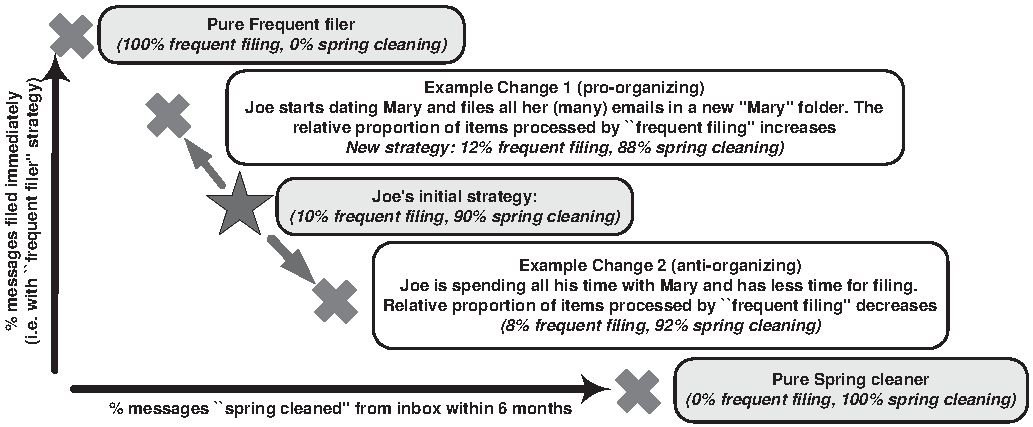
\includegraphics[width=\textwidth]{pictures/main-study/new-change-model.pdf}
	\end{center}
	\caption{A model of incremental changes in email organizing strategy}
	\label{fig:discussion:new-change-model}
\end{figure}
% CONSIDER: extending model to show both major shifts and minor shifts.}
% ADD: real examples from our study data

%%%%%%%%%%%%%%%%%%
% LIMITATIONS
%%%%%%%%%%%%%%%%%
A number of simplifying assumptions are acknowledged.  A first assumption is that all messages are filed at some point, via frequent filing or spring-cleaning.  A more realistic model would be multi-dimensional to account for other strategies, e.g. the non-filing of some messages.  Secondly, the model does not capture changes in how items are organized with a particular strategy.  For example, participant M5 moved many older project folders into a top-level `old' folder.  This does not represent a shift between strategies, but an adjustment to information that has already been filed.  Despite these simplifications, it is argued that the model provides a more realistic portrayal of changes in organizing strategy, and emphasises their incremental nature.  
% This section offers a new conceptualization of PIM strategies.  Firstly, \textbf{Section~\ref{discussion:strategies-cross-tool}} develops a cross-tool model of PIM strategy, drawing from the cross-tool perspective developed in \textbf{Section~\ref{discussion:cross-tool}}.
Furthermore, the model indicates the potential for developing improved conceptualizations of PIM strategies, and how they change over time.

% But note still abstracts the low-level manner of filing employed etc.

%%%%%%%%%%%%%%%%%%%%%%%%%%%%%%%%%%%%%%%%%%%%%%%%%%
% STUDY EXAMPLES: link changes with multiple strategies. 
%%%%%%%%%%%%%%%%%%%%%%%%%%%%%%%%%%%%%%%%%%%%%%%%%%
% In particular, it is suggested that small changes are made as demanded by new production activities and types of information.
% RELATE TO MULIPLE STRATEGIES The change data observed in the main study corresponds with the observation of \textit{multiple strategies} outlined in \textbf{Chapter~\ref{chapter:exploratory_study}}.  Multiple strategies were identified in the context of specific tools, as well as across multiple tools for most participants.

%%%%%%%%%%%%%%%%%%%%%%%%%%%%%%%%%%%%%%%%%%%%%%%%%%%%%%%%%%%%%%%%%%%%%%%%%%%%%%%%%%%%%%%%%%%%%%%%%%%%%%%%%%%%%%%%%
%%%%%%%%%%%%%%%%%%%%%%%%%%%%%%%%%%%%%%%%%%%%%%%%%%%%%%%%%%%%%%%%%%%%%%%%%%%%%%%%%%%%%%%%%%%%%%%%%%%%%%%%%%%%%%%%%
%%%%%%%%%%%%%%%%%%%%%%%%%%%%%%%%%%%%%%%%%%%%%%%%%%%%%%%%%%%%%%%%%%%%%%%%%%%%%%%%%%%%%%%%%%%%%%%%%%%%%%%%%%%%%%%%%
%%%%%%%%%%%%%%%%%%%%%%%%%%%%%%%%%%%%%%%%%%%%%%%%%%%%%%%%%%%%%%%%%%%%%%%%%%%%%%%%%%%%%%%%%%%%%%%%%%%%%%%%%%%%%%%%%

%%%%%%%%%%%%%%%%%%%%%%%%
% \subsubsection{Summary}
%%%%%%%%%%%%%%%%%%%%%%%%
%%%%%%%%%%%%%%%%%%%%%%%%%%
\subsubsection{Summary}
%%%%%%%%%%%%%%%%%%%%%%%%%%

%%%%%%%%%%%%%%%%%%%%%%%%%%%%%%%%%%
% AIM 2: FURTHER STUDY
%%%%%%%%%%%%%%%%%%%%%%%%%%%%%%%%%%
This section has discussed a number of the findings from the study component of the field trial.  Firstly, growth rates were compared between the three collections, along with the relative frequencies of the different PIM sub-activities.  The study highlighted the supporting property of PIM, and the lack of reflection on the part of users. 
The study also provided data on a number of real-life adaptations of PIM strategy.  A simple model of incremental strategy changes was proposed.
% This section highlighted the incremental nature of the observed strategy changes, and based on this data, outlined an extension to B�lter's model of strategy changes~\citep{ob:97}.   

%%%%%%%%%%%%%%%%%%%%%%%%%%%%%%%%%%%%%%%%%%%%
% MOVING ON: Towards Deeper Insights}
% Set the scene for the discussion chapter,  ...
%%%%%%%%%%%%%%%%%%%%%%%%%%%%%%%%%%%%%%%%%%%%
% \textbf{Section~\ref{main-study:discussion}} discussed the findings presented in this chapter in the context of the prior stages of this programme of research, as well as the previous work reported in \textbf{Chapter~\ref{chapter:review}}. 
Next, \textbf{Chapter~\ref{chapter:discussion}} moves on to combine the findings from this chapter with those from the wider thesis.


%%%%%%%%%%%%%%%%%%%%%%%%%%
% \subsubsection{Summary}
%%%%%%%%%%%%%%%%%%%%%%%%%%
% The study findings are used to explain design results in the next section, develop design recommendations in \textbf{Section X}, and theory in \textbf{Section Y}. % think about order ...
% This section considered longitudinal insights from the study.  These findings are used in further discussion in \textbf{Chapter~\ref{chapter:discussion}}.  

%%%%%%%%%%%%%%%%%%%%%%%%%%%%%%%%
% END: DISCUSSION - CHANGES
%%%%%%%%%%%%%%%%%%%%%%%%%%%%%%%%

%%%%%%%%%
% FIN
%%%%%%%%%


\input{tex/main-study/chapter6-main-study-DISCUSSION-strategy-changes}

% %%%%%%%%%%%%%%%%%%%%%%%%%%%
% CHAPTER 6 -- CONCLUSION
% Conclusion
% File: tex/main-study-chapter/chapter6-main-study-CONCLUSION.tex
%%%%%%%%%%%%%%%%%%%%%%%%%%%%%%%%%%%%%%%%%%%%%%%%
%%%%%%%%%%%%%%%%%%%%%%%%%%%%%%%%%%%%%%%%%%%%%%%%%%%%%%%%%%%%%%%%%%%%%%%%%%%%%%%%%%%%%%%%%%
% Richard Boardman PhD Thesis: Improving Tool Support for Personal Information Management
%%%%%%%%%%%%%%%%%%%%%%%%%%%%%%%%%%%%%%%%%%%%%%%%%%%%%%%%%%%%%%%%%%%%%%%%%%%%%%%%%%%%%%%%%%

%%%%%%%%%%%%%%%%%%%%%%%%%%%%%%%%%%%%%%%%%%%%%%%%%%%%%%%%%%%%%%%%%%%%%%%%%%%%%%%%%%%%%%%%%%
% NATBIB NOTES
%%%%%%%%%%%%%%%%%%%
%\citet{jon90}                ->    Jones et al. (1990) 
%   \citet[chap.~2]{jon90}       ->    Jones et al. (1990, chap. 2)
%   \citep{jon90}                ->    (Jones et al., 1990) 
%   \citep[chap.~2]{jon90}       ->    (Jones et al., 1990, chap. 2) 
%%%%%%%%%%%%%%%%%%%%%%%%%%%%%%%%%%%%%%%%%%%%%%%%%%%%%%%%%%%%%%%%%%%%%%%%%%%%%%%%%%%%%%%%%%


%%%%%%%%%%%%%%%%%%%%%%%%%%%%%%%
%%%%%%%%%%%%%%%%%%%%%%%%%%%%%%%
% \subsection{Conclusion}
% \label{main-study:chapter-summary}
%%%%%%%%%%%%%%%%%%%%%%%%%%%%%%%
%%%%%%%%%%%%%%%%%%%%%%%%%%%%%%%
%%%%%%%%%%%%%%
% SUMMARY
%%%%%%%%%%%%%%
% Retouch findings and contributions
%%%%%%%%%%%%%%%%%%%%%%%%%%%%%%
% This chapter has reported the objectives, method, and results of a field trial investigation into the PIM practices of eight individuals across three tools: files, email, and bookmarks. The field trial was a dual-research vehicle, aimed to satisfy two research objectives.

%%%%%%%%%%%%%%%%%%%%%%%%%%%%%%%%%%%%%%
% OVERALL SUCCESS OF THE STUDY HERE
%%%%%%%%%%%%%%%%%%%%%%%%%%%%%%%%%%%%%%
% OVERALL SUCCESS: is field study a success? Did it meet its aims?




%%%%%%%%%%%%%%%%%%%%%%%%%%%%%%%%%%%%%%%%%%%%%%%%%%%
% \textit{This draft of Chapter 6 MAIN STUDY was printed \today}
%%%%%%%%%%%%%%%%%%%%%%%%%%%%%%%%%%%%%%%%%%%%%%%%%%%%%%%%%%%%%%%%%%%%%%%%%%%%%%%%%%%%%%%%%%
%%%%%%%%%%%%%%%%%%%%%%%%%%%%%%%%%%%%%%%%%%%%%%%%%%%%%%%%%%%%%%%%%%%%%%%%%%%%%%%%%%%%%%%%%%
%%%%%%%%%%%%%%%%%%%%%%%%%%%%%%%%%%%%%%%%%%%%%%%%%%%%%%%%%%%%%%%%%%%%%%%%%%%%%%%%%%%%%%%%%%
%%%%%%%%%%%%%%%%%%%%%%%%%%%%%%%%%%%%%%%%%%%%%%%%%%%%%%%%%%%%%%%%%%%%%%%%%%%%%%%%%%%%%%%%%%




%\textit{CHAPTER 6 LEFT INTENTIONALLY BLANK AS A PLACEHOLDER}




% %%%%%%%%%%%%%%%%%%%%%%%%%%%%%%%%%%%%

% chapter 7 - Discussion

% %%%%%%%%%%%%%%%%%%%%%%%%%%%%%%%%%%%%

\chapter{Discussion}

\label{chapter:discussion}

%%%%%%%%%%%%%%%%%%%%%%%%%%%%
% CHAPTER 7 - DISCUSSION INTRO
%%%%%%%%%%%%%%%%%%%%%%%%%%%%
%%%%%%%%%%%%%%%%%%%%%%%%%%%%%%%%%%%%%%%%%%%%%%%%%%%%%%%%%%%%%%%%%%%%%%%%%%%%%%%%%%%%%%%%%%
% Richard Boardman PhD Thesis: Improving Tool Support for Personal Information Management
%%%%%%%%%%%%%%%%%%%%%%%%%%%%%%%%%%%%%%%%%%%%%%%%%%%%%%%%%%%%%%%%%%%%%%%%%%%%%%%%%%%%%%%%%%
%%%%%%%%%%%%%%%%%%%%%%%%%%%%%%%%%%%%%%%%%%%%%%%%%%%%%%%%%%%%%%%%%%%%%%%%%%%%%%%%%%%%%%%%%%
% NATBIB NOTES
%%%%%%%%%%%%%%%%%%%
%\citet{jon90}                ->    Jones et al. (1990) 
%   \citet[chap.~2]{jon90}       ->    Jones et al. (1990, chap. 2)
%   \citep{jon90}                ->    (Jones et al., 1990) 
%   \citep[chap.~2]{jon90}       ->    (Jones et al., 1990, chap. 2) 
%%%%%%%%%%%%%%%%%%%%%%%%%%%%%%%%%%%%%%%%%%%%%%%%%%%%%%%%%%%%%%%%%%%%%%%%%%%%%%%%%%%%%%%%%%
%%%%%%%%%%%%%%%%%%%%%%%%
% DISCUSSION NOTES
%%%%%%%%%%%%%%%%%%%%%%%%
% Speculate, Suggest future work
%%%%%%%%%%%%%%%%%%%%%%%%%%%%%%%%%%%%%%%%%%%%%%%%%%%%%%
% Frame as "`intermediate discussion stage"' ...
%			pulling things altogther from all over the thesis
% What it all means.  What I learned/gained
% interpret results in light of prior research/assumptions
% MUST: Link back to findings/experience
% MUST: Links forward to conclusion (e.g. future work)
%%%%%%%%%%%%%%%%%%%%%%%%%%%%%%%%%%%%%%%%%%%%%%%%%%%%%%
%%%%%%%%%%%%%%%%%%%%%%%%%%%%%%%%%%%%%%%%%%%%%%%%%%%%%%
% FRAME AS A STORY
% Consider: conflicts/changes from earlier work (e.g. consideration that integration may not be a good thing!)
% how do these insights relate/conflict to those from earlier study?. Can I frame as learning?}
% Data and discussion here appear to raise potential conflicts with earlier findings - need to think carefully about how to frame them (Angela: \textit{"`OK to admit that you learned something"'}
%%%%%%%%%%%%%%%%%%%%%%%%%%%%%%%%%%%%%%%%%%%%%%%%%%%%%%
%%%%%%%%%%%%%%%%%%%%%%%%%%%%%%%%%%%%%%%%%%%%%%%%%%%%%%
% HOWTO: What is the appropriate route to theory?
% Need justification/rationale (e.g. empirical grounding)
%�	Method of theory-building
%�	Form of theoretical deliverable
% 			Carroll's view of design/evaluation as theory building is one option (2 methods)
% 			Grounded theory analysis of main study data is another
%%%%%%%%%%%%%%%%%%%%%%%%%%%%%%%%%%%%%%%%%%%%%%%%%%%%%%
%%%%%%%%%%%%%%%%%%%%%%%%%%%%%%%%%%%%%%%%%%%%%%%%%%%%%%
% Other things to add:
% Relate ES and MS -- how did MS build on initial ES?
%	Do users see personal workspace as intrinsically different to remote spaces?}
%%%%%%%%%%%%%%%%%%%%%%%%%%%%%%%%%%%%%%%%%%%%%%%%%%%%%%

%%%%%%%%%%%%%%%%%%%%%%%%%%%%%%%%%%%%%%%%%%%%%%%%%%%%%%
%PIM SIG stages of discussion:
%\begin{itemize}
%\item What is PIM?
%\item What is PIM's current state?
%\item What is the potential of PIM?
%\item What are the challenges/obstacles of working on PIM?
%\item promising directions
%\item next steps.
%\end{itemize}
%%%%%%%%%%%%%%%%%%%%%%%%%%%%%%%%%%%%%%%%%%%%%%%%%%%%%%

%%%%%%%%%%%%%%%%%%%%%%%%%%%%%%%%%%%%%%
\section{Introduction}
\label{discussion:discussion-introduction}
%%%%%%%%%%%%%%%%%%%%%%%%%%%%%%%%%%%%%%
 
%%%%%%%%%%%%%%%
% LEAD-IN INTRO
%%%%%%%%%%%%%%%
% This section proposes theory and suggest routes for developing further theory.
%%%%%%%%%%%%%%%%%%%%%%%%%%%%%%%%
% ALT TITLE FOR CHAPTER: \section{Extending the conceptual basis of PIM}
% draws together the findings from the rest of the thesis.  
% FINDINGS -> derive -> DISCUSSION
% DEVELOPING IMPROVED MODELS OF PIM
% A series of discussions are presented that consider the findings in the light of previous work in the field
% Model/theory building from study and evaluation findings
%%%%%%%%%%%%%%%%%%%%%%%%%%%%%%%%
%%%%%%%%%%%%%%%%%%%%%%%%%%%%%%%%%%%%%%%%%%%%%%%%%%%%
% TALK ABOUT EXTENDING BARREAU'S MODEL
%%%%%%%%%%%%%%%%%%%%%%%%%%%%%%%%%%%%%%%%%%%%%%%%%%%%
% The section develops extensions of Barreau's model relating to three aspects of PIM not covered in previous work.  For each aspect, design implications and methodological implications are discussed.
%%%%%%%%%%%%%%%%%%%%%%%%%%%%%%%%%%%%%%%%%
% Some preliminary steps are taken towards developing a model of PIM encompassing three aspects of its nature as uncovered in this research programme: (1) cross-tool, (2) ongoing, and (3) supporting.
%Firstly, \textbf{Section~\ref{disc:theory-discussion}} revisits the limitations of previous theory on PIM.  Three aspects of PIM are identified as in particular need of attention: (1) the \textit{cross-tool} nature of PIM, (2) the \textit{ongoing} nature of PIM, and (3) the \textit{supporting} nature of PIM.  
%The conceptual framework outlined in Chapter 2 is extended to encompass findings from the exploratory study and main study - forming my own view of PIM
%We are extending Barreau's framework~\citep{barreau:95} to reflect the cross-tool, supporting nature of PIM.
%%%%%%%%%%%%%%%%%%%%%%%%%%%%%%%%%%
% BUILDING THEORETICAL FRAMEWORK
%%%%%%%%%%%%%%%%%%%%%%%%%%%%%%%%%%
% These theoretical perspectives are raised based on the substantive findings reported .
% e.g. extend cross-tool framework with findings from evaluation
% The framework is based on three important aspects of the nature of PIM that have been highlighted in carrying out this research.
% The three perspectives, each of which has been under-represented in earlier work, are as follows:
% Each section discusses PIM from a theoretical perspective following the experiences of the author in pursuing this programme of research.  
This chapter discusses the substantive findings from \textbf{Chapters~\ref{chapter:exploratory_study}} to \textbf{\ref{chapter:main-study}}.  The discussion is made up of the following four sections:

\begin{itemize}

\item \textbf{Section~\ref{discussion:theoretical-framework}} develops a theoretical framework which reflects three perspectives of PIM that have been highlighted over the course of this research: 1) PIM as a \textit{cross-tool} activity, (2) PIM as a \textit{supporting} activity, and (3) PIM as an \textit{ongoing} activity.   Each perspective illustrates a future direction for theory development in this area.


%%%%%%%%%%%%%%%%%%%%%%%%%%%
% DESIGN IMPLICATIONS
%%%%%%%%%%%%%%%%%%%%%%%%%%%
%%%%%%%%%%%%
% General implications/guidelines/recommendations - implications for design aimed at improving integration between PIM tools.
% Implications for design -- towards design recommendations. Can I generalise (from local findings to general design genre?) (Carroll's theory building \#1). Build model/theory out of the evaluation data (Carroll's theory building \#2)
%%%%%%%%%%%%
\item \textbf{Section~\ref{discussion:design-guidelines-discussion}} revisits the evaluation of WorkspaceMirror (WM), and uses the perspective of PIM as a supporting activity to interpret the results.  Based on this analysis, and empirical findings in the thesis, implications for the wider design genre of PIM-integration are considered. % a number of recommendations are made for the design  mechanisms.  %makes recommendations for future design work, with a particular focus on that directed at improving PIM integration.  Recommendations draw on the above theoretical discussion, and the substantive findings from earlier chapters.

%%%%%%%%%%%%%%%%%%%%%%%%%%%%%%%%%%
% METHODOLOGY IMPLICATIONS
% Methodological issues. Reflection on my experiences. 
%%%%%%%%%%%%%%%%%%%%%%%%%%%%%%%%%%
\item \textbf{Section~\ref{discussion:methodological-discussion}} presents a series of methodological recommendations for carrying out work in this area.  The framework from \textbf{Section~\ref{discussion:theoretical-framework}} is used to structure the recommendations.

%%%%%%%%%%%%%%%%%%
% MODEL OF UXP
%%%%%%%%%%%%%%%%%%
% INCLUDE TRANSITIONS FROM PEOPLE IN STUDY
% The need for improved theory in this area is highlighted in \textbf{Section~\ref{discussion:methodological-discussion}}. The next two sections propose models to explain some of the observations made in this thesis. \textbf{Section X} develops a cross-tool model of PIM strategies and how they change over time.
\item \textbf{Section~\ref{discussion:uxp}} explores possible qualitative measures of \textit{PIM user experience} that could be used as evaluation metrics.  \textbf{Section~\ref{discussion:uxp-settled}} considers one aspect of negative user experience in depth, dissatisfaction with management strategies.  The results from the main study in \textbf{Chapter~\ref{chapter:main-study}} are used to provide examples of such dissatisfaction.

%Two aspects of negative PIM user experience are discussed in depth: (1) \textit{``unsettledness'' in PIM strategy}, and (2) \textit{distraction from work activities}. % builds on the earlier discussions of PIM as an ongoing, supporting activity, to build a model of user experience over time.  The model is used to explain some of the observations made in \textbf{Chapter~\ref{chapter:main-study}}.  Suggestions are made for improved evaluation measures.

\end{itemize}

%%%%%%%%%%%%
% CONCLUSION (REQUIRED?)
%%%%%%%%%%%%
% Finally, \textbf{Section~\ref{discussion:chapter-summary}} concludes the chapter with a summary of key findings.

%%%%%%%%%%%%%%%%%%%%%%%%%%%%%%
% FIN@ CHAPTER 7 DISCUSSION INTRO
%%%%%%%%%%%%%%%%%%%%%%%%%%%%%%
















\newpage
%%%%%%%%%%%%%%%%%%%%%%%%%%%%%%%%%%%%
\section{Three Perspectives on PIM}
\label{discussion:theoretical-framework}
%%%%%%%%%%%%%%%%%%%%%%%%%%%%%%%%%%%%
% \textbf{Section~\ref{discussion:supporting}} moves on to consider PIM as a \textit{supporting} activity.  Finally, \textbf{Section~\ref{discussion:ongoing}} discusses the \textit{ongoing} nature of PIM.
%%%%%%%%%%%%%%%%%%%%%%%%%%%%%%%%%%%%%%%%%%%%%%%%%%%%%%%%%%%%%%%%%%%%%%%%%%%%%%%%%%%%%%%%%%%%%%%%%%%%%%%%%%%%
%	\item Complex activity -- and many problems.  Highly personal -- can't go to the help desk for support!!  Its your own responsibility
%%%%%%%%%%%%%%%%%%%%%%%%%%%%%%%%%%%%%%%%%%%%%%%%%%%%%%%%%%%%%%%%%%%%%%%%%%%%%%%%%%%%%%%%%%%%%%%%%%%%%%%%%%%%
%\textbf{Nature of PIM: a complex beast!!} Complex, multi-faceted area. Even with scoping, lots of data.
% Highlighted difficulty of analysis/constructing a user model/requirements and issues involved (e.g. complexity of PIM, individual Differences)
%%%%%%%%%%%%%%%%%%%%%%%%%%%%%%%%%%%%%%%%%%%%%%%%%%%%%%%%%%%%%%%%%%%%%%%%%%%%%%%%%%%%%%%%%%%%%%%%%%%%%%%%%%%%

This section discusses three properties of PIM which emerged over the course of this research:
\begin{enumerate}
%%%%%%%%%%%%%%%%%%%%%%%%%%%%%%%%%%%%%%%%%
% 2. CROSS-TOOL DISCUSSION
%%%%%%%%%%%%%%%%%%%%%%%%%%%%%%%%%%%%%%%%%
% Barreau's PIM framework~\citep{barreau:95} is extended to encompass this view of PIM.
\item \textbf{Section~\ref{discussion:cross-tool}} considers PIM as a \textit{cross-tool} activity, one which is distributed across multiple tools such as files, email and bookmarks.  

%%%%%%%%%%%%%%%%%%%%%%%%%%%%%%%%%%%%%%%%%
% 4. SUPPORTING DISCUSSION
%%%%%%%%%%%%%%%%%%%%%%%%%%%%%%%%%%%%%%%%%
% The framework from the previous section is extended to reflect the relationship between PIM and a user's production activities.
\item \textbf{Section~\ref{discussion:supporting}} discusses PIM as a \textit{supporting} activity, and considers the relationship between it and a user's production activities. 

%%%%%%%%%%%%%%%%%%%%%%%%%%%%%%%%%%%%%%%%%
% 3. ONGOING DISCUSSION
%%%%%%%%%%%%%%%%%%%%%%%%%%%%%%%%%%%%%%%%%
% Two perspectives on PIM are highlighted for analyzing PIM: (1) 
% An extension to B�lter's model of strategy changes is proposed~\citep{ob:97}.
\item \textbf{Section~\ref{discussion:ongoing}} considers the \textit{ongoing} nature of PIM, viewing it from two longitudinal perspectives: (1) as a series of discrete events, (2) as a thread of continuous activity.

\end{enumerate}

% develops a theoretical framework reflecting three aspects of the nature of PIM that emerged from this work:  (1) PIM as a \textit{cross-tool} activity, (2) PIM as a \textit{supporting} activity, and (3) PIM as an \textit{ongoing} activity.  
% The next three section considers each perspective in turn, and incrementally build up a theoretical framework based on the model proposed in~\citet{barreau:95}.  


%%%%%%%%%%%%%%%%%%%%%%%%%%%%%%%%%%%%
% COMBINATION OF PERSPECTIVES
%%%%%%%%%%%%%%%%%%%%%%%%%%%%%%%%%%%%
% A number of design and methodological implications are derived based on each theoretical perspective. In addition, a number of promising directions are identified for the attention of future research.
%  which is used to provide a commentary on the work presented in the thesis.  
% A theoretical framework is built up by extending Barreau's PIM framework to encompass these perspectives. 
% Barreau's PIM model is extended to form a theoretical framework reflecting these three themes. The framework is constructed by the incremental extension of  over the three sections. The framework is referred to in subsequent chapters of this thesis to discuss directions for future work. 
% Each section presents evidence for the view of PIM it discusses, in terms of related findings from earlier in the thesis.  
Each perspective is motivated using findings from earlier chapters, and is then used to 
incrementally extend the conceptual framework of PIM from \textbf{Section~\ref{bg:pim-activity-cf}}.  
\textbf{Section~\ref{discussion:towards-theory}} discusses how the three perspectives indicate routes for future theory development in the area.   Within this chapter, the three perspectives are used to structure the discussion in subsequent sections.  % , and also indicate potential routes for future theory development.  Indeed, it is argued that each perspective indicates an area of theory that has been under-represented in the PIM literature, and it is argued that they are of high importance to designers and researchers.


%%%%%%%%%%%%%%%%%%%%%%%%%%%%%%%%
% \subsection{Aspects of PIM}
%%%%%%%%%%%%%%%%%%%%%%%%%%%%%%%%
%%%%%%%%%%%%%%
% OHTER: Idiosyncratic
%%%%%%%%%%%%%%
% Apply: methodological recommendations, eval findings
% Individual differences illustrated by responses to tool evaluation and range of strategies.
%%%%%%%%%%%%%%%%%%%%%%%%%%%%%%%%%%%%%%%%%%%
% Identify limitations of Barreau model
%%%%%%%%%%%%%%%%%%%%%%%%%%%%%%%%%%%%%%%%%%%
%The following limitations of Barreau's model are highlighted:
%\begin{itemize}
%\item Does not reflect PIM as a \textit{cross-tool} activity 
%\item Does not reflect PIM as an \textit{ongoing} activity 
%\item Does not reflect PIM as a \textit{supporting} activity 
%\item Does not reflect PIM as an \textit{idiosyncratic} activity.
%\item Does not reflect PIM as an \textit{irrational} activity.
%\item Barreau's break-down into four sub-tasks not necessarily that clear-cut, also inter-relationship between sub-activities is unclear.  In terms of definition, importance or frequency. In actual fact, quite fuzzy. % MOVE FROM CH4
%\item Use data to derive descriptive vocabulary for talking about personal information (e.g. working/non-working versus archived, personal versus system, own versus shared). Need for improvements in descriptive terminology for talking about PIM, including types of personal information
%\end{itemize}

%%%%%%%%%%%%%%
% Irrational
%%%%%%%%%%%%%%
% EVIDENCE: Provide quotes
% DISCUSS: uestion assumptions of efficiency-based approaches and optimization in e.g. info foraging, Balter, Kirsh, 
% METH REC: usability measures, Implications for evaluation
% DESIGN RECS: Implications for ``on-demand'' PIM -- its not just about efficiency, its also how users feel

%%%%%%%%%%%%%%%%%%%%%%%%%%%%%%%%%%%%%%%%%%%%%%%%%%%%%%%%%%%%%%%%%%%%%%%%%%%%%%%%%%%%%%%%%%%%%%%%%%%%%%%%%%%%%%%%%
%%%%%%%%%%%%%%%%%%%%%%%%%%%%%%%%%%%%%%%%%%%%%%%%%%%%%%%%%%%%%%%%%%%%%%%%%%%%%%%%%%%%%%%%%%%%%%%%%%%%%%%%%%%%%%%%%
%%%%%%%%%%%%%%%%%%%%%%%%%%%%%%%%%%%%%%%%%%%%%%%%%%%%%%%%%%%%%%%%%%%%%%%%%%%%%%%%%%%%%%%%%%%%%%%%%%%%%%%%%%%%%%%%%
%%%%%%%%%%%%%%%%%%%%%%%%%%%%%%%%%%%%%%%%%%%%%%%%%%%%%%%%%%%%%%%%%%%%%%%%%%%%%%%%%%%%%%%%%%%%%%%%%%%%%%%%%%%%%%%%%


%%%%%%%%%%%%%%%%%%%%%%%%%%%%
% CHAPTER 7 - DISCUSSION of THEORY: CROSS-TOOL
%%%%%%%%%%%%%%%%%%%%%%%%%%%%
%%%%%%%%%%%%%%%%%%%%%%%%%%%%%%%%%%%%%%%%%%%%%%%%%%%%%%%%%%%%%%%%%%%%%%%%%%%%%%%%%%%%%%%%%%
% Richard Boardman PhD Thesis: Improving Tool Support for Personal Information Management
%%%%%%%%%%%%%%%%%%%%%%%%%%%%%%%%%%%%%%%%%%%%%%%%%%%%%%%%%%%%%%%%%%%%%%%%%%%%%%%%%%%%%%%%%%
% Towards a more realistic/alternative cross-tool model of today's workspace and user's PIM activity to understand/discuss -- parallel management of multiple PIM systems.  A new way of seeing problem/ a new perspective. Raises both opportunities and challenges. 

%%%%%%%%%%%%%%%%%%%%%%%%%%%
\subsection{PIM as a Cross-tool Activity}
\label{discussion:cross-tool}
%%%%%%%%%%%%%%%%%%%%%%%%%%%
%%%%%%%%%%%%%%
% CROSS-TOOL
%%%%%%%%%%%%%%
%\textbf{Definition of workspace. Starting analytical scope.}
%		\item Space as environment
%		\item Physical and digital
%		\item Relate to Kirsh's work context
%		\item Location for production and supporting activities
%%%%%%%%%%%%%%%%%%%%%%%%%%%%%%%%%%%%%%%%%%%%%%%%%%%%%%%%%%%%%%%%%%%%%%%%%%%%%%%
%		\item Abstract PIM system. DIAGRAM (as in Kaptelinin)
%		\item Here the computer as a PIM system cf. specific tools as PIM systems
%%%%%%%%%%%%%%%%%%%%%%%%%%%%%%%%%%%%%%%%%%%%%%%%%%%%%%%%%%%%%%%%%%%%%%%%%%%%%%%
% Workspace as a cross-tool artifact to support cross-tool PIM activity (THINK: how would Carroll talk about it all?). Feature as an artifact? (REF: Raskin) From PIM-tool as habitat to workspace as habitat
% HOW TO FRAME AS INITIAL FOCUS?
% -- since tools are inter-related
% Evidence: problems, activities are cross-tool (from chapter 4)
%%%%%%%%%%%%%%%%%%%%%%%%%%%%%%%%%%%%%%%%%%%%%%%%%%%%%%%%%%%%%%%%%%%%%%%%%%%%%%%
% Firstly, evidence from earlier chapters is presented to support this view.  Then, Barreau's model of PIM~\citep{barreau:95} is extended to encompass the cross-tool nature of PIM.  This model is contrasted with related theoretical views. Building on the model presented in \textbf{Section~\ref{discussion:cross-tool:activity-model}}, a model of PIM strategies is proposed to reflect the empirical findings reported in \textbf{Chapters~\ref{chapter:exploratory_study}} and \textbf{\ref{chapter:main-study}}.  Finally, implications for design and methodology are discussed. Two analytical perspectives are discussed, the computer workspace as (1) a single PIM artefact, and (2) a set of parallel PIM artefacts.  

%%%%%%%%%%%%%
% OVERVIEW
%%%%%%%%%%%%%
% This section discusses PIM from the first of three theoretical perspectives: that of PIM as a \textit{cross-tool} activity (one that involves multiple tools).

%%%%%%%%%%%%%%%%
% EVIDENCE
%%%%%%%%%%%%%%%%
%%%%%%%%%%%%%%%%%%%%%%%%%%%%%%%%%%%%%%%%%%%%%%
%\subsection{Evidence for cross-tool view}
%\label{discussion:cross-tool:evidence}
%%%%%%%%%%%%%%%%%%%%%%%%%%%%%%%%%%%%%%%%%%%%%%
% FOUNDATION: cross-tool data, evidence of PIM CT problems etc.
% Highlight findings from Literature Review and exploratory study that motivate/justify this approach.
% Information Management and Task Management are distributed. DIAGRAM.
Today's computing environments allow users to manage information in a variety of PIM-tools.  However, as noted in \textbf{Chapter~\ref{chapter:review}}, most previous PIM studies have focused on specific tools such as files or email.  In contrast, this research employed a deliberately cross-tool approach to investigate ways of improving integration between PIM-tools.  A focus was taken on three PIM-tools: files, email and bookmarks.  Almost all of the study participants from \textbf{Chapters~\ref{chapter:exploratory_study}} and \textbf{\ref{chapter:main-study}} actively managed all three PIM-tools.  The observations of \textit{folder overlap} indicate the information relating to a particular activity was fragmented across PIM-tools.  In other words. multiple PIM-tools were involved in certain user activities.  Also, the management of information in a particular technological format (e.g. files), was \textit{compartmentalized} across different PIM-tools.

These observations lead the author to conceptualize PIM as a \textit{cross-tool} activity, one that is distributed across multiple tools.  Previous tool-specific research in the context of email, has considered how the collection of messages acts as a \textit{``habitat''} for user activities~\citep{Ducheneaut:01}.  In contrast, this section considers PIM from a cross-tool perspective, whereby email is one component of the wider habitat of the user's personal information environment. %a user's cross-tool activity space. 

% A key driver behind this thesis work was to investigate PIM from a crss-tool perspective, and in particular to investigate the potential to improve integration between PIM-tools.  The research focused on three commonly-employed PIM-tools: files, email and bookmarks.
% The observation of folder overlap in \textbf{Section~\ref{exp-study:Results-folder-overlap}} indicate that multiple PIM-tools are utilised in specific user activities and roles.  
% Therefore, the view is taken that PIM is 
% \textbf{Chapter~\ref{chapter:exploratory_study}} reports a cross-tool study. \textbf{Chapter~\ref{chapter:design}} outlines the design of WorkspaceMirror (WM), a mechanism to integrate how information is organized in three PIM-tools.  \textbf{Chapter~\ref{chapter:main-study}} reports a second cross-tool study centred on the evaluation of the WM prototype. % REFER TO OTHER RELATED WORK/FINDINGS.
%%%%%%%%%%%%%%%%%%%%%%%%%%%%%%
% \subsubsection{Related work}
% \label{discussion:cross-tool:related-theory}
%%%%%%%%%%%%%%%%%%%%%%%%%%%%%%
% Evidence from studies of cross-tool'ness, problems etc. (Blandford and Green (harmonious co-mingling), Bellotti)
% Based on findings from literature review and my own data/experience.  Theoretical motivation, similar stances:
Various strands of related research come together in supporting this perspective.
%%%%%%%%%%%
% KIRSH
%%%%%%%%%%%
% Distributed Cognition (space/people, time, internal/external). Kirsh's view of work context ~\cite{dk:00}. Computer as an activity space containing resources and constraints
In terms of theory, the view draws on the conceptualization of a computer as an \textit{activity space}, populated by the tools and resources that facilitate action, and the constraints that limit it~\citep{dk:01}. From this theoretical perspective, activities such as PIM, are not confined to specific tools, but are distributed across a range of tools throughout digital activity space.
%%%%%%%%%%%%%%%%%%%%%%%%
% BLANDFORD AND GREEN
%%%%%%%%%%%%%%%%%%%%%%%%
Recent empirical work has also highlighted how the management of certain types of information is fragmented across multiple PIM-tools, e.g. to-dos and appointments~\citep{bg:01,Bellotti:00}, bookmarks~\citep{kftf:01}, and contacts~\citep{Whittaker-contacts:02}.  % \citet{bg:01} offer the term \textit{ensemble} to describe the set of tools that task and time management are distributed across.


%%%%%%%%
% BELLOTTI ET AL.
%%%%%%%%
% In order to provide effective support for such cross-tool activities, integration between tools is crucial. However there is evidence that this issue is not being given enough attention by designers. Bellotti and Smith (2000) note the compartmentalization of PIM activities due to poor integration between tools. For example, document collections are often divided between those stored in the file system and those stored as email attachments.
%%%%%%%%%%%%%%%%%%%%%%%%%%%%%%%%%%%%%%%%%%%%%%%%%%%%%%%%
% USE ME:In terms of the theoretical framework offered by Kirsh, compartmentalization may be considered as one set of constraints imposed on a user's activity space by poorly designed tools.
%%%%%%%%%%%%%%%%%%%%%%%%%%%%%%%%%%%%%%%%%%%%%%%%%%%%%%%%
%%%%%%%%
% DIX
%%%%%%%%
%\textit{Dix ~\cite{dix:98} (but focus on coordinating)}
%%%%%%%%%%%%%%%%%%%%%%%%%%%%%%%%%%%%%%%%%%%%%%%%%%%%%%%%
%%%%%%%%%%%%%%%%%
% KAPTELININ
%%%%%%%%%%%%%%%%%
%\textit{Kaptelinin~\citep{Kaptelinin:96,Kaptelinin:03} -- model of PIM activity}
%%%%%%%%%%%%%%%%%%%%%%%%%%%%%%%%%%%%%%%%%%%%%%%%%%%%%%%%
%%%%%%%%%%%%
% Raskin
%%%%%%%%%%%%
%\textit{Relate to Raskin. Content as content with standard operations.}
%\textit{Here, it is argued that PIM support is a cross-tool feature set.  Unified amalgam of all PIM functionality.}
%%%%%%%%%%%%%%%%%%%%%%%%%%%%%%%%%%%%%%%%%%%%%%%%%%%%%%%%
%%%%%%%%%%%%%%%%%%%%%%%%%%%%%%%%%%%%%%%%%%
% What are limitations of this theory?
% i.e. why am I even trying to do this?
%%%%%%%%%%%%%%%%%%%%%%%%%%%%%%%%%%%%%%%%%%
%\textit{What is wrong with existing models/are there any?}
%%%%%%%%%%%%%%%%%%%%%%%%%%%%%%%%%%%%%%%%%%%%%%%%%%%%%%%%

%%%%%%%%%%%%%%%%%%%%%%%%%%%%%%%%%%%%%%%%%%%%%%%%%%%%%%%%%%%%%%%%%%%%%
\subsubsection{Extending the Conceptual Framework from Chapter 2}
%%%%%%%%%%%%%%%%%%%%%%%%%%%%%%%%%%%%%%%%%%%%%%%%%%%%%%%%%%%%%%%%%%%%%

%%%%%%%%%%%%%%%%%%%%%%
% BUILD ON BARREAU
%%%%%%%%%%%%%%%%%%%%%%
% However here it is argued that such an abstract view does not accurately reflect the nature of the PIM carried out by today's users.
% Now want to shift boundaries based on a new analytical perspective.  Idea of a model which tool designers can refer to. Or better as just simple recommendations?
% The workspace as a PIM-tool.  PIM as a cross-tool activity. 
% Here we go -- a Cross-Tool Analytical Proto-Model of Cross-tool PIM}:
% Cue cross-tool model of workspace (REF: a la Victor's model) 
% Barreau's framework~\citep{barreau:95} is extended to reflect the workspace as a high-level PIM system, containing lower-level PIM systems within distinct tools.  
% \textbf{Chapter~\ref{chapter:bg}} provided a brief introduction to Barreau's model of PIM, consisting of four sub-activities: acquisition, organization, maintenance and retrieval.
\textbf{Chapter~\ref{chapter:bg}} presented a conceptual framework of four PIM sub-activities: acquisition, organization, maintenance and retrieval. This was based on ~\citet{barreau:95} who models the computer as a \textit{single PIM system}.  % However, as discussed above, today's computers offer the facility to manage multiple collections of information, based on distinct technological formats, within different PIM-tools.
Here it is argued that another more accurate conceptualization of a personal computer is as a \textit{set of distinct PIM-systems}\footnote{Barreau's abstraction of the computer as a single PIM system may be due to the fact that her work was focused on the file system, and furthermore was carried out in 1995.  Other PIM-tools, such as email and web browsers were not as common then as now. Indeed, Barreau notes that only two of her eight participants managed email.}.
%%%%%%%%%%%%%%%
% NEW MODEL
%%%%%%%%%%%%%%%
\textbf{Figure~\ref{fig:discussion:PIM-cross-tool-model}} illustrates the extension of Barreau's framework to reflect this view.  PIM can therefore be viewed from two perspectives as follows:
%The primary reason for the limitations of Barreau's model is that her study focused on one tool: the file system.  The author acknowledges that this is an understandable limitation, since in 1995, .  % Indeed in 1995, when her study was reported, few participants employed email, and web browsers were not common.  Barreau conceptualized the computer as a single abstract PIM system, whereas from our data it is clear that current PIM-tools constitute a set of parallel yet inter-related systems. We also seek to modify the framework to capture the influence of production tasks in determining PIM needs.

\begin{enumerate}

%%%%%%%%%%%%%%%%%%%%%%%
% UNIQUE SUB-SYSTEMS
%%%%%%%%%%%%%%%%%%%%%%%
%Each tool allows the user to manage a specific type of information, in other words they amount to a specific PIM-system.  
% Why do we need to consider different aspects of each PIM sub-system?
% PIM has unique qualities in some tools.  In other words, PIM as an abstract activity that is instantiated in multiple PIM tools, possibly in slightly different ways. Some information in tools is self-contained. Other aspects overlap.
\item Firstly, from a \textit{tool-specific} perspective, each PIM-tool can be considered as a distinct PIM system which provides the functionality to acquire, organize, maintain and retrieve information based on a specific technological format. Although different PIM-tools share commonalities, they also have many unique aspects. \textbf{Chapter~\ref{chapter:exploratory_study}} surveyed how the nature of the PIM sub-activities varied across files, email and bookmarks. % could use example of acquisition here

%%%%%%%%%%%%%%%%%
% INTEGRATION and link to next section
%%%%%%%%%%%%%%%%%
Linking the independent ``PIM-subsystems'' are \textit{integration mechanisms}, such as email attachment functionality, and the WM prototype proposed in \textbf{Chapter~\ref{chapter:design}}.

%%%%%%%%%%%%%%%%%%%%%%%%%%%%%%%%%%%%%%%
% HL global system
% Set of sub-systems
% I.e. look beyond individual tools. 
%%%%%%%%%%%%%%%%%%%%%%%%%%%%%%%%%%%%%%%
% If to consider the computer as single PIM system, it must be recognised that it is made up of multiple PIM sub-systems. Different PIM-tools contribute together to high-level PIM support afforded by the workspace as a whole.  Treat as workspace-wide phenomena/workspace-level. Represents change from application-centric view
% Multiple PIM sub-systems that amount together to a computer-wide PIM-system.   
% Acquisition into ``global PIM system'' is net effect of all the parallel tool-specific acquisition.  Sources of PI: self-created, sent/pushed, actively seeking/foraged).
\item Secondly, from a \textit{cross-tool} perspective, the entire desktop computer can be considered as one federated PIM system composed of the set of tool-specific PIM sub-systems.  From a cross-tool perspective, the acquisition sub-activity is the sum of all the tool-specific acquisition processes, including email messages received from other people, and files and bookmarks created by the user.

\end{enumerate}  


% %%%%%%%%%%%%%%%%%%%%%%%%%%%%%
% FIGURE - Cross-tool ACTIVITY model of PIM
% %%%%%%%%%%%%%%%%%%%%%%%%%%%%%
%%%%%%%%%%%%%%%%%%%%%%%%%%%%%%
\begin{figure}[htbp]
	\begin{center}
		\leavevmode
		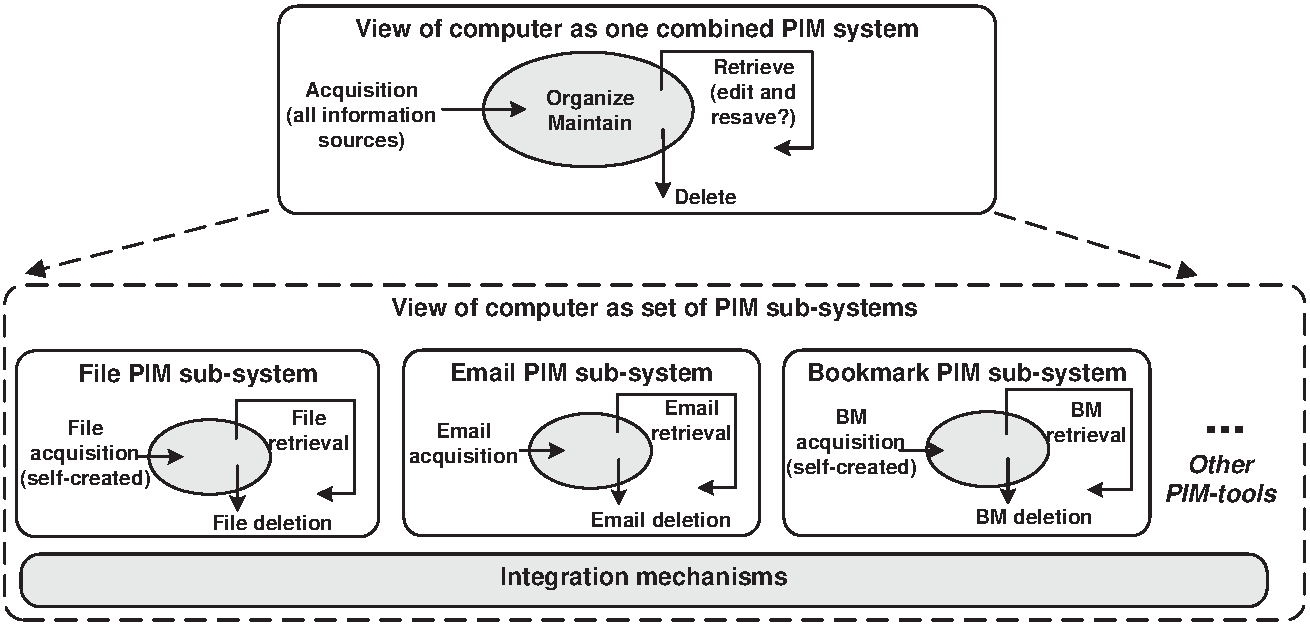
\includegraphics[width=\textwidth]{pictures/discussion/PIM-cross-tool-model.pdf}
		% fs-fm-comparison.pdf}
	\end{center}
	\caption{An extension of Barreau's PIM framework to reflect the cross-tool perspective}
	\label{fig:discussion:PIM-cross-tool-model}
\end{figure}



%%%%%%%%%%%%%%%%%%%%%%%
% TIP OF THE ICEBERG
%%%%%%%%%%%%%%%%%%%%%%%
% But also can consider far beyond the desktop
% Need to think beyond desktop as well - what about extended workspace?  
% There are many others, for example on the desktop, calendars, remote file stores and to-do-lists.  There are also other devices that should be considered, although outside the scope of this research programme.
% Note that the figure only includes three example PIM-tools, there are many more. One can also imagine a more extensive abstract view of the extended personal information environment.
\textbf{Figure~\ref{fig:discussion:PIM-cross-tool-model}} is limited to a focus on three PIM-tools: files, email and bookmarks.  However, these three are intended as indicative examples only.  Other PIM-tools could be included such as calendars and to-do lists.  Future extensions could also consider the extended personal information environment beyond the desktop -- shared drives, web-based information, as well as information stored on other devices and in the physical environment.  For now, the point to be taken by the reader is that PIM can be considered as a cross-tool activity.
% Also, many other tools have PIM facilities, even tools not really thought of as PIM tools.  


%%%%%%%%%%%%%%%%%%%%%%%%%%%%%
% LINK TO NEXT SECTIONS
%%%%%%%%%%%%%%%%%%%%%%%%%%%%%
% Before moving onto design implications,
The key benefit of the extended framework is that it allows the accommodation of cross-tool integration mechanisms.
\textbf{Section~\ref{discussion:supporting}} moves on to further develop the framework in \textbf{Figure~\ref{fig:discussion:PIM-cross-tool-model}} to encompass the relationship between PIM and the production tasks that it supports.

%%%%%%%%%%%%%%%%%%%%%
% FIN: CROSS-TOOL
%%%%%%%%%%%%%%%%%%%%%









%%%%%%%%%%%%%%%%%%%%%%%%%%%%
% CHAPTER 7 - DISCUSSION of THEORY: SUPPORTING
%%%%%%%%%%%%%%%%%%%%%%%%%%%%
%%%%%%%%%%%%%%%%%%%%%%%%%%%%%%%%%%%%%%%%%%%%%%%%%%%%%%%%%%%%%%%%%%%%%%%%%%%%%%%%%%%%%%%%%%
% Richard Boardman PhD Thesis: Improving Tool Support for Personal Information Management
%%%%%%%%%%%%%%%%%%%%%%%%%%%%%%%%%%%%%%%%%%%%%%%%%%%%%%%%%%%%%%%%%%%%%%%%%%%%%%%%%%%%%%%%%%
%%%%%%%%%%%%%%%%%%%%%%%%%%%%%%%%
% DISCUSS: relate to satisficing nature 
%%%%%%%%%%%%%%%%%%%%%%%%%%%%%%%%
% ~\cite{barreau:95} notes the \textit{satisficing} nature of PIM. However there is more at play here. It is not just a lack of time, which infers some satisficing decision as directed by efficiency constraints}
%%%%%%%%%%%%%%%%%%%%%%%%%%%%%%%%
% Supporting nature beyond satisficing: distraction, futzing, discretional
%%%%%%%%%%%%%%%%%%%%%%%%%%%%%%%%
% Also a lack of inclination, they are discretionary and may not even be necessary at all.  However in some cases the user will perform them anyway}
%%%%%%%%%%%%%%%%%%%%%%%%%%%%%%%%
% cognitive work activities
%%%%%%%%%%%%%%%%%%%%%%%%%%%%%%%%
% \textit{DISCUSS: cognitive work activities}
%%%%%%%%%%%%%%%%%%%%%%%%%%%%%%%%
% information foraging
%%%%%%%%%%%%%%%%%%%%%%%%%%%%%%%%
% Contrast with Pirolli and Card's embedding of information foraging within context of another task
%%%%%%%%%%%%%%%%%%%%%%%%%%%%%%%%
% Production tasks++
%%%%%%%%%%%%%%%%%%%%%%%%%%%%%%%%
% {Not just production tasks, also emotional needs, e.g lets keep those pictures as they are nice and maybe I will want to see them again. But also consider irrational aspects. What if no production activity?
%%%%%%%%%%%%%%%%%%%%%%%%%%%
% Link to ongoing theme
%%%%%%%%%%%%%%%%%%%%%%%%%%%
% \item Not a single goal, in fact a multiplicity of shifting short-term/long-term goals as driven by production tasks.  Need to juggle to prioritize?  \textit{How to measure user costs overall? Impact on methodology. LINK to method section below}




% \newpage
%%%%%%%%%%%%%%%%%%%%%%%%%
% SUPPORTING/REFLECTION
% Lack of reflection}
%%%%%%%%%%%%%%%%%%%%%%%%%
%%%%%%%%%%%%%%%%%%%%%%%%%%%%%%%%%%
\subsection{PIM as a Supporting Activity}
\label{discussion:supporting}
%%%%%%%%%%%%%%%%%%%%%%%%%%%%%%%%%%
% Relationship of PIM with production activities
% Provide examples of production activities
% Relationship between PIM and production activities and other supporting activities (e.g. brainstorming)
% Acceptance of problems, get worse in background (USE IN LONGIT/USER EXPERIENCE/REFLECTION)
% Paradox of the supporting tool.  Trying to improve a tool that distracts people from what they're meant to be doing! (USE IN THEORY DEV: BALANCE MODEL)
%%%%%%%%%%%%%%%%%%%%%%%%%%%%%%%%%%

%%%%%%%%%%%%%%%%%%%%%%%%%%%%%%%%
% \subsubsection{ONTO SUPPORTING}
%%%%%%%%%%%%%%%%%%%%%%%%%%%%%%%%

%%%%%%%%%%%%%%%%%%%%%%%%%
% LINK TO NEXT SECTION
%%%%%%%%%%%%%%%%%%%%%%%%%
%%%%%%%%%%%%%%%%%%%%%%%%%%%%%%%%%%%%%%%%%%%%%%%%
% Consider cross-tool supporting activities
%%%%%%%%%%%%%%%%%%%%%%%%%%%%%%%%%%%%%%%%%%%%%%%%
% FOR EXAMPLE: need for coordination. Overheads of coordinating tools together
% Cross-tool \textit{production activities} involving multiple PIM-tools, evidenced by folder overlap
%%%%%%%%%%%%%%%%%%%%%%%%%%%%%%%%%%%%%%%%%%%%%%%%%%%%%%%%%%%%%%%%%%%%%%%%%%%%%%%%%%%%%%%%%%%%%%%%%%%%%%%%%%%%%%%%%
%In many cases, multiple PIM-tools are involved in managing information in support of common production activities (\textit{Need to define production/supporting activities}).  This phenomenon is confirmed by the observations of \textit{folder overlap} in \textbf{Chapter~\ref{chapter:exploratory_study}}.  For such activities, users must also encounter overheads due to coordinating related information resources across multiple collections.
%%%%%%%%%%%%%%%%%%%%%%%%%%%%%%%%%%%%%%%%%%%%%%%%%%%%%%%%%%%%%%%%%%%%%%%%%%%%%%%%%%%%%%%%%%%%%%%%%%%%%%%%%%%%%%%%
%\textbf{Section~\ref{discussion:supporting}} discusses the relationship between PIM and the production tasks that it supports.  The section highlights that inter PIM-tool integration is particularly important when a multiple PIM-tools are involved in a particular production task.
%%%%%%%%%%%%%%%%%%%%%%%%%%%%%%%%%%%%%%%%%%%%%%%%%%%%%%%%%%%%%%%%%%%%%%%%%%%%%%%%%%%%%%%%%%%%%%%%%%%%%%%%%%%%%%%%%
%The next section moves on to consider the \textit{supporting} nature of PIM, and to discuss optimal routes for designing integration mechanisms.
%%%%%%%%%%%%%%%%%%%%%%%%%%%%%%%%%%%%%%%%%%%%%%%%%%%%%%%%%%%%%%%%%%%%%%%%%%%%%%%%%%%%%%%%%%%%%%%%%%%%%%%%%%%%%%%%%
%It is argued that current PIM-tools do not provide good support for cross-tool production activities.
%%%%%%%%%%%%%%%%%%%%%%%%%%%%%%%%%%%%%%%%%%%%%%%%%%%%%%%%%%%%%%%%%%%%%%%%%%%%%%%%%%%%%%%%%%%%%%%%%%%%%%%%%%%%%%%%%
% \textbf{Section~\ref{discussion:cross-tool}} discussed the \textit{cross-tool} nature of PIM.
% This section considers PIM from a second theoretical perspective: that of PIM as a \textit{supporting} task, one that is performed by a user in support of their production goals.
% A number of empirical findings from the studies reported in previous chapters highlight the supporting nature of PIM.
% The supporting nature of PIM is highlighted by the following quote from participant M6 in the main study reported in : . Similar paradoxical views were reported by several participants in the study: that PIM is a necessary activity, but one that is equally unimportant.
% This indicates a paradoxical situation, whereby participants were driven to manage their information, yet ran the risk of wasting time in doing so.
%%%%%%%%%%%%%%%%%%%%%%%%%%%%%%%%%%%%%%%%%%%%%%%%%%%%%%%%%%%%%%%%%%%%%%%%%%%%%%%%%%%%%%%%%%%%%%%%%%%%%%%%%%%%%%%%%
% When asked how their time could be better spent, participants typically responded that they should be doing ``real work'' rather than managing files or email.
%%%%%%%%%%%%%%%%%%%%%%%%%%%%%%%%%%%%%%%%%%%%%%%%%%%%%%%%%%%%%%%%%%%%%%%%%%%%%%%%%%%%%%%%%%%%%%%%%%%%%%%%%%%%%%%%%
% Participant F2 identified ``writing papers'' as what he should be doing rather than managing files.
% PIM was often seem as an escape or a therapeutic break from work.
% Yet users are clearly driven to carry out PIM in some form on a regular basis, if as nothing more than a break from ``real work''. % ADD QUOTE.
%%%%%%%%%%%%%%%%%%%%%%%%%%%%%%%%%%%%%%%%%%%%%%%%%%%%%%%%%%%%%%%%%%%%%%%%%%%%%%%%%%%%%%%%%%%%%%%%%%%%%%%%%%%%%%%%%
% Lack of reflection - emphasised background nature of PIM.
% lack of reflection (how tool and study in general prompted reflection).  
% The longitudinal study also highlighted the \textit{lack of attention} many users devote to PIM.  
%%%%%%%%%%%%%%%%%%%%%%%%%%%%%%%
% PROMOTION OF REFLECTION
%%%%%%%%%%%%%%%%%%%%%%%%%%%%%%%
% Participants suggested that both the study and tool interventions increased
% the amount of time they devoted to reflecting on PIM. 
% \textit{Self-auditing effect:	Need to delete that, that's where that is}
% All participants in the main study indicated that their participation, combined with the design intervention, lead them to devote more attention to PIM.  For example, during the interviews many participants performed tidying of their file, email and bookmark collections -- the interviews had a clear ``self-auditing'' effect.
%%%%%%%%%%%%%%%%%%%%%%%%%%%%%%%%%%%%%%%%%%%%%%%%%%%%%%%%%%%%%%%%%%%%%%%%%%%%%%%%%%%%%%%%%%%%%%%%%%%%%%%%%%%%%%%%%
%%%%%%%%%%%%%%%%%%%%%%%%%%%%%%%%%%%%%%%%%%%%%%%%%%%%%%%%%%%%%%%%%%%%%%%%%%%%%%%%%%%%%%%%%%%%%%%%%%%%%%%%%%%%%%%%%
%%%%%%%%%%%%%%%%%%%%%%%%%%%%%%%%%%%%%%%%%%%%%%%%%%%%%%%%%%%%%%%%%%%%%%%%%%%%%%%%%%%%%%%%%%%%%%%%%%%%%%%%%%%%%%%%%
%%%%%%%%%%%%%%%%%%%%%%%%%%%%%%%%%%%%%%%%%%%%%%%%%%%%%%%%%%%%%%%%%%%%%%%%%%%%%%%%%%%%%%%%%%%%%%%%%%%%%%%%%%%%%%%%%

%%%%%%%%%%%%%%%%%%%%%%%%%%%
% \subsubsection{Evidence for this view}
%%%%%%%%%%%%%%%%%%%%%%%%%%%%%%%%
% FOUNDATION: supporting data
%%%%%%%%%%%%%%%%%%%%%%%%%%%%%%%%
% The author developed this view during the empirical work reported in \textbf{Chapters~\ref{chapter:exploratory_study}} and \textbf{\ref{chapter:main-study}}.
In both studies participants reported that the interviews caused them to spend a lot more time thinking about PIM than normal.  Although they carried out PIM everyday, PIM was not an activity that most reported spending time focused on.  In the main study, when asked about their PIM practices regarding files, email and bookmarks, PIM was portrayed as a necessary activity, yet one that was not considered to be ``real work'' (see \textbf{Section~\ref{main-study:results:reflection}}).  In fact, a number of participants saw PIM as a chance for a welcome break, or as a waste of time! %, \textit{M6: ``There is never enough time to do PIM, and whatever time you do spend on it is often wasted''}.

%%%%%%%%%%%%%%%%%%%%%%%%%%%%%%%%%%%%%%%%%%%%%%%%
% ARGUE THAT PIM IS SUPPORTING BASED ON THIS
% Instead users are focused on production goals.  
%%%%%%%%%%%%%%%%%%%%%%%%%%%%%%%%%%%%%%%%%%%%%%%%
These results support the conceptualization of PIM as a \textit{supporting} activity.  This section suggests that it is a user's high-level production activities and goals, their ``real work'', that provide direction to their otherwise discretionary PIM activity.  The next section extends the theoretical framework from \textbf{Section~\ref{discussion:cross-tool}} to encompass this view.

%%%%%%%%%%%%%%%%%%%%%%%%%%%%%%%%%%%%%%%%%%%%%%%%%%%%%%%%%%%%%%%%%%%%%%%%%%%%%%%%%%%%%%%%%%%%%%%%%%%%%%%%%%%%%%%%%
%%%%%%%%%%%%%%%%%%%%%%%%%%%%%%%%%%%%%%%%%%%%%%%%%%%%%%%%%%%%%%%%%%%%%%%%%%%%%%%%%%%%%%%%%%%%%%%%%%%%%%%%%%%%%%%%%
%%%%%%%%%%%%%%%%%%%%%%%%%%%%%%%%%%%%%%%%%%%%%%%%%%%%%%%%%%%%%%%%%%%%%%%%%%%%%%%%%%%%%%%%%%%%%%%%%%%%%%%%%%%%%%%%%
%%%%%%%%%%%%%%%%%%%%%%%%%%%%%%%%%%%%%%%%%%%%%%%%%%%%%%%%%%%%%%%%%%%%%%%%%%%%%%%%%%%%%%%%%%%%%%%%%%%%%%%%%%%%%%%%%
% The next section extends the theoretical framework proposed \textbf{Section~\ref{discussion:cross-tool}} to describe this relationship.

%%%%%%%%%%%%%%%%%%%%%%%%%%%%%%%%%
\subsubsection{Production and Supporting Activities}
%%%%%%%%%%%%%%%%%%%%%%%%%%%%%%%%%
% Finally, the study highlighted the supporting nature of PIM. Here, several avenues are suggested for modifying the framework to capture the influence of an individual's production tasks in determining their PIM needs.
% In this section, a theoretical framework is developed to differentiate PIM and the production activities it supports.
Based on the above discussion, two types of activity are introduced:

\begin{enumerate}

%%%%%%%%%%%%%%%%%%%%%%%%%%%%%%%%%%%
% Define production activities
%%%%%%%%%%%%%%%%%%%%%%%%%%%%%%%%%%%
\item \textit{Production activities} are defined as the ``high-level'' work and leisure activities which drive a user's computer usage.  In a work context, these are the activities on which the user's performance is appraised. For example, a lawyer's production activities may include presenting court cases and writing wills for clients.  For a student, production activities may include completing coursework and revising for exams.

%%%%%%%%%%%%%%%%%%%%%%%%%%%%%%%%%%%%
% Define supporting activities
%%%%%%%%%%%%%%%%%%%%%%%%%%%%%%%%%%%%
% Must be careful - more to PIM drive than production task
\item \textit{Supporting activities} are performed to promote the completion of production activities.  In other words, they are not carried out for their own sake, instead they are ``the things one does to get something else done''.  PIM, the focus of this thesis, is a key supporting activity.  It is argued that PIM is not the primary reason people use computers.  Instead, it is performed to support their production activities.

\end{enumerate}

%%%%%%%%%%%%%%%%%%%%%%%%%%%%%%%%%%%%%%
% SUPPORTING ACTIVITIES IN GENERAL
%%%%%%%%%%%%%%%%%%%%%%%%%%%%%%%%%%%%%%
% There may be a hierarchy of production/supporting relationships
% This thesis focuses on personal information management as one supporting activity, but there are clearly many others.
% The relationship between the supporting activities involved in the example production activity of writing a report is  illustrated in
Production activities may involve multiple supporting activities.  \textbf{Figure~\ref{fig:design:PIM-production-rship-multsupp}} illustrates the supporting activities driven by an example production activity, that of writing a confidential report. These include the management of files, email, and bookmarks, communication with colleagues, updating software applications, and effective IT security practice (e.g. choosing a good password, and locking the screen).  % WHERE TO PLACE: DISCUSS DISCRETIONARY IN DEPTH
There may also be a nested arrangement of production/supporting relationships.  For example, email-based PIM can be seen as an activity that supports collaboration with co-authors, which in turn supports the overall production goal of writing the report.

In a work context, some supporting activities, such as security awareness may be enforced through guidelines.  The others shown in \textbf{Figure~\ref{fig:design:PIM-production-rship-multsupp}}, including PIM, are important, but \textit{discretionary}. Typically, the employee is not directly appraised regarding their execution. In fact, PIM is often the personal responsibility of the employee who can choose whether and to what extent they perform it.  This \textit{discretionary} nature of PIM has both positive and negative consequences.  Users are given the freedom to manage information as they choose, and may well have strong views about how to do so.  However, users typically receive little help from employers regarding the problems they encounter.





% %%%%%%%%%%%%%%%%%%%%%%%%%%%%%
% FIGURE - Relationship between supporting activities and production activities
% %%%%%%%%%%%%%%%%%%%%%%%%%%%%%
%%%%%%%%%%%%%%%%%%%%%%%%%%%%%%
\begin{figure}[htbp]
	\begin{center}
		\leavevmode
		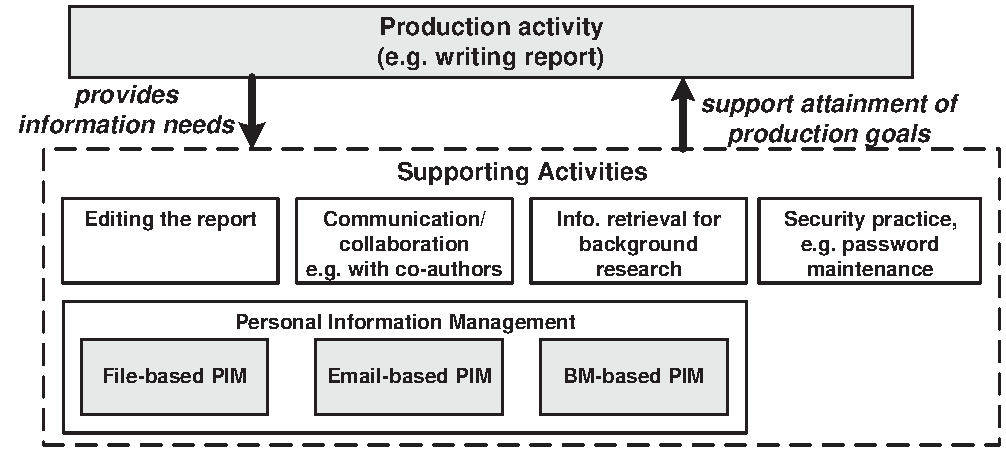
\includegraphics[height=6cm]{pictures/discussion/PIM-production-rship-multsupp.pdf}
		% fs-fm-comparison.pdf}
	\end{center}
	\caption{Supporting activities involved in the production activity of writing a report}
	\label{fig:design:PIM-production-rship-multsupp}
\end{figure}

%%%%%%%%%%%%%%%%%%%%%%%%%%%%%%%%%
% CONTRAST WITH WORK/ENABLING
%%%%%%%%%%%%%%%%%%%%%%%%%%%%%%%%%
The production/supporting relationship can be contrasted with a previous conceptualization of \textit{work} and \textit{enabling} tasks~\citep{Whitefield:93}.  Enabling tasks are tasks that are \textit{required to achieve a work goal}. For example, the enabling task of ``pressing a key'' helps achieve the work goal of ``typing a sentence in a report''.  In contrast, the supporting activities outlined above are secondary, but \textit{discretionary}.  Furthermore, \citet{Whitefield:93} focus on lower-level tasks than those discussed here. In contrast, all the example supporting activities in \textbf{Figure~\ref{fig:design:PIM-production-rship-multsupp}} are ongoing high-level activities.  



%%%%%%%%%%%%%%%%%%%%%%%%%%%%%%%%%%%%%%%%%%%%%%%%%%%%%
\subsubsection{Extending the Theoretical Framework}
%%%%%%%%%%%%%%%%%%%%%%%%%%%%%%%%%%%%%%%%%%%%%%%%%%%%%

%%%%%%%%%%%%%%%%%%%%%%%%%%%%%%%%%%
% SIMPLIFY WITH A FOCUS ON PIM
%%%%%%%%%%%%%%%%%%%%%%%%%%%%%%%%%%
% For example, the management of files requires some need to manage the data in those files.  
% Multiple supporting acytivities are beyond scope of the thesis -- only some simple examples are considered here.
% Here a focus is taken on PIM as a stand-alone supporting activity. 
\textbf{Figure~\ref{fig:design:PIM-production-simple}} extends the framework from the previous section to accommodate the relationship between PIM as a \textit{cross-tool, supporting activity} and a user's production activities.  Production activities provide the information needs which drive PIM\footnote{A similar idea is common in the information retrieval literature whereby an external need drives a user's information seeking~\citep{wilson:00}.}. PIM offers support for the production activity by supplying information resources and reminders.
% A user's production activities supply the information needs which in turn drive the need to perform PIM.  

% %%%%%%%%%%%%%%%%%%%%%%%%%%%%%
% FIGURE - SIMPLE Relationship between PIM and production activities
% %%%%%%%%%%%%%%%%%%%%%%%%%%%%%
%%%%%%%%%%%%%%%%%%%%%%%%%%%%%%
\begin{figure}[htbp]
	\begin{center}
		\leavevmode
		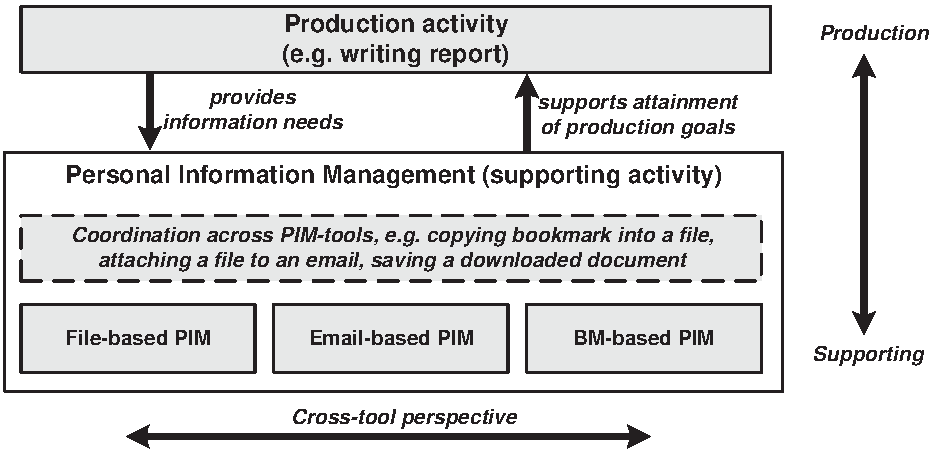
\includegraphics[height=6cm]{pictures/discussion/PIM-production-rship-pimfocus.pdf}
		% fs-fm-comparison.pdf}
	\end{center}
	\caption{Theoretical framework extended to reflect the cross-tool, supporting nature of PIM}
	\label{fig:design:PIM-production-simple}
\end{figure}


%%%%%%%%%%%%%%%%%%%%%%%%%%%%%%%%%%%%%%%%%%%%%
% MAPPING FROM PIM-TOOLS TO PRODUCTION TASKS
%%%%%%%%%%%%%%%%%%%%%%%%%%%%%%%%%%%%%%%%%%%%%
%%%%%%%%%%%%%%%%%%%%%%%%%%%%%%%%%%%%%%%%%%%%%%%%%%%%%%%%%%%%%%%%%%%%%%%%%%%%%%%%%%%%%%%%%%%%%5
% Note that not a simple mapping. Actually, many-many between PIM-tools and production tasks.
%%%%%%%%%%%%%%%%%%%%%%%%%%%%%%%%%%%%%%%%%%%%%%%%%%%%%%%%%%%%%%%%%%%%%%%%%%%%%%%%%%%%%%%%%%%%%%
% But note: not simply so, see production activities below -- have to relate to multiple strategies/multiple production activities. Some are cross-tool, some are not. However, it is not a simple mapping from PIM-tools to production activities.
% Actually, many-many between PIM-tools and production tasks.
% There is a many-many mapping between PIM-systems and production activities. % In other words, production activities vary in terms of how many PIM-tools are involved in supporting them.  
Two types of production activity can be identified in terms of the number of PIM-tools which support them:

\begin{enumerate}

\item Some production activities are \textit{tool-specific} -- they only involve PIM activity within the bounds of one PIM-tool.  A simple example of a tool-specific production activity is offered: arranging a picnic with friends. This involves the exchange of emails with friends, and their storage.  At a later time, the received messages are consulted to edit a reminder to coordinate who is bringing what food and drink.  The PIM needs for this task are email-specific.  Tool-specific production activities do not require integration support.
%%%%%%%%%%%%%%%%%%%%%%%%%%%%%%%%%%%%%%%%%%%%%%%%%%%%%%%%%%%%%%%%%
% Different PIM-tools have different \textit{raison d'etres}? 
% Core functions. This is a different slicing of activity space
%%%%%%%%%%%%%%%%%%%%%%%%%%%%%%%%%%%%%%%%%%%%%%%%%%%%%%%%%%%%%%%%%
% Email tools can be considered to be PIM tool that primarily supports the communication needs of production tasks.  Likewise, bookmark tools are a PIM-tool that primarily supports the information retrieval needs of production tasks.  Thus production activities focused on one of these aspects (e.g. book flight) may naturally be limited to one PIM-tool.

%%%%%%%%%%%%%%%%%%%%%%%%%%%%%%%%%%%%%%%%%%%%%%%%%%%%%%%%%%%%%%%%%%%%%%%%%%%%%%%
% Discuss: ONE PRODUCTION TASK/MANY PIM-tools
% Some cross-tool production tasks may be centered on particular PIM-tools.
%%%%%%%%%%%%%%%%%%%%%%%%%%%%%%%%%%%%%%%%%%%%%%%%%%%%%%%%%%%%%%%%%%%%%%%%%%%%%%%
% NB: different tools can act as gateway into a cross-tool task
%%%%%%%%%%%%%%%%%%%%%%%%%%%%%%%%%%%%%%%%%%%%%%%%%%%%%%%%%%%%%%%%%%%%%%%%%%%%%%%
% True cross-tool tasks (with primary tools?)
% Tool-dominated tasks which involved "`excusrsions"' to other tools
% Some production activities are distributed.
% \textbf{Section~\ref{discussion:cross-tool}} introduces the notion of PIM as a cross-tool activity, one that bridges multiple tools.  Some production tasks may require support from multiple PIM-tool contexts.  Provide benchmark cross-tool production tasks: Nice example. Show how it necessitates \textbf{coordination} of sub-activities and tools towards a common goal. Example cross-tool production task,e.g. more organizational needs in one tool: ISIS (may still be tool-driven). 
\item Other production activities are \textit{cross-tool} -- they involve the management of information in multiple PIM-tools.  For example, planning a holiday may involve collating websites, sending and storing emails, and creating files with possible itineraries.
%
%%%%%%%%%%%%%%%%%%%%%%%%%%%%%%%%%%
% RELATE TO INTEGRATION MECHANISMS
%%%%%%%%%%%%%%%%%%%%%%%%%%%%%%%%%%%
When production activities involve multiple PIM tools, there is the need for \textit{coordination} between those PIM-tools.  This may be as simple as transferring a bookmark from a web browser to include in an email message.  Alternatively, coordination may be more extensive, e.g. the ongoing management of emails and bookmarks relating to a long-term project. 
% Show how ONE-MANY necessitates \textbf{coordination} of sub-activities and tools towards a common goal. 
% Such production tasks that require cross-tool PIM support, may necessitate coordination of PIM activity across multiple tools.  
% Another example would be retrieving a holiday itinerary, when the user is not sure if it is stored in the file system, or as an email attachment. Other coordination examples include starting or finishing a project that involves multiple PIM tools.
%%%%%%%%%%%%%%%%%%%%%%%%%%%%%%%%%%%%%
% Discuss integration as designed-in coordination, alternative is manual coordination
% Where does integration fit in?
%%%%%%%%%%%%%%%%%%%%%%%%%%%%%%%%%%%%
% Certain production activities involve the coordination of multiple PIM-tools.  Integration mechanisms between PIM-tools can help support such coordination activities.
\textit{Integration mechanisms} can be viewed as interface functionality which support cross-tool coordinating activities, thus avoiding the need for manual coordination. By making it easier to coordinate information requirements across multiple PIM-tools, the overheads of manual coordination are lessened.
% In particular, the importance of integration between the PIM-tools involved in cross-tool production activities is noted. 
% Integration mechanisms can relieve users of some of the burden of performing coordination activities.  For example, the Windows ``Send-to'' mechanism allows bookmarks to be sent directly as email messages.

\end{enumerate}

%%%%%%%%%%%%%%%%%%%%%%%%%%%%%%%%%%%%%%%%%%%%%%%%%%%%%%%%%%%%%%%%%%%%
% \subsubsection{A final note on PIM as a supporting activity}
%%%%%%%%%%%%%%%%%%%%%%%%%%%%%%%%%%%%%%%%%%%%%%%%%%%%%%%%%%%%%%%%%%%%


% It is argued that much of the literature focuses on PIM as a production ``work'' task.  
% WHERE TO PLACE: DISCUSS INTERFERENCE WITH PRODUCTION TASKS + LIBRARIAN
This section has discussed how PIM is not a self-contained, stand-alone activity, but one that is driven by a user's production activities.  However, note that information management can itself be a production activity.  For example, consider how librarians manage information for others as one of their key job responsibilities.

% In contrast, PIM is conceptualized here as a supporting activity, one that is driven by the information needs provided by a user's production tasks\footnote{Note that some aspects of PIM may be considered as a self-contained production task by some, e.g. maintenance.}.
The relationship between PIM as a supporting activity, and a user's production activities also illustrates the distraction that PIM can cause.  At times, PIM may interfere with a user's production activities by consuming all of a user's attention.  For example, consider the situation when a user is unable to find a very important document and devotes an entire morning to finding it. In this case, PIM may displace the goals corresponding to the ``real'' production activity. \textbf{Section~\ref{discussion:uxp}} discusses the methodological implications caused by the potential of PIM to cause such distraction: do PIM designers run the risk of encouraging users to spend less time on their production activities?





%%%%%%%%%%%%%%%%%%%%%%
% LINK TO THEORY
%%%%%%%%%%%%%%%%%%%%%%
% \textit{Include links to design and theory-building}
%%%%%%%%%%%%%%%%%%%%%%%%%%%%%%%%
% LINK TO BALANCE SECTION
%%%%%%%%%%%%%%%%%%%%%%%%%%%%%%%%
% Relate to models developed in \textbf{Section~\ref{disc:study-discussion}} in terms of the ``need for balance'' (user needs to do enough PIM to support production activities, but not too much to become distracted). 
% Also relate to design ideas in \textbf{Section~\ref{disc:design-guidelines-discussion}}.
% Pros and cons of discretional supporting activity
% Potential for interference, impact on productivity on upside and downside.  Therefore need for balance.  Lead onto the next section.
%%%%%%%%%%%%%%%%%%%%%%%%%%%%%%%%%%%%%
% LINK - develop user experience
%%%%%%%%%%%%%%%%%%%%%%%%%%%%%%%%%%%%%
% Furthermore, it is these high-level activities that distract their attention from PIM.}


%%%%%%%%%%%%%%%%%%%%%%%%%%%%%%%%%%%%%%%%%%%%%%%%%%%%%%%%%%%%%%%%%%%%%%%%%%%%%%%%%%%%%%%%%%%%%%%%%%%%%%%%%%%%%%%%%
%%%%%%%%%%%%%%%%%%%%%%%%%%%%%%%%%%%%%%%%%%%%%%%%%%%%%%%%%%%%%%%%%%%%%%%%%%%%%%%%%%%%%%%%%%%%%%%%%%%%%%%%%%%%%%%%%
%%%%%%%%%%%%%%%%%%%%%%%%%%%%%%%%%%%%%%%%%%%%%%%%%%%%%%%%%%%%%%%%%%%%%%%%%%%%%%%%%%%%%%%%%%%%%%%%%%%%%%%%%%%%%%%%%
%%%%%%%%%%%%%%%%%%%%%%%%%%%%%%%%%%%%%%%%%%%%%%%%%%%%%%%%%%%%%%%%%%%%%%%%%%%%%%%%%%%%%%%%%%%%%%%%%%%%%%%%%%%%%%%%%



%%%%%%%
% FIN
%%%%%%%

%%%%%%%%%%%%%%%%%%%%%%%%%%%%
% CHAPTER 7 - DISCUSSION of THEORY: ONGOING
%%%%%%%%%%%%%%%%%%%%%%%%%%%%
%%%%%%%%%%%%%%%%%%%%%%%%%%%%%%%%%%%%%%%%%%%%%%%%%%%%%%%%%%%%%%%%%%%%%%%%%%%%%%%%%%%%%%%%%%
% Richard Boardman PhD Thesis: Improving Tool Support for Personal Information Management
%%%%%%%%%%%%%%%%%%%%%%%%%%%%%%%%%%%%%%%%%%%%%%%%%%%%%%%%%%%%%%%%%%%%%%%%%%%%%%%%%%%%%%%%%%

% \newpage
%%%%%%%%%%%%%%
% ONGOING
%%%%%%%%%%%%%%
%%%%%%%%%%%%%%%%%%%%%%%%%%%%%%%%%%%%%%%
\subsection{PIM as an Ongoing Activity}
\label{discussion:ongoing}
%%%%%%%%%%%%%%%%%%%%%%%%%%%%%%%%%%%%%%%
% The previous two sections have discussed PIM as a \textit{cross-tool} and \textit{supporting} activity in turn.
This section views PIM from a third theoretical perspective, as an \textit{ongoing} activity.
%%%%%%%%%%%%%%%%%%%%%%%%%%%%%%%%%%%%%%%%%%%%%
% PIM as continuous, background activity
%%%%%%%%%%%%%%%%%%%%%%%%%%%%%%%%%%%%%%%%%%%%%
The main study reported in \textbf{Chapter~\ref{chapter:main-study}} tracked PIM behaviour over time in terms of four PIM sub-activities: acquisition, organization, maintenance and retrieval. \textbf{Figure~\ref{fig:discussion:ongoing-model-SIMPLE}} illustrates how each of these sub-activities can be viewed on a both a short-term and long-term time-scale:

%%%%%%%%%%%%%%%%%%%%%%%%%%%%%%%%%%%%%%%%%%%%%%%%%%%%%%%%
% Break-down into parallel threads and one-off events
%%%%%%%%%%%%%%%%%%%%%%%%%%%%%%%%%%%%%%%%%%%%%%%%%%%%%%%%
% PIM is in turn made up of parallel threads corresponding to the PIM sub-activities: .
% Therefore can analyse in terms of a sequence of short-term discrete events corresponding to the acquisition, organization, maintenance and retrieval of specific items. Consider PIM as one-off local events, e.g. retrieving an item from an email collection.
% The sub-activities that make up PIM, , can all be considered to be ongoing activities, as shown in .
%%%%%%%%%%%%%%%%%%%%%%%%%%%%%%%%%%%%%%%%%%%%%%%%%%
% Model of at two levels: short-term, long-term
%%%%%%%%%%%%%%%%%%%%%%%%%%%%%%%%%%%%%%%%%%%%%%%%%%
% PIM can be considered from two perspectives, an ongoing long-term one, and from a short-term time-scale of discrete events: 
\begin{enumerate}

% PIM can also be considered to be made up of a sequence of one-off events that happen at a specific point in time.  
\item From a \textit{short-term} perspective, each sub-activity consists of a sequence of discrete events. For example, the acquisition sub-activity within a file context consists of a series of file-saving events. 
% The relative frequency of PIM sub-activities is considered. 
\textbf{Section~\ref{disc:study-discussion:growth}} noted the relative frequency of a user performing the four sub-activities. This is reflected in \textbf{Figure~\ref{fig:discussion:ongoing-model-SIMPLE}}: whilst acquisition and retrieval occur frequently, organization and maintenance are more sporadic.

\item Alternatively, from a long-term perspective, PIM can be viewed as four continuous threads of behaviour, each corresponding to the four PIM sub-activities and consisting of a sequence of discrete events.  PIM behaviour over time is therefore the combination of the four interleaved sub-activities, amounting to a continuous, background thread of activity.   In the extreme, PIM behaviour is now \textit{lifelong} since users can collect and store information over their entire lifetime~\citep{bell:02,dix:02}.  
% Each thread can be decomposed into a sequence of discrete events.

\end{enumerate}


%%%%%%%%%%%%%%%%%%%%%%%%%%%%%%%%%%%%%%
% %%%%%%%%%%%%%%%%%%%%%%%%%%%%%%%%%%%%
% FIGURE - An ongoing model of PIM
% %%%%%%%%%%%%%%%%%%%%%%%%%%%%%%%%%%%%
%%%%%%%%%%%%%%%%%%%%%%%%%%%%%%%%%%%%%%
\begin{figure}[hbtp]
	\begin{center}
		\leavevmode
		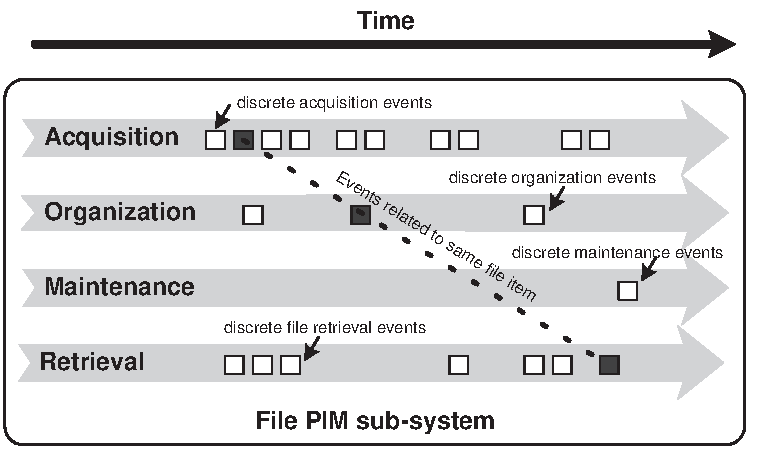
\includegraphics[height=6cm]{pictures/discussion/PIM-ongoing-model-SIMPLE.pdf}
	\end{center}
	\caption{PIM as an ongoing activity, consisting of four parallel threads corresponding to the four PIM sub-activities}
	\label{fig:discussion:ongoing-model-SIMPLE}
\end{figure}

%%%%%%%%%%%%%%%%%%%%%%%%%%%%%%
% PIM BEHAVIOUS AS A WHOLE
%%%%%%%%%%%%%%%%%%%%%%%%%%%%%%
Following from the long-term view of PIM, a number of discussion points can be raised.  
\begin{itemize}

%%%%%%%%%%%%%%%%%%%%
% STRATEGIES
%%%%%%%%%%%%%%%%%%%%
% PIM can be considered as a continuous, background thread of activity, carried out in support of a user's production tasks. Note that PIM can be considered to be distributed both over tools and over time.
\item Just as production activities may evolve over time (consider the stages of writing a report), so may the activities supporting them.  For example, \textbf{Section~\ref{main-study:results:changes}} described how PIM strategies may change over time.  The very notion of a PIM strategy suggests that behaviour is pre-planned and consistent.  However, the supporting nature of PIM means that users rarely devote time to planning and executing changes in strategy.  Instead, PIM strategies are not pre-determined, but the amalgam of many spur-of-the-moment discrete events.  For example, Participant 2 in the exploratory study reported: \textit{``I start working with something, create a new dedicated area, and then forget about it''}.  In the past, when researchers have talked about ``organizing strategies'', they are typically describing \textit{average behaviour over the long-term}
\footnote{The term \textit{average} acknowledges the multiple strategies employed by many users to manage different types of information, e.g. filing information related to some production activities but not others (see \textbf{Section~\ref{exp-study:discussion:multiple-strategies}}).}.
% As discussed in \textbf{Chapter~\ref{chapter:exploratory_study}}, users may employ different strategies }.  %  Furthermore, such low-level strategies may change over time.  
% In addition, the word ``strategy'' has the connotation that users devote time to selecting that strategy. 




% .  Whilst PIM is an ongoing thread of activity which evolves over time, information retrieval 
\item The long-term perspective allows PIM to be contrasted with information retrieval, which is typically considered to be a one-off discrete event.  In contrast, Wilson's ``human information behaviour''~\citep{wilson:00} is equivalent to the ongoing retrieval sub-activity thread, portrayed here as one aspect of PIM.  

%%%%%%%%%%%%%%%%%%%%%%%%%%%%%%%%%%%%%%%%%%%%%
% Inter-relating the sub-activities of PIM}: 
%%%%%%%%%%%%%%%%%%%%%%%%%%%%%%%%%%%%%%%%%%%%%
% \item Inter-equivalence of storage and retrieval (on-demand organization) DISCUSS: THINK: retrieval is effectively organization (enforcing a particular view of the data-set) at "query time". On-demand organization.
%%%%%%%%%%%%%%%%%%%%%%%%%%%%%%%%%%%%%%%%%%%%%%%%%%%%%%%%%%%%%%%%%%%%%%%%%%%%%%%%%%
%%%%%%%%%%%%%%%%%%%%%%%%%%%%%%%%%%%%%%
% Linking events across the threads
%%%%%%%%%%%%%%%%%%%%%%%%%%%%%%%%%%%%%%
% The long-term perspective is important as .  The acquisition of an item, may correspond to a retrieval event months later: at two different points in time.
% PIM is more continuous than information-seeking although made up of discrete events over time.  By considering PIM over time, it can be seen that events in separate threads, that occur at different times are related.  
% an example acquisition event is saving a newly-created file, which may be retrieved at a later date via a distinct retrieval event.  An example of this is indicated by the black squares in 
% Within a specific PIM sub-system, the individual acquisition events in a particular sub-activity amount to the user's total acquisition over time. 
\item The four threads in \textbf{Figure~\ref{fig:discussion:ongoing-model-SIMPLE}} are not independent -- they each represent a series of actions performed within a single collection of information.  Indeed, discrete events in two different threads may be associated by involving the same item of information.  To illustrate this point, the black squares in \textbf{Figure~\ref{fig:discussion:ongoing-model-SIMPLE}} indicate the association between the acquisition, storage and later retrieval of a particular item.  

The nature of one sub-activity can influence how users perform other sub-activities. For example, the rate at which users acquire items, influences their choice of organization, maintenance and retrieval strategies.
% In turn, if users organize items within folders, this leads to the need to organize those folders as well as the items they contain.
Also, organization and maintenance have a strong influence on retrieval.  Several participants commented that maintaining their collections (e.g. tidying, deleting items) could make it harder to find items.  % It is noted that Barreau's division of PIM into four distinct sub-activities may obscure such inter-relationships. %
% \begin{itemize}
%%%%%%%%%%%%%%%%%%%%%%%%%%%%%%%%%%%%%%%%%%%%%%%
% The sub-activities influence one another
% \item Several users mentioned downside of org for search/sort (I try to minimise structure as I find by sorting on date and sender metadata to get a flexible view)
% \item Cost-benefit trade-off in storage/retrieval. When to invest time. Many users perceive that org leads to faster retrieval.  But also that no org is better.
%%%%%%%%%%%%%%%%%%%%%%%%%%%%%%%%%%%%%%%%%%%%%%%
% * Acquisition - leads to clutter and need to organize. Over time, shift from item-clutter to folder-clutter
%%%%%%%%%%%%%%%%%%%%%%%%%%%%%%%%%%%%%%%%%%%%%%%%%%%%%%%%%%%%%%%%%	
% The sub-activities overlap
% Acquisition (allocation of value) as ``not deleting'' (email)
% Acquisition as implicit storage/organization (implicit metadata). Explicit organization as extra
%%%%%%%%%%%%%%%%%%%%%%%%%%%%%%%%%%%%%%%%%%%%%%%%%%%%%%%%%%%%%%%%%
% \item The sub-activities often overlap. For example, in email deciding what new messages to delete from the inbox (inbox maintenance), can be viewed as a form of acquisition (deciding what to add to the collection).
%%%%%%%%%%%%%%%%%%%%%%%%%%%%%%%%%%%%%%%%%%%
% Need better definition of acquisition
%%%%%%%%%%%%%%%%%%%%%%%%%%%%%%%%%%%%%%%%%%%
% \item Compare acquisition of new item, and re-saving edited version of one that already exists
% * Acquisition - too easy to acquire
% \end{itemize}

\end{itemize}




%%%%%%%%%%%%%%%%%%%%%%%%%%%%%%%%%%%%%%%%%%%%%%%%%%%%%%%%%%%%%%%%%%%%%%%%%%%%%%%%%
% THINK: relationship with information retrieval here rather than in Chapter 2}
%%%%%%%%%%%%%%%%%%%%%%%%%%%%%%%%%%%%%%%%%%%%%%%%%%%%%%%%%%%%%%%%%%%%%%%%%%%%%%%%%%


%%%%%%%%%%%%%%%%%%%%%%%%%%%%%%%%%%%%%%%%%%%%%%%%%%%%%%%
\subsubsection{Extending the Theoretical Framework}
%%%%%%%%%%%%%%%%%%%%%%%%%%%%%%%%%%%%%%%%%%%%%%%%%%%%%%%

\textbf{Figure~\ref{fig:discussion:ongoing-model}} shows the theoretical framework extended to accommodate all three perspectives discussed in this section: (1) \textit{cross-tool}, (2) \textit{supporting}, and (3) \textit{ongoing}.  % It can be argued that previous work in this area has not focused on these aspects, so each highlights promising routes for future work in terms of theoretical development or empirical investigation. 


% Now the theoretical framework shown in \textbf{Figure~\ref{fig:design:PIM-production-simple}} is extended to reflect the ongoing perspective on PIM outlined above.
% LINK TO CROSS-TOOL DISCUSSION: added need for cross-tool coordination as PIM is distributed over time AND across too
% The combined framework is shown in \textbf{Figure~\ref{fig:discussion:ongoing-model}}. 
The figure shows two example production activities (A and B) and the associated PIM activity.  The squares and triangles refer to PIM events relating to production activity A and B, respectively.   PIM is also shown to be distributed \textit{across tools}, and \textit{over time} (horizontal axis).    The figure reflects variations in the frequency of PIM events between tools.  Due to the discretionary nature of PIM, events in the parallel threads, relating to various production activities, may be interleaved arbitrarily.

%%%%%%%%%%%%%%%%%%%%%%%%%%%%%%%%%%%%%%
% %%%%%%%%%%%%%%%%%%%%%%%%%%%%%%%%%%%%
% FIGURE - An ongoing model of PIM
% %%%%%%%%%%%%%%%%%%%%%%%%%%%%%%%%%%%%
%%%%%%%%%%%%%%%%%%%%%%%%%%%%%%%%%%%%%%
\begin{figure}[hbtp]
	\begin{center}
		\leavevmode
		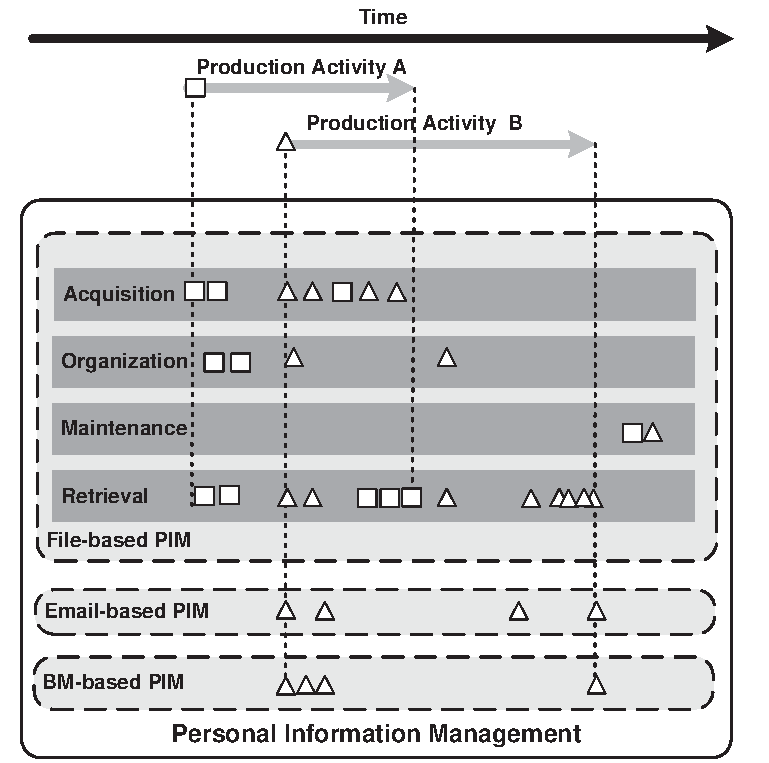
\includegraphics[height=10cm]{pictures/discussion/PIM-ongoing-model.pdf}
	\end{center}
	\caption{Theoretical framework extended to reflect the cross-tool, supporting, and ongoing nature of PIM}
	\label{fig:discussion:ongoing-model}
\end{figure}

%%%%%%%%%%%%%%%%%%%%%%%%%%
% LINK TO OTHER SECTIONS
%%%%%%%%%%%%%%%%%%%%%%%%%%
%The next section considers how PIM behaviour may evolve over time.  Such insights may shed light on the uptake of new tools by users.
% Methodological implications for evaluating PIM-tools are considered in \textbf{Section~\ref{discussion:methodological-discussion}}.


%%%%%%%%%%%%%%%%%%%%%%%%%%%%%%%%%%%%%%%%%%%%%%%%%%%%%%%%%%%%%%%%%%%%%%%%%%%%%%%%%%%%%%%%%%%%%%%%%%%%%%%%%%%%%%%%%
%%%%%%%%%%%%%%%%%%%%%%%%%%%%%%%%%%%%%%%%%%%%%%%%%%%%%%%%%%%%%%%%%%%%%%%%%%%%%%%%%%%%%%%%%%%%%%%%%%%%%%%%%%%%%%%%%
%%%%%%%%%%%%%%%%%%%%%%%%%%%%%%%%%%%%%%%%%%%%%%%%%%%%%%%%%%%%%%%%%%%%%%%%%%%%%%%%%%%%%%%%%%%%%%%%%%%%%%%%%%%%%%%%%
%%%%%%%%%%%%%%%%%%%%%%%%%%%%%%%%%%%%%%%%%%%%%%%%%%%%%%%%%%%%%%%%%%%%%%%%%%%%%%%%%%%%%%%%%%%%%%%%%%%%%%%%%%%%%%%%%


%%%%%%%%%%%%%%%%%%%%%%%%%
\subsection{Towards a Theory of PIM}
\label{discussion:towards-theory}
%%%%%%%%%%%%%%%%%%%%%%%%%

%%%%%%%%%%%%%%%%%%%%%%%%%%%%%%%
% Talking about INFORMATION
%%%%%%%%%%%%%%%%%%%%%%%%%%%%%%%
The framework in \textbf{Figure~\ref{fig:discussion:ongoing-model}} illustrates three important aspects of PIM that have emerged over the course of this research programme.  Note that the framework is not intended to represent a complete model of PIM.  Instead, it is presented to illustrate three areas that must be accommodated in future theoretical work in this area.  The framework also highlights the analytical complexity of PIM as a HCI phenomenon.  One way to deal with such complexity, may be to develop an inter-linked set of theories, rather than a monolithic one~\citep{barnard:00}.

There are also many other areas in which the theoretical basis of PIM could be improved.  One other area suggested by \citet{Whittaker-rta:00} is to improve the \textit{descriptive vocabulary} for talking about personal information.  The author echoes this call.  This research points at one fundamental area in need of attention -- that is the need for a richer vocabulary to describe items of personal information beyond \textit{technological format}, and \textit{lifetime of use}~\citep{bn:95}. For example, \textbf{Chapter~\ref{chapter:exploratory_study}} advocated that the term ``archived'' is misleading, since most users do not archive explicitly.  Two alternative sets of terms are suggested:
\begin{enumerate}
	\item \textit{Information usefulness} -- \textit{active} (relating to current production activities, including ephemeral and working items), \textit{dormant} (inactive, potentially useful), \textit{not useful} (should be deleted), and \textit{un-assessed} (e.g. new emails).
	\item \textit{Information ownership} -- \textit{mine} (including self-created files, and items that have been assessed as having value, e.g. filed email), and \textit{``not-mine''} (e.g. much of the email inbox, and information on the internet).
\end{enumerate}

The subsequent sections of this discussion chapter draw on the theoretical framework developed over \textbf{Sections~\ref{discussion:cross-tool}} to \textbf{\ref{discussion:ongoing}}. Firstly, \textbf{Section~\ref{discussion:design-guidelines-discussion}} revisits the WM evaluation in lieu of the discussion of PIM as a supporting activity.  A number of design implications are discussed, focusing on improving integration between PIM-tools.  % Then, \textbf{Section~\ref{discussion:methodological-discussion}} considers methodological implications that can be drawn from the three aspects of PIM discussed above.

%%%%%%%%%%%%%%%%%%%%%%%%%%%%%%%%%%%%%%%%%%%%%%%%%%%%%%%%%%%%%%%%%%%%%%%%%%%%%%%%%%%%%%%%%%%%%%%%%%%%%%%%%%%%%%%%%
%%%%%%%%%%%%%%%%%%%%%%%%%%%%%%%%%%%%%%%%%%%%%%%%%%%%%%%%%%%%%%%%%%%%%%%%%%%%%%%%%%%%%%%%%%%%%%%%%%%%%%%%%%%%%%%%%
%%%%%%%%%%%%%%%%%%%%%%%%%%%%%%%%%%%%%%%%%%%%%%%%%%%%%%%%%%%%%%%%%%%%%%%%%%%%%%%%%%%%%%%%%%%%%%%%%%%%%%%%%%%%%%%%%
%%%%%%%%%%%%%%%%%%%%%%%%%%%%%%%%%%%%%%%%%%%%%%%%%%%%%%%%%%%%%%%%%%%%%%%%%%%%%%%%%%%%%%%%%%%%%%%%%%%%%%%%%%%%%%%%%

%%%%%%%%%%%%%%%%%%%%%%%%%%%%%
% END: THEORETICAL FRAMEWORK
%%%%%%%%%%%%%%%%%%%%%%%%%%%%%






%%%%%%%%%%%%%%%%%%%%%%%%%%%%
% CHAPTER 7 - DISCUSSION OF DESIGN IMPLICATIONS
%%%%%%%%%%%%%%%%%%%%%%%%%%%%
%%%%%%%%%%%%%%%%%%%%%%%%%%%%%%%%%%%%%%%%%%%%%%%%%%%%%%%%%%%%%%%%%%%%%%%%%%%%%%%%%%%%%%%%%%
% Richard Boardman PhD Thesis: Improving Tool Support for Personal Information Management
%%%%%%%%%%%%%%%%%%%%%%%%%%%%%%%%%%%%%%%%%%%%%%%%%%%%%%%%%%%%%%%%%%%%%%%%%%%%%%%%%%%%%%%%%%
%%%%%%%%%%%%%%%%%%%%%%%%%%%%%%%%%%%%%%%%%%%%%%%%%%%%%%%%%%%%%%%%%%%%%%%%%%%%%%%%%%%%%%%%%%
% NATBIB NOTES
%%%%%%%%%%%%%%%%%%%
%\citet{jon90}                ->    Jones et al. (1990) 
%   \citet[chap.~2]{jon90}       ->    Jones et al. (1990, chap. 2)
%   \citep{jon90}                ->    (Jones et al., 1990) 
%   \citep[chap.~2]{jon90}       ->    (Jones et al., 1990, chap. 2) 
%%%%%%%%%%%%%%%%%%%%%%%%%%%%%%%%%%%%%%%%%%%%%%%%%%%%%%%%%%%%%%%%%%%%%%%%%%%%%%%%%%%%%%%%%%

\newpage
%%%%%%%%%%%%%%%%%%%%%%%%%%%%%%%%%%%%%%%%%%%%%%%%%%%%%%%%%%%%%%%%
\section{The Design of PIM-Integration Mechanisms}
\label{discussion:design-guidelines-discussion}
%%%%%%%%%%%%%%%%%%%%%%%%%%%%%%%%%%%%%%%%%%%%%%%%%%%%%%%%%%%%%%%%
% Consider both PIM-general and PIM-integration (FOCUS).
% A focus is taken on efforts to improve integration between PIM-tools, but general implications for all PIM design is also considered.  Firstly, \textbf{Section~\ref{disc:design-guidelines-discussion-pim-integration}} focuses on efforts to improve PIM-integration.  Then \textbf{Section~\ref{disc:design-guidelines-discussion-pim-general}} discusses implications for PIM design in general, including the design of specific PIM-tools.
%%%%%%%%%%%%%%%%%%%%%%%%%%%%%%%%%%%%%%%%%%%%%%%%%%%%%%%%%%%%%%%%
% What experiences can be generalized beyond the specifics of WM for the design of PIM systems in general. What do the results mean for design of future PIM systems/OS developers?
%%%%%%%%%%%%%%%%%%%%%%%%%%%%%%%%%%%%%%%%%%%%%%%%%%%%%%%%%%%%%%%%

%%%%%%%%%%%%%%%%%%%%%%%%%%%%%%%%%%%%%%%%%%%%%%%%%%%%%%%%
% PREVIOUSLY: INTEGRATION SEEN AS A GOOD THING
%%%%%%%%%%%%%%%%%%%%%%%%%%%%%%%%%%%%%%%%%%%%%%%%%%%%%%%%
Integration between PIM-tools has been repeatedly put forward as a worthy design aim, e.g.~\citep{Bellotti:03,Bergman:03,Kaptelinin:03}.  However, \textbf{Chapter~\ref{chapter:review}} noted that most of the research prototypes that have been developed have been founded on designer intuition rather than on a systematic \textit{cross-tool} investigation of user needs.  Furthermore, few evaluations of PIM-integration mechanisms have been published.
% (certainly not published work) 
%%%%%%%%%%%%%%%%%%%%%%%%%%%
% RECAP C/T WORK PERFORMED
%%%%%%%%%%%%%%%%%%%%%%%%%%%
A key aim of this research was to systematically investigate the potential to integrate PIM-tools.  % \textbf{Chapter~\ref{chapter:exploratory_study}} reported a cross-tool study which compared the nature of PIM across PIM-tools to identify routes for integration.  \textbf{Chapter~\ref{chapter:design}} proposed a new integration mechanism based on one route, WorkspaceMirror (WM), which was then evaluated in \textbf{Chapter~\ref{chapter:main-study}}.
%%%%%%%%%%%%%%%%%%%%%%%
% INTRO THIS SECTION
%%%%%%%%%%%%%%%%%%%%%%%
%\textbf{Section~\ref{discussion:theoretical-framework}} discussed the cross-tool, supporting, and ongoing nature of PIM.  This section draws on that discussion to discuss the findings from the evaluation of WM, and consider implications for PIM integration more generally. % consider implications for the design and evaluation of PIM-tools.  Findings are drawn together and discussed from throughout the thesis, including empirical findings from the exploratory study in \textbf{Chapter~\ref{chapter:exploratory_study}}, and the longitudinal evaluation of WorkspaceMirror in \textbf{Chapter~\ref{chapter:main-study}}.
This section discusses implications for the design of more coherent, integrated PIM technologies based on the experience gained in this research.  % Firstly, the results of the WM evaluation are considered in lieu of the discussion in \textbf{Section~\ref{discussion:theoretical-framework}}.



%%%%%%%%%%%%%%%%%%%%%%%%%%%%%%%%%%%%%%%%%%%%%%%%%%%%%%%%%%%%%%%%%%%%%%%%%%%%%%%%%%%%%%%%%%%%%%%%%%%%%%%%%%%%%%%%%
%%%%%%%%%%%%%%%%%%%%%%%%%%%%%%%%%%%%%%%%%%%%%%%%%%%%%%%%%%%%%%%%%%%%%%%%%%%%%%%%%%%%%%%%%%%%%%%%%%%%%%%%%%%%%%%%%
%%%%%%%%%%%%%%%%%%%%%%%%%%%%%%%%%%%%%%%%%%%%%%%%%%%%%%%%%%%%%%%%%%%%%%%%%%%%%%%%%%%%%%%%%%%%%%%%%%%%%%%%%%%%%%%%%
%%%%%%%%%%%%%%%%%%%%%%%%%%%%%%%%%%%%%%%%%%%%%%%%%%%%%%%%%%%%%%%%%%%%%%%%%%%%%%%%%%%%%%%%%%%%%%%%%%%%%%%%%%%%%%%%%

%%%%%%%%%%%%%%%%%%%%%%%%%%%%%%%%%%%%%%%%%%%%%%%%%%%%%%%
\subsection{Revisiting the WM Evaluation}
\label{disc:design-guidelines-discussion-pim-integration}
%%%%%%%%%%%%%%%%%%%%%%%%%%%%%%%%%%%%%%%%%%%%%%%%%%%%%%%

%%%%%%%%%%%%%%%%%%%%%%%%%%%%%%%%%%
% THEORETICAL PERSPECTIVE ON WM
%%%%%%%%%%%%%%%%%%%%%%%%%%%%%%%%%%
% Extend idea of artefacts that can be designed to features that bridge across multiple tools.
% This section, proposes a new theoretical concept, that of a 
\textbf{Chapter~\ref{chapter:design}} described the design and implementation of a novel PIM-integration mechanism, WorkspaceMirror (WM), which allows the user to share folder structures between the file, email and bookmark collections via \textit{folder-mirroring}. 
%%%%%%%%%%%%%%%%%%%%%%%%%%
% Sum evaluation of WM
% Talk about the trade-off
%%%%%%%%%%%%%%%%%%%%%%%%%%
% Pros of WM: thus easier coordination in terms of organizing, more consistent mental models for retrieval)
WM was evaluated to explore the potential to share folder structures across PIM-tools. 

\textbf{Section~\ref{main-study:discussion:evaluation}} identified a trade-off between \textit{organizational consistency} and \textit{organizational flexibility}, resulting from usage of WM:

\begin{itemize}

\item On one hand, folder-mirroring allows the user to improve the consistency of organizational structures in different collections of information.  Several participants welcomed this consistency and indicated that it made retrieval more straightforward.

\item On the other hand, an increase in consistency reduces the user's flexibility to organize different types of information in different ways.  Participants stated that they required some flexibility so they could have different folder structures in different tools, as organizational requirements varied across them.  However, feedback indicated that top-level folders (typically based on their roles and projects) were often suitable for mirroring.  

\end{itemize}

%%%%%%%%%%%%%%%%%%%%%%%%
% Link to next section
%%%%%%%%%%%%%%%%%%%%%%%%
The next section offers a theoretical explanation to explain the need for organizational flexibility: \textit{why are some folders useful in multiple tool contexts, but others are not?}  The discussion employs the concepts of production and supporting activities from \textbf{Section~\ref{discussion:supporting}}. 






%%%%%%%%%%%%%%%%%%%%%%%%%%%%%%%%%%%%%%%%%%%%%%%%%%%%%%%%%%%%%%%%%%%%%%%%%%%%%%%%%%%%%%%%%%%%%%%%%%%%%%%%%%%%%%%%%
%%%%%%%%%%%%%%%%%%%%%%%%%%%%%%%%%%%%%%%%%%%%%%%%%%%%%%%%%%%%%%%%%%%%%%%%%%%%%%%%%%%%%%%%%%%%%%%%%%%%%%%%%%%%%%%%%
%%%%%%%%%%%%%%%%%%%%%%%%%%%%%%%%%%%%%%%%%%%%%%%%%%%%%%%%%%%%%%%%%%%%%%%%%%%%%%%%%%%%%%%%%%%%%%%%%%%%%%%%%%%%%%%%%
%%%%%%%%%%%%%%%%%%%%%%%%%%%%%%%%%%%%%%%%%%%%%%%%%%%%%%%%%%%%%%%%%%%%%%%%%%%%%%%%%%%%%%%%%%%%%%%%%%%%%%%%%%%%%%%%%

%%%%%%%%%%%%%%%%%%%%%%%%%%%%%%%%%%%%%%%%%%%%%%%%
\subsection{When is Folder-mirroring Appropriate?}
%%%%%%%%%%%%%%%%%%%%%%%%%%%%%%%%%%%%%%%%%%%%%%%%

\textit{Production activities} are a user's high-level activities, those which provide the information needs that drive their PIM activity.  Here, it is proposed that a user's production activities are a key influencing factor in the creation of new folders\footnote{The author notes that there may be other factors influencing the creation of folders, e.g. whether the user believes organization to be important.}.  For instance, when a user starts a new production activity that he or she predicts will involve the management of associated information, he or she may create a new folder. Alternatively, the user may create the folder some time after starting the production activity.
%%%%%%%%%%%%%%%%%%%%%%%%
% TS and CT ACTIVITIES
%%%%%%%%%%%%%%%%%%%%%%%%
% are \textit{tool-specific} in terms of their organizational requirements, whilst others are \textit{cross-tool} -- they involve the management of multiple types of information.
\textbf{Section~\ref{discussion:supporting}} also introduced the notion of \textit{tool-specific} and \textit{cross-tool} production activities.  Tool-specific production activities only involve one PIM-tool, whilst cross-tool production activities are supported by multiple PIM-tools.  The appropriateness of folder-mirroring for each type of production activities is discussed as follows:

\begin{itemize}

%%%%%%%%%%%%%%%%%%%%%%%%%%%%%%%
% BUT TOOL-SPECIFIC MAY NOT
%%%%%%%%%%%%%%%%%%%%%%%%%%%%%%%
% TOOL-SPECIFIC PROD: Many production activities are tool-specific in terms of PIM support and may be negatively impacted by folder-mirroring.  Idea of integration as causing interference, setting up connections with other activities when they are not necessary.  Use as explanation of when/why/where integration sometimes works and when it does not.	
\item \textit{Tool-specific production activities} -- Folder-mirroring is likely to be inappropriate in cases whereby an information need is tool-specific, i.e. when it corresponds to a tool-specific production activity.  Only users who place a high value on organizational consistency are likely to find folder mirroring useful in this context. For most users, mirroring may be seen to result in the creation of ``spurious folders'' in tool contexts where they are not relevant.  This may in turn lead to clutter and a sense of untidiness, causing negative user experience and retrieval difficulties.
% PROBS WITH WM: Firstly, there is the potential for spurious folders, folders that are useful in one tool context but not another.   Users do not need the same folder in all tools.  Unwanted folders may be seen to interfere with a user's control of their information space by causing clutter.
Such side-effects may be distributed in time relative to the folder creation event, e.g. the interference caused by spurious folders may not be clear until retrieval time.  % Also, different tools often require different levels of organizational granularity.  OTHER PROBLEMS: Secondly there is also the interrupting dialog boxes.



%%%%%%%%%%%%%%%%%%%%%%%%%%%
% CROSS-TOOL MAY BENEFIT
%%%%%%%%%%%%%%%%%%%%%%%%%%%
% Other production activities are cross-tool and can benefit from folder-mirroring. 
%%%%%%%%%%%%%%%%%%%%%%%%%%%%%%%%%%%%%%%%%%%%%
% Mismapping between tools and activities
%%%%%%%%%%%%%%%%%%%%%%%%%%%%%%%%%%%%%%%%%%%%%
% Therefore there has been a mis-mapping between PIM-tools and the cross-tool nature of PIM.
% Function of application basis of today's OSs.  
%Our work is based on this cross-tool perspective, and aims to provide more coherent, integrated support for PIM. We first discuss the findings from a cross-tool study of users' PIM practices.
%\begin{itemize}
%	\item Pros/cons of integration
%\end{itemize}
% ARGUE POTENTIAL FOR INTEGRATION: Problems with current tools.  Resultant mismatch between workspace-wide activities and tool-centric support. i.e. support for distributed tasks is compartmentalized. Relate to coordination.  Overhead on the user
\item \textit{Cross-tool production activities} -- Folder-mirroring is most appropriate in those cases where a new folder is driven by a cross-tool information need.  The observation of folder overlap in \textbf{Chapter~\ref{chapter:exploratory_study}} provided evidence of cross-tool information needs.  In these cases, folder-mirroring avoids the user having to create a folder separately in three different tool contexts.  In this way, folder-mirroring may help the user in coordinating their PIM requirements across all three tools.

%%%%%%%%%%%%%%%%%%%%%%%%%%%%%%%%%%%%%
% IS F-M ALWAYS APPROPRIATE FOR C/T
% PRODUCTION ACTIVITIES?
%%%%%%%%%%%%%%%%%%%%%%%%%%%%%%%%%%%%%
% Here a focus is taken on the organizational requirements from a particular production activity.  Thus 
However, folder-mirroring may not be appropriate for all cross-tool production activities.
%%%%%%%%%%%%%%%%%%%%%%%%%%%%%%%%%%%%%%%%%%%%%%%%%%%%%%%%%%%%%%%%%
% DIFFERENT FOLDERS FOR THE SAME PROJECT IN DIFFERENT TOOSL
%%%%%%%%%%%%%%%%%%%%%%%%%%%%%%%%%%%%%%%%%%%%%%%%%%%%%%%%%%%%%%%%%
Firstly, the user may wish to store information related to a particular cross-tool production activity in folders with different names in different tool contexts.  For example, folders corresponding to a software project may be named after the project code in email, but after the project manager in the file system. % \textit{Indeed one can imagine a particular concept being used to refer to different information needs in different tool contexts.}
%%%%%%%%%%%%%%%%%%%%%%%%%%%%%%%%%%%%%%%%%%%%%%%%%%%%%%%
% different organizational requirements in each tool
%%%%%%%%%%%%%%%%%%%%%%%%%%%%%%%%%%%%%%%%%%%%%%%%%%%%%%%
Secondly, users may have varying organizational requirements across different tool contexts.  Files are generally much more richly and deeply structured than emails or bookmarks.  This explains the bias towards mirroring top-level folders: lower-level folders as developed most often in the file system are not useful in the other contexts.

% \item ADD: multiple projects to the same folder

These examples illustrate that it should not be assumed that a cross-tool production activity will always require mirroring.  However, the author argues that the conceptualization of cross-tool production activities is useful as an indication of where folder-mirroring is likely to be appropriate.

\end{itemize}

% \textit{Note that the above examples make the assumption that production activities require the organization of information.}


%%%%%%%%%%%%%%%%%%%%%%%%%%%%%%%%%%%%%%%%%%%%%%%%%%%%%%%%%%%%%%%%%%%%%%%%%%%%%%%%%%%%%%%%%%%%%%%%%%%%%%%%%%%%%%%%%
%%%%%%%%%%%%%%%%%%%%%%%%%%%%%%%%%%%%%%%%%%%%%%%%%%%%%%%%%%%%%%%%%%%%%%%%%%%%%%%%%%%%%%%%%%%%%%%%%%%%%%%%%%%%%%%%%
%%%%%%%%%%%%%%%%%%%%%%%%%%%%%%%%%%%%%%%%%%%%%%%%%%%%%%%%%%%%%%%%%%%%%%%%%%%%%%%%%%%%%%%%%%%%%%%%%%%%%%%%%%%%%%%%%
%%%%%%%%%%%%%%%%%%%%%%%%%%%%%%%%%%%%%%%%%%%%%%%%%%%%%%%%%%%%%%%%%%%%%%%%%%%%%%%%%%%%%%%%%%%%%%%%%%%%%%%%%%%%%%%%%

%%%%%%%%%%%%%%%%%%%%%%%%%%%%%%%%%%%%%%%%%%%%%%%%%%%%%%%%%%%%%%
% \subsubsection{Weighing up the pros and cons of integration}
%%%%%%%%%%%%%%%%%%%%%%%%%%%%%%%%%%%%%%%%%%%%%%%%%%%%%%%%%%%%%%

%%%%%%%%%%%%%%%%%%%%%%%%%%%%%%%%%%%%%%%%%%%%%%%%%%%%%%%%%%%%%%%%%%%%%%%%%%%%%%%%
% Thus need for prompting -- user has to decide whether mirroring is necessary. 
%%%%%%%%%%%%%%%%%%%%%%%%%%%%%%%%%%%%%%%%%%%%%%%%%%%%%%%%%%%%%%%%%%%%%%%%%%%%%%%%
% do the overall strengths of the design outweigh its weaknesses.  
The above discussion highlights some of the strengths and weaknesses of the folder mirroring technique, in terms of the benefits offered for different kinds of production activity.  The question to be investigated in evaluation is: does the \textit{consistency} introduced by folder-mirroring outweigh the impact on the \textit{flexibility} to have different folder structures in different tools?  The evaluation results suggest that response to this question is idiosyncratic: some users value consistency more, whilst others value flexibility higher.  Since users vary in their need for such a mechanism, the author concludes that such functionality should be optional and configurable\footnote{The author observes that the WM design has other strengths and weaknesses which must be taken into account during evaluation beyond the trade-off between flexibility and consistency.  For instance, two other weaknesses include: (1) the additional cognitive load of making the decision on whether to mirror, and (2) the effect of the prompting interruption.  In evaluation, the net strengths of the design must be weighed against the net weaknesses.}.  



%%%%%%%%%%%%%%%%%%
% IDIOSYNCRATIC
%%%%%%%%%%%%%%%%%%
%%%%%%%%%%%%%%%%%%%%%%%%%%%%%%%%%%%%%%%%%%%%%%%%%%%%%%%
% lessons for PIM integration based on organization
%%%%%%%%%%%%%%%%%%%%%%%%%%%%%%%%%%%%%%%%%%%%%%%%%%%%%%%
% The question is can this cause interference for tool-specific production tasks, or other cases where folder-mirroring is inappropriate? 
% \textit{Likewise unifying unfiled email and files. 
% but hopefully illustrates key lessons for others: flexibility is of importance and implicitly promoted when multiple specialized tools are present.  The increase in consistency offered by some forms of PIM-integration may impact flexibility.

% How did users respond? Users seemed to differ. Some yes. Some no.  Idiosyncratic. Fall on different sides of the fence.  Therefore good that its an option. Most promising for top-level folders.
WM represents a modest step towards the more advanced integration promised by new operating system designs such as \textit{MS-Longhorn}~\citep{winfs:03}, and research prototypes such as \textit{Haystack}~\citep{haystack:99}.  Whilst WM offers integration in terms of mirroring folder structures between PIM-tools, these more ambitious systems facilitate the management of different types of information within a common organizational mechanism.  With WM, users still have to manage distinct collections of information separately. 

Feedback from the evaluation of WM included several recommendations for improving its design as a specific PIM-integration mechanism (see \textbf{Section~\ref{main-study:results:themes-design-recs}}).  However, the evaluation also offers two lessons for the wider design genre of PIM-integration:
\begin{enumerate}

\item \textit{The consistency/flexibility trade-off} -- The WM evaluation illustrates that an increase in organizational consistency across different types of information may impact organizational flexibility.  The author believes that an awareness of this trade-off will be useful for the designers of integration mechanisms that incorporate organizing functionality.

\item \textit{The pros and cons of integration} -- Some cross-tool designs will not provide integration in terms of organizing functionality as WM does.  However, the WM case-study illustrates another more general implication for the wider design genre: that for any integration design, there will be a cost-benefit trade-off which must be carefully considered when evaluating the design. 

\end{enumerate}


%%%%%%%%%%%%%%%%%%%%%%%%%%%%%%%%%%
\subsection{The Pros and Cons of Integration}
%%%%%%%%%%%%%%%%%%%%%%%%%%%%%%%%%%

%%%%%%%%%%%%%%%%%%%%%%%%%%%%%%%%%%%%%%%%%%%%%%%
% Generalize to pros and cons of integration
%%%%%%%%%%%%%%%%%%%%%%%%%%%%%%%%%%%%%%%%%%%%%%%
The second implication listed above, that an integration design may have pros and cons, may appear obvious to the reader.  However, the author observes that in many cases, only the positive aspects of integration are considered, e.g. in marketing literature.  The author is not aware of any in-depth investigations of the possible downsides of integration.  

The implications of any design may be difficult for designers to predict before it is evaluated.  This is particularly the case for integration mechanisms, where costs and benefits may be distributed both across tools and over time.  In other words, benefits in tool A at time X, may be offset by costs in tool B at time Y.  The attachment mechanism is employed to illustrate this point.  This functionality allow non-native information to be communicated via email without the need for re-formatting, and was the most-common form of integration mentioned by participants in the main study.  % The key benefit of the attachment mechanism is to 
% However, the attachment mechanism has positive and negative consequences from a cross-tool perspective.  The mechanism allow integration between files and emails in terms of attaching files to messages to send to other users
However, the attachment mechanism has a side-effect when viewed from a cross-tool perspective: it enables the storage of files in multiple locations. This distribution of files across multiple tools, so-called \textit{compartmentalization}~\citep{Bellotti:00}, may cause retrieval difficulties if a user is not sure of the location of a required file.  This negative issue is a side-effect of designer's well-intentioned aims to improve integration between email and other tools.  The benefits of allowing the attachment of files to emails results in the negative consequence of the file collection being compartmentalized.

%%%%%%%%%%%%%%%%%%%%%%%%%%%%%%%%%%%%%%%%%%%%%%%%%%%%%%%%%%%%%%%%%%%%%%%%%%%%%%%%%%%%%%%%%%%%%%%%%%%%%%%%%%%%%%%%%
%%%%%%%%%%%%%%%%%%%%%%%%%%%%%%%%%%%%%%%%%%%%%%%%%%%%%%%%%%%%%%%%%%%%%%%%%%%%%%%%%%%%%%%%%%%%%%%%%%%%%%%%%%%%%%%%%
%%%%%%%%%%%%%%%%%%%%%%%%%%%%%%%%%%%%%%%%%%%%%%%%%%%%%%%%%%%%%%%%%%%%%%%%%%%%%%%%%%%%%%%%%%%%%%%%%%%%%%%%%%%%%%%%%
%%%%%%%%%%%%%%%%%%%%%%%%%%%%%%%%%%%%%%%%%%%%%%%%%%%%%%%%%%%%%%%%%%%%%%%%%%%%%%%%%%%%%%%%%%%%%%%%%%%%%%%%%%%%%%%%%

% A key reason for the mistaken belief of the contrary is a lack of understanding regarding the nature of PIM, something which the work reported in this thesis has attempted to overcome.    -- \textit{that integration was a good thing, surely there is no need to manage different types of information in different ways?}
%%%%%%%%%%%%%%%%%%%%%%%%%%%%%%%%%%%%%%%
% Limitations of integration view
%%%%%%%%%%%%%%%%%%%%%%%%%%%%%%%%%%%%%%%
% Limitations to potential to integrate/unify. These study results suggest counter-argument to unification - benefits of applications. Along lines of Norman's Information Appliance view - simple and specialized.  \textit{THINK: should I claim this as aim of study, or just the result of a measured investigation?}. ADD USER COMMENTS
% \textit{SUPPORTED BY EMPIRICAL DATA}:
Another negative consequence of some integration designs may be increased complexity.  \textbf{Section~\ref{review:embedding}} observed the increase in complexity caused by \textit{embedding} support for managing non-native technological formats within a PIM-tool.  In addition, one participant in the main study commented that application suites which contain multiple PIM-tools, such as Netscape Communicator or Outlook, were ``too integrated''. % ADD MORE USER COMMENTS

%%%%%%%%%%%%%%%%%%%%%%%%%%%%%%%%%%%%%%%%%%%%%%%%%%%%%%%%%%%%%%%%%%%%%%
% HOWEVER there is potential for too much in the way of integration
%%%%%%%%%%%%%%%%%%%%%%%%%%%%%%%%%%%%%%%%%%%%%%%%%%%%%%%%%%%%%%%%%%%%%%
% Leading into potential for interference between collections if inappropriate integration. 
%%%%%%%%%%%%%%%%%%%%%%%%%%%
% Compartmentalization
%%%%%%%%%%%%%%%%%%%%%%%%%%%
% Tools are ``focused'' on one info type.  THerefore user goes there to find info of that type.
%%%%%%%%%%%%%%%%%%%%%%%%%%%
% Some problems caused by haphazard integration, e.g. compartmentalization.  The ability to manage a particular technological format in different collections, causes benefits and problems.  Danger of a piecemeal approach. Consider compartmentalization in abstract terms as a set of constraints on the user. 
% Need for integration, but can be bad.  However, integration can have unintended effects, for example:
% Although each tool is focused on information of a particular technological format (or range of formats in the case of the file system), some are able to handle information of other formats. For example, users are able to manage files as email attachments within many email tools. 
The examples described in this section illustrate that integration may offer benefits whilst at the same time causing problems for users. 
%%%%%%%%%%%%%%%%%%%%%%%%%%%%%%%%%%%%%%%%%%%%%%%%%%%%%%%%%%%%%%%%%%%%%%%%%%%%%%%%%%%%%%
% KEY DISCUSSION POINT: Integration is not all rosy!  Pros and cons are considered:
% raise a note of caution
%%%%%%%%%%%%%%%%%%%%%%%%%%%%%%%%%%%%%%%%%%%%%%%%%%%%%%%%%%%%%%%%%%%%%%%%%%%%%%%%%%%%%%
%%%%%%%%%%%%%%%%%%%%%%%%%%%%%%%%%%%%%%%%%%%%%%%%%%%%%%%%%%%%%%
% Describe as change in view
% Must not assume that integration can solve everything
%%%%%%%%%%%%%%%%%%%%%%%%%%%%%%%%%%%%%%%%%%%%%%%%%%%%%%%%%%%%%%
% This high-level finding may be controversial in some quarters. 
% Tool integration is not necessarily a good thing from the user's perspective. 
% This is the primary message of the thesis: integration is not necessarily a good thing.  
At this closing stage of the research, the author therefore takes a measured view on the pros and cons of PIM-integration.  This message represents a shift away from the author's original view that integration is a wholly desirable design aim.  Although integration has the potential to be a useful design aim, this is not automatically the case.  The author therefore raises a note of caution to people working in the field: be aware that integration may have associated downsides.   The need for careful analysis of user requirements, and post-design evaluation is emphasised.  In some cases it may not be appropriate to integrate -- but instead to retain separation between tools.   \textbf{Section~\ref{discussion:methodological-discussion}} presents a series of methodological recommendations for the design and evaluation of cross-tool integration mechanisms.  
% The findings from this study were crucial in making the researcher  % Several examples are used to illustrate the upsides and downsides of integration including WorkspaceMirror and email attachments.

% But some potential. Argue for a changed view of integration: from ``bolt-on'' to ``core-aspect''
%In particular   Tends to be assumed.  Pros and cons following from cross-tool study.  And here only 3 tools -- many more to consider. Actually a complex picture -- attempt at modelling in \textbf{Section~\ref{disc:theory-discussion}}.
% LINK TO METH
% PRO-INTEGRATION: However integration undoubtedly has some potential -- it should just be grounded in empirical requirements, or alternatively proposed designs must be evaluated (something which has not happened in the past -- see \textbf{Chapter~\ref{chapter:review}}).  It is argued that improved theory is required to model user activities and thus design integration in appropriate ways.  Integration is neither a ``bolt-on'' or the answer to everything.

% ARGUMENT TO INCREASE INTEGRATION: As noted above, WM provides integration in terms of mirroring folder structures only.  One participant was very keen on more powerful integration which would unify the storage of items within one folder structure. % Only one part of story. Some users wanted more! Problems are much more widespread.

%%%%%%%%%%%%%%%%%%%%%%%%%%%%%%%%%%%%
% PROBLEM A: PARALLEL MANAGEMENT
%%%%%%%%%%%%%%%%%%%%%%%%%%%%%%%%%%%%
%%%%%%%%%%%%%%%%%%%%%%%%%%%%%%%%%%%%%%%%%%%%%%%%%%%
% Overheads of managing collections in parallel
%%%%%%%%%%%%%%%%%%%%%%%%%%%%%%%%%%%%%%%%%%%%%%%%%%%
% FOR EXAMPLE: simple compounding of the information management problem.  
% If they want to organize, not just one to organize but several.
% PRO-INTEGRATION: However from a cross-tool perspective, there is clearly a problem that leads to the current keen design interest in PIM-unification. Even considering such integration mechanisms (which make it easier to coordinate tools, even if they sometimes introduce problems), users are currently required to manage multiple collections of personal information in parallel, each centred on a particular technological format, within a distinct tool.  Studies have shown the problems users encounter classifying and retrieving items in specific tools. When one widens the scope to multiple tools, these management overheads are compounded, exacerbating the possible negative impact on a user's productivity.  Indeed, adding another potentially highly-optimized PIM-tool for managing another type of information adds to this parallel workload.  % More time on PIM, means less time on other activities, such as production tasks.
%%%%%%%%%%%%%%%%%%%%%%%%%%%%%%%%%%%%%%%%%%%%%%%%%%%%%%%%%%%%%%%%%%%%%%
% \subsubsection{Integrating PIM tools}
%%%%%%%%%%%%%%%%%%%%%%%%%%%%%%%%%%%%%%%%%%%%%%%%%%%%%%%%%%%%%%%%%%%%%%
%%%%%%%%%%%%%%%%%%%%%%%%%%%
% JUMP AT INTEGRATION?
%%%%%%%%%%%%%%%%%%%%%%%%%%%
% To avoid the need to manage in parallel, the extreme answer to this might be to unify all tools.  Some have argued that it does not make sense to mange different types of information in different tools.
% However based on this exploratory research, we suggest ``null points''.




% COMPLEXITY Also, unification in complex tool may cause other problems of feature bloat.
% Separation in distinct specialized tool as simplification?
Two extremes can be envisaged for how PIM-technology may evolve in terms of integration:

\begin{itemize}

\item \textit{Multiple, distinct, simple PIM-tools which are optimized for the management of one type of information} -- This design route may be likened to Norman's argument in favour of \textit{information appliances}, simple focused tools, focused on performing one thing very well~\citep{norman:98}.  He argues that tools that try to do everything often lead to complexity.  However, the downside of such tool specialization is that the user will have to coordinate multiple tools when they are involved in a common production activity.  Integration in this case consists of ``bolt-on'' mechanisms, along the lines of the MS-Windows ``Send-to'' mechanism, which allow tools to be used together.

\item \textit{One single consolidated PIM-tool} -- The other extreme is a unified design that offers support for all types of information within a common interface, along the lines of \textit{Haystack}~\citep{haystack:99}.  Although the resulting design will be complex, there will be no need for the user to coordinate across distinct software applications.

\end{itemize}

\citet{web-sjohnson:02} suggests that Apple are taking up the first philosophy with a move towards a suite of ``iApps'' -- each dedicated to a particular type of information, e.g. photos or music.  In contrast, he argues that Microsoft is moving towards a unified, integrated approach with their plans for MS-Longhorn.  More recently, Apple are planning to offer unified search support in the next generation of their MacOS Tiger operating system.  It will be very interesting to see how PIM-tool design evolves over the next few years.  Furthermore, the author hopes that systematic, cross-tool research, such as that reported in this thesis, will provide helpful guidance to designers.



% TWO EXTREMES: There may be a tension between inter-tool coordination/integration and tool specialization/flexibility.
%%%%%%%%%%%%%%%%%%%%%%%%%%%
% 2 theoretical extremes
%%%%%%%%%%%%%%%%%%%%%%%%%%%
% INTEGRATION/THEO: 
% EXTREMES: Thus there are two theoretical extremes: (1) multiple simple PIM tools, or (2) one complex combined tool (but still need coordination/integration). In case 1, complexity exists in terms of the coordination overhead which must be picked up by the user. In case 2, the tool is potentially more complicated and may impact the flexibility for the user to manage different types of information in different ways.  EXTREMES IN REAL/WORLD:  ~


%%%%%%%%%%%%%%%%%%%%%%%%%%%%%%%%%%%%%%%%%%%%%%%%%%%%%%%%%%%%%%%%%%%%%%%%%%%%%%%%%%%%%%%%%%%%%%%%%%%%%%%%%%%%%%%%%
%%%%%%%%%%%%%%%%%%%%%%%%%%%%%%%%%%%%%%%%%%%%%%%%%%%%%%%%%%%%%%%%%%%%%%%%%%%%%%%%%%%%%%%%%%%%%%%%%%%%%%%%%%%%%%%%%
%%%%%%%%%%%%%%%%%%%%%%%%%%%%%%%%%%%%%%%%%%%%%%%%%%%%%%%%%%%%%%%%%%%%%%%%%%%%%%%%%%%%%%%%%%%%%%%%%%%%%%%%%%%%%%%%%
%%%%%%%%%%%%%%%%%%%%%%%%%%%%%%%%%%%%%%%%%%%%%%%%%%%%%%%%%%%%%%%%%%%%%%%%%%%%%%%%%%%%%%%%%%%%%%%%%%%%%%%%%%%%%%%%%

% Open issue: have to design with the needs of users across multiple tools in mind? LINK TO METH: Methodological tips for carrying out such work are suggested in \textbf{Section~\ref{discussion:methodological-discussion}}.
% LINK TO METH: but must be done in an appropriate way.  And evaluated.

% acknowledge that this is a limited view
% EXTEND TO OTHER TOOLS?
% Although the work reported in this thesis only considered certain tools\footnote{Current tools based on folder hierarchies.}, it is envisaged that the implications above may be generalized to other tools. Future work suggested in \textbf{Chapter~\ref{chapter:conclusion}} is to consider integration with other PIM tools (e.g. calendars), and devices such as PDAs.

%%%%%%%%%%%%%%%%%%%%%%%%%%%%%%%%%%%%%%%%%%%%%%%%%%%
\subsection{Suggested Routes for Integration Design}
%%%%%%%%%%%%%%%%%%%%%%%%%%%%%%%%%%%%%%%%%%%%%%%%%%%

This section highlights a number of potential routes for the design of integration mechanisms based on findings from the two studies reported earlier in the thesis. In lieu of the above discussion regarding the potential pros and cons of integration, the envisaged limitations of each route are also considered:

\begin{itemize}

%%%%%%%%%%%%%%%%%%%%%%%%%%%%%%%%%%%%%%%%%%%%%%%%%%%%%%%%%%
% Similarity of archived email and the document space.
% types of info - support by folder overlap
%%%%%%%%%%%%%%%%%%%%%%%%%%%%%%%%%%%%%%%%%%%%%%%%%%%%%%%%%%
% SUITABLE INTEGRATIONS: FILED-EMNAIL + FILES: 
% REC-POTENTIAL-UNIFICATION:
\item \textit{Integration across distinct technological formats} -- Currently personal information is clustered within distinct PIM-tools, each focused on one technological format.  The cross-tool studies reported in \textbf{Chapters~\ref{chapter:exploratory_study}} and \textbf{\ref{chapter:main-study}} compared how different types of information were managed.  Situations where two different types were managed in a similar way may suggest an appropriate route for unification of the corresponding PIM-tools.  In particular, the studies highlighted the potential compatibility of personal files and \textit{email that has been filed in folders}.  A number of similarities were observed between these information types.  Firstly, for many users, they are both either self-created, or assessed as having long-term value.  Also, folder overlap was greatest between these collections.  Finally, WM usage was strongest between these tools.  
% REC-PROBLEM-UNIFICATION:
However complete unification between files and all email (as pointed to by designs such as \textit{TaskMaster}~\citep{Bellotti:03}) may lead to the disruption of the relatively static file collection by unprocessed email. Do users really want to manage spam in the same space that they are dealing with important documents? 

% SUITABLE INTEGRATIONS: Potential to unify in terms of information type (ephemeral/archived). 
% SUITABLE INTEGRATIONS: Relate to parts of collections.
% REC-POTENTIAL-UNIFICATION:
\item \textit{Integration based on other properties of information except technological format} -- Alternatively, designers could attempt to move away from the current fragmentation of personal information based on technological format.  Instead, information could be clustered based on other properties   -- for example \textit{active} versus \textit{inactive}, or \textit{ephemeral} versus \textit{long-term} information.  Another alternative route may be ``\textit{information created by the user (mine)}'' versus ``\textit{information downloaded or sent by other people (theirs')}''.

\end{itemize}
% Thus the pros and cons of integrating working/active information needs to be weighed up carefully.  However, certain types of information such as older/archived items -- may carry universal meaning across PIM systems, and thus be may unified more effectively, with fewer side-effects. % See \textbf{Section~\ref{disc:theory-discussion}}.
In conclusion, there are many PIM-integration routes that are yet to be explored, and evaluated to assess their potential. The next section presents a series of methodological recommendations for designing and evaluating PIM-integration mechanisms.

%%%%%%%%%%%%%%%%%%%%%%%%%%
%\subsection{TO MOVE}
%%%%%%%%%%%%%%%%%%%%%%%%%%
%\begin{itemize}
%\item State what section has offered
%\item THINK: how to link study discussion to other aspects of discussion and conclusions, e.g. relate to future work
%\end{itemize}

%MOVE TO CONTENTS DISCUSSION: This section has discussed design implications for PIM-integration mechanisms following from this programme of research.  In particular, the pros and cons of integration are highlighted, illustrated by a series of examples including the WorkspaceMirror prototype.  Design recommendations were also made for PIM design in general.  These recommendations form the basis for some of the future work in \textbf{Chapter~\ref{chapter:conclusion}}.
% Further general design implications are made in \textbf{Section~\ref{discussion:uxp-design}}.

%%%%%%%%%%%%%%%%%%%%%%%%%%
% folder overlap
%%%%%%%%%%%%%%%%%%%%%%%%%%
% STUDY FINDINGS: Folder-overlap implications: how best to unify. 
%MOVE TO CHAPTER 4: FOLDER OVERLAP The observation of \textit{folder overlap} in \textbf{Chapter~\ref{chapter:exploratory_study}} points to a subset of production activities that are cross-tool.   Most overlapping folders corresponded to roles and projects, suggesting that these concepts may be usefully shared between collections, as in the UMEA system~\citep{Kaptelinin:03}.  However, it should be emphasized that most folders did not overlap. This suggests that: (1) some production tasks are supported by single PIM tools and may not necessarily benefit from increased integration; and (2) users may have different organizational needs in different tools.  An open design question concerns the impact of some forms of integration on tool-specific activities.  For instance, some WM trial users were concerned that spurious mirrored but unused folders would cause clutter.

%THEORY DESCRIPTION OF WM: WM thus offers support for coordinating the \textit{organizing} of multiple information types. Folder actions without WM are effectively distributed in both time and space, if there is a need for cross-tool organization.  However note that WM only integrates the organizing sub-activity.  Each distinct collection contains distinct copies of the mirrored folder structures, and items are stored separately in distinct collections. The acquisition and retrieval sub-activities within distinct PIM sub-systems continue in parallel as before.


%%%%%%%%%%%%%%%%%%%%%%%%%%%%%%
% FIN@ CHAPTER 7 DESIGN IMPLICATIONS
%%%%%%%%%%%%%%%%%%%%%%%%%%%%%%








% Note that the name of the folder may correspond to the production activity directly, or alternatively to some other concept such as a person or subject with is of importance to the user.  Thus each folder relates to an information need that requires organizing of items.
% \textit{(NB: THINK ARE THESE FOLDERS CROSS-PRODUCTION TASK????? AM I NOBBLED???? no just because some folders are driven by multiple production tasks, they are still driven by production tasks.  THINK: should I widen concept of production task to ``high-level'' need/goal/importance.  Production tasks may be relevant in only one PIM-tool.  Or they may be indexed differently in different PIM-tools.).}













%%%%%%%%%%%%%%%%%%%%%%%%%%%%
% CHAPTER 7 - DISCUSSION of STUDY/EVAL METHODS
%%%%%%%%%%%%%%%%%%%%%%%%%%%%
%%%%%%%%%%%%%%%%%%%%%%%%%%%%%%%%%%%%%%%%%%%%%%%%%%%%%%%%%%%%%%%%%%%%%%%%%%%%%%%%%%%%%%%%%%
% Richard Boardman PhD Thesis: Improving Tool Support for Personal Information Management
%%%%%%%%%%%%%%%%%%%%%%%%%%%%%%%%%%%%%%%%%%%%%%%%%%%%%%%%%%%%%%%%%%%%%%%%%%%%%%%%%%%%%%%%%%

%%%%%%%%%%%%%%%%%%%%%%%%%%%%%%%%%%%%%%%%%%%%%%%%%%%%%%%%%%%%%%%%%%%%%%%%%%%%%%%%%%%%%%%%%%
% NATBIB NOTES
%%%%%%%%%%%%%%%%%%%
%\citet{jon90}                ->    Jones et al. (1990) 
%   \citet[chap.~2]{jon90}       ->    Jones et al. (1990, chap. 2)
%   \citep{jon90}                ->    (Jones et al., 1990) 
%   \citep[chap.~2]{jon90}       ->    (Jones et al., 1990, chap. 2) 
%%%%%%%%%%%%%%%%%%%%%%%%%%%%%%%%%%%%%%%%%%%%%%%%%%%%%%%%%%%%%%%%%%%%%%%%%%%%%%%%%%%%%%%%%%

\newpage
%%%%%%%%%%%%%%%%%%%%%%%%%%%%%%%%%%%
\section{Methodological Recommendations}
\label{discussion:methodological-discussion}
%%%%%%%%%%%%%%%%%%%%%%%%%%%%%%%%%%%
% HOWTO: link the previous section and this one?
%How to jump from listing of the attributes/nature of PIM, to model/framework
%
%The extended framework/model is used to discuss various aspects of PIM:
%\begin{itemize}
%	\item Analysis of problems faced by users. Identify sub-problems that may be able to be solved by PIM integration (e.g. the compartmentalization of technology formats).
%	\item Current PIM integration techniques are discussed from this view. Alternative routes for improving integration are considered. The concept of a cross-tool artefact is presented.
%\end{itemize}
%
%Use of new model (Nature of PIM or just part of it, e.g. the cross-tool view), to make recommendations:
%\begin{itemize}
%\item Use to derive methodological implications
%\item Use to model activities
%\item Use to analyze current tools, why they fail?
%\item Use to design tools
%\item use to evaluate tools
%\end{itemize}
%Summarizing thoughts:
%\begin{itemize}
%\item So what? Applying the theory
%\item Provide examples of how used here
%\item Relationship between ongoing and cross-tool.  PIM is distributed in space (CT) and also distributed in time.  
%\end{itemize}


%%%%%%%%%%%%%%%%%%%%%%%%%%%%%%
% FIN@ CHAPTER 7 THEORY DISCUSSION
%%%%%%%%%%%%%%%%%%%%%%%%%%%%%%
This section presents a series of methodological recommendations for future design in this area, derived from the experience gained in performing this research. The recommendations are organized in terms of the theoretical framework outlined in \textbf{Section~\ref{discussion:theoretical-framework}}: (1) PIM as a \textit{cross-tool} activity, (2) PIM as a \textit{supporting} activity, and (3) PIM as an \textit{ongoing} activity. % In the next chapter, \textbf{Section~\ref{conclusion:critical-reflection}} offers a critical review of the specific methods employed in this work.

%%%%%%%%%%%%%%%%%%%%%%%%%%%%%%%%%%%%%%%%%%%%%%%%%%%%%%%%%%%%%%%%%%%%%%%%%%%%%%%%%%%%%%%%%%%%%%%%%%%%%%%%%%%%%%%%%
%%%%%%%%%%%%%%%%%%%%%%%%%%%%%%%%%%%%%%%%%%%%%%%%%%%%%%%%%%%%%%%%%%%%%%%%%%%%%%%%%%%%%%%%%%%%%%%%%%%%%%%%%%%%%%%%%
%%%%%%%%%%%%%%%%%%%%%%%%%%%%%%%%%%%%%%%%%%%%%%%%%%%%%%%%%%%%%%%%%%%%%%%%%%%%%%%%%%%%%%%%%%%%%%%%%%%%%%%%%%%%%%%%%
%%%%%%%%%%%%%%%%%%%%%%%%%%%%%%%%%%%%%%%%%%%%%%%%%%%%%%%%%%%%%%%%%%%%%%%%%%%%%%%%%%%%%%%%%%%%%%%%%%%%%%%%%%%%%%%%%

%%%%%%%%%%%%%%%%%%%%%%%%%%%%%%%%%%%%%%%%%%%%%%%%%%%%%%%%%%
\subsection{Designing for a Cross-tool Activity}
\label{discussion:methodology:cross-tool}
%%%%%%%%%%%%%%%%%%%%%%%%%%%%%%%%%%%%%%%%%%%%%%%%%%%%%%%%%%
%%%%%%%%%%%%%%%%%%%%%%%%%%%%%%%%%%%%%%%%%%%%%%%
% APPLY MODEL -> METH RECS -> FUTURE WORK
%%%%%%%%%%%%%%%%%%%%%%%%%%%%%%%%%%%%%%%%%%%%%%%
%\begin{itemize}
%		\item What can this way of thinking offer the researcher/designer/user?
%		\item design principles
%		\item Simple tools, manual coordination versus complex tools (embedding strategy), complexity(?)
%		\item methodological complexity to avoid piecemeal perspective (see below).
%		\item Upsides and downsides. New analytical level. 
%\end{itemize}
% Theory -- 2 perspectives on PIM: tool-specific and cross-tool.
% From there, 2 design perspectives: tool-specific and cross-tool.
\textbf{Section~\ref{discussion:cross-tool}} considered PIM from a cross-tool perspective, and portrayed the computer as a set of PIM sub-systems (see \textbf{Figure~\ref{fig:discussion:PIM-cross-tool-model}}).  From this federated cross-tool conceptualization, two design perspectives can be developed:
\begin{itemize}

%%%%%%%%%%%%%%%%%%%%%%%%%%%%%
% TOOL-SPECIFIC PERSPECTIVE
%%%%%%%%%%%%%%%%%%%%%%%%%%%%%
% From a \textit{tool-specific} perspective, PIM-tools should be optimized as independent sub-systems. 
\item From a \textit{tool-specific} perspective, each PIM-tool is a distinct sub-system to be optimized independently.  \textbf{Chapter~\ref{chapter:exploratory_study}} surveyed problems encountered by users in managing their collections of files, email and bookmarks.  Many of these problems were tool-specific, suggesting that tools can be greatly improved through local design improvements.


%%%%%%%%%%%%%%%%%%%%%%%%%%%%%
% TOOL-SPECIFIC PERSPECTIVE
%%%%%%%%%%%%%%%%%%%%%%%%%%%%%
% the need to consider how the tool fits into the wider picture of the cross-tool PIM. system. From a \textit{cross-tool} perspective, designers should ensure that PIM-tools work well together. From a cross-tool perspective, 
\item On the other hand, a \textit{cross-tool} perspective emphasises the need to optimize the combined sub-systems. In other words, the designer is more concerned about how well the PIM sub-systems \textit{work together}.  \textbf{Section~\ref{exp-study:comparison-problems}} highlighted a number of issues which were not due to the design of particular tools, but instead were attributed to the fragmentation of PIM across a range of poorly integrated and inconsistently-designed tools.
\end{itemize}



%%%%%%%%%%%%%%%%%%%%%%%%%%%%%%%%%%%%%%%%%%
% Problems from a focus on either side
%%%%%%%%%%%%%%%%%%%%%%%%%%%%%%%%%%%%%%%%%%
% FOCUS-PROBLEMS: The danger of working purely at the tool-specific level is to avoid cross-tool issues such as integration.  
%%%%%%%%%%%%%%%%%%%%%%%%%%%%%%%%%%%
% Which perspective to work from?
%%%%%%%%%%%%%%%%%%%%%%%%%%%%%%%%%%%
% Which perspective should designers/researchers employ?  Both.
% Emphasis is inter-relationships between tools, and how they contribute towards production activities together
The author advocates that designers and researchers should employ both perspectives when working in this area.  In general, PIM design should pay attention to accommodating user needs at the sub-system level, whilst also ensuring effective integration with other PIM-tools.

An over-focus on either perspective can be problematic. Whilst the author acknowledges the need to improve user interfaces to specific tools, a tool-specific focus can ignore user needs in the wider context.   
%%%%%%%%%%%%%%%%%%%%%%%%%%%%%%%%%%%%%%%%%%%%%
% BIAS ON THE FIRST, ROOT OF TODAY'S PROBLEMS
%%%%%%%%%%%%%%%%%%%%%%%%%%%%%%%%%%%%%%%%%%%%%%
% Here it is advocated that designers pay more attention to the cross-tool perspective.
% ADD: \textbf{Section~\ref{discussion:design-guidelines-discussion}} argues that in general too much attention has been paid to the first perspective, and not enough to the latter.
%%%%%%%%%%%%%%%%%%%%%%%%%%%%%%%%%%%%%
% Talk about problems -> coordination needs
%%%%%%%%%%%%%%%%%%%%%%%%%%%%%%%%%%%%%
%Our research focuses on the \textit{problems} that result from the distribution of digital PIM across a range of distinct tools, such as the file system and email. 
%%%%%%%%%%%%%%%%%%%%%%%%%%%%%%%%%%%%%%%%%%%%%%%%
% POTENTIAL DIFFICULTY OF WORKING in A CT WAY
%%%%%%%%%%%%%%%%%%%%%%%%%%%%%%%%%%%%%%%%%%%%%%%%
% Implications for researchers/designers:
% Opportunities but analytical complexity
% Raises challenges in terms of complexity of phenomena for evaluation etc.
% Really province of operating system level development.
% The limitations of current HCI methodology for dealing with cross-tool issues are discussed. 
% life gets much more complex with multiple tools are considered (design space, problem space etc.).
% The danger of working at the cross-tool level is that it is far too complex analytically for designers and researchers.  
% FOR METHOD: Traditionally, PIM design has focused on the first perspective: optimizing specific PIM-tools as independent PIM systems. 
%%%%%%%%%%%%%%%%%%%%%%%%%%%%%%%%%%%%%%%%%%%%%
% Traditionally think in terms of tools.  }
% Tool/Application-centric support:
%%%%%%%%%%%%%%%%%%%%%%%%%%%%%%%%%%%%%%%%%%%%%
% However tools have been designed in an incremental piecemeal manner.  
% This view is contrasted with the traditional treatment of specific PIM tools as distinct PIM systems, where design is a matter of optimizing individual PIM system. 
% Design has contributed to this situation by focusing on individual tools.  Historically, designers have typically focused on PIM-tools such as email and bookmarks, as independent PIM sub-systems to be optimized separately.
Historically, both research and design, have tended to focus on the tool-specific perspective. 
% Analysis: reasons for the situation in terms of history.
% Indeed, much HCI research continues in this vein.
% Look at one tool, you only get one part of the picture!
In terms of design, PIM-tools are complex pieces of software, and accommodating multiple tools during the design process is a formidable challenge.  Development teams are typically focused on specific tools, e.g. developing an email tool, and integration may be considered the concern of operating system developers.  Indeed, the state of today's fragmented PIM support can be attributed to a historic tool-specific focus by designers.
% as new technologies such as email and the web have appeared over time, with their own dedicated requirements for functionality.
% Indeed, historically, software development teams were focused on specific tools, 
% Therefore, design teams main concern was to build an email tool \textit{or} a web browser.
Within research, HCI methodology tends to focus on individual tools.  There are good reasons for this: investigating user behaviour across multiple tools will increase analytic complexity. However, here it is argued that research carried out in any tool-specific context, such as email, cannot fully satisfy the cross-tool needs that many users have in PIM.  Indeed, HCI research that only focuses on improvements within specific tools runs a danger of producing results that are as compartmentalized as current personal information environments.  


%%%%%%%%%%%%%%%%%%%%%%%%%%%%%%%%%%%%%%%%%%
% METH CHALLENGE - extend to cross-tool
%%%%%%%%%%%%%%%%%%%%%%%%%%%%%%%%%%%%%%%%%%%
% In this paper we have highlighted the cross-tool aspects of the everyday PIM activities that are (partially) carried out in email.
% Highlighted danger of over-focus on specific tool context without taking wider cross-tool context into account.  
% Much previous work has focused on the tool-specific context.  
% Here, it is advocated that 
The aim of this research is to influence design practice, and in particular to guide the design of effective PIM-integration mechanisms.   The rest of this section offers a series of concrete recommendations to help designers accommodate cross-tool issues in their work.  The recommendations correspond to three stages of the user-centred design process: (1) requirements gathering, (2) design/implementation, and (3) evaluation.  

%%%%%%%%%%%%%%%%%%%%%%%%%%
% GENERAL GUIDELINES
%%%%%%%%%%%%%%%%%%%%%%%%%%
% Argue that need to apply cross-tool stance at all stages of research process to break outside boundaries of specific tools.
%If we base our research on this abstract high-level perspective, how does it change the way we do research?
%A different view of PIM/Way of looking at data, problems, requirements, design, evaluation.
%How to design/study/evaluate for a CT activity? 
% Lead towards argument that effective support for cross-tool activities such as PIM require cross-tool research and development -- or tone down, it may help to think this way. 
% Cross-tool data-analysis techniques pioneered here:




%%%%%%%%%%%%%%%%%%%%%%%%%%%%%%%%%%%%%%%%%%%%%%%%%
\subsubsection{Cross-tool Requirements Gathering}
%%%%%%%%%%%%%%%%%%%%%%%%%%%%%%%%%%%%%%%%%%%%%%%%%

Recommendations are presented in two contexts: (1) the design of integration mechanisms, and (2) tool-specific design:

\begin{itemize}

% Study -- Investigate user practices across multiple tools.  How are tools employed in unison to support cross-tool activities? Cross-tool perspective raises notion of cross-tool requirements (requirements generation in exploratory study) \textit{Relate to Chapter 3 REQUIREMENTS gathering: exploratory study. Need to retouch data in terms of this perspective? Study of existing practice and problems}
\item \textit{The design of integration mechanisms} -- When investigating user needs, designers should pay attention to current user behaviour across all the tools that will be affected.  The compatibility of user needs in different tools should be carefully assessed. Firstly, cross-tool benefits should be balanced with possible downsides that may only be manifested in a tool-specific context.  Furthermore, a requirement in one tool context may directly conflict with one in another. One useful approach may be to develop a series of \textit{cross-tool scenarios} which involve a range of tools, e.g. starting a major project, or planning a holiday.  The scenario may be useful in allowing the user to express their needs in the context of a concrete situation.

% \textit{Use of scenarios, e.g. cross-tool ``production'' scenarios, starting a project etc.}
\item \textit{Tool-specific design} -- If the focus is tool-specific (e.g. email), the designer should consider how that tool is employed along with other tools in supporting cross-tool production activities.  The author acknowledges that investigating requirements from a cross-tool perspective increases analytical complexity.  However, it may be useful in identifying user needs which would otherwise be overlooked.  Again, cross-tool scenarios may be useful here, to contextualize questions for prospective users regarding the ways in which the tool of focus must inter-operate with other tools.

\end{itemize}





%%%%%%%%%%%%%%%%%%%%%%%%%%%%%%%%%%%
\subsubsection{Cross-tool Design and Implementation}
%%%%%%%%%%%%%%%%%%%%%%%%%%%%%%%%%%%


Recommendations are made in terms of three design situations:

\begin{enumerate}

%%%%%%%%%%%%%%%%%%%%%%%%%%%%%%%%%%%%%
% The modification of one PIM tool
%%%%%%%%%%%%%%%%%%%%%%%%%%%%%%%%%%%%%
% The implications of design interventions in any tool context should be carefully considered in other tool contexts which may be affected.   In addition, the various aspects of PIM should be considered.  One method for doing this may the use of cross-tool scenarios as outlined above. 
\item \textit{Tool-specific design (modifications to an existing tool)} -- Careful attention should be paid to potential side-effects in other tool contexts.  For instance, the designer should avoid replicating functionality that is available in other tool contexts.  If the functionality does exist elsewhere, it should be designed in a consistent manner.

%%%%%%%%%%%%%%%%%%%%%%%%%%%%%%%%%%%%%
% The design of a new PIM-tool
%%%%%%%%%%%%%%%%%%%%%%%%%%%%%%%%%%%%%
% \textit{Example: new PIM-tool, what should it be integrated with?  
% Are there standard integration services that can be employed? }
\item \textit{Tool-specific design (introducing a new tool)} -- Designers of new PIM-tools need to be aware that they are adding to a set of existing PIM sub-systems. The downsides of adding a new PIM-tool may outweigh the functionality offered by that tool.  For instance, does the envisaged functionality already exist in another tool context?  Can the functionality instead be offered within another existing tool?  Furthermore, designers should pay attention to what existing integration mechanisms are offered within the operating system.  % Cross-tool scenarios may be a useful method to establishing which other PIM-tools should be integrated with.

%%%%%%%%%%%%%%%%%%%%%%%%%%%%%%%%%%%%%
% The design of an integration mechanism
%%%%%%%%%%%%%%%%%%%%%%%%%%%%%%%%%%%%%
% Design -- Provision of cross-tool support as design aim. 
% Design change is a cross-tool feature. 
% Focus on support of integration with other tools. 
% Highly important with tools of this kind. e.g. is this feature replicating one elsewhere? 
% Cross-tool design - implications are discussed for design methodology, for describing cross-tool designs, and for making claims about those designs.  
% \textit{Attempt design ideas at cross-tool level/explore cross-tool design space -- aim equals more coherent/integrated PIM support. Invention of an artefact}
\item \textit{The design of integration mechanisms} -- A key implementation challenge is dealing with the sheer range of PIM-tools in use~\citep{Bellotti:00}.  Integrating one email tool and a web browser is a challenge, but integrating between a wide variety of email tools and web browsers may be too much work.
% Design specification will be necessarily cross-tool.
% This can be compensated by taking up an incremental route to design as in this thesis.
% Balance cross-tool with simplifying incremental.
The complexity of designing and implementing cross-tool integration mechanisms can be compensated for by taking up an \textit{incremental design approach}, as employed in this thesis.  \textbf{Section~\ref{design:introduction}} considers the benefits of such an approach.  % There may also be potential to provide integration at the operating system level. %, which future tools can easily link into.  % The use of interoperability standards may also be appropriate.


%Designers should pay careful attention to how envisaged functionality relates to existing functionality in each tool context which is impacted upon.  


\end{enumerate}




%%%%%%%%%%%%%%%%%%%%%%%%%%%%%%%%%%%%%%%
\subsubsection{Cross-tool Evaluation}
%%%%%%%%%%%%%%%%%%%%%%%%%%%%%%%%%%%%%%%

% Cross-tool evaluation - implications are discussed for the evaluation of cross-tool designs.
%  Move away from one-tool/one-task/one-user. 
%  (e.g. bookmark manager, knock-on effects elsewhere). 
% Evaluation -- Argue that cannot evaluate PIM tools in isolation, knock-on influence/effects of changes in one onto others. Watch artefact-in-use in multiple tool contexts.
Whether evaluating a tool-specific or cross-tool design, the impact of any design should be investigated across all PIM-tools:

\begin{itemize}

\item \textit{Evaluating tool-specific designs} -- The impact of a design intervention in one tool-context may not be limited to that tool-context.  For example, users may respond negatively if a new search mechanism within one tool has an inconsistent appearance to those in other tools.  % Again, cross-tool scenarios may be useful to pay attention to how tools are used together.

%%%%%%%%%%%%%%%%%%%%%%%%%%%%%%%%%%%%%%%%%%%%%%%%%%%%%%%%%%%%%
% CROSS-TOOL ARTEFACT THEORY
%%%%%%%%%%%%%%%%%%%%%%%%%%%%%%%%%%%%%%%%%%%%%%%%%%%%%%%%%%%%%
\item \textit{Evaluating integration mechanisms} -- Integration mechanisms are in effect \textit{cross-tool design interventions} -- they impact upon users' behaviour in multiple tool contexts. For example, WM impacts the usage of three PIM-tools: the file system, the email tool, and the web browser (see \textbf{Figure~\ref{fig:discussion:ct-artefact}}).  During evaluation, the positive and negative implications of the design must be assessed in all contexts, allowing the overall net impact of the design to be established.

%%%%%%%%%%%%%%%%%%%%%%%%%%%%%%%%%%%%%%%%%%%%%%%%
% LOOK AT RTA - as a case study methodology
%%%%%%%%%%%%%%%%%%%%%%%%%%%%%%%%%%%%%%%%%%%%%%%%
% (Whittaker et al. 2000) is discussed in this context.   
As ``cross-tool artefacts'', integration mechanisms break the familiar notion of evaluation focused on users performing tasks within a stand-alone software tool.  Much evaluation methodology assumes such a focus.  The \textit{Reference Task Agenda (RTA)}~\citep{Whittaker-rta:00} is used to illustrate this point. Whittaker et al. advocate the identification of standardized ``reference tasks'' to act as an evaluation focus, and therefore allow the comparison of different designs.  However, their consideration of reference tasks is centred on specific tool contexts (e.g. retrieving an item of information from voice-mail).  Whittaker et al. do raise the notion of a general task, one that is independent of data type. They observe that research on a general task in the context of one tool may be transferred to another tool where that same task is also relevant. However, they do not consider cross-tool issues beyond this.   The author suggests that attention must also be paid to choosing reference tasks that represent relevant cross-tool behaviour, e.g. transferring an item from tool A to tool B.   % This may necessitate the use of higher-level tasks than Whittaker \textit{et al} intended.

% Our study highlights potential cross-tool reference tasks including archiving the resources involved in a production activity, and collating reminders as a list.

\end{itemize}

% %%%%%%%%%%%%%%%%%%%%%%%%%%%%%
% FIGURE - WorkspaceMirror: a cross-tool artefact
% %%%%%%%%%%%%%%%%%%%%%%%%%%%%%
%%%%%%%%%%%%%%%%%%%%%%%%%%%%%%
\begin{figure}[htbp]
	\begin{center}
		\leavevmode
		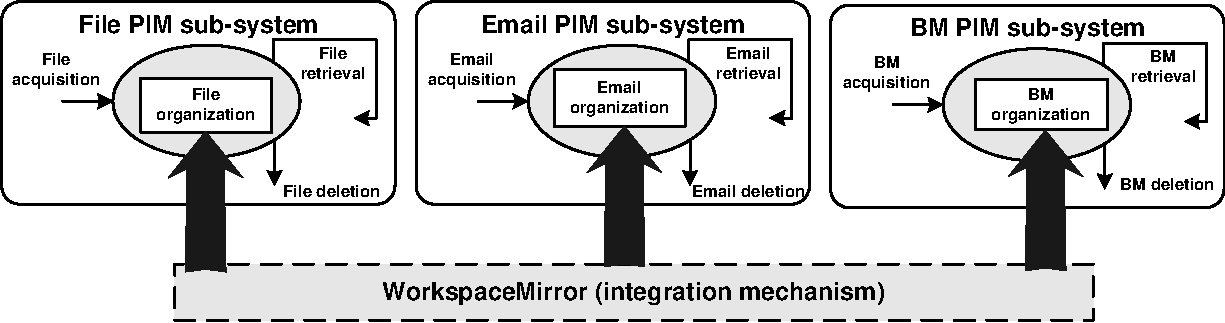
\includegraphics[width=.9 \textwidth]{pictures/discussion/PIM-cross-tool-artefact.pdf}
		% fs-fm-comparison.pdf}
	\end{center}
	\caption{WorkspaceMirror conceptualized as a cross-tool artefact which acts as a design intervention in multiple PIM-tools}
	\label{fig:discussion:ct-artefact}
\end{figure}

% Cross-tool scenarios, as discussed above, may be useful in identifying unforeseen impacts.


% This thesis is a case-study in doing just this.
% uch recommendations are only useful if its influences practice.  
% operationalize
% Rest of thesis is an exercise in putting these methodological suggestions into practice.  This thesis as putting such a cross-tool perspective into operationalization.  Leading into the practical and analytical work to follow, the operationalization of this methodology.
This thesis acts as a case-study to illustrate how many of these recommendations can be put into practice. \textbf{Chapter~\ref{chapter:exploratory_study}} reported a cross-tool study which surveyed user behaviour across files, email and bookmarks.  \textbf{Chapter~\ref{chapter:design}} reported a cross-tool design and implementation based on those requirements. \textbf{Chapter~\ref{chapter:main-study}} reported the cross-tool evaluation of the design.

%%%%%%%%%%%%%%%%%%%%%%%%%%%%%%%%%%%%%%%%%%%%%%%%%%%%%%%%%%%%%%%%%%%%%%%%%%%%%%%%%%%%%%%%%%%%%%%%%%%%%%%%%%%%%%%%%
%%%%%%%%%%%%%%%%%%%%%%%%%%%%%%%%%%%%%%%%%%%%%%%%%%%%%%%%%%%%%%%%%%%%%%%%%%%%%%%%%%%%%%%%%%%%%%%%%%%%%%%%%%%%%%%%%
%%%%%%%%%%%%%%%%%%%%%%%%%%%%%%%%%%%%%%%%%%%%%%%%%%%%%%%%%%%%%%%%%%%%%%%%%%%%%%%%%%%%%%%%%%%%%%%%%%%%%%%%%%%%%%%%%
%%%%%%%%%%%%%%%%%%%%%%%%%%%%%%%%%%%%%%%%%%%%%%%%%%%%%%%%%%%%%%%%%%%%%%%%%%%%%%%%%%%%%%%%%%%%%%%%%%%%%%%%%%%%%%%%%

%%%%%%%%%%%%%%%%%%%%%%%%%%%%%%%%%%%%%%%%%%%%
\subsection{Designing for an Ongoing Activity}
\label{discussion:methodology:ongoing}
%%%%%%%%%%%%%%%%%%%%%%%%%%%%%%%%%%%%%%%%%%%%
%%%%%%%%%%%%%%%%%%%%%%%%%%%
% USE IN METH RECS
% (1) IMPLICS FOR EVAL
% (2) IMPLICS FOR STUDY
%%%%%%%%%%%%%%%%%%%%%%%%%%%

\textbf{Section~\ref{discussion:ongoing}} detailed two longitudinal perspectives from which PIM can be analysed: (1) as a sequence of discrete events, and (2) as a ongoing activity.  Here it is argued that both perspectives can be useful during requirements gathering and evaluation:
 
% Interface design and evaluation: must consider short-term and long-term needs and scenarios.
% In the short-term, efficiency of one-off events may be more important. However, over the long-term satisfaction may be more important based on the long-term perspective.  In the extreme, the lifetime of personal information now extends over the life-time of an individual.  Also the middle ground of acquisition/retrieval pairs and possible interference between them.  
% Consideration of user requirements on both time-scales is encouraged.
\begin{itemize}

\item \textit{Requirements gathering} -- Attention should be paid to both time-scales when assessing user needs.  For example, user needs in the short-term may conflict with those in the long-term. As well as analysing interactions as one-off events, the impact of a design intervention on associated events, such as storage and retrieval, should be considered.   For example, consider the design of a new search mechanism.  In the short-term, the optimization of the efficiency of a discrete individual retrieval event may be paramount.  However, over the long-term, users may want to reuse search requests. This would suggest the need to save and possibly organize those requests. This in turn may increase the time and complexity in making the initial request.

%%%%%%%%%%%%%%%%%%%%%%%%%%%%%%%%%%%%%%%%%%%%%%
% Consider the different PIM sub-activities
%%%%%%%%%%%%%%%%%%%%%%%%%%%%%%%%%%%%%%%%%%%%%%
One useful approach may be to employ a scenario centred on the \textit{life-cycle of a piece of information}.  Tracking interactions with a particular piece of information over time may highlight user issues in terms of a sequence of PIM actions involving all the PIM sub-activities.  
% PIM constitutes a range of sub-activities: acquisition, organization, maintenance, and retrieval.  Therefore, user needs may vary depending on \textit{both} time-scale and sub-activity.  

%%%%%%%%%%%%%%%%%%%%%%%%%%%%%%%%%%%%%%%%%%%%%%%%%%%%%%%%%%%%%
%%%%%%%%%%%%%%%%%%%%%%%%%%%%%%%%%%%%%%%%%%%%%%%%%%%%%%%%%%%%%
%%%%%%%%%%%%%%%%%%%%%%%%%%%%%%%%%%%%%%%%%%%%%%%%%%%%%%%%%%%%%
%%%%%%%%%%%%%%%%%%%%%%%%%%%%%%%%%%%%%%%%%%%%%%%%%%%%%%%%%%%%%
%%%%%%%%%%%%%%%%%%%%%%%%%%%%%%%%%%%%%%%%%%%%%%%%%%%%%%%%%%%%%
% ONGOING: DESIGN IMPLICATIONS
%%%%%%%%%%%%%%%%%%%%%%%%%%%%%%%%%%%%%%%%%%%%%%%%%%%%%%%%%%%%%
Some user needs may only be apparent over the long-term.  For instance, the folder hierarchy is often criticized for not being easily adaptable to fast-changing user needs.  Consequently, requirements for dynamic views of personal information are often emphasized in PIM design, e.g.~\citep{dourish:99a,Dumais:03a}.  A long-term perspective may suggest a contrasting view: that the slow-changing nature of the folder hierarchy may
benefit users by promoting familiarity with the personal information environment. Such familiarity in turn supports location-based finding for which users expressed a clear preference.  Thus, \textit{persistence} is highlighted as an often overlooked, yet desirable design goal.  % Current tools, by their static nature, are good at supporting this design goal.


%%%%%%%%%%%%%%%%%%%%%%%%%%%%%%%
% Evaluate over long-term.  
%%%%%%%%%%%%%%%%%%%%%%%%%%%%%%%
% Participants can take a long time to adjust strategy with a background activity like PIM.  
% Also, first impressions may not reflect long-term behaviour.  In the main study both F3 and M5 changed their mind regarding their opinion of the WM prototype.
\item \textit{Evaluation} -- Evaluation should be performed over the long-term.  The fact that several participants changed their opinion regarding the WM prototype in \textbf{Chapter~\ref{chapter:main-study}} emphasises this point.  Such key observations would not have been revealed in a ``snapshot'' study.  Furthermore, the incremental nature of strategy changes, as reported in \textbf{Chapter~\ref{chapter:main-study}}, means that it may take time for users to adapt to new tools and for stable behaviour to emerge.  % If possible, give users time to adapt their behaviour evolve. % Users may change slowly (especially if don't want to press-gang and bias them).

\end{itemize}

%%%%%%%%%%%%%%%%%
% theory crap
%%%%%%%%%%%%%%%%%
% The theory (UXP model and change/settled model): step towards modelling over long-term, strategy evolution.  Future work: Models exist for short-term IR events.  What about 
%DEVELOPING THEORY:  Theory: step towards modelling over long-term.  UXP
% Most theoretical models relate to the modelling of short-term events.  % is this true for balter? Here, the importance of developing models over the long-term is stressed, such modelling as storage/retrieval event sequences related to one piece of information.  
% Later in this chapter, two long-term models are offered as indications of the kind of work which could usefully be done.  Firstly, a model of strategy changes over time is presented in \textbf{Section X}. Also, a model of user experience over time is presented in \textbf{Section~\ref{discussion:uxp}}.



%%%%%%%%%%%%%%%%%%%%%%%%%%%%%%%%%%%%%%%%%%%%%%%%%%%%%%%%%%%%%%%%%%%%%%%%%%%%%%%%%%%%%%%%%%%%%%%%%%%%%%%%%%%%%%%%%
%%%%%%%%%%%%%%%%%%%%%%%%%%%%%%%%%%%%%%%%%%%%%%%%%%%%%%%%%%%%%%%%%%%%%%%%%%%%%%%%%%%%%%%%%%%%%%%%%%%%%%%%%%%%%%%%%
%%%%%%%%%%%%%%%%%%%%%%%%%%%%%%%%%%%%%%%%%%%%%%%%%%%%%%%%%%%%%%%%%%%%%%%%%%%%%%%%%%%%%%%%%%%%%%%%%%%%%%%%%%%%%%%%%
%%%%%%%%%%%%%%%%%%%%%%%%%%%%%%%%%%%%%%%%%%%%%%%%%%%%%%%%%%%%%%%%%%%%%%%%%%%%%%%%%%%%%%%%%%%%%%%%%%%%%%%%%%%%%%%%%

%%%%%%%%%%%%%%%%%%%%%%%%%%%%%%%%%%%%%%%%%%%%
\subsection{Designing for a Supporting Activity}
\label{discussion:methodology:supporting}
%%%%%%%%%%%%%%%%%%%%%%%%%%%%%%%%%%%%%%%%%%%%

%  due to the provision of information needs by higher-level production activities. 
\textbf{Section~\ref{discussion:supporting}} discussed how PIM is not a self-contained activity.  Instead, it is driven by the production activities which provide the user's information needs.   Such a view suggests that the evaluation of PIM technology should not be limited to measuring improvements in the context of PIM alone.  The effectiveness of how well that PIM-tool supports production activities, may be a useful measure of tool effectiveness. % should also be considered, as well as measures of ongoing user satisfaction.
However, the author notes that such indirect measures of design success may be hard to capture in practice.
% Cross-tool production activities that involve multiple PIM-tools (e.g. starting a major project) may be useful approaches to investigating user requirements from a cross-tool perspective.  They may also be useful in guiding the evaluation of integration designs.

%%%%%%%%%%%%%%%%%%%%%%%%%%%%%
% STUDY:NATURE:SUPPORTING
%%%%%%%%%%%%%%%%%%%%%%%%%%%%%
% for example to help them optimize their PIM strategies
The author also observes that the very notion of PIM as a supporting activity leads to a dilemma for the designers of PIM-tools. As a supporting activity, PIM can both help and hinder production activities.  More time spent on PIM may result in better strategies and higher productivity.  However, there may be a very different consequence of spending more time managing information: distraction from the very production activities that PIM supports. %   -- however, too much PIM may in fact distract the user from what they are meant to be doing.
%\textbf{Section~\ref{discussion:uxp-balance}} describes the implications of PIM's supporting nature for PIM-tool designers, and employers alike.

\begin{itemize}

\item \textit{Encouraging users to spend more time on PIM} -- During the main study, participants reported that they were more focused on PIM due to the author's study and design interventions.  Those participants who changed strategies noted that this increased focus was a key factor in helping them optimize their management style. Although the changes observed in the main study were subtle, participants found them beneficial.  % This suggests that users may benefit from increased reflection on PIM.  

%%%%%%%%%%%%%%%%%%%%%%%%%%%%%%%%%%%%%%
% TO ADD: IMPLICATIONS FOR DESIGNERS
%%%%%%%%%%%%%%%%%%%%%%%%%%%%%%%%%%%%%%
% Encouraging reflection. 
%\item As an alternative to redesigning tools to promote reflection (e.g. providing statistics on time spent filing and searching), organizations could also play a part here. Typically, organizations are more concerned with knowledge management and other strategic IT - whilst PIM is left to the individual. Nevertheless, PIM is a key aspect of employees' activities and has the potential to cause frustration and waste time. Organizations could publicize PIM-related issues, and encourage employees to self-diagnose problems to improve their PIM effectiveness. (DESIGN RECS)
This suggests a potential design route: encourage users to devote more attention to PIM, so they can improve their strategies, and receive the same benefits that resulted from the ``self-auditing'' effect of the study.  As an alternative to redesigning tools to promote reflection (e.g. providing statistics on time spent filing and searching), organizations could also play a part here. Typically, organizations are more concerned with knowledge management and other strategic IT -- whilst PIM is left to the individual.  Nevertheless, PIM is a key aspect of employees' activities and has the potential to cause frustration and waste time.  Organizations could publicize PIM-related issues, and encourage employees to self-diagnose problems to improve their PIM effectiveness.  There may even be a case for PIM training days to recommend guidelines for effective PIM, e.g.~\citep{Allen:03}.  However, managers  should take care not to be overly prescriptive, or they may be seen to be interfering with individuals' preferred style. 
% Which of these people could benefit from increased reflection? 

% \textbf{Section~\ref{main-study:results:reflection}} participants feedback on the pros and cons of increased reflection on PIM.  

\item \textit{The downsides of spending too much time on PIM} -- Some main study participants also noted the downsides of paying increased attention to PIM: that less attention is available for other activities. This raises a challenge for users, managers and designers alike -- they must help the user to \textit{balance} PIM and the production activities that it supports.

The dilemma for PIM-tool designers is discussed further as follows.  Several of the main study participants gave examples of how ticking off to-do items or filing email messages could be highly satisfying, and even act as a therapeutic break from ``real work''.    One can envisage a PIM-tool that is so effectively designed and so satisfying to use, that its users spend all their time managing the information it contains.  Should designers be encouraging users to spend more time on PIM?   Although this may have the benefit of helping the user improve their strategies, there may also be associated costs.  Every extra minute spent on PIM, is a minute taken away from production activities.  A key challenge for designers is to help users find their ``balance point''.  Designers should encourage users to do enough PIM to support their production activities, but not so much to cause distraction from them.

\end{itemize}



% users may benefit from increased attention to PIM, for example to help them optimize their PIM strategies. Such an increase was manifested in the design and study interventions performed in the main study.  
%Lack of reflection (related to changes in strategy observed in main study).
% ADD: Generally people changed slowly







%  (user needs to do enough PIM to support his/her needs, ie. need to be ``active'').  

% This may be ensuring backups are taken (should be automatic of course).
% Relate to design recommendation relating to promotion of reflection

% So is the ultimate PIM-tool one which is totally transparent -- Star Trek computer meets google?
%%%%%%%%%%%%%%%%%%%%%%%%%%%%%%%%%%%%%%%%%%%%%%%%%%%%%%%%%%%%%%%%%%%%%%%%%%%%%%%%%%%%%%%%%%
% The next section moves on to discuss PIM from a second theoretical perspective, that of a \textit{cross-tool} activity.
% \textit{LINK: Used in UXP section}


%%%%%%%%%%%%%%%%%%%%%%%%%%%%%%%%%%%%%%%%%%%%%%%%%%%%%%%%%%%%%%%%%%%%%%%%%%%%%%%%%%%%%%%%%%%%%%%%%%%%%%%%%%%%%%%%%
%%%%%%%%%%%%%%%%%%%%%%%%%%%%%%%%%%%%%%%%%%%%%%%%%%%%%%%%%%%%%%%%%%%%%%%%%%%%%%%%%%%%%%%%%%%%%%%%%%%%%%%%%%%%%%%%%
%%%%%%%%%%%%%%%%%%%%%%%%%%%%%%%%%%%%%%%%%%%%%%%%%%%%%%%%%%%%%%%%%%%%%%%%%%%%%%%%%%%%%%%%%%%%%%%%%%%%%%%%%%%%%%%%%
%%%%%%%%%%%%%%%%%%%%%%%%%%%%%%%%%%%%%%%%%%%%%%%%%%%%%%%%%%%%%%%%%%%%%%%%%%%%%%%%%%%%%%%%%%%%%%%%%%%%%%%%%%%%%%%%%


%%%%%%%%%%%%%%%%%%%%%%%%%%
% \subsection{Summary}
%%%%%%%%%%%%%%%%%%%%%%%%%%
% Lessons which other researchers can take away ...
% Also can consider basing recommendations on nature of PIM (theory), and based on that derive methodological mplications
% Consider separate section with all recommendations collated. 
% SUMMARY POINT: trying to deal with poor epistemic state of PIM/HCI (anti revolutionary design, research-practice gap)
% This section made a number of methodological recommendations. These are used to drive the directions for future work suggested in \textbf{Chapter~\ref{chapter:conclusion}}.


%%%%%%%%%%%%%%%%%%%%%%%%%%%%%%%%%%%%%%%%%%%%%%%%%%%%%%%%%%%%%%%%%%%%%%%%%%%%%%%%%%%%%%%%%%%%%%%%%%%%%%%%%%%%%%%%%
%%%%%%%%%%%%%%%%%%%%%%%%%%%%%%%%%%%%%%%%%%%%%%%%%%%%%%%%%%%%%%%%%%%%%%%%%%%%%%%%%%%%%%%%%%%%%%%%%%%%%%%%%%%%%%%%%
%%%%%%%%%%%%%%%%%%%%%%%%%%%%%%%%%%%%%%%%%%%%%%%%%%%%%%%%%%%%%%%%%%%%%%%%%%%%%%%%%%%%%%%%%%%%%%%%%%%%%%%%%%%%%%%%%
%%%%%%%%%%%%%%%%%%%%%%%%%%%%%%%%%%%%%%%%%%%%%%%%%%%%%%%%%%%%%%%%%%%%%%%%%%%%%%%%%%%%%%%%%%%%%%%%%%%%%%%%%%%%%%%%%



% \input{tex/discussion/chapter7-discussion-strategies}

%%%%%%%%%%%%%%%%%%%%%%%%%%%%
% CHAPTER 7 - DISCUSSION UXP
%%%%%%%%%%%%%%%%%%%%%%%%%%%%
%%%%%%%%%%%%%%%%%%%%%%%%%%%%%%%%%%%%%%%%%%%%%%%%%%%%%%%%%%%%%%%%%%%%%%%%%%%%%%%%%%%%%%%%%%
% Richard Boardman PhD Thesis: Improving Tool Support for Personal Information Management
%%%%%%%%%%%%%%%%%%%%%%%%%%%%%%%%%%%%%%%%%%%%%%%%%%%%%%%%%%%%%%%%%%%%%%%%%%%%%%%%%%%%%%%%%%

%%%%%%%%%%%%%%%%%%%%%%%%%%%%%%%%%%%%%%%%%%%%%%%%%%%%%%%%%%%%%%%%%%%%%%%%%%%%%%%%%%%%%%%%%%
% NATBIB NOTES
%%%%%%%%%%%%%%%%%%%
%\citet{jon90}                ->    Jones et al. (1990) 
%   \citet[chap.~2]{jon90}       ->    Jones et al. (1990, chap. 2)
%   \citep{jon90}                ->    (Jones et al., 1990) 
%   \citep[chap.~2]{jon90}       ->    (Jones et al., 1990, chap. 2) 
%%%%%%%%%%%%%%%%%%%%%%%%%%%%%%%%%%%%%%%%%%%%%%%%%%%%%%%%%%%%%%%%%%%%%%%%%%%%%%%%%%%%%%%%%%
\newpage
%%%%%%%%%%%%%%%%%%%%%%%%%%%%%%%%%%%%%%%%%%%%%%%%%%%%
\section{PIM User Experience}
\label{discussion:uxp}
%%%%%%%%%%%%%%%%%%%%%%%%%%%%%%%%%%%%%%%%%%%%%%%%%%%%

% This section discusses PIM user experience. 
% A simple model is presented to explain some of the observations regarding the level of satisfaction felt by a user towards their current PIM strategies as reflected in their level of organization. 
% \textbf{Section~\ref{discussion:theoretical-framework}} discussed PIM from three theoretical perspectives: as a supporting activity (\textbf{Section~\ref{discussion:supporting}}), as a cross-tool activity (\textbf{Section~\ref{discussion:cross-tool}}), and as an ongoing activity (\textbf{Section~\ref{discussion:ongoing}}).  This section builds on the second and third of these perspectives to develop a model of \textit{long-term user experience} regarding PIM, as reflected in changes in PIM strategy over time.  This based on the change data from \textbf{Chapter~\ref{chapter:main-study}}.
% INTRO: \textbf{Section~\ref{discussion:methodological-discussion}} highlighted the lack of evaluation metrics appropriate for evaluating PIM interfaces.  This section considers the concept of user experience with respect to PIM.  Based on the results from the studies reported in this thesis, a number of possible qualitative evaluation measures are proposed.

%%%%%%%%%%%%%%%%%%%%%%%%%%%%%%%%%%%%%%%%%%%%%%%%%%%%%%%%%%%%%%%%%%%%%%%%%%%%%%%%%%%%%%%%%%%%%%%%%%%%%%%%%%%%%%%%%
%%%%%%%%%%%%%%%%%%%%%%%%%%%%%%%%%%%%%%%%%%%%%%%%%%%%%%%%%%%%%%%%%%%%%%%%%%%%%%%%%%%%%%%%%%%%%%%%%%%%%%%%%%%%%%%%%
%%%%%%%%%%%%%%%%%%%%%%%%%%%%%%%%%%%%%%%%%%%%%%%%%%%%%%%%%%%%%%%%%%%%%%%%%%%%%%%%%%%%%%%%%%%%%%%%%%%%%%%%%%%%%%%%%
%%%%%%%%%%%%%%%%%%%%%%%%%%%%%%%%%%%%%%%%%%%%%%%%%%%%%%%%%%%%%%%%%%%%%%%%%%%%%%%%%%%%%%%%%%%%%%%%%%%%%%%%%%%%%%%%%

%%%%%%%%%%%%%%%%%%%%%%%%%%%%%%%
% \subsection{PIM user experience}
%%%%%%%%%%%%%%%%%%%%%%%%%%%%%%%

%%%%%%%%%%%%%%%%%%%%%%%%%%%%%%%%%%%%%%%%%%%%%%%%
% \subsection{PIM user experience}
%%%%%%%%%%%%%%%%%%%%%%%%%%%%%%%%%%%%%%%%%%%%%%%%
% \label{discussion:uxp-intro}
% Develop ideas on user experience and incorporate ideas from the previous section.
%%%%%%%%%%%%%%%%%%%%%%%%%%%%%%%%%%%%%%%%%%%%%%%%%%%%

% LIMITATIONS OF TRAD MEASURES: 
Traditional measures of usability focus on performance-related metrics of efficiency, accuracy and productivity~\citep{ad:01,preece:02}.  Preece et al. describe a recent shift towards a wider set of design goals related to the concept of \textit{user experience} -- ``what the use of a system feels like to the user''.  They discuss a series of experience-related design goals such as enjoyability and motivation which are hard to assess with traditional measures.  Similarly, \citet{ad:01} argues the importance of user-experience in evaluating designs.  In particular, he highlights the inadequacy of traditional usability measures for many high-level, ongoing tasks such as information retrieval and data analysis.  Dillon notes that in such tasks, efficiency may not be the user's priority.  Furthermore, such tasks do not always have a definite goal, meaning that effectiveness may be hard to define.
% \textit{Also talk about Dillon who urges a focus on satisfaction over efficiency and effectiveness.}  \textit{Focus here on investigating indicators of satisfaction or user experience.}
The author observes that Dillon's arguments also apply to PIM.  \textbf{Section~\ref{exp-study:Results-comparison}} reported observations of ``irrational user behaviour'', such as storing items that are never used.  In such cases, participants were using interfaces in a clearly inefficient manner.  \textbf{Section~\ref{discussion:ongoing}} discussed the ongoing nature of PIM.  Although, effectiveness may be meaningful for discrete one-off PIM events (e.g. moving a folder), it is not clear how the effectiveness of PIM-tool usage can be measured in the long-term.
%%%%%%%%%%%%%%%%%%%%%%%%%%%%%%%%%%%%%%%%%%%%%%%%%%%%%
% Short term contributant of poor user experience
%%%%%%%%%%%%%%%%%%%%%%%%%%%%%%%%%%%%%%%%%%%%%%%%%%%%%
% Previous studies -- impact on self-worth.  Guilt. Why?
%  the user experience of the study participants is considered with respect to PIM.  
This section considers what measures of user experience could be applied in the context of PIM.

Much of the feedback received from the study participants in \textbf{Chapters~\ref{chapter:exploratory_study}} and \textbf{\ref{chapter:main-study}} emphasised \textit{negative user experience} in terms of PIM -- participants liked to moan.  Many complained of the short-term problems they encountered in retrieving, naming, and classifying items. %, e.g. what to do with an item when it belongs in multiple folders, the so-called dilemma of \textit{multiple classification}.  
The effect of such one-off problems may be minor and limited to short-term frustration.  However, if they reoccur, the effects may build up over time leading to negative user experience over the long-term.   %Furthermore, the supporting nature of PIM means that users rarely devote time to planning and executing changes in strategy.  It is suggested here that a lack of serious reflection on PIM, may contribute to negative user experience, by encouraging the acceptance of non-optimal strategies.  Problems may worsen in the background, e.g. as collections become more cluttered. % (PROVIDE EVIDENCE based on F4, M8?) 
The studies provided some evidence of this.  A number of participants reported feeling ashamed or guilty over the state of one or more of their collections\footnote{The reports of shame and guilt may have been exaggerated since the participants were being asked for a guided tour by the author.  However, other studies have also reported this phenomenon, e.g. ~\citep{Bellotti:00}.}.  In the extreme, such feelings may even impact a user's sense of self-worth.


% A key factor in this may be the perception that ``messy equals bad'' resulting from this social value~(Economist:03).  Current tools may exacerbate such a feeling by not auto-tidying old items, and making pro-organizing functionality highly prominent.
% \end{itemize}
%%%%%%%%%%%%%%%%%%%%%%%%%%%%%%%%%%%%
% Problems build up over the long-term
% Poor long-term user experience
%%%%%%%%%%%%%%%%%%%%%%%%%%%%%%%%%%%%
% Becomes a problem, knock-on effect on productivity. Build-up over time.	
% Problems build up over time.  Exacerbated by supporting nature of PIM.  Acceptance of non-optimal strategies by some users.
% BUILD-UP OVER TIME: 
% DESIGN IDEAS
% Do we need to move away from messy equals bad?  Do tools make it worse?
% Design questions include the question of what can be done to help certain user profiles: for example the image-concious? 



%%%%%%%%%%%
% QUESTION
%%%%%%%%%%%
% \textit{Why do some people change? Why is it hard to change?  Look at the empirical data.}
% This section considers the impact of ongoing \textit{user experience} on why people change.
% This section considers why some people encounter such negative user experience.  A simple model is proposed which attempts to explain some of the observations made in \textbf{Chapter~\ref{chapter:main-study}}.
%%%%%%%%%%%%%%%%%%%%%%%%%%%%%%%%%%%%%%%%%%%%%%%%%%%%
% LINK: Summary and connection to where this is used, what direction may be opened up}
%%%%%%%%%%%%%%%%%%%%%%%%%%%%%%%%%%%%%%%%%%%%%%%%%%%%
% METH SUGG: Impact on methodology for evaluation -- have to measure more than just efficiency.  Idea of Friedman's value-based computing. Security, robustness, to look tidy
% Measures of user experience beyond short-term costs (NB: both positive and negative user experience)

The improvement of PIM user experience should be a key concern for the designers of PIM-tools as PIM is a frequent, everyday activity. Therefore, measures of PIM user experience may be a useful qualitative evaluation metric.  A number of aspects of negative PIM user experience which could be observed in interview data are highlighted as follows:
% These considerations may offer routes for developing evaluation criteria for PIM-tools which cater for more than PIM efficiency and effectiveness.  
% Level of security in one's PIM environment may be an important indicator of user satisfaction.  
% \item control Satisfaction-related values of , ``information safety'' may be as important as the time taken to find an item:

\begin{itemize}

%%%%%%%%%%%%%%%%%%%%%%%%
% A: DO TOO LITTLE PIM
%%%%%%%%%%%%%%%%%%%%%%%%
% Do too little PIM (``little'' is subjective taking factors such as personality into account for a specific user), 
% and production activities suffer.  Too little time is spent on PIM, user may lose more items, possibly feels bad about being messy, cue poor user experience.  % Even not backing up.
% \item DO TOO LITTLE PIM 
% Like the some of the study participants in \textbf{Chapter~\ref{chapter:exploratory_study}}, the user may also feel guilty for being messy (poor user experience). 
% (self-perceived, and ``external'') ``being tidy'', ``looking tidy to others'' clutter anxiety of order
\item \textit{Sense of untidiness} -- Constrained by a finite amount of time and attention resources, the user is faced with a dilemma of how much time to spend managing information.  If the user devotes relatively little attention towards PIM, the possible consequences are that they will feel messy or worry that others will see them that way.  The user may also be concerned that their productivity may be impacted if they are unable to find items.  However, the reasons for feeling untidy may be irrational from an efficiency perspective.  For example, having a ``messy'' inbox may not impact user productivity if search is used effectively.  Whether grounded in productivity concerns or not, guilt over messiness still has the potential to cause poor user-experience.  \citet{levy:01} describes such symptoms as ``anxiety of order''. This may be expressed in terms of the user ``feeling untidy'' or ``out of control''.  Such feelings may be exacerbated by the pressure from society to see tidiness as a positive trait~\citep{Economist:03}. % Because PIM is an everyday activity, users feeling this way are continuously faced with the state of their workspace. 

% : ``everyone thinks I'm messy''. % \textit{Such guilt may even over time affect the user's self-image.}


\item \textit{Sense of wasting time} -- In contrast, guilt may also be generated if the user devotes relatively large amounts of time to PIM.  In this case, the user may feel guilty for ignoring his or her production activities.  % More time spent on PIM means less time for production activities, which may also lead to guilt.

%%%%%%%%%%%%%%%%%%%%%%%%%%%%%%
% Do too much PIM (as above), 
%%%%%%%%%%%%%%%%%%%%%%%%%%%%%%
% and production activities suffer.  Too much time is spent on PIM -- a supporting activity -- distracting the user from what they are meant to be doing.
% \item Do too much PIM: 

\end{itemize}

Each of these aspects of negative user experience, may cause the user to feel dissatisfied with their current strategies, and want to adjust them.   Several examples of ``dissatisfaction with current PIM strategies'' are provided in the next section, grounded in observations from the main study.

% Therefore, ``satisfaction with current PIM strategies'', may be a useful indicator of ongoing PIM user experience, as discussed in the following section.




% LINK TO NEXT SECTION: 

%%%%%%%%%%%%%%%%%%%%%%%%%%%%%%%%%%%%%%%%%%%%%%%%%%%%%%%%%%%%%%%%%%%%%%%%%%%%%%%%%%%%%%%%%%%%%%%%%%%%%%%%
%%%%%%%%%%%%%%%%%%%%%%%%%%%%%%%%%%%%%%%%%%%%%%%%%%%%%%%%%%%%%%%%%%%%%%%%%%%%%%%%%%%%%%%%%%%%%%%%%%%%%%%%

%%%%%%%%%%%%%%%%%%%%%%%%%%%%%%%%%%%%%%%%%%%%%%
% BEHAVIOUR either changing or unchanging
%%%%%%%%%%%%%%%%%%%%%%%%%%%%%%%%%%%%%%%%%%%%%%
%%%%%%%%%%%%%%%%%%%%%%%%%%%%%%%%%%%%%%%%%%%%%%%%
\subsection{Satisfaction with Current PIM Strategies}
%%%%%%%%%%%%%%%%%%%%%%%%%%%%%%%%%%%%%%%%%%%%%%%%
\label{discussion:uxp-settled}

%%%%%%%%%%%%%%%%%%%%%%%%%%%%%%%
% CHANGERS AND NON-CHANGERS
%%%%%%%%%%%%%%%%%%%%%%%%%%%%%%%
% People changed (incrementally) or they didn't.
During the main study reported in \textbf{Chapter~\ref{chapter:main-study}},  two types of user were identified, \textit{changers} and \textit{non-changers}, based on whether they changed strategy over the course of the study.  % \textbf{Section~\ref{main-study:discussion:changes-model}} noted that the observed changes consisted of incremental shifts in the relative proportions of information organized with specific low-level strategies.
% ATTITUDE either settled or unstable
% This section considers why some participants changed strategy, and some did not.  And attempts to discuss how ``settledness with current strategies'' can be used as a measure of user experience.
Two participants (F3 and M5) made minor changes to how certain types of information were organized.  The remaining six participants did not make significant changes to their PIM strategies. However, several of these \textit{non-changers} were dissatisfied with their strategies, and expressed the desire to change them in some way.  However, the changes they desired were often seen to be too expensive in terms of time and effort.  

Based on this analysis, two more user types are identified, based on whether users were satisfied with their current strategies.

%%%%%%%%%%%%%%%%%%%%%%%%%%%%%%%%%%%%%%%%%%
% USE IN THEORY DEV: SETTLED/UNSETTLED): 
%%%%%%%%%%%%%%%%%%%%%%%%%%%%%%%%%%%%%%%%%%
% Regarding major shifts in strategy: two user types could be identified based on how content they were with their current set of strategies: settled and unsettled.
\begin{enumerate}
\item \textit{Satisfied with current strategies} -- These users are content with their current management strategies, and do not want to change them. % and are not got down by them on an ongoing basis.

\item \textit{Dissatisfied with current strategies} -- These users are not content with their management strategies, and want to change them in some way.  % However, they may not make the changes due to the perceived costs involved.  % Therefore they may experience this sense of dissatisfaction over the long-term. %  have to live with the dissatisfaction, causing long-term negative user experience.  \textit{This may be a useful indicator of poor user experience.}

% TWO DESIRES: This leads to a desire to: (1) change tool, and (2) change practice.

\end{enumerate}


 

% Changes in strategy are related to user experience
% Propose PIM strategy personalities (stable/unstable-self-punishing)
% It is argued that users who are more unhappy with their strategy and want to change have a worse user experience. 
% there was not a direct correlation between level of organizing and whether users were settled in their strategies.
\textbf{Figure~\ref{fig:discussion:settled-unsettled-model}} presents a series of user profiles which illustrate some examples of ``strategy dissatisfaction''. These are also used to describe observations from the main study in \textbf{Chapter~\ref{chapter:main-study}}.  The horizontal axis indicates whether the user's current organizing behaviour is pro-organizing or organizing-neutral. The vertical axis indicates how satisfied the user feels towards their current strategies.  Note that the figure does not specify a particular tool context.  Five user profiles are identified as follows:
\begin{enumerate}

\item \textit{Profile A: Satisfied and organizing-neutral} -- Profile A has a pragmatic attitude towards PIM.  She considers organization to be low priority, and feels confident that she can find information when she needs it.  % She sees no benefit in filing more information and has ``better things to do''. 
Participant M7 in the main study was an example of this profile in all tool contexts -- he was satisfied with his organizing-neutral strategies and enjoyed positive user experience.
% User A is untidy and could not care less. She has a laid back attitude to clutter

\item \textit{Profile B: Satisfied and pro-organizing} -- Profile B is also satisfied, but is highly organized. She spends a lot of time filing information and believes the time and effort is worth it.  Participants M1, M2, and M6 in the main study were examples of this profile in terms of their file and email practices.  M5 is also considered an example of this profile in files and email.  Although he made pro-organizing changes to his strategies, these were relatively minor.

The remaining three profiles are examples of users who are dissatisfied with their current strategies and consequently suffering poor user experience.

\item \textit{Profile C: Dissatisfied and organizing-neutral} -- Profile C is ``image-concious''.  He considers himself untidy, and feels guilty for not being more organized.  Participant M3 was an example of this profile in his file collection: he devoted relatively little effort to organizing, but talked of the social pressure he faced to be more organized.  He made some pro-organizing changes towards the end of the study.

\item \textit{Profile D: Dissatisfied and pro-organizing}:  Like profile C, profile D is also ``image-concious''.  Although relatively organized, she is still not satisfied with the state of her workspace. Participants M4 and M8 fit this profile in terms of their file management: they both devoted a significant amount of effort to PIM, but wanted to be more organized.  However, both stated that they did not have enough time to perform the significant reorganizing they felt was necessary.  

\item	\textit{Profile E: Dissatisfied and pro-organizing} -- This last profile is a hypothetical example.  None of the study participants matched the profile, however it is included as an interesting example of behaviour.  Profile E devotes significant effort to PIM, but resents the amount of time she spends filing information, seeing it as a waste of time.  She believes that she could benefit by not filing, and instead rely on search like one of her colleagues. However, she is not willing to take the plunge and stop relying on folders.  

\end{enumerate}

%\item pragmatic
%\item image-conscious. Image-concious, ``tidy'' has become a value imposed by society. 

%%%%%%%%%%%%%%%%%%%%%%%%%%%%%%%%%%%%%%
% %%%%%%%%%%%%%%%%%%%%%%%%%%%%%%%%%%%%
% FIGURE - Settled PIM and unsettled PIM
% %%%%%%%%%%%%%%%%%%%%%%%%%%%%%%%%%%%%
%%%%%%%%%%%%%%%%%%%%%%%%%%%%%%%%%%%%%%
\begin{figure}[t]
	\begin{center}
		\leavevmode
		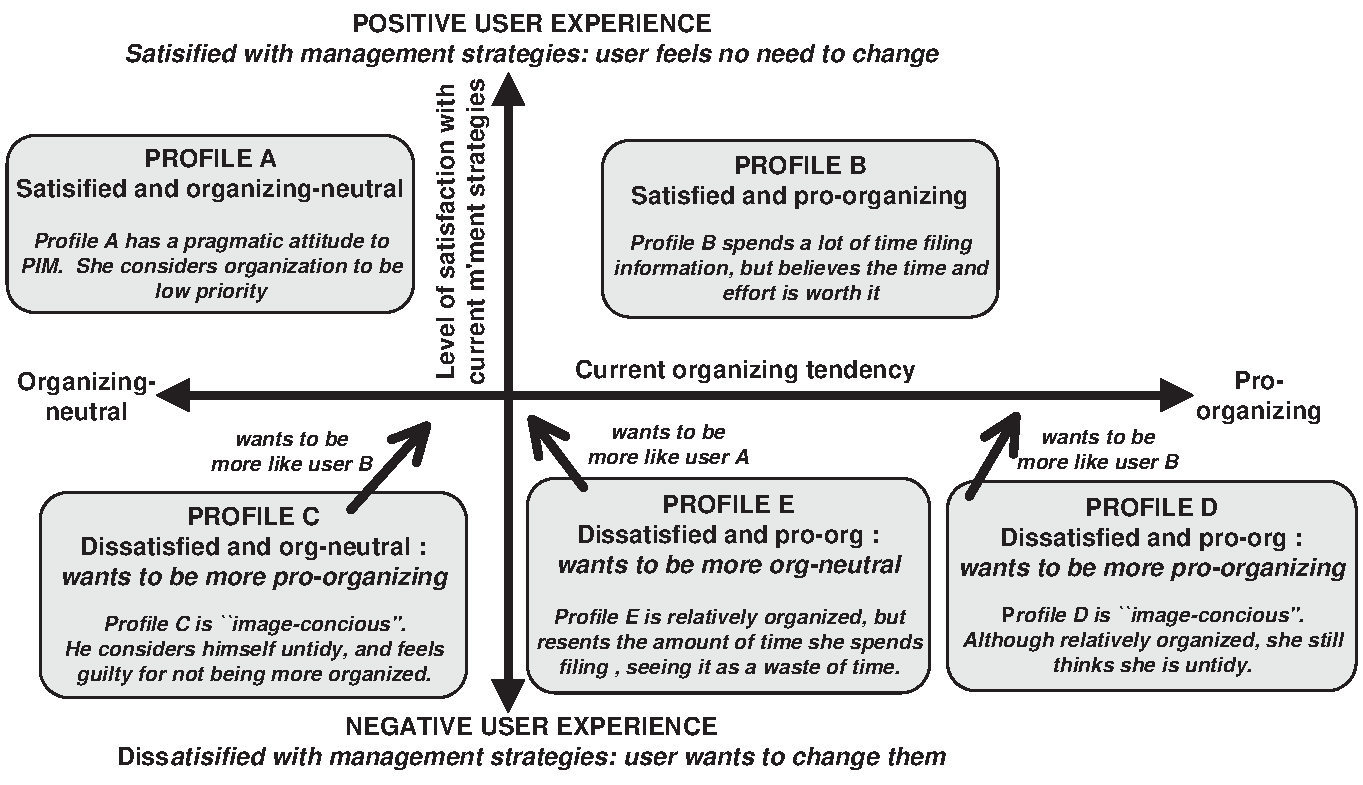
\includegraphics[width=\textwidth]{pictures/discussion/settled-unsettled-model.pdf}
	\end{center}
	\caption{Examples of poor PIM user experience caused by ``dissatisfaction with PIM strategies''}
	\label{fig:discussion:settled-unsettled-model}
\end{figure}

% There may even by a conflict between the two attitudes (organizing-neutral and pro-organizing) for some users.  For example, a user caught between profiles D and E can be envisaged although none was encountered in the process of this research. 
%%%%%%%%%%%%%%%%%%%%%%%%%%%%%%%%%%%%%%%%%%%%%%%%%%%%%%%%%%%%%%%%%%%%%%%%%%%%
% provide examples of both from both pro-org and org-neut perspectives
% The main study provided examples of both settled and unsettled users. 
%%%%%%%%%%%%%%%%%%%%%%%%%%%%%%%%%%%%%%%%%%%%%%%%%%%%%%%%%%%%%%%%%%%%%%%%%%%%
%%%%%%%%%%%%%%%%%%%%%%%%%%%%%%%%%%%%%%%%%%%%%%%%%%%%%%%%%%%%%%%%%%%%%%%%%%%%%%%%%%%%%
%Settled users (examples) of various (high-level) organizing dispositions (pro-org and org-neut), and wanting to shift both ways:
%\begin{itemize}
%	\item Settled and pro-org: M1, M2, M6
%	\item Settled and org-neut: M5, M7
%\end{itemize}
%%%%%%%%%%%%%%%%%%%%%%%%%%%%%%%%%%%%%%%%%%%%%%%%%%%%%%%%%%%%%%%%%%%%%%%%%%%%%%%%%%%%%
%Unsettled users (examples) of both pro-org and org-neut, and wanting to shift both ways:
%\begin{itemize}
%	\item Unsettled, pro-org and wanting to be more pro-org: M4, M8 (mild)
%	\item Unsettled, org-neut and wanting to be more pro-org: M3
%	\item Can one envisage unsettled, pro-org and wanting to be org-neut (yes, if aware wasting lots of time on PIM?)
%\end{itemize}
%%%%%%%%%%%%%%%%%%%%%%%%%%%%%%%%%%%%%%%%%%%%%%%%%%%%%%%%%%%%%%%%%%%%%%%%%%%%%%%%%%%%%
These examples illustrate that users with either pro-organizing or organizing-neutral behaviour may feel dissatisfied with their strategies, and want to change them in some way.  It is hypothesized that an ongoing need to change one's behaviour, combined with an inability to achieve the change, may contribute to poor PIM user experience.  This may be exacerbated if the symptoms which make the user want to perform the change get worse in the meantime.

% In contrast, users who are broadly satisfied with their strategies -- whether organizing-neutral, or pro-organizing -- will not . % THINK: look at what M6 said again
% with their level of balance/their strategies. The author therefore proposes ``satisfaction with management strategies'' as a measure of PIM user experience.  




%%%%%%%%%%%%%%%%%%%%%%%%%%%%%%%%%%%%%%%%%%%%%%%%%%%%%%%%%%%%%%%%%%%%%%%%%%%%%%%%%%%%%%%%%%%%%%%%%%%%%%%%%%%%%%%%%
%%%%%%%%%%%%%%%%%%%%%%%%%%%%%%%%%%%%%%%%%%%%%%%%%%%%%%%%%%%%%%%%%%%%%%%%%%%%%%%%%%%%%%%%%%%%%%%%%%%%%%%%%%%%%%%%%
%%%%%%%%%%%%%%%%%%%%%%%%%%%%%%%%%%%%%%%%%%%%%%%%%%%%%%%%%%%%%%%%%%%%%%%%%%%%%%%%%%%%%%%%%%%%%%%%%%%%%%%%%%%%%%%%%
%%%%%%%%%%%%%%%%%%%%%%%%%%%%%%%%%%%%%%%%%%%%%%%%%%%%%%%%%%%%%%%%%%%%%%%%%%%%%%%%%%%%%%%%%%%%%%%%%%%%%%%%%%%%%%%%%

%%%%%%%%%%%%%%%%%%%%%%%%%%%%%%%%%%%%%%%%%%%%%%%%%%%
% \subsection{Balancing PIM with production tasks}
% \label{discussion:uxp-balance}
%%%%%%%%%%%%%%%%%%%%%%%%%%%%%%%%%%%%%%%%%%%%%%%%%%%
%%%%%%%%%%%%%%%%%%%%%%%%%%%%%%%%%%%%%%%%%%%%%%%%%%%%
% \subsection{Balance model: how much time should users spend on PIM?}
%%%%%%%%%%%%%%%%%%%%%%%%%%%%%%%%%%%%%%%%%%%%%%%%%%%%
% FOUNDATION: supporting nature of PIM, paradox of PIM
%\item \textit{THINK: is this really longitudinal?}
% The study data emphasised the supporting nature of PIM -- to support production activities. 
% A model of PIM and relationship to production activities in terms of the ``need for balance'' (user needs to do enough PIM to support his/her needs, ie. need to be ``active'')
% The supporting nature of PIM leads to a paradox in terms of how much PIM should be performed by a user in support of their production tasks.  The user is faced with a dilemma:
%This section considers the dilemma faced by many users in their PIM activity.  Constrained by a finite amount of time and attention resources, the user is faced with a dilemma of how much time to spend managing information in support of their production tasks:
%\begin{enumerate}

%%%%%%%%%%%%%%%%%%%%%%%%
% A: DO TOO LITTLE PIM
%%%%%%%%%%%%%%%%%%%%%%%%
% Do too little PIM (``little'' is subjective taking factors such as personality into account for a specific user), 
% and production activities suffer.  Too little time is spent on PIM, user may lose more items, possibly feels bad about being messy, cue poor user experience.  % Even not backing up.
%\item If the user devotes relatively little attention towards PIM, the possible consequence is that their production activities may suffer. For example spending little time organizing items, may mean that it is harder to find items in the future.  Like the some of the study participants in \textbf{Chapter~\ref{chapter:exploratory_study}}, the user may also feel guilty for being messy (poor user experience).  The net effect of such problems is that the user's productivity may be impacted.

%%%%%%%%%%%%%%%%%%%%%%%%%%%%%%
% Do too much PIM (as above), 
%%%%%%%%%%%%%%%%%%%%%%%%%%%%%%
% and production activities suffer.  Too much time is spent on PIM -- a supporting activity -- distracting the user from what they are meant to be doing.
%\item However if the user devotes relatively large amounts of time to PIM -- for example by developing a new PIM strategy -- his or her production activities may also suffer.  More time spent on PIM means less time for production tasks, especially in the short-term which the user may be more focused on.
%\end{enumerate}
%This dilemma is represented diagrammatically as the balance model in \textbf{Figure~\ref{fig:discussion:balance-model}}.

%%%%%%%%%%%%%%%%%%%%%%%%%%
% mention user quotes?
%%%%%%%%%%%%%%%%%%%%%%%%%%
% Paradox: if you don't do it, you waste time, all the time you do spent on it, you are wasting time!
% Talk about people who are happy/unhappy and how they fit into the model. 
% Relate to the need for satisficing
% different individuals would tend towards different balance points.  
% Other factors would also come into play.  \textit{How important does user consider organizing to be?}
%This theoretical model can be used as a framework to discuss the varying amounts of effort that different individuals devote to PIM.  \textbf{Chapter~\ref{chapter:exploratory_study}} introduced the terms \textit{pro-organizing} and \textit{organizing-neutral} to describe the level of importance which individuals assigned to being tidy.
% For organizing-neutral users, organising is not important and consequently they may satisfice by not organizing most items.
%Organizing-neutral users may consider even moderate time spent on PIM as a waste.  Therefore they would tend towards a satisficing strategy of only organizing a few items. For them, the balance point is shifted to the right.  % However, this study data suggests that even these users will organize some stuff. 

%However, more pro-organizing users may feel compelled to devote more time to PIM, and feel able to withstand more distraction from their production tasks. \textit{It is has observed that PIM is satisficing~\citep{barreau:95}. However PIM is not satisficing for everyone. For one person, satisficing is the perfect strategy -- they can get away cutting corners. However, for another satisficing may lead to poor user experience as they are continuously faced with this mess which they feel bad about.} % as they can cut corners, and they have to for lack of time buit 



%%%%%%%%%%%%%%%%%%%%%%%%%%%%%%%%%%%%%%
% %%%%%%%%%%%%%%%%%%%%%%%%%%%%%%%%%%%%
% FIGURE - Balancing PIM and production activities
% %%%%%%%%%%%%%%%%%%%%%%%%%%%%%%%%%%%%
%%%%%%%%%%%%%%%%%%%%%%%%%%%%%%%%%%%%%%
%\begin{figure}[t]
%	\begin{center}
%		\leavevmode
%		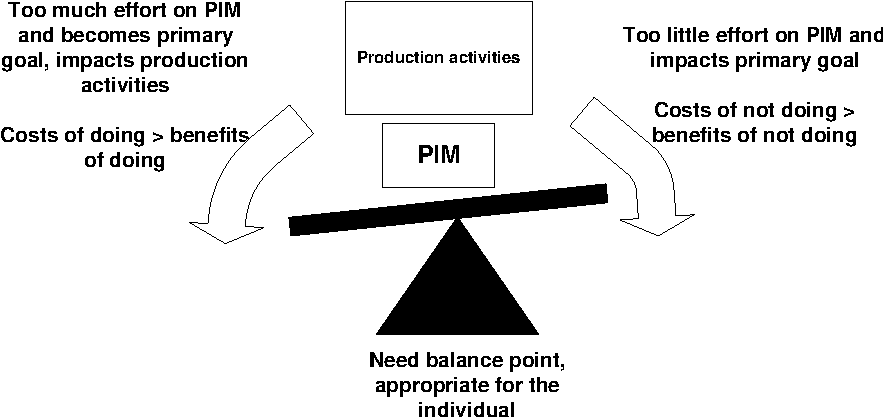
\includegraphics[width=\textwidth]{pictures/discussion/balance-model.pdf}
%	\end{center}
%	\caption{Balancing PIM and production activities}
%	\label{fig:discussion:balance-model}
%\end{figure}


%Lack of reflection (related to changes in strategy observed in main study).
% ADD: Generally people changed slowly
%Although the changes observed in the main study were subtle, participants found them beneficial.  This suggests that users may benefit from some level of reflection on PIM.  However, the supporting nature of PIM means that users rarely devote time to planning and executing changes in strategy.  It is suggested here that a lack of serious reflection on how strategies may be changed, may lead to the acceptance of non-optimal strategies.  Such problems may worsen in the background and/or get worse over time. % (PROVIDE EVIDENCE based on F4, M8?) 

%%%%%%%%%%%%%%%%%%%%%%%%%%%%%%%%%%%%%%
% TO ADD: IMPLICATIONS FOR DESIGNERS
%%%%%%%%%%%%%%%%%%%%%%%%%%%%%%%%%%%%%%
% Encouraging reflection. 
%\item As an alternative to redesigning tools to promote reflection (e.g. providing statistics on time spent filing and searching), organizations could also play a part here. Typically, organizations are more concerned with knowledge management and other strategic IT - whilst PIM is left to the individual. Nevertheless, PIM is a key aspect of employees' activities and has the potential to cause frustration and waste time. Organizations could publicize PIM-related issues, and encourage employees to self-diagnose problems to improve their PIM effectiveness. (DESIGN RECS)
%Users may benefit from increased reflection with respect to PIM, so as to receive the same benefits that resulted from the ``self-auditing'' effect of the study. As an alternative to redesigning tools to promote reflection (e.g. providing statistics on time spent filing and searching), organizations could also play a part here. Typically, organizations are more concerned with knowledge management and other strategic IT - whilst PIM is left to the individual. Nevertheless, PIM is a key aspect of employees' activities and has the potential to cause frustration and waste time. Organizations could publicize PIM-related issues, and encourage employees to self-diagnose problems to improve their PIM effectiveness.  However, managers  should take care not to be overly prescriptive, or interfere with individuals' preferred style. 
% Which of these people could benefit from increased reflection? 

%Also, the balance model proposed above raises a challenge for managers and the purchasers of PIM-tools for organizations. The supporting nature of PIM leads to a second dilemma for users and organizations alike: time spent thinking about PIM may result in distraction from production tasks. Tools and organizations must help the user to balance PIM and the production tasks that it supports.

%And that leads to a dilemma for PIM-tool designers.  In a work context, one can envisage a PIM-tool that is so wonderful to use that people spend all their time using it. Certainly PIM can be fun.  Several participants talked about how to-do ticking or email could be addictive for their personality type.  Should we be encouraging users to spend more time on PIM?   This can have the benefit of improving their strategies.  But at what cost?  Every extra minute spent on PIM, may be taken away from production activities

%  (user needs to do enough PIM to support his/her needs, ie. need to be ``active'').  
%Possibly a suitable aim is to help the user find their ``balance point'', to help them do enough PIM to support their needs, but not to impact their production activities.
% This may be ensuring backups are taken (should be automatic of course).
% Relate to design recommendation relating to promotion of reflection

% So is the ultimate PIM-tool one which is totally transparent -- Star Trek computer meets google?
%%%%%%%%%%%%%%%%%%%%%%%%%%%%%%%%%%%%%%%%%%%%%%%%%%%%%%%%%%%%%%%%%%%%%%%%%%%%%%%%%%%%%%%%%%
% The next section moves on to discuss PIM from a second theoretical perspective, that of a \textit{cross-tool} activity.
% \textit{LINK: Used in UXP section}

%%%%%%%%%%%%%%%%%%%%%%%%%%%%%%%%%%%%%%%%%%%%%%%%%%%%%%%%%%%%%%%%%%%%%%%%%%%%%%%%%%%%%%%%%%%%%%%%%%%%%%%%%%%%%%%%%
%%%%%%%%%%%%%%%%%%%%%%%%%%%%%%%%%%%%%%%%%%%%%%%%%%%%%%%%%%%%%%%%%%%%%%%%%%%%%%%%%%%%%%%%%%%%%%%%%%%%%%%%%%%%%%%%%
%%%%%%%%%%%%%%%%%%%%%%%%%%%%%%%%%%%%%%%%%%%%%%%%%%%%%%%%%%%%%%%%%%%%%%%%%%%%%%%%%%%%%%%%%%%%%%%%%%%%%%%%%%%%%%%%%
%%%%%%%%%%%%%%%%%%%%%%%%%%%%%%%%%%%%%%%%%%%%%%%%%%%%%%%%%%%%%%%%%%%%%%%%%%%%%%%%%%%%%%%%%%%%%%%%%%%%%%%%%%%%%%%%%

%%%%%%%%%%%%%%%%%%%%%%%%%%%%%%%%%%%%%%%%%%
%\subsection{Design recommendations}
%\label{discussion:uxp-design}
%%%%%%%%%%%%%%%%%%%%%%%%%%%%%%%%%%%%%%%%%%



%%%%%%%%%%%%%%%%%%%%%%%%%%%%%%%%%%%%%%%%%%%%%%%%%%%%%%%%%%%%%%%%%%%%%%%%%%%%%%%%%%%%%%%%%%%%%%%%%%%%%%%%%%%%%%%%%
%%%%%%%%%%%%%%%%%%%%%%%%%%%%%%%%%%%%%%%%%%%%%%%%%%%%%%%%%%%%%%%%%%%%%%%%%%%%%%%%%%%%%%%%%%%%%%%%%%%%%%%%%%%%%%%%%
%%%%%%%%%%%%%%%%%%%%%%%%%%%%%%%%%%%%%%%%%%%%%%%%%%%%%%%%%%%%%%%%%%%%%%%%%%%%%%%%%%%%%%%%%%%%%%%%%%%%%%%%%%%%%%%%%
%%%%%%%%%%%%%%%%%%%%%%%%%%%%%%%%%%%%%%%%%%%%%%%%%%%%%%%%%%%%%%%%%%%%%%%%%%%%%%%%%%%%%%%%%%%%%%%%%%%%%%%%%%%%%%%%%

%%%%%%%%%%%%%%%%%%%%%%%
%\subsection{Summary}
%%%%%%%%%%%%%%%%%%%%%%%

%This section has discussed the concept of user experience regarding PIM.

%%%%%%%%%%%%%%%%%%%%%%%%
% FIN: DISCUSSION UXP
%%%%%%%%%%%%%%%%%%%%%%%%

%%%%%%%%%%%%%%%%%%%%%%%%%%%%
% CHAPTER 7 - DISCUSSION CONCLUSION
%%%%%%%%%%%%%%%%%%%%%%%%%%%%
%%%%%%%%%%%%%%%%%%%%%%%%%%%%%%%%%%%%%%%%%%%%%%%%%%%%%%%%%%%%%%%%%%%%%%%%%%%%%%%%%%%%%%%%%%
% Richard Boardman PhD Thesis: Improving Tool Support for Personal Information Management
%%%%%%%%%%%%%%%%%%%%%%%%%%%%%%%%%%%%%%%%%%%%%%%%%%%%%%%%%%%%%%%%%%%%%%%%%%%%%%%%%%%%%%%%%%

% \newpage
%%%%%%%%%%%%%%%%%%%%%%%%%%%%%%%
%%%%%%%%%%%%%%%%%%%%%%%%%%%%%%%
%\subsubsection{Old Conclusion: SCRUB}
%\label{discussion:chapter-summary}
%%%%%%%%%%%%%%%%%%%%%%%%%%%%%%%
%%%%%%%%%%%%%%%%%%%%%%%%%%%%%%%
% Conclusions from the chapter are presented and contributions towards overall thesis are summarized.


%%%%%%%%%%%%%%%%%%%%
% Recap findings
%%%%%%%%%%%%%%%%%%%%
%\textbf{Chapter~\ref{chapter:discussion}} presented a discussion of the findings from the main study.  Here we re-emphasise the main findings from each section.

%\textbf{Section~\ref{discussion:theoretical-framework}} offered a theoretical discussion of three under-researched aspects of PIM: cross-tool, supporting and ongoing.

%\textbf{Section~\ref{discussion:design-guidelines-discussion}} discussed design implications following from the substantive findings in earlier chapters.

%Based on the previous section, \textbf{Section~\ref{discussion:methodological-discussion}} made some methodological recommendations for carrying out research in this area, , based on experiences in carrying out this research.

%\textit{The final two sections, offers models of two aspects of PIM behaviour.  }


%Finally, \textbf{Section~\ref{discussion:uxp}} discusses user experience regarding PIM and offers a possible explanation for some of the long-term problems that users encounter.  Possible measure of user experience for incorporation in tool evaluations are outlined.

%%%%%%%%%%%%%%%%%%%%%
% CONTRIBUTIONS
%%%%%%%%%%%%%%%%%%%%%
%Set out contributions of this chapter towards overall thesis.
%\begin{itemize}
% \item Opened up numerous routes for future work, summarized in \textbf{Chapter~\ref{chapter:conclusion}}. % \textbf{Section~\ref{ch8:research-vistas}}.
%\end{itemize}

%%%%%%%%%%%%%%%%%%%%%%%%%%%%%%%%%%%%%%%%%%%%%%%%%%%%%%%%%%%%%%%%%%%%%%

%%%%%%%%%%%%%%%%%%%%%%%%%%%%%%%
% Signposting
% oving on up: summing up}
%%%%%%%%%%%%%%%%%%%%%%%%%%%%%%%
%The next chapter, Chapter~\textbf{Chapter~\ref{chapter:conclusion}} now concludes the thesis.



%\textit{This draft of Chapter 7 DISCUSSION was printed \today}

%%%%%%%%%%%%%%%%%%%%%%%%%%%%%%
% FIN@ CHAPTER 7 DISCUSSION CONCLUSION AND OVERALL CHAPTER
%%%%%%%%%%%%%%%%%%%%%%%%%%%%%%

%%%%%%%%%%%%%%%%%%%%%%%%%%%%%%%%%%%%%%%%%%%%%%%%%%%%%%%%%%%%%%%%%%%%%%%%%%%%%%%%%%%%%%%%%%%%%%%%%%%%%%%%%%%%%%%%%
%%%%%%%%%%%%%%%%%%%%%%%%%%%%%%%%%%%%%%%%%%%%%%%%%%%%%%%%%%%%%%%%%%%%%%%%%%%%%%%%%%%%%%%%%%%%%%%%%%%%%%%%%%%%%%%%%
%%%%%%%%%%%%%%%%%%%%%%%%%%%%%%%%%%%%%%%%%%%%%%%%%%%%%%%%%%%%%%%%%%%%%%%%%%%%%%%%%%%%%%%%%%%%%%%%%%%%%%%%%%%%%%%%%
%%%%%%%%%%%%%%%%%%%%%%%%%%%%%%%%%%%%%%%%%%%%%%%%%%%%%%%%%%%%%%%%%%%%%%%%%%%%%%%%%%%%%%%%%%%%%%%%%%%%%%%%%%%%%%%%%


%%%%%%%%%%%%%%%%%%%%%%%%%%%%%%%%%%%%%%%%%%%%%%%%%%%%%%%%%%%%%%%%%%%%%%%%%%%%%%%%%%%%%%%%%%%%%%%%%%%%%%%%%%%%%%%%%
%%%%%%%%%%%%%%%%%%%%%%%%%%%%%%%%%%%%%%%%%%%%%%%%%%%%%%%%%%%%%%%%%%%%%%%%%%%%%%%%%%%%%%%%%%%%%%%%%%%%%%%%%%%%%%%%%
%%%%%%%%%%%%%%%%%%%%%%%%%%%%%%%%%%%%%%%%%%%%%%%%%%%%%%%%%%%%%%%%%%%%%%%%%%%%%%%%%%%%%%%%%%%%%%%%%%%%%%%%%%%%%%%%%
%%%%%%%%%%%%%%%%%%%%%%%%%%%%%%%%%%%%%%%%%%%%%%%%%%%%%%%%%%%%%%%%%%%%%%%%%%%%%%%%%%%%%%%%%%%%%%%%%%%%%%%%%%%%%%%%%



%%%%%%%%%%%%%%%%%%%%%%%%%%%%%%%%%%%%%%%%%%%%%%%%%%%%%%%%%%%%%%%%%%%%%%%%%%%%%%%%%%%%%%%%%%%%%%%%%%%%%%%%%%%%%%%%%
%%%%%%%%%%%%%%%%%%%%%%%%%%%%%%%%%%%%%%%%%%%%%%%%%%%%%%%%%%%%%%%%%%%%%%%%%%%%%%%%%%%%%%%%%%%%%%%%%%%%%%%%%%%%%%%%%
%%%%%%%%%%%%%%%%%%%%%%%%%%%%%%%%%%%%%%%%%%%%%%%%%%%%%%%%%%%%%%%%%%%%%%%%%%%%%%%%%%%%%%%%%%%%%%%%%%%%%%%%%%%%%%%%%
%%%%%%%%%%%%%%%%%%%%%%%%%%%%%%%%%%%%%%%%%%%%%%%%%%%%%%%%%%%%%%%%%%%%%%%%%%%%%%%%%%%%%%%%%%%%%%%%%%%%%%%%%%%%%%%%%

%%%%%%%%%%%%%%%%
% METHOD STUFF
%%%%%%%%%%%%%%%%
%%%%%%%%%%%%%%%%%%%%%%%%%
%\subsection{Other stuff to talk about here?}
%%%%%%%%%%%%%%%%%%%%%%%%%
%\begin{itemize}
%	\item User selection
%\end{itemize}


% \textit{CHAPTER 7 LEFT INTENTIONALLY BLANK AS A PLACEHOLDER}



% %%%%%%%%%%%%%%%%%%%%%%%%

% chapter 8 - Conclusion

% %%%%%%%%%%%%%%%%%%%%%%%%

\chapter{Conclusion}

\label{chapter:conclusion}

%%%%%%%%%%%%%%%%%%%%%%%%%%%%
% CHAPTER 8 - CONCLUSION - intro / Research problem and approach
%%%%%%%%%%%%%%%%%%%%%%%%%%%%
%%%%%%%%%%%%%%%%%%%%%%%%%%%%%%%%%%%%%%%%%%%%%%%%%%%%%%%%%%%%%%%%%%%%%%%%%%%%%%%%%%%%%%%%%%%%%
% Richard Boardman PhD Thesis: Improving Tool Support for Personal Information Management
%%%%%%%%%%%%%%%%%%%%%%%%%%%%%%%%%%%%%%%%%%%%%%%%%%%%%%%%%%%%%%%%%%%%%%%%%%%%%%%%%%%%%%%%%%%%%
%%%%%%%%%%%%%%%%%%%%%%%%%%%%%%
%Chapter overview:
%%%%%%%%%%%%%%%%%%%%%%%%%%%%%%
%\begin{enumerate}
%	\item Overall Conclusions
%	\item Review of thesis
%	\item Critical analysis of work (here or discussion?)
%	\item Research Vistas for future work
%	\item Closing words
%\end{enumerate}
%%%%%%%%%%%%%%%%%%%%%%%%%%%%%%%%%%%%%%%%%%%%%%%%%%%%%%%%%%%%%%%%%%%%%%%%%%%%%%%%%%%%%%%%%%%%%
% \textit{NEED: good discussion of EXPLORATORY-ness of the work}
%%%%%%%%%%%%%%%%%%%%%%%%%%%%%%%%%%%%%%%%%%%%%%%%%%%%%%%%%%%%%%%%%%%%%%%%%%%%%%%%%%%%%%%%%%%%%
%What has PhD done towards easing poor epistemic state of PIM/HCI? Modest: hope thaht some useful progress
%%%%%%%%%%%%%%%%%%%%%%%%%%%%%%%%%%%%%%%%%%%%%%%%%%%%%%%%%%%%%%%%%%%%%%%%%%%%%%%%%%%%%%%%%%%%%
%Relate key high-level implications ... key message, pros and cons of integration
%%%%%%%%%%%%%%%%%%%%%%%%%%%%%%%%%%%%%%%%%%%%%%%%%%%%%%%%%%%%%%%%%%%%%%%%%%%%%%%%%%%%%%%%%%%%%
%Future: is PIM as an activity that will fade away a la bookmark management (when we have a google on the desktop)? High level of interest says that it isn't; Bring work up to date: Special interest group co-organized by the author, Signs of increased research interest? -- KFTF, Bergman etc.~\cite{Bergman:03}, RTA (back to basics), number of papers in CHI04, Signs of developer interest, both open-source (Chandler), and commercial (Longhorn)
%%%%%%%%%%%%%%%%%%%%%%%%%%%%%%%%%%%%%%%%%%%%%%%%%%%%%%%%%%%%%%%%%%%%%%%%%%%%%%%%%%%%%%%%%%%%%

%%%%%%%%%%%%%%%%%%
%%%%%%%%%%%%%%%
% LEAD-IN INTRO
%%%%%%%%%%%%%%%
%%%%%%%%%%%%%%%%%%
% This chapter summarises the work presented over the previous seven chapters. %\footnote{\textit{This draft of Chapter 8 CONCLUSION was printed \today}}.
\textbf{Section~\ref{conclusion:recap}} reviews the aims and methodology of the research,  \textbf{Section~\ref{conclusion:contributions}} discusses the contributions offered over the previous seven chapters, and \textbf{Section~\ref{conclusion:critical-reflection}} offers a critical reflection of the thesis.  Finally, \textbf{Section~\ref{conclusion:future-work}} considers future work possibilities.




%%%%%%%%%%%%%%%%%%%%%%%%%%%%%%%%%%%%%%%%
\section{Revisiting the Research Problem and Approach}
\label{conclusion:recap}
%%%%%%%%%%%%%%%%%%%%%%%%%%%%%%%%%%%%%%%%

%%%%%%%%%%%%%%%
% RW PROBLEM
%%%%%%%%%%%%%%%
% Problems in the real world.
% Restate the real-world problem: users have problems managing their information.  
This research has been aimed at improving the HCI knowledge base for the design of the next generation of PIM-tools.  Today's computer users encounter a wide range of problems in managing information, and consequently there is a need to develop improved interfaces to better support this everyday activity.
% ongoing interest in developing improved interfaces.  %The potential of such design is to improve user's productivity and satisfaction in this fundamental aspect of computer-based activity.
%%%%%%%%%%%%%%%%%%%%
% RESEARCH PROBLEM
%%%%%%%%%%%%%%%%%%%%
% However the research that has been carried out in this area has been limited. In particular there has been no systematic investigation of user needs across all three tools, and the potential to unify the tools.  
% As well as a lack of empirical groundwork regarding many aspects of PIM, there has been a particular lack of systematic research in the area of PIM-integration.  
% Thus there is little available guidance for the designers of such tools.  
% There is also a lack of evaluation metrics 
% One possible contributing factor in the lack of evaluation is the scarcity of evaluation methodology appropriate for this type of tool.
The research focused on one specific area of ongoing design interest, that of improving integration between PIM-tools.  As discussed in \textbf{Chapter~\ref{chapter:review}}, previous research relating to this area has been limited.  Although many studies of PIM behaviour have been carried out, few have considered user needs beyond the boundaries of specific tools such as email.  Therefore, there is a lack of empirical foundation for \textit{cross-tool} design work aimed at improving PIM integration.  Consequently, much of the design work in this area has been technologically motivated rather than grounded in user requirements.  However, many of the innovative prototypes that offer new forms of integration have not been evaluated.  Since designers' claims have not been empirically validated, they offer little research value beyond indicating possible routes for design.  % A scarcity of metrics for assessing PIM designs may be one factor contributing to the lack of evaluation.  

%%%%%%%%%%%%%%%%%%%%%%%
% AIM OF THE THESIS
%%%%%%%%%%%%%%%%%%%%%%%
% \textit{Restate the aims and approach of the thesis.} This thesis has sought to investigate how the design of PIM-tools can be improved. Explored potential to unify PIM (must take care with XYZ). Potential of cross-tool approach/methods.
% SET OUT AIMS AS PRE-DEFINED: This thesis was aimed as follows:
\newpage
After assessing the state of prior research in the area, the objectives of this research programme were defined as follows:
\begin{enumerate}

%%%%%%%%%%%%%%%%%%%%
% UNDERSTANDING
%%%%%%%%%%%%%%%%%%%%
% \item To improve understanding of PIM through user studies, to provide empirical guidance for the designers of integration mechanisms.  \textbf{Chapter~\ref{chapter:review}} argued that cross-tool investigation of PIM behaviour was required to provide a thorough empirical foundation for the design of PIM integration mechanisms.
\item \textit{To develop increased understanding of PIM behaviour and needs} -- In particular, the researcher set out to investigate behaviour across multiple PIM-tools, to improve the empirical foundation for the design of PIM-integration mechanisms.   A secondary aim was to develop theoretical models to describe and explain empirical observations.

%%%%%%%%%%%%%%%
% TOOL DESIGN
%%%%%%%%%%%%%%%
% To develop and evaluate a novel PIM-integration mechanism, grounded in empirical motivation.
\item \textit{To design, implement and evaluate a novel PIM-integration mechanism} -- One of the author's key motivations was to develop software to alleviate user problems.  A further intention was to avoid the methodological limitations of previous work by emphasising empirical grounding and evaluation.

 %%%%%%%%%%%%%%%%%
% METHODOLOGICAL
%%%%%%%%%%%%%%%%%
% Methodological: Explore potential of cross-tool approach for both researchers and designers of cross-tool approach. Evaluation: explore ways of doing effective evaluation.  To explore issues related to the evaluation of PIM designs, particularly those directed at improving PIM integration.
% regarding appropriate methodology
% devise appropriate methodology to support the above objectives of investigating PIM, and designing and evaluating PIM-integration mechanisms.  Furthermore, based on these experiences, to produce a set of recommendations regarding the design of PIM interfaces, particularly those aimed at improving PIM integration.
\item \textit{To develop methodological recommendations for future design work} -- The final objective was to provide guidance for future design and evaluation in this area. It was envisaged that the experience of designing and evaluating the PIM-integration prototype would allow the development of such guidelines.

%  provide methodological guidance for future work, derived from the experience of pursuing this course of research.  In particular, \citet{Whittaker-rta:00} note the need for the identification of evaluation metrics.

\end{enumerate}

To achieve these aims a the research methodology was structured on a three-stage process of user-centred design: (1) requirements gathering, (2) design, and (3) evaluation:  

% (1) requirements gathering through an exploratory study, (2) design and implementation, and (3) a 
 
\begin{enumerate}

%%%%%%%%%%%
% APPROACH
%%%%%%%%%%%
%%%%%%%%%%%%%%
% FIRST STAGE
%%%%%%%%%%%%%%
% \item The cross-tool investigation of PIM behaviour across three PIM-tools -- files, email and bookmarks -- reported in \textbf{Chapter~\ref{chapter:exploratory_study}}
%, managed within the file system, email tool, and web browser respectively.
% DIANE: not too much detail here
% Tio provide evidence/description
% Requirements will be gathered through a cross-tool study to build cross-tool understanding of PIM, and so provide an empirical foundation for cross-tool design work aimed at improving PIM integration. The study methodology will consist of semi-structured interviews as used in previous empirical work in this area. The aim is to compare how individuals manage a range of types of personal information, to investigate the effectiveness of current forms of integration, and so as support the generation of empirically-grounded ideas of how further integration can be provided.
\item \textit{Requirements gathering} -- The exploratory study, reported in \textbf{Chapter~\ref{chapter:exploratory_study}}, investigated user behaviour across three PIM-tools -- files, email and bookmarks.  This enabled the comparison of behaviour between the tools, and the exploration of  potential routes for integration.  % \textbf{Chapter~\ref{chapter:exploratory_study}} details the study which compares PIM practices across 3 collections of personal information: personal files, email, and web bookmarks. 

%%%%%%%%%%%%%%%%%%
% SECOND STAGE
%%%%%%%%%%%%%%%%%%
% \item The design and implementation of a new PIM-integration mechanism based on the concept of folder-mirroring (reported in \textbf{Chapter~\ref{chapter:design}}),
\item \textit{Design and prototyping} -- \textbf{Chapter~\ref{chapter:design}} described the design of a PIM-integration mechanism which allows the user to share folder structures between different collections. The design was motivated by the observation of significant folder overlap for many participants in the exploratory study. Also, the design approach was deliberately \textit{incremental} to facilitate systematic evaluation, and cause minimum disruption to users.  % ,   % Findings from the exploratory study are used to motivate the design and implementation of a prototype PIM-integration mechanism.  % The prototype was proposed as a research vehicle to enable the investigation of general issues relating to PIM integration during a field study.
% The design was prototyped so as to embody specific design hypotheses that express intended improvements.
% The findings from the exploratory study will provide the grounding for the design of an interface providing enhanced PIM integration. 
% the design may be a new form of integration or modify an existing form
%% contrast with unification systems that unify and propose a new organizational paradigm. I just do one

%%%%%%%%%%%%%%%%%%
% THIRD STAGE
%%%%%%%%%%%%%%%%%%
%  \item A field study investigation of PIM, encompassing the longitudinal evaluation of the folder-mirroring mechanism (reported in \textbf{Chapter~\ref{chapter:main-study}}).   % \textit{Recap justification of the approach.}
\item \textit{Evaluation} -- \textbf{Chapter~\ref{chapter:main-study}} reported the third stage of the research, the field-study based evaluation of the designed prototype.  The evaluation facilitated the assessment of the specific design, as well as the development of guidelines for the wider PIM design genre.  The field study also enabled the investigation of long-term user behaviour such as changes in organizing strategies over time. 
% Note that the field study also facilitates the investigation of long-term aspects of PIM such as changes in strategy over time. Such longitudinal aspects of PIM have received little attention to date.
% Since no evaluations of this type have been carried out, an important part of this work is the development of appropriate methodology, both for evaluating PIM-tools in general, but also for evaluating means of integration.
% Finally the main study also allowed the investigation of appropriate methodology for evaluating PIM tools.
% Do these really go together? Maybe bring out in the discussion - rather than as an up-front aim!
% Finally the effectiveness of the design will be investigated through a field study-based evaluation.
%% to assess impact of the design intervention
% \item The iterative process of study, design and evaluation provided a platform for theory-building.

\end{enumerate}


% This approach both matched the research aims, and also allowed him to get a first-hand appreciation of real-world design issues.


%%%%%%%%%%%%%%%%%%%%%%%%%%%%%
%\section{Thesis tour/summary}
%%%%%%%%%%%%%%%%%%%%%%%%%%%%%
%
%Firstly, \textbf{Chapter~\ref{chapter:bg}} did X and Y.






%%%%%%%%%%%%%%%%%%%%%%%%%%%%
% CHAPTER 8 - CONCLUSION - Contributions
%%%%%%%%%%%%%%%%%%%%%%%%%%%%
%%%%%%%%%%%%%%%%%%%%%%%%%%%%%%%%%%%%%%%%%%%%%%%%%%%%%%%%%%%%%%%%%%%%%%%%%%%%%%%%%%%%%%%%%%%%%
% Richard Boardman PhD Thesis: Improving Tool Support for Personal Information Management
%%%%%%%%%%%%%%%%%%%%%%%%%%%%%%%%%%%%%%%%%%%%%%%%%%%%%%%%%%%%%%%%%%%%%%%%%%%%%%%%%%%%%%%%%%%%%

\newpage
%%%%%%%%%%%%%%%%%%%%%%%%%%%%%%
%%%%%%%%%%%%%%%%%%%%%%%%%%
\section{Contributions}
\label{conclusion:contributions}
%%%%%%%%%%%%%%%%%%%%%%%%%%
%%%%%%%%%%%%%%%%%%%%%%%%%%%%%%
%	\item Contributions (substantive and methodological)
% Set out contributions of this chapter towards overall thesis -- consider achievements in light of objectives.
%%%%%%%%%%%%%%%%%%%%%%%%%%%%%%%%%%%%%%%%%%%%%%%%%%%%%%%%%%%%%%%%%%%%%%%
%\item Consider achievements in light of objectives
%\item to sum up/tie together/pull together conclusions and contributions from this work
% \item \textit{THINK: ensure contributions here match with those in introduction}
%%%%%%%%%%%%%%%%%%%%%%%%%%%%%%%%%%%%%%%%%%%%%%%%%%%%%%%%%%%%%%%%%%%%%%%
%\item Relate to aims. Do the contributions of the thesis meet those aims? Relate progress/findings towards tackling aims (this is a repeat of the contributions, no?) Have I tackled it? No, not fully - but hopefully taken some steps towards doing so ... (-; Honest, realistic, assessment of my contributions
%%%%%%%%%%%%%%%%%%%%%%%%%%%%%%%%%%%%%%%%%%%%%%%%%%%%%%%%%%%%%%%%%%%%%%%
%\item expand on how they contribute to the HCI knowledge base and why they are valid
%%%%%%%%%%%%%%%%%%%%%%%%%%%%%%%%%%%%%%%%%%%%%%%%%%%%%%%%%%%%%%%%%%%%%%%
%\item What are the implications of the now validated thesis?
%%%%%%%%%%%%%%%%%%%%%%%%%%%%%%%%%%%%%%%%%%%%%%%%%%%%%%%%%%%%%%%%%%%%%%%
% This section reviews the contributions made over the preceding chapters.
Firstly, key contributions are highlighted in \textbf{Section~\ref{conclusion:contributions:key}}. The next two sections detail all the contributions made in this thesis.  \textbf{Section~\ref{conclusion:contributions:understanding}} presents contributions resulting from the study components of the thesis.  Then, \textbf{Section~\ref{conclusion:contributions:design}} discusses contributions resulting from the design, implementation and evaluation of the WorkspaceMirror prototype.

%%%%%%%%%%%%%%%%%%%%%%%%%%%%%%%%%%%%%%%%%%%%%
\subsection{Summary of Key Contributions}
\label{conclusion:contributions:key}
%%%%%%%%%%%%%%%%%%%%%%%%%%%%%%%%%%%%%%%%%%%%%
This thesis offers a variety of contributions.  Here the most significant contributions are highlighted.

The study components of the thesis offer a significant advance over previous work through the investigation of PIM (1) across multiple tools, and (2) over time, thus enabling the development of richer understanding. \textbf{Chapter~\ref{chapter:exploratory_study}} compared PIM behaviour across file, email and bookmark collections, and developed \textit{improved classifications of management strategies}. In particular, it was shown how many users employ multiple organizing strategies, both within and between distinct PIM-tools. In turn,  \textbf{Chapter~\ref{chapter:main-study}} collected data over time, leading to the \textit{development of an improved model of changes in organizing strategies}. The knowledge cultivated in the two studies lead in \textbf{Chapter~\ref{chapter:discussion}} to \textit{the enhancement of Barreau's PIM model to accommodate the cross-tool, supporting and ongoing nature of PIM}.

Other contributions result from the design component of the thesis.  The key contributions in this area include the \textit{design of the WorkspaceMirror prototype}, in \textbf{Chapter~\ref{chapter:design}}, driven by observations of folder overlap in  \textbf{Chapter~\ref{chapter:exploratory_study}}. The \textit{evaluation of the design} in \textbf{Chapter~\ref{chapter:main-study}} confirmed the promise of mirroring top-level folders. This represents one of the few systematic, longitudinal evaluations of a PIM-tool performed to date. The evaluation resulted in the \textit{development of a series of design recommendations}, primarily the importance of recognizing that a PIM-integration mechanism may have strengths and weaknesses in different tool contexts. In addition, a number of \textit{methodological recommendations} were developed including the need to evaluate all PIM designs in both tool-specific and cross-tool perspectives.

The next two sections provide more detail on the contributions from the study and design/evaluation components of the thesis.

% \textbf{Table~\ref{table:conclusion:contributions}} presents an overview of the contributions.
%%%%%%%%%%%%%%%%%%%%%%%%%%%%
% Contribution categories
%%%%%%%%%%%%%%%%%%%%%%%%%%%%
%THINK: two alternatives structures here: substantive versus methodological or divide up in terms of the main offerings:
%Firstly, \textbf{Section~\ref{conclusion:substantive-contributions}} details the substantive contributions, and then  \textbf{Section~\ref{conclusion:methodological-contributions}} details the methodological contributions.
% \item Main contributions, divide as substantive/methodological, major/minor, and audience (researchers/designers):
%The contributions are discussed in terms of the following two categories:
%\begin{enumerate}
% \item Theory/model building to describe/explain subsets of the empirical findings.
%\item Improving understanding of PIM (see )
%\item Design, implementation and evaluation of a novel PIM-integration mechanism (see )
%\end{enumerate}

% The following sections focus on each of these categories in turn.



%%%%%%%%%%%%%%%%%%%%%%%%%%%%%%%%%%%%%%%%%%%%%%%%%%%%%%%%%%%%%%%%%%%%%%%%%%%%%%%%%%%%%%%%%%%%%%%%%%%%%%%%%%%%%%%%%
%%%%%%%%%%%%%%%%%%%%%%%%%%%%%%%%%%%%%%%%%%%%%%%%%%%%%%%%%%%%%%%%%%%%%%%%%%%%%%%%%%%%%%%%%%%%%%%%%%%%%%%%%%%%%%%%%
%%%%%%%%%%%%%%%%%%%%%%%%%%%%%%%%%%%%%%%%%%%%%%%%%%%%%%%%%%%%%%%%%%%%%%%%%%%%%%%%%%%%%%%%%%%%%%%%%%%%%%%%%%%%%%%%%
%%%%%%%%%%%%%%%%%%%%%%%%%%%%%%%%%%%%%%%%%%%%%%%%%%%%%%%%%%%%%%%%%%%%%%%%%%%%%%%%%%%%%%%%%%%%%%%%%%%%%%%%%%%%%%%%%

%%%%%%%%%%%%%%%%%%%%%%%%%%%%%%%%%%%%%%%%%%%%%
\subsection{Improved Knowledge of PIM}
\label{conclusion:contributions:understanding}
%%%%%%%%%%%%%%%%%%%%%%%%%%%%%%%%%%%%%%%%%%%%%
%Theory/models to explain/describe PIM
%\begin{itemize}
%\item Extension of Barreau's model to produce framework encompassing cross-tool, supporting, ongoing aspects of PIM   
%\item Model of multiple strategies in TS/CT contexts
%\item Model of changes in PIM strategies (applied to explaining so rate of take-up of many PIM-tools)
%\item Model of user experience.
%\end{itemize}

This section details contributions that relate to the first aim of the thesis: to develop increased understanding of PIM behaviour.  \textbf{Table~\ref{table:conclusion:contributions:understanding}} provides a summary of the empirical, methodological and theoretical contributions in this area.

%%%%%%%%%%%%%%%%%%%%%%%%%%%%%%%%%%%%%%%%%%%%%%%%%%%%%%
% TABLE: contributions providing increased understanding of PIM
%%%%%%%%%%%%%%%%%%%%%%%%%%%%%%%%%%%%%%%%%%%%%%%%%%%%%%
\begin{table}[hbtp]
\begin{center}
\begin{footnotesize}
\setlength{\extrarowheight}{2pt}
\begin{tabular}{|c|p{9cm}|p{3cm}|}
\hline
{\bf Chapter} & {\bf Contribution} & {\bf Type of contribution} \\
\hline
         2 & Definitions and PIM conceptual framework & theoretical \\
\hline
         3 & Critical review of previous work & theoretical \\
\hline
         4 & Comparison of PIM behaviour between file, email and bookmark collections & empirical findings \\
\hline
         4 & New classifications of organizing strategies in file, email and bookmark collections & empirical findings \\
\hline
         4 & Comparison of organizing strategies between files, email and bookmarks & empirical findings \\
\hline
         4 & Development and application of method to analyse folder structures in terms of \textit{organizational dimensions} & methodological, empirical findings \\
\hline
         4 & Development and application of method to compare folder structures in terms of \textit{folder overlap} & methodological, empirical findings \\
\hline
         4 & Model of multiple PIM strategies within tool-specific and cross-tool contexts & theoretical model \\
\hline
         6 & Insights into longitudinal PIM behaviour: (1) PIM strategy changes, and (2) supporting nature of PIM & empirical findings \\
\hline
         6 & Model of incremental changes in organizing strategy & theoretical \\
\hline
         7 & Extended conceptual framework of PIM illustrating its cross-tool, supporting, ongoing nature & theoretical \\
\hline
         7 & Discussion of qualitative measures of PIM user experience, including ``satisfaction with current strategies'' & theoretical \\
\hline
\end{tabular}  
\end{footnotesize}
\caption{Contributions providing increased understanding of PIM}
\label{table:conclusion:contributions:understanding}
\end{center}
\end{table}
\normalsize

Two studies of PIM behaviour were reported.  Firstly, \textbf{Chapter~\ref{chapter:exploratory_study}} reported an exploratory study in which a semi-structured interview methodology was employed to investigate PIM behaviour across three tools: files, email and bookmarks.   Secondly, \textbf{Chapter~\ref{chapter:main-study}} reported a follow-up longitudinal field study, again across the three tools. As well as investigating PIM behaviour over time, the field study also acted as a research vehicle to evaluate the WorkspaceMirror prototype.  Both studies are distinguished from previous work by their cross-tool nature.

% \subsubsection{Contributions from Chapter 4}
% \item The primary aim of the study was to investigate PIM behaviour between the three tools to develop an empirical foundation for the design of PIM-integration mechanisms).  
% \item Tool-specific insights, e.g. strategy classifications
% in both \textit{tool-specific} and \textit{cross-tool} contexts.  
The primary contribution from \textbf{Chapter~\ref{chapter:exploratory_study}} was \textit{a comparison of PIM-behaviour between files, email and bookmarks} in the terms of four PIM sub-activities: acquisition, organization, maintenance, and retrieval. A number of similarities were noted between the tools including: (1) a preference for browsing-based retrieval over search in all three tool contexts, and (2) the importance of older items for many participants\footnote{These contributions, although minor, add to existing HCI knowledge in each tool-specific context, as well as contributing new cross-tool knowledge.}.  However, some major differences in behaviour were also noted.  These included: (1) the relative unimportance of the bookmark collection, and (2) the uncontrolled nature of acquisition in email.

The rest of \textbf{Chapter~\ref{chapter:exploratory_study}} focused on the organizing sub-activity.  The next contribution was \textit{a comparison of each individuals' organizing strategies across the three tools}. Previous strategy analysis has been limited to specific tools such as email and this is the first attempt to analyse strategies from a cross-tool perspective.  The comparison of organizing strategies between files, email and bookmarks firstly necessitated the characterization of strategies in individual tools. Multiple low-level organizing strategies were observed for many participants in all three tool contexts. Three \textit{new tool-specific strategy classifications} were offered to reflect this behaviour.  Previous classifications were criticised for not capturing this level of detail.  Then, at the cross-tool level, \textit{multiple organizing strategies} were observed for many individuals, as in specific tools.  This confirmed that users do not employ consistent strategies across different collections of personal information.  A number of causal factors were identified including the relative value of the information in each collection -- since files are valued most highly, and are most likely to be retrieved, they are seen to be most worth organizing.  \textit{A theoretical model of multiple strategies} was developed to describe the tool-specific and cross-tool observations of multiple strategies. % , and improve conceptualization of the term ``PIM strategy''. % Previous classifications of user behaviour were criticised for only providing abstractions of actual behaviour. 

% However, a number of \textit{tool-specific contributions} were also made.   % Also, the description of users as ``spring cleaners'' was shown to be inaccurate, as this strategy was only observed in combination with other strategies.
% Study Results. Findings from combined Cross-tool Studies- theoretical insight into what PIM is. Provide further understanding of PIM from a holistic "cross-tool" perspective. 
% , and perhaps the most significant, was the comparison of PIM behaviour between the three tools, incorporating all the data collected above.
%\item 
%\end{itemize}

% Finally, a method of \textit{cross-tool strategy profiling} was proposed and employed to correlate organizing behaviour between the three tools. Previous strategy analysis has been limited to specific tools such as email and this is the first attempt to analyse strategies form a cross-tool perspective.  Again it was seen that many users employ \textit{multiple strategies} in terms of organizing behaviour, and a number of causal factors were identified.
% The next three contributions from \textbf{Chapter~\ref{chapter:exploratory_study}} focus on comparing organizing behaviour between files, email and bookmarks:

%\begin{itemize}
%
%\item 
\textbf{Chapter~\ref{chapter:exploratory_study}} also reported the development and application of two new techniques for comparing organizing behaviour between collections:

\begin{itemize}

\item \textit{A technique for analysing folder structures in terms of the organizational dimensions} -- An analysis of the aggregated data characterized the most common dimensions in each tool context.  Although projects and roles were the most common dimensions observed, a wide range of organizational dimensions were employed.  This lead to the criticism of prototypes such as the \textit{Personal Role Manager}~\citep{Shneiderman:94}, which enforce a dominant organizational dimension. This data suggests that such designs would require users to significantly change their current behaviour.

\item \textit{A technique for assessing the level of \textit{folder overlap} between a participant's file, email and bookmark structures} --  Significant overlap was observed for many participants, particularly between the file and email folder structures.  This observation provided the key empirical motivation for the development of the WM prototype in \textbf{Chapter~\ref{chapter:design}}.  % itemize relating to the design and evaluation of WM are discussed in \textbf{Section~\ref{conclusion:contributions:design}}.

\end{itemize}

%%%%%%%%%%%%%%%%%%%%%%%%%%%%%%%%%%%%%%%%%%%%
% \subsubsection{Contributions from Chapter 6}
%%%%%%%%%%%%%%%%%%%%%%%%%%%%%%%%%%%%%%%%%%%%

% Changes in PIM	%%%%%%%%%%%%%%%%%%%%%%%%%%%%%%%%
% Two main empirical contributions from CHAPTER 6
%%%%%%%%%%%%%%%%%%%%%%%%%%%%%%%%%%%%%%%%%%%%%%%%%%%
The field study in \textbf{Chapter~\ref{chapter:main-study}} offered two further empirical contributions:

\begin{itemize}

\item \textit{The observation of the incremental nature of changes in organizing strategy} -- Tracking PIM behaviour over time revealed that few study participants made significant changes in how they organized information in any of the collections.  Only two participants were observed making strategy changes, which were of a subtle, incremental nature.  Previous theory in the area was criticised for portraying strategy changes in terms of global swings in overall organizing behaviour~\citep{ob:97}.  This data was combined with the model of multiple strategies to develop \textit{a model of changes in organizing strategy} which reflected their incremental nature.  

\item \textit{The identification of the supporting, background nature of PIM} -- This was based on participants' comments that they devoted relatively little attention to PIM compared to their work tasks.  Both the study and design interventions caused many participants to report increased reflection on their PIM strategies.

\end{itemize}

%%%%%%%%%%%%%%%%%%%%%%%%%%%%%%%%%%%%%%%%%%%%
% \subsubsection{Contributions from Chapter 7}
%%%%%%%%%%%%%%%%%%%%%%%%%%%%%%%%%%%%%%%%%%%%

The discussion presented in \textbf{Chapter~\ref{chapter:discussion}} lead to two final contributions in this area:

\begin{itemize}

\item \textit{An extended theoretical framework describing the cross-tool, supporting, and ongoing nature of PIM} --  This framework offers several advances over previous theory in the area, including: (1) a conceptualization of PIM-integration mechanisms which bridge between distinct PIM-tools, and (2) the representation of the relationship between PIM and the production activities it supports.  The framework was used to identify routes for theoretical development in the area.

\item \textit{Discussion of PIM user experience} -- A number of qualitative measures of PIM user experience were offered as alternatives to traditional performance-focused evaluation metrics, which it was argued are inappropriate for activities such as PIM.  A focus was taken on ``dissatisfaction in strategies'' as a key source of poor user experience. Several participants expressed dissatisfaction with their current strategies, but did not change them because of the perceived costs involved.  This data was used to illustrate the forms that such dissatisfaction could take.  

% This and a number of other   % A model of the relationship between user experience and strategy changes was proposed and lead to the identification of a number of \textit{user-experience based evaluation criteria}.

\end{itemize}

%%%%%%%%%%%%%%%%%%%%%%%%%%%%%%%%%%%%%%%%%%%%%%%%%%%%%%%%%%%%%%%%%%%%%%%%%%%%%%%%%%%%%%%%%%%%%%%%%%%%%%%%%%%%%%%%%
%%%%%%%%%%%%%%%%%%%%%%%%%%%%%%%%%%%%%%%%%%%%%%%%%%%%%%%%%%%%%%%%%%%%%%%%%%%%%%%%%%%%%%%%%%%%%%%%%%%%%%%%%%%%%%%%%
%%%%%%%%%%%%%%%%%%%%%%%%%%%%%%%%%%%%%%%%%%%%%%%%%%%%%%%%%%%%%%%%%%%%%%%%%%%%%%%%%%%%%%%%%%%%%%%%%%%%%%%%%%%%%%%%%
%%%%%%%%%%%%%%%%%%%%%%%%%%%%%%%%%%%%%%%%%%%%%%%%%%%%%%%%%%%%%%%%%%%%%%%%%%%%%%%%%%%%%%%%%%%%%%%%%%%%%%%%%%%%%%%%%

%%%%%%%%%%%%%%%%%%%%%%%%%%%%%%%%%%%%%%%%%%%%%
\subsection{Design, Implementation and Evaluation}
\label{conclusion:contributions:design}
%%%%%%%%%%%%%%%%%%%%%%%%%%%%%%%%%%%%%%%%%%%%%

% Grounded design and implementation of WorkspaceMirror as research vehicle to investigate issues involved in improving integration between PIM-tools. 
% Cross-tool design of WorkspaceMirror and its implementation. 
% Knowledge in artifact implementation. Explicitation of knowledge as claims? Other designs?
The second main area of contribution resulted from the design, implementation, and evaluation of the WorkspaceMirror prototype (abbreviated to WM).  \textbf{Table~\ref{table:conclusion:contributions:design}} provides an overview.


%%%%%%%%%%%%%%%%%%%%%%%%%%%%%%%%%%%%%%%%%%%%%%%%%%%%%%
% TABLE: design/implementation contributions
%%%%%%%%%%%%%%%%%%%%%%%%%%%%%%%%%%%%%%%%%%%%%%%%%%%%%%
\begin{table}[hbtp]
\begin{center}
\begin{footnotesize}
\setlength{\extrarowheight}{2pt}
% Table generated by Excel2LaTeX from sheet 'DESIGN-EVAL'
\begin{tabular}{|c|p{9cm}|p{3cm}|}
\hline
{\bf Chapter} & {\bf Contribution} & {\bf Type of contribution} \\
\hline
         5 & Design and implementation of WorkspaceMirror (WM) & design and implementation \\
\hline
         5 & Results from the initial evaluation of WM & empirical findings \\
\hline
         6 & Results from the field-study longitudinal evaluation of WM & empirical findings \\
\hline
      7 & Design implications from the WM evaluation: (1) the trade-off between organizational consistency and organizational flexibility, and (2) the pros and cons of integration mechanisms & design guidelines \\
\hline
         7 & A series of methodological recommendations to guide the design and evaluation of PIM-tools based on the cross-tool, ongoing, and supporting aspects of PIM & methodological recommendations \\
\hline
\end{tabular}  
\end{footnotesize}
\caption{Contributions relating to the design of WorkspaceMirror}
\label{table:conclusion:contributions:design}
\end{center}
\end{table}
\normalsize

The first contribution is the WM prototype itself, as described in \textbf{Chapter~\ref{chapter:design}}. WM is offered as \textit{a novel, empirically-grounded form of PIM-integration}.  It enables the user to mirror changes made to folder structures between three tools: files, email and bookmarks.  In contrast to much of the technological prototyping carried out in the area, WM is an example of \textit{incremental} design, and offered as a case-study of the benefits of this approach.  As well as suiting the limited development resources available, this approach enabled straight-forward incorporation of the prototype onto user's computers with minimum disruption.  %The case study illustrates how modest design ambitions can help facilitate effective evaluation, and reveal a range of rich data.
The initial evaluation of WM, reported in \textbf{Section~\ref{design:feasibility-study}}, resulted in a number of design improvements before more extensive evaluation was performed. These included setting WM to operate in prompted mode by default so that users can retain control over mirroring.

The follow-up field study, reported in \textbf{Chapter~\ref{chapter:main-study}}, resulted in two further contributions: (1) an assessment of WM as a specific form of PIM-integration, and (2) a number of design implications for designers working in this area:

\begin{itemize}

\item \textit{Results from the evaluation of WM} -- The evaluation of WM represents one of the few that have been carried out of a PIM-integration mechanism.  A wide range of behaviour was observed, illustrating the idiosyncratic nature of PIM.  Although participants welcomed the ability to mirror entire folder structures, most participants indicated that folder mirroring was appropriate for top-level folders only. For the majority of participants, their requirements for organizational flexibility between tools, outweighed the benefits of organizational consistency offered by WM.  Therefore, the study suggests that the potential to share folder structures between PIM-tools is only partial.  
The study was highly successful in obtaining a wide range of suggestions for improving the design. The most common request was to make mirroring more selective, e.g. limiting it to top-level folders only.  \textbf{Section~\ref{discussion:design-guidelines-discussion}} offered a theoretical explanation of why only certain folders were worth mirroring based on the concept of tool-specific and cross-tool production activities.

% it was successful in terms of raising design issues for the development of guidelines.  % The specific design evaluation may also be useful for designers of similar mechanisms.,

% Design recommendations that can be generalized.
\item \textit{A series of design guidelines based on the WM evaluation} -- Firstly, the designers of mechanisms which offer integration of organizing functionality were urged to pay attention to the trade-off between organizational consistency and organizational flexibility.  This was generalized to an implication for the wider PIM-integration design genre: that any PIM-integration design will have both pros and cons.  Two examples were provided: WM and email attachments.  Furthermore, the positive and negative effects of integration may be distributed across tools, and over time, emphasising the need for careful evaluation.  % \textbf{Section~\ref{discussion:design-guidelines-discussion}} closed by offering a number of potential routes for PIM-integration.


\end{itemize}

% My Cross-tool Research Perspective/Analysis/Model of PIM. Provides theoretical framework for analysing user activity, user needs, discussing design, evaluation/study methodologies and results. Analysis of use of perspective.
% Operationalization as Cross-tool Methodology. Analysis of use/validity of cross-tool method.
%Results from longitudinal evaluation of WM through field study.  One of few examples of this performed to date. Findings from combined Cross-tool Study/Evaluation - formative evaluation of WorkspaceMirror.
%\begin{itemize}
%	\item Case-study of how to do it? Implications for future work (see methodology below)
%\end{itemize}
% Thesis as a case study in incremental design. \textbf{Chapter~\ref{chapter:discussion}} compared and contrasted with previous work.
The final contribution was presented in \textbf{Section~\ref{discussion:methodological-discussion}}: \textit{a set of methodological recommendations for the design and evaluation of PIM-tools}.  These were structured in terms of the extended theoretical framework developed in \textbf{Section~\ref{discussion:theoretical-framework}}.  Firstly, it was argued that PIM-tool designers should consider cross-tool issues during requirements gathering, design, and evaluation.  Cross-tool scenarios were recommended as a potential technique to achieve this.  Examples were provided to illustrate the importance of such a cross-tool perspective in both tool-specific and cross-tool design contexts. The importance of evaluating PIM designs over the long-term was also highlighted, as illustrated by the main study participants who changed their opinion towards WM over time.  Finally, \textbf{Section~\ref{discussion:methodological-discussion}} highlighted the dilemma of designing for supporting activities such as PIM: encouraging users to spend more time on PIM, may result in them spending less time on their production activities.  A long-term PIM-design goal was suggested: that tools should help users achieve a balance between PIM and their production activities.  %  were also made in \textbf{Chapter~\ref{chapter:discussion}} for conceptualizing, designing and evaluating PIM-integration mechanisms.





%%%%%%%%%%%%%%%%%%%%%%%%%%%%%%%%%%%%%%%%%%%%%%%%%%%%%%%%%%%%%%%%%%%%%%%%%%%%%%%%%%%%%%%%%%%%%%%%%%%%%%%%%%%%%%%%%
%%%%%%%%%%%%%%%%%%%%%%%%%%%%%%%%%%%%%%%%%%%%%%%%%%%%%%%%%%%%%%%%%%%%%%%%%%%%%%%%%%%%%%%%%%%%%%%%%%%%%%%%%%%%%%%%%
%%%%%%%%%%%%%%%%%%%%%%%%%%%%%%%%%%%%%%%%%%%%%%%%%%%%%%%%%%%%%%%%%%%%%%%%%%%%%%%%%%%%%%%%%%%%%%%%%%%%%%%%%%%%%%%%%
%%%%%%%%%%%%%%%%%%%%%%%%%%%%%%%%%%%%%%%%%%%%%%%%%%%%%%%%%%%%%%%%%%%%%%%%%%%%%%%%%%%%%%%%%%%%%%%%%%%%%%%%%%%%%%%%%

%%%%%%%%%%%%%%%%%%%%%%%%%%%%%%%%%%%%%%%%%%%%%
% \subsection{Theory/model building}
%%%%%%%%%%%%%%%%%%%%%%%%%%%%%%%%%%%%%%%%%%%%%





%%%%%%%%%%%%%%%%%%%%%%%%%%%%%%
%%%%%%%%%%%%%%%%%%%%%%%%%%
%\subsection{Methodological contributions}
%\label{conclusion:methodological-contributions}
%%%%%%%%%%%%%%%%%%%%%%%%%%
%%%%%%%%%%%%%%%%%%%%%%%%%%%%%%

% Stress building on lack of previous work! Opened up new routes for research.
% Recs for future study, design and evaluation as laid out in \textbf{Chapter~\ref{chapter:discussion}}.


%%%%%%%%%%%%%%%%%%%%%%%%%%%%%%%%%%%%%%%%%%%%%%%%%%%%%%%%%%%%%%%%%%%%%%%%%%%%%%%%%%%%%%%%%%%%%%%%%%%%%%%%%%%%%%%%%
%%%%%%%%%%%%%%%%%%%%%%%%%%%%%%%%%%%%%%%%%%%%%%%%%%%%%%%%%%%%%%%%%%%%%%%%%%%%%%%%%%%%%%%%%%%%%%%%%%%%%%%%%%%%%%%%%
%%%%%%%%%%%%%%%%%%%%%%%%%%%%%%%%%%%%%%%%%%%%%%%%%%%%%%%%%%%%%%%%%%%%%%%%%%%%%%%%%%%%%%%%%%%%%%%%%%%%%%%%%%%%%%%%%
%%%%%%%%%%%%%%%%%%%%%%%%%%%%%%%%%%%%%%%%%%%%%%%%%%%%%%%%%%%%%%%%%%%%%%%%%%%%%%%%%%%%%%%%%%%%%%%%%%%%%%%%%%%%%%%%%

%%%%%%%%%%%%%%%%%%%%%%%%%%%%
% CHAPTER 8 - CONCLUSION - Critical reflection
%%%%%%%%%%%%%%%%%%%%%%%%%%%%
%%%%%%%%%%%%%%%%%%%%%%%%%%%%%%%%%%%%%%%%%%%%%%%%%%%%%%%%%%%%%%%%%%%%%%%%%%%%%%%%%%%%%%%%%%%%%
% Richard Boardman PhD Thesis: Improving Tool Support for Personal Information Management
%%%%%%%%%%%%%%%%%%%%%%%%%%%%%%%%%%%%%%%%%%%%%%%%%%%%%%%%%%%%%%%%%%%%%%%%%%%%%%%%%%%%%%%%%%%%%

\newpage
%%%%%%%%%%%%%%%%%%%%%%%%%%%%%%
%%%%%%%%%%%%%%%%%%%%%%%%%%
\section{Critical Review of the Thesis}
\label{conclusion:critical-reflection}
%%%%%%%%%%%%%%%%%%%%%%%%%%
%%%%%%%%%%%%%%%%%%%%%%%%%%%%%%

%%%%%%%%%%%%%%%%%%%%%%%%%%%%%%%%%%%%%%%%%%%%%%%%%%%%%%%%%%%%%%%%%%%%%%%%%%%%%%%%%%%%%%%%%%%%%
% \textit{Study, design and evaluation were all limited to the context of one desktop computer.}
%%%%%%%%%%%%%%%%%%%%%%%%%%%%%%%%%%%%%%%%%%%%%%%%%%%%%%%%%%%%%%%%%%%%%%%%%%%%%%%%%%%%%%%%%%%%%
% \textit{REFER: to chapter centric things as well}
%%%%%%%%%%%%%%%%%%%%%%%%%%%%%%%%%%%%%%%%%%%%%%%%%%%%%%%%%%%%%%%%%%%%%%%%%%%%%%%%%%%%%%%%%%%%%
% \textit{PRIMARY LIMITATION: manpower resources. To be taken account during the consideration of the contributions offered.}
%%%%%%%%%%%%%%%%%%%%%%%%%%%%%%%%%%%%%%%%%%%%%%%%%%%%%%%%%%%%%%%%%%%%%%%%%%%%%%%%%%%%%%%%%%%%%
% \textit{STRESS: new area, therefore ambitious challenges overcome. These outweigh limitations.}
%%%%%%%%%%%%%%%%%%%%%%%%%%%%%%%%%%%%%%%%%%%%%%%%%%%%%%%%%%%%%%%%%%%%%%%%%%%%%%%%%%%%%%%%%%%%%
%State what section has offered: critical appraisal and recommendations based on lesson learned
%This section has assessed the study, design and evaluation methodologies employed in the thesis. 
%Despite limitations, still useful -- set apart from being attempt at cross-tool, longitudinally grounded work.
% \textit{Here discussion of the specifics of my method. Assess/appraise the work reported in this thesis.  Tell about what I have learned/gained. Do methods etc. show promise?}
%%%%%%%%%%%%%%%%%%%%%%%%%%%%%%%%%%%%%%%%%%%%%%%%%%%%%%%%%%%%%%%%%%%%%%%%%%%%%%%%%%%%%%%%%%%%%
%There are several arguments that can be directed/leveled against the work presented in this thesis:
%\begin{itemize}
%	\item Reflections on method. What would I do differently? What improvements would I make?
%	\item Limitation of evaluation results?
%	\item Applicability in the real world
%	\item Angela's cliff - plus I'm sure Angela will suggest a few more!
%	\item \textit{THINK: What are the implications of this now validated thesis?}
%%%%%%%%%%%%%%%%%%%%%%%%%%%%%%%%%%%%%%%%%%%%%%%%%%%%%%%%%%%%%%%%%%%%%%%%%%%%%%%%%%%%%%%%%%%%%
% This section offers a critical assessment/appraisal/analysis of the study, design, and evaluation research methodologies employed in the thesis. Comment on overall methodology and make recommendations about future work in this area.  What lessons have been learned?  
%%%%%%%%%%%%%%%%%%%%%%%%%%%%%%%%%%%%%%%%%%%%%%%%%%%%%%%%%%%%%%%%%%%%%%%%%%%%%%%%%%%%%%%%%%%%%
%%%%%%%%%%%%%%%%%%%
% RECOMMENDATIONS
% Then generalize towards general recommendations for work in this field based on lessons, experience
%%%%%%%%%%%%%%%%%%%
% To make methodological recommendations for future research in this area, based on the lessons learned in pursuing this course of research. Each of the next four sections on study, design and evaluation methods include a subsection containing methodological recommendations.  \textbf{Section X} provides a summary of all the methodological recommendations.
%%%%%%%%%%%%%%%%%%%%%%%%%%%%%%%%%%%%%%%%%%%%%%%%%%%%%%%%%%%%%%%%%%%%%%%%%%%%%%%%%%%%%%%%%%%%%
% This section critically appraises the research presented in this thesis.  
\textbf{Section~\ref{disc:methodological-discussion:overall}} considers the overall success of the design-based research methodology in achieving the research aims.  Then, \textbf{Sections~\ref{disc:methodological-discussion:study}} and  \textbf{\ref{disc:methodological-discussion:design}} consider the strengths and weaknesses of the study, and design/evaluation components on the research.
% The next three sections consider the methods used study, design and evaluation components of the research.  \textbf{Section~\ref{disc:methodological-discussion:study}} considers study methods, \textbf{Section~\ref{disc:methodological-discussion:design}} discusses the incremental design approach, and \textbf{Section~\ref{disc:methodological-discussion:evaluation}} considers evaluation techniques.
% study, design and evaluation methodologies The objective of this section is to critically appraise the study, design and evaluation methods employed over the course of the thesis.  The section is structured based on the three main components of substantive work. Firstly, the overall success of the  is considered in \textbf{Section~\ref{disc:methodological-discussion:overall}}. Then  considers the study methods employed in \textbf{Chapters~\ref{chapter:exploratory_study}} and \textbf{\ref{chapter:main-study}}. \textbf{Section~\ref{disc:methodological-discussion:design}} discusses the incremental design approach, and \textbf{Section~\ref{disc:methodological-discussion:evaluation}} assesses the evaluation approach from \textbf{Chapter~\ref{chapter:main-study}}.  Many of the issues identified in this section form the basis for the future work routes outlined overleaf.




%%%%%%%%%%%%%%%%%%%%%%%%%%%%%%%%%%%%%%%%%%%%%%%%%%%%%%%%%%%%%%%%%%%%%%%%%%%%%%%%%%%%%%%%%%%%%%%%%%%%%%%%%%%%%%%%%
%%%%%%%%%%%%%%%%%%%%%%%%%%%%%%%%%%%%%%%%%%%%%%%%%%%%%%%%%%%%%%%%%%%%%%%%%%%%%%%%%%%%%%%%%%%%%%%%%%%%%%%%%%%%%%%%%
%%%%%%%%%%%%%%%%%%%%%%%%%%%%%%%%%%%%%%%%%%%%%%%%%%%%%%%%%%%%%%%%%%%%%%%%%%%%%%%%%%%%%%%%%%%%%%%%%%%%%%%%%%%%%%%%%
%%%%%%%%%%%%%%%%%%%%%%%%%%%%%%%%%%%%%%%%%%%%%%%%%%%%%%%%%%%%%%%%%%%%%%%%%%%%%%%%%%%%%%%%%%%%%%%%%%%%%%%%%%%%%%%%%


%%%%%%%%%%%%%%%%%%%%%%%%%%%%%%%%%%%%%%%%
\subsection{Design-based Research Approach}
\label{disc:methodological-discussion:overall}
%%%%%%%%%%%%%%%%%%%%%%%%%%%%%%%%%%%%%%%%

%%%%%%%%%%%%%%%%%%%%%%%%%%%%%%%%%%%%%%%%%%%%%%%%%%%%%%%%%%%%%%%%%%%%%%%%%%%%%%%%%%%%%
% Overall success of choice of design-based research, in which research aimed at :
%%%%%%%%%%%%%%%%%%%%%%%%%%%%%%%%%%%%%%%%%%%%%%%%%%%%%%%%%%%%%%%%%%%%%%%%%%%%%%%%%%%%%
% Based on the empirical findings, and experience in evaluating WorkspaceMirror a number of theoretical models were proposed to explain aspects of PIM behaviour. % The next section surveys the contributions made over the thesis.
The use of design as a research vehicle was influenced by Carroll's discussion of the applied research paradigm~\citep{Carroll:00}.  The design-centred methodology was also motivated by the philosophy that if you want to provide guidance to designers, you need get in there and get your hands dirty doing some design work yourself.   In summary, it is argued that this research approach was successful in generating a number of contributions.  As well as producing design requirements, the study component of the research offered significant advances on previous knowledge, by investigating behaviour across multiple PIM-tools.  Furthermore, a novel form of PIM-integration was invented by the author, and although its evaluation resulted in both positive and negative feedback, the potential to share high-level folders between PIM-tools was confirmed.  Although the prototype is not as technologically innovative as previous designs, the author argues that it represents a more complete contribution to HCI knowledge, due to its systematic evaluation.  
%, in which design acts as a research vehicle to achieve two complementary aims: (1) improved understanding of the world, and (2) the development of a new artefact.   

% It can be argued that such an approach enables the gap to be bridged between research and design.  The author also had a strong technical background in software engineering and felt impelled to do some development.
% The study components of the research enabled the development of empirical and theoretical contributions through the investigation of current behaviour.  In parallel, the research also enabled the production of a specific PIM-integration design instance, and through its evaluation, the development of guidelines for the wider design genre.
% This section appraises the overall \textit{design-based research methodology} employed in the thesis.  The method was justified based on the twin aims of the thesis: (1) to develop understanding, and (2) to design and evaluate a new PIM integration mechanism based on that understanding. % Symbiotic relationship between the two. 


%%%%%%%%%%%%%%%
% T/A cycle
%%%%%%%%%%%%%%%
% See \textbf{Figure~\ref{fig:iterative_methodology}} (adapted from Carroll's scenario-based design methodology~\cite{carroll:00}).  \textit{NB: EMPHASISE exploratory study is requirements stage.}
% How can design-based research operate at this complex high-level? Talk about in terms of Design/Action-Science Paradigm and Task/Artefact cycle? -- appropriate? See \textbf{Figure~\ref{fig:TaskArtefactCycle}}. Carroll's \textit{action science} approach~\cite{jc-cycle:92} in which 
% The research can be summarized as an excursion around the Task-Artefact cycle~\citep{jc-cycle:92}.  This entailed the generation of requirements based on solid empirical investigation, the design of a potential solution, and the formative evaluation of the design in the context of the real-world activity. The research also involved theory-building based on the empirical data collected.


%%%%%%%%%%%%%%%%%%%%%%%%%%%%%%%
% RESEARCH CHALLENGE MET HERE:
%%%%%%%%%%%%%%%%%%%%%%%%%%%%%%%
% Retouch challenges, this was an ambitious agenda. 
%  Thus need to narrow scope. But meant that lots of experience gained.
% Many substantial challenges were encountered over the course of the research.
% PIM, the domain of investigation, PIM, is a complex area, as d by
The extended conceptual framework in \textbf{Section~\ref{discussion:theoretical-framework}} illustrates the complexity of PIM as a research domain.  Since the author acted as the sole researcher, performing all studies, design and evaluation work, a number of pragmatic constraints were applied to the research scope. %%%%%%%%%%%%%%%%%%%
% CONSTRAINTS: 
%%%%%%%%%%%%%%%%%%%
% FOCUS ON ONLY THREE TOOLS: Consider other tools (e.g. calendar)
% For example, due to the ambitious research scope, a number of constraints were applied in the face of the limited resources available.
Firstly, the scope of concern was limited to three PIM-tools -- files, email and bookmarks -- on one personal computer in a work context.  Ideally, other related tools such as calendars and to-do lists would have been studied in-depth, as well as PIM activity on other devices.  Furthermore, there is potential for follow-up work outside the work context.  % A key route for future work in \textbf{Section~\ref{conclusion:future-work}} is the widening of the study scope in this way.



%%%%%%%%%%%%%%%%%%%%%%%%%%%%%%%
% Pre-empt limitations and criticisms
%%%%%%%%%%%%%%%%%%%%%%%%%%%%%%%
%\item However limitations as discussed below.
%\item What are the key criticisms that could be levelled against this approach? (e.g. from Sasse thesis).  Provide arguments against them.
%\end{itemize}
%One high-level limitation of the approach is that it covered a lot of areas, rather than tunnelling down deep in one area.  The result of this is that the research offers a set of related contributions around the central theme of PIM.  However, an important resulting benefit for the author was that a wide range of experience was gained.

% Key challenges and limitations of the study, design and evaluation components of the research are discussed over the next three sections.





%%%%%%%%%%%%%%%%%%%%%%%%%%%%%%%%%%%%%%%%%%%%%%%%%%%%%%%%%%%%%%%%%%%%%%%%%%%%%%%%%%%%%%%%%%%%%%%%%%%%%%%%%%%%%%%%%
%%%%%%%%%%%%%%%%%%%%%%%%%%%%%%%%%%%%%%%%%%%%%%%%%%%%%%%%%%%%%%%%%%%%%%%%%%%%%%%%%%%%%%%%%%%%%%%%%%%%%%%%%%%%%%%%%
%%%%%%%%%%%%%%%%%%%%%%%%%%%%%%%%%%%%%%%%%%%%%%%%%%%%%%%%%%%%%%%%%%%%%%%%%%%%%%%%%%%%%%%%%%%%%%%%%%%%%%%%%%%%%%%%%
%%%%%%%%%%%%%%%%%%%%%%%%%%%%%%%%%%%%%%%%%%%%%%%%%%%%%%%%%%%%%%%%%%%%%%%%%%%%%%%%%%%%%%%%%%%%%%%%%%%%%%%%%%%%%%%%%

%%%%%%%%%%%%%%%%%%%%%%%%%%%%%%%%%%%%%%%%
\subsection{Study Component}
\label{disc:methodological-discussion:study}
%%%%%%%%%%%%%%%%%%%%%%%%%%%%%%%%%%%%%%%%
% Acknowledge limitations
%%%%%%%%%%%%%%%%%%%%%%%%%%
% OTHER VALIDITY ISSUES
%%%%%%%%%%%%%%%%%%%%%%%%%%
% FOCUS ON SPECIFIC TOOL-SPECIFIC APPS: Focus on specific applications (e.g. outlook versus eudora)
% \textit{The inter-tool comparison reported in \textbf{Chapter~\ref{chapter:exploratory_study}} did not take account of variation in PIM-tools between users.  Further work could limit participation to users of specific tools (e.g. Windows, Outlook, Internet Explorer).}
%%%%%%%%%%%%%%%%%%%%%%%%%%%%%%%%%%%%%%%%%%%%%%%%%%%%%%%%%%%%%%%%%%%%%%%%%%%%%%%%%%%%%%%%%%%%%%%%%%%%%%%%%%%%%%%%%


%%%%%%%%%%
% RECAP
%%%%%%%%%%
% The study methods are discussed as follows.  
%This section considers the study methods employed in \textbf{Chapters~\ref{chapter:exploratory_study}} and \textbf{\ref{chapter:main-study}}.

%%%%%%%%%%%%%%
% RICH-DATA: 
%%%%%%%%%%%%%%
% First strengths and positive aspects. Enabled range of study insights, and dual-purpose evaluation and further unanticipated insights
The studies reported in \textbf{Chapters~\ref{chapter:exploratory_study}} and \textbf{\ref{chapter:main-study}} yielded a rich data set.  % The findings included new insights, as well as extensions of previous work.
% indeed in many ways this thesis only scratches the surface.  
%%%%%%%%%%%%%%%%%%%%%%%%%%%%%%%%
% CROSS-TOOL/LONGIT NEWNESS: 
%%%%%%%%%%%%%%%%%%%%%%%%%%%%%%%%
%Challenge overcome: collect data/evaluate over time (and over three tools, first study to do this). 
% collect data/evaluate over three tools (first study to do this) 
A key achievement was the cross-tool nature of the empirical work which sets the research apart from previous work in this area.  Furthermore, few longitudinal studies have been carried out, and the main study was successful in revealing insights that would not be possible in a shorter-term study (e.g. changes in PIM strategy).  Although the work set out with a focus on PIM-integration, it is noted that many of the contributions relate to PIM in general.  This was a natural consequence of performing a cross-tool investigation, which facilitated both tool-specific and cross-tool insights. It is hoped that the work reported here, as well as building on previous results, has opened up new directions for future work.
% In particular, the empirical findings from \textbf{Chapters~\ref{chapter:exploratory_study}} and \textbf{\ref{chapter:main-study}} offer contributions regarding changes in organizing strategy, and the supporting nature of PIM.  
% Over the course of the thesis, the work shifted away somewhat from a pure focus on PIM-integration.

However, a number of limitations are acknowledged regarding the empirical work.
%%%%%%%%%%%%%%%%%%%%%%%%%%%%%%%%%%%%%%%%%%%%%%
% exploratory. Basis for future work
%%%%%%%%%%%%%%%%%%%%%%%%%%%%%%%%%%%%%%%%%%%%%%
% EXPLORATORY: Clearly, since many of the methods were exploratory in nature, the resulting contributions are indicative, and should be considered the basis for future work.
% \textit{Secondly, limitations and negative aspects are considered.}
% BOTTOM LINE: Defend methods: pragmatics, time and manpower limitations. Bottom line: useful first step, not perfect but basis for future work.
% DATA ANALYSIS LIMITATIONS? Need for more systematic analysis at some stages, for example IRR for organizational dimension analysis etc. Spend time going over results with participants.
The first study was exploratory, and it is acknowledged that the results are preliminary.  Areas that could be revisited, assuming sufficient resources, are the folder-overlap and organizational dimensions analyses.  Routes for improvement include the use of inter-rater reliability in the coding of organizational dimensions, and identification of folder overlap. Further validation of results would also be desirable through reflective interviews with participants.

Other limitations are noted in the main study methodology.  The author acknowledges that his design intervention had a significant influence on participants' behaviour, e.g. changes in strategy.  This was acknowledged in the results section, and was an unavoidable consequence of the dual-purpose nature of the study.  
% Although longitudinal, was length enough time to study long-term activity like PIM? Future work: longer time. \textit{Carry out over longer-term}
It can also be argued that the main study could be extended longitudinally. Several aspects of PIM were relatively sporadic (e.g. folder-based organization), so more data would be useful.  This is difficult however, as the study already involved significant commitment on the part of the participants.  % Secondly, the studies were limited in the number of participants involved and thus the results are not statistically significant.  % However it is hoped they suggest interesting routes for future studies with greater resources at hand. % EXAMPLE

%%%%%%%%%%%%%%%%%%%%
% user selection
%%%%%%%%%%%%%%%%%%%%
% pros: Getting access to personal data/privacy issues
% cons: Representative? number BOTH CH4 and CH6: 
% USER SELECTION: novice users, strangers (no friends)
%%%%%%%%%%%%%%%%%%%%%%
% STUDY: NATURE:IDIO
%%%%%%%%%%%%%%%%%%%%%%
% More tools -- to reflect variation in users? So many users -- so few tools.  Encourage variation in tools to match variation in practice.  MORE ATTENTION TO NOVICE/NON-GEEKS: Universal Usability
A final limitation of both studies was the number and selection of participants. The studies focused on a small technically experienced group of users.  However, it must be stated that this criticism can be applied to the vast majority of work in this area.   Different behaviour and problems may well be expected for other types of user, leading to different user needs.  
%%%%%%%%%%%%%%%%%%
% NATURAL DATA
%%%%%%%%%%%%%%%%%%
% NATURAL CONYTEXT: Argue that the field study matches aim of studying . Impact of typicality.
% A primary aim of the study component was to collect real-world data based on usage in natural contexts. It was therefore decided to use a field study method in preference to a controlled study.  Although a correspondingly rich data set was collected, the downside was the sheer wealth of data collected, and the difficulty of generalizing such an idiosyncratic activity across users.
% CHALLENGES: : Organizational challenges but collected rich set of data. 
% Overall success of field study in lieu of significant organizational/logistical challenges
% Numerous logistical challenges were overcome, especially in the field study component reported in \textbf{Chapter~\ref{chapter:main-study}} when users at two different academic institutions, in different parts of London, were involved in testing WM.
%%%%%%%%%%%%%%%%%%%%%%%%%%%%%%%%%%%%%%%%%%%%%%
% INTERVENTION: Impact of the Study - ecological validity}
%%%%%%%%%%%%%%%%%%%%%%%%%%%%%%%%%%%%%%%%%%%%%%
% In other words, it can be argued that the ecological validity was impacted.  Relative influences of study and design on practice. Can this ever be avoided (Dix)? Hawthorne-like effect/or ecological validity - study changed behaviour.  Always going to be a factor - how I chose to reduce impact.
% Future work: watch over longer-term without interventions of design and interviews, i.e. focus on objective data.  Or do in background (e.g. base on user logs?) \textit{Repeat without intervention. But ethical question of non-clear intervention!}
% MAIN STUDY
%%%%%%%%%%%%%%%%
% TOWARDS FUTURE WORK
%%%%%%%%%%%%%%%%
% In \textbf{Section~\ref{conclusion:future-work}}, an ideal study is laid out, dealing with some of the above limitations.
\textbf{Section~\ref{conclusion:future-work-empirical}} describes follow-up studies which could be performed to deal with these limitations.

% Furthermore, this work can be criticized as most participants were known to the investigator.  This is defended on the count that a key challenge of work in this area is overcoming privacy issues to get access to user data.

% Although the work set out to focus on PIM-integration, it is noted that many of the contributions relate to PIM in general. In particular, the empirical findings from \textbf{Chapters~\ref{chapter:exploratory_study}} and \textbf{\ref{chapter:main-study}} offer contributions regarding changes in organizing strategy, and the supporting nature of PIM.  
% Over the course of the thesis, the work shifted away somewhat from a pure focus on PIM-integration.

%However, it is acknowledged that this work in many ways represents the scratching of the surface.  As~\citet{Whittaker-rta:00} note there is room for a multitude of studies in this area.  


%%%%%%%%%%%%%%%%%%%%%%%%%%%%%%%%%%%%%%%%%%%%%%%%%%%%%%%%%%%%%%%%%%%%%%%%%%%%%%%%%%%%%%%%%%%%%%%%%%%%%%%%%%%%%%%%%
%%%%%%%%%%%%%%%%%%%%%%%%%%%%%%%%%%%%%%%%%%%%%%%%%%%%%%%%%%%%%%%%%%%%%%%%%%%%%%%%%%%%%%%%%%%%%%%%%%%%%%%%%%%%%%%%%
%%%%%%%%%%%%%%%%%%%%%%%%%%%%%%%%%%%%%%%%%%%%%%%%%%%%%%%%%%%%%%%%%%%%%%%%%%%%%%%%%%%%%%%%%%%%%%%%%%%%%%%%%%%%%%%%%
%%%%%%%%%%%%%%%%%%%%%%%%%%%%%%%%%%%%%%%%%%%%%%%%%%%%%%%%%%%%%%%%%%%%%%%%%%%%%%%%%%%%%%%%%%%%%%%%%%%%%%%%%%%%%%%%%

%%%%%%%%%%%%%%%%%%
% Design
%%%%%%%%%%%%%%%%%%
%%%%%%%%%%%%%%%%%%%%%%%%%%%%%%%%%%%%%%%%
\subsection{Design and Evaluation Component}
\label{disc:methodological-discussion:design}
%%%%%%%%%%%%%%%%%%%%%%%%%%%%%%%%%%%%%%%%
% \item NB: this could be moved to CHAPTER 5 INTRO DISCUSSION
%%%%%%%%%%%%%%%%%%%%%%%%%%%%%%%%%%%%%%%%
% Design-based research: an attempt to close the research-practice gap
%%%%%%%%%%%%%%%%%%%%%%%%%%%%%%%%%%%%%%%%

% This section reflects on the design component of the thesis.
%%%%%%%%%%
% RECAP
%%%%%%%%%%
% Firstly, the design methods are reviewed.  
% Consider including: use of participatory design
% Consider including: paper prototyping, high-fidelity prototyping
%%%%%%%%%%%%%%%%%%%%%%%%%%%%%%%%%%
% LIMITED ROUNDS OF DEVELOPMENT: 
%%%%%%%%%%%%%%%%%%%%%%%%%%%%%%%%%%
It is argued that the design component of the study served the purposes of the researcher well.  Firstly, it resulted in a novel PIM-integration mechanism, which was subsequently evaluated.  The evaluation identified strengths and weaknesses of folder-mirroring, expressed in terms of the trade-off between organizational consistency and organizational flexibility.  This lead to a moderation of the author's initial view of integration being a purely desirable design route, to one with both pros and cons.  Based on the evaluation findings, a number of design and methodological guidelines were developed for the wider field. In particular, the author argued the need for designers to carefully assess the pros and cons of integration, both from a cross-tool and tool-specific perspective. 

% Successfully designed tool and carried out long-term field trial evaluation.
% ROBUST: Design component of thesis was successful in terms of developing a robust, useful tool.
% Overall, the incremental design approach employed was successful in terms of generating a novel tool, which was robust enough to withstand long-term evaluation and generate a rich set of related data.
% Although tool feedback was mixed, the promise of mirroring top-level folders was illustrated.  However, the 

% INCREMENTAL: Choice of incremental design approach. Why?  Easy to evaluate.
% Consider incremental design approach (consider pros and cons):
% Theoretical perspective: incremental, anti revolutionary design
% Incremental worked: ease of implementation, success at bootstrapping for users (build on current tools). All users tried out tool and over half used over the long-term.
The incremental design approach lead to a number of benefits.  Firstly, it meant that a robust prototype could be developed within the resource constraints available.  Secondly, systematic evaluation was also promoted by making a limited set of changes~\citep{newman:95}.  A final logistical benefit was that test users were able to install the tool within their existing PIM-tool environment with minimum disruption.  Since WM was installed on top of existing folder structures, the testers could try out folder-mirroring without any need to reorganize their data.  Although incremental design is often recommended in HCI, e.g.~\citep{Carroll:00}, it has rarely been used in the field of PIM.  One reason may be that the limitation of \textit{local optimization} puts off designers with ambitious aims.  However, it is argued that the overall benefits of incremental design as described above, outweigh this limitation.
Based on these experiences, a move away from revolutionary design towards an incremental approach is recommended in future research.  In this thesis, it has been shown how this approach is particularly appropriate when resources are limited. % Indeed, some of the empirical feedback suggested that incremental design changes can achieve significant gains.  M5 noted that subtle changes in strategy can result in a large impact on user satisfaction. %: ``Subtle changes, big effect?''
% limiting the changes permissible from current technology means that ground-breaking advances are unlikely as new design iterations inherit many of the limitations of their predecessors.  
%%%%%%%%%%%%%%%%%%%%%%%%%
% local optimization
%%%%%%%%%%%%%%%%%%%%%%%%%
% \item Consider Carroll's potential limitations of this approach (myopic, local optimization, bound to local situation), BUT HERE FAR-REACHING BENEFITS OBSERVED - plus also USEFUL AS A RESEARCH VEHICLE % others in green sleeve

% , primarily that 
One acknowledged limitation of the design work in this thesis is that it was not possible to redesign the tool based on the feedback reported in \textbf{Section~\ref{main-study:results:themes-design-recs}}.  The most promising extensions are discussed as possible future work in \textbf{Section~\ref{conclusion:future-work}}.


%In particular, strengths from a cross-tool perspective must be carefully weighed against possible weaknesses in a tool-specific context.  This represents a shift from the author's initial bias towards PIM-integration being a highly desirable design aim.  Such a view ties in with much of the design sentiment in this area. % convinced author that he was perhaps being overly naive in making similar assumptions to that of other PIM designers
% Although there are opportunities to improve PIM-tool integration, designers embarking on such a programme must carefully 



%%%%%%%%%%%%%%%%%%%%%%%%%%%%%%%%%%%%%%%%%%%%%%%%%%%%%%%%%%%%%%%%%%%%%%%%%%%%%%%%%%%%%%%%%%%%%%%%%%%%%%%%%%%%%%%%%
%%%%%%%%%%%%%%%%%%%%%%%%%%%%%%%%%%%%%%%%%%%%%%%%%%%%%%%%%%%%%%%%%%%%%%%%%%%%%%%%%%%%%%%%%%%%%%%%%%%%%%%%%%%%%%%%%
%%%%%%%%%%%%%%%%%%%%%%%%%%%%%%%%%%%%%%%%%%%%%%%%%%%%%%%%%%%%%%%%%%%%%%%%%%%%%%%%%%%%%%%%%%%%%%%%%%%%%%%%%%%%%%%%%
%%%%%%%%%%%%%%%%%%%%%%%%%%%%%%%%%%%%%%%%%%%%%%%%%%%%%%%%%%%%%%%%%%%%%%%%%%%%%%%%%%%%%%%%%%%%%%%%%%%%%%%%%%%%%%%%%


%%%%%%%%%%%%%%%%%%
% EValuation
%%%%%%%%%%%%%%%%%%
%%%%%%%%%%%%%%%%%%%%%%%%%%%%%%%%%%%%%%%%
% \subsection{Evaluation Component}
%\label{disc:methodological-discussion:evaluation}
%%%%%%%%%%%%%%%%%%%%%%%%%%%%%%%%%%%%%%%%
% This section appraises the evaluation component of the thesis: the field-study based assessment of the WM prototype, as reported in \textbf{Chapter~\ref{chapter:main-study}}.  The naturalistic context was deliberate to ensure evaluation took place under real-world conditions, and in the presence of realistic information needs.  Qualitative feedback was collected through interviews and diaries, and snapshots of folder structures were also taken to track the timing of snapshot events.
%%%%%%%%%%
% RECAP
%%%%%%%%%% 
%Evaluation methods are reviewed as follows.  reported the evaluation of the WM prototype over the course of a longitudinal field study: natural context, feedback through questionnaires, interviews, diary, also objective data.  

% IN GENERAL:RELATE TO EARLIER CH6 DISCUSSION
During evaluation, the author chose to promote the ecological validity of results by employing a field-study method.  This choice lead to several logistical challenges, including the need to install and support the prototype on a number of computers across London.  Furthermore, significant commitment (and some bravery!) was required from the participants. However, the field study approach also had a number of advantages.   Firstly, it gave participants time to try the tool in an unpressured context.  Furthermore, it also provided opportunity for behaviour to emerge as the tool was used, and to assess whether use was long-term.  Also, the fact that participants F3 and M5 both changed their mind regarding the usefulness of WM, illustrates that first impressions as revealed in shorter-term studies may not be correct.  Another retrospective benefit from evaluating over the long-term was that organizing was performed infrequently.  However, it can be argued that the study was not long enough, as several participants performed scant organization, or mostly performed PIM on different computers.  These were all inherent challenges of performing research in the real world.

%%%%%%%%%%%%%%%%%%%%%%%%%%%%%%%%%
% PRO: longitudinal evaluation
%%%%%%%%%%%%%%%%%%%%%%%%%%%%%%%%%
% TIME: Evaluation was over the long-term.  Important as people do not organize very frequently, and that is where the WM design was used.
% SPARSITY: challenge of evaluating in real-world, phenomena of interst may be very sparse, e.g. organizing frequency. Not foreseen.  But lead to insights in other ways.
% Evaluation was carried out over the long-term.

% This turned out to be crucial as participants turned out not to organize very frequently.  The  -- folder-based organizing -- is bursty/sparse.
% Firstly, it depends on the nature of work being performed -- for example, users tend to create more folders if they are starting projects.  Furthermore, the evaluation was centred on one computer, self-selected by the participants as their primary work computer.  







%%%%%%%%%%%%%%%%%%%%%%%%%%%%
% Individual differences
%%%%%%%%%%%%%%%%%%%%%%%%%%%%
% REC: Reporting: consider case studies if a wide user response expected.
Eight participants took part in the longitudinal studies and responded to the tool in eight different ways, highlighting the idiosyncratic nature of PIM.  Despite the small set of participants, the investigation was successful in obtaining a wide range of feedback, some of which was unanticipated (e.g. the promotion of reflection on PIM, as a result of the prompting from WM). % Although some generalizations could be made -- resolving the wide range of different attitudes and usages was highly challenging.  




%%%%%%%%%%%%%%%%%%%%%%%%%%%%
% PROB: user selection
%%%%%%%%%%%%%%%%%%%%%%%%%%%%
% Possible bias is acknowledged but avoided.  
% Argue that an established trust basis leading to straightforward access to personal data outweighed the chance of bias. Ideally in future work would avoid this.
As in the studies, participant selection was somewhat unusual due to the reliance on friends and colleagues. Ideally participants should be randomly selected and not known by the researcher to avoid bias.  In this case, participant selection is defended due to the privacy problems that arise when inspecting users' personal file, email and bookmark collections.  The existing familiarity between participant and researcher lead to an established trust basis, making access to personal data less problematic.  % It is argued that the benefits of high level of trust outweighed the possibility of bias.  Note that participants were not paid.  It is suggested that this may be a useful route to get access to strangers' personal information.

\textbf{Section~\ref{conclusion:future-work}} now moves on to consider possible directions for future work, many of which are driven by the limitations identified in this section.

% so as to build on the findings presented in this thesis.

%%%%%%%%%%%%%%%%%
% challenges - user selection
%%%%%%%%%%%%%%%%%
% One challenge was findings participants with the required combination of tools to assess WM: (Windows 2000/XP and Outlook). The sheer range of PIM-tools available, means that although this was the most common tool configuration observed in the exploratory study, many other otherwise willing participants had to be ruled out.  The eventual participation of several participants was limited by various tool incompatibilities. HOwever, all reported that they fully understood the folder-mirroring functionality.



% The evaluation reported here focused on assessing long-term usefulness and satisfaction, rather than short-term efficiency-based measures. Indeed, it can be argued that the design intervention slowed down the process of creating a folder by inserting an extra demand on the user to decide whether to mirror it or not. % indeed hard to get timing data


%%%%%%%%%%%%%%%%%%%%%%%%%%%%%%%%%%%%%%
% Incremental design - easier eval?
%%%%%%%%%%%%%%%%%%%%%%%%%%%%%%%%%%%%%%
%INCR DESIGN:Made small adjustments to existing tools by performing incremental design -- therefore easier to evaluate. % % Still effin complicated though )-:
%But stil complicated





%%%%%%%%%%%%%%%%
% RECOMMEND
%%%%%%%%%%%%%%%%
% The following recommendations are made, based on lessons learned in the study. What have we learned in evaluating WorkspaceMirror? Can we make evaluation recommendations?:


%%%%%%%%%%%%%
% SUMMARY
%%%%%%%%%%%%%
% \subsection{Summary}



%%%%%%%%%%%%%%%%%%%%%%%%%%%%%%%%%%%%%%%%%%%%%%%%%%%%%%%%%%%%%%%%%%%%%%%%%%%%%%%%%%%%%%%%%%%%%%%%%%%%%%%%%%%%%%%%%
%%%%%%%%%%%%%%%%%%%%%%%%%%%%%%%%%%%%%%%%%%%%%%%%%%%%%%%%%%%%%%%%%%%%%%%%%%%%%%%%%%%%%%%%%%%%%%%%%%%%%%%%%%%%%%%%%
%%%%%%%%%%%%%%%%%%%%%%%%%%%%%%%%%%%%%%%%%%%%%%%%%%%%%%%%%%%%%%%%%%%%%%%%%%%%%%%%%%%%%%%%%%%%%%%%%%%%%%%%%%%%%%%%%
%%%%%%%%%%%%%%%%%%%%%%%%%%%%%%%%%%%%%%%%%%%%%%%%%%%%%%%%%%%%%%%%%%%%%%%%%%%%%%%%%%%%%%%%%%%%%%%%%%%%%%%%%%%%%%%%%

%%%%%%%%%%%%%%%%%%%%%%%%%%%%%%
% FIN@ CHAPTER 7 CRITICAL REFLECTION
%%%%%%%%%%%%%%%%%%%%%%%%%%%%%%



%%%%%%%%%%%%%%%%%%%%%%%%%%%%
% CHAPTER 8 - CONCLUSION - Future work/Research Vistas
%%%%%%%%%%%%%%%%%%%%%%%%%%%%
%%%%%%%%%%%%%%%%%%%%%%%%%%%%%%%%%%%%%%%%%%%%%%%%%%%%%%%%%%%%%%%%%%%%%%%%%%%%%%%%%%%%%%%%%%%%%
% Richard Boardman PhD Thesis: Improving Tool Support for Personal Information Management
%%%%%%%%%%%%%%%%%%%%%%%%%%%%%%%%%%%%%%%%%%%%%%%%%%%%%%%%%%%%%%%%%%%%%%%%%%%%%%%%%%%%%%%%%%%%%

\newpage
%%%%%%%%%%%%%%%%%%%%%%%%%%%%%%%%
%%%%%%%%%%%%%%%%%%%%%%%%%%%%
\section{Future Work}
\label{conclusion:future-work}
%%%%%%%%%%%%%%%%%%%%%%%%%%%%
%%%%%%%%%%%%%%%%%%%%%%%%%%%%%%%%
% \textit{Development of any of any speculative discussion points findings that can be explored in greater depth}
% MANY worthwhile directions/Avenues/vistas for future work based on limitations/issues/ideas include the following:
% uild on ideas raised/anticipated in discussion, suggest ideas/solutions to more tractable ones}. 
This section identifies avenues for future research.  \textbf{Section~\ref{conclusion:future-work-empirical}} outlines promising directions for empirical work, 
\textbf{Section~\ref{conclusion:future-work-design}} discusses prospects for design and evaluation, and 
\textbf{Section~\ref{conclusion:future-work-methodological}} highlights the need to develop the theoretical foundation on PIM.
% Firstly, \textbf{Section~\ref{conclusion:future-work-empirical}} outlines promising directions for empirical work.  Secondly, \textbf{Section~\ref{conclusion:future-work-design}} outlines routes for design and evaluation.  Finally,   \textbf{Section~\ref{conclusion:future-work-methodological}} examines the scope to improve theoretical foundations in this area -- including the need to understand the relationship between PIM and the production tasks which it supports.



%%%%%%%%%%%%%%%%%%%%%%%%%%%%%%%%%%%%%%%%%
\subsection{Further Studies to Improve Understanding of PIM}
\label{conclusion:future-work-empirical}
%%%%%%%%%%%%%%%%%%%%%%%%%%%%%%%%%%%%%%%%%

% As~\citet{Whittaker-rta:00} observe, there is a clear need for more studies of PIM. 
This study has opened up two new avenues for empirical investigation of PIM: (1) across multiple tools, and (2) over time. 
% Extension of work to different user group/tools/extended workspace.  
% OTHER FUTURE RESEARCH THAT NEEDS DOING
% \item This research has started to explore the distribution of PIM across multiple PIM-tools.  Promising routes for future work include more research to improve understanding (e.g. other tools)
% This research took steps towards widening the scope of PIM-based empirical study beyond single PIM-tools.
Since PIM is a complex, and highly idiosyncratic phenomenon, there is a clear need for follow-up studies along both routes.
% On the desktop, the cross-tool perspective could be extended .  % Finally, there is also scope for investigating information use across the digital and physical domains, to build up a unified picture of user needs.
% SET OUT IDEAL STUDY: 
% More long-term studies. Combo of methods? Track production tasks (explore relationship).  Investigate how multiple tools are used together in support of them.
Assuming no resource constraints, a ``wish list'' for a follow-up study is laid out as follows.  The study would be carried out over a full year, using a combination of data collection methods as in \textbf{Chapter~\ref{chapter:main-study}}.  
% More tools would be monitored as well: email, bookmarks, multiple areas of the file system, the calendar, and to-do manager as appropriate.
The number of monitored PIM-tools would be extended to encompass multiple areas of the file system, calendars and to-do lists as appropriate.  Improved instrumentation would be developed to make it possible to track specific acquisition, organization, and retrieval events in each PIM-tool.  Beyond the desktop, there is a need to investigate PIM behaviour across multiple devices, and into the physical domain (for instance, are users who are highly-organized in the digital domain, also highly organized in the physical domain?).  Attention would also be paid to a user's high-level production tasks -- the work and personal activities which provide the information needs to drive PIM.  One interesting angle would be to track a large project from start to finish and relate that to PIM activity, and needs for integration.  Since this 
rich data set would allow the researcher to build up a detailed picture of participants' lives, privacy issues would need to be carefully handled.


% \textbf{Section~\ref{conclusion:future-work}} discusses an ideal long-term study method without any such intervention.  

% In addition to tracking PIM behaviour, 

%\textit{FOCUS ON ORG: Some aspects of PIM were focused on, e.g. organization, over
%others, e.g. retrieval.  Future work: Use of objective studies: to focus on
%certain aspects of PIM, e.g. retrieval. Or use of objective studies combined
%with field trial to investigate retrieval. Use of more advanced logging tools.
%\textit{Use of objective studies combined with field trial to investigate
%retrieval. ONLY PART OF PROBLEM}}


%%%%%%%%%%%%%%%%%%%%%%%%%%
% DIFFERENT USER GROUPS
%%%%%%%%%%%%%%%%%%%%%%%%%%
% Add consideration of non-professional, social users? 
% Towards this end, we are currently extending both study and evaluation to users with less technical know-how. 
One general criticism that can be levelled at most PIM-related research to date, including this thesis, is that it has focused on professional users, people who manage information in a work context. The author calls for the field to devote increased attention to the needs of ``social'' users -- people who use their computers for personal rather than work activities.  It is envisaged that many of these users, especially those with less technical know-how, will have different needs and problems to those encountered in previous studies.  % Since there are millions of such users this is an area in need of attention.
% \textit{However NB: are advanced users are where social users will be one day? And therefore should research focus on them as pathfinders?}
% \textit{Choice of friends as users is not representative. Possible bias but suitable choice in this context to get access to data, also unpaid so bias limited?  Number of users but acceptable, compare to other studies. Future work: novice users, larger user groups.}






		
%%%%%%%%%%%%%%%%%%%%%%%%%%%%%%%%%%%%
\subsection{Designing More Effective PIM tools}
\label{conclusion:future-work-design}
%%%%%%%%%%%%%%%%%%%%%%%%%%%%%%%%%%%%
% \textit{THINK: this may be a (partial) repeat of parts of Chapter 5?}
% \textit{THINK: DIAGRAM to summarise future design space}
%%%%%%%%%%%%%%%%%%%%%%%%%%%%%%%%%%%
% Need for improved evaluation
%%%%%%%%%%%%%%%%%%%%%%%%%%%%%%%%%%%

The author reiterates the importance of evaluation within the design process.  Without evaluation it is not clear whether a new design is ``better or just different''~\citep{newman:95}   In particular, the author would encourage published evaluations of innovative PIM approaches such as \textit{attribute-centred organization} as proposed in systems such as \textit{Presto}~\citep{dourish:99a}.  Such insights would prevent the designers of similar systems, e.g. \textit{MS-Longhorn}, from repeating earlier mistakes which may have been made.


% A number of directions are identified for design-based research.
%\textit{More speculative: Different desktop hierarchies (e.g. tools)}
% Reimplement on different OS
Design is never-ending~\citep{Carroll:00}. A number of design improvements for WM were suggested by the evaluation participants. The most common request for follow-up design would be to make folder-mirroring more selective, e.g. ``mirror top-level folders from email to files only''.
%  We are also interested in how the scope of WorkspaceMirror can be widened beyond the desktop to encompass on-line tools such as web-based email and document management. 
% \textit{Web services dimension a la Microsoft's My Categories}
Two further design routes are raised by the author.  Firstly, the scope of folder-mirroring could be widened beyond the desktop to include other devices, and web-based PIM services.  Another potential of folder-mirroring is within the PIM-tool suites offered by websites such as ``Yahoo!''. %which allow the users to manage distinct collections of email, note archives, contact managers, photos and documents.  Many of these permit folder-based organization, but each must currently be organized separately.  % One challenge is the issue over where such a mechanism would be managed from, and consequent privacy concerns.
A second intriguing, design direction is inspired by the work of \citet{Chaffee:00}.  They investigated how user-defined categories could be used to structure sets of search results.  It may be revealing to investigate whether a user's mirrored folder structure could be used in this way, thus taking a step towards the unification of information management and information retrieval. %\textit{Extended Workspace - Integration with ontology-based retrieval engine~\cite{Chaffee:00}, on-line services}


% AND EVALUATE (EMPIRICAL SUGGESTIONS AS ABOVE): Repeat/extended study/evaluation of WorkspaceMirror at time of workspace set-up, or with non-professional users, new users. Different measures?
% One particular area of interest for the author would be to explore its use with different types of user.  
As in the area of empirical studies, the author encourages more design attention to be paid to ``non-technical'' users.  There is a need for the design of specialized interfaces for specific user groups, e.g. home users, older people. Currently such users have to use the same PIM-tools as technically-experienced users.  In terms of WM, the author hypothesises that such ``non-technical'' users may find the cross-tool consistency introduced by folder-mirroring helpful.  However, two study participants argued a contrasting point of view -- that novice users (both participants used ``My Mum'' as an example) would find it confusing.  An evaluation of WM with such users is called for to assess the utility of folder-mirroring.
% There is already some evidence of specialized PIM interfaces for home users with large easy-to-read interfaces for browsing music, games and videos.  
% In addition, several study participants suggested that WorkspaceMirror-like functionality would be most appropriate at the time of setting up a newly bought computer, or starting a new job. Unfortunately the execution of such an evaluation is beyond the scope of this work.
% ALSO SCOPE FOR MORE AMBITIOUS SCHEMES: This is after all just one form of integration.  But need to evaluate.
% Evaluation of more ambitious schemes such as Longhorn etc.
%Within the PIM design community in general
%A general design route for the future is to pay more attention to the need of ``social users''. 
% http://news.bbc.co.uk/1/hi/technology/3378519.stm.

% METHODS
%  METHODS: Crucially, improve evaluation.  Cross-tool extensions:  Integration/formalization in existing methods (e.g. Reference Task Agenda) -- to encompass cross-tool dimension. In other words, develop methodological support for PIM evaluation.
% FUTURE WORK:




\newpage
%%%%%%%%%%%%%%%%%%%%%%%%%%%%%%%%%%%%%%%
\subsection{Developing a Theoretical Foundation for PIM Research}
\label{conclusion:future-work-methodological}
%%%%%%%%%%%%%%%%%%%%%%%%%%%%%%%%%%%%%%%

% Improve theoretical groundwork.  
% DESCRIPTIVE TERMINOLOGY
% IMPROVED MODELS and validation of the models I have proposed
A final route for future work is to develop the theoretical foundation on PIM.  \textbf{Section~\ref{discussion:theoretical-framework}} has outlined the groundwork for this, extending previous theory to encompass the supporting, ongoing, cross-tool nature of PIM.  However, the author acknowledges that this work is preliminary, and only represents the first steps towards a more complete descriptive theory.
% SUPPRTING/PRODUCTION: investigation of relationship between production goals and supporting tasks.  Use of an activity framework such as Activity Theory or Distributed Cognition.
Theoretical frameworks such as Activity Theory~\citep{bn-at:95} and Distributed Cognition~\citep{dk:01} may be appropriate foundations on which to develop more extensive models of PIM.  One key area to accommodate in such a model is the relationship between \textit{production} and \textit{supporting} activities.  This break-down might also be usefully applied in theoretical descriptions of other supporting activities such as security practice.
% Improved theory may be a good basis for developing more effective evaluation criteria for discretionary, ongoing tasks such as PIM.

%The complex nature of PIM was highlighted in \textbf{Chapter~\ref{chapter:discussion}}. 
An alternative route to developing a ``monolithic'' theory may be to combine theories which operate at distinct analytical levels~\citep{barnard:00}, e.g. theories of short-term versus long-term behaviour.  Also, a theory of information retrieval could be accommodated within a more general PIM theoretical framework.  % Appropriate levels for component theories may include:
%\begin{itemize}
%\item Short-term
%\item 	
%\end{itemize}
% But care -- must be in a form that designers can make use of.
%% therefore can be contrasted with tools such as GOMS for constructing models of routine behaviour

%%%%%%%%%%%%%%%%%%%%%%%%%%%%%%%%%%%%%%%%%%%%%%%%%%%%%%%%%%%%%%%%%%%%%%%%%%%%%
% applying information foraging theory to personal information management
%%%%%%%%%%%%%%%%%%%%%%%%%%%%%%%%%%%%%%%%%%%%%%%%%%%%%%%%%%%%%%%%%%%%%%%%%%%%%
Another possibility would be to extend Information Foraging Theory~\citep{pirolli:99} to encompass PIM behaviour.  This is explained as follows using an evolutionary metaphor similar to that employed by Pirolli and Card.  Information Foraging Theory allows the modelling of information seeking, which in evolutionary terms equates to ``deciding what food [information] to take back to the cave'' (where the cave is one's personal information environment).  A model of PIM must be more encompassing, and should reflect what happens to the information after it has been foraged.  Is it stored in the cave or quickly discarded?  Is it looked at again?  Is it used to decorate the walls of the cave?  Is it arranged in neat piles or hurled into a heap?  Furthermore, Information Foraging Theory assumes that the user has no prior knowledge of the environment from which information is retrieved.  Therefore, in order to model the retrieval PIM sub-activity (``the foraging of information that has already been foraged''), some measure of prior familiarity with the information environment must be included.
%%  Do KFTF talk about this?
%% Talk about in terms of Economics of information. See below. 



The author emphasises that whatever form a theory of PIM takes, it must be accessible to designers, or it will be ignored outside of the research domain.
% The interworking of different theories at the levels of short-term one-off events, and long-term ongoing behaviour, information retrieval and high-level information needs can be envisaged.

% Another alternative would be to extend information foraging theory~\citep{pirolli:99}.  An evolutionary metaphor is employed to describe one possible route. If information foraging is decided what to take back to the cave based on its scent, then a PIM model must encapsulate ``taking back to the den to decorate walls with, its storage in the cave, and its later access''. Information foraging assumes that the user has no knowledge of the information environment. In order to model the foraging of information that has already been foraged clearly some measure of prior familiarity with that knowledge must be embedded in the model.



%%%%%%%%%%%%%%%%%%%%%%%%%%%%%%%%%%%%%%%%%%%%%%%%%%%%%%%%%%%%%%%%%%%%%%%%%%%%%%%%%%%%%%%%%%%%%%%%%%%%%%%%%%%%%%%%%
%%%%%%%%%%%%%%%%%%%%%%%%%%%%%%%%%%%%%%%%%%%%%%%%%%%%%%%%%%%%%%%%%%%%%%%%%%%%%%%%%%%%%%%%%%%%%%%%%%%%%%%%%%%%%%%%%
%%%%%%%%%%%%%%%%%%%%%%%%%%%%%%%%%%%%%%%%%%%%%%%%%%%%%%%%%%%%%%%%%%%%%%%%%%%%%%%%%%%%%%%%%%%%%%%%%%%%%%%%%%%%%%%%%
%%%%%%%%%%%%%%%%%%%%%%%%%%%%%%%%%%%%%%%%%%%%%%%%%%%%%%%%%%%%%%%%%%%%%%%%%%%%%%%%%%%%%%%%%%%%%%%%%%%%%%%%%%%%%%%%%

%%%%%%%%%%%%%%%%%%%%%%%%%%%%%%%%%%%%%%%%%%%%%%%%%%%%%%%%%%%%%%%
%\textit{This draft of Chapter 8 CONCLUSION was printed \today}
%%%%%%%%%%%%%%%%%%%%%%%%%%%%%%%%%%%%%%%%%%%%%%%%%%%%%%%%%%%%%%%
%%%%%%%%%%%%%%%%%%%%%%%%%%%%
% CHAPTER 8 - CONCLUSION - fin
%%%%%%%%%%%%%%%%%%%%%%%%%%%%
%%%%%%%%%%%%%%%%%%%%%%%%%%%%%%%%%%%%%%%%%%%%%%%%%%%%%%%%%%%%%%%%%%%%%%%%%%%%%%%%%%%%%%%%%%%%%
% Richard Boardman PhD Thesis: Improving Tool Support for Personal Information Management
%%%%%%%%%%%%%%%%%%%%%%%%%%%%%%%%%%%%%%%%%%%%%%%%%%%%%%%%%%%%%%%%%%%%%%%%%%%%%%%%%%%%%%%%%%%%%

%\newpage
%%%%%%%%%%%%%%%%%%%%%%%%%%%%%%%%%%%%%%%%%%%%%
%%%%%%%%%%%%%%%%%%%%%%%%%%%%%%%%%%%%%%%%%%%
%\section{Closing Discussion: buzz-phrase}
%\label{conclusion:closing}
%%%%%%%%%%%%%%%%%%%%%%%%%%%%%%%%%%%%%%%%%%%%
%%%%%%%%%%%%%%%%%%%%%%%%%%%%%%%%%%%%%%%%%%%%%%
% End on a triumphant albeit realistic high-note!

%What has PhD done towards easing poor epistemic state of PIM/HCI? Modest: hope thaht some useful progress
%
%
%Relate key high-level implications ... key message, pros and cons of integration
%
%Future: is PIM as an activity that will fade away a la bookmark management (when we have a google on the desktop)? High level of interest says that it isn't; Bring work up to date: Special interest group co-organized by the author, Signs of increased research interest? -- KFTF, Bergman etc.~\cite{Bergman:03}, RTA (back to basics), number of papers in CHI04, Signs of developer interest, both open-source (Chandler), and commercial (Longhorn)

%%%%%%%%%%%%%%%%%%%%%%%%%%%%%%%%%%%%%%%%%%%%%%%%%%%%%%%%%%%%%%%%%%%%%%%%%%%%%%%%%%%%%%%%%%%%%%%%%%%%%%%%%%%%%%%%%
%%%%%%%%%%%%%%%%%%%%%%%%%%%%%%%%%%%%%%%%%%%%%%%%%%%%%%%%%%%%%%%%%%%%%%%%%%%%%%%%%%%%%%%%%%%%%%%%%%%%%%%%%%%%%%%%%
%%%%%%%%%%%%%%%%%%%%%%%%%%%%%%%%%%%%%%%%%%%%%%%%%%%%%%%%%%%%%%%%%%%%%%%%%%%%%%%%%%%%%%%%%%%%%%%%%%%%%%%%%%%%%%%%%
%%%%%%%%%%%%%%%%%%%%%%%%%%%%%%%%%%%%%%%%%%%%%%%%%%%%%%%%%%%%%%%%%%%%%%%%%%%%%%%%%%%%%%%%%%%%%%%%%%%%%%%%%%%%%%%%%

% %%%%%%%%%%%%%%%%%%%%%%%%%%%%
% CHAPTER 8 - CONCLUSION - fin
%%%%%%%%%%%%%%%%%%%%%%%%%%%%
%%%%%%%%%%%%%%%%%%%%%%%%%%%%%%%%%%%%%%%%%%%%%%%%%%%%%%%%%%%%%%%%%%%%%%%%%%%%%%%%%%%%%%%%%%%%%
% Richard Boardman PhD Thesis: Improving Tool Support for Personal Information Management
%%%%%%%%%%%%%%%%%%%%%%%%%%%%%%%%%%%%%%%%%%%%%%%%%%%%%%%%%%%%%%%%%%%%%%%%%%%%%%%%%%%%%%%%%%%%%

%\newpage
%%%%%%%%%%%%%%%%%%%%%%%%%%%%%%%%%%%%%%%%%%%%%
%%%%%%%%%%%%%%%%%%%%%%%%%%%%%%%%%%%%%%%%%%%
%\section{Closing Discussion: buzz-phrase}
%\label{conclusion:closing}
%%%%%%%%%%%%%%%%%%%%%%%%%%%%%%%%%%%%%%%%%%%%
%%%%%%%%%%%%%%%%%%%%%%%%%%%%%%%%%%%%%%%%%%%%%%
% End on a triumphant albeit realistic high-note!

%What has PhD done towards easing poor epistemic state of PIM/HCI? Modest: hope thaht some useful progress
%
%
%Relate key high-level implications ... key message, pros and cons of integration
%
%Future: is PIM as an activity that will fade away a la bookmark management (when we have a google on the desktop)? High level of interest says that it isn't; Bring work up to date: Special interest group co-organized by the author, Signs of increased research interest? -- KFTF, Bergman etc.~\cite{Bergman:03}, RTA (back to basics), number of papers in CHI04, Signs of developer interest, both open-source (Chandler), and commercial (Longhorn)

%%%%%%%%%%%%%%%%%%%%%%%%%%%%%%%%%%%%%%%%%%%%%%%%%%%%%%%%%%%%%%%%%%%%%%%%%%%%%%%%%%%%%%%%%%%%%%%%%%%%%%%%%%%%%%%%%
%%%%%%%%%%%%%%%%%%%%%%%%%%%%%%%%%%%%%%%%%%%%%%%%%%%%%%%%%%%%%%%%%%%%%%%%%%%%%%%%%%%%%%%%%%%%%%%%%%%%%%%%%%%%%%%%%
%%%%%%%%%%%%%%%%%%%%%%%%%%%%%%%%%%%%%%%%%%%%%%%%%%%%%%%%%%%%%%%%%%%%%%%%%%%%%%%%%%%%%%%%%%%%%%%%%%%%%%%%%%%%%%%%%
%%%%%%%%%%%%%%%%%%%%%%%%%%%%%%%%%%%%%%%%%%%%%%%%%%%%%%%%%%%%%%%%%%%%%%%%%%%%%%%%%%%%%%%%%%%%%%%%%%%%%%%%%%%%%%%%%



% \textit{CHAPTER 8 LEFT INTENTIONALLY BLANK AS A PLACEHOLDER}



% %%%%%%%%%%%%%%

% bibliography

% %%%%%%%%%%%%%%

%\singlespacing

%\bibliographystyle{plain}

\clearpage

\addcontentsline{toc}{chapter}{Bibliography} 

\bibliographystyle{abbrvnat}

\bibliography{bib/refs-test,bib/hci-background,bib/hci-methodological,bib/pim-background,bib/pim-theory,bib/pim-study,bib/pim-systems,bib/pim-technology,bib/pim-eval,bib/me}



%%%%%%%%%%%%%%

% appendices

%%%%%%%%%%%%%%

\appendix


%%%%%%%%%%%%%%%%%%%%%%%%%%%%%%%%%%%

% Appendix A: Exploratory study

%%%%%%%%%%%%%%%%%%%%%%%%%%%%%%%%%%%

\chapter{Materials from Exploratory Study}

\label{chap:appendices-exploratory-study-material}

%%%%%%%%%%%%%%%%%%%%%%%%%%%%%%%%%%%%%%%%%%%%%%%%%%%%%%%%%%%%%%%%%%%%%%%%%%%%%%%%%%%%%%%%%
% APPENDIX A: EXPLORATORY STUDY MATERIALS
%%%%%%%%%%%%%%%%%%%%%%%%%%%%%%%%%%%%%%%%%%%%%%%%%%%%%%%%%%%%%%%%%%%%%%%%%%%%%%%%%%%%%%%%%
% Richard Boardman PhD Thesis
% Improving Tool Support for Personal Information Management
%%%%%%%%%%%%%%%%%%%%%%%%%%%%%%%%%%%%%%%%%%%%%%%%%%%%%%%%%%%%%%%%%%%%%%%%%%%%%%%%%%%%%%%%%

%%%%%%%%%%%%%%%%%%%%%%
% \section*{Consent form}
%%%%%%%%%%%%%%%%%%%%%%
%%%%%%%%%%%%%%%%%%%%%%%%%%%%%
% \section*{Interview structure}
%%%%%%%%%%%%%%%%%%%%%%%%%%%%%
The following documents are included in this appendix:

\begin{itemize}
\item A.1 Exploratory Study: Informed consent form (page~\pageref{chap:appendices-exploratory-study-material:consent})
\item A.2 Exploratory Study: Interview structure (page~\pageref{chap:appendices-exploratory-study-material:template})
\end{itemize}

\newpage
\section{Exploratory Study: Informed consent form}
\label{chap:appendices-exploratory-study-material:consent}
\Huge
\textit{Place-holder for consent form}
\normalsize

\newpage
\section{Exploratory Study: Interview structure}
\label{chap:appendices-exploratory-study-material:template}
\Huge
\textit{Place-holder for interview template}
\normalsize

\newpage
\Huge
\textit{Place-holder for interview template}
\normalsize

\newpage
\Huge
\textit{Place-holder for interview template}
\normalsize

\newpage
\Huge
\textit{Place-holder for interview template}
\normalsize

\newpage
\Huge
\textit{Place-holder for interview template}
\normalsize

\newpage
\Huge
\textit{Place-holder for interview template}
\normalsize

\newpage
\Huge
\textit{Place-holder for interview template}
\normalsize

\newpage
\Huge
\textit{Place-holder for interview template}
\normalsize

\newpage
\Huge
\textit{Place-holder for interview template}
\normalsize

\newpage
\Huge
\textit{Place-holder for interview template}
\normalsize

\newpage
\Huge
\textit{Place-holder for interview template}
\normalsize






% \textit{CHAPTER 5 LEFT INTENTIONALLY BLANK AS A PLACEHOLDER}



%%%%%%%%%%%%%%%%%%%%%%%%%%%%%%%%%%%

% Appendix B: Main study

%%%%%%%%%%%%%%%%%%%%%%%%%%%%%%%%%%%

\chapter{Materials from Initial WM Evaluation and Main Study}

\label{chap:appendices-main-study-material}

%%%%%%%%%%%%%%%%%%%%%%%%%%%%%%%%%%%%%%%%%%%%%%%%%%%%%%%%%%%%%%%%%%%%%%%%%%%%%%%%%%%%%%%%%
% APPENSIX B: MAIN STUDY MATERIAL
%%%%%%%%%%%%%%%%%%%%%%%%%%%%%%%%%%%%%%%%%%%%%%%%%%%%%%%%%%%%%%%%%%%%%%%%%%%%%%%%%%%%%%%%%
% Richard Boardman PhD Thesis
% Improving Tool Support for Personal Information Management
%%%%%%%%%%%%%%%%%%%%%%%%%%%%%%%%%%%%%%%%%%%%%%%%%%%%%%%%%%%%%%%%%%%%%%%%%%%%%%%%%%%%%%%%%

The following documents are included in this appendix:

\begin{itemize}
\item B.1 Main study: Informed consent form (page~\pageref{chap:appendices-main-study-material:consent})
\item B.2 Main study: Profiling interview --  (\textit{please refer to `Appendix A.2 Exploratory Study: interview structure' on page~\pageref{chap:appendices-exploratory-study-material:template}})
\item B.3 Main study: Diary template (page~\pageref{chap:appendices-main-study-material:diary})
\item B.4 Cross-tool design: Initial evaluation (page~\pageref{chap:appendices-main-study-material:initial})
\item B.5 Main study: Interim interview (page~\pageref{chap:appendices-main-study-material:interim})
\item B.6 Main study: Closing interview (page~\pageref{chap:appendices-main-study-material:closing})
\end{itemize}

%%%%%%%%%%%%%%%%%%%%%%
%\section*{Consent form}
%%%%%%%%%%%%%%%%%%%%%%
%%%%%%%%%%%%%%%%%%%%%%%%%%%%%
%\section*{Feasibility study interview structure}
%%%%%%%%%%%%%%%%%%%%%%%%%%%%%
%%%%%%%%%%%%%%%%%%%%%%%%%%%%%
%\section*{Profiling interview}
%%%%%%%%%%%%%%%%%%%%%%%%%%%%%
%%%%%%%%%%%%%%%%%%%%%%%%%%%%%
%\section*{Diary template}
%%%%%%%%%%%%%%%%%%%%%%%%%%%%%
%%%%%%%%%%%%%%%%%%%%%%%%%%%%%
%\section*{Closing interview}
%%%%%%%%%%%%%%%%%%%%%%%%%%%%%

\newpage
\section{Main study: Informed consent form}
\label{chap:appendices-main-study-material:consent}
\Huge
\textit{Place-holder for B.1 consent form}
\normalsize

\newpage
\section{Main study: Profiling interview}
\label{chap:appendices-main-study-material:profile}
\Huge
\textit{Place-holder for B.2 profiling interview}
\normalsize

\newpage
\section{Main study: Diary template}
\label{chap:appendices-main-study-material:diary}
\Huge
\textit{Place-holder for B.3 diary template}
\normalsize

\newpage
\section{Cross-tool design: Initial evaluation}
\label{chap:appendices-main-study-material:initial}
\Huge
\textit{Place-holder for B.4 initial eval}
\normalsize

\newpage
\Huge
\textit{Place-holder for B.4 initial eval}
\normalsize

\newpage
\Huge
\textit{Place-holder for B.4 initial eval}
\normalsize

\newpage
\section{Main study: Interim interview}
\label{chap:appendices-main-study-material:interim}
\Huge
\textit{Place-holder for B.5 interim interview}
\normalsize

\newpage
\Huge
\textit{Place-holder for B.5 interim interview}
\normalsize

\newpage
\Huge
\textit{Place-holder for B.5 interim interview}
\normalsize

\newpage
\section{Main study: Closing interview}
\label{chap:appendices-main-study-material:closing}
\Huge
\textit{Place-holder for B.6 closing interview}
\normalsize

\newpage
\Huge
\textit{Place-holder for B.6 closing interview}
\normalsize

\newpage
\Huge
\textit{Place-holder for B.6 closing interview}
\normalsize

\newpage
\Huge
\textit{Place-holder for B.6 closing interview}
\normalsize

\newpage
\Huge
\textit{Place-holder for B.6 closing interview}
\normalsize

\newpage
\Huge
\textit{Place-holder for B.6 closing interview}
\normalsize

\newpage
\Huge
\textit{Place-holder for B.6 closing interview}
\normalsize

\newpage
\Huge
\textit{Place-holder for B.6 closing interview}
\normalsize

\newpage
\Huge
\textit{Place-holder for B.6 closing interview}
\normalsize

\newpage
\Huge
\textit{Place-holder for B.6 closing interview}
\normalsize








% \section{Acronymns}
%%%%%%%%%%%%%%%%%%%
	\begin{itemize}
		\item PIM -- Personal Information Management
	\end{itemize}

\section{Exploratory PIM Study -  Materials}
%%%%%%%%%%%%%%%%%%%%%%%%%%%%%%%%%%%%%%%%%%%%%%%%%%%%

\section{WorkspaceMirror Feasibility Study -  Materials}
%%%%%%%%%%%%%%%%%%%%%%%%%%%%%%%%%%%%%%%%%%%%%%%%%%%%

\section{Main Study --  Materials}
%%%%%%%%%%%%%%%%%%%%%%%%%%%%%%%%%%%%%%%%%%%%%%%

\section{WorkspaceMirror -- implementation and install details}
%%%%%%%%%%%%%%%%%%%%%%%%%%%%%%%%%%%%%%%%%%%%%%%

Include as a CD-rom with:
\begin{itemize}
	\item Source code/install package
\end{itemize}












%%%%%%%%%%%%%%%%%%%%%%%%%%%%%%%%%%%
% Appendix C: Sample data
%%%%%%%%%%%%%%%%%%%%%%%%%%%%%%%%%%%

\chapter{Sample data}

\label{chap:appendices--study-data}

%%%%%%%%%%%%%%%%%%%%%%%%%%%%%%%%%%%%%%%%%%%%%%%%%%%%%%%%%%%%%%%%%%%%%%%%%%%%%%%%%%%%%%%%%
% APPENSIX B: MAIN STUDY MATERIAL
%%%%%%%%%%%%%%%%%%%%%%%%%%%%%%%%%%%%%%%%%%%%%%%%%%%%%%%%%%%%%%%%%%%%%%%%%%%%%%%%%%%%%%%%%
% Richard Boardman PhD Thesis
% Improving Tool Support for Personal Information Management
%%%%%%%%%%%%%%%%%%%%%%%%%%%%%%%%%%%%%%%%%%%%%%%%%%%%%%%%%%%%%%%%%%%%%%%%%%%%%%%%%%%%%%%%%

This appendix contains samples of the data collected in the exploratory and main studies:

\begin{itemize}
\item C.1 Exploratory study: sample data (page~\pageref{chap:appendices--study-data:exp-study})
\item C.2 Main study: sample data (page~\pageref{chap:appendices--study-data:main-study})
\end{itemize}

%%%%%%%%%%%%%%%%%%%%%%
%\section*{Consent form}
%%%%%%%%%%%%%%%%%%%%%%
%%%%%%%%%%%%%%%%%%%%%%%%%%%%%
%\section*{Feasibility study interview structure}
%%%%%%%%%%%%%%%%%%%%%%%%%%%%%
%%%%%%%%%%%%%%%%%%%%%%%%%%%%%
%\section*{Profiling interview}
%%%%%%%%%%%%%%%%%%%%%%%%%%%%%
%%%%%%%%%%%%%%%%%%%%%%%%%%%%%
%\section*{Diary template}
%%%%%%%%%%%%%%%%%%%%%%%%%%%%%
%%%%%%%%%%%%%%%%%%%%%%%%%%%%%
%\section*{Closing interview}
%%%%%%%%%%%%%%%%%%%%%%%%%%%%%

\newpage
\section{Exploratory study: sample data}
\label{chap:appendices--study-data:exp-study}
\Huge
\textit{Place-holder for C.1 Exploratory study: sample data}
\normalsize

\newpage
\Huge
\textit{Place-holder for C.1 Exploratory study: sample data}
\normalsize

\newpage
\section{Main study: sample data}
\label{chap:appendices--study-data:main-study}
\Huge
\textit{Place-holder for C.2 Main study: sample data}
\normalsize



\newpage
\Huge
\textit{Place-holder for C.2 Main study: sample data}
\normalsize








%\chapter{Abbreviations}

%\label{chap:appendices-misc}

%%%%%%%%%%%%%%%%%%%%%%%%%%%%%%%%%%%%%%%%%%%%%%%%%%%%%%%%%%%%%%%%%%%%%%%%%%%%%%%%%%%%%%%%%%
% APPENDIX C - MISCELLANEOUS
%%%%%%%%%%%%%%%%%%%%%%%%%%%%%%%%%%%%%%%%%%%%%%%%%%%%%%%%%%%%%%%%%%%%%%%%%%%%%%%%%%%%%%%%%
% Richard Boardman PhD Thesis
% Improving Tool Support for Personal Information Management
%%%%%%%%%%%%%%%%%%%%%%%%%%%%%%%%%%%%%%%%%%%%%%%%%%%%%%%%%%%%%%%%%%%%%%%%%%%%%%%%%%%%%%%%%

%%%%%%%%%%%%%%%%%%%
% \section*{Acronymns}
%%%%%%%%%%%%%%%%%%%
\begin{itemize}
\item IR -- Information Retrieval
\item PIM -- Personal Information Management
\item WM -- WorkspaceMirror	(prototype integration mechanism developed by the author which allows the user to mirror organizational changes between the folder structures in 3 collections of personal information, files, email and bookmarks)
\item WS -- WorkspaceSnapper (tool developed by the author to produce folder snapshots)
\end{itemize}


%%%%%%%%%%%%%%%%%%%%%%%%%%%%%%%%%%%%%%%%%%%%%%%%%%%%%%%%%%%%%%%
%\section* {WorkspaceMirror -- implementation and install details}
%%%%%%%%%%%%%%%%%%%%%%%%%%%%%%%%%%%%%%%%%%%%%%%%%%%%%%%%%%%%%%%

%
%\begin{itemize}
%
%\item Installation instructions
%
%\item Include as a CD-ROM with source code/install package
%
%\end{itemize}











% \section{Acronymns}
%%%%%%%%%%%%%%%%%%%
	\begin{itemize}
		\item PIM -- Personal Information Management
	\end{itemize}

\section{Exploratory PIM Study -  Materials}
%%%%%%%%%%%%%%%%%%%%%%%%%%%%%%%%%%%%%%%%%%%%%%%%%%%%

\section{WorkspaceMirror Feasibility Study -  Materials}
%%%%%%%%%%%%%%%%%%%%%%%%%%%%%%%%%%%%%%%%%%%%%%%%%%%%

\section{Main Study --  Materials}
%%%%%%%%%%%%%%%%%%%%%%%%%%%%%%%%%%%%%%%%%%%%%%%

\section{WorkspaceMirror -- implementation and install details}
%%%%%%%%%%%%%%%%%%%%%%%%%%%%%%%%%%%%%%%%%%%%%%%

Include as a CD-rom with:
\begin{itemize}
	\item Source code/install package
\end{itemize}












%%%%%%%%%%%%%%%%%%%%%%%%%%%%%%%%%%%%%%%%%%%%%%

%footnote numbering should be consecutive

%%%%%%%%%%%%%%%%%%%%%%%%%%%%%%%%%%%%%%%%%%%%%%

\renewcommand{\thefootnote}{\@arabic\c@figure}

\makeatother


\end{document}

